\section{Headphone Transfer-Function}
\subsection{Purpose}
The purpose of the experiment is to determine the impulse response of of the  headphones, i.e. the transfer-function between the 'reference-microphone' and the 'source-loudspeaker'

\subsection{AAU number list}
\begin{table}[H]
	\centering
	\ra{1.3}
	\begin{tabular}{ c c c } \toprule
		{Item}	& {Description} 						& {AAU-no}. \\ \bottomrule 
		1	&	B\&K Head And Torso Simulator "Henry" Type 4128	& 08453		\\
		2	&	B\&K 1'' Condenser Microphone Type 4179 & 08024\\
		%2	&	B\&K \textonehalf'' Condenser Microphone Type 4134 & 61447\\
		3	&	Sennheiser HD 200	Headphones			& 33379		\\
		4	&	Roland Edirol UA-25EX Audio Capture		& 64696		\\
		5	&	Vision B3565 Computer					& NaN		\\
		%6	&	B\&K Microphone Power Supply Type 2804	& 07304		\\
		6	&	B\&K Measuring Amplifier Type 2636	& 08717		\\
		%7	&	B\&K Sound Calibrator Type 4231			& 78301		\\ 
		7	&	B\&K Sound Calibrator Type 4230			& 08155		\\ 
		8	&	B\&K 1'' Microphone Preamplifier Type 2660	& 08025		\\
		%8	&	G.R.A.S. Type 26AK \textonehalf'' Standard Preamplifier	& 52665		\\ 
		%7	&	B\&K Sound Intensity Calibrator Type 3541	& 08597	\\ 
		\bottomrule
	\end{tabular}
	\caption{Table over equipment used in test.}
	\label{tab:UsedEquipmentListningHP}
\end{table}

\subsection{Diagram}
%\begin{figure}[H]
%	\centering
%	\includegraphics[width=0.7\textwidth]{Schematic_HeadPhones.pdf}
%	\caption{Schematic of the Setup.}
%	\label{Schematic}
%\end{figure}


\begin{figure}[H]
	\centering
	\tikzsetnextfilename{Setup}
	
\definecolor{ceeffaa}{RGB}{238,255,170}
\definecolor{c0000ff}{RGB}{0,0,255}
\definecolor{cff0000}{RGB}{255,0,0}
\definecolor{c008080}{RGB}{0,128,128}
\definecolor{ccccccc}{RGB}{204,204,204}
\definecolor{c4d4d4d}{RGB}{77,77,77}
\definecolor{caad400}{RGB}{170,212,0}

\scalebox{0.7}{
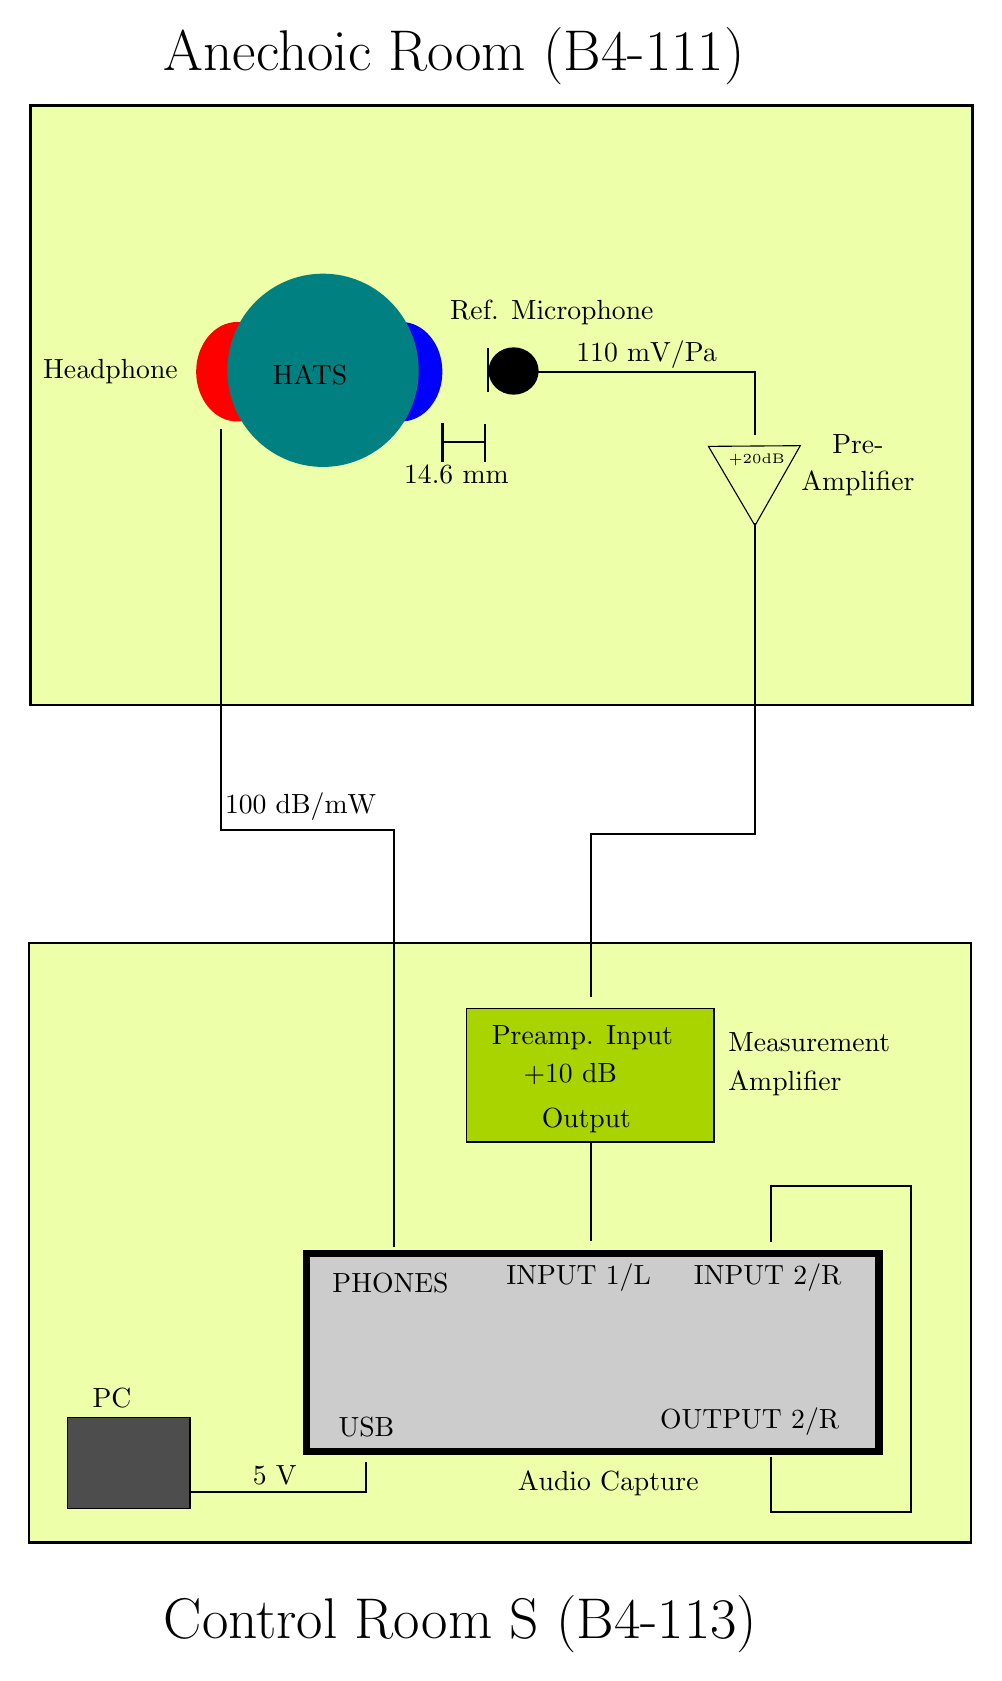
\begin{tikzpicture}[y=0.80pt, x=0.80pt, yscale=-1.000000, xscale=1.000000, inner sep=0pt, outer sep=0pt]
\begin{scope}% layer1
  % rect3342
  \path[draw=black,fill=ceeffaa,line join=miter,line cap=butt,even odd rule,line
    width=0.968pt,rounded corners=0.0000cm] (160.5802,93.3428) rectangle
    (586.0658,364.2491);

  % path3348-0
  \path[fill=c0000ff] (328.0701,213.6738) ellipse (0.5225cm and 0.6318cm);

  % path3348-0-0
  \path[fill=cff0000] (254.0175,213.6738) ellipse (0.5225cm and 0.6318cm);

  % text3399
  \path[fill=black,line join=miter,line cap=butt,line width=0.800pt]
    (220.8386,84.1497) node[above right] (text3399) {\huge{Anechoic Room (B4-111)}};

  % path3415
  \path[draw=black,line join=miter,line cap=butt,even odd rule,line width=0.800pt]
    (367.1652,202.9987) -- (367.1652,222.8035);

  % path3417
  \path[fill=black] (378.8253,213.3426) ellipse (0.3179cm and 0.3007cm);

  % text3425
  \path[fill=black,line join=miter,line cap=butt,line width=0.800pt]
    (407.1953,212.2592) node[above right] (text3425) {110 mV/Pa};

  % path3350-7
  \path[fill=c008080] (292.7422,213.0265) ellipse (1.2151cm and 1.2272cm);

  % path3471
  \path[draw=black,line join=miter,line cap=butt,even odd rule,line width=0.800pt]
    (346.7410,236.9996) -- (346.7410,254.3237);

  % path3471-4
  \path[draw=black,line join=miter,line cap=butt,even odd rule,line width=0.800pt]
    (366.0000,237.2002) -- (366.0000,254.5243);

  % path3488
  \path[draw=black,line join=miter,line cap=butt,even odd rule,line width=0.800pt]
    (347.0127,245.5534) -- (365.8394,245.5534);

  % text3490
  \path[fill=black,line join=miter,line cap=butt,line width=0.800pt]
    (329.3616,264.2414) node[above right] (text3490) {14.6 mm};

  % text3494
  \path[fill=black,line join=miter,line cap=butt,line width=0.800pt]
    (270.0000,219.3622) node[above right] (text3494) {HATS};

  % text3520
  \path[fill=black,line join=miter,line cap=butt,line width=0.800pt]
    (166.3521,219.0369) node[above right] (text3520) {Headphone};

  % text3524
  \path[fill=black,line join=miter,line cap=butt,line width=0.800pt]
    (350.1392,192.5204) node[above right] (text3524) {Ref. Microphone};

  % path3536
  \path[cm={{0.50668,0.86213,-0.86213,0.50668,(553.19003,422.32154)}},draw=black,fill=black,fill
    opacity=0.000] (-153.0817,-14.1755) -- (-194.5745,-14.1755) --
    (-173.8281,-50.1093) -- cycle;

  % path4338
  \path[draw=black,line join=miter,line cap=butt,even odd rule,line width=0.749pt]
    (389.8283,213.8867) -- (487.6847,213.8867) -- (487.6847,242.3189);

  % text4340
  \path[fill=black,line join=miter,line cap=butt,line width=0.800pt]
    (475.9017,256.3146) node[above right] (text4340) {\tiny{+20dB}};

  % text4346
  \path[fill=black,line join=miter,line cap=butt,line width=0.800pt]
    (515.8203,272.6747) node[above right] (text4346) {};

  % text4350
  \path[fill=black,line join=miter,line cap=butt,line width=0.800pt]
  (522.7854,250.5729) node[above right] (text4350) {Pre-};
  
  \path[fill=black,line join=miter,line cap=butt,line width=0.800pt]
    (508.7854,269.5729) node[above right] (text4350) {Amplifier};

  % rect3342-0
  \path[draw=black,fill=ceeffaa,line join=miter,line cap=butt,even odd rule,line
    width=0.968pt,rounded corners=0.0000cm] (159.9447,471.6903) rectangle
    (585.4303,742.5966);

  % text3399-2
  \path[fill=black,line join=miter,line cap=butt,line width=0.800pt]
    (220.8386,792.2573) node[above right] (text3399-2) {\centering{\huge{Control Room S (B4-113)}}};

  % text4387
  \path[fill=black,line join=miter,line cap=butt,line width=0.800pt]
    (285.9375,785.1747) node[above right] (text4387) {};

  % rect4395
  \path[draw=black,fill=ccccccc,line width=2.558pt,rounded corners=0.0000cm]
    (285.0705,611.9925) rectangle (543.8727,701.3781);

  % rect4397
  \path[draw=black,fill=c4d4d4d,line width=0.507pt,rounded corners=0.0000cm]
    (177.3497,685.9109) rectangle (232.6891,727.0794);

  % text4401
  \path[fill=black,line join=miter,line cap=butt,line width=0.800pt]
    (188.6317,681.3109) node[above right] (text4401) {PC};

  % text4405
  \path[fill=black,line join=miter,line cap=butt,line width=0.800pt]
    (380.7714,721.5567) node[above right] (text4405) {Audio Capture};

  % text4409
  \path[fill=black,line join=miter,line cap=butt,line width=0.800pt]
    (299.7695,694.7996) node[above right] (text4409) {USB};

  % path4417
  \path[draw=black,line join=miter,line cap=butt,even odd rule,line width=0.428pt]
    (232.8075,719.6862) -- (312.1120,719.6862) -- (312.1120,705.9801);

  % text5031
  \path[fill=black,line join=miter,line cap=butt,line width=0.800pt]
    (261.0862,716.0892) node[above right] (text5031) {5 V};

  % text5035
  \path[fill=black,line join=miter,line cap=butt,line width=0.800pt]
    (297.0000,629.3622) node[above right] (text5035) {PHONES};

  % path5039
  \path[draw=black,line join=miter,line cap=butt,even odd rule,line width=0.689pt]
    (324.9365,609.1651) -- (324.9365,420.7478) -- (246.6966,420.7478) --
    (246.6966,239.4242);

  % text5315
  \path[fill=black,line join=miter,line cap=butt,line width=0.800pt]
    (248.4749,416.5442) node[above right] (text5315) {100 dB/mW};

  % text5319
  \path[fill=black,line join=miter,line cap=butt,line width=0.800pt]
    (375.5305,629.0000) node[above right] (text5319) {INPUT 1/L};

  % path6749
  \path[draw=black,line join=miter,line cap=butt,even odd rule,line width=0.677pt]
    (487.8216,282.0222) -- (487.8216,422.5549) -- (413.5950,422.5549) --
    (413.5950,496.2119);

  % text5319-3
  \path[fill=black,line join=miter,line cap=butt,line width=0.800pt]
    (460.2651,629.0000) node[above right] (text5319-3) {INPUT 2/R};

  % text7847
  \path[fill=black,line join=miter,line cap=butt,line width=0.800pt]
    (445.0128,693.9413) node[above right] (text7847) {OUTPUT 2/R};

  % path7851
  \path[draw=black,line join=miter,line cap=butt,even odd rule,line width=0.684pt]
    (495.1485,703.8376) -- (495.1485,728.7909) -- (558.3474,728.7909) --
    (558.3474,581.4711) -- (495.1485,581.4711) -- (495.1485,606.8978);

  % rect10551
  \path[draw=black,fill=caad400,rounded corners=0.0000cm] (357.6139,501.4652)
    rectangle (469.3367,561.5693);

  % path10883
  \path[draw=black,line join=miter,line cap=butt,even odd rule,line width=0.716pt]
    (414.0000,561.8622) -- (414.0000,606.1778);

  % text11321
  \path[fill=black,line join=miter,line cap=butt,line width=0.800pt]
    (475.8738,520.7976) node[above right] (text11321) {Measurement};
  
  \path[fill=black,line join=miter,line cap=butt,line width=0.800pt]
    (475.8738,540.7976) node[above right] (text11321) {Amplifier};

  % text11325
  \path[fill=black,line join=miter,line cap=butt,line width=0.800pt]
    (383.3500,535.6852) node[above right] (text11325) {+10 dB};

  % text11329
  \path[fill=black,line join=miter,line cap=butt,line width=0.800pt]
    (368.9959,520.0778) node[above right] (text11329) {Preamp. Input};

  % text11333
  \path[fill=black,line join=miter,line cap=butt,line width=0.800pt]
    (391.5484,557.4692) node[above right] (text11333) {Output};

\end{scope}
\end{tikzpicture}
}

	\caption{test}
	\label{test}
\end{figure}

\subsection{Settings/Description}
\label{SettingsHeadPhones}

Calibration of the microphone and associated preamplifier is done on the measurement amplifier, but any other method can be used. The following setting is present:
\subsubsection{Control and calibration}
\begin{itemize}
	\item 93.6 dB @ 1000 Hz is used as calibration signal
	\item Microphone sensitivity is controlled to 110 $m$V/Pa
	\item Measurement amplifier is set to -10 dB default
	\item Calibration signal yields an amplitude of 0.87 relative to 0 dBFS
\end{itemize}
\subsubsection{Equipment settings}
\begin{itemize}
	\item This experiment is performed with a sampling rate of, $F_{s}$ = 24,000 Hz
	\item Outside microphone is placed 12.6 mm from headphone cup
	\item For item 4 (sound capture card):
	\begin{itemize}
		\item "SENS(INPUT 1/L)" is set to +0 dB"
		\item "SENS(INPUT 2/R)" is set to +0 dB"
		\item "PHONES" is set to maximum volume
	\end{itemize}		
	\item For item 6 (measuring amplifier):
		\begin{itemize}
			\item "Input Section Gain" is set to +20 dB in proportion to calibration
			\item 22.4 $k$Hz low-pass filter is enabled
			\item 22.4 $k$Hz high-pass filter is enabled 
		\end{itemize}
	\item Item 5 (computer) is set to 0 dBFS
\end{itemize}



\subsubsection{Picture}
\begin{figure}[H]
	\centering
	\includegraphics[width=0.8\textwidth]{CancellationPath_and_Headphones/CloseUpMicNew.jpg}
	\caption{Full setup of experiment.}
	\label{CloseupCancellationPath}
\end{figure}

%\begin{figure}[H]
%	\centering
%	\includegraphics[width=0.8\textwidth]{CancellationPath_and_Headphones/CloseUpMic.jpg}
%	\caption{Close up of experiment.}
%	\label{CloseUpCancellationPath}
%\end{figure}

\subsection{Procedure}
\subsubsection{Set-up}
\begin{enumerate}
	\item Set instruments to comply with the list in \ref{SettingsHeadPhones}
	\item Control, and if necessary, calibrate item 2 using item 7
	\item Place item 3 onto item 1 ("Henry"'s head and ears)
	\item Insert item 2's onto item 8 and connect to input of item 6
	\item Connect item 6 to item 4 and connect item 4 to item 5 via USB
	\item Insert item 3's connector into output of item 4
\end{enumerate}

\subsubsection{Performing the experiment}
\begin{enumerate}
	\item Open Simulink\textsuperscript{\textregistered} and run file "SimulinkSystemHeadPhone.xls"
	\item Through Simulink\textsuperscript{\textregistered} play "LogChirp.wav" from item 5 via item 4
	\item Record and save, and name "Mic[i].wav" and Ref[i].wav" from item 4 onto item 5 \footnote{[i] indicates the iteration of the experiment}
	\begin{itemize}
		\item[] Perform this experiment for a total of 5 times
	\end{itemize}
\end{enumerate}


\subsubsection{Data Extraction}
\begin{enumerate}
	\item Place generated .wav-files in same folder as MATLAB\textsuperscript{\textregistered}-script "HeadPhoneScript.m".
	\item Open MATLAB\textsuperscript{\textregistered} and run script "CancellationPathScript.m"
\end{enumerate}
This should yield the resulting frequency response, impulse response and finally the transfer function, along other information about the headphones in this set-up.


%In MATLAB\textsuperscript{\textregistered} run script: "Headphone\_TF.m" and load file "Headphone\_Path\_1.wav". This should yield the resulting transfer-function and other information about the headphones used in this set-up.\\
%\indent The script takes the sound played by the headphones (Item 2) , applies FFT, and takes the inverse of the result. This result is then convolved with the FFT of the sound picked up by the microphone (Item 5). This yields an impulse response, which is used to determine the transfer-function.
%\todo[inline]{Tjek lige det her}

\subsection{Analysis}
From the performing of the experiment, 10 files has been generated:
\begin{itemize}
	\item HPMic1.wav - HPMic5.wav
	\item HPRef1.wav - HPRef5.wav
\end{itemize}

These files are the results of performing the six second simulation which gives a number of 288,768 samples, for each generated .wav-file.
An example showing outputted Mic1 and Ref1 are shown in  \autoref{HeadPhoneAmplitudePlot}.

%\begin{figure}[H]
%	\centering
%	\tikzsetnextfilename{HeadPhoneAmplitudePlot}
%	% This file was created by matlab2tikz.
%
%The latest updates can be retrieved from
%  http://www.mathworks.com/matlabcentral/fileexchange/22022-matlab2tikz-matlab2tikz
%where you can also make suggestions and rate matlab2tikz.
%
\definecolor{mycolor1}{rgb}{0.00000,0.44700,0.74100}%
\definecolor{mycolor2}{rgb}{0.85000,0.32500,0.09800}%
%
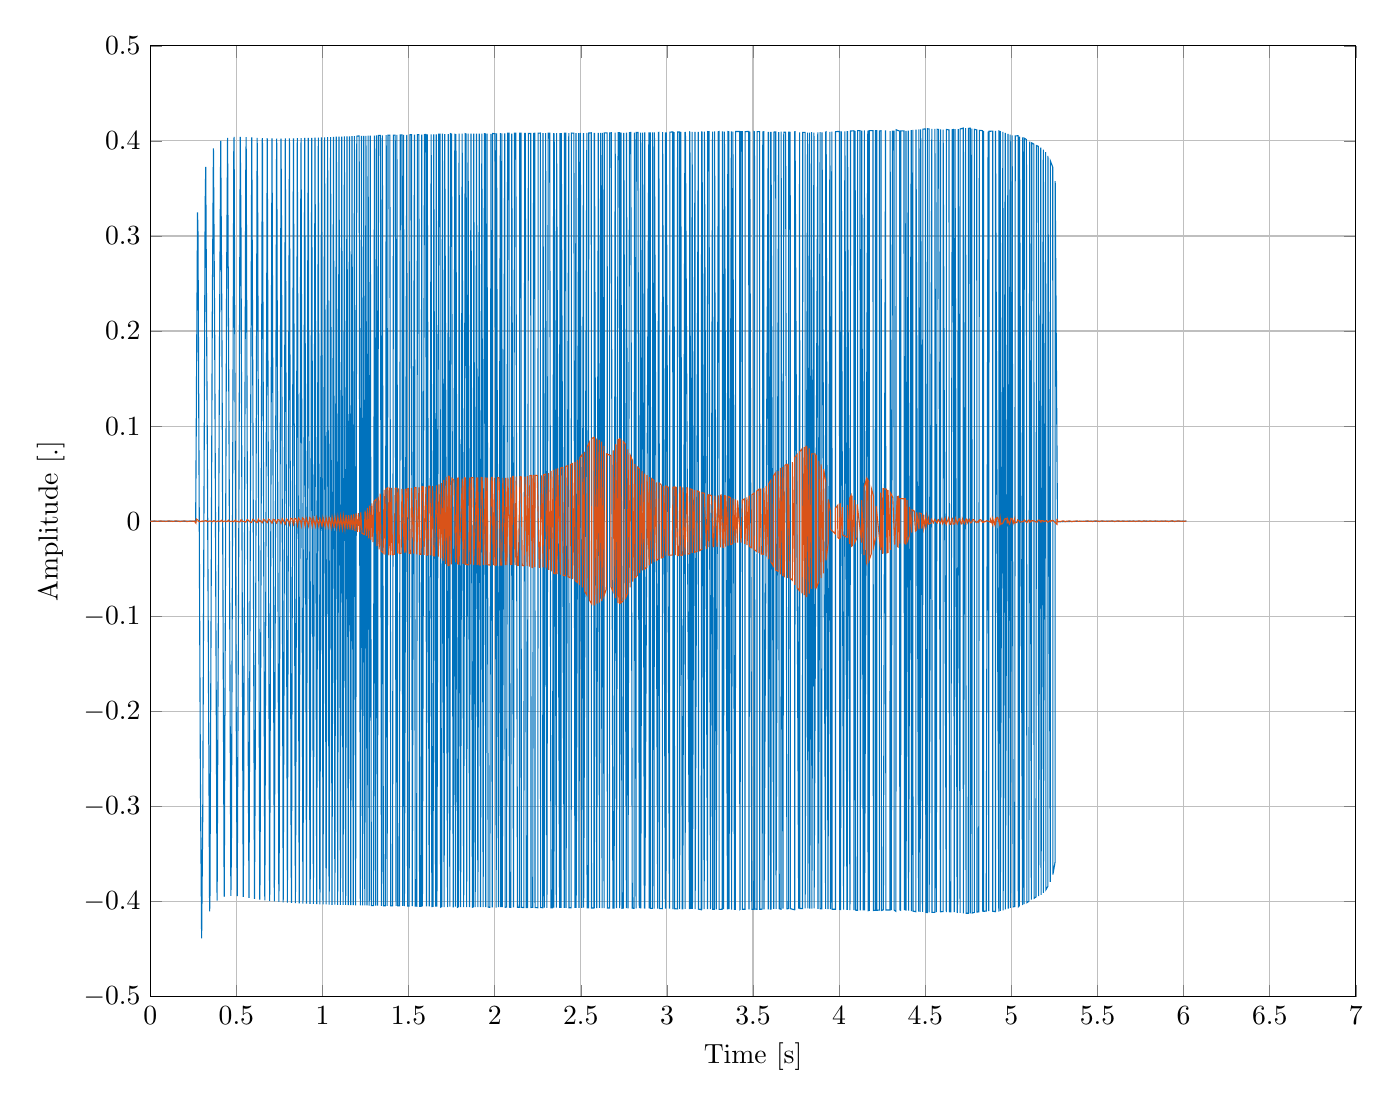
\begin{tikzpicture}

\begin{axis}[%
width=6.028in,
height=4.754in,
at={(1.011in,0.642in)},
scale only axis,
xmin=0,
xmax=7,
xlabel={Time [s]},
xmajorgrids,
ymin=-0.5,
ymax=0.5,
ylabel={Amplitude [.]},
ymajorgrids,
axis background/.style={fill=white}
]
\addplot [color=mycolor1,solid,forget plot]
  table[row sep=crcr]{%
2.08333333333333e-05	0\\
0.00160416666666667	3.0517578125e-05\\
0.00666666666666667	-9.1552734375e-05\\
0.0148125	-6.103515625e-05\\
0.0263541666666667	6.103515625e-05\\
0.028	3.0517578125e-05\\
0.0290416666666667	-6.103515625e-05\\
0.0421041666666667	-6.103515625e-05\\
0.0474791666666667	6.103515625e-05\\
0.0554791666666667	-6.103515625e-05\\
0.0555833333333333	3.0517578125e-05\\
0.0794791666666667	6.103515625e-05\\
0.0805833333333333	-9.1552734375e-05\\
0.0833125	3.0517578125e-05\\
0.084	-9.1552734375e-05\\
0.09725	-6.103515625e-05\\
0.0977291666666667	6.103515625e-05\\
0.110979166666667	-6.103515625e-05\\
0.111479166666667	3.0517578125e-05\\
0.124833333333333	-6.103515625e-05\\
0.125375	6.103515625e-05\\
0.138833333333333	3.0517578125e-05\\
0.139854166666667	-9.1552734375e-05\\
0.1526875	3.0517578125e-05\\
0.15275	-6.103515625e-05\\
0.166541666666667	-6.103515625e-05\\
0.1766875	6.103515625e-05\\
0.180229166666667	3.0517578125e-05\\
0.180625	-6.103515625e-05\\
0.1950625	6.103515625e-05\\
0.196	-9.1552734375e-05\\
0.208	-6.103515625e-05\\
0.219125	6.103515625e-05\\
0.222895833333333	6.103515625e-05\\
0.223354166666667	-9.1552734375e-05\\
0.236604166666667	6.103515625e-05\\
0.237395833333333	-9.1552734375e-05\\
0.249625	-6.103515625e-05\\
0.256083333333333	6.103515625e-05\\
0.263916666666667	-6.103515625e-05\\
0.274604166666667	0.3248291015625\\
0.277270833333333	0.302764892578125\\
0.291125	-0.2672119140625\\
0.291125	-0.2672119140625\\
0.298375	-0.43878173828125\\
0.304979166666667	-0.308990478515625\\
0.318854166666667	0.331085205078125\\
0.322208333333333	0.372711181640625\\
0.332708333333333	0.03741455078125\\
0.332708333333333	0.03741455078125\\
0.344791666666667	-0.410430908203125\\
0.346583333333333	-0.3988037109375\\
0.3604375	0.2232666015625\\
0.3669375	0.391998291015625\\
0.374291666666667	0.19525146484375\\
0.374291666666667	0.19525146484375\\
0.388145833333333	-0.39886474609375\\
0.3883125	-0.399078369140625\\
0.402020833333333	0.1805419921875\\
0.402020833333333	0.1805419921875\\
0.409166666666667	0.40008544921875\\
0.415875	0.212432861328125\\
0.429291666666667	-0.394927978515625\\
0.42975	-0.3941650390625\\
0.443604166666667	0.257049560546875\\
0.449020833333333	0.403289794921875\\
0.457458333333333	0.08868408203125\\
0.457458333333333	0.08868408203125\\
0.46825	-0.393951416015625\\
0.471333333333333	-0.34320068359375\\
0.4851875	0.388763427734375\\
0.486791666666667	0.404266357421875\\
0.4990625	-0.198883056640625\\
0.504979166666667	-0.394317626953125\\
0.512916666666667	-0.072113037109375\\
0.512916666666667	-0.072113037109375\\
0.522625	0.404266357421875\\
0.526770833333333	0.3067626953125\\
0.539958333333333	-0.3951416015625\\
0.540645833333333	-0.392425537109375\\
0.5545	0.36322021484375\\
0.5569375	0.40399169921875\\
0.568354166666667	-0.221435546875\\
0.5734375	-0.3961181640625\\
0.582229166666667	0.05206298828125\\
0.582229166666667	0.05206298828125\\
0.589520833333333	0.403594970703125\\
0.596083333333333	0.11871337890625\\
0.605354166666667	-0.397125244140625\\
0.6099375	-0.244110107421875\\
0.620791666666667	0.40325927734375\\
0.6238125	0.332000732421875\\
0.635916666666667	-0.397979736328125\\
0.637666666666667	-0.373565673828125\\
0.650708333333333	0.40289306640625\\
0.651541666666667	0.39739990234375\\
0.665270833333333	-0.398681640625\\
0.665395833333333	-0.39849853515625\\
0.67925	0.402099609375\\
0.679458333333333	0.402740478515625\\
0.693125	-0.39825439453125\\
0.6935	-0.399383544921875\\
0.706979166666667	0.402252197265625\\
0.707166666666667	0.402618408203125\\
0.720604166666667	-0.399932861328125\\
0.720833333333333	-0.399322509765625\\
0.733770833333333	0.402496337890625\\
0.734708333333333	0.3934326171875\\
0.746770833333333	-0.400421142578125\\
0.7485625	-0.36358642578125\\
0.7594375	0.402496337890625\\
0.762416666666667	0.301910400390625\\
0.7719375	-0.400848388671875\\
0.776291666666667	-0.187744140625\\
0.78425	0.402587890625\\
0.796354166666667	-0.401123046875\\
0.804	0.169281005859375\\
0.808229166666667	0.402587890625\\
0.817875	-0.3397216796875\\
0.819958333333333	-0.4014892578125\\
0.831479166666667	0.4027099609375\\
0.831729166666667	0.401763916015625\\
0.842833333333333	-0.401702880859375\\
0.845604166666667	-0.28765869140625\\
0.853958333333333	0.40283203125\\
0.8649375	-0.40191650390625\\
0.8733125	0.302520751953125\\
0.875791666666667	0.40289306640625\\
0.886416666666667	-0.402099609375\\
0.8871875	-0.392791748046875\\
0.896958333333333	0.403045654296875\\
0.907291666666667	-0.40228271484375\\
0.914895833333333	0.27691650390625\\
0.917520833333333	0.403106689453125\\
0.927583333333333	-0.402435302734375\\
0.928770833333333	-0.376220703125\\
0.937520833333333	0.40325927734375\\
0.9473125	-0.402557373046875\\
0.956479166666667	0.39788818359375\\
0.956958333333333	0.403411865234375\\
0.966520833333333	-0.4027099609375\\
0.9759375	0.403533935546875\\
0.984208333333333	-0.3792724609375\\
0.985229166666667	-0.40289306640625\\
0.994416666666667	0.403656005859375\\
1.00345833333333	-0.4029541015625\\
1.0119375	0.3980712890625\\
1.01241666666667	0.403778076171875\\
1.02125	-0.403045654296875\\
1.03	0.40386962890625\\
1.0385625	-0.40313720703125\\
1.03966666666667	-0.373687744140625\\
1.04716666666667	0.404052734375\\
1.05554166666667	-0.403411865234375\\
1.063875	0.40423583984375\\
1.072125	-0.403289794921875\\
1.08027083333333	0.40435791015625\\
1.08125	0.37530517578125\\
1.08829166666667	-0.40350341796875\\
1.09629166666667	0.404449462890625\\
1.104125	-0.403533935546875\\
1.11195833333333	0.404541015625\\
1.11966666666667	-0.403656005859375\\
1.12727083333333	0.4046630859375\\
1.13479166666667	-0.403656005859375\\
1.1423125	0.40478515625\\
1.1496875	-0.40374755859375\\
1.15702083333333	0.40478515625\\
1.16427083333333	-0.403839111328125\\
1.16441666666667	-0.40277099609375\\
1.17141666666667	0.4049072265625\\
1.1785	-0.40380859375\\
1.1855625	0.40496826171875\\
1.19252083333333	-0.4039306640625\\
1.1994375	0.405059814453125\\
1.21304166666667	0.405120849609375\\
1.21975	-0.404022216796875\\
1.22639583333333	0.405242919921875\\
1.23297916666667	-0.404083251953125\\
1.2395	0.40533447265625\\
1.24595833333333	-0.404083251953125\\
1.252375	0.40533447265625\\
1.25872916666667	-0.4041748046875\\
1.26502083333333	0.405426025390625\\
1.27129166666667	-0.404205322265625\\
1.27747916666667	0.405517578125\\
1.28360416666667	-0.40423583984375\\
1.29572916666667	-0.404296875\\
1.30170833333333	0.405609130859375\\
1.307625	-0.404296875\\
1.31354166666667	0.40570068359375\\
1.31939583333333	-0.404327392578125\\
1.3251875	0.405731201171875\\
1.336625	0.40582275390625\\
1.34229166666667	-0.404449462890625\\
1.34789583333333	0.405853271484375\\
1.35347916666667	-0.4044189453125\\
1.36447916666667	-0.404449462890625\\
1.36995833333333	0.405975341796875\\
1.37533333333333	-0.40447998046875\\
1.38070833333333	0.406005859375\\
1.3913125	0.406005859375\\
1.39658333333333	-0.404571533203125\\
1.40695833333333	-0.404541015625\\
1.41210416666667	0.406097412109375\\
1.42225	0.406097412109375\\
1.42729166666667	-0.40460205078125\\
1.43229166666667	0.40618896484375\\
1.43725	-0.404632568359375\\
1.4470625	-0.404632568359375\\
1.45191666666667	0.40625\\
1.46154166666667	0.40625\\
1.4663125	-0.404693603515625\\
1.4710625	0.406341552734375\\
1.47577083333333	-0.40472412109375\\
1.4896875	0.4063720703125\\
1.49427083333333	-0.404754638671875\\
1.50335416666667	-0.404754638671875\\
1.50783333333333	0.406402587890625\\
1.51677083333333	0.40643310546875\\
1.52116666666667	-0.40484619140625\\
1.53425	0.406494140625\\
1.5385625	-0.40484619140625\\
1.547125	-0.4049072265625\\
1.55133333333333	0.40655517578125\\
1.55972916666667	0.40655517578125\\
1.56389583333333	-0.40496826171875\\
1.57214583333333	-0.404937744140625\\
1.57625	0.4066162109375\\
1.5803125	-0.404998779296875\\
1.59239583333333	0.406646728515625\\
1.6003125	0.406707763671875\\
1.60425	-0.405120849609375\\
1.60816666666667	0.40673828125\\
1.61979166666667	-0.405120849609375\\
1.63120833333333	0.40679931640625\\
1.635	-0.40521240234375\\
1.64245833333333	-0.4051513671875\\
1.64620833333333	0.4068603515625\\
1.65720833333333	-0.4052734375\\
1.66085416666667	0.4068603515625\\
1.66447916666667	-0.405303955078125\\
1.67522916666667	0.406951904296875\\
1.6823125	0.406951904296875\\
1.68583333333333	-0.405914306640625\\
1.6928125	-0.405303955078125\\
1.69627083333333	0.407562255859375\\
1.7065625	-0.405975341796875\\
1.70995833333333	0.407012939453125\\
1.72670833333333	-0.4058837890625\\
1.73004166666667	0.40704345703125\\
1.73985416666667	-0.405426025390625\\
1.74310416666667	0.407623291015625\\
1.7495625	0.4071044921875\\
1.759125	-0.406036376953125\\
1.76858333333333	0.407623291015625\\
1.7716875	-0.40545654296875\\
1.7748125	0.407135009765625\\
1.78404166666667	-0.406036376953125\\
1.79014583333333	-0.405426025390625\\
1.79316666666667	0.407623291015625\\
1.8021875	-0.406005859375\\
1.81108333333333	0.407623291015625\\
1.819875	-0.406005859375\\
1.8285625	0.4075927734375\\
1.83429166666667	0.407196044921875\\
1.83714583333333	-0.405975341796875\\
1.845625	0.4075927734375\\
1.85402083333333	-0.40594482421875\\
1.8623125	0.40765380859375\\
1.87052083333333	-0.405975341796875\\
1.87591666666667	-0.4056396484375\\
1.87860416666667	0.407684326171875\\
1.886625	-0.405975341796875\\
1.8945625	0.4075927734375\\
1.90239583333333	-0.40594482421875\\
1.91016666666667	0.40765380859375\\
1.91783333333333	-0.405975341796875\\
1.9254375	0.407623291015625\\
1.9329375	-0.405914306640625\\
1.940375	0.407470703125\\
1.94529166666667	0.407440185546875\\
1.94775	-0.40582275390625\\
1.95502083333333	0.407562255859375\\
1.96225	-0.40594482421875\\
1.97175	-0.406005859375\\
1.9788125	0.407501220703125\\
1.98579166666667	-0.40618896484375\\
1.98810416666667	0.407745361328125\\
2.00183333333333	0.407501220703125\\
2.00860416666667	-0.406341552734375\\
2.01083333333333	0.407806396484375\\
2.0219375	-0.405914306640625\\
2.032875	0.408050537109375\\
2.03504166666667	-0.405975341796875\\
2.0415	0.407958984375\\
2.04364583333333	-0.40594482421875\\
2.05847916666667	0.407989501953125\\
2.0605625	-0.405975341796875\\
2.068875	-0.40594482421875\\
2.07504166666667	0.408050537109375\\
2.0831875	0.408050537109375\\
2.08520833333333	-0.405975341796875\\
2.09325	-0.406158447265625\\
2.09920833333333	0.40765380859375\\
2.10904166666667	-0.406036376953125\\
2.114875	0.408050537109375\\
2.12260416666667	0.40802001953125\\
2.132125	-0.406036376953125\\
2.14339583333333	-0.406005859375\\
2.14525	0.408050537109375\\
2.15264583333333	0.4080810546875\\
2.15447916666667	-0.4061279296875\\
2.16902083333333	-0.4063720703125\\
2.17439583333333	0.407745361328125\\
2.17795833333333	0.40777587890625\\
2.18327083333333	-0.406341552734375\\
2.19029166666667	-0.40625\\
2.1955	0.407806396484375\\
2.20925	0.407806396484375\\
2.2109375	-0.40625\\
2.2210625	-0.4061279296875\\
2.2260625	0.407928466796875\\
2.2326875	0.407989501953125\\
2.23433333333333	-0.4063720703125\\
2.25058333333333	-0.406524658203125\\
2.2521875	0.408050537109375\\
2.26489583333333	0.408233642578125\\
2.26647916666667	-0.406341552734375\\
2.2789375	-0.406524658203125\\
2.28047916666667	0.408111572265625\\
2.28814583333333	-0.406494140625\\
2.29575	0.408203125\\
2.30325	-0.40655517578125\\
2.3106875	0.408203125\\
2.3195	0.408203125\\
2.32677083333333	-0.40655517578125\\
2.33539583333333	-0.406524658203125\\
2.3425	0.40814208984375\\
2.34391666666667	-0.406463623046875\\
2.34533333333333	0.407958984375\\
2.35791666666667	-0.406494140625\\
2.35929166666667	0.408111572265625\\
2.37704166666667	-0.40655517578125\\
2.37839583333333	0.40814208984375\\
2.38510416666667	-0.40655517578125\\
2.3864375	0.408172607421875\\
2.40354166666667	-0.4066162109375\\
2.40485416666667	0.408172607421875\\
2.41260416666667	0.408203125\\
2.413875	-0.40655517578125\\
2.43035416666667	0.40826416015625\\
2.43160416666667	-0.406524658203125\\
2.44402083333333	-0.406646728515625\\
2.44525	0.408233642578125\\
2.45983333333333	0.408203125\\
2.46583333333333	-0.40667724609375\\
2.47177083333333	0.408203125\\
2.47295833333333	-0.406768798828125\\
2.48816666666667	0.408172607421875\\
2.4893125	-0.4066162109375\\
2.49735416666667	0.408355712890625\\
2.5053125	-0.406707763671875\\
2.51541666666667	0.40826416015625\\
2.51652083333333	-0.406494140625\\
2.53520833333333	0.4083251953125\\
2.53629166666667	-0.406646728515625\\
2.54489583333333	-0.40667724609375\\
2.54595833333333	0.40826416015625\\
2.56077083333333	0.408477783203125\\
2.5618125	-0.4068603515625\\
2.5763125	-0.406768798828125\\
2.57733333333333	0.408447265625\\
2.57835416666667	-0.40679931640625\\
2.579375	0.40838623046875\\
2.59252083333333	-0.406829833984375\\
2.60147916666667	0.408538818359375\\
2.608375	-0.406768798828125\\
2.61520833333333	0.408447265625\\
2.62389583333333	-0.406829833984375\\
2.62485416666667	0.408538818359375\\
2.6353125	-0.406829833984375\\
2.63625	0.408447265625\\
2.65304166666667	0.408477783203125\\
2.65395833333333	-0.406829833984375\\
2.66672916666667	-0.4068603515625\\
2.667625	0.40838623046875\\
2.67660416666667	0.40850830078125\\
2.68635416666667	-0.406951904296875\\
2.69335416666667	-0.4068603515625\\
2.6994375	0.40863037109375\\
2.70716666666667	-0.406890869140625\\
2.71652083333333	0.408599853515625\\
2.72491666666667	0.40863037109375\\
2.72575	-0.406951904296875\\
2.73320833333333	0.408599853515625\\
2.73895833333333	-0.40704345703125\\
2.74710416666667	-0.40692138671875\\
2.74952083333333	0.408538818359375\\
2.7646875	-0.40692138671875\\
2.76547916666667	0.4085693359375\\
2.77410416666667	-0.407135009765625\\
2.782625	0.408721923828125\\
2.79029166666667	0.4088134765625\\
2.798625	-0.406982421875\\
2.80910416666667	-0.4071044921875\\
2.81133333333333	0.40875244140625\\
2.82089583333333	-0.4071044921875\\
2.821625	0.408782958984375\\
2.83177083333333	0.4088134765625\\
2.83964583333333	-0.40704345703125\\
2.8474375	0.408782958984375\\
2.84814583333333	-0.40716552734375\\
2.858625	0.4088134765625\\
2.86895833333333	-0.407318115234375\\
2.871	0.409027099609375\\
2.8716875	-0.40753173828125\\
2.89514583333333	0.408935546875\\
2.897125	-0.4072265625\\
2.90302083333333	0.40899658203125\\
2.90366666666667	-0.407257080078125\\
2.9153125	-0.4072265625\\
2.91722916666667	0.408843994140625\\
2.9255	-0.407379150390625\\
2.92739583333333	0.4090576171875\\
2.9466875	-0.407379150390625\\
2.95097916666667	0.40887451171875\\
2.95341666666667	0.408966064453125\\
2.95766666666667	-0.407379150390625\\
2.97322916666667	-0.40753173828125\\
2.975	0.4093017578125\\
2.99077083333333	-0.40740966796875\\
2.99135416666667	0.408966064453125\\
2.99422916666667	-0.40740966796875\\
2.99595833333333	0.40899658203125\\
3.01464583333333	-0.40740966796875\\
3.0174375	0.40911865234375\\
3.03395833333333	0.409515380859375\\
3.0345	-0.407867431640625\\
3.04154166666667	0.40911865234375\\
3.04422916666667	-0.4075927734375\\
3.06120833333333	-0.40777587890625\\
3.06172916666667	0.409332275390625\\
3.07316666666667	0.409332275390625\\
3.0736875	-0.407623291015625\\
3.08035416666667	0.409423828125\\
3.08897916666667	-0.407684326171875\\
3.092	-0.4075927734375\\
3.10445833333333	0.409332275390625\\
3.1059375	-0.40765380859375\\
3.10741666666667	0.409393310546875\\
3.131125	-0.40789794921875\\
3.13160416666667	0.409393310546875\\
3.1335	0.40924072265625\\
3.13964583333333	-0.40777587890625\\
3.14666666666667	0.409423828125\\
3.1480625	-0.407806396484375\\
3.16325	0.4095458984375\\
3.16370833333333	-0.407958984375\\
3.182125	0.409423828125\\
3.18345833333333	-0.40802001953125\\
3.19922916666667	-0.40863037109375\\
3.20139583333333	0.409942626953125\\
3.2026875	-0.408416748046875\\
3.20397916666667	0.40985107421875\\
3.21635416666667	-0.40802001953125\\
3.217625	0.40960693359375\\
3.2355625	-0.408050537109375\\
3.23597916666667	0.4097900390625\\
3.24416666666667	0.40966796875\\
3.25266666666667	-0.40802001953125\\
3.26504166666667	0.409637451171875\\
3.26622916666667	-0.40814208984375\\
3.27564583333333	-0.408233642578125\\
3.2768125	0.409942626953125\\
3.28647916666667	-0.408294677734375\\
3.29829166666667	0.409576416015625\\
3.3028125	0.40985107421875\\
3.3031875	-0.40826416015625\\
3.32025	-0.40814208984375\\
3.3228125	0.410064697265625\\
3.32827083333333	-0.4080810546875\\
3.3336875	0.40960693359375\\
3.3518125	-0.408233642578125\\
3.3535625	0.40985107421875\\
3.35914583333333	0.409637451171875\\
3.3601875	-0.408111572265625\\
3.37427083333333	0.41009521484375\\
3.37529166666667	-0.408599853515625\\
3.3830625	0.409759521484375\\
3.39208333333333	-0.40826416015625\\
3.397375	-0.408172607421875\\
3.39902083333333	0.40985107421875\\
3.4223125	0.409881591796875\\
3.42327083333333	-0.40850830078125\\
3.42454166666667	-0.4083251953125\\
3.42991666666667	0.4097900390625\\
3.4380625	0.4097900390625\\
3.438375	-0.408172607421875\\
3.45316666666667	-0.408172607421875\\
3.45408333333333	0.40972900390625\\
3.47510416666667	0.409942626953125\\
3.47658333333333	-0.408355712890625\\
3.481	0.40960693359375\\
3.4929375	-0.408111572265625\\
3.50439583333333	-0.408294677734375\\
3.50525	0.409820556640625\\
3.50808333333333	0.409576416015625\\
3.510625	-0.408050537109375\\
3.52291666666667	-0.4080810546875\\
3.52375	0.409698486328125\\
3.53854166666667	0.409759521484375\\
3.5388125	-0.40814208984375\\
3.55277083333333	-0.408050537109375\\
3.55675	0.409423828125\\
3.56254166666667	0.40960693359375\\
3.56385416666667	-0.408203125\\
3.5883125	0.4095458984375\\
3.5885625	-0.40814208984375\\
3.60135416666667	0.409576416015625\\
3.60160416666667	-0.407989501953125\\
3.60408333333333	-0.407928466796875\\
3.60433333333333	0.40936279296875\\
3.62025	-0.407745361328125\\
3.62145833333333	0.409271240234375\\
3.63202083333333	0.409393310546875\\
3.6336875	-0.40777587890625\\
3.64897916666667	0.4093017578125\\
3.652	-0.407562255859375\\
3.66258333333333	-0.408111572265625\\
3.6628125	0.409637451171875\\
3.67391666666667	-0.407562255859375\\
3.678625	0.4090576171875\\
3.68927083333333	0.409027099609375\\
3.6969375	-0.407562255859375\\
3.70645833333333	-0.40753173828125\\
3.70710416666667	0.40911865234375\\
3.71564583333333	0.409027099609375\\
3.71670833333333	-0.407501220703125\\
3.74170833333333	-0.408660888671875\\
3.74191666666667	0.40997314453125\\
3.7429375	-0.408905029296875\\
3.74395833333333	0.41021728515625\\
3.76508333333333	-0.40740966796875\\
3.77041666666667	0.408966064453125\\
3.77041666666667	0.408966064453125\\
3.7721875	-0.4073486328125\\
3.78695833333333	-0.407440185546875\\
3.7886875	0.408966064453125\\
3.802375	0.408843994140625\\
3.8025625	-0.407318115234375\\
3.81691666666667	0.4088134765625\\
3.81820833333333	-0.40728759765625\\
3.82827083333333	0.4088134765625\\
3.82954166666667	-0.4073486328125\\
3.84016666666667	0.409149169921875\\
3.84141666666667	-0.407562255859375\\
3.853625	0.4088134765625\\
3.8545	-0.407196044921875\\
3.87608333333333	0.409027099609375\\
3.87727083333333	-0.407745361328125\\
3.8895625	0.409088134765625\\
3.88972916666667	-0.407562255859375\\
3.8986875	-0.40771484375\\
3.9005	0.4090576171875\\
3.92172916666667	-0.407684326171875\\
3.92220833333333	0.4093017578125\\
3.9244375	0.409515380859375\\
3.93533333333333	-0.40789794921875\\
3.946375	0.409454345703125\\
3.94991666666667	-0.4080810546875\\
3.95770833333333	0.409637451171875\\
3.95877083333333	-0.408111572265625\\
3.9779375	-0.408172607421875\\
3.97808333333333	0.409576416015625\\
3.97970833333333	-0.408416748046875\\
3.97985416666667	0.4097900390625\\
4.00191666666667	0.40985107421875\\
4.00291666666667	-0.4083251953125\\
4.00860416666667	-0.40838623046875\\
4.01185416666667	0.409942626953125\\
4.02595833333333	-0.4085693359375\\
4.03325	0.41009521484375\\
4.0450625	-0.408660888671875\\
4.0468125	0.4102783203125\\
4.04775	-0.408721923828125\\
4.04895833333333	0.410247802734375\\
4.062625	-0.408935546875\\
4.06616666666667	0.410369873046875\\
4.08527083333333	0.410614013671875\\
4.08641666666667	-0.409088134765625\\
4.092875	0.41064453125\\
4.09627083333333	-0.409088134765625\\
4.10722916666667	-0.409332275390625\\
4.10735416666667	0.410797119140625\\
4.1210625	0.41082763671875\\
4.12239583333333	-0.409332275390625\\
4.13141666666667	0.410919189453125\\
4.13985416666667	-0.409393310546875\\
4.14679166666667	0.4110107421875\\
4.147375	-0.409423828125\\
4.16641666666667	0.410888671875\\
4.16789583333333	-0.409637451171875\\
4.17445833333333	-0.40936279296875\\
4.17502083333333	0.41082763671875\\
4.1963125	0.41070556640625\\
4.19860416666667	-0.409393310546875\\
4.20941666666667	-0.409332275390625\\
4.21016666666667	0.41064453125\\
4.21827083333333	0.410614013671875\\
4.218375	-0.409149169921875\\
4.23389583333333	-0.409088134765625\\
4.234	0.4105224609375\\
4.2436875	0.41064453125\\
4.24583333333333	-0.409393310546875\\
4.25677083333333	-0.40869140625\\
4.26922916666667	0.410369873046875\\
4.269625	0.410369873046875\\
4.27110416666667	-0.40887451171875\\
4.29533333333333	-0.40887451171875\\
4.296	0.41015625\\
4.30272916666667	-0.40899658203125\\
4.30958333333333	0.410125732421875\\
4.3185	0.41021728515625\\
4.31914583333333	-0.40899658203125\\
4.32958333333333	-0.410308837890625\\
4.33058333333333	0.41168212890625\\
4.35116666666667	0.410247802734375\\
4.3523125	-0.408843994140625\\
4.35722916666667	-0.409210205078125\\
4.35766666666667	0.4105224609375\\
4.3763125	0.410430908203125\\
4.37945833333333	-0.409149169921875\\
4.38797916666667	0.410614013671875\\
4.3880625	-0.409454345703125\\
4.4014375	0.410858154296875\\
4.403	-0.409576416015625\\
4.41852083333333	0.4112548828125\\
4.41908333333333	-0.40997314453125\\
4.42810416666667	0.411468505859375\\
4.4285	-0.4100341796875\\
4.44558333333333	-0.4107666015625\\
4.446125	0.411865234375\\
4.46166666666667	-0.41070556640625\\
4.46310416666667	0.412109375\\
4.47025	-0.410980224609375\\
4.4733125	0.412200927734375\\
4.48433333333333	-0.410980224609375\\
4.48616666666667	0.412322998046875\\
4.50052083333333	0.412628173828125\\
4.50345833333333	-0.41143798828125\\
4.5115625	-0.411590576171875\\
4.51191666666667	0.412750244140625\\
4.52202083333333	0.41259765625\\
4.52222916666667	-0.411376953125\\
4.53814583333333	0.412628173828125\\
4.53916666666667	-0.411468505859375\\
4.55558333333333	-0.411407470703125\\
4.55591666666667	0.412506103515625\\
4.5643125	-0.411041259765625\\
4.56883333333333	0.412200927734375\\
4.57779166666667	0.412017822265625\\
4.58810416666667	-0.410919189453125\\
4.5893125	0.4119873046875\\
4.589375	-0.410736083984375\\
4.60370833333333	-0.410614013671875\\
4.60377083333333	0.411773681640625\\
4.62214583333333	-0.411102294921875\\
4.6228125	0.41204833984375\\
4.6378125	0.411529541015625\\
4.640125	-0.41070556640625\\
4.64789583333333	-0.4107666015625\\
4.65691666666667	0.411712646484375\\
4.66279166666667	0.411956787109375\\
4.6685625	-0.411041259765625\\
4.67247916666667	0.41229248046875\\
4.68510416666667	-0.411285400390625\\
4.68677083333333	-0.411376953125\\
4.69158333333333	0.412445068359375\\
4.70214583333333	-0.411956787109375\\
4.70241666666667	0.412506103515625\\
4.72033333333333	0.413421630859375\\
4.72091666666667	-0.412353515625\\
4.73429166666667	0.41339111328125\\
4.7369375	-0.412322998046875\\
4.74966666666667	-0.412353515625\\
4.7509375	0.4132080078125\\
4.761125	0.413330078125\\
4.761375	-0.4124755859375\\
4.77047916666667	0.412811279296875\\
4.7718125	-0.412139892578125\\
4.78520833333333	-0.411468505859375\\
4.78535416666667	0.412139892578125\\
4.79897916666667	0.41156005859375\\
4.80016666666667	-0.4111328125\\
4.8104375	-0.410888671875\\
4.8139375	0.411102294921875\\
4.8326875	0.4107666015625\\
4.83345833333333	-0.410675048828125\\
4.83802083333333	0.41033935546875\\
4.83914583333333	-0.41033935546875\\
4.85383333333333	-0.410003662109375\\
4.86489583333333	0.40985107421875\\
4.86883333333333	-0.410064697265625\\
4.87008333333333	0.41009521484375\\
4.8920625	0.4102783203125\\
4.89210416666667	-0.410247802734375\\
4.90666666666667	-0.41064453125\\
4.90670833333333	0.410491943359375\\
4.9078125	-0.4105224609375\\
4.90785416666667	0.410430908203125\\
4.92702083333333	-0.4105224609375\\
4.92745833333333	0.410400390625\\
4.935375	0.409759521484375\\
4.93572916666667	-0.409820556640625\\
4.950875	0.409423828125\\
4.95214583333333	-0.409271240234375\\
4.9643125	0.408538818359375\\
4.96533333333333	-0.40826416015625\\
4.98039583333333	0.407440185546875\\
4.98154166666667	-0.407562255859375\\
4.99308333333333	0.4066162109375\\
4.99435416666667	-0.40655517578125\\
5.00447916666667	0.405792236328125\\
5.01014583333333	-0.4056396484375\\
5.01945833333333	-0.4052734375\\
5.02229166666667	0.405181884765625\\
5.0390625	0.405426025390625\\
5.0401875	-0.405517578125\\
5.0465625	-0.404266357421875\\
5.04727083333333	0.40435791015625\\
5.06489583333333	-0.403656005859375\\
5.06552083333333	0.40362548828125\\
5.07372916666667	-0.402862548828125\\
5.07454166666667	0.40283203125\\
5.08735416666667	0.401397705078125\\
5.090125	-0.401153564453125\\
5.10141666666667	-0.39971923828125\\
5.1065	0.3992919921875\\
5.11591666666667	-0.39794921875\\
5.11845833333333	0.3978271484375\\
5.13058333333333	0.3966064453125\\
5.131875	-0.3966064453125\\
5.14283333333333	-0.39520263671875\\
5.1458125	0.39508056640625\\
5.15685416666667	0.394256591796875\\
5.15804166666667	-0.39434814453125\\
5.17075	0.392822265625\\
5.1723125	-0.39300537109375\\
5.1855	0.390777587890625\\
5.18558333333333	-0.390777587890625\\
5.19891666666667	0.38812255859375\\
5.20058333333333	-0.38751220703125\\
5.2120625	-0.38397216796875\\
5.21225	0.38427734375\\
5.22589583333333	-0.37945556640625\\
5.22629166666667	0.378875732421875\\
5.240375	0.372283935546875\\
5.24102083333333	-0.371734619140625\\
5.25370833333333	-0.358489990234375\\
5.25429166666667	0.357696533203125\\
5.26747916666667	-0.000640869140625\\
5.27741666666667	-0.00048828125\\
5.28145833333333	-0.000579833984375\\
5.29427083333333	-0.00042724609375\\
5.29552083333333	-0.000518798828125\\
5.307625	-0.0003662109375\\
5.30947916666667	-0.00048828125\\
5.31802083333333	-0.00030517578125\\
5.32308333333333	-0.000396728515625\\
5.33010416666667	-0.000274658203125\\
5.33679166666667	-0.0003662109375\\
5.34420833333333	-0.000213623046875\\
5.35066666666667	-0.00030517578125\\
5.35410416666667	-0.00018310546875\\
5.36489583333333	-0.000274658203125\\
5.37572916666667	-0.0001220703125\\
5.38008333333333	-0.000244140625\\
5.38395833333333	-9.1552734375e-05\\
5.39225	-0.00018310546875\\
5.39445833333333	-6.103515625e-05\\
5.406875	-0.00018310546875\\
5.41666666666667	-3.0517578125e-05\\
5.42052083333333	-3.0517578125e-05\\
5.4225625	-0.000152587890625\\
5.43439583333333	0\\
5.43614583333333	-0.0001220703125\\
5.44795833333333	-9.1552734375e-05\\
5.45714583333333	3.0517578125e-05\\
5.463125	3.0517578125e-05\\
5.46316666666667	-9.1552734375e-05\\
5.47539583333333	-6.103515625e-05\\
5.47914583333333	6.103515625e-05\\
5.48945833333333	-6.103515625e-05\\
5.49275	6.103515625e-05\\
5.50335416666667	-6.103515625e-05\\
5.51379166666667	9.1552734375e-05\\
5.51704166666667	-3.0517578125e-05\\
5.52220833333333	9.1552734375e-05\\
5.53164583333333	-3.0517578125e-05\\
5.53258333333333	9.1552734375e-05\\
5.5450625	9.1552734375e-05\\
5.54745833333333	-3.0517578125e-05\\
5.5595625	-3.0517578125e-05\\
5.55970833333333	9.1552734375e-05\\
5.57247916666667	0\\
5.574625	0.0001220703125\\
5.587	0\\
5.590875	0.0001220703125\\
5.60054166666667	0\\
5.6111875	0.0001220703125\\
5.61420833333333	9.1552734375e-05\\
5.6219375	-3.0517578125e-05\\
5.62795833333333	0\\
5.63145833333333	0.0001220703125\\
5.64335416666667	0.0001220703125\\
5.6491875	-3.0517578125e-05\\
5.65760416666667	0\\
5.66266666666667	0.0001220703125\\
5.67135416666667	0.0001220703125\\
5.67308333333333	-3.0517578125e-05\\
5.68610416666667	0\\
5.69225	0.000152587890625\\
5.697625	0\\
5.70185416666667	0.0001220703125\\
5.71135416666667	0\\
5.71360416666667	0.0001220703125\\
5.72495833333333	0\\
5.734875	0.0001220703125\\
5.73889583333333	0\\
5.7475	0.0001220703125\\
5.75285416666667	0\\
5.75302083333333	9.1552734375e-05\\
5.77308333333333	0.0001220703125\\
5.77639583333333	-3.0517578125e-05\\
5.781	0.0001220703125\\
5.78125	0\\
5.7969375	0\\
5.80335416666667	0.0001220703125\\
5.8178125	0.0001220703125\\
5.81966666666667	-3.0517578125e-05\\
5.82264583333333	-3.0517578125e-05\\
5.82410416666667	0.0001220703125\\
5.83627083333333	9.1552734375e-05\\
5.83635416666667	0\\
5.84970833333333	9.1552734375e-05\\
5.84975	0\\
5.864125	9.1552734375e-05\\
5.8665	-3.0517578125e-05\\
5.87739583333333	9.1552734375e-05\\
5.87797916666667	-3.0517578125e-05\\
5.89241666666667	9.1552734375e-05\\
5.89816666666667	-3.0517578125e-05\\
5.90664583333333	9.1552734375e-05\\
5.90789583333333	-3.0517578125e-05\\
5.92160416666667	-3.0517578125e-05\\
5.92725	0.0001220703125\\
5.93420833333333	9.1552734375e-05\\
5.935625	-3.0517578125e-05\\
5.94941666666667	-3.0517578125e-05\\
5.9554375	0.0001220703125\\
5.96097916666667	-3.0517578125e-05\\
5.962875	9.1552734375e-05\\
5.9745625	9.1552734375e-05\\
5.97758333333333	-3.0517578125e-05\\
5.98854166666667	9.1552734375e-05\\
5.99022916666667	-3.0517578125e-05\\
6.016	3.0517578125e-05\\
};
\addplot [color=mycolor2,solid,forget plot]
  table[row sep=crcr]{%
2.08333333333333e-05	-7.95389879426452e-06\\
0.00439583333333333	8.35159373397775e-05\\
0.0103541666666667	-0.000262478660210729\\
0.0139583333333333	-7.5562038545513e-05\\
0.0245625	0.00033406374935911\\
0.0281041666666667	0.000155101026488158\\
0.0402291666666667	-0.000198847469856613\\
0.0426041666666667	-0.000190893571062349\\
0.055	0.000171008824076687\\
0.0644583333333333	0.000250547812019332\\
0.0692083333333333	-8.74928867369098e-05\\
0.0721458333333333	-0.000202824419253745\\
0.0745208333333333	-7.95389879426452e-06\\
0.0845416666666667	4.77233927655871e-05\\
0.0899583333333333	-0.00029827120478492\\
0.09775	-2.78386457799258e-05\\
0.105833333333333	0.000322132901167713\\
0.1140625	0.000186916621665216\\
0.1220625	-0.000155101026488158\\
0.125208333333333	3.18155951770581e-05\\
0.1315625	-0.000306225103579184\\
0.138895833333333	-9.94237349283065e-05\\
0.1451875	0.000318155951770581\\
0.155583333333333	0.000163054925282423\\
0.162520833333333	-5.56772915598517e-05\\
0.166395833333333	0\\
0.172020833333333	-0.000409625787904623\\
0.1803125	-0.000127262380708232\\
0.194041666666667	0.000202824419253745\\
0.19625	0.000338040698756242\\
0.207729166666667	-7.95389879426452e-06\\
0.208	1.98847469856613e-05\\
0.212083333333333	-0.000342017648153374\\
0.222083333333333	-0.000171008824076687\\
0.235541666666667	0.000155101026488158\\
0.2356875	0.000151124077091026\\
0.249020833333333	-0.000131239330105365\\
0.24975	-0.000147147127693894\\
0.256229166666667	0.000135216279502497\\
0.265229166666667	-0.00204415199012598\\
0.268020833333333	0.0022429994599826\\
0.278979166666667	0.000819251575809246\\
0.284270833333333	-0.000433487484287416\\
0.2959375	-0.000274409508402126\\
0.301895833333333	0.000258501710813597\\
0.3065625	-0.00042155663609602\\
0.311708333333333	0.00015907797588529\\
0.32425	0.000680058346909617\\
0.3320625	-0.000548819016804252\\
0.33275	-0.000552795966201384\\
0.3450625	0.000262478660210729\\
0.3475	0.000278386457799258\\
0.360354166666667	-0.000278386457799258\\
0.362104166666667	-0.000425533585493152\\
0.3685625	0.000588588510775575\\
0.374395833333333	0.000222709166239407\\
0.379645833333333	-0.0004931417252444\\
0.388208333333333	-0.00017498577347382\\
0.394	0.00029827120478492\\
0.404791666666667	-0.000322132901167713\\
0.4144375	0.000910721411943288\\
0.415916666666667	0.000676081397512484\\
0.420770833333333	-0.000564726814392781\\
0.435104166666667	0.000262478660210729\\
0.4430625	-0.000338040698756242\\
0.4453125	-0.000361902395139036\\
0.454395833333333	0.00101412209626873\\
0.457458333333333	0.000155101026488158\\
0.460166666666667	-0.000445418332478813\\
0.474395833333333	0.000119308481913968\\
0.483604166666667	-0.000568703763789913\\
0.492979166666667	0.0010976380336085\\
0.498166666666667	-0.000425533585493152\\
0.5045	4.37464433684549e-05\\
0.512520833333333	-0.00054484206740712\\
0.520354166666667	-0.000839136322794907\\
0.52675	0.0013680705926135\\
0.528083333333333	0.00151521772030739\\
0.534	-0.000234640014430803\\
0.540666666666667	-0.000111354583119703\\
0.554291666666667	-0.000859021069780568\\
0.554729166666667	-0.000946513956517478\\
0.563458333333333	0.00178565027931239\\
0.5733125	0.000326109850564845\\
0.580791666666667	-0.00101412209626873\\
0.588291666666667	-0.0013442088962307\\
0.595916666666667	0.00209187538289157\\
0.596125	0.0020958523322887\\
0.6099375	-0.00029827120478492\\
0.619875	-0.00149930992271886\\
0.6238125	0.000234640014430803\\
0.6274375	0.00215550657324569\\
0.632479166666667	-1.98847469856613e-05\\
0.637916666666667	0.000664150549321088\\
0.650270833333333	-0.00170213434197261\\
0.651541666666667	-0.00148737907452747\\
0.657291666666667	0.00194472825519768\\
0.667541666666667	0.000735735638469468\\
0.679104166666667	-0.0015907797588529\\
0.679770833333333	-0.00151919466970452\\
0.686270833333333	0.00224697640937973\\
0.695666666666667	0.000870951917971965\\
0.70675	-0.00213562182626002\\
0.707145833333333	-0.00217141437083421\\
0.714270833333333	0.00203619809133172\\
0.723854166666667	0.00116922312275688\\
0.733770833333333	-0.00203222114193459\\
0.734791666666667	-0.0018373506214751\\
0.740520833333333	0.00182541977328371\\
0.75225	0.000958444804708875\\
0.75925	-0.00239810048647075\\
0.762416666666667	-0.000855044120383436\\
0.766145833333333	0.0025889940575331\\
0.7845	-0.00306225103579184\\
0.790145833333333	0.00163850315161849\\
0.791125	0.00245775472742774\\
0.804	-0.000286340356593523\\
0.808854166666667	-0.00352357716585918\\
0.8156875	0.00302645849121765\\
0.825625	0.00229867675154245\\
0.831729166666667	-0.00382582532004124\\
0.832395833333333	-0.00402864973929498\\
0.838458333333333	0.00295487340206927\\
0.848479166666667	0.00225095335877686\\
0.855354166666667	-0.00435475958985983\\
0.86175	0.00324916765745706\\
0.8733125	0.000115331532516836\\
0.877604166666667	-0.00464109994645335\\
0.883854166666667	0.00355936971043337\\
0.892125	0.00219527606721701\\
0.8991875	-0.00521378065964039\\
0.901041666666667	-0.00336847613937103\\
0.905104166666667	0.00354346191284484\\
0.919625	-0.00514219557049201\\
0.9256875	0.00376617107908425\\
0.93325	0.00258501710813597\\
0.940166666666667	-0.00530525049577444\\
0.942625	-0.0026009249057245\\
0.945916666666667	0.00354346191284484\\
0.959645833333333	-0.00542058202829127\\
0.965541666666667	0.00367470124295021\\
0.97875	-0.00539672033190848\\
0.984166666666667	0.00332472969600257\\
0.984354166666667	0.00337643003816529\\
0.997583333333333	-0.00544046677527693\\
0.998145833333333	-0.00514617251988915\\
1.00291666666667	0.00360709310319896\\
1.0154375	-0.00577055357523891\\
1.02110416666667	0.0035991392044047\\
1.03316666666667	-0.00573476103066472\\
1.03860416666667	0.00396501854894086\\
1.03966666666667	0.00370253988873013\\
1.050125	-0.00633925733902882\\
1.05604166666667	0.00419965856337167\\
1.067125	-0.00658582820165102\\
1.067375	-0.00653015091009117\\
1.07339583333333	0.00417181991759174\\
1.08314583333333	-0.0066693441389908\\
1.08947916666667	0.00454565316092217\\
1.09966666666667	-0.00695568449558432\\
1.1054375	0.00472461588379313\\
1.11514583333333	-0.00741303367625453\\
1.12114583333333	0.00542058202829127\\
1.13039583333333	-0.00778686691958497\\
1.13666666666667	0.00601712443786111\\
1.1366875	0.00601712443786111\\
1.1454375	-0.00864588798936554\\
1.15170833333333	0.00629153394626324\\
1.16020833333333	-0.0088884819025906\\
1.16675	0.00680058346909617\\
1.17470833333333	-0.00937366972904074\\
1.180875	0.00736133333409182\\
1.18883333333333	-0.0103957457241037\\
1.19495833333333	0.00814479236532687\\
1.2026875	-0.0110877349192047\\
1.2086875	0.00857827984961429\\
1.216375	-0.0114814529095208\\
1.22227083333333	0.00936571583024647\\
1.2296875	-0.0129767858828426\\
1.24270833333333	-0.0138636455984031\\
1.24758333333333	0.0112030664517216\\
1.25572916666667	-0.0152913704319735\\
1.26141666666667	0.0141181703598195\\
1.268375	-0.0180235346678034\\
1.27445833333333	0.0163333311740222\\
1.28095833333333	-0.0197654385037473\\
1.28691666666667	0.0186678004701388\\
1.29314583333333	-0.0218732216842274\\
1.2993125	0.0208750073855472\\
1.31147916666667	0.0231378915925155\\
1.31689583333333	-0.0262001426283073\\
1.323375	0.0258342632837712\\
1.32914583333333	-0.029588503514664\\
1.33510416666667	0.0288845834713716\\
1.34070833333333	-0.0314258541361391\\
1.35210416666667	-0.0335217064684278\\
1.35791666666667	0.0328535789697096\\
1.36329166666667	-0.0351721404682377\\
1.3690625	0.0340426868394522\\
1.37997916666667	0.0352516794561804\\
1.38522916666667	-0.0358482218657502\\
1.39070833333333	0.0353073567477402\\
1.39583333333333	-0.0354107574320657\\
1.40129166666667	0.0351482787718549\\
1.40639583333333	-0.035331218444123\\
1.41677083333333	-0.0347863763767159\\
1.422	0.0345954828056535\\
1.432125	0.0346193445020363\\
1.4369375	-0.033887585812964\\
1.44208333333333	0.0346352522996249\\
1.446875	-0.034006894294878\\
1.45666666666667	-0.0336728305455189\\
1.46164583333333	0.0340188251430694\\
1.47585416666667	-0.0331438962757003\\
1.48066666666667	0.0341182488779977\\
1.48516666666667	-0.0330126569455949\\
1.48997916666667	0.0339512170033181\\
1.49920833333333	0.0342733499044858\\
1.50364583333333	-0.0335813607093848\\
1.51264583333333	-0.0340506407382464\\
1.51720833333333	0.0347108143381704\\
1.53033333333333	-0.0340029173454808\\
1.5348125	0.0354028035332714\\
1.54341666666667	0.035211909962209\\
1.54770833333333	-0.0348818231622471\\
1.5604375	0.0355857432055395\\
1.56460416666667	-0.0349573852007926\\
1.572875	-0.0347664916297302\\
1.57702083333333	0.0365282802126598\\
1.5851875	0.0361981934126978\\
1.58920833333333	-0.0353550801405058\\
1.60120833333333	0.0360629771331953\\
1.60520833333333	-0.0356294896489079\\
1.61302083333333	-0.035422688280257\\
1.61685416666667	0.0368981365065931\\
1.6245625	0.0369418829499616\\
1.62839583333333	-0.0358879913597215\\
1.63975	0.0369657446463444\\
1.64347916666667	-0.0361464930705351\\
1.65091666666667	-0.0365521419090426\\
1.66189583333333	0.0377094341836081\\
1.67272916666667	-0.0372918544969092\\
1.67633333333333	0.0387633257738481\\
1.68697916666667	-0.0392166980051212\\
1.69039583333333	0.0401473041640502\\
1.70085416666667	-0.0417380839229031\\
1.70425	0.0435197572528183\\
1.71460416666667	-0.0450349749731257\\
1.7179375	0.046546215744036\\
1.7280625	-0.0472859283319026\\
1.731375	0.0478864476908696\\
1.73472916666667	-0.0473058130788882\\
1.73802083333333	0.0477114619173957\\
1.7478125	-0.0454883472043988\\
1.75104166666667	0.0450986061634798\\
1.76375	0.0431141084143108\\
1.77316666666667	-0.0431976243516506\\
1.7824375	0.0455440244959587\\
1.78552083333333	-0.0453372231273078\\
1.78860416666667	0.0460252353730117\\
1.79170833333333	-0.0460013736766289\\
1.81266666666667	0.044653187831001\\
1.81560416666667	-0.0448003349586949\\
1.824375	0.0462598753874425\\
1.82727083333333	-0.0457150333200353\\
1.83014583333333	0.0457031024718439\\
1.8330625	-0.0454167621152504\\
1.85008333333333	-0.0459616041826575\\
1.85285416666667	0.0457031024718439\\
1.86122916666667	-0.0453650617730877\\
1.8639375	0.0458184340043608\\
1.87485416666667	0.045854226548935\\
1.87760416666667	-0.0459894428284375\\
1.89622916666667	0.0460769357151744\\
1.89889583333333	-0.0459814889296432\\
1.90145833333333	0.0461365899561314\\
1.90927083333333	-0.0459218346886862\\
1.9144375	-0.0460729587657772\\
1.92208333333333	0.0459218346886862\\
1.92710416666667	0.0458741112959206\\
1.93466666666667	-0.0460490970693945\\
1.947	0.0459655811320547\\
1.94945833333333	-0.0459297885874805\\
1.95672916666667	0.0458343418019493\\
1.95916666666667	-0.0457587797634038\\
1.97347916666667	-0.0462121519946769\\
1.98052083333333	0.0458422957007436\\
1.9851875	0.0460729587657772\\
1.992125	-0.0460769357151744\\
1.999	0.0456871946742554\\
2.00127083333333	-0.0462360136910597\\
2.01033333333333	-0.0460729587657772\\
2.017	0.0458144570549636\\
2.02583333333333	0.045615609585107\\
2.03241666666667	-0.0460928435127629\\
2.04108333333333	-0.0460570509681887\\
2.04747916666667	0.0455042550019873\\
2.06229166666667	-0.046216128944074\\
2.06433333333333	0.0455718631417386\\
2.07058333333333	-0.0462558984380453\\
2.07670833333333	0.0457428719658153\\
2.09095833333333	-0.046065004866983\\
2.09289583333333	0.046156474703117\\
2.0989375	-0.0460013736766289\\
2.10483333333333	0.0470671961150603\\
2.10875	0.0471427581536058\\
2.11852083333333	-0.046275783185031\\
2.12427083333333	0.046756994062084\\
2.13002083333333	-0.0465501926934331\\
2.1375625	-0.046335437425988\\
2.14689583333333	0.046816648303041\\
2.15429166666667	0.0466535933777586\\
2.15979166666667	-0.0465621235416245\\
2.17066666666667	-0.0468524408476152\\
2.17602083333333	0.0469041411897779\\
2.18841666666667	-0.0470910578114431\\
2.19016666666667	0.0474847758017592\\
2.2023125	-0.0478307703993097\\
2.20402083333333	0.0478506551462954\\
2.21425	0.0482165344908315\\
2.2159375	-0.0483954972137025\\
2.2193125	-0.0486699067221046\\
2.22433333333333	0.0483676585679226\\
2.23264583333333	-0.0483398199221426\\
2.23429166666667	0.0482761887317885\\
2.24733333333333	0.0480972260089176\\
2.2585625	-0.0483716355173197\\
2.26172916666667	-0.0484471975558652\\
2.27272916666667	0.0482483500860086\\
2.2805	-0.048650021975119\\
2.28510416666667	0.0488806850401526\\
2.29725	0.0495448355894737\\
2.29879166666667	-0.0495289277918852\\
2.3121875	0.0505589576857424\\
2.31366666666667	-0.0511515231459151\\
2.32683333333333	0.0527979801963279\\
2.32827083333333	-0.0527065103601939\\
2.34114583333333	0.0540825348516016\\
2.34258333333333	-0.054635330817803\\
2.35383333333333	-0.0552398271261671\\
2.35522916666667	0.0552756196707413\\
2.36216666666667	-0.0556176373188947\\
2.36629166666667	0.0556494529140717\\
2.38122916666667	-0.0560710095501677\\
2.3825625	0.0560232861574022\\
2.39585416666667	0.0564607505910867\\
2.39716666666667	-0.0568703763789913\\
2.4101875	-0.0573993106488099\\
2.41147916666667	0.0575385038777096\\
2.42425	0.0583975249474901\\
2.4255	-0.0583577554535188\\
2.43802083333333	-0.0594911860317015\\
2.43927083333333	0.0594713012847158\\
2.4515625	0.0606246166098842\\
2.45277083333333	-0.0609109569664777\\
2.46604166666667	0.0624102668891966\\
2.46722916666667	-0.0624460594337708\\
2.4790625	-0.0642993178528344\\
2.48022916666667	0.064378856840777\\
2.493	-0.0670951132790184\\
2.49416666666667	0.0669519431007216\\
2.5078125	0.0699624937943507\\
2.5089375	-0.0697198998811257\\
2.52122916666667	0.0726986349795777\\
2.52233333333333	-0.0738320655577604\\
2.5355	-0.077697660371773\\
2.53658333333333	0.0780237702223378\\
2.54947916666667	0.082720547460351\\
2.55054166666667	-0.0830744959566958\\
2.56320833333333	-0.0869917911128711\\
2.56425	0.0870753070502109\\
2.5766875	0.0881888528814079\\
2.57770833333333	-0.088403608148853\\
2.57875	0.0880735213488911\\
2.57977083333333	-0.0884831471367957\\
2.5929375	0.0871588229875506\\
2.5939375	-0.0865940961731579\\
2.60685416666667	0.0854964581395494\\
2.60785416666667	-0.0855561123805063\\
2.62052083333333	0.0837466004048112\\
2.62147916666667	-0.083953401773462\\
2.63391666666667	0.0791572008005205\\
2.634875	-0.0782902258319457\\
2.648	-0.071473734565261\\
2.6489375	0.0708692382568969\\
2.67441666666667	0.0689722333944648\\
2.6753125	-0.0690756340787902\\
2.68770833333333	-0.0739871665842486\\
2.68858333333333	0.0744445157649188\\
2.70166666666667	-0.0809587588774214\\
2.70252083333333	0.0811655602460723\\
2.71535416666667	-0.0859776690166024\\
2.71620833333333	0.0862401476768131\\
2.72379166666667	-0.0868963443273399\\
2.724625	0.086808851440603\\
2.73129166666667	0.0861128852961048\\
2.732125	-0.0859180147756454\\
2.74525	-0.0840528255083903\\
2.7460625	0.083682969214457\\
2.75895833333333	0.0811655602460723\\
2.75975	-0.0806326490268566\\
2.77239583333333	-0.0760193877261832\\
2.77316666666667	0.0756336236346613\\
2.78635416666667	-0.0696443378425802\\
2.787125	0.0691989195101013\\
2.80079166666667	0.0635397205179821\\
2.80154166666667	-0.0636033517083363\\
2.8141875	0.0600877284412713\\
2.8149375	-0.0593718775497875\\
2.82808333333333	-0.0572402326729246\\
2.8288125	0.0568584455307999\\
2.84172916666667	0.0545120453864919\\
2.8424375	-0.0546631694635829\\
2.85579166666667	0.0526349252710455\\
2.8565	-0.0518116967458391\\
2.86960416666667	0.0501016085050722\\
2.87029166666667	-0.050364087165283\\
2.88383333333333	-0.0483676585679226\\
2.8845	0.048351750770334\\
2.897125	-0.0464428150597105\\
2.89777083333333	0.046426907262122\\
2.91145833333333	-0.0446690956285896\\
2.91210416666667	0.0447207959707523\\
2.924875	0.0428874222986743\\
2.92552083333333	-0.0428277680577173\\
2.93991666666667	0.0407955469157827\\
2.94054166666667	-0.0411097259181562\\
2.95283333333333	-0.0395149692099061\\
2.95466666666667	0.0401035577206817\\
2.96672916666667	0.0383497230365464\\
2.9673125	-0.0385883400003743\\
2.98033333333333	-0.0376656877402396\\
2.98091666666667	0.0370015371909186\\
2.99427083333333	-0.0362260320584778\\
2.99485416666667	0.0368742748102103\\
3.00852083333333	0.0355976740537309\\
3.00908333333333	-0.0356652821934821\\
3.03129166666667	-0.0356414204970993\\
3.03510416666667	0.0357010747380563\\
3.04697916666667	0.0359993459428412\\
3.04858333333333	-0.0357726598272047\\
3.0544375	0.0360788849307839\\
3.06233333333333	-0.0360311615380183\\
3.069625	-0.0361584239187265\\
3.0753125	0.0360271845886212\\
3.07839583333333	0.0360550232344011\\
3.08095833333333	-0.0358601527139416\\
3.09210416666667	-0.0356811899910706\\
3.09360416666667	0.0356891438898649\\
3.1050625	-0.0351920252152234\\
3.11633333333333	0.0351363479236635\\
3.11925	0.0349295465550127\\
3.12166666666667	-0.0346551370466105\\
3.13316666666667	-0.034038709890055\\
3.13458333333333	0.0341182488779977\\
3.1468125	0.0332830895045999\\
3.14727083333333	-0.0334222827334995\\
3.16066666666667	0.0328853945648867\\
3.161125	-0.0326308698034702\\
3.17470833333333	-0.0318593416204265\\
3.17514583333333	0.0319746731529434\\
3.18847916666667	0.030761703586818\\
3.18891666666667	-0.031000320550646\\
3.20285416666667	-0.0296720194520038\\
3.20329166666667	0.0299941523531715\\
3.21695833333333	0.0293220479050562\\
3.229125	-0.0287493671918691\\
3.22995833333333	-0.0287294824448835\\
3.23697916666667	0.0280176085027968\\
3.2439375	-0.0272938037125187\\
3.24435416666667	0.0278306918811316\\
3.258875	0.0269557630137625\\
3.268	-0.026852362329437\\
3.27191666666667	-0.0266535148595804\\
3.2785625	0.0268722470764227\\
3.29127083333333	-0.0270392789511022\\
3.2985	0.0271188179390449\\
3.31160416666667	-0.0274250430426241\\
3.31270833333333	0.0273773196498585\\
3.3149375	0.0275562823727294\\
3.3263125	-0.0275006050811696\\
3.32920833333333	-0.0276238905124807\\
3.334625	0.0273216423582986\\
3.34070833333333	-0.0266853304547575\\
3.3410625	0.027031325052308\\
3.35483333333333	-0.0257666551440199\\
3.3551875	0.026100718893379\\
3.36904166666667	0.0247326483007655\\
3.369375	-0.0245616394766888\\
3.38229166666667	-0.0236747797611284\\
3.382625	0.0239412353707362\\
3.39629166666667	-0.0226924732600367\\
3.396625	0.0229947214142187\\
3.41002083333333	-0.0223981790046489\\
3.41035416666667	0.0218692447348303\\
3.43045833333333	-0.0224936257901801\\
3.43766666666667	0.0222669396745435\\
3.45064583333333	0.0234083241515205\\
3.4515625	-0.0238855580791764\\
3.46460416666667	0.0251223893416845\\
3.46489583333333	-0.0252377208742013\\
3.47829166666667	0.0267768002908915\\
3.4791875	-0.026641584011389\\
3.49260416666667	-0.0279778390088255\\
3.49289583333333	0.0277630837413803\\
3.5060625	0.0294851028303386\\
3.50691666666667	-0.0298549591242719\\
3.52039583333333	-0.0317082175433355\\
3.52066666666667	0.0316048168590101\\
3.53445833333333	0.0336330610515475\\
3.53472916666667	-0.0336211302033561\\
3.54475	0.0342017648153374\\
3.54770833333333	-0.034547759412888\\
3.56097916666667	-0.0347346760345532\\
3.56229166666667	0.0351562326706492\\
3.57608333333333	-0.0364566951235114\\
3.57633333333333	0.0368185975186505\\
3.58985416666667	-0.039900733301428\\
3.59010416666667	0.039208744106327\\
3.603625	0.0429749151854112\\
3.603875	-0.0429868460336026\\
3.61714583333333	-0.0469359567849549\\
3.617875	0.0475165913969363\\
3.631375	0.0509327909290729\\
3.631625	-0.0513106011218004\\
3.64533333333333	-0.0526309483216483\\
3.6455625	0.0525991327264713\\
3.65879166666667	-0.0558164847887513\\
3.65947916666667	0.055987493612828\\
3.67245833333333	-0.0577055357523891\\
3.6726875	0.0572561404705132\\
3.681875	-0.0589741826100743\\
3.68520833333333	0.0588787358245431\\
3.69708333333333	0.059777526388295\\
3.69904166666667	-0.0594872090823044\\
3.70489583333333	0.0598133189328692\\
3.71495833333333	-0.0599087657184004\\
3.72845833333333	-0.0620563183928518\\
3.72866666666667	0.0620245027976747\\
3.74210416666667	-0.066904219707956\\
3.7423125	0.0670434129368557\\
3.75570833333333	0.0701056639726475\\
3.7563125	-0.0702448572015471\\
3.76985416666667	-0.0730605373747168\\
3.77004166666667	0.072977021437377\\
3.78333333333333	0.0759000792442692\\
3.78391666666667	-0.0758563328009007\\
3.79714583333333	0.0780038854753522\\
3.79733333333333	-0.0778209458030841\\
3.80770833333333	0.0793560482703771\\
3.80827083333333	-0.07935207132098\\
3.812	-0.0790299384198123\\
3.8121875	0.0788072292535729\\
3.826375	-0.0762898202851882\\
3.8265625	0.0765801375911788\\
3.83975	-0.0712589792978159\\
3.84029166666667	0.0707857223195571\\
3.8600625	0.0707379989267915\\
3.86058333333333	-0.0707419758761887\\
3.8676875	0.0697954619196712\\
3.86785416666667	-0.0696443378425802\\
3.88185416666667	-0.0639374154576954\\
3.88202083333333	0.0636470981517047\\
3.89525	-0.0599525121617688\\
3.89541666666667	0.0598729731738262\\
3.909375	-0.0548103165912768\\
3.90954166666667	0.0548182704900711\\
3.92308333333333	0.0411017720193619\\
3.92325	-0.0411534723615246\\
3.93685416666667	-0.0227839430961707\\
3.937	0.0229469980214531\\
3.950625	0.00886462020620781\\
3.95079166666667	-0.00879303511705943\\
3.97754166666667	-0.013231310644259\\
3.97829166666667	0.0136091208369866\\
3.99204166666667	0.0168145420510752\\
3.9921875	-0.0172241678389798\\
4.00141666666667	-0.0183456675689711\\
4.00527083333333	0.0183297597713826\\
4.006125	0.0183178289231912\\
4.00627083333333	-0.0181030736557461\\
4.0199375	0.0148777676946718\\
4.02035416666667	-0.0143965568176188\\
4.04741666666667	-0.0169497583305777\\
4.0475625	0.0169855508751519\\
4.061	-0.0237781804454538\\
4.06139583333333	0.0241559906381814\\
4.06952083333333	0.027273918965533\\
4.07095833333333	-0.0271585874330162\\
4.0755	0.0267728233414944\\
4.075625	-0.0264188748451496\\
4.08958333333333	0.0220641152552898\\
4.08970833333333	-0.0226089573226969\\
4.10327083333333	-0.0174747156509992\\
4.104625	0.0176298166774873\\
4.1305625	-0.0224379484986202\\
4.1306875	0.0221476311926296\\
4.1445625	-0.0356453974464965\\
4.1446875	0.0356851669404678\\
4.15772916666667	0.0436390657347323\\
4.15854166666667	-0.0434998725058327\\
4.15945833333333	-0.0440526684720341\\
4.1639375	0.0442992393346563\\
4.17258333333333	0.0416307062891805\\
4.173375	-0.0412409652482615\\
4.18635416666667	-0.0344562895767539\\
4.1866875	0.0343648197406199\\
4.2003125	0.0260887880451876\\
4.20041666666667	-0.0265660219728435\\
4.21441666666667	-0.0158680280945577\\
4.21452083333333	0.0161265298053713\\
4.2411875	-0.0304634323820331\\
4.24129166666667	0.0299265442134203\\
4.25160416666667	-0.0342892577020744\\
4.25372916666667	0.0345358285646966\\
4.25564583333333	-0.0338995166611554\\
4.25575	0.0342733499044858\\
4.27464583333333	0.0336052224057676\\
4.27729166666667	-0.0333109281503798\\
4.28333333333333	-0.032805855576944\\
4.283625	0.0325831464107046\\
4.29716666666667	-0.0301532303290568\\
4.29764583333333	0.0298112126809034\\
4.31139583333333	0.0250667120501246\\
4.32222916666667	-0.0246411784646315\\
4.33760416666667	0.0262359351728815\\
4.337875	-0.0265262524788722\\
4.342	-0.0270790484450736\\
4.34477083333333	0.0268841779246141\\
4.35266666666667	-0.023694664508114\\
4.35275	0.0237622726478653\\
4.37958333333333	0.0235554712792144\\
4.37966666666667	-0.0234918400888603\\
4.38466666666667	0.0246372015152344\\
4.38475	-0.0245338008309089\\
4.39422916666667	0.0224101098528403\\
4.3943125	-0.0219686684697586\\
4.40833333333333	-0.015275462634385\\
4.40841666666667	0.0149413988850259\\
4.42191666666667	-0.0120461797239136\\
4.422	0.0119626637865738\\
4.43595833333333	0.0107298094734628\\
4.44260416666667	-0.0104235843698837\\
4.44972916666667	-0.00963217143985434\\
4.45027083333333	0.00932196938687802\\
4.46377083333333	-0.00843113272192039\\
4.464	0.00856634900142289\\
4.477625	0.00794594489547026\\
4.47977083333333	-0.00779879776777636\\
4.49129166666667	0.00676876787391911\\
4.4919375	-0.00694773059679006\\
4.50527083333333	0.00520582676084613\\
4.50577083333333	-0.0051899189632576\\
4.519125	0.0033287066453997\\
4.51989583333333	-0.0029588503514664\\
4.53333333333333	-0.0020839214840973\\
4.53545833333333	0.00192484350821201\\
4.54733333333333	-0.00157089501186724\\
4.554375	0.00176178858292959\\
4.56870833333333	-0.00174985773473819\\
4.57425	0.00194472825519768\\
4.57541666666667	0.00193279740700628\\
4.5873125	-0.00220720691540841\\
4.5965	0.00260490185512163\\
4.60145833333333	-0.00243786998044208\\
4.61464583333333	0.00300259679483486\\
4.6158125	-0.00277988762859545\\
4.616	0.00292305780689221\\
4.62179166666667	-0.00319746731529434\\
4.6358125	0.00328496020203125\\
4.64310416666667	-0.00320939816348573\\
4.64839583333333	-0.00340029173454808\\
4.6555625	0.00316167477072015\\
4.657875	0.0030940666309689\\
4.661625	-0.00311395137795456\\
4.6715625	-0.00281170322377251\\
4.6756875	0.00295089645267214\\
4.68604166666667	-0.00264069439969582\\
4.69702083333333	0.00288328831292089\\
4.69920833333333	0.00276000288160979\\
4.708375	-0.0029827120478492\\
4.71320833333333	-0.00263671745029869\\
4.7151875	0.00270432559004994\\
4.72720833333333	-0.00227083810576252\\
4.73695833333333	0.00235037709370517\\
4.74202083333333	0.00192086655881488\\
4.7426875	-0.00218334521902561\\
4.754875	0.00178565027931239\\
4.76216666666667	-0.00180155807690091\\
4.76854166666667	-0.00137204754201063\\
4.77560416666667	0.00176576553232672\\
4.78235416666667	0.00143170178296761\\
4.7961875	-0.00138397839020203\\
4.79847916666667	-0.00149533297332173\\
4.80995833333333	0.000572680713187046\\
4.8101875	-0.000417579686698887\\
4.81741666666667	0.00154305636608732\\
4.8240625	0.00130443940225938\\
4.83197916666667	-0.00111354583119703\\
4.838	8.35159373397775e-05\\
4.8385	-0.00109366108421137\\
4.85164583333333	-0.000107377633722571\\
4.85691666666667	0.000560749864995649\\
4.87883333333333	-0.00102207599506299\\
4.87895833333333	0.00169020349378121\\
4.89033333333333	-0.00341619953213661\\
4.89054166666667	0.00280374932497824\\
4.90429166666667	-0.0039451338019552\\
4.90704166666667	0.00341619953213661\\
4.90708333333333	-0.0039451338019552\\
4.91535416666667	0.00404853448628064\\
4.92108333333333	0.00371844768631866\\
4.93189583333333	-0.00323723680926566\\
4.9349375	0.00299464289604059\\
4.93914583333333	-0.00305032018760044\\
4.94895833333333	-0.00250945506959046\\
4.96225	0.0024895703226048\\
4.97385416666667	0.00272023338763847\\
4.97635416666667	-0.00238616963827936\\
4.9766875	0.00264069439969582\\
4.989125	-0.00328496020203125\\
4.99029166666667	-0.00309804358036603\\
4.99716666666667	0.0029707811996578\\
5.0044375	0.00269637169125567\\
5.01039583333333	-0.00235037709370517\\
5.0180625	0.00202426724314032\\
5.01816666666667	-0.00192086655881488\\
5.03202083333333	-0.00128455465527372\\
5.03583333333333	0.00130841635165651\\
5.04570833333333	0.000441441383081681\\
5.04804166666667	-0.000803343778220717\\
5.06914583333333	-0.000473256978258739\\
5.07322916666667	0.00111752278059417\\
5.0754375	0.00126466990828806\\
5.0871875	-0.00120501566733108\\
5.0901875	-0.00138397839020203\\
5.097875	0.000998214298680198\\
5.10383333333333	0.0011095688817999\\
5.10704166666667	-0.00109366108421137\\
5.11502083333333	-0.000198847469856613\\
5.11547916666667	0.00082720547460351\\
5.1329375	0.000290317305990655\\
5.14272916666667	-0.000870951917971965\\
5.14920833333333	-0.000942537007120346\\
5.15554166666667	0.00104196074204865\\
5.16329166666667	0.00111354583119703\\
5.17041666666667	-0.000986283450488801\\
5.17229166666667	-0.00101014514687159\\
5.17402083333333	0.00066812749871822\\
5.184375	0.000680058346909617\\
5.18445833333333	-0.000473256978258739\\
5.2038125	0.000497118674641533\\
5.21152083333333	-0.00103798379265152\\
5.2120625	-0.000994237349283065\\
5.22514583333333	0.00075562038545513\\
5.22654166666667	-0.000465303079464475\\
5.2344375	0.000835159373397775\\
5.24391666666667	0.000564726814392781\\
5.25127083333333	-0.000851067170986304\\
5.26460416666667	-0.00326507545504559\\
5.2651875	0.00258501710813597\\
5.26752083333333	7.5562038545513e-05\\
5.2678125	-0.00021077831804801\\
5.289125	-0.00017498577347382\\
5.29514583333333	0.000222709166239407\\
5.30389583333333	0.000314179002373449\\
5.3090625	-0.000282363407196391\\
5.31197916666667	-0.0004931417252444\\
5.32285416666667	5.96542409569839e-05\\
5.3290625	-2.78386457799258e-05\\
5.33516666666667	0.000385764091521829\\
5.33714583333333	0.0003698562939333\\
5.3503125	-0.000373833243330433\\
5.35139583333333	-0.000409625787904623\\
5.36422916666667	1.5907797588529e-05\\
5.36764583333333	-0.00015907797588529\\
5.37620833333333	0.000365879344536168\\
5.380625	0.000322132901167713\\
5.39079166666667	-0.000214755267445142\\
5.3924375	-0.000171008824076687\\
5.405	0.000143170178296761\\
5.40622916666667	8.74928867369098e-05\\
5.4113125	-0.000234640014430803\\
5.42133333333333	-0.000202824419253745\\
5.43377083333333	9.94237349283065e-05\\
5.443875	0.000409625787904623\\
5.44766666666667	3.57925445741903e-05\\
5.44775	6.76081397512484e-05\\
5.45189583333333	-0.000218732216842274\\
5.46447916666667	7.5562038545513e-05\\
5.47135416666667	-0.000338040698756242\\
5.47541666666667	-0.000147147127693894\\
5.485	0.000318155951770581\\
5.49497916666667	0.000234640014430803\\
5.50254166666667	-9.1469836134042e-05\\
5.50329166666667	1.19308481913968e-05\\
5.51133333333333	-0.000393717990316094\\
5.51704166666667	-9.1469836134042e-05\\
5.52452083333333	0.000385764091521829\\
5.5340625	0.000127262380708232\\
5.541375	-0.000230663065033671\\
5.54902083333333	-0.00021077831804801\\
5.55547916666667	0.000135216279502497\\
5.5645	8.74928867369098e-05\\
5.569	-0.000167031874679555\\
5.57245833333333	-5.56772915598517e-05\\
5.58391666666667	0.00033406374935911\\
5.58629166666667	0.000274409508402126\\
5.5995625	-0.000345994597550507\\
5.6013125	-0.000361902395139036\\
5.61370833333333	0.000178962722870952\\
5.62445833333333	0.00029827120478492\\
5.62770833333333	1.19308481913968e-05\\
5.62804166666667	1.98847469856613e-05\\
5.631375	-0.000258501710813597\\
5.64177083333333	-6.36311903541162e-05\\
5.646375	0.000242593913225068\\
5.65560416666667	5.96542409569839e-05\\
5.66135416666667	-0.000230663065033671\\
5.67027083333333	-0.000103400684325439\\
5.68333333333333	0.00015907797588529\\
5.68445833333333	0.000206801368650878\\
5.69704166666667	-0.000163054925282423\\
5.70022916666667	-0.000230663065033671\\
5.7061875	0.000222709166239407\\
5.71110416666667	0.000155101026488158\\
5.71964583333333	-0.000286340356593523\\
5.72897916666667	-5.96542409569839e-05\\
5.73441666666667	0.000135216279502497\\
5.74439583333333	0.000242593913225068\\
5.752	-0.00015907797588529\\
5.75908333333333	-0.000361902395139036\\
5.76620833333333	0.000194870520459481\\
5.77547916666667	0.000202824419253745\\
5.78014583333333	-1.98847469856613e-05\\
5.78377083333333	0.000103400684325439\\
5.79133333333333	-0.00017498577347382\\
5.7985	-0.00017498577347382\\
5.805	0.000278386457799258\\
5.80829166666667	0.000167031874679555\\
5.821375	-0.000258501710813597\\
5.82247916666667	-0.000214755267445142\\
5.83525	0.000226686115636539\\
5.8360625	0.000214755267445142\\
5.84908333333333	-8.35159373397775e-05\\
5.84979166666667	-1.98847469856613e-05\\
5.8585	-0.000302248154182052\\
5.86360416666667	-8.74928867369098e-05\\
5.87391666666667	0.000198847469856613\\
5.8825	-0.000147147127693894\\
5.88985416666667	0.000119308481913968\\
5.89435416666667	0.000250547812019332\\
5.901375	-0.000147147127693894\\
5.905625	-3.18155951770581e-05\\
5.91177083333333	-0.00033406374935911\\
5.91904166666667	-0.000182939672268084\\
5.93275	0.00042155663609602\\
5.933875	0.000425533585493152\\
5.946625	-0.000357925445741903\\
5.94822916666667	-0.000409625787904623\\
5.95672916666667	6.76081397512484e-05\\
5.96135416666667	1.19308481913968e-05\\
5.96439583333333	0.000262478660210729\\
5.975375	0.000218732216842274\\
5.98825	-0.000202824419253745\\
5.99425	0.000163054925282423\\
6.00133333333333	-0.000230663065033671\\
6.016	0.000286340356593523\\
};
\end{axis}
\end{tikzpicture}%
%	\caption{Amplitude plot of the cancellation path.}
%	\label{HeadPhoneAmplitudePlot}
%\end{figure}

\begin{figure}[H]
	\centering
	\includegraphics[width=0.85\textwidth]{HeadPhone_MATLAB_Figures/HeadPhoneAmplitudePlot.png}
	\caption{Amplitude plot of the headphones (NOT TIKZ).}
	\label{HeadPhoneAmplitudePlot}
\end{figure}


Here the frequency response of the cancellation path is to be found. This is defined as the FT (Fourier Transform) of the cross correlation between Mic[i] and Ref[i] and is given by:


\begin{equation}\label{FrequencyResponseEq}
	H(f) = \frac{Y(f) \cdot X\textsuperscript{*}(f)}{X(f) \cdot X\textsuperscript{*}(f)}
\end{equation}
Where:
\begin{itemize}
	%\item " $*$ " denotes the complex conjugation
	\item $H(f)$ is the FT of the 'Cancellation Path'
	\item $Y(f)$ is the recorded microphone signals, Mic[i]
	\item $X(f)$ is the recorded reference signals, Ref[i]
\end{itemize}

The frequency response of the headphones path is shown at \autoref{HeadPhoneFrequencyResponsePlot}.

\begin{figure}[H]
	\centering
	\tikzsetnextfilename{HeadPhoneFrequencyResponse}
	% This file was created by matlab2tikz.
%
%The latest updates can be retrieved from
%  http://www.mathworks.com/matlabcentral/fileexchange/22022-matlab2tikz-matlab2tikz
%where you can also make suggestions and rate matlab2tikz.
%
\definecolor{mycolor1}{rgb}{0.00000,0.44700,0.74100}%
%
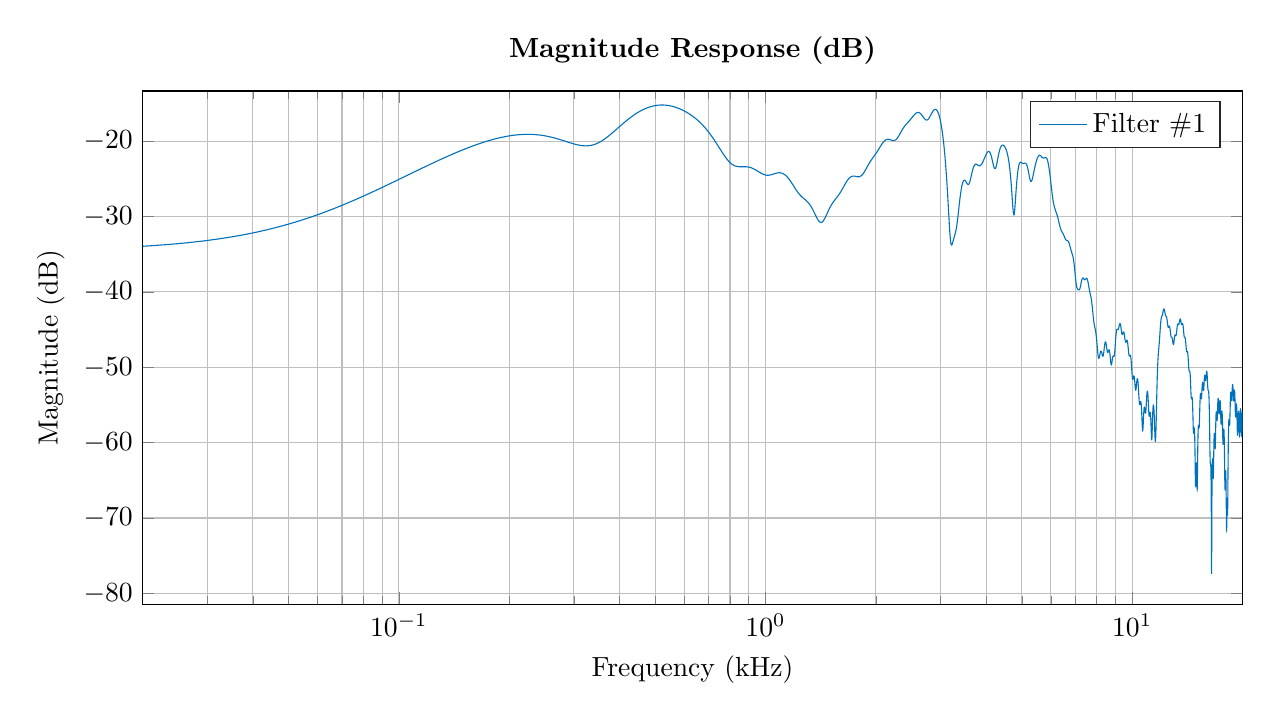
\begin{tikzpicture}

\begin{axis}[%
width=5.5in,
height=2.566in,
at={(1.603in,0.606in)},
scale only axis,
xmode=log,
xmin=0.02,
xmax=20,
xminorticks=true,
xlabel={Frequency (kHz)},
xmajorgrids,
xminorgrids,
ymin=-81.430136633245,
ymax=-13.3444531198088,
ylabel={Magnitude (dB)},
ymajorgrids,
axis background/.style={fill=white},
title style={font=\bfseries},
title={Magnitude Response (dB)},
legend style={legend cell align=left,align=left,draw=white!15!black}
]
\addplot [color=mycolor1,solid,forget plot]
  table[row sep=crcr]{%
0	-34.5938611021637\\
0.0029296875	-34.5799738683775\\
0.005859375	-34.5383451842464\\
0.0087890625	-34.4690814578863\\
0.01171875	-34.3723833560246\\
0.0146484375	-34.2485767604049\\
0.017578125	-34.0981486943751\\
0.0205078125	-33.9217822060783\\
0.0234375	-33.7203842577171\\
0.0263671875	-33.495101685557\\
0.029296875	-33.2473220753311\\
0.0322265625	-32.9786586012721\\
0.03515625	-32.6909200842225\\
0.0380859375	-32.386069339517\\
0.041015625	-32.0661740324772\\
0.0439453125	-31.7333546362495\\
0.046875	-31.3897337635744\\
0.0498046875	-31.037390314381\\
0.052734375	-30.6783207898948\\
0.0556640625	-30.3144090007971\\
0.05859375	-29.9474044121199\\
0.0615234375	-29.5789086161402\\
0.064453125	-29.210368933518\\
0.0673828125	-28.8430778903179\\
0.0703125	-28.478177255564\\
0.0732421875	-28.1166653934147\\
0.076171875	-27.7594068328002\\
0.0791015625	-27.4071431427296\\
0.08203125	-27.0605043929694\\
0.0849609375	-26.7200206581843\\
0.087890625	-26.3861331786537\\
0.0908203125	-26.0592049184745\\
0.09375	-25.739530362994\\
0.0966796875	-25.4273444736738\\
0.099609375	-25.1228307743153\\
0.1025390625	-24.8261285814694\\
0.10546875	-24.5373394175691\\
0.1083984375	-24.2565326610664\\
0.111328125	-23.9837504962794\\
0.1142578125	-23.7190122288775\\
0.1171875	-23.4623180326051\\
0.1201171875	-23.2136521901913\\
0.123046875	-22.9729858873387\\
0.1259765625	-22.7402796138581\\
0.12890625	-22.5154852208909\\
0.1318359375	-22.2985476780266\\
0.134765625	-22.0894065691771\\
0.1376953125	-21.8879973614344\\
0.140625	-21.6942524768716\\
0.1435546875	-21.5081021933685\\
0.146484375	-21.3294753970705\\
0.1494140625	-21.1583002059773\\
0.15234375	-20.9945044814131\\
0.1552734375	-20.8380162416954\\
0.158203125	-20.6887639901767\\
0.1611328125	-20.5466769679499\\
0.1640625	-20.411685339842\\
0.1669921875	-20.2837203208551\\
0.169921875	-20.162714248916\\
0.1728515625	-20.0486006086377\\
0.17578125	-19.9413140097612\\
0.1787109375	-19.8407901230158\\
0.181640625	-19.7469655752823\\
0.1845703125	-19.6597778051639\\
0.1875	-19.5791648793444\\
0.1904296875	-19.5050652694226\\
0.193359375	-19.4374175882657\\
0.1962890625	-19.3761602842918\\
0.19921875	-19.3212312914801\\
0.2021484375	-19.2725676323092\\
0.205078125	-19.2301049702313\\
0.2080078125	-19.1937771077095\\
0.2109375	-19.163515425272\\
0.2138671875	-19.1392482564846\\
0.216796875	-19.1209001932107\\
0.2197265625	-19.1083913150409\\
0.22265625	-19.1016363363463\\
0.2255859375	-19.1005436640716\\
0.228515625	-19.1050143591736\\
0.2314453125	-19.1149409945763\\
0.234375	-19.1302064027154\\
0.2373046875	-19.1506823062662\\
0.240234375	-19.1762278265796\\
0.2431640625	-19.2066878658055\\
0.24609375	-19.2418913608144\\
0.2490234375	-19.281649409976\\
0.251953125	-19.3257532778282\\
0.2548828125	-19.3739722878512\\
0.2578125	-19.4260516201968\\
0.2607421875	-19.4817100395056\\
0.263671875	-19.5406375881046\\
0.2666015625	-19.6024932920625\\
0.26953125	-19.6669029418752\\
0.2724609375	-19.7334570259122\\
0.275390625	-19.8017089129185\\
0.2783203125	-19.8711733993231\\
0.28125	-19.9413257569635\\
0.2841796875	-20.0116014357765\\
0.287109375	-20.0813965921834\\
0.2900390625	-20.1500696249141\\
0.29296875	-20.216943902976\\
0.2958984375	-20.2813118620433\\
0.298828125	-20.3424406223173\\
0.3017578125	-20.399579239705\\
0.3046875	-20.4519676407101\\
0.3076171875	-20.498847208998\\
0.310546875	-20.5394728897794\\
0.3134765625	-20.5731265615323\\
0.31640625	-20.5991313010443\\
0.3193359375	-20.6168660484196\\
0.322265625	-20.6257800770828\\
0.3251953125	-20.625406604326\\
0.328125	-20.6153748537554\\
0.3310546875	-20.5954199115661\\
0.333984375	-20.5653898074495\\
0.3369140625	-20.5252493942374\\
0.33984375	-20.4750807865532\\
0.3427734375	-20.4150803297941\\
0.345703125	-20.345552284825\\
0.3486328125	-20.2668996084834\\
0.3515625	-20.1796123660642\\
0.3544921875	-20.0842544159304\\
0.357421875	-19.9814490523423\\
0.3603515625	-19.8718642821899\\
0.36328125	-19.7561983526409\\
0.3662109375	-19.6351660522172\\
0.369140625	-19.5094861917825\\
0.3720703125	-19.3798705482976\\
0.375	-19.2470144348433\\
0.3779296875	-19.1115889540944\\
0.380859375	-18.9742349046031\\
0.3837890625	-18.835558242235\\
0.38671875	-18.6961269527155\\
0.3896484375	-18.5564691635418\\
0.392578125	-18.4170723115133\\
0.3955078125	-18.2783831824123\\
0.3984375	-18.1408086485609\\
0.4013671875	-18.0047169450546\\
0.404296875	-17.8704393438892\\
0.4072265625	-17.7382721049726\\
0.41015625	-17.6084786026848\\
0.4130859375	-17.481291545232\\
0.416015625	-17.3569152209211\\
0.4189453125	-17.2355277203458\\
0.421875	-17.1172830962319\\
0.4248046875	-17.0023134333841\\
0.427734375	-16.8907308099618\\
0.4306640625	-16.7826291383744\\
0.43359375	-16.6780858796591\\
0.4365234375	-16.5771636295003\\
0.439453125	-16.4799115772822\\
0.4423828125	-16.3863668419258\\
0.4453125	-16.2965556899206\\
0.4482421875	-16.2104946420584\\
0.451171875	-16.128191476042\\
0.4541015625	-16.049646132474\\
0.45703125	-15.9748515318083\\
0.4599609375	-15.9037943097492\\
0.462890625	-15.8364554783466\\
0.4658203125	-15.7728110197187\\
0.46875	-15.7128324189542\\
0.4716796875	-15.6564871423396\\
0.474609375	-15.6037390666341\\
0.4775390625	-15.5545488646928\\
0.48046875	-15.5088743523261\\
0.4833984375	-15.4666708008861\\
0.486328125	-15.4278912196921\\
0.4892578125	-15.3924866120539\\
0.4921875	-15.3604062083151\\
0.4951171875	-15.3315976790325\\
0.498046875	-15.3060073311174\\
0.5009765625	-15.2835802894975\\
0.50390625	-15.2642606666132\\
0.5068359375	-15.2479917218288\\
0.509765625	-15.234716012629\\
0.5126953125	-15.2243755392685\\
0.515625	-15.2169118843579\\
0.5185546875	-15.21226634869\\
0.521484375	-15.2103800844479\\
0.5244140625	-15.2111942267717\\
0.52734375	-15.2146500245125\\
0.5302734375	-15.2206889708535\\
0.533203125	-15.2292529343359\\
0.5361328125	-15.2402842906895\\
0.5390625	-15.2537260557341\\
0.5419921875	-15.2695220194844\\
0.544921875	-15.2876168814683\\
0.5478515625	-15.3079563871378\\
0.55078125	-15.3304874651374\\
0.5537109375	-15.3551583650753\\
0.556640625	-15.3819187953329\\
0.5595703125	-15.4107200603427\\
0.5625	-15.4415151966667\\
0.5654296875	-15.4742591071139\\
0.568359375	-15.508908692058\\
0.5712890625	-15.5454229770373\\
0.57421875	-15.5837632356614\\
0.5771484375	-15.6238931067966\\
0.580078125	-15.6657787049623\\
0.5830078125	-15.7093887228471\\
0.5859375	-15.7546945248383\\
0.5888671875	-15.8016702304616\\
0.591796875	-15.850292786639\\
0.5947265625	-15.9005420277053\\
0.59765625	-15.9524007221561\\
0.6005859375	-16.0058546051598\\
0.603515625	-16.0608923959195\\
0.6064453125	-16.1175057990492\\
0.609375	-16.1756894891997\\
0.6123046875	-16.2354410782568\\
0.615234375	-16.2967610645201\\
0.6181640625	-16.3596527633568\\
0.62109375	-16.4241222189107\\
0.6240234375	-16.4901780965315\\
0.626953125	-16.5578315556627\\
0.6298828125	-16.6270961029966\\
0.6328125	-16.6979874257646\\
0.6357421875	-16.7705232050743\\
0.638671875	-16.8447229092434\\
0.6416015625	-16.9206075670958\\
0.64453125	-16.9981995211923\\
0.6474609375	-17.0775221609583\\
0.650390625	-17.158599635643\\
0.6533203125	-17.2414565470081\\
0.65625	-17.3261176215888\\
0.6591796875	-17.4126073623105\\
0.662109375	-17.5009496791664\\
0.6650390625	-17.5911674985922\\
0.66796875	-17.6832823510888\\
0.6708984375	-17.777313936575\\
0.673828125	-17.8732796668832\\
0.6767578125	-17.9711941847645\\
0.6796875	-18.071068858745\\
0.6826171875	-18.1729112531798\\
0.685546875	-18.2767245729073\\
0.6884765625	-18.382507082009\\
0.69140625	-18.4902514963576\\
0.6943359375	-18.5999443498931\\
0.697265625	-18.7115653349267\\
0.7001953125	-18.8250866172506\\
0.703125	-18.9404721274459\\
0.7060546875	-19.0576768305596\\
0.708984375	-19.1766459772788\\
0.7119140625	-19.2973143408913\\
0.71484375	-19.4196054457096\\
0.7177734375	-19.5434307942639\\
0.720703125	-19.6686891024563\\
0.7236328125	-19.7952655540199\\
0.7265625	-19.9230310880336\\
0.7294921875	-20.0518417359\\
0.732421875	-20.1815380270479\\
0.7353515625	-20.3119444856306\\
0.73828125	-20.4428692435492\\
0.7412109375	-20.5741037981275\\
0.744140625	-20.7054229455359\\
0.7470703125	-20.8365849233941\\
0.75	-20.9673317976442\\
0.7529296875	-21.09739012948\\
0.755859375	-21.2264719575257\\
0.7587890625	-21.3542761282555\\
0.76171875	-21.4804900034819\\
0.7646484375	-21.6047915673375\\
0.767578125	-21.7268519462929\\
0.7705078125	-21.8463383442812\\
0.7734375	-21.9629173810015\\
0.7763671875	-22.0762588051809\\
0.779296875	-22.1860395365133\\
0.7822265625	-22.2919479709066\\
0.78515625	-22.3936884645784\\
0.7880859375	-22.4909858946858\\
0.791015625	-22.583590178927\\
0.7939453125	-22.6712806253361\\
0.796875	-22.7538699776178\\
0.7998046875	-22.8312080218939\\
0.802734375	-22.9031846283231\\
0.8056640625	-22.9697321158404\\
0.80859375	-23.0308268497827\\
0.8115234375	-23.0864900093582\\
0.814453125	-23.1367874931808\\
0.8173828125	-23.1818289644287\\
0.8203125	-23.221766070381\\
0.8232421875	-23.2567899019658\\
0.826171875	-23.2871277855319\\
0.8291015625	-23.31303951981\\
0.83203125	-23.3348131849608\\
0.8349609375	-23.3527606573191\\
0.837890625	-23.3672129631545\\
0.8408203125	-23.3785155981791\\
0.84375	-23.3870239277535\\
0.8466796875	-23.3930987670994\\
0.849609375	-23.3971022227476\\
0.8525390625	-23.3993938572972\\
0.85546875	-23.4003272205565\\
0.8583984375	-23.400246772261\\
0.861328125	-23.3994852055566\\
0.8642578125	-23.3983611667641\\
0.8671875	-23.3971773558421\\
0.8701171875	-23.396218983465\\
0.873046875	-23.3957525546181\\
0.8759765625	-23.3960249448351\\
0.87890625	-23.3972627333836\\
0.8818359375	-23.3996717574984\\
0.884765625	-23.4034368528518\\
0.8876953125	-23.4087217475212\\
0.890625	-23.4156690794969\\
0.8935546875	-23.4244005110251\\
0.896484375	-23.4350169166215\\
0.8994140625	-23.44759862526\\
0.90234375	-23.4622057009287\\
0.9052734375	-23.4788782493746\\
0.908203125	-23.4976367423707\\
0.9111328125	-23.5184823541972\\
0.9140625	-23.5413973082235\\
0.9169921875	-23.5663452344825\\
0.919921875	-23.5932715419516\\
0.9228515625	-23.6221038118705\\
0.92578125	-23.6527522208418\\
0.9287109375	-23.6851100046311\\
0.931640625	-23.7190539755027\\
0.9345703125	-23.7544451075296\\
0.9375	-23.7911292055637\\
0.9404296875	-23.8289376743614\\
0.943359375	-23.8676884046609\\
0.9462890625	-23.9071867927042\\
0.94921875	-23.9472269086991\\
0.9521484375	-23.9875928279404\\
0.955078125	-24.0280601356617\\
0.9580078125	-24.0683976131322\\
0.9609375	-24.1083691080014\\
0.9638671875	-24.1477355864659\\
0.966796875	-24.1862573585471\\
0.9697265625	-24.2236964607781\\
0.97265625	-24.259819173111\\
0.9755859375	-24.2943986391559\\
0.978515625	-24.3272175513086\\
0.9814453125	-24.3580708553236\\
0.984375	-24.3867684228802\\
0.9873046875	-24.4131376361296\\
0.990234375	-24.4370258255081\\
0.9931640625	-24.4583025016104\\
0.99609375	-24.4768613238828\\
0.9990234375	-24.4926217534162\\
1.001953125	-24.5055303441409\\
1.0048828125	-24.5155616360209\\
1.0078125	-24.5227186250098\\
1.0107421875	-24.5270327970393\\
1.013671875	-24.5285637265062\\
1.0166015625	-24.5273982529177\\
1.01953125	-24.5236492618484\\
1.0224609375	-24.5174541074999\\
1.025390625	-24.5089727234293\\
1.0283203125	-24.4983854749948\\
1.03125	-24.4858908115643\\
1.0341796875	-24.4717027784686\\
1.037109375	-24.4560484481687\\
1.0400390625	-24.4391653273973\\
1.04296875	-24.4212987924663\\
1.0458984375	-24.4026995989362\\
1.048828125	-24.3836215048559\\
1.0517578125	-24.3643190392503\\
1.0546875	-24.3450454398628\\
1.0576171875	-24.3260507766952\\
1.060546875	-24.307580270926\\
1.0634765625	-24.2898728125152\\
1.06640625	-24.2731596743762\\
1.0693359375	-24.2576634164702\\
1.072265625	-24.2435969695676\\
1.0751953125	-24.2311628857066\\
1.078125	-24.220552740469\\
1.0810546875	-24.2119466710296\\
1.083984375	-24.2055130333924\\
1.0869140625	-24.2014081622148\\
1.08984375	-24.1997762170304\\
1.0927734375	-24.2007490994213\\
1.095703125	-24.2044464266714\\
1.0986328125	-24.2109755485829\\
1.1015625	-24.2204315953994\\
1.1044921875	-24.2328975460981\\
1.107421875	-24.2484443076528\\
1.1103515625	-24.2671307972108\\
1.11328125	-24.2890040204376\\
1.1162109375	-24.3140991405729\\
1.119140625	-24.3424395339849\\
1.1220703125	-24.3740368292322\\
1.125	-24.4088909278292\\
1.1279296875	-24.4469900060845\\
1.130859375	-24.4883104985455\\
1.1337890625	-24.5328170647476\\
1.13671875	-24.5804625421498\\
1.1396484375	-24.6311878893347\\
1.142578125	-24.6849221247859\\
1.1455078125	-24.7415822678098\\
1.1484375	-24.8010732894612\\
1.1513671875	-24.8632880826335\\
1.154296875	-24.9281074617871\\
1.1572265625	-24.9954002040707\\
1.16015625	-25.0650231448215\\
1.1630859375	-25.1368213415513\\
1.166015625	-25.2106283214841\\
1.1689453125	-25.2862664284388\\
1.171875	-25.3635472852596\\
1.1748046875	-25.4422723880018\\
1.177734375	-25.5222338475778\\
1.1806640625	-25.6032152934616\\
1.18359375	-25.6849929522372\\
1.1865234375	-25.7673369111759\\
1.189453125	-25.8500125735701\\
1.1923828125	-25.9327823082081\\
1.1953125	-26.0154072901466\\
1.1982421875	-26.0976495238995\\
1.201171875	-26.1792740334234\\
1.2041015625	-26.2600511960559\\
1.20703125	-26.3397591900955\\
1.2099609375	-26.4181865183615\\
1.212890625	-26.4951345631972\\
1.2158203125	-26.5704201224299\\
1.21875	-26.6438778711889\\
1.2216796875	-26.7153626916246\\
1.224609375	-26.7847518118146\\
1.2275390625	-26.8519466967235\\
1.23046875	-26.9168746381412\\
1.2333984375	-26.9794899969992\\
1.236328125	-27.0397750601794\\
1.2392578125	-27.0977404845067\\
1.2421875	-27.1534253125661\\
1.2451171875	-27.2068965576835\\
1.248046875	-27.2582483682034\\
1.2509765625	-27.3076007933961\\
1.25390625	-27.3550981843005\\
1.2568359375	-27.4009072720313\\
1.259765625	-27.4452149731277\\
1.2626953125	-27.4882259761648\\
1.265625	-27.5301601659971\\
1.2685546875	-27.5712499417305\\
1.271484375	-27.6117374820513\\
1.2744140625	-27.6518720071818\\
1.27734375	-27.6919070808908\\
1.2802734375	-27.7320979890874\\
1.283203125	-27.7726992239933\\
1.2861328125	-27.8139620951333\\
1.2890625	-27.8561324807566\\
1.2919921875	-27.8994487260881\\
1.294921875	-27.9441396882449\\
1.2978515625	-27.9904229218828\\
1.30078125	-28.038502994762\\
1.3037109375	-28.0885699184819\\
1.306640625	-28.1407976766297\\
1.3095703125	-28.1953428305035\\
1.3125	-28.2523431813473\\
1.3154296875	-28.3119164676564\\
1.318359375	-28.3741590765114\\
1.3212890625	-28.4391447490777\\
1.32421875	-28.5069232623505\\
1.3271484375	-28.5775190719631\\
1.330078125	-28.6509299044627\\
1.3330078125	-28.7271252919679\\
1.3359375	-28.8060450476773\\
1.3388671875	-28.8875976874118\\
1.341796875	-28.971658810396\\
1.3447265625	-29.0580694619492\\
1.34765625	-29.146634511763\\
1.3505859375	-29.2371210940586\\
1.353515625	-29.3292571700811\\
1.3564453125	-29.4227302889288\\
1.359375	-29.5171866392311\\
1.3623046875	-29.6122305010298\\
1.365234375	-29.7074242234042\\
1.3681640625	-29.8022888675303\\
1.37109375	-29.8963056652073\\
1.3740234375	-29.9889184472224\\
1.376953125	-30.0795371917438\\
1.3798828125	-30.1675428275693\\
1.3828125	-30.2522933979592\\
1.3857421875	-30.3331316459261\\
1.388671875	-30.4093940202402\\
1.3916015625	-30.480421023611\\
1.39453125	-30.5455687331946\\
1.3974609375	-30.6042212239022\\
1.400390625	-30.6558035246093\\
1.4033203125	-30.6997946461248\\
1.40625	-30.7357401487575\\
1.4091796875	-30.7632636774747\\
1.412109375	-30.7820768930664\\
1.4150390625	-30.7919872738268\\
1.41796875	-30.7929033543398\\
1.4208984375	-30.784837100452\\
1.423828125	-30.7679032812836\\
1.4267578125	-30.7423158747589\\
1.4296875	-30.7083817151463\\
1.4326171875	-30.6664917425504\\
1.435546875	-30.6171103312957\\
1.4384765625	-30.5607632477456\\
1.44140625	-30.4980248151571\\
1.4443359375	-30.4295048462363\\
1.447265625	-30.3558358502416\\
1.4501953125	-30.2776609408593\\
1.453125	-30.1956227748595\\
1.4560546875	-30.1103537504355\\
1.458984375	-30.0224675971638\\
1.4619140625	-29.9325524033507\\
1.46484375	-29.8411650552393\\
1.4677734375	-29.74882700792\\
1.470703125	-29.6560212696444\\
1.4736328125	-29.5631904581346\\
1.4765625	-29.4707357770708\\
1.4794921875	-29.3790167606203\\
1.482421875	-29.2883516409776\\
1.4853515625	-29.1990182060295\\
1.48828125	-29.1112550293983\\
1.4912109375	-29.0252629716304\\
1.494140625	-28.9412068679679\\
1.4970703125	-28.8592173341187\\
1.5	-28.7793926361713\\
1.5029296875	-28.7018005839716\\
1.505859375	-28.6264804187614\\
1.5087890625	-28.5534446756533\\
1.51171875	-28.4826810096617\\
1.5146484375	-28.4141539806272\\
1.517578125	-28.3478067976158\\
1.5205078125	-28.283563027367\\
1.5234375	-28.2213282742469\\
1.5263671875	-28.1609918410581\\
1.529296875	-28.1024283810569\\
1.5322265625	-28.0454995517331\\
1.53515625	-27.9900556803836\\
1.5380859375	-27.9359374503307\\
1.541015625	-27.8829776148597\\
1.5439453125	-27.8310027436453\\
1.546875	-27.7798350036649\\
1.5498046875	-27.7292939734547\\
1.552734375	-27.6791984861284\\
1.5556640625	-27.6293684929785\\
1.55859375	-27.579626935832\\
1.5615234375	-27.529801612792\\
1.564453125	-27.4797270187113\\
1.5673828125	-27.4292461388864\\
1.5703125	-27.3782121721865\\
1.5732421875	-27.326490158289\\
1.576171875	-27.2739584830194\\
1.5791015625	-27.2205102360673\\
1.58203125	-27.1660543966404\\
1.5849609375	-27.1105168249179\\
1.587890625	-27.0538410404197\\
1.5908203125	-26.9959887725269\\
1.59375	-26.9369402731949\\
1.5966796875	-26.8766943872133\\
1.599609375	-26.815268380942\\
1.6025390625	-26.7526975360537\\
1.60546875	-26.6890345201841\\
1.6083984375	-26.6243485513093\\
1.611328125	-26.5587243769237\\
1.6142578125	-26.4922610925321\\
1.6171875	-26.4250708264775\\
1.6201171875	-26.3572773196568\\
1.623046875	-26.2890144292159\\
1.6259765625	-26.220424584926\\
1.62890625	-26.1516572257066\\
1.6318359375	-26.0828672417986\\
1.634765625	-26.0142134455631\\
1.6376953125	-25.9458570909208\\
1.640625	-25.8779604582342\\
1.6435546875	-25.8106855180986\\
1.646484375	-25.7441926841939\\
1.6494140625	-25.678639662165\\
1.65234375	-25.614180398536\\
1.6552734375	-25.5509641309911\\
1.658203125	-25.4891345390153\\
1.6611328125	-25.4288289919097\\
1.6640625	-25.3701778895793\\
1.6669921875	-25.3133040902319\\
1.669921875	-25.2583224182077\\
1.6728515625	-25.2053392445447\\
1.67578125	-25.1544521325531\\
1.6787109375	-25.1057495405792\\
1.681640625	-25.0593105742561\\
1.6845703125	-25.0152047808304\\
1.6875	-24.9734919785856\\
1.6904296875	-24.9342221149339\\
1.693359375	-24.8974351473867\\
1.6962890625	-24.8631609423281\\
1.69921875	-24.8314191872804\\
1.7021484375	-24.8022193131602\\
1.705078125	-24.7755604238681\\
1.7080078125	-24.7514312314217\\
1.7109375	-24.729809995732\\
1.7138671875	-24.7106644690317\\
1.716796875	-24.6939518458873\\
1.7197265625	-24.6796187206619\\
1.72265625	-24.6676010552387\\
1.7255859375	-24.6578241607664\\
1.728515625	-24.6502026981289\\
1.7314453125	-24.6446407027708\\
1.734375	-24.6410316404142\\
1.7373046875	-24.6392585010488\\
1.740234375	-24.6391939393645\\
1.7431640625	-24.640700470466\\
1.74609375	-24.6436307302563\\
1.7490234375	-24.6478278102356\\
1.751953125	-24.6531256766003\\
1.7548828125	-24.6593496833967\\
1.7578125	-24.6663171890241\\
1.7607421875	-24.6738382845497\\
1.763671875	-24.6817166410472\\
1.7666015625	-24.6897504814555\\
1.76953125	-24.6977336802575\\
1.7724609375	-24.7054569915817\\
1.775390625	-24.7127094031557\\
1.7783203125	-24.7192796099216\\
1.78125	-24.7249575971362\\
1.7841796875	-24.7295363185297\\
1.787109375	-24.7328134507227\\
1.7900390625	-24.7345932007759\\
1.79296875	-24.7346881396721\\
1.7958984375	-24.7329210309206\\
1.798828125	-24.7291266205493\\
1.8017578125	-24.7231533527414\\
1.8046875	-24.7148649744516\\
1.8076171875	-24.7041419926704\\
1.810546875	-24.6908829496774\\
1.8134765625	-24.6750054846669\\
1.81640625	-24.6564471544782\\
1.8193359375	-24.6351659917016\\
1.822265625	-24.6111407849334\\
1.8251953125	-24.5843710731552\\
1.828125	-24.5548768537928\\
1.8310546875	-24.5226980116145\\
1.833984375	-24.487893482918\\
1.8369140625	-24.4505401760904\\
1.83984375	-24.4107316753383\\
1.8427734375	-24.3685767589425\\
1.845703125	-24.3241977666611\\
1.8486328125	-24.2777288528108\\
1.8515625	-24.2293141621174\\
1.8544921875	-24.1791059647302\\
1.857421875	-24.1272627849721\\
1.8603515625	-24.0739475556538\\
1.86328125	-24.0193258263076\\
1.8662109375	-23.9635640497382\\
1.869140625	-23.9068279670477\\
1.8720703125	-23.8492811069818\\
1.875	-23.791083411238\\
1.8779296875	-23.7323899934123\\
1.880859375	-23.673350035662\\
1.8837890625	-23.6141058239911\\
1.88671875	-23.5547919203711\\
1.8896484375	-23.4955344677153\\
1.892578125	-23.4364506220037\\
1.8955078125	-23.3776481046054\\
1.8984375	-23.3192248670046\\
1.9013671875	-23.2612688596654\\
1.904296875	-23.2038578966217\\
1.9072265625	-23.1470596074803\\
1.91015625	-23.0909314688402\\
1.9130859375	-23.0355209075942\\
1.916015625	-22.9808654691569\\
1.9189453125	-22.9269930442925\\
1.921875	-22.8739221488915\\
1.9248046875	-22.8216622516969\\
1.927734375	-22.770214145621\\
1.9306640625	-22.7195703588676\\
1.93359375	-22.6697156025899\\
1.9365234375	-22.6206272522438\\
1.939453125	-22.5722758601339\\
1.9423828125	-22.5246256968972\\
1.9453125	-22.4776353198088\\
1.9482421875	-22.4312581658422\\
1.951171875	-22.3854431673646\\
1.9541015625	-22.3401353882089\\
1.95703125	-22.2952766776368\\
1.9599609375	-22.2508063394173\\
1.962890625	-22.2066618128904\\
1.9658203125	-22.1627793624879\\
1.96875	-22.1190947717649\\
1.9716796875	-22.075544037564\\
1.974609375	-22.0320640595169\\
1.9775390625	-21.9885933197078\\
1.98046875	-21.9450725469915\\
1.9833984375	-21.9014453602039\\
1.986328125	-21.8576588843388\\
1.9892578125	-21.8136643337116\\
1.9921875	-21.7694175561917\\
1.9951171875	-21.7248795327854\\
1.998046875	-21.6800168271773\\
2.0009765625	-21.634801980304\\
2.00390625	-21.5892138456261\\
2.0068359375	-21.5432378614734\\
2.009765625	-21.4968662576537\\
2.0126953125	-21.450098194409\\
2.015625	-21.4029398327584\\
2.0185546875	-21.3554043362553\\
2.021484375	-21.3075118051778\\
2.0244140625	-21.2592891451453\\
2.02734375	-21.2107698730725\\
2.0302734375	-21.1619938642214\\
2.033203125	-21.1130070448591\\
2.0361328125	-21.0638610356688\\
2.0390625	-21.0146127515654\\
2.0419921875	-20.9653239639389\\
2.044921875	-20.9160608315794\\
2.0478515625	-20.8668934066271\\
2.05078125	-20.8178951218483\\
2.0537109375	-20.7691422653716\\
2.056640625	-20.7207134487394\\
2.0595703125	-20.6726890737581\\
2.0625	-20.6251508031755\\
2.0654296875	-20.578181039705\\
2.068359375	-20.5318624173566\\
2.0712890625	-20.4862773084582\\
2.07421875	-20.44150734916\\
2.0771484375	-20.3976329856334\\
2.080078125	-20.3547330426126\\
2.0830078125	-20.312884315394\\
2.0859375	-20.2721611859176\\
2.0888671875	-20.2326352631032\\
2.091796875	-20.1943750472238\\
2.0947265625	-20.157445617749\\
2.09765625	-20.1219083438129\\
2.1005859375	-20.0878206162207\\
2.103515625	-20.0552355997372\\
2.1064453125	-20.0242020042731\\
2.109375	-19.99476387351\\
2.1123046875	-19.9669603894779\\
2.115234375	-19.9408256916144\\
2.1181640625	-19.9163887088912\\
2.12109375	-19.8936730036885\\
2.1240234375	-19.8726966262229\\
2.126953125	-19.8534719784988\\
2.1298828125	-19.8360056869365\\
2.1328125	-19.8202984830502\\
2.1357421875	-19.8063450917833\\
2.138671875	-19.7941341273746\\
2.1416015625	-19.7836479969064\\
2.14453125	-19.774862811989\\
2.1474609375	-19.7677483093485\\
2.150390625	-19.7622677814179\\
2.1533203125	-19.7583780183673\\
2.15625	-19.7560292633602\\
2.1591796875	-19.7551651831698\\
2.162109375	-19.7557228566373\\
2.1650390625	-19.7576327837937\\
2.16796875	-19.7608189187866\\
2.1708984375	-19.7651987300506\\
2.173828125	-19.7706832914212\\
2.1767578125	-19.7771774081014\\
2.1796875	-19.7845797815444\\
2.1826171875	-19.7927832173879\\
2.185546875	-19.80167488056\\
2.1884765625	-19.8111366015528\\
2.19140625	-19.8210452376105\\
2.1943359375	-19.8312730921916\\
2.197265625	-19.8416883955269\\
2.2001953125	-19.8521558483864\\
2.203125	-19.8625372302988\\
2.2060546875	-19.8726920724126\\
2.208984375	-19.8824783939763\\
2.2119140625	-19.8917535000334\\
2.21484375	-19.9003748364215\\
2.2177734375	-19.9082008965412\\
2.220703125	-19.9150921726708\\
2.2236328125	-19.9209121428962\\
2.2265625	-19.9255282830489\\
2.2294921875	-19.9288130914736\\
2.232421875	-19.9306451130385\\
2.2353515625	-19.9309099476376\\
2.23828125	-19.9295012275668\\
2.2412109375	-19.9263215476637\\
2.244140625	-19.9212833320208\\
2.2470703125	-19.9143096214622\\
2.25	-19.9053347668252\\
2.2529296875	-19.8943050144184\\
2.255859375	-19.8811789718031\\
2.2587890625	-19.8659279442361\\
2.26171875	-19.8485361346338\\
2.2646484375	-19.8290007027042\\
2.267578125	-19.8073316818388\\
2.2705078125	-19.7835517553493\\
2.2734375	-19.7576958965787\\
2.2763671875	-19.7298108801922\\
2.279296875	-19.6999546744748\\
2.2822265625	-19.668195726635\\
2.28515625	-19.6346121548855\\
2.2880859375	-19.5992908623867\\
2.291015625	-19.5623265889817\\
2.2939453125	-19.523820917021\\
2.296875	-19.483881247491\\
2.2998046875	-19.4426197621589\\
2.302734375	-19.4001523865857\\
2.3056640625	-19.3565977676895\\
2.30859375	-19.3120762781456\\
2.3115234375	-19.2667090583421\\
2.314453125	-19.2206171049525\\
2.3173828125	-19.1739204134895\\
2.3203125	-19.126737180538\\
2.3232421875	-19.079183069761\\
2.326171875	-19.0313705442863\\
2.3291015625	-18.9834082667287\\
2.33203125	-18.9354005669084\\
2.3349609375	-18.8874469763038\\
2.337890625	-18.8396418274241\\
2.3408203125	-18.7920739156058\\
2.34375	-18.744826220219\\
2.3466796875	-18.6979756818978\\
2.349609375	-18.6515930321791\\
2.3525390625	-18.6057426718182\\
2.35546875	-18.5604825940402\\
2.3583984375	-18.5158643490611\\
2.361328125	-18.471933046359\\
2.3642578125	-18.4287273913703\\
2.3671875	-18.3862797535284\\
2.3701171875	-18.3446162628243\\
2.373046875	-18.3037569323454\\
2.3759765625	-18.2637158045368\\
2.37890625	-18.2245011192044\\
2.3818359375	-18.1861155015469\\
2.384765625	-18.1485561687562\\
2.3876953125	-18.1118151539468\\
2.390625	-18.0758795463767\\
2.3935546875	-18.0407317470899\\
2.396484375	-18.0063497392441\\
2.3994140625	-17.9727073724884\\
2.40234375	-17.9397746608207\\
2.4052734375	-17.9075180933805\\
2.408203125	-17.8759009576294\\
2.4111328125	-17.8448836743234\\
2.4140625	-17.8144241436124\\
2.4169921875	-17.7844781014905\\
2.419921875	-17.7549994856878\\
2.4228515625	-17.7259408099371\\
2.42578125	-17.6972535453672\\
2.4287109375	-17.6688885075813\\
2.431640625	-17.6407962477753\\
2.4345703125	-17.6129274460413\\
2.4375	-17.5852333047971\\
2.4404296875	-17.5576659400883\\
2.443359375	-17.5301787683268\\
2.4462890625	-17.5027268858771\\
2.44921875	-17.4752674387743\\
2.4521484375	-17.4477599797686\\
2.455078125	-17.4201668098425\\
2.4580078125	-17.3924533013486\\
2.4609375	-17.3645881999619\\
2.4638671875	-17.3365439027444\\
2.466796875	-17.3082967097725\\
2.4697265625	-17.2798270469864\\
2.47265625	-17.2511196581781\\
2.4755859375	-17.2221637643346\\
2.478515625	-17.1929531889009\\
2.4814453125	-17.1634864479023\\
2.484375	-17.1337668042684\\
2.4873046875	-17.1038022861225\\
2.490234375	-17.0736056692271\\
2.4931640625	-17.0431944241984\\
2.49609375	-17.0125906295189\\
2.4990234375	-16.981820851764\\
2.501953125	-16.950915994822\\
2.5048828125	-16.9199111202064\\
2.5078125	-16.8888452408412\\
2.5107421875	-16.8577610909256\\
2.513671875	-16.8267048746637\\
2.5166015625	-16.795725996766\\
2.51953125	-16.7648767776968\\
2.5224609375	-16.7342121566558\\
2.525390625	-16.7037893852455\\
2.5283203125	-16.673667714692\\
2.53125	-16.6439080793579\\
2.5341796875	-16.6145727791259\\
2.537109375	-16.5857251630321\\
2.5400390625	-16.5574293163114\\
2.54296875	-16.5297497527764\\
2.5458984375	-16.5027511142006\\
2.548828125	-16.4764978781192\\
2.5517578125	-16.4510540752\\
2.5546875	-16.4264830170845\\
2.5576171875	-16.4028470353487\\
2.560546875	-16.3802072319999\\
2.5634765625	-16.3586232417064\\
2.56640625	-16.3381530057496\\
2.5693359375	-16.3188525575085\\
2.572265625	-16.3007758191202\\
2.5751953125	-16.2839744088171\\
2.578125	-16.2684974583211\\
2.5810546875	-16.2543914395727\\
2.583984375	-16.2416999999961\\
2.5869140625	-16.230463805439\\
2.58984375	-16.2207203898892\\
2.5927734375	-16.2125040110457\\
2.595703125	-16.2058455108235\\
2.5986328125	-16.2007721798822\\
2.6015625	-16.1973076253013\\
2.6044921875	-16.1954716405729\\
2.607421875	-16.1952800771437\\
2.6103515625	-16.1967447168196\\
2.61328125	-16.1998731444363\\
2.6162109375	-16.2046686203124\\
2.619140625	-16.2111299521239\\
2.6220703125	-16.2192513659829\\
2.625	-16.2290223766576\\
2.6279296875	-16.2404276570504\\
2.630859375	-16.2534469072416\\
2.6337890625	-16.2680547236183\\
2.63671875	-16.2842204688395\\
2.6396484375	-16.3019081436402\\
2.642578125	-16.3210762617434\\
2.6455078125	-16.3416777294417\\
2.6484375	-16.3636597317148\\
2.6513671875	-16.3869636270706\\
2.654296875	-16.4115248536375\\
2.6572265625	-16.4372728493773\\
2.66015625	-16.4641309896407\\
2.6630859375	-16.4920165456365\\
2.666015625	-16.5208406677216\\
2.6689453125	-16.5505083977378\\
2.671875	-16.5809187149093\\
2.6748046875	-16.6119646200511\\
2.677734375	-16.6435332630173\\
2.6806640625	-16.6755061184191\\
2.68359375	-16.7077592146372\\
2.6865234375	-16.7401634210366\\
2.689453125	-16.7725847980333\\
2.6923828125	-16.8048850142429\\
2.6953125	-16.8369218343456\\
2.6982421875	-16.8685496805149\\
2.701171875	-16.8996202692636\\
2.7041015625	-16.9299833243556\\
2.70703125	-16.9594873650287\\
2.7099609375	-16.9879805671612\\
2.712890625	-17.0153116932434\\
2.7158203125	-17.0413310850927\\
2.71875	-17.0658917112426\\
2.7216796875	-17.0888502588867\\
2.724609375	-17.1100682582469\\
2.7275390625	-17.1294132253316\\
2.73046875	-17.1467598073447\\
2.7333984375	-17.1619909135819\\
2.736328125	-17.174998813597\\
2.7392578125	-17.185686183809\\
2.7421875	-17.1939670836221\\
2.7451171875	-17.1997678425858\\
2.748046875	-17.203027841161\\
2.7509765625	-17.2037001692703\\
2.75390625	-17.2017521489812\\
2.7568359375	-17.1971657103196\\
2.759765625	-17.189937612278\\
2.7626953125	-17.1800795044417\\
2.765625	-17.1676178281891\\
2.7685546875	-17.1525935600064\\
2.771484375	-17.1350618029293\\
2.7744140625	-17.1150912353868\\
2.77734375	-17.0927634296274\\
2.7802734375	-17.0681720543779\\
2.783203125	-17.0414219783321\\
2.7861328125	-17.0126282924555\\
2.7890625	-16.9819152698914\\
2.7919921875	-16.9494152824822\\
2.794921875	-16.915267692612\\
2.7978515625	-16.8796177382706\\
2.80078125	-16.8426154280338\\
2.8037109375	-16.8044144611005\\
2.806640625	-16.7651711857352\\
2.8095703125	-16.7250436075028\\
2.8125	-16.6841904566468\\
2.8154296875	-16.6427703219207\\
2.818359375	-16.6009408561957\\
2.8212890625	-16.558858057304\\
2.82421875	-16.5166756258554\\
2.8271484375	-16.4745444002384\\
2.830078125	-16.432611867681\\
2.8330078125	-16.3910217491249\\
2.8359375	-16.3499136547517\\
2.8388671875	-16.3094228062805\\
2.841796875	-16.2696798216302\\
2.8447265625	-16.2308105571777\\
2.84765625	-16.1929360026305\\
2.8505859375	-16.1561722234587\\
2.853515625	-16.1206303458537\\
2.8564453125	-16.0864165793041\\
2.859375	-16.0536322720691\\
2.8623046875	-16.0223739950695\\
2.865234375	-15.9927336500047\\
2.8681640625	-15.9647985978061\\
2.87109375	-15.9386518038642\\
2.8740234375	-15.9143719967896\\
2.876953125	-15.8920338377952\\
2.8798828125	-15.8717080981015\\
2.8828125	-15.853461842068\\
2.8857421875	-15.8373586140415\\
2.888671875	-15.8234586271768\\
2.8916015625	-15.8118189527358\\
2.89453125	-15.8024937085913\\
2.8974609375	-15.795534245875\\
2.900390625	-15.7909893328873\\
2.9033203125	-15.7889053355554\\
2.90625	-15.7893263938746\\
2.9091796875	-15.792294593893\\
2.912109375	-15.7978501349172\\
2.9150390625	-15.8060314917122\\
2.91796875	-15.8168755715567\\
2.9208984375	-15.8304178660823\\
2.923828125	-15.8466925978943\\
2.9267578125	-15.865732862016\\
2.9296875	-15.8875707622468\\
2.9326171875	-15.9122375425563\\
2.935546875	-15.9397637136677\\
2.9384765625	-15.9701791750041\\
2.94140625	-16.0035133321907\\
2.9443359375	-16.0397952103175\\
2.947265625	-16.0790535631773\\
2.9501953125	-16.1213169786984\\
2.953125	-16.1666139807963\\
2.9560546875	-16.2149731278673\\
2.958984375	-16.2664231081473\\
2.9619140625	-16.3209928321544\\
2.96484375	-16.3787115224296\\
2.9677734375	-16.4396088007852\\
2.970703125	-16.5037147732595\\
2.9736328125	-16.5710601129733\\
2.9765625	-16.6416761410679\\
2.9794921875	-16.7155949059002\\
2.982421875	-16.7928492606516\\
2.9853515625	-16.8734729395031\\
2.98828125	-16.9575006325048\\
2.9912109375	-17.0449680592619\\
2.994140625	-17.1359120415345\\
2.9970703125	-17.2303705748333\\
3	-17.3283828990691\\
3.0029296875	-17.429989568291\\
3.005859375	-17.5352325195186\\
3.0087890625	-17.6441551406421\\
3.01171875	-17.7568023373274\\
3.0146484375	-17.8732205988218\\
3.017578125	-17.9934580625028\\
3.0205078125	-18.1175645769622\\
3.0234375	-18.2455917633429\\
3.0263671875	-18.3775930745761\\
3.029296875	-18.5136238520689\\
3.0322265625	-18.6537413792906\\
3.03515625	-18.7980049315766\\
3.0380859375	-18.9464758213248\\
3.041015625	-19.0992174375838\\
3.0439453125	-19.2562952788288\\
3.046875	-19.417776977479\\
3.0498046875	-19.5837323144269\\
3.052734375	-19.7542332215129\\
3.0556640625	-19.9293537694817\\
3.05859375	-20.1091701384881\\
3.0615234375	-20.293760567663\\
3.064453125	-20.4832052795941\\
3.0673828125	-20.6775863747994\\
3.0703125	-20.8769876903481\\
3.0732421875	-21.0814946156968\\
3.076171875	-21.2911938575202\\
3.0791015625	-21.506173143786\\
3.08203125	-21.726520855529\\
3.0849609375	-21.9523255726416\\
3.087890625	-22.1836755174941\\
3.0908203125	-22.4206578772352\\
3.09375	-22.6633579821531\\
3.0966796875	-22.9118583134027\\
3.099609375	-23.1662373086594\\
3.1025390625	-23.42656792874\\
3.10546875	-23.6929159418674\\
3.1083984375	-23.9653378749707\\
3.111328125	-24.2438785731641\\
3.1142578125	-24.5285682993364\\
3.1171875	-24.819419295707\\
3.1201171875	-25.1164217184623\\
3.123046875	-25.419538845601\\
3.1259765625	-25.72870144758\\
3.12890625	-26.0438012013834\\
3.1318359375	-26.3646830229282\\
3.134765625	-26.6911361927694\\
3.1376953125	-27.0228841594269\\
3.140625	-27.3595729282385\\
3.1435546875	-27.7007579880107\\
3.146484375	-28.04588980135\\
3.1494140625	-28.3942979977913\\
3.15234375	-28.7451745736035\\
3.1552734375	-29.0975566307715\\
3.158203125	-29.4503094904787\\
3.1611328125	-29.8021113977699\\
3.1640625	-30.1514414858732\\
3.1669921875	-30.4965731617117\\
3.169921875	-30.8355755478691\\
3.1728515625	-31.1663259693841\\
3.17578125	-31.4865365607146\\
3.1787109375	-31.7937977092888\\
3.181640625	-32.085640065371\\
3.1845703125	-32.3596151093645\\
3.1875	-32.6133917935149\\
3.1904296875	-32.8448638050712\\
3.193359375	-33.0522590361121\\
3.1962890625	-33.234240607337\\
3.19921875	-33.3899880344912\\
3.2021484375	-33.5192483768799\\
3.205078125	-33.622350514357\\
3.2080078125	-33.700180508263\\
3.2109375	-33.7541212745401\\
3.2138671875	-33.785964339289\\
3.216796875	-33.7978043085089\\
3.2197265625	-33.7919274478461\\
3.22265625	-33.7707046105849\\
3.2255859375	-33.7364962801212\\
3.228515625	-33.6915744743093\\
3.2314453125	-33.6380633713736\\
3.234375	-33.5778982041267\\
3.2373046875	-33.5128004135337\\
3.240234375	-33.4442662303912\\
3.2431640625	-33.3735656209575\\
3.24609375	-33.3017487031691\\
3.2490234375	-33.2296571407946\\
3.251953125	-33.1579385178614\\
3.2548828125	-33.087062193415\\
3.2578125	-33.0173355844166\\
3.2607421875	-32.9489201983764\\
3.263671875	-32.8818470319454\\
3.2666015625	-32.8160311724054\\
3.26953125	-32.7512855957673\\
3.2724609375	-32.6873342590567\\
3.275390625	-32.6238246454492\\
3.2783203125	-32.560339947668\\
3.28125	-32.4964110740435\\
3.2841796875	-32.4315286379971\\
3.287109375	-32.3651550495356\\
3.2900390625	-32.2967367703976\\
3.29296875	-32.2257167266398\\
3.2958984375	-32.1515467982119\\
3.298828125	-32.0737002297498\\
3.3017578125	-31.9916837365665\\
3.3046875	-31.9050490212773\\
3.3076171875	-31.8134033762047\\
3.310546875	-31.7164190303306\\
3.3134765625	-31.6138409109547\\
3.31640625	-31.5054925306844\\
3.3193359375	-31.3912797780898\\
3.322265625	-31.2711924803325\\
3.3251953125	-31.1453037105676\\
3.328125	-31.013766922345\\
3.3310546875	-30.8768110974501\\
3.333984375	-30.7347341832296\\
3.3369140625	-30.5878951630656\\
3.33984375	-30.4367051447452\\
3.3427734375	-30.2816178646625\\
3.345703125	-30.1231199927856\\
3.3486328125	-29.9617215882317\\
3.3515625	-29.7979470038517\\
3.3544921875	-29.632326476809\\
3.357421875	-29.4653885769267\\
3.3603515625	-29.2976536209453\\
3.36328125	-29.1296281028839\\
3.3662109375	-28.9618001411937\\
3.369140625	-28.7946359037492\\
3.3720703125	-28.6285769422391\\
3.375	-28.4640383476514\\
3.3779296875	-28.3014076271469\\
3.380859375	-28.1410441982749\\
3.3837890625	-27.9832793976337\\
3.38671875	-27.8284169062723\\
3.3896484375	-27.6767335020135\\
3.392578125	-27.5284800583626\\
3.3955078125	-27.3838827198508\\
3.3984375	-27.24314419388\\
3.4013671875	-27.1064451089227\\
3.404296875	-26.9739453979593\\
3.4072265625	-26.8457856741501\\
3.41015625	-26.7220885728429\\
3.4130859375	-26.6029600401126\\
3.416015625	-26.4884905531649\\
3.4189453125	-26.3787562621758\\
3.421875	-26.2738200465811\\
3.4248046875	-26.1737324815751\\
3.427734375	-26.0785327127199\\
3.4306640625	-25.9882492382006\\
3.43359375	-25.9029005994771\\
3.4365234375	-25.8224959819551\\
3.439453125	-25.7470357278941\\
3.4423828125	-25.6765117641536\\
3.4453125	-25.6109079475973\\
3.4482421875	-25.5502003310759\\
3.451171875	-25.4943573529267\\
3.4541015625	-25.4433399529024\\
3.45703125	-25.3971016173911\\
3.4599609375	-25.3555883567507\\
3.462890625	-25.3187386175672\\
3.4658203125	-25.2864831326852\\
3.46875	-25.2587447119711\\
3.4716796875	-25.2354379769657\\
3.474609375	-25.2164690428986\\
3.4775390625	-25.2017351519715\\
3.48046875	-25.1911242624132\\
3.4833984375	-25.1845145985578\\
3.486328125	-25.1817741681488\\
3.4892578125	-25.1827602542058\\
3.4921875	-25.1873188901569\\
3.4951171875	-25.1952843285161\\
3.498046875	-25.2064785151927\\
3.5009765625	-25.2207105835388\\
3.50390625	-25.2377763844623\\
3.5068359375	-25.2574580713016\\
3.509765625	-25.2795237606404\\
3.5126953125	-25.3037272927327\\
3.515625	-25.3298081176125\\
3.5185546875	-25.3574913351335\\
3.521484375	-25.3864879189501\\
3.5244140625	-25.4164951555948\\
3.52734375	-25.4471973301013\\
3.5302734375	-25.4782666888001\\
3.533203125	-25.5093647077014\\
3.5361328125	-25.5401436910184\\
3.5390625	-25.5702487186409\\
3.5419921875	-25.5993199535673\\
3.544921875	-25.6269953103809\\
3.5478515625	-25.6529134738562\\
3.55078125	-25.6767172429441\\
3.5537109375	-25.6980571601098\\
3.556640625	-25.7165953699287\\
3.5595703125	-25.7320096347847\\
3.5625	-25.7439974204814\\
3.5654296875	-25.7522799516619\\
3.568359375	-25.7566061272876\\
3.5712890625	-25.7567561811171\\
3.57421875	-25.7525449720129\\
3.5771484375	-25.7438247945788\\
3.580078125	-25.7304876122231\\
3.5830078125	-25.7124666319811\\
3.5859375	-25.6897371625119\\
3.5888671875	-25.6623167224008\\
3.591796875	-25.6302643936946\\
3.5947265625	-25.5936794437132\\
3.59765625	-25.5526992648324\\
3.6005859375	-25.507496705482\\
3.603515625	-25.4582768846794\\
3.6064453125	-25.4052735961055\\
3.609375	-25.3487454155196\\
3.6123046875	-25.2889716272331\\
3.615234375	-25.2262480818292\\
3.6181640625	-25.1608830891149\\
3.62109375	-25.0931934384297\\
3.6240234375	-25.0235006240385\\
3.626953125	-24.9521273375403\\
3.6298828125	-24.8793942730694\\
3.6328125	-24.8056172754481\\
3.6357421875	-24.7311048470636\\
3.638671875	-24.6561560165777\\
3.6416015625	-24.5810585619295\\
3.64453125	-24.5060875715712\\
3.6474609375	-24.4315043214501\\
3.650390625	-24.3575554407886\\
3.6533203125	-24.2844723369907\\
3.65625	-24.2124708487726\\
3.6591796875	-24.1417510966056\\
3.662109375	-24.0724975005006\\
3.6650390625	-24.0048789368127\\
3.66796875	-23.939049007881\\
3.6708984375	-23.8751464007593\\
3.673828125	-23.8132953138772\\
3.6767578125	-23.7536059330914\\
3.6796875	-23.6961749411398\\
3.6826171875	-23.6410860469396\\
3.685546875	-23.5884105234298\\
3.6884765625	-23.5382077447243\\
3.69140625	-23.4905257151977\\
3.6943359375	-23.4454015847806\\
3.697265625	-23.4028621461884\\
3.7001953125	-23.3629243110718\\
3.703125	-23.3255955631642\\
3.7060546875	-23.2908743874305\\
3.708984375	-23.258750675012\\
3.7119140625	-23.2292061044269\\
3.71484375	-23.2022145000427\\
3.7177734375	-23.1777421693018\\
3.720703125	-23.1557482205614\\
3.7236328125	-23.1361848637224\\
3.7265625	-23.1189976960756\\
3.7294921875	-23.1041259759872\\
3.732421875	-23.0915028872054\\
3.7353515625	-23.0810557966704\\
3.73828125	-23.0727065087864\\
3.7412109375	-23.0663715191427\\
3.744140625	-23.0619622706631\\
3.7470703125	-23.0593854151217\\
3.75	-23.0585430828741\\
3.7529296875	-23.0593331635294\\
3.755859375	-23.0616496001172\\
3.7587890625	-23.0653826990841\\
3.76171875	-23.070419458192\\
3.7646484375	-23.0766439140679\\
3.767578125	-23.0839375107921\\
3.7705078125	-23.092179490484\\
3.7734375	-23.1012473063795\\
3.7763671875	-23.1110170583693\\
3.779296875	-23.1213639504095\\
3.7822265625	-23.1321627686169\\
3.78515625	-23.1432883782369\\
3.7880859375	-23.1546162370352\\
3.791015625	-23.1660229220229\\
3.7939453125	-23.1773866658018\\
3.796875	-23.188587898221\\
3.7998046875	-23.1995097884985\\
3.802734375	-23.2100387824827\\
3.8056640625	-23.220065129353\\
3.80859375	-23.229483391775\\
3.8115234375	-23.2381929333773\\
3.814453125	-23.2460983773961\\
3.8173828125	-23.253110030464\\
3.8203125	-23.2591442657979\\
3.8232421875	-23.264123860472\\
3.826171875	-23.2679782820393\\
3.8291015625	-23.2706439204795\\
3.83203125	-23.2720642622822\\
3.8349609375	-23.2721900044122\\
3.837890625	-23.2709791069073\\
3.8408203125	-23.2683967839178\\
3.84375	-23.2644154340674\\
3.8466796875	-23.2590145120723\\
3.849609375	-23.2521803445713\\
3.8525390625	-23.243905894056\\
3.85546875	-23.2341904756364\\
3.8583984375	-23.2230394320928\\
3.861328125	-23.2104637732535\\
3.8642578125	-23.1964797861687\\
3.8671875	-23.1811086228316\\
3.8701171875	-23.1643758723194\\
3.873046875	-23.146311124199\\
3.8759765625	-23.1269475298691\\
3.87890625	-23.106321368206\\
3.8818359375	-23.0844716214649\\
3.884765625	-23.0614395668741\\
3.8876953125	-23.0372683887629\\
3.890625	-23.0120028154203\\
3.8935546875	-22.9856887841886\\
3.896484375	-22.9583731375876\\
3.8994140625	-22.9301033525578\\
3.90234375	-22.9009273042074\\
3.9052734375	-22.8708930647794\\
3.908203125	-22.8400487379181\\
3.9111328125	-22.8084423277266\\
3.9140625	-22.7761216415694\\
3.9169921875	-22.7431342251003\\
3.919921875	-22.7095273275765\\
3.9228515625	-22.6753478951703\\
3.92578125	-22.6406425896984\\
3.9287109375	-22.6054578299659\\
3.931640625	-22.5698398527516\\
3.9345703125	-22.5338347903598\\
3.9375	-22.4974887616086\\
3.9404296875	-22.4608479731241\\
3.943359375	-22.4239588278597\\
3.9462890625	-22.3868680378496\\
3.94921875	-22.3496227383312\\
3.9521484375	-22.3122706005429\\
3.955078125	-22.2748599406871\\
3.9580078125	-22.2374398227726\\
3.9609375	-22.2000601532858\\
3.9638671875	-22.1627717658897\\
3.966796875	-22.1256264946129\\
3.9697265625	-22.0886772342603\\
3.97265625	-22.0519779870374\\
3.9755859375	-22.0155838946515\\
3.978515625	-21.9795512554027\\
3.9814453125	-21.9439375260243\\
3.984375	-21.9088013082604\\
3.9873046875	-21.8742023203767\\
3.990234375	-21.8402013539944\\
3.9931640625	-21.8068602168001\\
3.99609375	-21.7742416618293\\
3.9990234375	-21.7424093041386\\
4.001953125	-21.7114275257738\\
4.0048828125	-21.6813613700056\\
4.0078125	-21.6522764258474\\
4.0107421875	-21.6242387038852\\
4.013671875	-21.597314504443\\
4.0166015625	-21.5715702790789\\
4.01953125	-21.5470724863586\\
4.0224609375	-21.5238874427874\\
4.025390625	-21.5020811697021\\
4.0283203125	-21.4817192368233\\
4.03125	-21.4628666030712\\
4.0341796875	-21.4455874551235\\
4.037109375	-21.4299450440766\\
4.0400390625	-21.4160015204438\\
4.04296875	-21.4038177675884\\
4.0458984375	-21.3934532335619\\
4.048828125	-21.3849657611836\\
4.0517578125	-21.3784114160617\\
4.0546875	-21.3738443121339\\
4.0576171875	-21.371316434173\\
4.060546875	-21.3708774565863\\
4.0634765625	-21.3725745577182\\
4.06640625	-21.3764522287573\\
4.0693359375	-21.3825520762464\\
4.072265625	-21.3909126170983\\
4.0751953125	-21.4015690649358\\
4.078125	-21.4145531064984\\
4.0810546875	-21.4298926667989\\
4.083984375	-21.4476116616588\\
4.0869140625	-21.4677297362273\\
4.08984375	-21.4902619880718\\
4.0927734375	-21.5152186734408\\
4.095703125	-21.542604895342\\
4.0986328125	-21.5724202721477\\
4.1015625	-21.6046585855556\\
4.1044921875	-21.6393074068894\\
4.107421875	-21.6763477009384\\
4.1103515625	-21.7157534068178\\
4.11328125	-21.7574909956815\\
4.1162109375	-21.8015190055647\\
4.119140625	-21.8477875541805\\
4.1220703125	-21.8962378311473\\
4.125	-21.9468015719198\\
4.1279296875	-21.9994005166233\\
4.130859375	-22.0539458580898\\
4.1337890625	-22.1103376846472\\
4.13671875	-22.1684644246638\\
4.1396484375	-22.2282023014681\\
4.142578125	-22.2894148090779\\
4.1455078125	-22.3519522211464\\
4.1484375	-22.4156511476613\\
4.1513671875	-22.4803341561677\\
4.154296875	-22.5458094765712\\
4.1572265625	-22.6118708108394\\
4.16015625	-22.6782972710469\\
4.1630859375	-22.7448534710789\\
4.166015625	-22.8112897987509\\
4.1689453125	-22.8773428959434\\
4.171875	-22.942736374364\\
4.1748046875	-23.0071817935273\\
4.177734375	-23.0703799252341\\
4.1806640625	-23.1320223250359\\
4.18359375	-23.1917932256828\\
4.1865234375	-23.2493717602667\\
4.189453125	-23.3044345136286\\
4.1923828125	-23.3566583896912\\
4.1953125	-23.4057237699302\\
4.1982421875	-23.4513179245894\\
4.201171875	-23.4931386240535\\
4.2041015625	-23.5308978837405\\
4.20703125	-23.5643257628341\\
4.2099609375	-23.5931741261026\\
4.212890625	-23.6172202699141\\
4.2158203125	-23.6362703092596\\
4.21875	-23.6501622228575\\
4.2216796875	-23.6587684587056\\
4.224609375	-23.6619980128783\\
4.2275390625	-23.6597979096717\\
4.23046875	-23.6521540306942\\
4.2333984375	-23.6390912631471\\
4.236328125	-23.6206729620123\\
4.2392578125	-23.5969997456621\\
4.2421875	-23.568207668005\\
4.2451171875	-23.5344658312686\\
4.248046875	-23.4959735207136\\
4.2509765625	-23.452956955141\\
4.25390625	-23.4056657545447\\
4.2568359375	-23.3543692286266\\
4.259765625	-23.2993525874668\\
4.2626953125	-23.2409131690324\\
4.265625	-23.1793567682759\\
4.2685546875	-23.1149941402467\\
4.271484375	-23.0481377359101\\
4.2744140625	-22.9790987151336\\
4.27734375	-22.9081842673709\\
4.2802734375	-22.835695257568\\
4.283203125	-22.7619242032208\\
4.2861328125	-22.6871535785952\\
4.2890625	-22.6116544340481\\
4.2919921875	-22.5356853121387\\
4.294921875	-22.4594914377236\\
4.2978515625	-22.3833041563132\\
4.30078125	-22.3073405934195\\
4.3037109375	-22.2318035072271\\
4.306640625	-22.1568813074294\\
4.3095703125	-22.0827482142827\\
4.3125	-22.0095645336332\\
4.3154296875	-21.9374770257046\\
4.318359375	-21.8666193476465\\
4.3212890625	-21.7971125521246\\
4.32421875	-21.7290656264931\\
4.3271484375	-21.6625760592575\\
4.330078125	-21.5977304225754\\
4.3330078125	-21.5346049614137\\
4.3359375	-21.473266181675\\
4.3388671875	-21.4137714311129\\
4.341796875	-21.3561694681824\\
4.3447265625	-21.3005010151188\\
4.34765625	-21.2467992925249\\
4.3505859375	-21.1950905335764\\
4.353515625	-21.1453944766549\\
4.3564453125	-21.0977248357879\\
4.359375	-21.0520897487454\\
4.3623046875	-21.0084922030122\\
4.365234375	-20.9669304401482\\
4.3681640625	-20.9273983392698\\
4.37109375	-20.8898857805491\\
4.3740234375	-20.8543789897408\\
4.376953125	-20.8208608648183\\
4.3798828125	-20.7893112858382\\
4.3828125	-20.7597074091618\\
4.3857421875	-20.732023947149\\
4.388671875	-20.7062334344058\\
4.3916015625	-20.6823064816238\\
4.39453125	-20.6602120179876\\
4.3974609375	-20.6399175230642\\
4.400390625	-20.6213892490103\\
4.4033203125	-20.6045924338612\\
4.40625	-20.5894915065821\\
4.4091796875	-20.576050284482\\
4.412109375	-20.5642321635103\\
4.4150390625	-20.5540003018755\\
4.41796875	-20.5453177973471\\
4.4208984375	-20.538147858528\\
4.423828125	-20.5324539703119\\
4.4267578125	-20.5282000536733\\
4.4296875	-20.5253506198766\\
4.4326171875	-20.5238709191308\\
4.435546875	-20.5237270836689\\
4.4384765625	-20.5248862651835\\
4.44140625	-20.5273167665119\\
4.4443359375	-20.5309881674349\\
4.447265625	-20.5358714444247\\
4.4501953125	-20.5419390841657\\
4.453125	-20.5491651906557\\
4.4560546875	-20.5575255856974\\
4.458984375	-20.5669979025902\\
4.4619140625	-20.5775616728448\\
4.46484375	-20.5891984057603\\
4.4677734375	-20.601891660725\\
4.470703125	-20.6156271121317\\
4.4736328125	-20.6303926068312\\
4.4765625	-20.6461782140854\\
4.4794921875	-20.6629762680206\\
4.482421875	-20.6807814026274\\
4.4853515625	-20.699590579396\\
4.48828125	-20.719403107725\\
4.4912109375	-20.7402206582852\\
4.494140625	-20.7620472695667\\
4.4970703125	-20.7848893478827\\
4.5	-20.8087556611434\\
4.5029296875	-20.8336573267524\\
4.505859375	-20.8596077940154\\
4.5087890625	-20.8866228214789\\
4.51171875	-20.9147204496446\\
4.5146484375	-20.9439209695263\\
4.517578125	-20.9742468875316\\
4.5205078125	-21.0057228871593\\
4.5234375	-21.0383757880108\\
4.5263671875	-21.0722345026093\\
4.529296875	-21.1073299915136\\
4.5322265625	-21.1436952172024\\
4.53515625	-21.181365097182\\
4.5380859375	-21.2203764567503\\
4.541015625	-21.2607679818178\\
4.5439453125	-21.3025801721516\\
4.546875	-21.3458552953713\\
4.5498046875	-21.3906373419787\\
4.552734375	-21.4369719816567\\
4.5556640625	-21.4849065210195\\
4.55859375	-21.534489862939\\
4.5615234375	-21.5857724675091\\
4.564453125	-21.638806314647\\
4.5673828125	-21.6936448682555\\
4.5703125	-21.7503430417967\\
4.5732421875	-21.8089571650451\\
4.576171875	-21.8695449516962\\
4.5791015625	-21.9321654674158\\
4.58203125	-21.9968790978008\\
4.5849609375	-22.0637475156171\\
4.587890625	-22.1328336465388\\
4.5908203125	-22.2042016324814\\
4.59375	-22.2779167914507\\
4.5966796875	-22.3540455726536\\
4.599609375	-22.43265550541\\
4.6025390625	-22.5138151401679\\
4.60546875	-22.5975939796596\\
4.6083984375	-22.6840623979264\\
4.611328125	-22.7732915445878\\
4.6142578125	-22.8653532313219\\
4.6171875	-22.9603197970548\\
4.6201171875	-23.0582639478112\\
4.623046875	-23.1592585665525\\
4.6259765625	-23.2633764875976\\
4.62890625	-23.3706902293854\\
4.6318359375	-23.4812716783627\\
4.634765625	-23.5951917156632\\
4.6376953125	-23.7125197769506\\
4.640625	-23.8333233343156\\
4.6435546875	-23.9576672874161\\
4.646484375	-24.0856132491078\\
4.6494140625	-24.2172187086067\\
4.65234375	-24.352536052734\\
4.6552734375	-24.4916114230005\\
4.658203125	-24.6344833831834\\
4.6611328125	-24.7811813686527\\
4.6640625	-24.9317238850309\\
4.6669921875	-25.0861164199022\\
4.669921875	-25.2443490273334\\
4.6728515625	-25.4063935411123\\
4.67578125	-25.5722003691433\\
4.6787109375	-25.7416948187665\\
4.681640625	-25.9147729014864\\
4.6845703125	-26.0912965665131\\
4.6875	-26.2710883167504\\
4.6904296875	-26.4539251698561\\
4.693359375	-26.6395319426356\\
4.6962890625	-26.8275738616654\\
4.69921875	-27.0176485394939\\
4.7021484375	-27.2092774073138\\
4.705078125	-27.4018967651189\\
4.7080078125	-27.5948487024169\\
4.7109375	-27.7873722590996\\
4.7138671875	-27.9785953377495\\
4.716796875	-28.1675280427903\\
4.7197265625	-28.3530583004128\\
4.72265625	-28.5339507904637\\
4.7255859375	-28.7088503719641\\
4.728515625	-28.8762912709964\\
4.7314453125	-29.0347132763285\\
4.734375	-29.1824860012439\\
4.7373046875	-29.3179418698286\\
4.740234375	-29.4394178408383\\
4.7431640625	-29.5453049979528\\
4.74609375	-29.634104073432\\
4.7490234375	-29.7044838616191\\
4.751953125	-29.7553385088948\\
4.7548828125	-29.7858390581991\\
4.7578125	-29.7954745783088\\
4.7607421875	-29.7840788352229\\
4.763671875	-29.7518397431097\\
4.7666015625	-29.6992905894913\\
4.76953125	-29.627283965854\\
4.7724609375	-29.5369511052025\\
4.775390625	-29.4296506309487\\
4.7783203125	-29.3069113754589\\
4.78125	-29.1703739034891\\
4.7841796875	-29.0217347856484\\
4.787109375	-28.8626967070568\\
4.7900390625	-28.6949263873848\\
4.79296875	-28.5200212219432\\
4.7958984375	-28.3394846607032\\
4.798828125	-28.154709687301\\
4.8017578125	-27.9669693507554\\
4.8046875	-27.7774131083117\\
4.8076171875	-27.5870677090995\\
4.810546875	-27.3968414320173\\
4.8134765625	-27.2075306400213\\
4.81640625	-27.0198277897574\\
4.8193359375	-26.8343302142957\\
4.822265625	-26.6515491616076\\
4.8251953125	-26.4719187140434\\
4.828125	-26.2958043315836\\
4.8310546875	-26.1235108545985\\
4.833984375	-25.9552898727636\\
4.8369140625	-25.7913464189737\\
4.83984375	-25.6318449840749\\
4.8427734375	-25.4769148732706\\
4.845703125	-25.3266549409895\\
4.8486328125	-25.1811377502245\\
4.8515625	-25.0404132067307\\
4.8544921875	-24.9045117195001\\
4.857421875	-24.7734469377237\\
4.8603515625	-24.6472181118233\\
4.86328125	-24.5258121227013\\
4.8662109375	-24.4092052195198\\
4.869140625	-24.2973645023812\\
4.8720703125	-24.1902491824209\\
4.875	-24.0878116481683\\
4.8779296875	-23.9899983636444\\
4.880859375	-23.8967506205797\\
4.8837890625	-23.8080051643675\\
4.88671875	-23.7236947109052\\
4.8896484375	-23.6437483693057\\
4.892578125	-23.5680919835668\\
4.8955078125	-23.4966484046376\\
4.8984375	-23.4293377028992\\
4.9013671875	-23.3660773298577\\
4.904296875	-23.3067822368092\\
4.9072265625	-23.2513649573558\\
4.91015625	-23.1997356599107\\
4.9130859375	-23.1518021757183\\
4.916015625	-23.1074700074024\\
4.9189453125	-23.0666423226454\\
4.921875	-23.0292199372648\\
4.9248046875	-22.9951012916908\\
4.927734375	-22.964182424643\\
4.9306640625	-22.9363569476455\\
4.93359375	-22.911516023906\\
4.9365234375	-22.8895483549881\\
4.939453125	-22.8703401786448\\
4.9423828125	-22.853775281121\\
4.9453125	-22.8397350271754\\
4.9482421875	-22.8280984110166\\
4.951171875	-22.8187421312628\\
4.9541015625	-22.8115406929358\\
4.95703125	-22.8063665393572\\
4.9599609375	-22.803090216635\\
4.962890625	-22.8015805731878\\
4.9658203125	-22.8017049964611\\
4.96875	-22.8033296886218\\
4.9716796875	-22.8063199825782\\
4.974609375	-22.8105406991569\\
4.9775390625	-22.8158565456731\\
4.98046875	-22.8221325554538\\
4.9833984375	-22.8292345671343\\
4.986328125	-22.8370297417296\\
4.9892578125	-22.8453871146239\\
4.9921875	-22.8541781787206\\
4.9951171875	-22.8632774940751\\
4.998046875	-22.8725633184261\\
5.0009765625	-22.8819182521636\\
5.00390625	-22.8912298904613\\
5.0068359375	-22.9003914745807\\
5.009765625	-22.9093025337655\\
5.0126953125	-22.9178695087064\\
5.015625	-22.9260063473015\\
5.0185546875	-22.9336350633926\\
5.021484375	-22.9406862493252\\
5.0244140625	-22.9470995335896\\
5.02734375	-22.9528239754333\\
5.0302734375	-22.9578183891989\\
5.033203125	-22.9620515922085\\
5.0361328125	-22.9655025712651\\
5.0390625	-22.9681605642395\\
5.0419921875	-22.9700250547118\\
5.044921875	-22.9711056791991\\
5.0478515625	-22.9714220480767\\
5.05078125	-22.9710034828324\\
5.0537109375	-22.9698886737478\\
5.056640625	-22.9681252634176\\
5.0595703125	-22.9657693626763\\
5.0625	-22.962885006457\\
5.0654296875	-22.9595435578485\\
5.068359375	-22.9558230691271\\
5.0712890625	-22.9518076088139\\
5.07421875	-22.9475865638603\\
5.0771484375	-22.9432539258953\\
5.080078125	-22.938907570112\\
5.0830078125	-22.9346485348404\\
5.0859375	-22.930580309187\\
5.0888671875	-22.9268081353429\\
5.091796875	-22.9234383313094\\
5.0947265625	-22.9205776388873\\
5.09765625	-22.9183326008556\\
5.1005859375	-22.9168089703526\\
5.103515625	-22.9161111545893\\
5.1064453125	-22.9163416941879\\
5.109375	-22.9176007786651\\
5.1123046875	-22.9199857978809\\
5.115234375	-22.9235909286513\\
5.1181640625	-22.9285067551884\\
5.12109375	-22.934819921579\\
5.1240234375	-22.9426128141449\\
5.126953125	-22.95196327124\\
5.1298828125	-22.9629443178277\\
5.1328125	-22.9756239220366\\
5.1357421875	-22.9900647708195\\
5.138671875	-23.0063240618136\\
5.1416015625	-23.0244533085382\\
5.14453125	-23.0444981561374\\
5.1474609375	-23.0664982050004\\
5.150390625	-23.0904868397442\\
5.1533203125	-23.116491061237\\
5.15625	-23.14453131956\\
5.1591796875	-23.1746213460601\\
5.162109375	-23.2067679829233\\
5.1650390625	-23.240971009011\\
5.16796875	-23.277222961044\\
5.1708984375	-23.3155089495853\\
5.173828125	-23.3558064696879\\
5.1767578125	-23.3980852065095\\
5.1796875	-23.4423068366827\\
5.1826171875	-23.4884248267539\\
5.185546875	-23.5363842305679\\
5.1884765625	-23.5861214880958\\
5.19140625	-23.6375642288573\\
5.1943359375	-23.6906310837931\\
5.197265625	-23.7452315101912\\
5.2001953125	-23.8012656350431\\
5.203125	-23.8586241230123\\
5.2060546875	-23.9171880760099\\
5.208984375	-23.9768289721746\\
5.2119140625	-24.0374086528281\\
5.21484375	-24.098779366683\\
5.2177734375	-24.1607838811922\\
5.220703125	-24.2232556713931\\
5.2236328125	-24.2860191968788\\
5.2265625	-24.3488902775581\\
5.2294921875	-24.4116765785959\\
5.232421875	-24.4741782142979\\
5.2353515625	-24.5361884796493\\
5.23828125	-24.5974947167045\\
5.2412109375	-24.6578793209933\\
5.244140625	-24.7171208905453\\
5.2470703125	-24.7749955170303\\
5.25	-24.8312782148892\\
5.2529296875	-24.8857444802475\\
5.255859375	-24.9381719669467\\
5.2587890625	-24.9883422623394\\
5.26171875	-25.0360427407257\\
5.2646484375	-25.0810684676813\\
5.267578125	-25.1232241242554\\
5.2705078125	-25.1623259163653\\
5.2734375	-25.1982034319118\\
5.2763671875	-25.2307014064313\\
5.279296875	-25.2596813576844\\
5.2822265625	-25.2850230505832\\
5.28515625	-25.3066257563771\\
5.2880859375	-25.324409274013\\
5.291015625	-25.3383146869833\\
5.2939453125	-25.348304835563\\
5.296875	-25.3543644918619\\
5.2998046875	-25.3565002332375\\
5.302734375	-25.3547400179475\\
5.3056640625	-25.3491324750913\\
5.30859375	-25.3397459284936\\
5.3115234375	-25.3266671809081\\
5.314453125	-25.3100000904577\\
5.3173828125	-25.2898639754041\\
5.3203125	-25.2663918860237\\
5.3232421875	-25.2397287835511\\
5.326171875	-25.2100296658879\\
5.3291015625	-25.1774576782043\\
5.33203125	-25.1421822438745\\
5.3349609375	-25.1043772476068\\
5.337890625	-25.0642192984154\\
5.3408203125	-25.0218860954626\\
5.34375	-24.9775549150279\\
5.3466796875	-24.9314012321306\\
5.349609375	-24.8835974858209\\
5.3525390625	-24.8343119929959\\
5.35546875	-24.7837080118909\\
5.3583984375	-24.7319429531913\\
5.361328125	-24.679167734053\\
5.3642578125	-24.6255262681789\\
5.3671875	-24.5711550834846\\
5.3701171875	-24.5161830577305\\
5.373046875	-24.460731261765\\
5.3759765625	-24.4049128996565\\
5.37890625	-24.3488333349219\\
5.3818359375	-24.2925901922417\\
5.384765625	-24.236273524422\\
5.3876953125	-24.1799660348792\\
5.390625	-24.1237433465348\\
5.3935546875	-24.0676743086844\\
5.396484375	-24.0118213341112\\
5.3994140625	-23.9562407594294\\
5.40234375	-23.9009832223401\\
5.4052734375	-23.8460940501647\\
5.408203125	-23.7916136546491\\
5.4111328125	-23.7375779286382\\
5.4140625	-23.6840186407602\\
5.4169921875	-23.6309638247683\\
5.419921875	-23.5784381606401\\
5.4228515625	-23.5264633449463\\
5.42578125	-23.4750584483669\\
5.4287109375	-23.4242402585675\\
5.431640625	-23.3740236069391\\
5.4345703125	-23.3244216779737\\
5.4375	-23.2754463002815\\
5.4404296875	-23.2271082184736\\
5.443359375	-23.1794173453234\\
5.4462890625	-23.1323829937992\\
5.44921875	-23.0860140887179\\
5.4521484375	-23.0403193579194\\
5.455078125	-22.9953075029954\\
5.4580078125	-22.9509873497325\\
5.4609375	-22.9073679785452\\
5.4638671875	-22.8644588352815\\
5.466796875	-22.8222698228828\\
5.4697265625	-22.7808113744714\\
5.47265625	-22.7400945085186\\
5.4755859375	-22.7001308668237\\
5.478515625	-22.6609327360987\\
5.4814453125	-22.6225130540089\\
5.484375	-22.5848854005716\\
5.4873046875	-22.5480639758495\\
5.490234375	-22.5120635649111\\
5.4931640625	-22.4768994910477\\
5.49609375	-22.4425875582508\\
5.4990234375	-22.4091439839575\\
5.501953125	-22.3765853230686\\
5.5048828125	-22.3449283842296\\
5.5078125	-22.3141901393476\\
5.5107421875	-22.2843876272923\\
5.513671875	-22.2555378526952\\
5.5166015625	-22.2276576807284\\
5.51953125	-22.2007637287017\\
5.5224609375	-22.1748722552732\\
5.525390625	-22.149999048026\\
5.5283203125	-22.1261593101127\\
5.53125	-22.1033675466238\\
5.5341796875	-22.0816374512902\\
5.537109375	-22.0609817940802\\
5.5400390625	-22.0414123102129\\
5.54296875	-22.0229395910623\\
5.5458984375	-22.0055729773945\\
5.548828125	-21.9893204553396\\
5.5517578125	-21.9741885554747\\
5.5546875	-21.960182255366\\
5.5576171875	-21.9473048858981\\
5.560546875	-21.9355580417004\\
5.5634765625	-21.9249414959743\\
5.56640625	-21.9154531200128\\
5.5693359375	-21.90708880771\\
5.572265625	-21.8998424053557\\
5.5751953125	-21.893705647024\\
5.578125	-21.8886680958753\\
5.5810546875	-21.8847170917078\\
5.583984375	-21.8818377051153\\
5.5869140625	-21.8800126986312\\
5.58984375	-21.8792224952619\\
5.5927734375	-21.8794451548409\\
5.595703125	-21.8806563586588\\
5.5986328125	-21.8828294028521\\
5.6015625	-21.8859352010562\\
5.6044921875	-21.8899422968506\\
5.607421875	-21.8948168865386\\
5.6103515625	-21.9005228528197\\
5.61328125	-21.9070218099126\\
5.6162109375	-21.9142731606884\\
5.619140625	-21.9222341663569\\
5.6220703125	-21.9308600292283\\
5.625	-21.9401039890336\\
5.6279296875	-21.949917433241\\
5.630859375	-21.9602500217373\\
5.6337890625	-21.971049826167\\
5.63671875	-21.9822634841233\\
5.6396484375	-21.9938363682724\\
5.642578125	-22.005712770362\\
5.6455078125	-22.0178360999189\\
5.6484375	-22.0301490972752\\
5.6513671875	-22.0425940603869\\
5.654296875	-22.0551130847167\\
5.6572265625	-22.0676483152497\\
5.66015625	-22.0801422095041\\
5.6630859375	-22.0925378101801\\
5.666015625	-22.1047790258821\\
5.6689453125	-22.116810918131\\
5.671875	-22.1285799926895\\
5.6748046875	-22.140034493031\\
5.677734375	-22.1511246936154\\
5.6806640625	-22.1618031904943\\
5.68359375	-22.1720251866523\\
5.6865234375	-22.1817487694152\\
5.689453125	-22.1909351772139\\
5.6923828125	-22.1995490529994\\
5.6953125	-22.2075586816509\\
5.6982421875	-22.2149362088153\\
5.701171875	-22.221657838761\\
5.7041015625	-22.2277040090135\\
5.70703125	-22.23305953978\\
5.7099609375	-22.2377137564397\\
5.712890625	-22.2416605836852\\
5.7158203125	-22.2448986102459\\
5.71875	-22.2474311234784\\
5.7216796875	-22.2492661134935\\
5.724609375	-22.2504162468692\\
5.7275390625	-22.250898810385\\
5.73046875	-22.2507356255846\\
5.7333984375	-22.2499529353312\\
5.736328125	-22.2485812638491\\
5.7392578125	-22.2466552520435\\
5.7421875	-22.2442134701525\\
5.7451171875	-22.2412982100039\\
5.748046875	-22.2379552593223\\
5.7509765625	-22.2342336606606\\
5.75390625	-22.2301854576069\\
5.7568359375	-22.2258654309545\\
5.759765625	-22.2213308275036\\
5.7626953125	-22.2166410841153\\
5.765625	-22.2118575495428\\
5.7685546875	-22.2070432064372\\
5.771484375	-22.2022623957718\\
5.7744140625	-22.1975805457494\\
5.77734375	-22.1930639070591\\
5.7802734375	-22.1887792961394\\
5.783203125	-22.1847938478871\\
5.7861328125	-22.181174779028\\
5.7890625	-22.1779891631505\\
5.7919921875	-22.1753037181828\\
5.794921875	-22.1731846068916\\
5.7978515625	-22.1716972507871\\
5.80078125	-22.1709061576325\\
5.8037109375	-22.170874762594\\
5.806640625	-22.1716652829168\\
5.8095703125	-22.173338585876\\
5.8125	-22.175954069638\\
5.8154296875	-22.179569556568\\
5.818359375	-22.184241198432\\
5.8212890625	-22.1900233928806\\
5.82421875	-22.1969687105417\\
5.8271484375	-22.2051278320152\\
5.830078125	-22.2145494940321\\
5.8330078125	-22.2252804440264\\
5.8359375	-22.2373654023611\\
5.8388671875	-22.250847031454\\
5.841796875	-22.2657659110559\\
5.8447265625	-22.2821605189549\\
5.84765625	-22.3000672163985\\
5.8505859375	-22.3195202375529\\
5.853515625	-22.3405516823503\\
5.8564453125	-22.363191512104\\
5.859375	-22.3874675473078\\
5.8623046875	-22.4134054670722\\
5.865234375	-22.4410288096844\\
5.8681640625	-22.4703589738181\\
5.87109375	-22.5014152199547\\
5.8740234375	-22.5342146716171\\
5.876953125	-22.5687723160501\\
5.8798828125	-22.6051010040211\\
5.8828125	-22.6432114484491\\
5.8857421875	-22.6831122216046\\
5.888671875	-22.7248097506607\\
5.8916015625	-22.7683083114041\\
5.89453125	-22.8136100199574\\
5.8974609375	-22.8607148223891\\
5.900390625	-22.9096204821289\\
5.9033203125	-22.9603225651344\\
5.90625	-23.0128144227951\\
5.9091796875	-23.0670871725909\\
5.912109375	-23.1231296765587\\
5.9150390625	-23.1809285176614\\
5.91796875	-23.2404679741874\\
5.9208984375	-23.3017299923509\\
5.923828125	-23.3646941573049\\
5.9267578125	-23.429337662822\\
5.9296875	-23.4956352799409\\
5.9326171875	-23.5635593249292\\
5.935546875	-23.6330796269556\\
5.9384765625	-23.7041634959219\\
5.94140625	-23.776775690954\\
5.9443359375	-23.8508783901092\\
5.947265625	-23.9264311619122\\
5.9501953125	-24.0033909393891\\
5.953125	-24.0817119973283\\
5.9560546875	-24.161345933555\\
5.958984375	-24.2422416550621\\
5.9619140625	-24.3243453698977\\
5.96484375	-24.4076005857604\\
5.9677734375	-24.4919481163029\\
5.970703125	-24.5773260961883\\
5.9736328125	-24.6636700059769\\
5.9765625	-24.7509127079499\\
5.9794921875	-24.8389844939921\\
5.982421875	-24.9278131466563\\
5.9853515625	-25.0173240145231\\
5.98828125	-25.1074401029359\\
5.9912109375	-25.1980821811443\\
5.994140625	-25.2891689068155\\
5.9970703125	-25.3806169687796\\
6	-25.4723412487522\\
6.0029296875	-25.5642550026309\\
6.005859375	-25.6562700617851\\
6.0087890625	-25.7482970545545\\
6.01171875	-25.8402456479398\\
6.0146484375	-25.9320248092061\\
6.017578125	-26.0235430868392\\
6.0205078125	-26.1147089099817\\
6.0234375	-26.2054309051546\\
6.0263671875	-26.2956182287284\\
6.029296875	-26.3851809132618\\
6.0322265625	-26.4740302254788\\
6.03515625	-26.5620790333164\\
6.0380859375	-26.6492421791542\\
6.041015625	-26.7354368560352\\
6.0439453125	-26.8205829834335\\
6.046875	-26.9046035788988\\
6.0498046875	-26.9874251217511\\
6.052734375	-27.0689779048929\\
6.0556640625	-27.1491963707743\\
6.05859375	-27.2280194275889\\
6.0615234375	-27.305390741893\\
6.064453125	-27.3812590040429\\
6.0673828125	-27.4555781631184\\
6.0703125	-27.5283076283503\\
6.0732421875	-27.5994124344901\\
6.076171875	-27.6688633690404\\
6.0791015625	-27.7366370597903\\
6.08203125	-27.8027160216723\\
6.0849609375	-27.8670886625419\\
6.087890625	-27.9297492480873\\
6.0908203125	-27.9906978266679\\
6.09375	-28.0499401154544\\
6.0966796875	-28.1074873497851\\
6.099609375	-28.1633560981443\\
6.1025390625	-28.2175680456039\\
6.10546875	-28.2701497489334\\
6.1083984375	-28.3211323668835\\
6.111328125	-28.3705513693539\\
6.1142578125	-28.4184462293\\
6.1171875	-28.4648601012822\\
6.1201171875	-28.5098394905455\\
6.123046875	-28.5534339164223\\
6.1259765625	-28.5956955736974\\
6.12890625	-28.6366789953602\\
6.1318359375	-28.6764407199071\\
6.134765625	-28.7150389660613\\
6.1376953125	-28.7525333174477\\
6.140625	-28.7889844194139\\
6.1435546875	-28.8244536898322\\
6.146484375	-28.859003045363\\
6.1494140625	-28.8926946443006\\
6.15234375	-28.925590646793\\
6.1552734375	-28.957752992899\\
6.158203125	-28.9892431986518\\
6.1611328125	-29.0201221700274\\
6.1640625	-29.0504500344691\\
6.1669921875	-29.0802859894122\\
6.169921875	-29.109688167066\\
6.1728515625	-29.1387135145612\\
6.17578125	-29.1674176884484\\
6.1787109375	-29.1958549624406\\
6.181640625	-29.2240781472248\\
6.1845703125	-29.2521385211288\\
6.1875	-29.2800857704091\\
6.1904296875	-29.3079679379268\\
6.193359375	-29.3358313790015\\
6.1962890625	-29.3637207232662\\
6.19921875	-29.3916788413969\\
6.2021484375	-29.419746815652\\
6.205078125	-29.4479639132275\\
6.2080078125	-29.4763675615105\\
6.2109375	-29.5049933244009\\
6.2138671875	-29.5338748789584\\
6.216796875	-29.5630439917237\\
6.2197265625	-29.5925304941587\\
6.22265625	-29.6223622567467\\
6.2255859375	-29.6525651613866\\
6.228515625	-29.6831630718148\\
6.2314453125	-29.7141778018813\\
6.234375	-29.7456290815999\\
6.2373046875	-29.777534520988\\
6.240234375	-29.8099095717976\\
6.2431640625	-29.842767487333\\
6.24609375	-29.8761192806337\\
6.2490234375	-29.9099736813884\\
6.251953125	-29.9443370920275\\
6.2548828125	-29.9792135435245\\
6.2578125	-30.0146046515111\\
6.2607421875	-30.0505095733935\\
6.263671875	-30.0869249672229\\
6.2666015625	-30.1238449531509\\
6.26953125	-30.1612610783635\\
6.2724609375	-30.1991622864521\\
6.275390625	-30.2375348922373\\
6.2783203125	-30.2763625631157\\
6.28125	-30.3156263080447\\
6.2841796875	-30.3553044753194\\
6.287109375	-30.3953727603242\\
6.2900390625	-30.4358042244604\\
6.29296875	-30.476569326455\\
6.2958984375	-30.5176359672494\\
6.298828125	-30.5589695496382\\
6.3017578125	-30.6005330537848\\
6.3046875	-30.6422871296772\\
6.3076171875	-30.6841902074955\\
6.310546875	-30.7261986267547\\
6.3134765625	-30.7682667849443\\
6.31640625	-30.8103473062218\\
6.3193359375	-30.8523912305222\\
6.322265625	-30.8943482232223\\
6.3251953125	-30.9361668052472\\
6.328125	-30.9777946032312\\
6.3310546875	-31.0191786190355\\
6.333984375	-31.060265517611\\
6.3369140625	-31.1010019318422\\
6.33984375	-31.1413347826632\\
6.3427734375	-31.1812116123717\\
6.345703125	-31.2205809287121\\
6.3486328125	-31.2593925569495\\
6.3515625	-31.2975979968293\\
6.3544921875	-31.3351507810133\\
6.357421875	-31.3720068313244\\
6.3603515625	-31.4081248089132\\
6.36328125	-31.4434664543033\\
6.3662109375	-31.4779969131776\\
6.369140625	-31.5116850437432\\
6.3720703125	-31.5445037015702\\
6.375	-31.5764299979303\\
6.3779296875	-31.6074455278794\\
6.380859375	-31.6375365646208\\
6.3837890625	-31.6666942170592\\
6.38671875	-31.6949145478938\\
6.3896484375	-31.7221986501028\\
6.392578125	-31.7485526802196\\
6.3955078125	-31.7739878473926\\
6.3984375	-31.7985203578312\\
6.4013671875	-31.8221713148591\\
6.404296875	-31.8449665754133\\
6.4072265625	-31.8669365644156\\
6.41015625	-31.8881160490041\\
6.4130859375	-31.9085438751185\\
6.416015625	-31.9282626693857\\
6.4189453125	-31.9473185096347\\
6.421875	-31.9657605676814\\
6.4248046875	-31.9836407282555\\
6.427734375	-32.0010131881002\\
6.4306640625	-32.0179340393505\\
6.43359375	-32.034460841306\\
6.4365234375	-32.0506521846488\\
6.439453125	-32.0665672520368\\
6.4423828125	-32.0822653788302\\
6.4453125	-32.0978056174897\\
6.4482421875	-32.1132463089383\\
6.451171875	-32.1286446639069\\
6.4541015625	-32.1440563569954\\
6.45703125	-32.159535135897\\
6.4599609375	-32.1751324479435\\
6.462890625	-32.1908970858574\\
6.4658203125	-32.2068748543435\\
6.46875	-32.223108258914\\
6.4716796875	-32.2396362181393\\
6.474609375	-32.2564938003375\\
6.4775390625	-32.2737119855678\\
6.48046875	-32.2913174536769\\
6.4833984375	-32.3093323990622\\
6.486328125	-32.3277743727539\\
6.4892578125	-32.3466561523855\\
6.4921875	-32.3659856406107\\
6.4951171875	-32.3857657925247\\
6.498046875	-32.4059945726686\\
6.5009765625	-32.4266649422161\\
6.50390625	-32.4477648769628\\
6.5068359375	-32.4692774167606\\
6.509765625	-32.4911807470395\\
6.5126953125	-32.5134483130485\\
6.515625	-32.536048967409\\
6.5185546875	-32.5589471515011\\
6.521484375	-32.5821031110971\\
6.5244140625	-32.6054731465079\\
6.52734375	-32.6290098973078\\
6.5302734375	-32.6526626614573\\
6.533203125	-32.6763777483462\\
6.5361328125	-32.7000988649216\\
6.5390625	-32.7237675336688\\
6.5419921875	-32.7473235407566\\
6.544921875	-32.7707054121689\\
6.5478515625	-32.7938509151157\\
6.55078125	-32.8166975814671\\
6.5537109375	-32.8391832493926\\
6.556640625	-32.8612466188314\\
6.5595703125	-32.8828278158812\\
6.5625	-32.9038689606985\\
6.5654296875	-32.9243147330609\\
6.568359375	-32.9441129293792\\
6.5712890625	-32.9632150046794\\
6.57421875	-32.9815765929153\\
6.5771484375	-32.9991579989428\\
6.580078125	-33.0159246555896\\
6.5830078125	-33.0318475395025\\
6.5859375	-33.0469035398501\\
6.5888671875	-33.0610757744917\\
6.591796875	-33.0743538488962\\
6.5947265625	-33.0867340538886\\
6.59765625	-33.0982194991922\\
6.6005859375	-33.1088201807169\\
6.603515625	-33.1185529805684\\
6.6064453125	-33.1274415998139\\
6.609375	-33.1355164250924\\
6.6123046875	-33.1428143311774\\
6.615234375	-33.1493784225647\\
6.6181640625	-33.1552577180281\\
6.62109375	-33.160506782858\\
6.6240234375	-33.1651853141382\\
6.626953125	-33.1693576849223\\
6.6298828125	-33.1730924535332\\
6.6328125	-33.1764618444216\\
6.6357421875	-33.179541207094\\
6.638671875	-33.1824084595535\\
6.6416015625	-33.1851435225136\\
6.64453125	-33.1878277503429\\
6.6474609375	-33.1905433643175\\
6.650390625	-33.1933728932908\\
6.6533203125	-33.1963986263797\\
6.65625	-33.1997020817151\\
6.6591796875	-33.2033634947377\\
6.662109375	-33.207461328956\\
6.6650390625	-33.2120718115308\\
6.66796875	-33.2172684955299\\
6.6708984375	-33.2231218502089\\
6.673828125	-33.229698880244\\
6.6767578125	-33.2370627744501\\
6.6796875	-33.2452725841984\\
6.6826171875	-33.2543829314749\\
6.685546875	-33.2644437463158\\
6.6884765625	-33.2755000332023\\
6.69140625	-33.2875916659037\\
6.6943359375	-33.3007532102143\\
6.697265625	-33.3150137740315\\
6.7001953125	-33.3303968842686\\
6.703125	-33.3469203901797\\
6.7060546875	-33.3645963927835\\
6.708984375	-33.3834312002114\\
6.7119140625	-33.4034253089574\\
6.71484375	-33.4245734111735\\
6.7177734375	-33.4468644283211\\
6.720703125	-33.4702815716529\\
6.7236328125	-33.4948024301565\\
6.7265625	-33.5203990867243\\
6.7294921875	-33.547038263428\\
6.732421875	-33.5746814968528\\
6.7353515625	-33.6032853444888\\
6.73828125	-33.6328016231661\\
6.7412109375	-33.6631776804658\\
6.744140625	-33.6943566999145\\
6.7470703125	-33.7262780405945\\
6.75	-33.7588776115462\\
6.7529296875	-33.7920882810221\\
6.755859375	-33.8258403202628\\
6.7587890625	-33.8600618810008\\
6.76171875	-33.8946795053768\\
6.7646484375	-33.9296186663638\\
6.767578125	-33.9648043361637\\
6.7705078125	-34.0001615793642\\
6.7734375	-34.0356161669515\\
6.7763671875	-34.0710952065735\\
6.779296875	-34.1065277837656\\
6.7822265625	-34.1418456082054\\
6.78515625	-34.176983658481\\
6.7880859375	-34.2118808183636\\
6.791015625	-34.246480497185\\
6.7939453125	-34.2807312266743\\
6.796875	-34.3145872265006\\
6.7998046875	-34.3480089308378\\
6.802734375	-34.3809634685044\\
6.8056640625	-34.4134250896604\\
6.80859375	-34.4453755326361\\
6.8115234375	-34.4768043252454\\
6.814453125	-34.5077090158531\\
6.8173828125	-34.5380953305256\\
6.8203125	-34.5679772537452\\
6.8232421875	-34.5973770314008\\
6.826171875	-34.6263250960212\\
6.8291015625	-34.6548599154805\\
6.83203125	-34.6830277676168\\
6.8349609375	-34.710882444344\\
6.837890625	-34.7384848898694\\
6.8408203125	-34.765902778521\\
6.84375	-34.7932100384239\\
6.8466796875	-34.820486327827\\
6.849609375	-34.8478164712612\\
6.8525390625	-34.8752898629057\\
6.85546875	-34.9029998445551\\
6.8583984375	-34.9310430654334\\
6.861328125	-34.959518830792\\
6.8642578125	-34.9885284458002\\
6.8671875	-35.0181745606835\\
6.8701171875	-35.0485605224395\\
6.873046875	-35.0797897377606\\
6.8759765625	-35.1119650510649\\
6.87890625	-35.1451881407842\\
6.8818359375	-35.1795589363166\\
6.884765625	-35.2151750573349\\
6.8876953125	-35.2521312764547\\
6.890625	-35.2905190056463\\
6.8935546875	-35.3304258062021\\
6.896484375	-35.3719349215824\\
6.8994140625	-35.4151248320383\\
6.90234375	-35.4600688295721\\
6.9052734375	-35.5068346115355\\
6.908203125	-35.5554838909887\\
6.9111328125	-35.6060720218438\\
6.9140625	-35.6586476368022\\
6.9169921875	-35.7132522961555\\
6.919921875	-35.7699201456597\\
6.9228515625	-35.828677581913\\
6.92578125	-35.8895429239573\\
6.9287109375	-35.9525260901984\\
6.931640625	-36.0176282801864\\
6.9345703125	-36.084841661322\\
6.9375	-36.1541490611596\\
6.9404296875	-36.2255236666586\\
6.943359375	-36.2989287324933\\
6.9462890625	-36.3743173013655\\
6.94921875	-36.4516319401745\\
6.9521484375	-36.5308044968674\\
6.955078125	-36.6117558838258\\
6.9580078125	-36.6943958947144\\
6.9609375	-36.7786230628088\\
6.9638671875	-36.8643245699092\\
6.966796875	-36.9513762159959\\
6.9697265625	-37.039642460752\\
6.97265625	-37.1289765489133\\
6.9755859375	-37.2192207320514\\
6.978515625	-37.3102065997792\\
6.9814453125	-37.4017555334124\\
6.984375	-37.4936792947488\\
6.9873046875	-37.5857807617544\\
6.990234375	-37.6778548214888\\
6.9931640625	-37.7696894284993\\
6.99609375	-37.8610668340991\\
6.9990234375	-37.9517649884004\\
7.001953125	-38.0415591126931\\
7.0048828125	-38.1302234347945\\
7.0078125	-38.217533074439\\
7.0107421875	-38.3032660597738\\
7.013671875	-38.3872054497905\\
7.0166015625	-38.469141531305\\
7.01953125	-38.5488740532119\\
7.0224609375	-38.6262144555163\\
7.025390625	-38.700988046445\\
7.0283203125	-38.7730360780889\\
7.03125	-38.842217669843\\
7.0341796875	-38.9084115296038\\
7.037109375	-38.971517425408\\
7.0400390625	-39.0314573649656\\
7.04296875	-39.0881764472402\\
7.0458984375	-39.1416433586346\\
7.048828125	-39.1918504960801\\
7.0517578125	-39.2388137099524\\
7.0546875	-39.2825716707234\\
7.0576171875	-39.3231848740529\\
7.060546875	-39.3607343090999\\
7.0634765625	-39.3953198237093\\
7.06640625	-39.4270582274153\\
7.0693359375	-39.4560811786307\\
7.072265625	-39.4825329058212\\
7.0751953125	-39.5065678138677\\
7.078125	-39.5283480263284\\
7.0810546875	-39.548040912116\\
7.083984375	-39.5658166414942\\
7.0869140625	-39.5818458116138\\
7.08984375	-39.5962971763853\\
7.0927734375	-39.6093355096857\\
7.095703125	-39.6211196250198\\
7.0986328125	-39.6318005690898\\
7.1015625	-39.6415200014717\\
7.1044921875	-39.6504087679293\\
7.107421875	-39.6585856709066\\
7.1103515625	-39.6661564374822\\
7.11328125	-39.673212882544\\
7.1162109375	-39.6798322631132\\
7.119140625	-39.6860768185503\\
7.1220703125	-39.6919934907111\\
7.125	-39.697613817904\\
7.1279296875	-39.7029539965944\\
7.130859375	-39.7080151051206\\
7.1337890625	-39.7127834840861\\
7.13671875	-39.7172312685007\\
7.1396484375	-39.7213170670277\\
7.142578125	-39.7249867837918\\
7.1455078125	-39.7281745780292\\
7.1484375	-39.7308039563582\\
7.1513671875	-39.7327889915817\\
7.154296875	-39.7340356606807\\
7.1572265625	-39.7344432930187\\
7.16015625	-39.7339061177942\\
7.1630859375	-39.7323148974882\\
7.166015625	-39.7295586315479\\
7.1689453125	-39.7255263119311\\
7.171875	-39.7201087095285\\
7.1748046875	-39.7132001680318\\
7.177734375	-39.7047003796816\\
7.1806640625	-39.6945161156583\\
7.18359375	-39.6825628828356\\
7.1865234375	-39.6687664783142\\
7.189453125	-39.6530644137108\\
7.1923828125	-39.635407182649\\
7.1953125	-39.6157593473081\\
7.1982421875	-39.5941004231857\\
7.201171875	-39.5704255453616\\
7.2041015625	-39.5447459043352\\
7.20703125	-39.5170889448112\\
7.2099609375	-39.4874983263745\\
7.212890625	-39.4560336506248\\
7.2158203125	-39.4227699647741\\
7.21875	-39.3877970567314\\
7.2216796875	-39.3512185611114\\
7.224609375	-39.3131508992299\\
7.2275390625	-39.2737220788943\\
7.23046875	-39.2330703815788\\
7.2333984375	-39.1913429653927\\
7.236328125	-39.1486944121358\\
7.2392578125	-39.1052852457733\\
7.2421875	-39.0612804479591\\
7.2451171875	-39.0168479939391\\
7.248046875	-38.9721574294137\\
7.2509765625	-38.9273785058957\\
7.25390625	-38.8826798888973\\
7.2568359375	-38.8382279500756\\
7.259765625	-38.7941856513464\\
7.2626953125	-38.7507115260634\\
7.265625	-38.7079587597046\\
7.2685546875	-38.6660743701747\\
7.271484375	-38.6251984858382\\
7.2744140625	-38.5854637177642\\
7.27734375	-38.5469946213817\\
7.2802734375	-38.5099072417914\\
7.283203125	-38.4743087363483\\
7.2861328125	-38.4402970677648\\
7.2890625	-38.4079607608794\\
7.2919921875	-38.3773787163283\\
7.294921875	-38.3486200746369\\
7.2978515625	-38.3217441246638\\
7.30078125	-38.2968002508649\\
7.3037109375	-38.2738279144601\\
7.306640625	-38.2528566642687\\
7.3095703125	-38.2339061737016\\
7.3125	-38.2169863011452\\
7.3154296875	-38.2020971717296\\
7.318359375	-38.1892292792264\\
7.3212890625	-38.1783636075603\\
7.32421875	-38.1694717721337\\
7.3271484375	-38.1625161818426\\
7.330078125	-38.1574502233004\\
7.3330078125	-38.1542184693683\\
7.3359375	-38.1527569146166\\
7.3388671875	-38.1529932407835\\
7.341796875	-38.1548471156662\\
7.3447265625	-38.1582305291373\\
7.34765625	-38.1630481701347\\
7.3505859375	-38.1691978484971\\
7.353515625	-38.1765709653975\\
7.3564453125	-38.1850530358607\\
7.359375	-38.1945242664061\\
7.3623046875	-38.2048601902406\\
7.365234375	-38.2159323616255\\
7.3681640625	-38.2276091100468\\
7.37109375	-38.2397563536497\\
7.3740234375	-38.2522384700495\\
7.376953125	-38.2649192211351\\
7.3798828125	-38.2776627268627\\
7.3828125	-38.2903344813274\\
7.3857421875	-38.302802402663\\
7.388671875	-38.3149379065968\\
7.3916015625	-38.3266169918452\\
7.39453125	-38.3377213240592\\
7.3974609375	-38.3481393037623\\
7.400390625	-38.357767102767\\
7.4033203125	-38.3665096529506\\
7.40625	-38.3742815710867\\
7.4091796875	-38.3810080037012\\
7.412109375	-38.3866253766748\\
7.4150390625	-38.3910820355557\\
7.41796875	-38.3943387642516\\
7.4208984375	-38.3963691719063\\
7.423828125	-38.3971599402599\\
7.4267578125	-38.3967109265693\\
7.4296875	-38.3950351201265\\
7.4326171875	-38.3921584534468\\
7.435546875	-38.3881194721982\\
7.4384765625	-38.382968870797\\
7.44140625	-38.376768903198\\
7.4443359375	-38.3695926806819\\
7.447265625	-38.3615233702993\\
7.4501953125	-38.3526533090472\\
7.453125	-38.3430830497758\\
7.4560546875	-38.3329203552703\\
7.458984375	-38.3222791569241\\
7.4619140625	-38.311278493966\\
7.46484375	-38.3000414483649\\
7.4677734375	-38.2886940893789\\
7.470703125	-38.277364440314\\
7.4736328125	-38.2661814784661\\
7.4765625	-38.2552741775364\\
7.4794921875	-38.2447706000673\\
7.482421875	-38.2347970457368\\
7.4853515625	-38.2254772596917\\
7.48828125	-38.2169317035664\\
7.4912109375	-38.20927689043\\
7.494140625	-38.2026247836664\\
7.4970703125	-38.1970822587354\\
7.5	-38.1927506258759\\
7.5029296875	-38.1897252111158\\
7.505859375	-38.188094992424\\
7.5087890625	-38.1879422874759\\
7.51171875	-38.1893424892875\\
7.5146484375	-38.1923638458917\\
7.517578125	-38.1970672802666\\
7.5205078125	-38.2035062468613\\
7.5234375	-38.2117266212892\\
7.5263671875	-38.2217666200498\\
7.529296875	-38.2336567474887\\
7.5322265625	-38.2474197675979\\
7.53515625	-38.2630706986813\\
7.5380859375	-38.2806168293565\\
7.541015625	-38.3000577548157\\
7.5439453125	-38.3213854327329\\
7.546875	-38.3445842586543\\
7.5498046875	-38.3696311611525\\
7.552734375	-38.3964957174465\\
7.5556640625	-38.4251402905817\\
7.55859375	-38.4555201896291\\
7.5615234375	-38.4875838546739\\
7.564453125	-38.5212730686367\\
7.5673828125	-38.5565231981755\\
7.5703125	-38.5932634660564\\
7.5732421875	-38.6314172574463\\
7.576171875	-38.6709024625545\\
7.5791015625	-38.7116318579329\\
7.58203125	-38.7535135285212\\
7.5849609375	-38.7964513321885\\
7.587890625	-38.8403454080753\\
7.5908203125	-38.8850927294665\\
7.59375	-38.9305877012409\\
7.5966796875	-38.9767228011349\\
7.599609375	-39.0233892631467\\
7.6025390625	-39.0704778004028\\
7.60546875	-39.1178793637229\\
7.6083984375	-39.165485930987\\
7.611328125	-39.2131913212544\\
7.6142578125	-39.2608920264344\\
7.6171875	-39.3084880522224\\
7.6201171875	-39.3558837590107\\
7.623046875	-39.4029886926202\\
7.6259765625	-39.4497183940159\\
7.62890625	-39.4959951766996\\
7.6318359375	-39.5417488602658\\
7.634765625	-39.5869174486705\\
7.6376953125	-39.6314477421408\\
7.640625	-39.6752958723242\\
7.6435546875	-39.7184277512644\\
7.646484375	-39.7608194260523\\
7.6494140625	-39.8024573325247\\
7.65234375	-39.843338443112\\
7.6552734375	-39.883470305828\\
7.658203125	-39.9228709733789\\
7.6611328125	-39.9615688233868\\
7.6640625	-39.999602272705\\
7.6669921875	-40.0370193906783\\
7.669921875	-40.0738774179198\\
7.6728515625	-40.1102421986771\\
7.67578125	-40.1461875361024\\
7.6787109375	-40.1817944807027\\
7.681640625	-40.217150562895\\
7.6845703125	-40.2523489809404\\
7.6875	-40.2874877555774\\
7.6904296875	-40.3226688624369\\
7.693359375	-40.3579973528445\\
7.6962890625	-40.3935804729081\\
7.69921875	-40.4295267899223\\
7.7021484375	-40.46594533411\\
7.705078125	-40.5029447626357\\
7.7080078125	-40.5406325516832\\
7.7109375	-40.5791142212508\\
7.7138671875	-40.6184925962002\\
7.716796875	-40.6588671060447\\
7.7197265625	-40.7003331249871\\
7.72265625	-40.7429813528522\\
7.7255859375	-40.786897236808\\
7.728515625	-40.8321604331427\\
7.7314453125	-40.8788443078727\\
7.734375	-40.9270154745957\\
7.7373046875	-40.9767333677698\\
7.740234375	-41.0280498494978\\
7.7431640625	-41.0810088479125\\
7.74609375	-41.1356460253895\\
7.7490234375	-41.191988475052\\
7.751953125	-41.2500544443683\\
7.7548828125	-41.3098530850696\\
7.7578125	-41.3713842291206\\
7.7607421875	-41.4346381910547\\
7.763671875	-41.4995955976271\\
7.7666015625	-41.5662272464285\\
7.76953125	-41.6344939958312\\
7.7724609375	-41.7043466893992\\
7.775390625	-41.7757261186524\\
7.7783203125	-41.8485630288349\\
7.78125	-41.9227781730595\\
7.7841796875	-41.998282420869\\
7.787109375	-42.0749769278362\\
7.7900390625	-42.1527533732922\\
7.79296875	-42.2314942735778\\
7.7958984375	-42.3110733783346\\
7.798828125	-42.3913561572271\\
7.8017578125	-42.4722003840963\\
7.8046875	-42.5534568248273\\
7.8076171875	-42.6349700341451\\
7.810546875	-42.7165792651034\\
7.8134765625	-42.798119493173\\
7.81640625	-42.8794225545792\\
7.8193359375	-42.9603183958815\\
7.822265625	-43.040636428782\\
7.8251953125	-43.1202069808424\\
7.828125	-43.1988628292765\\
7.8310546875	-43.2764408013767\\
7.833984375	-43.3527834215697\\
7.8369140625	-43.4277405817331\\
7.83984375	-43.5011712084241\\
7.8427734375	-43.5729448982352\\
7.845703125	-43.6429434907938\\
7.8486328125	-43.7110625480954\\
7.8515625	-43.777212709041\\
7.8544921875	-43.8413208893129\\
7.857421875	-43.9033312990906\\
7.8603515625	-43.9632062545596\\
7.86328125	-44.02092676359\\
7.8662109375	-44.0764928712122\\
7.869140625	-44.129923756388\\
7.8720703125	-44.1812575778077\\
7.875	-44.2305510727787\\
7.8779296875	-44.2778789194163\\
7.880859375	-44.3233328780476\\
7.8837890625	-44.3670207327451\\
7.88671875	-44.4090650580388\\
7.8896484375	-44.4496018389574\\
7.892578125	-44.4887789745702\\
7.8955078125	-44.5267546960947\\
7.8984375	-44.5636959304763\\
7.9013671875	-44.5997766392024\\
7.904296875	-44.6351761601347\\
7.9072265625	-44.6700775774848\\
7.91015625	-44.7046661418919\\
7.9130859375	-44.7391277590672\\
7.916015625	-44.7736475618239\\
7.9189453125	-44.8084085766496\\
7.921875	-44.8435904924544\\
7.9248046875	-44.8793685358296\\
7.927734375	-44.9159124541625\\
7.9306640625	-44.9533856053379\\
7.93359375	-44.9919441505214\\
7.9365234375	-45.0317363446978\\
7.939453125	-45.072901918205\\
7.9423828125	-45.1155715414407\\
7.9453125	-45.1598663642059\\
7.9482421875	-45.2058976207365\\
7.951171875	-45.2537662913292\\
7.9541015625	-45.3035628115575\\
7.95703125	-45.3553668203498\\
7.9599609375	-45.4092469386383\\
7.962890625	-45.4652605708564\\
7.9658203125	-45.5234537222323\\
7.96875	-45.5838608255831\\
7.9716796875	-45.646504572146\\
7.974609375	-45.7113957418677\\
7.9775390625	-45.7785330295265\\
7.98046875	-45.8479028640578\\
7.9833984375	-45.9194792195151\\
7.986328125	-45.9932234172196\\
7.9892578125	-46.0690839198359\\
7.9921875	-46.1469961193758\\
7.9951171875	-46.2268821224697\\
7.998046875	-46.3086505376753\\
8.0009765625	-46.3921962710993\\
8.00390625	-46.4774003382069\\
8.0068359375	-46.5641297013573\\
8.009765625	-46.6522371443257\\
8.0126953125	-46.7415611968193\\
8.015625	-46.8319261237264\\
8.0185546875	-46.9231419954958\\
8.021484375	-47.0150048575603\\
8.0244140625	-47.1072970179997\\
8.02734375	-47.1997874735801\\
8.0302734375	-47.2922324947796\\
8.033203125	-47.3843763902894\\
8.0361328125	-47.4759524706006\\
8.0390625	-47.5666842285207\\
8.0419921875	-47.6562867516609\\
8.044921875	-47.7444683779846\\
8.0478515625	-47.8309326003306\\
8.05078125	-47.9153802194\\
8.0537109375	-47.9975117370704\\
8.056640625	-48.0770299732179\\
8.0595703125	-48.1536428797258\\
8.0625	-48.2270665153818\\
8.0654296875	-48.2970281353745\\
8.068359375	-48.3632693396248\\
8.0712890625	-48.4255492158473\\
8.07421875	-48.4836474066466\\
8.0771484375	-48.5373670257312\\
8.080078125	-48.5865373469831\\
8.0830078125	-48.6310161920476\\
8.0859375	-48.6706919474857\\
8.0888671875	-48.7054851513316\\
8.091796875	-48.7353496008242\\
8.0947265625	-48.7602729476143\\
8.09765625	-48.7802767631334\\
8.1005859375	-48.795416074167\\
8.103515625	-48.8057783860048\\
8.1064453125	-48.8114822268896\\
8.109375	-48.8126752619356\\
8.1123046875	-48.8095320365326\\
8.115234375	-48.8022514179389\\
8.1181640625	-48.7910538090482\\
8.12109375	-48.7761782101362\\
8.1240234375	-48.7578792029666\\
8.126953125	-48.7364239273448\\
8.1298828125	-48.7120891135761\\
8.1328125	-48.6851582259195\\
8.1357421875	-48.6559187626605\\
8.138671875	-48.6246597484512\\
8.1416015625	-48.591669444629\\
8.14453125	-48.557233293773\\
8.1474609375	-48.5216321061271\\
8.150390625	-48.4851404879498\\
8.1533203125	-48.4480255054788\\
8.15625	-48.4105455730657\\
8.1591796875	-48.3729495501192\\
8.162109375	-48.3354760287088\\
8.1650390625	-48.298352791919\\
8.16796875	-48.2617964221462\\
8.1708984375	-48.226012038375\\
8.173828125	-48.1911931418823\\
8.1767578125	-48.1575215506828\\
8.1796875	-48.1251674042079\\
8.1826171875	-48.0942892211006\\
8.185546875	-48.0650339945215\\
8.1884765625	-48.0375373109236\\
8.19140625	-48.0119234798088\\
8.1943359375	-47.9883056634897\\
8.197265625	-47.9667859973139\\
8.2001953125	-47.9474556921605\\
8.203125	-47.9303951122644\\
8.2060546875	-47.9156738225863\\
8.208984375	-47.9033506010168\\
8.2119140625	-47.8934734116993\\
8.21484375	-47.8860793367008\\
8.2177734375	-47.8811944641613\\
8.220703125	-47.8788337319426\\
8.2236328125	-47.8790007266954\\
8.2265625	-47.8816874391955\\
8.2294921875	-47.8868739777909\\
8.232421875	-47.8945282428814\\
8.2353515625	-47.904605566538\\
8.23828125	-47.9170483226986\\
8.2412109375	-47.9317855148526\\
8.244140625	-47.9487323497856\\
8.2470703125	-47.967789807793\\
8.25	-47.9888442218007\\
8.2529296875	-48.0117668800378\\
8.255859375	-48.0364136692683\\
8.2587890625	-48.0626247780714\\
8.26171875	-48.090224482187\\
8.2646484375	-48.1190210364391\\
8.267578125	-48.1488067000851\\
8.2705078125	-48.1793579244682\\
8.2734375	-48.2104357333829\\
8.2763671875	-48.2417863273892\\
8.279296875	-48.273141943174\\
8.2822265625	-48.3042219977135\\
8.28515625	-48.3347345441451\\
8.2880859375	-48.3643780616914\\
8.291015625	-48.392843595459\\
8.2939453125	-48.4198172533459\\
8.296875	-48.4449830566001\\
8.2998046875	-48.4680261279034\\
8.302734375	-48.4886361865064\\
8.3056640625	-48.5065113044023\\
8.30859375	-48.5213618615058\\
8.3115234375	-48.5329146221759\\
8.314453125	-48.5409168412368\\
8.3173828125	-48.5451402960226\\
8.3203125	-48.5453851330069\\
8.3232421875	-48.541483414277\\
8.326171875	-48.5333022512225\\
8.3291015625	-48.5207464207357\\
8.33203125	-48.5037603729648\\
8.3349609375	-48.482329558713\\
8.337890625	-48.4564810280041\\
8.3408203125	-48.4262832777862\\
8.34375	-48.3918453545765\\
8.3466796875	-48.3533152453185\\
8.349609375	-48.3108776150742\\
8.3525390625	-48.2647509718984\\
8.35546875	-48.215184356139\\
8.3583984375	-48.1624536627195\\
8.361328125	-48.1068577104056\\
8.3642578125	-48.0487141717998\\
8.3671875	-47.9883554724212\\
8.3701171875	-47.9261247575805\\
8.373046875	-47.8623720128966\\
8.3759765625	-47.7974504093662\\
8.37890625	-47.7317129279713\\
8.3818359375	-47.6655093028745\\
8.384765625	-47.5991833071333\\
8.3876953125	-47.533070391155\\
8.390625	-47.4674956722374\\
8.3935546875	-47.4027722637115\\
8.396484375	-47.3391999244775\\
8.3994140625	-47.2770640040294\\
8.40234375	-47.2166346542283\\
8.4052734375	-47.158166276886\\
8.408203125	-47.1018971753931\\
8.4111328125	-47.0480493789037\\
8.4140625	-46.9968286087225\\
8.4169921875	-46.9484243582861\\
8.419921875	-46.9030100602922\\
8.4228515625	-46.860743316939\\
8.42578125	-46.8217661717508\\
8.4287109375	-46.7862054039827\\
8.431640625	-46.754172829047\\
8.4345703125	-46.7257655907248\\
8.4375	-46.7010664330985\\
8.4404296875	-46.6801439421486\\
8.443359375	-46.6630527487996\\
8.4462890625	-46.6498336868953\\
8.44921875	-46.6405139011423\\
8.4521484375	-46.6351069015217\\
8.455078125	-46.6336125620528\\
8.4580078125	-46.636017063139\\
8.4609375	-46.6422927780686\\
8.4638671875	-46.6523981056227\\
8.466796875	-46.6662772521848\\
8.4697265625	-46.6838599683032\\
8.47265625	-46.7050612463449\\
8.4755859375	-46.7297809877365\\
8.478515625	-46.7579036503346\\
8.4814453125	-46.789297888714\\
8.484375	-46.823816202615\\
8.4873046875	-46.8612946114362\\
8.490234375	-46.9015523754574\\
8.4931640625	-46.9443917873809\\
8.49609375	-46.9895980606938\\
8.4990234375	-47.0369393441633\\
8.501953125	-47.0861668943191\\
8.5048828125	-47.1370154398544\\
8.5078125	-47.1892037732551\\
8.5107421875	-47.2424356053544\\
8.513671875	-47.2964007176254\\
8.5166015625	-47.3507764445249\\
8.51953125	-47.4052295137955\\
8.5224609375	-47.4594182660426\\
8.525390625	-47.5129952659191\\
8.5283203125	-47.5656103058146\\
8.53125	-47.6169137891048\\
8.5341796875	-47.666560464072\\
8.537109375	-47.7142134620578\\
8.5400390625	-47.7595485750121\\
8.54296875	-47.8022586893537\\
8.5458984375	-47.8420582761603\\
8.548828125	-47.8786878234566\\
8.5517578125	-47.9119180861347\\
8.5546875	-47.9415540240169\\
8.5576171875	-47.9674382997482\\
8.560546875	-47.9894542161416\\
8.5634765625	-48.0075279873844\\
8.56640625	-48.0216302596314\\
8.5693359375	-48.0317768229257\\
8.572265625	-48.0380284865267\\
8.5751953125	-48.0404901216754\\
8.578125	-48.0393089074916\\
8.5810546875	-48.0346718450051\\
8.583984375	-48.0268026294317\\
8.5869140625	-48.015957990288\\
8.58984375	-48.0024236218775\\
8.5927734375	-47.9865098327411\\
8.595703125	-47.9685470420564\\
8.5986328125	-47.9488812443908\\
8.6015625	-47.9278695527086\\
8.6044921875	-47.9058759143724\\
8.607421875	-47.8832670774109\\
8.6103515625	-47.8604088658353\\
8.61328125	-47.8376628044307\\
8.6162109375	-47.8153831161508\\
8.619140625	-47.7939140997082\\
8.6220703125	-47.7735878816076\\
8.625	-47.7547225259527\\
8.6279296875	-47.7376204768904\\
8.630859375	-47.7225673024213\\
8.6337890625	-47.7098307042946\\
8.63671875	-47.6996597565203\\
8.6396484375	-47.692284334381\\
8.642578125	-47.6879146963812\\
8.6455078125	-47.6867411830607\\
8.6484375	-47.6889339987553\\
8.6513671875	-47.6946430450003\\
8.654296875	-47.7039977771722\\
8.6572265625	-47.7171070590219\\
8.66015625	-47.7340589928926\\
8.6630859375	-47.7549207065769\\
8.666015625	-47.7797380809615\\
8.6689453125	-47.8085354058288\\
8.671875	-47.8413149545011\\
8.6748046875	-47.8780564714664\\
8.677734375	-47.9187165708276\\
8.6806640625	-47.9632280474352\\
8.68359375	-48.0114991070329\\
8.6865234375	-48.063412526744\\
8.689453125	-48.1188247628834\\
8.6923828125	-48.1775650294569\\
8.6953125	-48.2394343778754\\
8.6982421875	-48.3042048163744\\
8.701171875	-48.3716185163236\\
8.7041015625	-48.4413871618981\\
8.70703125	-48.513191509185\\
8.7099609375	-48.5866812303042\\
8.712890625	-48.6614751269387\\
8.7158203125	-48.7371618050152\\
8.71875	-48.8133009071505\\
8.7216796875	-48.8894250007361\\
8.724609375	-48.9650422158289\\
8.7275390625	-49.0396397170126\\
8.73046875	-49.112688075794\\
8.7333984375	-49.1836465838822\\
8.736328125	-49.251969512357\\
8.7392578125	-49.3171132774541\\
8.7421875	-49.378544421698\\
8.7451171875	-49.4357482617293\\
8.748046875	-49.4882379949879\\
8.7509765625	-49.5355640011062\\
8.75390625	-49.5773230259341\\
8.7568359375	-49.61316690229\\
8.759765625	-49.6428104471066\\
8.7626953125	-49.6660381836045\\
8.765625	-49.682709571459\\
8.7685546875	-49.6927624869633\\
8.771484375	-49.6962147754756\\
8.7744140625	-49.6931637938737\\
8.77734375	-49.6837839633184\\
8.7802734375	-49.6683224533616\\
8.783203125	-49.647093208622\\
8.7861328125	-49.6204696015322\\
8.7890625	-49.5888760439573\\
8.7919921875	-49.5527789144656\\
8.794921875	-49.5126771571488\\
8.7978515625	-49.4690928850162\\
8.80078125	-49.4225622807431\\
8.8037109375	-49.3736270355035\\
8.806640625	-49.3228265084778\\
8.8095703125	-49.2706907306296\\
8.8125	-49.2177343207412\\
8.8154296875	-49.1644513325928\\
8.818359375	-49.1113110114214\\
8.8212890625	-49.0587544061958\\
8.82421875	-49.0071917616791\\
8.8271484375	-48.9570005999806\\
8.830078125	-48.9085243941915\\
8.8330078125	-48.8620717354299\\
8.8359375	-48.8179158978549\\
8.8388671875	-48.7762947127072\\
8.841796875	-48.7374106711164\\
8.8447265625	-48.7014311854068\\
8.84765625	-48.6684889492626\\
8.8505859375	-48.6386823478967\\
8.853515625	-48.6120758799797\\
8.8564453125	-48.5887005633573\\
8.859375	-48.5685543064278\\
8.8623046875	-48.5516022364638\\
8.865234375	-48.5377769851999\\
8.8681640625	-48.5269789407167\\
8.87109375	-48.519076483114\\
8.8740234375	-48.5139062297078\\
8.876953125	-48.5112733235156\\
8.8798828125	-48.510951806536\\
8.8828125	-48.5126851266431\\
8.8857421875	-48.5161868335597\\
8.888671875	-48.5211415249984\\
8.8916015625	-48.5272061081972\\
8.89453125	-48.534011444172\\
8.8974609375	-48.5411644413815\\
8.900390625	-48.54825066145\\
8.9033203125	-48.5548374913939\\
8.90625	-48.560477923812\\
8.9091796875	-48.564714968274\\
8.912109375	-48.5670866935063\\
8.9150390625	-48.567131871197\\
8.91796875	-48.5643961591144\\
8.9208984375	-48.5584387251627\\
8.923828125	-48.5488391770274\\
8.9267578125	-48.5352046268186\\
8.9296875	-48.5171766896178\\
8.9326171875	-48.4944381922875\\
8.935546875	-48.4667193572616\\
8.9384765625	-48.4338032277315\\
8.94140625	-48.395530117046\\
8.9443359375	-48.3518008963903\\
8.947265625	-48.3025789795268\\
8.9501953125	-48.2478909187865\\
8.953125	-48.1878255885985\\
8.9560546875	-48.1225319968679\\
8.958984375	-48.0522158254672\\
8.9619140625	-47.9771348543614\\
8.96484375	-47.8975934656978\\
8.9677734375	-47.8139364520903\\
8.970703125	-47.7265423663083\\
8.9736328125	-47.6358166480766\\
8.9765625	-47.5421847493722\\
8.9794921875	-47.4460854550313\\
8.982421875	-47.34796456373\\
8.9853515625	-47.2482690586351\\
8.98828125	-47.1474418602122\\
8.9912109375	-47.0459172182949\\
8.994140625	-46.9441167684694\\
8.9970703125	-46.8424462503542\\
9	-46.7412928631189\\
9.0029296875	-46.6410232167075\\
9.005859375	-46.5419818254785\\
9.0087890625	-46.4444900837923\\
9.01171875	-46.3488456597985\\
9.0146484375	-46.2553222435311\\
9.017578125	-46.1641695876836\\
9.0205078125	-46.075613783408\\
9.0234375	-45.9898577185802\\
9.0263671875	-45.9070816716994\\
9.029296875	-45.8274440005578\\
9.0322265625	-45.751081890731\\
9.03515625	-45.6781121346053\\
9.0380859375	-45.6086319169306\\
9.041015625	-45.5427195876993\\
9.0439453125	-45.4804354074714\\
9.046875	-45.4218222540918\\
9.0498046875	-45.3669062831089\\
9.052734375	-45.3156975371398\\
9.0556640625	-45.2681905019863\\
9.05859375	-45.224364609543\\
9.0615234375	-45.1841846894966\\
9.064453125	-45.1476013735539\\
9.0673828125	-45.1145514574911\\
9.0703125	-45.0849582277253\\
9.0732421875	-45.0587317604071\\
9.076171875	-45.0357692022338\\
9.0791015625	-45.0159550433018\\
9.08203125	-44.999161393359\\
9.0849609375	-44.9852482737685\\
9.087890625	-44.9740639383423\\
9.0908203125	-44.9654452369143\\
9.09375	-44.9592180360574\\
9.0966796875	-44.9551977116597\\
9.099609375	-44.9531897280996\\
9.1025390625	-44.9529903184391\\
9.10546875	-44.9543872793066\\
9.1083984375	-44.9571608929099\\
9.111328125	-44.9610849868273\\
9.1142578125	-44.9659281398249\\
9.1171875	-44.9714550388942\\
9.1201171875	-44.9774279889932\\
9.123046875	-44.9836085726166\\
9.1259765625	-44.9897594513878\\
9.12890625	-44.9956462964497\\
9.1318359375	-45.0010398287066\\
9.134765625	-45.0057179441252\\
9.1376953125	-45.0094678936029\\
9.140625	-45.0120884816338\\
9.1435546875	-45.0133922434682\\
9.146484375	-45.0132075569759\\
9.1494140625	-45.011380643281\\
9.15234375	-45.0077774096871\\
9.1552734375	-45.0022850896408\\
9.158203125	-44.994813637557\\
9.1611328125	-44.9852968412537\\
9.1640625	-44.9736931213622\\
9.1669921875	-44.9599859951452\\
9.169921875	-44.9441841913164\\
9.1728515625	-44.9263214122788\\
9.17578125	-44.9064557501987\\
9.1787109375	-44.8846687730193\\
9.181640625	-44.8610643054119\\
9.1845703125	-44.8357669373636\\
9.1875	-44.808920299263\\
9.1904296875	-44.7806851467684\\
9.193359375	-44.7512373013101\\
9.1962890625	-44.720765492803\\
9.19921875	-44.6894691501452\\
9.2021484375	-44.6575561825503\\
9.205078125	-44.6252407909745\\
9.2080078125	-44.5927413441477\\
9.2109375	-44.5602783483299\\
9.2138671875	-44.528072534178\\
9.216796875	-44.496343078325\\
9.2197265625	-44.4653059716607\\
9.22265625	-44.4351725410768\\
9.2255859375	-44.4061481267169\\
9.228515625	-44.3784309126771\\
9.2314453125	-44.3522109056528\\
9.234375	-44.3276690532633\\
9.2373046875	-44.3049764916632\\
9.240234375	-44.2842939105456\\
9.2431640625	-44.2657710226824\\
9.24609375	-44.249546124677\\
9.2490234375	-44.2357457355455\\
9.251953125	-44.2244843000273\\
9.2548828125	-44.2158639440929\\
9.2578125	-44.2099742709048\\
9.2607421875	-44.2068921864408\\
9.263671875	-44.206681745088\\
9.2666015625	-44.2093940066981\\
9.26953125	-44.2150668978644\\
9.2724609375	-44.2237250715102\\
9.275390625	-44.2353797602562\\
9.2783203125	-44.2500286204697\\
9.28125	-44.2676555653851\\
9.2841796875	-44.2882305872285\\
9.287109375	-44.3117095698933\\
9.2900390625	-44.3380340954019\\
9.29296875	-44.3671312491532\\
9.2958984375	-44.3989134308117\\
9.298828125	-44.4332781796209\\
9.3017578125	-44.4701080249309\\
9.3046875	-44.5092703747758\\
9.3076171875	-44.5506174574035\\
9.310546875	-44.5939863326883\\
9.3134765625	-44.6391989922788\\
9.31640625	-44.6860625690664\\
9.3193359375	-44.7343696779859\\
9.322265625	-44.7838989111539\\
9.3251953125	-44.8344155107598\\
9.328125	-44.885672242781\\
9.3310546875	-44.9374104933267\\
9.333984375	-44.9893616070473\\
9.3369140625	-45.0412484834215\\
9.33984375	-45.0927874417303\\
9.3427734375	-45.143690359064\\
9.345703125	-45.1936670778003\\
9.3486328125	-45.2424280697197\\
9.3515625	-45.2896873335175\\
9.3544921875	-45.3351654912533\\
9.357421875	-45.3785930377256\\
9.3603515625	-45.4197136854606\\
9.36328125	-45.4582877376371\\
9.3662109375	-45.4940954125921\\
9.369140625	-45.5269400372854\\
9.3720703125	-45.5566510239483\\
9.375	-45.5830865446181\\
9.3779296875	-45.606135822729\\
9.380859375	-45.6257209694417\\
9.3837890625	-45.6417983047515\\
9.38671875	-45.6543591190849\\
9.3896484375	-45.6634298492851\\
9.392578125	-45.6690716625967\\
9.3955078125	-45.6713794623266\\
9.3984375	-45.6704803481267\\
9.4013671875	-45.6665315811898\\
9.404296875	-45.6597181191506\\
9.4072265625	-45.6502497964309\\
9.41015625	-45.6383582327636\\
9.4130859375	-45.6242935555608\\
9.416015625	-45.6083210208412\\
9.4189453125	-45.5907176130219\\
9.421875	-45.5717686966086\\
9.4248046875	-45.5517647834001\\
9.427734375	-45.5309984680041\\
9.4306640625	-45.5097615729763\\
9.43359375	-45.4883425333813\\
9.4365234375	-45.467024039602\\
9.439453125	-45.4460809471906\\
9.4423828125	-45.4257784537632\\
9.4453125	-45.4063705355583\\
9.4482421875	-45.3880986303631\\
9.451171875	-45.3711905490317\\
9.4541015625	-45.3558595946944\\
9.45703125	-45.342303866831\\
9.4599609375	-45.3307057265124\\
9.462890625	-45.3212313991119\\
9.4658203125	-45.3140306914926\\
9.46875	-45.3092368019335\\
9.4716796875	-45.3069662027146\\
9.474609375	-45.3073185772361\\
9.4775390625	-45.3103767956916\\
9.48046875	-45.3162069155788\\
9.4833984375	-45.3248581956629\\
9.486328125	-45.3363631143608\\
9.4892578125	-45.3507373858766\\
9.4921875	-45.3679799697719\\
9.4951171875	-45.3880730719991\\
9.498046875	-45.410982137766\\
9.5009765625	-45.4366558389399\\
9.50390625	-45.4650260610464\\
9.5068359375	-45.4960078972721\\
9.509765625	-45.5294996592394\\
9.5126953125	-45.5653829166696\\
9.515625	-45.6035225803597\\
9.5185546875	-45.64376704513\\
9.521484375	-45.6859484114882\\
9.5244140625	-45.7298828066237\\
9.52734375	-45.7753708268893\\
9.5302734375	-45.8221981250173\\
9.533203125	-45.8701361658177\\
9.5361328125	-45.9189431738447\\
9.5390625	-45.9683652953323\\
9.5419921875	-46.0181379944146\\
9.544921875	-46.0679877001095\\
9.5478515625	-46.1176337156249\\
9.55078125	-46.1667903951762\\
9.5537109375	-46.2151695856776\\
9.556640625	-46.2624833214764\\
9.5595703125	-46.3084467499527\\
9.5625	-46.3527812546273\\
9.5654296875	-46.3952177308732\\
9.568359375	-46.4354999579964\\
9.5712890625	-46.4733880010062\\
9.57421875	-46.5086615665905\\
9.5771484375	-46.5411232313734\\
9.580078125	-46.5706014571558\\
9.5830078125	-46.5969533080693\\
9.5859375	-46.6200667887581\\
9.5888671875	-46.6398627309465\\
9.591796875	-46.6562961678353\\
9.5947265625	-46.6693571512146\\
9.59765625	-46.6790709841956\\
9.6005859375	-46.6854978620568\\
9.603515625	-46.6887319337385\\
9.6064453125	-46.6888998158155\\
9.609375	-46.6861586082443\\
9.6123046875	-46.6806934758394\\
9.615234375	-46.6727148706019\\
9.6181640625	-46.6624554772489\\
9.62109375	-46.6501669674719\\
9.6240234375	-46.6361166477327\\
9.626953125	-46.6205840811974\\
9.6298828125	-46.603857757307\\
9.6328125	-46.5862318731847\\
9.6357421875	-46.5680032803331\\
9.638671875	-46.5494686386133\\
9.6416015625	-46.530921807971\\
9.64453125	-46.5126514973429\\
9.6474609375	-46.4949391800598\\
9.650390625	-46.4780572761667\\
9.6533203125	-46.4622675945694\\
9.65625	-46.4478200218689\\
9.6591796875	-46.4349514401254\\
9.662109375	-46.4238848525217\\
9.6650390625	-46.4148286938284\\
9.66796875	-46.407976301556\\
9.6708984375	-46.403505523531\\
9.673828125	-46.4015784381909\\
9.6767578125	-46.4023411649939\\
9.6796875	-46.4059237438448\\
9.6826171875	-46.4124400642288\\
9.685546875	-46.4219878267177\\
9.6884765625	-46.4346485216041\\
9.69140625	-46.4504874115632\\
9.6943359375	-46.4695535074081\\
9.697265625	-46.4918795281754\\
9.7001953125	-46.5174818389471\\
9.703125	-46.5463603619827\\
9.7060546875	-46.5784984589288\\
9.708984375	-46.6138627840929\\
9.7119140625	-46.6524031110599\\
9.71484375	-46.6940521372937\\
9.7177734375	-46.7387252738407\\
9.720703125	-46.7863204298446\\
9.7236328125	-46.8367178042931\\
9.7265625	-46.8897797002564\\
9.7294921875	-46.9453503797986\\
9.732421875	-47.0032559807172\\
9.7353515625	-47.0633045192147\\
9.73828125	-47.1252860054192\\
9.7412109375	-47.1889727012238\\
9.744140625	-47.25411955202\\
9.7470703125	-47.3204648253515\\
9.75	-47.3877309900641\\
9.7529296875	-47.4556258689041\\
9.755859375	-47.5238440954254\\
9.7587890625	-47.5920689022358\\
9.76171875	-47.6599742617732\\
9.7646484375	-47.7272273927837\\
9.767578125	-47.7934916353636\\
9.7705078125	-47.8584296848915\\
9.7734375	-47.9217071606257\\
9.7763671875	-47.9829964686123\\
9.779296875	-48.0419809015004\\
9.7822265625	-48.0983589007491\\
9.78515625	-48.1518483906261\\
9.7880859375	-48.2021910794984\\
9.791015625	-48.2491566134647\\
9.7939453125	-48.2925464615033\\
9.796875	-48.3321974109783\\
9.7998046875	-48.3679845581756\\
9.802734375	-48.3998236907121\\
9.8056640625	-48.4276729768651\\
9.80859375	-48.4515339002631\\
9.8115234375	-48.4714514056488\\
9.814453125	-48.4875132509076\\
9.8173828125	-48.4998485903314\\
9.8203125	-48.5086258422687\\
9.8232421875	-48.5140499190965\\
9.826171875	-48.5163589174282\\
9.8291015625	-48.5158203806206\\
9.83203125	-48.5127272534902\\
9.8349609375	-48.5073936507258\\
9.837890625	-48.5001505562666\\
9.8408203125	-48.491341561785\\
9.84375	-48.4813187394459\\
9.8466796875	-48.4704387285597\\
9.849609375	-48.4590590987842\\
9.8525390625	-48.4475350353029\\
9.85546875	-48.4362163748331\\
9.8583984375	-48.4254450061218\\
9.861328125	-48.4155526352872\\
9.8642578125	-48.4068589052224\\
9.8671875	-48.3996698494111\\
9.8701171875	-48.3942766538526\\
9.873046875	-48.3909546961916\\
9.8759765625	-48.3899628283584\\
9.87890625	-48.391542867772\\
9.8818359375	-48.395919262143\\
9.884765625	-48.403298893868\\
9.8876953125	-48.4138709916627\\
9.890625	-48.427807119217\\
9.8935546875	-48.4452612130888\\
9.896484375	-48.4663696446329\\
9.8994140625	-48.4912512833733\\
9.90234375	-48.5200075418013\\
9.9052734375	-48.5527223840683\\
9.908203125	-48.5894622834177\\
9.9111328125	-48.6302761154794\\
9.9140625	-48.675194976745\\
9.9169921875	-48.7242319196974\\
9.919921875	-48.7773815982438\\
9.9228515625	-48.8346198193535\\
9.92578125	-48.8959029992206\\
9.9287109375	-48.9611675249369\\
9.931640625	-49.0303290256652\\
9.9345703125	-49.1032815607529\\
9.9375	-49.1798967362106\\
9.9404296875	-49.2600227655963\\
9.943359375	-49.3434834966744\\
9.9462890625	-49.4300774313101\\
9.94921875	-49.51957677294\\
9.9521484375	-49.6117265435904\\
9.955078125	-49.7062438206832\\
9.9580078125	-49.8028171525745\\
9.9609375	-49.9011062205751\\
9.9638671875	-50.0007418236249\\
9.966796875	-50.1013262691916\\
9.9697265625	-50.202434259491\\
9.97265625	-50.3036143647951\\
9.9755859375	-50.4043911742301\\
9.978515625	-50.5042682078417\\
9.9814453125	-50.6027316605944\\
9.984375	-50.6992550283076\\
9.9873046875	-50.7933046366081\\
9.990234375	-50.8843460566524\\
9.9931640625	-50.9718513462767\\
9.99609375	-51.0553070040048\\
9.9990234375	-51.1342224686927\\
10.001953125	-51.2081389433193\\
10.0048828125	-51.2766382722293\\
10.0078125	-51.3393515622011\\
10.0107421875	-51.3959672141707\\
10.013671875	-51.4462380286834\\
10.0166015625	-51.4899870670194\\
10.01953125	-51.5271119922528\\
10.0224609375	-51.5575876784952\\
10.025390625	-51.5814669580234\\
10.0283203125	-51.5988794684822\\
10.03125	-51.6100286580856\\
10.0341796875	-51.6151870974757\\
10.037109375	-51.6146903250668\\
10.0400390625	-51.608929512296\\
10.04296875	-51.598343272516\\
10.0458984375	-51.5834089511148\\
10.048828125	-51.564633726093\\
10.0517578125	-51.5425458210476\\
10.0546875	-51.5176860908722\\
10.0576171875	-51.4906001897172\\
10.060546875	-51.4618314759643\\
10.0634765625	-51.4319147547067\\
10.06640625	-51.4013709080373\\
10.0693359375	-51.370702419835\\
10.072265625	-51.3403897660948\\
10.0751953125	-51.3108886146226\\
10.078125	-51.2826277588302\\
10.0810546875	-51.2560076986169\\
10.083984375	-51.2313997757932\\
10.0869140625	-51.2091457709579\\
10.08984375	-51.189557871958\\
10.0927734375	-51.1729189299052\\
10.095703125	-51.1594829262354\\
10.0986328125	-51.1494755826868\\
10.1015625	-51.1430950547316\\
10.1044921875	-51.1405126574832\\
10.107421875	-51.1418735811302\\
10.1103515625	-51.1472975603431\\
10.11328125	-51.1568794687851\\
10.1162109375	-51.1706898158373\\
10.119140625	-51.1887751279748\\
10.1220703125	-51.2111582019942\\
10.125	-51.2378382216242\\
10.1279296875	-51.2687907330848\\
10.130859375	-51.3039674790444\\
10.1337890625	-51.3432960943282\\
10.13671875	-51.3866796707994\\
10.1396484375	-51.4339962032325\\
10.142578125	-51.4850979328703\\
10.1455078125	-51.5398106108287\\
10.1484375	-51.597932709702\\
10.1513671875	-51.6592346186838\\
10.154296875	-51.7234578652755\\
10.1572265625	-51.7903144151414\\
10.16015625	-51.8594861107304\\
10.1630859375	-51.9306243186274\\
10.166015625	-52.003349864788\\
10.1689453125	-52.0772533452273\\
10.171875	-52.151895906557\\
10.1748046875	-52.2268105949785\\
10.177734375	-52.3015043727412\\
10.1806640625	-52.375460896337\\
10.18359375	-52.4481441394547\\
10.1865234375	-52.5190029247076\\
10.189453125	-52.5874764004163\\
10.1923828125	-52.6530004618402\\
10.1953125	-52.7150150705695\\
10.1982421875	-52.7729723726647\\
10.201171875	-52.8263454581237\\
10.2041015625	-52.8746375451115\\
10.20703125	-52.9173913169697\\
10.2099609375	-52.9541980938886\\
10.212890625	-52.9847064900135\\
10.2158203125	-53.0086301957987\\
10.21875	-53.0257545383612\\
10.2216796875	-53.0359415109976\\
10.224609375	-53.0391330258188\\
10.2275390625	-53.0353522267214\\
10.23046875	-53.0247027971938\\
10.2333984375	-53.0073663004956\\
10.236328125	-52.9835976895338\\
10.2392578125	-52.9537192117019\\
10.2421875	-52.9181130029997\\
10.2451171875	-52.8772127112469\\
10.248046875	-52.8314945082509\\
10.2509765625	-52.7814678462628\\
10.25390625	-52.727666288161\\
10.2568359375	-52.6706386983611\\
10.259765625	-52.6109410281095\\
10.2626953125	-52.5491288702651\\
10.265625	-52.4857508999903\\
10.2685546875	-52.4213432630643\\
10.271484375	-52.3564249256704\\
10.2744140625	-52.291493960188\\
10.27734375	-52.2270247113488\\
10.2802734375	-52.1634657658536\\
10.283203125	-52.1012386353667\\
10.2861328125	-52.0407370564934\\
10.2890625	-51.9823268105708\\
10.2919921875	-51.9263459694859\\
10.294921875	-51.8731054800439\\
10.2978515625	-51.8228900075563\\
10.30078125	-51.7759589684289\\
10.3037109375	-51.7325476909036\\
10.306640625	-51.6928686522631\\
10.3095703125	-51.6571127493887\\
10.3125	-51.6254505673558\\
10.3154296875	-51.5980336176603\\
10.318359375	-51.5749955236402\\
10.3212890625	-51.5564531357242\\
10.32421875	-51.5425075633542\\
10.3271484375	-51.5332451138557\\
10.330078125	-51.5287381312821\\
10.3330078125	-51.529045730399\\
10.3359375	-51.5342144226166\\
10.3388671875	-51.5442786318907\\
10.341796875	-51.5592610994897\\
10.3447265625	-51.5791731771294\\
10.34765625	-51.604015008382\\
10.3505859375	-51.6337755985367\\
10.353515625	-51.6684327732759\\
10.3564453125	-51.7079530266994\\
10.359375	-51.7522912594277\\
10.3623046875	-51.801390407802\\
10.365234375	-51.8551809656307\\
10.3681640625	-51.9135804005684\\
10.37109375	-51.976492468119\\
10.3740234375	-52.0438064274995\\
10.376953125	-52.1153961652528\\
10.3798828125	-52.1911192346472\\
10.3828125	-52.270815821608\\
10.3857421875	-52.3543076512871\\
10.388671875	-52.4413968534553\\
10.3916015625	-52.5318648097538\\
10.39453125	-52.6254710115066\\
10.3974609375	-52.7219519632663\\
10.400390625	-52.8210201744868\\
10.4033203125	-52.9223632895563\\
10.40625	-53.0256434146494\\
10.4091796875	-53.1304967081288\\
10.412109375	-53.2365333090407\\
10.4150390625	-53.3433376849577\\
10.41796875	-53.4504694851996\\
10.4208984375	-53.5574649873199\\
10.423828125	-53.6638392225729\\
10.4267578125	-53.7690888586903\\
10.4296875	-53.8726959045546\\
10.4326171875	-53.9741322803071\\
10.435546875	-54.0728652674653\\
10.4384765625	-54.1683638167272\\
10.44140625	-54.2601056470457\\
10.4443359375	-54.347585019967\\
10.447265625	-54.4303210208464\\
10.4501953125	-54.507866127133\\
10.453125	-54.5798147979519\\
10.4560546875	-54.6458117836532\\
10.458984375	-54.7055598336373\\
10.4619140625	-54.7588264795983\\
10.46484375	-54.805449591866\\
10.4677734375	-54.8453414492599\\
10.470703125	-54.8784911259012\\
10.4736328125	-54.9049650775373\\
10.4765625	-54.924905898903\\
10.4794921875	-54.9385293150324\\
10.482421875	-54.9461195554756\\
10.4853515625	-54.9480233339902\\
10.48828125	-54.9446427119435\\
10.4912109375	-54.9364271580151\\
10.494140625	-54.9238651288653\\
10.4970703125	-54.9074754865307\\
10.5	-54.8877990415985\\
10.5029296875	-54.8653904710504\\
10.505859375	-54.8408108110029\\
10.5087890625	-54.8146206722098\\
10.51171875	-54.7873742744114\\
10.5146484375	-54.7596143477519\\
10.517578125	-54.7318679078742\\
10.5205078125	-54.7046428772467\\
10.5234375	-54.6784254992137\\
10.5263671875	-54.6536784729019\\
10.529296875	-54.6308397257097\\
10.5322265625	-54.6103217346005\\
10.53515625	-54.5925113066299\\
10.5380859375	-54.5777697319057\\
10.541015625	-54.5664332274106\\
10.5439453125	-54.5588135968972\\
10.546875	-54.5551990396033\\
10.5498046875	-54.5558550482529\\
10.552734375	-54.5610253442363\\
10.5556640625	-54.5709328047116\\
10.55859375	-54.5857803424204\\
10.5615234375	-54.6057517041602\\
10.564453125	-54.6310121580563\\
10.5673828125	-54.6617090430228\\
10.5703125	-54.6979721561417\\
10.5732421875	-54.7399139551671\\
10.576171875	-54.7876295540682\\
10.5791015625	-54.8411964895396\\
10.58203125	-54.9006742358418\\
10.5849609375	-54.9661034443032\\
10.587890625	-55.0375048824759\\
10.5908203125	-55.1148780464546\\
10.59375	-55.1981994184875\\
10.5966796875	-55.2874203410072\\
10.599609375	-55.3824644779921\\
10.6025390625	-55.4832248356075\\
10.60546875	-55.5895603170316\\
10.6083984375	-55.7012917920508\\
10.611328125	-55.8181976714303\\
10.6142578125	-55.9400089904803\\
10.6171875	-56.0664040271321\\
10.6201171875	-56.1970025088814\\
10.623046875	-56.3313595019903\\
10.6259765625	-56.4689591271279\\
10.62890625	-56.6092083096708\\
10.6318359375	-56.7514308509226\\
10.634765625	-56.89486219794\\
10.6376953125	-57.0386453917109\\
10.640625	-57.1818287801622\\
10.6435546875	-57.3233661837264\\
10.646484375	-57.4621202816602\\
10.6494140625	-57.596870026206\\
10.65234375	-57.7263228634863\\
10.6552734375	-57.8491324168675\\
10.658203125	-57.9639220449552\\
10.6611328125	-58.0693143063947\\
10.6640625	-58.1639658495626\\
10.6669921875	-58.2466066263667\\
10.669921875	-58.3160816676719\\
10.6728515625	-58.3713930465766\\
10.67578125	-58.4117392082026\\
10.6787109375	-58.4365486726071\\
10.681640625	-58.4455053024926\\
10.6845703125	-58.4385628934859\\
10.6875	-58.4159477414113\\
10.6904296875	-58.3781489459042\\
10.693359375	-58.3258973526037\\
10.6962890625	-58.2601350377445\\
10.69921875	-58.1819779530203\\
10.7021484375	-58.0926746932055\\
10.705078125	-57.99356431825\\
10.7080078125	-57.886035815976\\
10.7109375	-57.7714912339797\\
10.7138671875	-57.6513138557032\\
10.716796875	-57.5268421494809\\
10.7197265625	-57.3993496563003\\
10.72265625	-57.2700305445671\\
10.7255859375	-57.1399902609171\\
10.728515625	-57.0102405355549\\
10.7314453125	-56.8816979362082\\
10.734375	-56.7551851790013\\
10.7373046875	-56.6314344704429\\
10.740234375	-56.5110922493731\\
10.7431640625	-56.3947248035351\\
10.74609375	-56.2828243402107\\
10.7490234375	-56.1758151865239\\
10.751953125	-56.0740598785994\\
10.7548828125	-55.9778649683786\\
10.7578125	-55.8874864328209\\
10.7607421875	-55.8031346136877\\
10.763671875	-55.7249786488325\\
10.7666015625	-55.6531503797397\\
10.76953125	-55.5877477367225\\
10.7724609375	-55.5288376143017\\
10.775390625	-55.4764582561934\\
10.7783203125	-55.4306211731824\\
10.78125	-55.39131261886\\
10.7841796875	-55.358494648521\\
10.787109375	-55.3321057860396\\
10.7900390625	-55.3120613227567\\
10.79296875	-55.2982532717307\\
10.7958984375	-55.2905500004498\\
10.798828125	-55.2887955655961\\
10.8017578125	-55.2928087749593\\
10.8046875	-55.3023820043861\\
10.8076171875	-55.3172798019733\\
10.810546875	-55.3372373178117\\
10.8134765625	-55.3619586056716\\
10.81640625	-55.3911148532571\\
10.8193359375	-55.4243426101436\\
10.822265625	-55.461242097187\\
10.8251953125	-55.5013756978554\\
10.828125	-55.5442667500758\\
10.8310546875	-55.5893987759945\\
10.833984375	-55.636215305254\\
10.8369140625	-55.6841204632523\\
10.83984375	-55.7324805070586\\
10.8427734375	-55.7806264954192\\
10.845703125	-55.8278582723557\\
10.8486328125	-55.8734499228485\\
10.8515625	-55.9166568208089\\
10.8544921875	-55.9567243315525\\
10.857421875	-55.9928981522944\\
10.8603515625	-56.0244361759753\\
10.86328125	-56.050621650024\\
10.8662109375	-56.0707772797466\\
10.869140625	-56.084279806401\\
10.8720703125	-56.0905744857155\\
10.875	-56.0891888178331\\
10.8779296875	-56.0797448477358\\
10.880859375	-56.0619693762183\\
10.8837890625	-56.0357014999743\\
10.88671875	-56.0008970327624\\
10.8896484375	-55.9576295377279\\
10.892578125	-55.9060879069307\\
10.8955078125	-55.8465706368262\\
10.8984375	-55.7794771456528\\
10.9013671875	-55.7052966406085\\
10.904296875	-55.6245951549805\\
10.9072265625	-55.5380014308203\\
10.91015625	-55.4461923217465\\
10.9130859375	-55.3498783400072\\
10.916015625	-55.2497898837297\\
10.9189453125	-55.1466645682597\\
10.921875	-55.0412359636154\\
10.9248046875	-54.9342239204841\\
10.927734375	-54.8263265591469\\
10.9306640625	-54.7182139051733\\
10.93359375	-54.6105230855123\\
10.9365234375	-54.503854948948\\
10.939453125	-54.3987719441275\\
10.9423828125	-54.2957970737124\\
10.9453125	-54.1954137413174\\
10.9482421875	-54.0980663154284\\
10.951171875	-54.0041612483554\\
10.9541015625	-53.9140686058787\\
10.95703125	-53.8281238825104\\
10.9599609375	-53.7466299966912\\
10.962890625	-53.6698593787045\\
10.9658203125	-53.5980560809462\\
10.96875	-53.5314378550729\\
10.9716796875	-53.4701981533399\\
10.974609375	-53.4145080221397\\
10.9775390625	-53.3645178645051\\
10.98046875	-53.3203590553247\\
10.9833984375	-53.2821453984432\\
10.986328125	-53.2499744189143\\
10.9892578125	-53.2239284866361\\
10.9921875	-53.2040757696373\\
10.9951171875	-53.1904710165547\\
10.998046875	-53.1831561685207\\
11.0009765625	-53.1821608008761\\
11.00390625	-53.1875023949723\\
11.0068359375	-53.1991864399218\\
11.009765625	-53.2172063635804\\
11.0126953125	-53.241543291408\\
11.015625	-53.2721656312038\\
11.0185546875	-53.3090284811732\\
11.021484375	-53.3520728584122\\
11.0244140625	-53.4012247448219\\
11.02734375	-53.4563939477939\\
11.0302734375	-53.5174727738896\\
11.033203125	-53.5843345153222\\
11.0361328125	-53.6568317515551\\
11.0390625	-53.7347944719478\\
11.0419921875	-53.8180280303953\\
11.044921875	-53.9063109495582\\
11.0478515625	-53.9993926008956\\
11.05078125	-54.0969907975394\\
11.0537109375	-54.1987893503708\\
11.056640625	-54.3044356536275\\
11.0595703125	-54.4135383850399\\
11.0625	-54.5256654266818\\
11.0654296875	-54.6403421359478\\
11.068359375	-54.7570501204255\\
11.0712890625	-54.8752266944687\\
11.07421875	-54.9942652168959\\
11.0771484375	-55.1135165256177\\
11.080078125	-55.2322916925836\\
11.0830078125	-55.3498663170786\\
11.0859375	-55.4654865526271\\
11.0888671875	-55.5783770182761\\
11.091796875	-55.6877506754564\\
11.0947265625	-55.7928206554217\\
11.09765625	-55.8928139007619\\
11.1005859375	-55.9869863428252\\
11.103515625	-56.0746391846047\\
11.1064453125	-56.1551357096695\\
11.109375	-56.2279179093586\\
11.1123046875	-56.2925221314687\\
11.115234375	-56.3485929213806\\
11.1181640625	-56.395894263526\\
11.12109375	-56.434317541994\\
11.1240234375	-56.4638857187028\\
11.126953125	-56.4847534604532\\
11.1298828125	-56.497203208473\\
11.1328125	-56.50163744702\\
11.1357421875	-56.4985676623986\\
11.138671875	-56.4886006661604\\
11.1416015625	-56.4724230704309\\
11.14453125	-56.4507847435108\\
11.1474609375	-56.4244820444372\\
11.150390625	-56.3943415482848\\
11.1533203125	-56.3612048468288\\
11.15625	-56.3259148605293\\
11.1591796875	-56.2893039450554\\
11.162109375	-56.2521839328433\\
11.1650390625	-56.2153381272155\\
11.16796875	-56.1795151686999\\
11.1708984375	-56.1454246218474\\
11.173828125	-56.1137340846105\\
11.1767578125	-56.0850675978709\\
11.1796875	-56.0600051257068\\
11.1826171875	-56.0390828829713\\
11.185546875	-56.0227943014912\\
11.1884765625	-56.0115914461018\\
11.19140625	-56.0058867138758\\
11.1943359375	-56.0060546721436\\
11.197265625	-56.0124339116819\\
11.2001953125	-56.0253288098018\\
11.203125	-56.0450111134318\\
11.2060546875	-56.0717212644145\\
11.208984375	-56.1056693980989\\
11.2119140625	-56.1470359520302\\
11.21484375	-56.1959718243339\\
11.2177734375	-56.2525980215387\\
11.220703125	-56.3170047334316\\
11.2236328125	-56.3892497684931\\
11.2265625	-56.4693562780214\\
11.2294921875	-56.5573096908991\\
11.232421875	-56.6530537749486\\
11.2353515625	-56.7564857362016\\
11.23828125	-56.8674502658634\\
11.2412109375	-56.9857324485905\\
11.244140625	-57.1110494581067\\
11.2470703125	-57.2430409913192\\
11.25	-57.381258435415\\
11.2529296875	-57.525152830645\\
11.255859375	-57.6740617926716\\
11.2587890625	-57.8271957012451\\
11.26171875	-57.9836236552113\\
11.2646484375	-58.1422599437719\\
11.267578125	-58.3018520915299\\
11.2705078125	-58.4609718909263\\
11.2734375	-58.6180112146312\\
11.2763671875	-58.7711847533106\\
11.279296875	-58.9185420727853\\
11.2822265625	-59.0579914202752\\
11.28515625	-59.1873374014673\\
11.2880859375	-59.3043338691713\\
11.291015625	-59.4067520239145\\
11.2939453125	-59.4924618398532\\
11.296875	-59.5595226639379\\
11.2998046875	-59.6062765444941\\
11.302734375	-59.6314360328665\\
11.3056640625	-59.634157418175\\
11.30859375	-59.6140910200208\\
11.3115234375	-59.5714023850745\\
11.314453125	-59.5067617036391\\
11.3173828125	-59.4213028018883\\
11.3203125	-59.3165568159052\\
11.3232421875	-59.1943683478414\\
11.326171875	-59.0568030977315\\
11.3291015625	-58.9060556309682\\
11.33203125	-58.7443644145744\\
11.3349609375	-58.573939062613\\
11.337890625	-58.3969024088185\\
11.3408203125	-58.2152479834103\\
11.34375	-58.0308119398582\\
11.3466796875	-57.8452575153781\\
11.349609375	-57.660069656262\\
11.3525390625	-57.4765573752587\\
11.35546875	-57.2958615993726\\
11.3583984375	-57.1189665950039\\
11.361328125	-56.946713434759\\
11.3642578125	-56.7798143382505\\
11.3671875	-56.6188670451531\\
11.3701171875	-56.4643686487463\\
11.373046875	-56.3167285303082\\
11.3759765625	-56.1762801940436\\
11.37890625	-56.0432919168117\\
11.3818359375	-55.9179762056595\\
11.384765625	-55.8004981073646\\
11.3876953125	-55.690982445022\\
11.390625	-55.589520072978\\
11.3935546875	-55.4961732476407\\
11.396484375	-55.4109802112926\\
11.3994140625	-55.3339590814651\\
11.40234375	-55.2651111314741\\
11.4052734375	-55.2044235395627\\
11.408203125	-55.1518716755699\\
11.4111328125	-55.1074209856405\\
11.4140625	-55.0710285275366\\
11.4169921875	-55.0426442017574\\
11.419921875	-55.0222117170101\\
11.4228515625	-55.0096693225957\\
11.42578125	-55.004950334968\\
11.4287109375	-55.0079834810394\\
11.431640625	-55.0186930766827\\
11.4345703125	-55.0369990552641\\
11.4375	-55.0628168578644\\
11.4404296875	-55.0960571940675\\
11.443359375	-55.1366256797484\\
11.4462890625	-55.1844223561613\\
11.44921875	-55.2393410927473\\
11.4521484375	-55.3012688744626\\
11.455078125	-55.3700849730254\\
11.4580078125	-55.4456600003075\\
11.4609375	-55.5278548411544\\
11.4638671875	-55.6165194622203\\
11.466796875	-55.7114915929851\\
11.4697265625	-55.8125952750284\\
11.47265625	-55.9196392759169\\
11.4755859375	-56.0324153648203\\
11.478515625	-56.150696448275\\
11.4814453125	-56.2742345665212\\
11.484375	-56.4027587536539\\
11.4873046875	-56.535972768653\\
11.490234375	-56.6735527093475\\
11.4931640625	-56.8151445277523\\
11.49609375	-56.960361473178\\
11.4990234375	-57.1087814992761\\
11.501953125	-57.2599446828843\\
11.5048828125	-57.4133507163238\\
11.5078125	-57.5684565506269\\
11.5107421875	-57.724674284917\\
11.513671875	-57.8813694164105\\
11.5166015625	-58.0378595855668\\
11.51953125	-58.1934139707001\\
11.5224609375	-58.3472535043141\\
11.525390625	-58.4985520974732\\
11.5283203125	-58.6464390660596\\
11.53125	-58.790002950732\\
11.5341796875	-58.9282969074577\\
11.537109375	-59.0603458142983\\
11.5400390625	-59.1851551898983\\
11.54296875	-59.3017219481127\\
11.5458984375	-59.4090469215569\\
11.548828125	-59.5061489771583\\
11.5517578125	-59.5920804247545\\
11.5546875	-59.6659432943034\\
11.5576171875	-59.7269059402122\\
11.560546875	-59.7742193363102\\
11.5634765625	-59.8072323660014\\
11.56640625	-59.8254054009826\\
11.5693359375	-59.8283215061918\\
11.572265625	-59.8156947096384\\
11.5751953125	-59.7873749274771\\
11.578125	-59.7433493240161\\
11.5810546875	-59.6837400947737\\
11.583984375	-59.6087988668973\\
11.5869140625	-59.5188980945639\\
11.58984375	-59.414519970398\\
11.5927734375	-59.2962434666205\\
11.595703125	-59.1647301578411\\
11.5986328125	-59.020709464291\\
11.6015625	-58.8649638984808\\
11.6044921875	-58.6983148117199\\
11.607421875	-58.5216090327865\\
11.6103515625	-58.3357066815277\\
11.61328125	-58.1414703354217\\
11.6162109375	-57.9397556343032\\
11.619140625	-57.7314033317721\\
11.6220703125	-57.5172327427864\\
11.625	-57.2980364951323\\
11.6279296875	-57.0745764659624\\
11.630859375	-56.8475807708195\\
11.6337890625	-56.6177416686614\\
11.63671875	-56.3857142496597\\
11.6396484375	-56.1521157805836\\
11.642578125	-55.9175255934602\\
11.6455078125	-55.6824854154532\\
11.6484375	-55.4475000504435\\
11.6513671875	-55.2130383349334\\
11.654296875	-54.9795343021935\\
11.6572265625	-54.7473884987888\\
11.66015625	-54.5169694066968\\
11.6630859375	-54.2886149321636\\
11.666015625	-54.0626339292892\\
11.6689453125	-53.8393077322287\\
11.671875	-53.6188916748896\\
11.6748046875	-53.4016165812691\\
11.677734375	-53.187690213154\\
11.6806640625	-52.977298664934\\
11.68359375	-52.7706076978126\\
11.6865234375	-52.5677640078183\\
11.689453125	-52.3688964237854\\
11.6923828125	-52.1741170329317\\
11.6953125	-51.9835222328691\\
11.6982421875	-51.7971937098649\\
11.701171875	-51.6151993439755\\
11.7041015625	-51.4375940423193\\
11.70703125	-51.2644205022719\\
11.7099609375	-51.0957099067754\\
11.712890625	-50.9314825542791\\
11.7158203125	-50.7717484260774\\
11.71875	-50.6165076940119\\
};
\addplot [color=mycolor1,solid,forget plot]
  table[row sep=crcr]{%
11.71875	-50.6165076940119\\
11.7216796875	-50.4657511716635\\
11.724609375	-50.3194607122873\\
11.7275390625	-50.177609556859\\
11.73046875	-50.0401626357026\\
11.7333984375	-49.9070768272737\\
11.736328125	-49.7783011777852\\
11.7392578125	-49.6537770854831\\
11.7421875	-49.5334384535236\\
11.7451171875	-49.4172118155639\\
11.748046875	-49.3050164383663\\
11.7509765625	-49.1967644059265\\
11.75390625	-49.0923606898732\\
11.7568359375	-48.9917032111462\\
11.759765625	-48.894682898237\\
11.7626953125	-48.8011837475721\\
11.765625	-48.711082891913\\
11.7685546875	-48.624250682947\\
11.771484375	-48.5405507945141\\
11.7744140625	-48.4598403531666\\
11.77734375	-48.3819701029474\\
11.7802734375	-48.3067846113975\\
11.783203125	-48.2341225238311\\
11.7861328125	-48.1638168728209\\
11.7890625	-48.095695449598\\
11.7919921875	-48.0295812436521\\
11.794921875	-47.9652929562045\\
11.7978515625	-47.9026455923783\\
11.80078125	-47.8414511358086\\
11.8037109375	-47.7815193080839\\
11.806640625	-47.7226584138013\\
11.8095703125	-47.6646762701473\\
11.8125	-47.6073812178079\\
11.8154296875	-47.5505832076927\\
11.818359375	-47.494094955488\\
11.8212890625	-47.4377331534856\\
11.82421875	-47.3813197265621\\
11.8271484375	-47.3246831166946\\
11.830078125	-47.2676595781067\\
11.8330078125	-47.2100944631467\\
11.8359375	-47.1518434774383\\
11.8388671875	-47.0927738818002\\
11.841796875	-47.0327656180121\\
11.8447265625	-46.9717123357813\\
11.84765625	-46.9095222992707\\
11.8505859375	-46.8461191533114\\
11.853515625	-46.7814425318961\\
11.8564453125	-46.7154484946863\\
11.859375	-46.6481097809501\\
11.8623046875	-46.5794158744526\\
11.865234375	-46.509372877187\\
11.8681640625	-46.4380031942817\\
11.87109375	-46.3653450367796\\
11.8740234375	-46.2914517530679\\
11.876953125	-46.2163910034004\\
11.8798828125	-46.140243795058\\
11.8828125	-46.0631033981338\\
11.8857421875	-45.9850741636563\\
11.888671875	-45.9062702667387\\
11.8916015625	-45.8268143976881\\
11.89453125	-45.7468364235654\\
11.8974609375	-45.6664720416277\\
11.900390625	-45.5858614445129\\
11.9033203125	-45.5051480150372\\
11.90625	-45.4244770661924\\
11.9091796875	-45.3439946394669\\
11.912109375	-45.2638463720662\\
11.9150390625	-45.1841764410876\\
11.91796875	-45.1051265902801\\
11.9208984375	-45.0268352427602\\
11.923828125	-44.9494367010146\\
11.9267578125	-44.8730604337238\\
11.9296875	-44.7978304474157\\
11.9326171875	-44.7238647396982\\
11.935546875	-44.6512748298381\\
11.9384765625	-44.5801653617117\\
11.94140625	-44.5106337736602\\
11.9443359375	-44.4427700294897\\
11.947265625	-44.3766564047546\\
11.9501953125	-44.3123673225195\\
11.953125	-44.2499692329828\\
11.9560546875	-44.1895205316426\\
11.958984375	-44.1310715110702\\
11.9619140625	-44.0746643418015\\
11.96484375	-44.0203330783547\\
11.9677734375	-43.9681036869089\\
11.970703125	-43.9179940917241\\
11.9736328125	-43.870014237938\\
11.9765625	-43.8241661689265\\
11.9794921875	-43.7804441169614\\
11.982421875	-43.7388346064274\\
11.9853515625	-43.6993165693699\\
11.98828125	-43.6618614736317\\
11.9912109375	-43.6264334642917\\
11.994140625	-43.5929895195418\\
11.9970703125	-43.5614796225219\\
12	-43.5318469509738\\
12.0029296875	-43.504028086869\\
12.005859375	-43.4779532484002\\
12.0087890625	-43.4535465469038\\
12.01171875	-43.4307262713854\\
12.0146484375	-43.4094052033543\\
12.017578125	-43.3894909646114\\
12.0205078125	-43.3708864004953\\
12.0234375	-43.3534900008367\\
12.0263671875	-43.3371963605254\\
12.029296875	-43.3218966811249\\
12.0322265625	-43.3074793143967\\
12.03515625	-43.2938303479065\\
12.0380859375	-43.2808342320884\\
12.041015625	-43.2683744472445\\
12.0439453125	-43.2563342079765\\
12.046875	-43.2445972014897\\
12.0498046875	-43.2330483551115\\
12.052734375	-43.2215746272532\\
12.0556640625	-43.2100658149363\\
12.05859375	-43.1984153699622\\
12.0615234375	-43.1865212148401\\
12.064453125	-43.1742865487693\\
12.0673828125	-43.1616206333147\\
12.0703125	-43.1484395469763\\
12.0732421875	-43.1346668976555\\
12.076171875	-43.1202344820912\\
12.0791015625	-43.1050828817017\\
12.08203125	-43.0891619849181\\
12.0849609375	-43.0724314270395\\
12.087890625	-43.0548609398547\\
12.0908203125	-43.0364306047283\\
12.09375	-43.0171310045123\\
12.0966796875	-42.9969632714495\\
12.099609375	-42.975939030141\\
12.1025390625	-42.9540802365846\\
12.10546875	-42.9314189161938\\
12.1083984375	-42.9079968055148\\
12.111328125	-42.8838649040153\\
12.1142578125	-42.8590829437729\\
12.1171875	-42.8337187861023\\
12.1201171875	-42.8078477550993\\
12.123046875	-42.7815519187325\\
12.1259765625	-42.75491932847\\
12.12890625	-42.7280432285015\\
12.1318359375	-42.7010212454175\\
12.134765625	-42.6739545687715\\
12.1376953125	-42.646947132299\\
12.140625	-42.6201048047505\\
12.1435546875	-42.5935345983437\\
12.146484375	-42.5673439018012\\
12.1494140625	-42.5416397438477\\
12.15234375	-42.5165280919359\\
12.1552734375	-42.4921131898885\\
12.158203125	-42.4684969370983\\
12.1611328125	-42.445778310969\\
12.1640625	-42.4240528333914\\
12.1669921875	-42.4034120812737\\
12.169921875	-42.3839432404736\\
12.1728515625	-42.3657287019191\\
12.17578125	-42.3488456982576\\
12.1787109375	-42.3333659790381\\
12.181640625	-42.319355522194\\
12.1845703125	-42.3068742794617\\
12.1875	-42.2959759533196\\
12.1904296875	-42.2867078030703\\
12.193359375	-42.2791104777901\\
12.1962890625	-42.2732178740395\\
12.19921875	-42.2690570164525\\
12.2021484375	-42.2666479595871\\
12.205078125	-42.2660037097261\\
12.2080078125	-42.2671301656545\\
12.2109375	-42.2700260777979\\
12.2138671875	-42.2746830254825\\
12.216796875	-42.2810854124654\\
12.2197265625	-42.2892104812711\\
12.22265625	-42.2990283472638\\
12.2255859375	-42.3105020537557\\
12.228515625	-42.3235876498196\\
12.2314453125	-42.338234292807\\
12.234375	-42.3543843778781\\
12.2373046875	-42.37197369711\\
12.240234375	-42.3909316309557\\
12.2431640625	-42.4111813749752\\
12.24609375	-42.432640204821\\
12.2490234375	-42.4552197824497\\
12.251953125	-42.4788265064063\\
12.2548828125	-42.5033619088058\\
12.2578125	-42.5287231012849\\
12.2607421875	-42.5548032717165\\
12.263671875	-42.5814922328719\\
12.2666015625	-42.6086770234569\\
12.26953125	-42.6362425610652\\
12.2724609375	-42.6640723455706\\
12.275390625	-42.6920492103457\\
12.2783203125	-42.7200561174593\\
12.28125	-42.747976991697\\
12.2841796875	-42.7756975869066\\
12.287109375	-42.8031063768164\\
12.2900390625	-42.8300954611778\\
12.29296875	-42.8565614768705\\
12.2958984375	-42.8824065025456\\
12.298828125	-42.9075389445187\\
12.3017578125	-42.9318743910057\\
12.3046875	-42.9553364214671\\
12.3076171875	-42.9778573578325\\
12.310546875	-42.9993789447344\\
12.3134765625	-43.0198529465999\\
12.31640625	-43.0392416505425\\
12.3193359375	-43.057518265421\\
12.322265625	-43.0746672091772\\
12.3251953125	-43.0906842785635\\
12.328125	-43.1055766975634\\
12.3310546875	-43.1193630431334\\
12.333984375	-43.1320730492478\\
12.3369140625	-43.1437472925591\\
12.33984375	-43.1544367651872\\
12.3427734375	-43.1642023421624\\
12.345703125	-43.1731141528065\\
12.3486328125	-43.1812508667842\\
12.3515625	-43.1886989066647\\
12.3544921875	-43.1955515995781\\
12.357421875	-43.2019082809291\\
12.3603515625	-43.2078733631534\\
12.36328125	-43.2135553821986\\
12.3662109375	-43.2190660338074\\
12.369140625	-43.2245192108364\\
12.3720703125	-43.2300300517925\\
12.375	-43.235714009577\\
12.3779296875	-43.2416859481404\\
12.380859375	-43.248059273419\\
12.3837890625	-43.2549451035981\\
12.38671875	-43.262451482464\\
12.3896484375	-43.270682638401\\
12.392578125	-43.27973829049\\
12.3955078125	-43.2897130021943\\
12.3984375	-43.300695582286\\
12.4013671875	-43.3127685319849\\
12.404296875	-43.326007536753\\
12.4072265625	-43.3404810008149\\
12.41015625	-43.3562496222459\\
12.4130859375	-43.3733660063857\\
12.416015625	-43.3918743153872\\
12.4189453125	-43.4118099518819\\
12.421875	-43.4331992750321\\
12.4248046875	-43.4560593476299\\
12.427734375	-43.4803977133845\\
12.4306640625	-43.5062122041015\\
12.43359375	-43.5334907770864\\
12.4365234375	-43.5622113837876\\
12.439453125	-43.5923418714253\\
12.4423828125	-43.6238399200998\\
12.4453125	-43.6566530186436\\
12.4482421875	-43.6907184832315\\
12.451171875	-43.7259635234976\\
12.4541015625	-43.7623053615727\\
12.45703125	-43.7996514100558\\
12.4599609375	-43.837899515409\\
12.462890625	-43.8769382735981\\
12.4658203125	-43.9166474249546\\
12.46875	-43.9568983351618\\
12.4716796875	-43.9975545689323\\
12.474609375	-44.0384725623178\\
12.4775390625	-44.0795023986223\\
12.48046875	-44.1204886915664\\
12.4833984375	-44.1612715776446\\
12.486328125	-44.2016878175278\\
12.4892578125	-44.2415720038997\\
12.4921875	-44.2807578703156\\
12.4951171875	-44.3190796925776\\
12.498046875	-44.3563737708233\\
12.5009765625	-44.3924799771222\\
12.50390625	-44.427243349989\\
12.5068359375	-44.4605157140112\\
12.509765625	-44.4921572999019\\
12.5126953125	-44.5220383378978\\
12.515625	-44.5500405956898\\
12.5185546875	-44.5760588311424\\
12.521484375	-44.6000021300573\\
12.5244140625	-44.621795100238\\
12.52734375	-44.6413788951564\\
12.5302734375	-44.6587120435905\\
12.533203125	-44.6737710656132\\
12.5361328125	-44.6865508601291\\
12.5390625	-44.6970648546074\\
12.5419921875	-44.7053449135014\\
12.544921875	-44.7114410078459\\
12.5478515625	-44.7154206544087\\
12.55078125	-44.717368138297\\
12.5537109375	-44.7173835378487\\
12.556640625	-44.7155815747818\\
12.5595703125	-44.7120903157948\\
12.5625	-44.7070497540082\\
12.5654296875	-44.700610299799\\
12.568359375	-44.6929312107161\\
12.5712890625	-44.6841789893638\\
12.57421875	-44.6745257765064\\
12.5771484375	-44.6641477643333\\
12.580078125	-44.6532236519809\\
12.5830078125	-44.6419331622139\\
12.5859375	-44.6304556347745\\
12.5888671875	-44.6189687084656\\
12.591796875	-44.6076471006863\\
12.5947265625	-44.5966614899642\\
12.59765625	-44.5861775041476\\
12.6005859375	-44.5763548143535\\
12.603515625	-44.5673463325841\\
12.6064453125	-44.5592975091084\\
12.609375	-44.5523457242826\\
12.6123046875	-44.546619768414\\
12.615234375	-44.5422394025519\\
12.6181640625	-44.5393149926689\\
12.62109375	-44.5379472095488\\
12.6240234375	-44.5382267867831\\
12.626953125	-44.5402343295634\\
12.6298828125	-44.5440401673985\\
12.6328125	-44.549704244463\\
12.6357421875	-44.5572760419601\\
12.638671875	-44.5667945276377\\
12.6416015625	-44.5782881284072\\
12.64453125	-44.5917747228674\\
12.6474609375	-44.6072616514121\\
12.650390625	-44.6247457424911\\
12.6533203125	-44.6442133544873\\
12.65625	-44.665640433561\\
12.6591796875	-44.6889925886885\\
12.662109375	-44.7142251859726\\
12.6650390625	-44.7412834651225\\
12.66796875	-44.7701026817792\\
12.6708984375	-44.8006082800839\\
12.673828125	-44.832716100535\\
12.6767578125	-44.8663326287436\\
12.6796875	-44.901355291144\\
12.6826171875	-44.9376728040373\\
12.685546875	-44.9751655824973\\
12.6884765625	-45.0137062156391\\
12.69140625	-45.0531600145002\\
12.6943359375	-45.0933856382871\\
12.697265625	-45.1342358039734\\
12.7001953125	-45.1755580831716\\
12.703125	-45.2171957888281\\
12.7060546875	-45.2589889526031\\
12.708984375	-45.3007753917958\\
12.7119140625	-45.3423918623893\\
12.71484375	-45.38367529225\\
12.7177734375	-45.4244640857778\\
12.720703125	-45.4645994884531\\
12.7236328125	-45.5039269968447\\
12.7265625	-45.5422977968471\\
12.7294921875	-45.5795702103342\\
12.732421875	-45.6156111281714\\
12.7353515625	-45.6502974057605\\
12.73828125	-45.6835171961223\\
12.7412109375	-45.7151711950578\\
12.744140625	-45.7451737732588\\
12.7470703125	-45.7734539714094\\
12.75	-45.7999563363377\\
12.7529296875	-45.8246415791176\\
12.755859375	-45.8474870395958\\
12.7587890625	-45.8684869460133\\
12.76171875	-45.8876524630393\\
12.7646484375	-45.9050115264616\\
12.767578125	-45.9206084677614\\
12.7705078125	-45.9345034366507\\
12.7734375	-45.9467716341582\\
12.7763671875	-45.9575023728322\\
12.779296875	-45.9667979839583\\
12.7822265625	-45.9747725942338\\
12.78515625	-45.9815507960635\\
12.7880859375	-45.9872662364992\\
12.791015625	-45.9920601498884\\
12.7939453125	-45.9960798585671\\
12.796875	-45.9994772645395\\
12.7998046875	-46.0024073531373\\
12.802734375	-46.0050267272773\\
12.8056640625	-46.007492188275\\
12.80859375	-46.0099593763502\\
12.8115234375	-46.0125814810974\\
12.814453125	-46.0155080294077\\
12.8173828125	-46.0188837556922\\
12.8203125	-46.0228475568559\\
12.8232421875	-46.0275315323471\\
12.826171875	-46.0330601078024\\
12.8291015625	-46.0395492393276\\
12.83203125	-46.0471056943206\\
12.8349609375	-46.0558264039329\\
12.837890625	-46.0657978817735\\
12.8408203125	-46.0770957032626\\
12.84375	-46.0897840401159\\
12.8466796875	-46.1039152447593\\
12.849609375	-46.1195294800151\\
12.8525390625	-46.1366543901308\\
12.85546875	-46.155304810129\\
12.8583984375	-46.1754825115073\\
12.861328125	-46.1971759834961\\
12.8642578125	-46.2203602503654\\
12.8671875	-46.2449967266405\\
12.8701171875	-46.2710331135156\\
12.873046875	-46.2984033412186\\
12.8759765625	-46.3270275635539\\
12.87890625	-46.3568122122937\\
12.8818359375	-46.3876501204633\\
12.884765625	-46.4194207248236\\
12.8876953125	-46.4519903589343\\
12.890625	-46.4852126490261\\
12.8935546875	-46.518929025429\\
12.896484375	-46.5529693624383\\
12.8994140625	-46.5871527591448\\
12.90234375	-46.6212884728357\\
12.9052734375	-46.6551770150079\\
12.908203125	-46.6886114177498\\
12.9111328125	-46.7213786752009\\
12.9140625	-46.7532613609596\\
12.9169921875	-46.7840394177068\\
12.919921875	-46.8134921099945\\
12.9228515625	-46.841400125248\\
12.92578125	-46.8675478017114\\
12.9287109375	-46.8917254555659\\
12.931640625	-46.9137317730664\\
12.9345703125	-46.9333762276019\\
12.9375	-46.9504814764534\\
12.9404296875	-46.964885688074\\
12.943359375	-46.9764447482902\\
12.9462890625	-46.9850342932214\\
12.94921875	-46.9905515181426\\
12.9521484375	-46.9929167150843\\
12.955078125	-46.9920744976416\\
12.9580078125	-46.9879946790911\\
12.9609375	-46.9806727791897\\
12.9638671875	-46.9701301455352\\
12.966796875	-46.9564136865887\\
12.9697265625	-46.939595224829\\
12.97265625	-46.9197704894548\\
12.9755859375	-46.8970577780131\\
12.978515625	-46.8715963248578\\
12.9814453125	-46.8435444210457\\
12.984375	-46.8130773349477\\
12.9873046875	-46.7803850853643\\
12.990234375	-46.7456701193587\\
12.9931640625	-46.7091449454804\\
12.99609375	-46.6710297698406\\
12.9990234375	-46.6315501779033\\
13.001953125	-46.5909348992679\\
13.0048828125	-46.5494136864838\\
13.0078125	-46.5072153324199\\
13.0107421875	-46.4645658442271\\
13.013671875	-46.4216867857332\\
13.0166015625	-46.3787937944174\\
13.01953125	-46.3360952740609\\
13.0224609375	-46.2937912598548\\
13.025390625	-46.2520724492084\\
13.0283203125	-46.21111938873\\
13.03125	-46.1711018058175\\
13.0341796875	-46.1321780719345\\
13.037109375	-46.094494783885\\
13.0400390625	-46.0581864491495\\
13.04296875	-46.0233752615278\\
13.0458984375	-45.9901709538576\\
13.048828125	-45.9586707153772\\
13.0517578125	-45.9289591623002\\
13.0546875	-45.9011083513093\\
13.0576171875	-45.8751778269175\\
13.060546875	-45.8512146949349\\
13.0634765625	-45.8292537155946\\
13.06640625	-45.8093174112108\\
13.0693359375	-45.7914161845385\\
13.072265625	-45.7755484452801\\
13.0751953125	-45.7617007434161\\
13.078125	-45.7498479092334\\
13.0810546875	-45.7399532010709\\
13.083984375	-45.7319684628989\\
13.0869140625	-45.7258342948947\\
13.08984375	-45.7214802411539\\
13.0927734375	-45.7188249995935\\
13.095703125	-45.7177766599284\\
13.0986328125	-45.7182329763388\\
13.1015625	-45.7200816820568\\
13.1044921875	-45.723200853577\\
13.107421875	-45.7274593324946\\
13.1103515625	-45.7327172130829\\
13.11328125	-45.7388264035851\\
13.1162109375	-45.7456312687971\\
13.119140625	-45.7529693608134\\
13.1220703125	-45.760672243768\\
13.125	-45.7685664170072\\
13.1279296875	-45.7764743393557\\
13.130859375	-45.7842155549922\\
13.1337890625	-45.7916079189316\\
13.13671875	-45.7984689172715\\
13.1396484375	-45.8046170742365\\
13.142578125	-45.8098734347367\\
13.1455078125	-45.8140631077458\\
13.1484375	-45.8170168524236\\
13.1513671875	-45.8185726857035\\
13.154296875	-45.8185774871982\\
13.1572265625	-45.8168885749041\\
13.16015625	-45.8133752234744\\
13.1630859375	-45.8079200959156\\
13.166015625	-45.8004205595715\\
13.1689453125	-45.7907898582575\\
13.171875	-45.7789581144465\\
13.1748046875	-45.7648731384399\\
13.177734375	-45.7485010254298\\
13.1806640625	-45.7298265261204\\
13.18359375	-45.7088531819504\\
13.1865234375	-45.6856032217258\\
13.189453125	-45.6601172223785\\
13.1923828125	-45.6324535423653\\
13.1953125	-45.6026875416491\\
13.1982421875	-45.5709106070565\\
13.201171875	-45.5372290058671\\
13.2041015625	-45.5017625936519\\
13.20703125	-45.464643404529\\
13.2099609375	-45.4260141531315\\
13.212890625	-45.3860266777118\\
13.2158203125	-45.3448403530012\\
13.21875	-45.302620499829\\
13.2216796875	-45.259536816219\\
13.224609375	-45.2157618518735\\
13.2275390625	-45.1714695448044\\
13.23046875	-45.1268338355215\\
13.2333984375	-45.0820273707934\\
13.236328125	-45.0372203056887\\
13.2392578125	-44.9925792094768\\
13.2421875	-44.9482660781115\\
13.2451171875	-44.9044374534908\\
13.248046875	-44.8612436475121\\
13.2509765625	-44.8188280671454\\
13.25390625	-44.7773266353194\\
13.2568359375	-44.7368673013478\\
13.259765625	-44.6975696338774\\
13.2626953125	-44.6595444889052\\
13.265625	-44.6228937452232\\
13.2685546875	-44.5877100997012\\
13.271484375	-44.5540769150437\\
13.2744140625	-44.5220681130461\\
13.27734375	-44.4917481068766\\
13.2802734375	-44.4631717665081\\
13.283203125	-44.4363844120886\\
13.2861328125	-44.4114218307474\\
13.2890625	-44.3883103130707\\
13.2919921875	-44.367066706236\\
13.294921875	-44.347698481546\\
13.2978515625	-44.3302038148529\\
13.30078125	-44.3145716790974\\
13.3037109375	-44.3007819489011\\
13.306640625	-44.2888055178405\\
13.3095703125	-44.2786044296843\\
13.3125	-44.2701320254995\\
13.3154296875	-44.263333109107\\
13.318359375	-44.258144133892\\
13.3212890625	-44.2544934144436\\
13.32421875	-44.2523013668918\\
13.3271484375	-44.2514807821283\\
13.330078125	-44.2519371363147\\
13.3330078125	-44.2535689431953\\
13.3359375	-44.2562681527145\\
13.3388671875	-44.2599206002846\\
13.341796875	-44.2644065107373\\
13.3447265625	-44.2696010605044\\
13.34765625	-44.2753750009072\\
13.3505859375	-44.2815953445704\\
13.353515625	-44.2881261159176\\
13.3564453125	-44.2948291654511\\
13.359375	-44.3015650460846\\
13.3623046875	-44.3081939481929\\
13.365234375	-44.3145766883079\\
13.3681640625	-44.3205757445586\\
13.37109375	-44.3260563300786\\
13.3740234375	-44.3308874937429\\
13.376953125	-44.3349432358264\\
13.3798828125	-44.338103624558\\
13.3828125	-44.3402558981733\\
13.3857421875	-44.3412955360044\\
13.388671875	-44.341127281471\\
13.3916015625	-44.3396660996097\\
13.39453125	-44.3368380520407\\
13.3974609375	-44.3325810730589\\
13.400390625	-44.3268456318429\\
13.4033203125	-44.319595267595\\
13.40625	-44.3108069866995\\
13.4091796875	-44.3004715136579\\
13.412109375	-44.2885933905321\\
13.4150390625	-44.2751909227967\\
13.41796875	-44.2602959727518\\
13.4208984375	-44.2439536048528\\
13.423828125	-44.2262215903618\\
13.4267578125	-44.2071697814965\\
13.4296875	-44.1868793676596\\
13.4326171875	-44.1654420282949\\
13.435546875	-44.1429589983862\\
13.4384765625	-44.1195400635615\\
13.44140625	-44.0953025021911\\
13.4443359375	-44.0703699917853\\
13.447265625	-44.0448714964614\\
13.4501953125	-44.0189401512973\\
13.453125	-43.9927121581093\\
13.4560546875	-43.9663257056487\\
13.458984375	-43.9399199254796\\
13.4619140625	-43.9136338929719\\
13.46484375	-43.8876056809673\\
13.4677734375	-43.8619714718386\\
13.470703125	-43.8368647318932\\
13.4736328125	-43.8124154504394\\
13.4765625	-43.788749444348\\
13.4794921875	-43.765987727639\\
13.482421875	-43.7442459445131\\
13.4853515625	-43.7236338633313\\
13.48828125	-43.7042549283225\\
13.4912109375	-43.6862058652687\\
13.494140625	-43.669576337049\\
13.4970703125	-43.6544486447306\\
13.5	-43.6408974698293\\
13.5029296875	-43.6289896534361\\
13.505859375	-43.6187840080845\\
13.5087890625	-43.6103311585043\\
13.51171875	-43.6036734077638\\
13.5146484375	-43.5988446257174\\
13.517578125	-43.5958701571528\\
13.5205078125	-43.5947667475448\\
13.5234375	-43.5955424848767\\
13.5263671875	-43.5981967565683\\
13.529296875	-43.6027202211462\\
13.5322265625	-43.6090947949039\\
13.53515625	-43.6172936544151\\
13.5380859375	-43.6272812563818\\
13.541015625	-43.6390133769079\\
13.5439453125	-43.6524371728824\\
13.546875	-43.6674912687243\\
13.5498046875	-43.6841058722757\\
13.552734375	-43.7022029241076\\
13.5556640625	-43.7216962849256\\
13.55859375	-43.7424919660932\\
13.5615234375	-43.7644884085257\\
13.564453125	-43.7875768153212\\
13.5673828125	-43.811641543454\\
13.5703125	-43.8365605596611\\
13.5732421875	-43.862205965251\\
13.576171875	-43.888444593962\\
13.5791015625	-43.9151386861615\\
13.58203125	-43.9421466415944\\
13.5849609375	-43.9693238515657\\
13.587890625	-43.9965236098653\\
13.5908203125	-44.0235980999346\\
13.59375	-44.0503994537642\\
13.5966796875	-44.0767808758264\\
13.599609375	-44.1025978230584\\
13.6025390625	-44.1277092295696\\
13.60546875	-44.1519787624529\\
13.6083984375	-44.1752760929083\\
13.611328125	-44.1974781649544\\
13.6142578125	-44.2184704423975\\
13.6171875	-44.2381481135643\\
13.6201171875	-44.256417232655\\
13.623046875	-44.2731957765311\\
13.6259765625	-44.2884145963553\\
13.62890625	-44.3020182447803\\
13.6318359375	-44.3139656613291\\
13.634765625	-44.3242307011823\\
13.6376953125	-44.3328024957105\\
13.640625	-44.339685636657\\
13.6435546875	-44.34490017976\\
13.646484375	-44.3484814676476\\
13.6494140625	-44.3504797758882\\
13.65234375	-44.3509597899747\\
13.6552734375	-44.3499999246037\\
13.658203125	-44.3476914997615\\
13.6611328125	-44.3441377907269\\
13.6640625	-44.3394529710764\\
13.6669921875	-44.3337609690903\\
13.669921875	-44.3271942585894\\
13.6728515625	-44.3198926052117\\
13.67578125	-44.3120017885203\\
13.6787109375	-44.3036723191766\\
13.681640625	-44.2950581688252\\
13.6845703125	-44.286315528402\\
13.6875	-44.2776016084098\\
13.6904296875	-44.2690734923974\\
13.693359375	-44.2608870525285\\
13.6962890625	-44.2531959338172\\
13.69921875	-44.2461506114031\\
13.7021484375	-44.239897523205\\
13.705078125	-44.2345782784587\\
13.7080078125	-44.2303289410484\\
13.7109375	-44.2272793851889\\
13.7138671875	-44.2255527199216\\
13.716796875	-44.2252647780309\\
13.7197265625	-44.2265236643781\\
13.72265625	-44.229429358248\\
13.7255859375	-44.2340733641108\\
13.728515625	-44.240538405181\\
13.7314453125	-44.2488981542952\\
13.734375	-44.2592169969065\\
13.7373046875	-44.2715498213841\\
13.740234375	-44.2859418323053\\
13.7431640625	-44.3024283830014\\
13.74609375	-44.3210348242756\\
13.7490234375	-44.3417763669257\\
13.751953125	-44.3646579564721\\
13.7548828125	-44.3896741593114\\
13.7578125	-44.41680906037\\
13.7607421875	-44.4460361732281\\
13.763671875	-44.4773183646043\\
13.7666015625	-44.5106077960356\\
13.76953125	-44.545845886549\\
13.7724609375	-44.5829633010786\\
13.775390625	-44.621879970335\\
13.7783203125	-44.6625051487559\\
13.78125	-44.7047375180311\\
13.7841796875	-44.7484653444886\\
13.787109375	-44.7935666992992\\
13.7900390625	-44.8399097509764\\
13.79296875	-44.8873531399742\\
13.7958984375	-44.9357464452544\\
13.798828125	-44.9849307524714\\
13.8017578125	-45.0347393328429\\
13.8046875	-45.0849984407869\\
13.8076171875	-45.1355282369706\\
13.810546875	-45.1861438414901\\
13.8134765625	-45.236656519467\\
13.81640625	-45.2868749983974\\
13.8193359375	-45.3366069131603\\
13.822265625	-45.3856603707197\\
13.8251953125	-45.4338456223417\\
13.828125	-45.4809768267122\\
13.8310546875	-45.5268738828329\\
13.833984375	-45.5713643072031\\
13.8369140625	-45.6142851257512\\
13.83984375	-45.655484747518\\
13.8427734375	-45.694824784428\\
13.845703125	-45.7321817798351\\
13.8486328125	-45.7674488080841\\
13.8515625	-45.8005369082169\\
13.8544921875	-45.8313763172443\\
13.857421875	-45.859917472094\\
13.8603515625	-45.8861317543386\\
13.86328125	-45.9100119579438\\
13.8662109375	-45.9315724672865\\
13.869140625	-45.9508491402981\\
13.8720703125	-45.9678988994118\\
13.875	-45.982799040691\\
13.8779296875	-45.9956462787265\\
13.880859375	-46.0065555512859\\
13.8837890625	-46.0156586130267\\
13.88671875	-46.0231024516387\\
13.8896484375	-46.0290475624575\\
13.892578125	-46.0336661188506\\
13.8955078125	-46.037140075579\\
13.8984375	-46.0396592409906\\
13.9013671875	-46.0414193514815\\
13.904296875	-46.042620178379\\
13.9072265625	-46.0434636934784\\
13.91015625	-46.0441523151453\\
13.9130859375	-46.0448872523874\\
13.916015625	-46.0458669598116\\
13.9189453125	-46.047285712078\\
13.921875	-46.0493323024766\\
13.9248046875	-46.0521888666865\\
13.927734375	-46.0560298296919\\
13.9306640625	-46.0610209712603\\
13.93359375	-46.0673186033443\\
13.9365234375	-46.0750688512279\\
13.939453125	-46.0844070291859\\
13.9423828125	-46.0954571008004\\
13.9453125	-46.1083312138554\\
13.9482421875	-46.1231292998444\\
13.951171875	-46.1399387285372\\
13.9541015625	-46.1588340087135\\
13.95703125	-46.1798765270394\\
13.9599609375	-46.2031143181089\\
13.962890625	-46.228581859861\\
13.9658203125	-46.2562998898926\\
13.96875	-46.2862752396009\\
13.9716796875	-46.3185006845875\\
13.974609375	-46.3529548113311\\
13.9775390625	-46.3896019017716\\
13.98046875	-46.4283918391411\\
13.9833984375	-46.4692600401024\\
13.986328125	-46.5121274200101\\
13.9892578125	-46.5569003998529\\
13.9921875	-46.6034709651567\\
13.9951171875	-46.6517167887668\\
13.998046875	-46.7015014309455\\
14.0009765625	-46.7526746315514\\
14.00390625	-46.805072710124\\
14.0068359375	-46.8585190904066\\
14.009765625	-46.912824966084\\
14.0126953125	-46.9677901241953\\
14.015625	-47.0232039416835\\
14.0185546875	-47.0788465687569\\
14.021484375	-47.1344903100663\\
14.0244140625	-47.1899012110705\\
14.02734375	-47.2448408523275\\
14.0302734375	-47.2990683488266\\
14.033203125	-47.3523425449238\\
14.0361328125	-47.4044243881105\\
14.0390625	-47.4550794569431\\
14.0419921875	-47.504080610293\\
14.044921875	-47.5512107170191\\
14.0478515625	-47.5962654176563\\
14.05078125	-47.6390558632243\\
14.0537109375	-47.6794113713\\
14.056640625	-47.7171819364945\\
14.0595703125	-47.7522405318449\\
14.0625	-47.7844851396239\\
14.0654296875	-47.8138404548262\\
14.068359375	-47.8402592120401\\
14.0712890625	-47.8637230963262\\
14.07421875	-47.8842432106655\\
14.0771484375	-47.9018600859314\\
14.080078125	-47.9166432334813\\
14.0830078125	-47.9286902545956\\
14.0859375	-47.9381255343528\\
14.0888671875	-47.9450985594275\\
14.091796875	-47.9497819091446\\
14.0947265625	-47.9523689765069\\
14.09765625	-47.9530714805846\\
14.1005859375	-47.9521168335698\\
14.103515625	-47.9497454250804\\
14.1064453125	-47.9462078832228\\
14.109375	-47.9417623668752\\
14.1123046875	-47.936671937099\\
14.115234375	-47.9312020480075\\
14.1181640625	-47.9256181892967\\
14.12109375	-47.9201837044123\\
14.1240234375	-47.9151578003627\\
14.126953125	-47.9107937577851\\
14.1298828125	-47.9073373432508\\
14.1328125	-47.9050254200928\\
14.1357421875	-47.9040847493203\\
14.138671875	-47.9047309684535\\
14.1416015625	-47.9071677333397\\
14.14453125	-47.9115860061065\\
14.1474609375	-47.918163471286\\
14.150390625	-47.9270640616952\\
14.1533203125	-47.9384375757679\\
14.15625	-47.9524193685996\\
14.1591796875	-47.9691300998967\\
14.162109375	-47.9886755232251\\
14.1650390625	-48.0111463023632\\
14.16796875	-48.0366178421351\\
14.1708984375	-48.065150122773\\
14.173828125	-48.0967875286305\\
14.1767578125	-48.1315586639068\\
14.1796875	-48.1694761499568\\
14.1826171875	-48.2105364007506\\
14.185546875	-48.2547193751265\\
14.1884765625	-48.3019883066686\\
14.19140625	-48.3522894143547\\
14.1943359375	-48.4055515995757\\
14.197265625	-48.4616861377532\\
14.2001953125	-48.5205863755646\\
14.203125	-48.5821274477472\\
14.2060546875	-48.6461660305506\\
14.208984375	-48.7125401521248\\
14.2119140625	-48.781069083387\\
14.21484375	-48.8515533361202\\
14.2177734375	-48.9237747980807\\
14.220703125	-48.9974970375665\\
14.2236328125	-49.0724658120018\\
14.2265625	-49.1484098163749\\
14.2294921875	-49.2250417075371\\
14.232421875	-49.3020594391051\\
14.2353515625	-49.3791479386938\\
14.23828125	-49.4559811541178\\
14.2412109375	-49.532224487794\\
14.244140625	-49.6075376286655\\
14.2470703125	-49.6815777785254\\
14.25	-49.7540032547763\\
14.2529296875	-49.8244774347793\\
14.255859375	-49.8926729886323\\
14.2587890625	-49.9582763283244\\
14.26171875	-50.0209921828473\\
14.2646484375	-50.0805481922754\\
14.267578125	-50.1366994004468\\
14.2705078125	-50.1892325170219\\
14.2734375	-50.2379698165809\\
14.2763671875	-50.2827725458994\\
14.279296875	-50.3235437210603\\
14.2822265625	-50.3602302134915\\
14.28515625	-50.3928240476563\\
14.2880859375	-50.4213628616928\\
14.291015625	-50.445929514038\\
14.2939453125	-50.4666508519354\\
14.296875	-50.4836956895188\\
14.2998046875	-50.4972720718359\\
14.302734375	-50.5076239249468\\
14.3056640625	-50.5150272098284\\
14.30859375	-50.5197857084914\\
14.3115234375	-50.5222265743535\\
14.314453125	-50.5226957759155\\
14.3173828125	-50.5215535540237\\
14.3203125	-50.5191699996622\\
14.3232421875	-50.5159208426423\\
14.326171875	-50.5121835231357\\
14.3291015625	-50.5083335989995\\
14.33203125	-50.504741523386\\
14.3349609375	-50.5017698100621\\
14.337890625	-50.499770588812\\
14.3408203125	-50.4990835406123\\
14.34375	-50.5000341920959\\
14.3466796875	-50.5029325411296\\
14.349609375	-50.5080719799427\\
14.3525390625	-50.5157284789038\\
14.35546875	-50.5261599924386\\
14.3583984375	-50.5396060483914\\
14.361328125	-50.5562874830341\\
14.3642578125	-50.5764062856295\\
14.3671875	-50.6001455187099\\
14.3701171875	-50.6276692828242\\
14.373046875	-50.6591226972719\\
14.3759765625	-50.6946318711602\\
14.37890625	-50.7343038419063\\
14.3818359375	-50.7782264610204\\
14.384765625	-50.8264682096333\\
14.3876953125	-50.8790779287842\\
14.390625	-50.9360844520195\\
14.3935546875	-50.9974961304166\\
14.396484375	-51.0633002428377\\
14.3994140625	-51.1334622871361\\
14.40234375	-51.2079251512994\\
14.4052734375	-51.2866081672606\\
14.408203125	-51.369406054475\\
14.4111328125	-51.4561877655095\\
14.4140625	-51.5467952519614\\
14.4169921875	-51.6410421761557\\
14.419921875	-51.7387126023727\\
14.4228515625	-51.8395597108907\\
14.42578125	-51.9433045888671\\
14.4287109375	-52.04963516392\\
14.431640625	-52.1582053589036\\
14.4345703125	-52.2686345593573\\
14.4375	-52.3805074977139\\
14.4404296875	-52.4933746695984\\
14.443359375	-52.6067534061409\\
14.4462890625	-52.7201297305632\\
14.44921875	-52.8329611255294\\
14.4521484375	-52.9446803278718\\
14.455078125	-53.0547002473417\\
14.4580078125	-53.1624200743024\\
14.4609375	-53.2672325967247\\
14.4638671875	-53.3685326894193\\
14.466796875	-53.4657268695177\\
14.4697265625	-53.5582437348758\\
14.47265625	-53.6455450212903\\
14.4755859375	-53.7271369369022\\
14.478515625	-53.8025813659115\\
14.4814453125	-53.871506487237\\
14.484375	-53.9336163347936\\
14.4873046875	-53.988698840508\\
14.490234375	-54.0366319516798\\
14.4931640625	-54.0773874994738\\
14.49609375	-54.1110326094745\\
14.4990234375	-54.1377285787908\\
14.501953125	-54.1577272848868\\
14.5048828125	-54.1713653258452\\
14.5078125	-54.1790562077205\\
14.5107421875	-54.1812809822104\\
14.513671875	-54.1785777910166\\
14.5166015625	-54.1715307903206\\
14.51953125	-54.160758912113\\
14.5224609375	-54.1469048743624\\
14.525390625	-54.1306247868662\\
14.5283203125	-54.1125786225698\\
14.53125	-54.0934217432365\\
14.5341796875	-54.0737975904268\\
14.537109375	-54.0543315829015\\
14.5400390625	-54.0356262030268\\
14.54296875	-54.0182572089919\\
14.5458984375	-54.0027708767264\\
14.548828125	-53.9896821542916\\
14.5517578125	-53.979473600585\\
14.5546875	-53.9725949774474\\
14.5576171875	-53.9694633676988\\
14.560546875	-53.9704636993503\\
14.5634765625	-53.9759495666374\\
14.56640625	-53.9862442502408\\
14.5693359375	-54.0016418510964\\
14.572265625	-54.0224084637834\\
14.5751953125	-54.0487833261287\\
14.578125	-54.0809798910631\\
14.5810546875	-54.1191867747632\\
14.583984375	-54.1635685416798\\
14.5869140625	-54.2142662922318\\
14.58984375	-54.2713980228508\\
14.5927734375	-54.3350587308422\\
14.595703125	-54.40532023836\\
14.5986328125	-54.4822307109074\\
14.6015625	-54.5658138463824\\
14.6044921875	-54.6560677111118\\
14.607421875	-54.7529631998375\\
14.6103515625	-54.8564420976886\\
14.61328125	-54.9664147242185\\
14.6162109375	-55.0827571432484\\
14.619140625	-55.2053079282196\\
14.6220703125	-55.333864481911\\
14.625	-55.4681789227505\\
14.6279296875	-55.607953568732\\
14.630859375	-55.7528360754659\\
14.6337890625	-55.902414318525\\
14.63671875	-56.0562111532853\\
14.6396484375	-56.213679238906\\
14.642578125	-56.3741961772935\\
14.6455078125	-56.5370602920774\\
14.6484375	-56.7014874543237\\
14.6513671875	-56.8666094459624\\
14.654296875	-57.0314744306187\\
14.6572265625	-57.195050162781\\
14.66015625	-57.3562305941506\\
14.6630859375	-57.51384651133\\
14.666015625	-57.6666807409147\\
14.6689453125	-57.8134882675116\\
14.671875	-57.9530213150179\\
14.6748046875	-58.0840590424433\\
14.677734375	-58.2054410227066\\
14.6806640625	-58.3161031497268\\
14.68359375	-58.4151141225484\\
14.6865234375	-58.5017102684116\\
14.689453125	-58.5753262750288\\
14.6923828125	-58.6356194739736\\
14.6953125	-58.682485682429\\
14.6982421875	-58.7160652479556\\
14.701171875	-58.7367387742681\\
14.7041015625	-58.7451129170241\\
14.70703125	-58.7419974918194\\
14.7099609375	-58.7283758093307\\
14.712890625	-58.7053705612667\\
14.7158203125	-58.6742076955319\\
14.71875	-58.6361805630629\\
14.7216796875	-58.5926162559008\\
14.724609375	-58.5448455703632\\
14.7275390625	-58.4941775052982\\
14.73046875	-58.4418787132064\\
14.7333984375	-58.389157908649\\
14.736328125	-58.3371549272168\\
14.7392578125	-58.2869339226822\\
14.7421875	-58.2394800791328\\
14.7451171875	-58.1956991804806\\
14.748046875	-58.1564194009719\\
14.7509765625	-58.1223947375077\\
14.75390625	-58.0943095812723\\
14.7568359375	-58.0727840098307\\
14.759765625	-58.0583794627986\\
14.7626953125	-58.0516045390188\\
14.765625	-58.0529207180261\\
14.7685546875	-58.0627478624206\\
14.771484375	-58.081469400716\\
14.7744140625	-58.1094371231166\\
14.77734375	-58.1469755466352\\
14.7802734375	-58.1943858222095\\
14.783203125	-58.2519491661399\\
14.7861328125	-58.319929802205\\
14.7890625	-58.3985773999602\\
14.7919921875	-58.4881289894629\\
14.794921875	-58.5888103232601\\
14.7978515625	-58.7008366428862\\
14.80078125	-58.8244127891181\\
14.8037109375	-58.9597325722897\\
14.806640625	-59.1069772903639\\
14.8095703125	-59.2663132471775\\
14.8125	-59.4378880801694\\
14.8154296875	-59.6218256546293\\
14.818359375	-59.8182192187691\\
14.8212890625	-60.0271224396806\\
14.82421875	-60.2485378541781\\
14.8271484375	-60.4824021718694\\
14.830078125	-60.7285677645807\\
14.8330078125	-60.9867795754245\\
14.8359375	-61.2566465993057\\
14.8388671875	-61.5376070541012\\
14.841796875	-61.8288864266157\\
14.8447265625	-62.1294478150274\\
14.84765625	-62.4379345102683\\
14.8505859375	-62.7526057135415\\
14.853515625	-63.0712678624781\\
14.8564453125	-63.3912064279868\\
14.859375	-63.7091263753116\\
14.8623046875	-64.0211136758687\\
14.865234375	-64.3226347977561\\
14.8681640625	-64.6085947735673\\
14.87109375	-64.8734751358427\\
14.8740234375	-65.1115679163356\\
14.876953125	-65.3173084562997\\
14.8798828125	-65.4856874829078\\
14.8828125	-65.6126955386057\\
14.8857421875	-65.6957292980265\\
14.888671875	-65.7338811638948\\
14.8916015625	-65.7280490774662\\
14.89453125	-65.6808412612218\\
14.8974609375	-65.5962979519259\\
14.900390625	-65.4794911645315\\
14.9033203125	-65.3360808262152\\
14.90625	-65.1718989575101\\
14.9091796875	-64.9926107296259\\
14.912109375	-64.8034737812693\\
14.9150390625	-64.6091943439041\\
14.91796875	-64.4138646294097\\
14.9208984375	-64.2209603224145\\
14.923828125	-64.0333773990151\\
14.9267578125	-63.8534910325101\\
14.9296875	-63.6832238746516\\
14.9326171875	-63.5241152395754\\
14.935546875	-63.3773861128945\\
14.9384765625	-63.2439973576317\\
14.94140625	-63.1247001101044\\
14.9443359375	-63.0200783443594\\
14.947265625	-62.9305841212284\\
14.9501953125	-62.8565662807438\\
14.953125	-62.79829339704\\
14.9560546875	-62.7559717695884\\
14.958984375	-62.7297591227808\\
14.9619140625	-62.7197745568319\\
14.96484375	-62.7261051527897\\
14.9677734375	-62.7488094905251\\
14.970703125	-62.7879181928948\\
14.9736328125	-62.8434314605362\\
14.9765625	-62.9153134069294\\
14.9794921875	-63.0034828387841\\
14.982421875	-63.1077999494562\\
14.9853515625	-63.2280482021229\\
14.98828125	-63.3639104786133\\
14.9912109375	-63.5149383714087\\
14.994140625	-63.6805133273599\\
14.9970703125	-63.8597982631076\\
15	-64.0516783524119\\
15.0029296875	-64.2546900776078\\
15.005859375	-64.4669385576934\\
15.0087890625	-64.6860049159365\\
15.01171875	-64.9088484037801\\
15.0146484375	-65.1317125245427\\
15.017578125	-65.3500506720704\\
15.0205078125	-65.5584944202475\\
15.0234375	-65.7508950492328\\
15.0263671875	-65.9204729562965\\
15.029296875	-66.0601052760843\\
15.0322265625	-66.162763827443\\
15.03515625	-66.222080785087\\
15.0380859375	-66.2329733082241\\
15.041015625	-66.1922164231283\\
15.0439453125	-66.0988380772344\\
15.046875	-65.9542379063855\\
15.0498046875	-65.761998416302\\
15.052734375	-65.5274378701144\\
15.0556640625	-65.257013789141\\
15.05859375	-64.9577030512938\\
15.0615234375	-64.6364611058515\\
15.064453125	-64.2998180161326\\
15.0673828125	-63.95362452142\\
15.0703125	-63.6029303234872\\
15.0732421875	-63.2519622250467\\
15.076171875	-62.9041678771194\\
15.0791015625	-62.5622961276836\\
15.08203125	-62.2284926722112\\
15.0849609375	-61.9043971011816\\
15.087890625	-61.5912333165842\\
15.0908203125	-61.2898894283078\\
15.09375	-61.0009858858541\\
15.0966796875	-60.7249321333322\\
15.099609375	-60.4619728570848\\
15.1025390625	-60.2122252077962\\
15.10546875	-59.9757084209945\\
15.1083984375	-59.7523671606996\\
15.111328125	-59.5420897496456\\
15.1142578125	-59.3447222712482\\
15.1171875	-59.1600793572379\\
15.1201171875	-58.9879523217053\\
15.123046875	-58.8281151709755\\
15.1259765625	-58.6803289091651\\
15.12890625	-58.5443444694867\\
15.1318359375	-58.4199045287412\\
15.134765625	-58.3067444042076\\
15.1376953125	-58.204592185827\\
15.140625	-58.1131682200233\\
15.1435546875	-58.0321840329448\\
15.146484375	-57.9613407589854\\
15.1494140625	-57.9003271241024\\
15.15234375	-57.8488170219993\\
15.1552734375	-57.8064667142192\\
15.158203125	-57.772911682434\\
15.1611328125	-57.7477631627215\\
15.1640625	-57.7306043976117\\
15.1669921875	-57.7209866525131\\
15.169921875	-57.718425059244\\
15.1728515625	-57.7223943712588\\
15.17578125	-57.7323247431606\\
15.1787109375	-57.7475976813521\\
15.181640625	-57.7675423529036\\
15.1845703125	-57.7914324848808\\
15.1875	-57.8184841344522\\
15.1904296875	-57.8478546576968\\
15.193359375	-57.8786432471036\\
15.1962890625	-57.9098934373838\\
15.19921875	-57.9405979876392\\
15.2021484375	-57.9697065250114\\
15.205078125	-57.996136270065\\
15.2080078125	-58.0187860479932\\
15.2109375	-58.0365536164763\\
15.2138671875	-58.0483561112184\\
15.216796875	-58.0531531335531\\
15.2197265625	-58.0499717018461\\
15.22265625	-58.0379319918535\\
15.2255859375	-58.0162725416547\\
15.228515625	-57.9843734384822\\
15.2314453125	-57.9417759769573\\
15.234375	-57.8881974059506\\
15.2373046875	-57.8235396672461\\
15.240234375	-57.747891449888\\
15.2431640625	-57.661523391443\\
15.24609375	-57.5648767867405\\
15.2490234375	-57.45854664698\\
15.251953125	-57.3432603275741\\
15.2548828125	-57.2198531721045\\
15.2578125	-57.0892426885587\\
15.2607421875	-56.952402694283\\
15.263671875	-56.8103386691463\\
15.2666015625	-56.6640652844141\\
15.26953125	-56.5145867716095\\
15.2724609375	-56.3628804993891\\
15.275390625	-56.2098838652458\\
15.2783203125	-56.056484399284\\
15.28125	-55.9035128254192\\
15.2841796875	-55.7517387290429\\
15.287109375	-55.6018684320348\\
15.2900390625	-55.4545446659771\\
15.29296875	-55.3103476519588\\
15.2958984375	-55.1697972307394\\
15.298828125	-55.0333557322089\\
15.3017578125	-54.901431321832\\
15.3046875	-54.7743816097369\\
15.3076171875	-54.6525173525044\\
15.310546875	-54.5361061169682\\
15.3134765625	-54.4253758088207\\
15.31640625	-54.3205179965062\\
15.3193359375	-54.2216909831614\\
15.322265625	-54.1290225968218\\
15.3251953125	-54.0426126824338\\
15.328125	-53.9625352891002\\
15.3310546875	-53.8888405530943\\
15.333984375	-53.8215562820932\\
15.3369140625	-53.7606892493227\\
15.33984375	-53.7062262083223\\
15.3427734375	-53.6581346401837\\
15.345703125	-53.6163632457225\\
15.3486328125	-53.580842195362\\
15.3515625	-53.5514831497669\\
15.3544921875	-53.528179064662\\
15.357421875	-53.5108037939812\\
15.3603515625	-53.4992115066774\\
15.36328125	-53.4932359343274\\
15.3662109375	-53.4926894692474\\
15.369140625	-53.4973621363042\\
15.3720703125	-53.5070204661075\\
15.375	-53.5214063028802\\
15.3779296875	-53.5402355871005\\
15.380859375	-53.563197160993\\
15.3837890625	-53.5899516540528\\
15.38671875	-53.6201305158401\\
15.3896484375	-53.6533352739602\\
15.392578125	-53.689137105957\\
15.3955078125	-53.7270768240809\\
15.3984375	-53.7666653805839\\
15.4013671875	-53.8073850071532\\
15.404296875	-53.8486911038502\\
15.4072265625	-53.8900149888476\\
15.41015625	-53.9307676086396\\
15.4130859375	-53.9703442876099\\
15.416015625	-54.0081305645825\\
15.4189453125	-54.043509121585\\
15.421875	-54.0758677567795\\
15.4248046875	-54.1046082909024\\
15.427734375	-54.1291562276044\\
15.4306640625	-54.1489709173753\\
15.43359375	-54.1635559082462\\
15.4365234375	-54.1724691111197\\
15.439453125	-54.1753323705364\\
15.4423828125	-54.1718400193498\\
15.4453125	-54.1617660127503\\
15.4482421875	-54.1449692851684\\
15.451171875	-54.1213970511745\\
15.4541015625	-54.0910858733809\\
15.45703125	-54.0541604381532\\
15.4599609375	-54.0108301031465\\
15.462890625	-53.9613833980226\\
15.4658203125	-53.9061807607162\\
15.46875	-53.8456458680585\\
15.4716796875	-53.7802559663557\\
15.474609375	-53.7105316232066\\
15.4775390625	-53.6370263083631\\
15.48046875	-53.5603161734941\\
15.4833984375	-53.4809903447634\\
15.486328125	-53.3996419753286\\
15.4892578125	-53.3168602341356\\
15.4921875	-53.2332233386219\\
15.4951171875	-53.1492926766886\\
15.498046875	-53.0656080104775\\
15.5009765625	-52.9826837125947\\
15.50390625	-52.9010059546551\\
15.5068359375	-52.8210307477028\\
15.509765625	-52.7431827228554\\
15.5126953125	-52.6678545368171\\
15.515625	-52.5954067889809\\
15.5185546875	-52.5261683430809\\
15.521484375	-52.4604369553162\\
15.5244140625	-52.3984801213624\\
15.52734375	-52.3405360657871\\
15.5302734375	-52.2868148083805\\
15.533203125	-52.2374992523537\\
15.5361328125	-52.1927462489195\\
15.5390625	-52.1526876013248\\
15.5419921875	-52.1174309788835\\
15.544921875	-52.0870607180105\\
15.5478515625	-52.0616384927567\\
15.55078125	-52.0412038420263\\
15.5537109375	-52.0257745446484\\
15.556640625	-52.0153468369525\\
15.5595703125	-52.0098954706021\\
15.5625	-52.0093736113558\\
15.5654296875	-52.0137125822989\\
15.568359375	-52.022821458096\\
15.5712890625	-52.0365865200991\\
15.57421875	-52.0548705858753\\
15.5771484375	-52.0775122310185\\
15.580078125	-52.1043249261202\\
15.5830078125	-52.1350961175991\\
15.5859375	-52.1695862877819\\
15.5888671875	-52.2075280372309\\
15.591796875	-52.2486252407465\\
15.5947265625	-52.2925523376026\\
15.59765625	-52.3389538261133\\
15.6005859375	-52.387444042158\\
15.603515625	-52.4376073101848\\
15.6064453125	-52.4889985626629\\
15.609375	-52.5411445289288\\
15.6123046875	-52.5935455956401\\
15.615234375	-52.6456784372425\\
15.6181640625	-52.6969995045371\\
15.62109375	-52.7469494412452\\
15.6240234375	-52.7949584713355\\
15.626953125	-52.8404527632319\\
15.6298828125	-52.8828617310724\\
15.6328125	-52.9216261791746\\
15.6357421875	-52.9562071362395\\
15.638671875	-52.9860951643386\\
15.6416015625	-53.0108198692965\\
15.64453125	-53.0299592894576\\
15.6474609375	-53.0431488050338\\
15.650390625	-53.050089195785\\
15.6533203125	-53.0505534848442\\
15.65625	-53.0443922430462\\
15.6591796875	-53.031537090388\\
15.662109375	-53.012002215475\\
15.6650390625	-52.9858838335269\\
15.66796875	-52.9533576102324\\
15.6708984375	-52.91467418305\\
15.673828125	-52.8701530043388\\
15.6767578125	-52.8201748044169\\
15.6796875	-52.7651730221049\\
15.6826171875	-52.7056245733073\\
15.685546875	-52.64204032538\\
15.6884765625	-52.5749556196261\\
15.69140625	-52.5049211411994\\
15.6943359375	-52.4324943808598\\
15.697265625	-52.3582318723935\\
15.7001953125	-52.2826823284599\\
15.703125	-52.2063807405112\\
15.7060546875	-52.1298434583491\\
15.708984375	-52.0535642236403\\
15.7119140625	-51.9780111000041\\
15.71484375	-51.9036242199002\\
15.7177734375	-51.830814254606\\
15.720703125	-51.7599615068588\\
15.7236328125	-51.6914155248157\\
15.7265625	-51.6254951394531\\
15.7294921875	-51.5624888340656\\
15.732421875	-51.5026553630188\\
15.7353515625	-51.4462245464338\\
15.73828125	-51.3933981773235\\
15.7412109375	-51.3443509873555\\
15.744140625	-51.2992316265232\\
15.7470703125	-51.2581636203712\\
15.75	-51.2212462759321\\
15.7529296875	-51.1885555141824\\
15.755859375	-51.160144612643\\
15.7587890625	-51.1360448468277\\
15.76171875	-51.1162660236806\\
15.7646484375	-51.1007969040492\\
15.767578125	-51.0896055147576\\
15.7705078125	-51.0826393540694\\
15.7734375	-51.079825497403\\
15.7763671875	-51.0810706131647\\
15.779296875	-51.0862609016169\\
15.7822265625	-51.0952619728491\\
15.78515625	-51.1079186832495\\
15.7880859375	-51.1240549534089\\
15.791015625	-51.1434735941229\\
15.7939453125	-51.1659561710753\\
15.796875	-51.1912629428008\\
15.7998046875	-51.2191329105116\\
15.802734375	-51.2492840221495\\
15.8056640625	-51.2814135763469\\
15.80859375	-51.31519887452\\
15.8115234375	-51.3502981707126\\
15.814453125	-51.3863519686016\\
15.8173828125	-51.4229847128129\\
15.8203125	-51.4598069168671\\
15.8232421875	-51.4964177622499\\
15.826171875	-51.5324081918967\\
15.8291015625	-51.5673645065873\\
15.83203125	-51.6008724543806\\
15.8349609375	-51.6325217815754\\
15.837890625	-51.6619111894422\\
15.8408203125	-51.6886536151731\\
15.84375	-51.7123817295978\\
15.8466796875	-51.7327535199881\\
15.849609375	-51.7494578057211\\
15.8525390625	-51.7622195197517\\
15.85546875	-51.7708045816366\\
15.8583984375	-51.7750241897648\\
15.861328125	-51.7747383723172\\
15.8642578125	-51.7698586583711\\
15.8671875	-51.7603497616138\\
15.8701171875	-51.746230207582\\
15.873046875	-51.7275718786831\\
15.8759765625	-51.7044984964532\\
15.87890625	-51.6771831043228\\
15.8818359375	-51.6458446535144\\
15.884765625	-51.6107438269782\\
15.8876953125	-51.5721782595999\\
15.890625	-51.5304773263074\\
15.8935546875	-51.4859966730617\\
15.896484375	-51.4391126598068\\
15.8994140625	-51.3902168706809\\
15.90234375	-51.3397108269946\\
15.9052734375	-51.288001014719\\
15.908203125	-51.2354943125125\\
15.9111328125	-51.1825938804633\\
15.9140625	-51.1296955452497\\
15.9169921875	-51.0771846954208\\
15.919921875	-51.0254336817097\\
15.9228515625	-50.9747997020563\\
15.92578125	-50.9256231393948\\
15.9287109375	-50.8782263120625\\
15.931640625	-50.8329125915639\\
15.9345703125	-50.7899658399246\\
15.9375	-50.7496501185216\\
15.9404296875	-50.7122096215826\\
15.943359375	-50.6778687900687\\
15.9462890625	-50.6468325649972\\
15.94921875	-50.6192867430888\\
15.9521484375	-50.5953984016774\\
15.955078125	-50.5753163638871\\
15.9580078125	-50.5591716790239\\
15.9609375	-50.5470780968425\\
15.9638671875	-50.5391325177737\\
15.966796875	-50.5354154043148\\
15.9697265625	-50.5359911415849\\
15.97265625	-50.5409083375558\\
15.9755859375	-50.5502000557185\\
15.978515625	-50.56388397497\\
15.9814453125	-50.5819624733676\\
15.984375	-50.6044226341426\\
15.9873046875	-50.6312361740532\\
15.990234375	-50.6623592958421\\
15.9931640625	-50.697732468313\\
15.99609375	-50.7372801393959\\
15.9990234375	-50.7809103896018\\
16.001953125	-50.8285145355102\\
16.0048828125	-50.8799666954383\\
16.0078125	-50.9351233322319\\
16.0107421875	-50.9938227912258\\
16.013671875	-51.0558848548262\\
16.0166015625	-51.1211103388591\\
16.01953125	-51.1892807597358\\
16.0224609375	-51.2601581055141\\
16.025390625	-51.3334847479301\\
16.0283203125	-51.4089835362406\\
16.03125	-51.4863581169778\\
16.0341796875	-51.5652935261511\\
16.037109375	-51.6454571016398\\
16.0400390625	-51.7264997630674\\
16.04296875	-51.8080577038433\\
16.0458984375	-51.8897545348458\\
16.048828125	-51.9712039109405\\
16.0517578125	-52.0520126598623\\
16.0546875	-52.1317844177555\\
16.0576171875	-52.2101237569277\\
16.060546875	-52.2866407695035\\
16.0634765625	-52.3609560463832\\
16.06640625	-52.4327059653488\\
16.0693359375	-52.5015481767948\\
16.072265625	-52.5671671522106\\
16.0751953125	-52.6292796411998\\
16.078125	-52.687639869492\\
16.0810546875	-52.7420443049122\\
16.083984375	-52.7923358219651\\
16.0869140625	-52.838407109302\\
16.08984375	-52.8802031877435\\
16.0927734375	-52.9177229387197\\
16.095703125	-52.951019582095\\
16.0986328125	-52.9802000857702\\
16.1015625	-53.0054235341461\\
16.1044921875	-53.0268985253201\\
16.107421875	-53.0448797047705\\
16.1103515625	-53.059663573815\\
16.11328125	-53.0715837325914\\
16.1162109375	-53.0810057288853\\
16.119140625	-53.0883216858725\\
16.1220703125	-53.0939448746281\\
16.125	-53.0983043825511\\
16.1279296875	-53.1018400085244\\
16.130859375	-53.1049974917168\\
16.1337890625	-53.1082241553821\\
16.13671875	-53.1119650215956\\
16.1396484375	-53.1166594289862\\
16.142578125	-53.1227381642229\\
16.1455078125	-53.1306210999451\\
16.1484375	-53.1407153172819\\
16.1513671875	-53.1534136800905\\
16.154296875	-53.1690938203586\\
16.1572265625	-53.1881174894674\\
16.16015625	-53.2108302277671\\
16.1630859375	-53.2375613046867\\
16.166015625	-53.2686238828899\\
16.1689453125	-53.3043153623766\\
16.171875	-53.3449178635083\\
16.1748046875	-53.3906988113816\\
16.177734375	-53.4419115875164\\
16.1806640625	-53.4987962182574\\
16.18359375	-53.5615800724361\\
16.1865234375	-53.630478543608\\
16.189453125	-53.7056956944596\\
16.1923828125	-53.7874248427368\\
16.1953125	-53.8758490692165\\
16.1982421875	-53.9711416288275\\
16.201171875	-54.0734662459683\\
16.2041015625	-54.1829772743852\\
16.20703125	-54.2998197006082\\
16.2099609375	-54.4241289679003\\
16.212890625	-54.556030594909\\
16.2158203125	-54.6956395596989\\
16.21875	-54.8430594155707\\
16.2216796875	-54.9983810999925\\
16.224609375	-55.1616813921203\\
16.2275390625	-55.3330209677616\\
16.23046875	-55.5124419933601\\
16.2333984375	-55.6999651928075\\
16.236328125	-55.8955863129424\\
16.2392578125	-56.0992719059734\\
16.2421875	-56.3109543405465\\
16.2451171875	-56.5305259489205\\
16.248046875	-56.7578322173958\\
16.2509765625	-56.9926639331211\\
16.25390625	-57.2347482158863\\
16.2568359375	-57.48373839279\\
16.259765625	-57.7392027222182\\
16.2626953125	-58.0006120481592\\
16.265625	-58.2673265743536\\
16.2685546875	-58.5385820985579\\
16.271484375	-58.8134762480224\\
16.2744140625	-59.0909555130803\\
16.27734375	-59.3698041852318\\
16.2802734375	-59.6486366568595\\
16.283203125	-59.9258949020978\\
16.2861328125	-60.1998532790174\\
16.2890625	-60.4686329903312\\
16.2919921875	-60.7302285037129\\
16.294921875	-60.9825478371777\\
16.2978515625	-61.223467742857\\
16.30078125	-61.4509034094505\\
16.3037109375	-61.6628903921758\\
16.306640625	-61.8576742678589\\
16.3095703125	-62.0338013735668\\
16.3125	-62.1902024200141\\
16.3154296875	-62.3262602858796\\
16.318359375	-62.441854245177\\
16.3212890625	-62.5373752830882\\
16.32421875	-62.6137106464104\\
16.3271484375	-62.6721996576231\\
16.330078125	-62.7145662785787\\
16.3330078125	-62.7428362560914\\
16.3359375	-62.7592475640785\\
16.3388671875	-62.7661623176861\\
16.341796875	-62.7659867336594\\
16.3447265625	-62.7611035609507\\
16.34765625	-62.753819202834\\
16.3505859375	-62.7463258613524\\
16.353515625	-62.7406776481461\\
16.3564453125	-62.7387787595901\\
16.359375	-62.7423814410141\\
16.3623046875	-62.7530914466595\\
16.365234375	-62.7723789130987\\
16.3681640625	-62.8015928958026\\
16.37109375	-62.8419781911674\\
16.3740234375	-62.8946934277162\\
16.376953125	-62.9608297321225\\
16.3798828125	-63.0414295469486\\
16.3828125	-63.1375053973721\\
16.3857421875	-63.2500585797703\\
16.388671875	-63.3800978847667\\
16.3916015625	-63.528658581042\\
16.39453125	-63.6968219832865\\
16.3974609375	-63.885736016644\\
16.400390625	-64.0966372780904\\
16.4033203125	-64.3308751880842\\
16.40625	-64.5899389268189\\
16.4091796875	-64.8754879579176\\
16.412109375	-65.1893870503618\\
16.4150390625	-65.5337467942291\\
16.41796875	-65.9109706155338\\
16.4208984375	-66.3238091196343\\
16.423828125	-66.7754220022486\\
16.4267578125	-67.2694462912895\\
16.4296875	-67.8100663525286\\
16.4326171875	-68.4020738985\\
16.435546875	-69.0508909759885\\
16.4384765625	-69.7624966776471\\
16.44140625	-70.5431302360404\\
16.4443359375	-71.3984994864709\\
16.447265625	-72.3319246212971\\
16.4501953125	-73.3402544135819\\
16.453125	-74.4053817053324\\
16.4560546875	-75.4782614471253\\
16.458984375	-76.4551527149312\\
16.4619140625	-77.1633659849546\\
16.46484375	-77.4079455724191\\
16.4677734375	-77.1017830743158\\
16.470703125	-76.3447679416953\\
16.4736328125	-75.3340182875525\\
16.4765625	-74.2374943771077\\
16.4794921875	-73.1539702207282\\
16.482421875	-72.1293918773555\\
16.4853515625	-71.1802903111645\\
16.48828125	-70.3091031972881\\
16.4912109375	-69.5122254751137\\
16.494140625	-68.783865078147\\
16.4970703125	-68.1177887465241\\
16.5	-67.5080621203228\\
16.5029296875	-66.9493235148621\\
16.505859375	-66.4368474933992\\
16.5087890625	-65.9665185128745\\
16.51171875	-65.5347705668185\\
16.5146484375	-65.138518287619\\
16.517578125	-64.7750905472599\\
16.5205078125	-64.4421708061612\\
16.5234375	-64.137745326196\\
16.5263671875	-63.8600589852023\\
16.529296875	-63.6075778887545\\
16.5322265625	-63.3789578243959\\
16.53515625	-63.1730176266606\\
16.5380859375	-62.9887166129005\\
16.541015625	-62.8251353603802\\
16.5439453125	-62.681459201812\\
16.546875	-62.5569639102885\\
16.5498046875	-62.4510031226349\\
16.552734375	-62.3629971125473\\
16.5556640625	-62.2924225727352\\
16.55859375	-62.23880310012\\
16.5615234375	-62.2017001014489\\
16.564453125	-62.1807038497476\\
16.5673828125	-62.1754244259935\\
16.5703125	-62.1854822763036\\
16.5732421875	-62.210498103925\\
16.576171875	-62.250081798851\\
16.5791015625	-62.30382008806\\
16.58203125	-62.371262569438\\
16.5849609375	-62.4519057774132\\
16.587890625	-62.5451749259574\\
16.5908203125	-62.6504029964073\\
16.59375	-62.7668069003697\\
16.5966796875	-62.8934605752567\\
16.599609375	-63.0292650932004\\
16.6025390625	-63.172916222731\\
16.60546875	-63.3228704221007\\
16.6083984375	-63.4773110078772\\
16.611328125	-63.6341172615045\\
16.6142578125	-63.7908404979631\\
16.6171875	-63.9446925334026\\
16.6201171875	-64.0925533339338\\
16.623046875	-64.2310055149955\\
16.6259765625	-64.3564032168247\\
16.62890625	-64.4649810226969\\
16.6318359375	-64.5530044212681\\
16.634765625	-64.6169566905197\\
16.6376953125	-64.6537486908004\\
16.640625	-64.6609296772063\\
16.6435546875	-64.6368715250173\\
16.646484375	-64.5808983752826\\
16.6494140625	-64.4933400737136\\
16.65234375	-64.3755000368609\\
16.6552734375	-64.2295431461953\\
16.658203125	-64.0583226079654\\
16.6611328125	-63.8651727846889\\
16.6640625	-63.6536962982831\\
16.6669921875	-63.4275691316141\\
16.669921875	-63.190379488944\\
16.6728515625	-62.9455075751823\\
16.67578125	-62.6960462668485\\
16.6787109375	-62.444757836379\\
16.681640625	-62.1940594840759\\
16.6845703125	-61.9460299121933\\
16.6875	-61.7024298577729\\
16.6904296875	-61.4647307719339\\
16.693359375	-61.2341472544075\\
16.6962890625	-61.0116701637382\\
16.69921875	-60.798098406565\\
16.7021484375	-60.5940682355843\\
16.705078125	-60.4000794765198\\
16.7080078125	-60.2165185018641\\
16.7109375	-60.0436780192309\\
16.7138671875	-59.8817738861607\\
16.716796875	-59.7309592345587\\
16.7197265625	-59.5913362118778\\
16.72265625	-59.4629656408481\\
16.7255859375	-59.3458748774949\\
16.728515625	-59.2400641166303\\
16.7314453125	-59.1455113601685\\
16.734375	-59.0621762296347\\
16.7373046875	-58.9900027718426\\
16.740234375	-58.9289213767193\\
16.7431640625	-58.878849898959\\
16.74609375	-58.8396940505275\\
16.7490234375	-58.8113471088134\\
16.751953125	-58.7936889651832\\
16.7548828125	-58.7865845206055\\
16.7578125	-58.7898814187113\\
16.7607421875	-58.8034070921577\\
16.763671875	-58.8269650856323\\
16.7666015625	-58.8603306087337\\
16.76953125	-58.9032452650808\\
16.7724609375	-58.9554109015626\\
16.775390625	-59.0164825254483\\
16.7783203125	-59.0860602495782\\
16.78125	-59.1636802503468\\
16.7841796875	-59.2488047638111\\
16.787109375	-59.3408112070755\\
16.7900390625	-59.4389806008786\\
16.79296875	-59.5424855910761\\
16.7958984375	-59.6503785267994\\
16.798828125	-59.7615802545643\\
16.8017578125	-59.8748705288313\\
16.8046875	-59.9888812106912\\
16.8076171875	-60.1020937052899\\
16.810546875	-60.2128423363812\\
16.8134765625	-60.319325514118\\
16.81640625	-60.419626541326\\
16.8193359375	-60.5117456329266\\
16.822265625	-60.5936441059396\\
16.8251953125	-60.6633006789515\\
16.828125	-60.7187784142478\\
16.8310546875	-60.7582991614065\\
16.833984375	-60.7803206586753\\
16.8369140625	-60.7836100620387\\
16.83984375	-60.767306981671\\
16.8427734375	-60.7309694184428\\
16.845703125	-60.6745974242744\\
16.8486328125	-60.5986317042817\\
16.8515625	-60.503927317823\\
16.8544921875	-60.3917055433777\\
16.857421875	-60.263489281611\\
16.8603515625	-60.1210286880052\\
16.86328125	-59.9662239254524\\
16.8662109375	-59.8010511479305\\
16.869140625	-59.6274963891651\\
16.8720703125	-59.4475003159739\\
16.875	-59.2629151504401\\
16.8779296875	-59.075473696173\\
16.880859375	-58.8867694279923\\
16.8837890625	-58.6982460266141\\
16.88671875	-58.5111945007201\\
16.8896484375	-58.3267560496501\\
16.892578125	-58.1459289904726\\
16.8955078125	-57.9695783266905\\
16.8984375	-57.798446815604\\
16.9013671875	-57.6331666603724\\
16.904296875	-57.4742711904478\\
16.9072265625	-57.3222060915399\\
16.91015625	-57.1773399026159\\
16.9130859375	-57.0399736160743\\
16.916015625	-56.9103493036728\\
16.9189453125	-56.7886577511068\\
16.921875	-56.6750451241028\\
16.9248046875	-56.5696187135396\\
16.927734375	-56.4724518205875\\
16.9306640625	-56.3835878484692\\
16.93359375	-56.3030436676999\\
16.9365234375	-56.2308123184589\\
16.939453125	-56.1668651084559\\
16.9423828125	-56.1111531582654\\
16.9453125	-56.0636084393195\\
16.9482421875	-56.024144343067\\
16.951171875	-55.992655813577\\
16.9541015625	-55.9690190703616\\
16.95703125	-55.9530909436326\\
16.9599609375	-55.9447078407996\\
16.962890625	-55.9436843609817\\
16.9658203125	-55.9498115738763\\
16.96875	-55.9628549808053\\
16.9716796875	-55.9825521794706\\
16.974609375	-56.0086102602833\\
16.9775390625	-56.0407029715194\\
16.98046875	-56.0784677034374\\
16.9833984375	-56.121502358311\\
16.986328125	-56.169362194414\\
16.9892578125	-56.2215567575302\\
16.9921875	-56.2775470434061\\
16.9951171875	-56.336743068124\\
16.998046875	-56.3985020593933\\
17.0009765625	-56.4621275180788\\
17.00390625	-56.5268694326841\\
17.0068359375	-56.5919259554733\\
17.009765625	-56.6564468616871\\
17.0126953125	-56.719539105991\\
17.015625	-56.7802747554213\\
17.0185546875	-56.8377015084977\\
17.021484375	-56.8908559003576\\
17.0244140625	-56.9387791416543\\
17.02734375	-56.980535347764\\
17.0302734375	-57.0152316947689\\
17.033203125	-57.0420398077619\\
17.0361328125	-57.0602174706287\\
17.0390625	-57.0691295749155\\
17.0419921875	-57.0682671296086\\
17.044921875	-57.0572631593635\\
17.0478515625	-57.0359044403493\\
17.05078125	-57.004138258731\\
17.0537109375	-56.9620737070484\\
17.056640625	-56.9099774223038\\
17.0595703125	-56.8482640698826\\
17.0625	-56.7774822407518\\
17.0654296875	-56.6982967137361\\
17.068359375	-56.6114682120193\\
17.0712890625	-56.5178318430347\\
17.07421875	-56.4182753608077\\
17.0771484375	-56.3137182506789\\
17.080078125	-56.2050924373759\\
17.0830078125	-56.0933251898814\\
17.0859375	-55.9793245686089\\
17.0888671875	-55.8639675537462\\
17.091796875	-55.7480908221652\\
17.0947265625	-55.632484010387\\
17.09765625	-55.5178852129581\\
17.1005859375	-55.4049784151125\\
17.103515625	-55.2943925392359\\
17.1064453125	-55.1867017889206\\
17.109375	-55.0824269950769\\
17.1123046875	-54.9820376993089\\
17.115234375	-54.8859547454653\\
17.1181640625	-54.7945531871251\\
17.12109375	-54.7081653541528\\
17.1240234375	-54.6270839537142\\
17.126953125	-54.5515651094103\\
17.1298828125	-54.4818312661602\\
17.1328125	-54.4180739082221\\
17.1357421875	-54.3604560535656\\
17.138671875	-54.3091145001696\\
17.1416015625	-54.2641618091677\\
17.14453125	-54.2256880166104\\
17.1474609375	-54.1937620704055\\
17.150390625	-54.1684329921568\\
17.1533203125	-54.1497307655108\\
17.15625	-54.1376669535629\\
17.1591796875	-54.1322350481464\\
17.162109375	-54.1334105536716\\
17.1650390625	-54.1411508078196\\
17.16796875	-54.1553945410317\\
17.1708984375	-54.1760611765661\\
17.173828125	-54.2030498731298\\
17.1767578125	-54.2362383129439\\
17.1796875	-54.2754812398148\\
17.1826171875	-54.3206087546188\\
17.185546875	-54.3714243798647\\
17.1884765625	-54.4277029110119\\
17.19140625	-54.4891880803313\\
17.1943359375	-54.555590069681\\
17.197265625	-54.6265829219624\\
17.2001953125	-54.7018019175251\\
17.203125	-54.7808410015669\\
17.2060546875	-54.8632503716013\\
17.208984375	-54.9485343599978\\
17.2119140625	-55.0361497746565\\
17.21484375	-55.1255048896828\\
17.2177734375	-55.215959305358\\
17.220703125	-55.3068249197672\\
17.2236328125	-55.3973682692308\\
17.2265625	-55.4868144963974\\
17.2294921875	-55.5743531881098\\
17.232421875	-55.6591462844425\\
17.2353515625	-55.7403381908204\\
17.23828125	-55.8170681238644\\
17.2412109375	-55.8884845886111\\
17.244140625	-55.9537617244779\\
17.2470703125	-56.0121170795763\\
17.25	-56.062830193143\\
17.2529296875	-56.1052612042226\\
17.255859375	-56.1388685842518\\
17.2587890625	-56.1632250341388\\
17.26171875	-56.1780306101814\\
17.2646484375	-56.1831222560618\\
17.267578125	-56.1784791164453\\
17.2705078125	-56.1642232746558\\
17.2734375	-56.1406158645122\\
17.2763671875	-56.1080488197818\\
17.279296875	-56.0670328079096\\
17.2822265625	-56.0181821169963\\
17.28515625	-55.96219740581\\
17.2880859375	-55.8998472780723\\
17.291015625	-55.831949609124\\
17.2939453125	-55.7593534503069\\
17.296875	-55.6829221851949\\
17.2998046875	-55.6035184353266\\
17.302734375	-55.5219910327449\\
17.3056640625	-55.4391642095156\\
17.30859375	-55.3558290120834\\
17.3115234375	-55.272736836843\\
17.314453125	-55.1905949039959\\
17.3173828125	-55.1100634374166\\
17.3203125	-55.0317542944955\\
17.3232421875	-54.956230786393\\
17.326171875	-54.8840084403074\\
17.3291015625	-54.8155564762272\\
17.33203125	-54.7512997970032\\
17.3349609375	-54.6916213191291\\
17.337890625	-54.6368645000134\\
17.3408203125	-54.587335944129\\
17.34375	-54.5433079943018\\
17.3466796875	-54.5050212350798\\
17.349609375	-54.4726868524785\\
17.3525390625	-54.4464888085637\\
17.35546875	-54.4265858005402\\
17.3583984375	-54.4131129826222\\
17.361328125	-54.4061834353101\\
17.3642578125	-54.405889371148\\
17.3671875	-54.412303068928\\
17.3701171875	-54.4254775299462\\
17.373046875	-54.4454468505701\\
17.3759765625	-54.4722263053221\\
17.37890625	-54.5058121341256\\
17.3818359375	-54.5461810265475\\
17.384765625	-54.5932892950179\\
17.3876953125	-54.6470717283521\\
17.390625	-54.7074401167302\\
17.3935546875	-54.7742814398884\\
17.396484375	-54.8474557120434\\
17.3994140625	-54.9267934804252\\
17.40234375	-55.0120929797768\\
17.4052734375	-55.103116953399\\
17.408203125	-55.1995891629902\\
17.4111328125	-55.3011906254434\\
17.4140625	-55.4075556357311\\
17.4169921875	-55.5182676618517\\
17.419921875	-55.6328552311697\\
17.4228515625	-55.7507879677219\\
17.42578125	-55.8714729869965\\
17.4287109375	-55.9942519072794\\
17.431640625	-56.1183987926426\\
17.4345703125	-56.2431193981287\\
17.4375	-56.3675521367384\\
17.4404296875	-56.4907712222709\\
17.443359375	-56.6117924514468\\
17.4462890625	-56.7295820609524\\
17.44921875	-56.8430690174417\\
17.4521484375	-56.9511609601092\\
17.455078125	-57.0527638097266\\
17.4580078125	-57.1468047865268\\
17.4609375	-57.2322582549671\\
17.4638671875	-57.3081734627899\\
17.466796875	-57.3737029050507\\
17.4697265625	-57.4281297709504\\
17.47265625	-57.4708927748903\\
17.4755859375	-57.5016066775748\\
17.478515625	-57.5200769930708\\
17.4814453125	-57.5263077497422\\
17.484375	-57.5205016910118\\
17.4873046875	-57.503052902134\\
17.490234375	-57.4745324512789\\
17.4931640625	-57.4356681565448\\
17.49609375	-57.387319970169\\
17.4990234375	-57.3304526698539\\
17.501953125	-57.2661075596039\\
17.5048828125	-57.1953747324915\\
17.5078125	-57.1193671790901\\
17.5107421875	-57.0391976903385\\
17.513671875	-56.9559591526401\\
17.5166015625	-56.8707085067807\\
17.51953125	-56.784454367959\\
17.5224609375	-56.6981480953986\\
17.525390625	-56.6126779586226\\
17.5283203125	-56.5288659673015\\
17.53125	-56.4474669017756\\
17.5341796875	-56.3691690892817\\
17.537109375	-56.2945965044089\\
17.5400390625	-56.2243118208128\\
17.54296875	-56.1588200964694\\
17.5458984375	-56.0985728306738\\
17.548828125	-56.043972183642\\
17.5517578125	-55.995375196598\\
17.5546875	-55.9530978905301\\
17.5576171875	-55.9174191551641\\
17.560546875	-55.8885843664312\\
17.5634765625	-55.86680869145\\
17.56640625	-55.8522800555706\\
17.5693359375	-55.8451617571364\\
17.572265625	-55.8455947230873\\
17.5751953125	-55.8536994030126\\
17.578125	-55.8695773013688\\
17.5810546875	-55.8933121477824\\
17.583984375	-55.9249707040555\\
17.5869140625	-55.9646032040147\\
17.58984375	-56.0122434189291\\
17.5927734375	-56.0679083371156\\
17.595703125	-56.1315974417057\\
17.5986328125	-56.2032915655886\\
17.6015625	-56.2829512974649\\
17.6044921875	-56.3705149080025\\
17.607421875	-56.4658957606401\\
17.6103515625	-56.5689791680862\\
17.61328125	-56.6796186536554\\
17.6162109375	-56.7976315771376\\
17.619140625	-56.9227940890485\\
17.6220703125	-57.0548353863779\\
17.625	-57.1934312592579\\
17.6279296875	-57.3381969436896\\
17.630859375	-57.4886793334585\\
17.6337890625	-57.6443486578465\\
17.63671875	-57.8045898041188\\
17.6396484375	-57.9686935581657\\
17.642578125	-58.135848155284\\
17.6455078125	-58.30513167598\\
17.6484375	-58.4755059853335\\
17.6513671875	-58.6458130897194\\
17.654296875	-58.8147749545666\\
17.6572265625	-58.9809979644748\\
17.66015625	-59.1429832747378\\
17.6630859375	-59.2991442538863\\
17.666015625	-59.4478319984924\\
17.6689453125	-59.5873694679026\\
17.671875	-59.7160941123816\\
17.6748046875	-59.8324079675076\\
17.677734375	-59.9348331317123\\
17.6806640625	-60.0220694688713\\
17.68359375	-60.093050475739\\
17.6865234375	-60.146992739466\\
17.689453125	-60.1834344673045\\
17.6923828125	-60.202259291109\\
17.6953125	-60.2037028877681\\
17.6982421875	-60.1883417205758\\
17.701171875	-60.1570650939769\\
17.7041015625	-60.1110333905981\\
17.70703125	-60.0516265460962\\
17.7099609375	-59.9803873589446\\
17.712890625	-59.8989641227764\\
17.7158203125	-59.8090564305522\\
17.71875	-59.7123670307109\\
17.7216796875	-59.6105615287419\\
17.724609375	-59.505236702548\\
17.7275390625	-59.3978973555017\\
17.73046875	-59.2899410218136\\
17.7333984375	-59.1826494664765\\
17.736328125	-59.0771857538507\\
17.7392578125	-58.9745956459262\\
17.7421875	-58.8758121820941\\
17.7451171875	-58.7816624418674\\
17.748046875	-58.6928756656469\\
17.7509765625	-58.6100920822316\\
17.75390625	-58.5338719506763\\
17.7568359375	-58.4647044608392\\
17.759765625	-58.4030162491602\\
17.7626953125	-58.3491793746348\\
17.765625	-58.3035186671125\\
17.7685546875	-58.2663184092226\\
17.771484375	-58.2378283477622\\
17.7744140625	-58.2182690534273\\
17.77734375	-58.2078366620023\\
17.7802734375	-58.2067070378024\\
17.783203125	-58.2150394030435\\
17.7861328125	-58.2329794762497\\
17.7890625	-58.2606621598193\\
17.7919921875	-58.2982138121523\\
17.794921875	-58.3457541337881\\
17.7978515625	-58.4033976900962\\
17.80078125	-58.4712550853541\\
17.8037109375	-58.5494337945477\\
17.806640625	-58.6380386498563\\
17.8095703125	-58.737171968378\\
17.8125	-58.8469332959392\\
17.8154296875	-58.9674187285003\\
17.818359375	-59.0987197573086\\
17.8212890625	-59.2409215660887\\
17.82421875	-59.3941006876695\\
17.8271484375	-59.5583219029456\\
17.830078125	-59.7336342363992\\
17.8330078125	-59.9200658690449\\
17.8359375	-60.1176177513089\\
17.8388671875	-60.3262556550898\\
17.841796875	-60.545900356904\\
17.8447265625	-60.7764155946172\\
17.84765625	-61.0175933928857\\
17.8505859375	-61.2691363142357\\
17.853515625	-61.5306361755572\\
17.8564453125	-61.8015487923318\\
17.859375	-62.0811644031584\\
17.8623046875	-62.3685736252183\\
17.865234375	-62.6626291518178\\
17.8681640625	-62.9619039949812\\
17.87109375	-63.2646479774272\\
17.8740234375	-63.5687454610638\\
17.876953125	-63.8716789970049\\
17.8798828125	-64.1705056347182\\
17.8828125	-64.4618548003957\\
17.8857421875	-64.7419584452929\\
17.888671875	-65.0067247433048\\
17.8916015625	-65.2518648755741\\
17.89453125	-65.4730772637128\\
17.8974609375	-65.6662844405576\\
17.900390625	-65.8279053236262\\
17.9033203125	-65.9551326099562\\
17.90625	-66.0461756545004\\
17.9091796875	-66.1004281150852\\
17.912109375	-66.1185293876807\\
17.9150390625	-66.1023079489152\\
17.91796875	-66.0546176173615\\
17.9208984375	-65.9790971136514\\
17.923828125	-65.8798934642777\\
17.9267578125	-65.7613891126175\\
17.9296875	-65.627963487706\\
17.9326171875	-65.483806790285\\
17.935546875	-65.3327912449219\\
17.9384765625	-65.1783957417484\\
17.94140625	-65.0236744629965\\
17.9443359375	-64.8712582328642\\
17.947265625	-64.7233778388871\\
17.9501953125	-64.581900333859\\
17.953125	-64.4483714962113\\
17.9560546875	-64.3240596897786\\
17.958984375	-64.2099980773873\\
17.9619140625	-64.1070234412419\\
17.96484375	-64.015810777707\\
17.9677734375	-63.9369034359709\\
17.970703125	-63.8707389374624\\
17.9736328125	-63.81767081517\\
17.9765625	-63.7779869042568\\
17.9794921875	-63.7519245381558\\
17.982421875	-63.739683085966\\
17.9853515625	-63.7414342262483\\
17.98828125	-63.7573303011185\\
17.9912109375	-63.7875110398819\\
17.994140625	-63.832108887183\\
17.9970703125	-63.8912531183609\\
18	-63.9650728746872\\
18.0029296875	-64.0536992027631\\
18.005859375	-64.1572661342535\\
18.0087890625	-64.275910792592\\
18.01171875	-64.409772460128\\
18.0146484375	-64.5589904797886\\
18.017578125	-64.7237007966723\\
18.0205078125	-64.9040308635769\\
18.0234375	-65.1000925362821\\
18.0263671875	-65.3119724651687\\
18.029296875	-65.5397193451786\\
18.0322265625	-65.783327212667\\
18.03515625	-66.0427137742565\\
18.0380859375	-66.3176925233258\\
18.041015625	-66.6079371582762\\
18.0439453125	-66.9129365953053\\
18.046875	-67.2319387300431\\
18.0498046875	-67.5638811597199\\
18.052734375	-67.9073075184282\\
18.0556640625	-68.260269194871\\
18.05859375	-68.6202144133188\\
18.0615234375	-68.9838704954198\\
18.064453125	-69.34713112151\\
18.0673828125	-69.7049688351381\\
18.0703125	-70.0514032987498\\
18.0732421875	-70.3795656220808\\
18.076171875	-70.6819035917299\\
18.0791015625	-70.9505644230431\\
18.08203125	-71.1779631194634\\
18.0849609375	-71.3574935362721\\
18.087890625	-71.4842764734175\\
18.0908203125	-71.5557906086312\\
18.09375	-71.5722294140558\\
18.0966796875	-71.5364859893601\\
18.099609375	-71.4537701089556\\
18.1025390625	-71.3309621604825\\
18.10546875	-71.1758627986933\\
18.1083984375	-70.9964899600505\\
18.111328125	-70.8005240656743\\
18.1142578125	-70.5949396220938\\
18.1171875	-70.3858120107598\\
18.1201171875	-70.17826149666\\
18.123046875	-69.9764895593671\\
18.1259765625	-69.7838677954672\\
18.12890625	-69.6030496061182\\
18.1318359375	-69.4360850302019\\
18.134765625	-69.2845272891743\\
18.1376953125	-69.1495253818465\\
18.140625	-69.0319007022646\\
18.1435546875	-68.9322076949998\\
18.146484375	-68.8507795321209\\
18.1494140625	-68.787760102284\\
18.15234375	-68.743123528015\\
18.1552734375	-68.7166821562448\\
18.158203125	-68.7080836151437\\
18.1611328125	-68.7167971733815\\
18.1640625	-68.7420893362574\\
18.1669921875	-68.7829884307902\\
18.169921875	-68.838237954869\\
18.1728515625	-68.9062388183002\\
18.17578125	-68.9849814617505\\
18.1787109375	-69.0719704323331\\
18.181640625	-69.1641465803186\\
18.1845703125	-69.2578158305489\\
18.1875	-69.3485984704364\\
18.1904296875	-69.4314185815993\\
18.193359375	-69.5005582461486\\
18.1962890625	-69.5498029155146\\
18.19921875	-69.5726992121398\\
18.2021484375	-69.5629308621832\\
18.205078125	-69.5147913181646\\
18.2080078125	-69.4236973500135\\
18.2109375	-69.2866578929529\\
18.2138671875	-69.1026020851605\\
18.216796875	-68.8724906839686\\
18.2197265625	-68.5991836066255\\
18.22265625	-68.2870957852528\\
18.2255859375	-67.9417201567443\\
18.228515625	-67.5691141000837\\
18.2314453125	-67.1754330357799\\
18.234375	-66.7665639587154\\
18.2373046875	-66.3478776613838\\
18.240234375	-65.9240921907008\\
18.2431640625	-65.4992255181739\\
18.24609375	-65.0766110450238\\
18.2490234375	-64.658951750923\\
18.251953125	-64.2483939665118\\
18.2548828125	-63.8466074481159\\
18.2578125	-63.4548633723041\\
18.2607421875	-63.0741056049423\\
18.263671875	-62.7050131609836\\
18.2666015625	-62.3480533804178\\
18.26953125	-62.0035262645158\\
18.2724609375	-61.6716008737316\\
18.275390625	-61.3523448586171\\
18.2783203125	-61.0457481992513\\
18.28125	-60.7517421462876\\
18.2841796875	-60.4702142365554\\
18.287109375	-60.2010201265232\\
18.2900390625	-59.9439928629806\\
18.29296875	-59.6989500991833\\
18.2958984375	-59.4656996689067\\
18.298828125	-59.2440438503535\\
18.3017578125	-59.0337825853599\\
18.3046875	-58.8347158650596\\
18.3076171875	-58.6466454492056\\
18.310546875	-58.4693760509255\\
18.3134765625	-58.3027160902466\\
18.31640625	-58.1464780968957\\
18.3193359375	-58.0004788245656\\
18.322265625	-57.8645391241081\\
18.3251953125	-57.7384836112244\\
18.328125	-57.6221401545888\\
18.3310546875	-57.5153392024839\\
18.333984375	-57.4179129595657\\
18.3369140625	-57.3296944200502\\
18.33984375	-57.2505162591708\\
18.3427734375	-57.1802095810683\\
18.345703125	-57.1186025182165\\
18.3486328125	-57.0655186750055\\
18.3515625	-57.0207754061896\\
18.3544921875	-56.9841819195851\\
18.357421875	-56.9555371917603\\
18.3603515625	-56.9346276856248\\
18.36328125	-56.9212248599878\\
18.3662109375	-56.9150824635657\\
18.369140625	-56.915933609902\\
18.3720703125	-56.9234876355897\\
18.375	-56.9374267525373\\
18.3779296875	-56.95740251629\\
18.380859375	-56.9830321471702\\
18.3837890625	-57.0138947597902\\
18.38671875	-57.0495275798004\\
18.3896484375	-57.0894222548939\\
18.392578125	-57.1330214001333\\
18.3955078125	-57.1797155551516\\
18.3984375	-57.228840771563\\
18.4013671875	-57.2796770909131\\
18.404296875	-57.3314482133813\\
18.4072265625	-57.3833226904743\\
18.41015625	-57.4344169948428\\
18.4130859375	-57.4838008194188\\
18.416015625	-57.5305049277274\\
18.4189453125	-57.5735318088982\\
18.421875	-57.6118692775775\\
18.4248046875	-57.6445069971147\\
18.427734375	-57.6704556963718\\
18.4306640625	-57.6887686064876\\
18.43359375	-57.6985643832969\\
18.4365234375	-57.6990505321855\\
18.439453125	-57.6895461496478\\
18.4423828125	-57.6695026759937\\
18.4453125	-57.6385213475604\\
18.4482421875	-57.5963661628221\\
18.451171875	-57.5429714347491\\
18.4541015625	-57.4784433700192\\
18.45703125	-57.4030555531436\\
18.4599609375	-57.3172386663483\\
18.462890625	-57.2215651873482\\
18.4658203125	-57.1167301279521\\
18.46875	-57.0035290742126\\
18.4716796875	-56.8828348519788\\
18.474609375	-56.7555740793028\\
18.4775390625	-56.622704704363\\
18.48046875	-56.4851953988049\\
18.4833984375	-56.3440074179594\\
18.486328125	-56.2000792834607\\
18.4892578125	-56.0543144146745\\
18.4921875	-55.9075716480728\\
18.4951171875	-55.7606584445492\\
18.498046875	-55.6143264929717\\
18.5009765625	-55.4692693685943\\
18.50390625	-55.3261218893348\\
18.5068359375	-55.1854608226518\\
18.509765625	-55.0478066225471\\
18.5126953125	-54.9136259130293\\
18.515625	-54.7833344756242\\
18.5185546875	-54.6573005401635\\
18.521484375	-54.5358482173942\\
18.5244140625	-54.4192609473343\\
18.52734375	-54.3077848679543\\
18.5302734375	-54.2016320345103\\
18.533203125	-54.1009834408789\\
18.5361328125	-54.0059918109772\\
18.5390625	-53.9167841413232\\
18.5419921875	-53.8334639855772\\
18.544921875	-53.7561134790496\\
18.5478515625	-53.6847951061833\\
18.55078125	-53.6195532173528\\
18.5537109375	-53.5604153033661\\
18.556640625	-53.5073930371141\\
18.5595703125	-53.4604830921765\\
18.5625	-53.4196677480559\\
18.5654296875	-53.3849152912784\\
18.568359375	-53.3561802210057\\
18.5712890625	-53.3334032671796\\
18.57421875	-53.316511228681\\
18.5771484375	-53.3054166386327\\
18.580078125	-53.3000172638936\\
18.5830078125	-53.3001954460974\\
18.5859375	-53.3058172923594\\
18.5888671875	-53.3167317251278\\
18.591796875	-53.3327694026908\\
18.5947265625	-53.3537415246886\\
18.59765625	-53.3794385407264\\
18.6005859375	-53.4096287849553\\
18.603515625	-53.4440570653792\\
18.6064453125	-53.4824432437167\\
18.609375	-53.5244808499262\\
18.6123046875	-53.5698357849344\\
18.615234375	-53.6181451755338\\
18.6181640625	-53.6690164565538\\
18.62109375	-53.7220267667831\\
18.6240234375	-53.7767227560571\\
18.626953125	-53.8326209104802\\
18.6298828125	-53.8892085097637\\
18.6328125	-53.9459453336397\\
18.6357421875	-54.002266231647\\
18.638671875	-54.0575846604703\\
18.6416015625	-54.1112972737692\\
18.64453125	-54.1627896196086\\
18.6474609375	-54.2114429593667\\
18.650390625	-54.2566421694091\\
18.6533203125	-54.2977846241968\\
18.65625	-54.3342898896611\\
18.6591796875	-54.3656099830675\\
18.662109375	-54.3912398861413\\
18.6650390625	-54.4107279389877\\
18.66796875	-54.4236857007102\\
18.6708984375	-54.4297968454474\\
18.673828125	-54.4288246749398\\
18.6767578125	-54.4206178730944\\
18.6796875	-54.4051142032642\\
18.6826171875	-54.3823419502714\\
18.685546875	-54.3524190283742\\
18.6884765625	-54.3155498027934\\
18.69140625	-54.2720197944305\\
18.6943359375	-54.2221885440311\\
18.697265625	-54.1664809943389\\
18.7001953125	-54.1053778010456\\
18.703125	-54.0394050035537\\
18.7060546875	-53.9691234763219\\
18.708984375	-53.8951185454081\\
18.7119140625	-53.8179900992548\\
18.71484375	-53.738343455165\\
18.7177734375	-53.6567811704833\\
18.720703125	-53.5738959165024\\
18.7236328125	-53.4902644683885\\
18.7265625	-53.4064428091706\\
18.7294921875	-53.3229623017583\\
18.732421875	-53.2403268503547\\
18.7353515625	-53.1590109508979\\
18.73828125	-53.0794585179642\\
18.7412109375	-53.0020823712395\\
18.744140625	-52.9272642664449\\
18.7470703125	-52.855355361793\\
18.75	-52.7866770201487\\
18.7529296875	-52.7215218578168\\
18.755859375	-52.6601549622906\\
18.7587890625	-52.6028152126312\\
18.76171875	-52.5497166468916\\
18.7646484375	-52.5010498308314\\
18.767578125	-52.4569831908944\\
18.7705078125	-52.4176642819885\\
18.7734375	-52.3832209670157\\
18.7763671875	-52.3537624904115\\
18.779296875	-52.3293804322756\\
18.7822265625	-52.310149533114\\
18.78515625	-52.2961283818934\\
18.7880859375	-52.2873599621606\\
18.791015625	-52.2838720525109\\
18.7939453125	-52.2856774788314\\
18.796875	-52.2927742165901\\
18.7998046875	-52.3051453421065\\
18.802734375	-52.3227588323236\\
18.8056640625	-52.3455672131962\\
18.80859375	-52.3735070575324\\
18.8115234375	-52.4064983340652\\
18.814453125	-52.4444436108145\\
18.8173828125	-52.487227117529\\
18.8203125	-52.5347136743133\\
18.8232421875	-52.5867474965767\\
18.826171875	-52.6431508903198\\
18.8291015625	-52.7037228566532\\
18.83203125	-52.7682376304431\\
18.8349609375	-52.8364431852123\\
18.837890625	-52.9080597449678\\
18.8408203125	-52.982778353481\\
18.84375	-53.0602595626337\\
18.8466796875	-53.1401323135416\\
18.849609375	-53.2219930968915\\
18.8525390625	-53.3054054916614\\
18.85546875	-53.3899001932677\\
18.8583984375	-53.4749756520195\\
18.861328125	-53.560099449087\\
18.8642578125	-53.644710538242\\
18.8671875	-53.728222475436\\
18.8701171875	-53.8100277428298\\
18.873046875	-53.8895032473067\\
18.8759765625	-53.9660170344248\\
18.87890625	-54.0389362066499\\
18.8818359375	-54.1076359702793\\
18.884765625	-54.1715096610455\\
18.8876953125	-54.2299795181444\\
18.890625	-54.282507896377\\
18.8935546875	-54.3286085338043\\
18.896484375	-54.3678574361905\\
18.8994140625	-54.3999029078476\\
18.90234375	-54.424474258144\\
18.9052734375	-54.4413887480787\\
18.908203125	-54.4505564123693\\
18.9111328125	-54.4519824955862\\
18.9140625	-54.4457673679261\\
18.9169921875	-54.4321039259147\\
18.919921875	-54.411272622532\\
18.9228515625	-54.3836343968946\\
18.92578125	-54.3496218745734\\
18.9287109375	-54.309729278096\\
18.931640625	-54.2645015196331\\
18.9345703125	-54.2145229450196\\
18.9375	-54.1604061645293\\
18.9404296875	-54.1027813482162\\
18.943359375	-54.0422862904855\\
18.9462890625	-53.979557468249\\
18.94921875	-53.9152222370219\\
18.9521484375	-53.8498922355188\\
18.955078125	-53.784158005727\\
18.9580078125	-53.7185847842803\\
18.9609375	-53.6537093828312\\
18.9638671875	-53.5900380494148\\
18.966796875	-53.5280451880899\\
18.9697265625	-53.4681728085508\\
18.97265625	-53.4108305788953\\
18.9755859375	-53.356396361361\\
18.978515625	-53.3052171208572\\
18.9814453125	-53.2576101080599\\
18.984375	-53.2138642315649\\
18.9873046875	-53.1742415462342\\
18.990234375	-53.1389787968521\\
18.9931640625	-53.1082889671284\\
18.99609375	-53.08236279375\\
18.9990234375	-53.0613702135115\\
19.001953125	-53.0454617185477\\
19.0048828125	-53.0347696004292\\
19.0078125	-53.0294090684637\\
19.0107421875	-53.0294792311022\\
19.013671875	-53.0350639320037\\
19.0166015625	-53.0462324342068\\
19.01953125	-53.0630399471041\\
19.0224609375	-53.0855279916338\\
19.025390625	-53.1137245994077\\
19.0283203125	-53.1476443414701\\
19.03125	-53.1872881821356\\
19.0341796875	-53.2326431529739\\
19.037109375	-53.2836818415852\\
19.0400390625	-53.3403616894526\\
19.04296875	-53.4026240929694\\
19.0458984375	-53.4703933018553\\
19.048828125	-53.5435751097426\\
19.0517578125	-53.6220553329113\\
19.0546875	-53.7056980751929\\
19.0576171875	-53.7943437801912\\
19.060546875	-53.8878070764793\\
19.0634765625	-53.9858744276458\\
19.06640625	-54.0883016073495\\
19.0693359375	-54.19481103027\\
19.072265625	-54.3050889834017\\
19.0751953125	-54.418782818846\\
19.078125	-54.5354981893527\\
19.0810546875	-54.6547964313684\\
19.083984375	-54.7761922270305\\
19.0869140625	-54.8991517056927\\
19.08984375	-55.0230911759085\\
19.0927734375	-55.1473767083148\\
19.095703125	-55.2713248155875\\
19.0986328125	-55.3942044937096\\
19.1015625	-55.5152408942962\\
19.1044921875	-55.6336208850957\\
19.107421875	-55.7485007191326\\
19.1103515625	-55.8590159669823\\
19.11328125	-55.9642937676422\\
19.1162109375	-56.0634673206951\\
19.119140625	-56.155692379622\\
19.1220703125	-56.2401653224491\\
19.125	-56.3161421866405\\
19.1279296875	-56.3829578809345\\
19.130859375	-56.4400446516799\\
19.1337890625	-56.4869488091825\\
19.13671875	-56.5233447301581\\
19.1396484375	-56.5490452562436\\
19.142578125	-56.5640078037246\\
19.1455078125	-56.5683357704786\\
19.1484375	-56.5622751444371\\
19.1513671875	-56.5462065473313\\
19.154296875	-56.5206332498463\\
19.1572265625	-56.4861659360223\\
19.16015625	-56.4435051525251\\
19.1630859375	-56.3934224423584\\
19.166015625	-56.3367411364082\\
19.1689453125	-56.274317674795\\
19.171875	-56.2070241753682\\
19.1748046875	-56.1357327833186\\
19.177734375	-56.0613021467464\\
19.1806640625	-55.9845661866432\\
19.18359375	-55.9063251788158\\
19.1865234375	-55.8273390466012\\
19.189453125	-55.7483226784406\\
19.1923828125	-55.669943031366\\
19.1953125	-55.5928177556495\\
19.1982421875	-55.5175150716153\\
19.201171875	-55.4445546410766\\
19.2041015625	-55.3744091977093\\
19.20703125	-55.3075067284267\\
19.2099609375	-55.2442330279826\\
19.212890625	-55.1849344790693\\
19.2158203125	-55.1299209383849\\
19.21875	-55.0794686345257\\
19.2216796875	-55.033823005604\\
19.224609375	-54.9932014230982\\
19.2275390625	-54.9577957637185\\
19.23046875	-54.9277748033092\\
19.2333984375	-54.9032864163417\\
19.236328125	-54.8844595717692\\
19.2392578125	-54.871406121274\\
19.2421875	-54.8642223795768\\
19.2451171875	-54.8629904988044\\
19.248046875	-54.8677796401758\\
19.2509765625	-54.8786469466835\\
19.25390625	-54.895638320202\\
19.2568359375	-54.9187890056816\\
19.259765625	-54.9481239839054\\
19.2626953125	-54.9836581727868\\
19.265625	-55.0253964354447\\
19.2685546875	-55.0733333913682\\
19.271484375	-55.1274530249376\\
19.2744140625	-55.1877280834484\\
19.27734375	-55.2541192546692\\
19.2802734375	-55.3265741119078\\
19.283203125	-55.405025812677\\
19.2861328125	-55.4893915354625\\
19.2890625	-55.5795706379624\\
19.2919921875	-55.675442519731\\
19.294921875	-55.7768641726862\\
19.2978515625	-55.8836674048218\\
19.30078125	-55.9956557261666\\
19.3037109375	-56.1126008921312\\
19.306640625	-56.2342391086015\\
19.3095703125	-56.3602669162862\\
19.3125	-56.4903367898634\\
19.3154296875	-56.6240525113843\\
19.318359375	-56.7609644081961\\
19.3212890625	-56.9005645841827\\
19.32421875	-57.0422823199119\\
19.3271484375	-57.185479872196\\
19.330078125	-57.3294489654845\\
19.3330078125	-57.4734083337984\\
19.3359375	-57.6165027379231\\
19.3388671875	-57.7578039411677\\
19.341796875	-57.8963141681469\\
19.3447265625	-58.0309725819181\\
19.34765625	-58.1606652804446\\
19.3505859375	-58.284239218239\\
19.353515625	-58.4005202897946\\
19.3564453125	-58.5083355606622\\
19.359375	-58.6065393028418\\
19.3623046875	-58.6940421013473\\
19.365234375	-58.7698418835143\\
19.3681640625	-58.8330553336366\\
19.37109375	-58.8829478558\\
19.3740234375	-58.9189601010748\\
19.376953125	-58.940729132031\\
19.3798828125	-58.948102580694\\
19.3828125	-58.9411446506018\\
19.3857421875	-58.9201334646374\\
19.388671875	-58.8855499812277\\
19.3916015625	-58.8380593910637\\
19.39453125	-58.778486470043\\
19.3974609375	-58.707786733034\\
19.400390625	-58.6270153765587\\
19.4033203125	-58.5372959256921\\
19.40625	-58.4397902527375\\
19.4091796875	-58.3356712729793\\
19.412109375	-58.2260992107772\\
19.4150390625	-58.1122019244728\\
19.41796875	-57.9950594229422\\
19.4208984375	-57.875692424479\\
19.423828125	-57.7550546083646\\
19.4267578125	-57.6340280870753\\
19.4296875	-57.513421571043\\
19.4326171875	-57.39397069314\\
19.435546875	-57.2763399911977\\
19.4384765625	-57.1611261000725\\
19.44140625	-57.0488617689467\\
19.4443359375	-56.9400203864303\\
19.447265625	-56.8350207600663\\
19.4501953125	-56.7342319547022\\
19.453125	-56.6379780442037\\
19.4560546875	-56.5465426727116\\
19.458984375	-56.4601733553745\\
19.4619140625	-56.3790854749823\\
19.46484375	-56.3034659511393\\
19.4677734375	-56.2334765735615\\
19.470703125	-56.1692570017354\\
19.4736328125	-56.1109274404055\\
19.4765625	-56.0585910049115\\
19.4794921875	-56.0123357929139\\
19.482421875	-55.9722366800244\\
19.4853515625	-55.9383568567067\\
19.48828125	-55.9107491228438\\
19.4912109375	-55.8894569548186\\
19.494140625	-55.8745153580032\\
19.4970703125	-55.8659515153226\\
19.5	-55.8637852401474\\
19.5029296875	-55.8680292392329\\
19.505859375	-55.8786891888057\\
19.5087890625	-55.8957636242257\\
19.51171875	-55.9192436409451\\
19.5146484375	-55.9491124017595\\
19.517578125	-55.9853444426189\\
19.5205078125	-56.0279047665722\\
19.5234375	-56.0767477127868\\
19.5263671875	-56.1318155850954\\
19.529296875	-56.1930370222557\\
19.5322265625	-56.2603250902147\\
19.53515625	-56.3335750753237\\
19.5380859375	-56.412661956932\\
19.541015625	-56.4974375384229\\
19.5439453125	-56.587727218017\\
19.546875	-56.6833263851192\\
19.5498046875	-56.7839964353613\\
19.552734375	-56.8894604086681\\
19.5556640625	-56.9993982706902\\
19.55859375	-57.1134418799812\\
19.5615234375	-57.2311697126119\\
19.564453125	-57.3521014537441\\
19.5673828125	-57.4756926130765\\
19.5703125	-57.6013293785778\\
19.5732421875	-57.7283239902424\\
19.576171875	-57.8559109910221\\
19.5791015625	-57.9832447919097\\
19.58203125	-58.109399065904\\
19.5849609375	-58.2333685515197\\
19.587890625	-58.354073887121\\
19.5908203125	-58.4703700957545\\
19.59375	-58.5810592771228\\
19.5966796875	-58.6849079199734\\
19.599609375	-58.7806690098086\\
19.6025390625	-58.8671087685125\\
19.60546875	-58.9430374348547\\
19.6083984375	-59.00734300905\\
19.611328125	-59.0590263941512\\
19.6142578125	-59.0972359444039\\
19.6171875	-59.1212991568173\\
19.6201171875	-59.1307491905097\\
19.623046875	-59.1253441155337\\
19.6259765625	-59.1050772821713\\
19.62890625	-59.070177915208\\
19.6318359375	-59.0211018812334\\
19.634765625	-58.9585134282159\\
19.6376953125	-58.8832594313813\\
19.640625	-58.7963381990648\\
19.6435546875	-58.6988651426882\\
19.646484375	-58.5920375937361\\
19.6494140625	-58.4771007997804\\
19.65234375	-58.3553167224555\\
19.6552734375	-58.2279367738878\\
19.658203125	-58.0961791385056\\
19.6611328125	-57.961210890485\\
19.6640625	-57.8241347671703\\
19.6669921875	-57.6859802084994\\
19.669921875	-57.5476981183705\\
19.6728515625	-57.4101587322017\\
19.67578125	-57.2741519670175\\
19.6787109375	-57.1403896669172\\
19.681640625	-57.009509220458\\
19.6845703125	-56.88207810342\\
19.6875	-56.7585989803813\\
19.6904296875	-56.639515074719\\
19.693359375	-56.5252155850583\\
19.6962890625	-56.4160409848951\\
19.69921875	-56.312288090694\\
19.7021484375	-56.2142148226758\\
19.705078125	-56.1220446127622\\
19.7080078125	-56.0359704369693\\
19.7109375	-55.9561584661868\\
19.7138671875	-55.8827513409514\\
19.716796875	-55.8158710835718\\
19.7197265625	-55.755621665684\\
19.72265625	-55.7020912517554\\
19.7255859375	-55.6553541398061\\
19.728515625	-55.6154724201463\\
19.7314453125	-55.5824973715813\\
19.734375	-55.5564706125999\\
19.7373046875	-55.5374250227154\\
19.740234375	-55.5253854465111\\
19.7431640625	-55.5203691901662\\
19.74609375	-55.5223863173424\\
19.7490234375	-55.531439748356\\
19.751953125	-55.5475251635598\\
19.7548828125	-55.570630708826\\
19.7578125	-55.600736497975\\
19.7607421875	-55.6378139039461\\
19.763671875	-55.6818246274701\\
19.7666015625	-55.7327195290321\\
19.76953125	-55.7904372070587\\
19.7724609375	-55.8549023026214\\
19.775390625	-55.9260235086628\\
19.7783203125	-56.0036912600215\\
19.78125	-56.087775079628\\
19.7841796875	-56.178120556547\\
19.787109375	-56.274545933541\\
19.7900390625	-56.3768382861627\\
19.79296875	-56.48474928286\\
19.7958984375	-56.5979905271811\\
19.798828125	-56.7162285000871\\
19.8017578125	-56.839079143974\\
19.8046875	-56.9661021617455\\
19.8076171875	-57.0967951456535\\
19.810546875	-57.2305877029261\\
19.8134765625	-57.3668358092051\\
19.81640625	-57.5048166963624\\
19.8193359375	-57.6437246665832\\
19.822265625	-57.7826683156274\\
19.8251953125	-57.9206697376467\\
19.828125	-58.0566663606182\\
19.8310546875	-58.1895161097445\\
19.833984375	-58.3180065962283\\
19.8369140625	-58.4408689580583\\
19.83984375	-58.5567968154594\\
19.8427734375	-58.6644705292013\\
19.845703125	-58.7625865594747\\
19.8486328125	-58.8498912298868\\
19.8515625	-58.9252176434855\\
19.8544921875	-58.9875239405558\\
19.857421875	-59.0359306181176\\
19.8603515625	-59.0697543442465\\
19.86328125	-59.0885356805993\\
19.8662109375	-59.0920584229015\\
19.869140625	-59.0803588766435\\
19.8720703125	-59.0537242371871\\
19.875	-59.0126802206419\\
19.8779296875	-58.9579690467716\\
19.880859375	-58.8905196654407\\
19.8837890625	-58.811412638034\\
19.88671875	-58.7218422862676\\
19.8896484375	-58.6230786152026\\
19.892578125	-58.5164311667998\\
19.8955078125	-58.4032164548969\\
19.8984375	-58.2847300669548\\
19.9013671875	-58.162223973732\\
19.904296875	-58.0368891223927\\
19.9072265625	-57.9098430318878\\
19.91015625	-57.7821218688194\\
19.9130859375	-57.6546763476435\\
19.916015625	-57.5283707516097\\
19.9189453125	-57.403984387394\\
19.921875	-57.2822148449428\\
19.9248046875	-57.1636825159346\\
19.927734375	-57.0489359151834\\
19.9306640625	-56.9384574392605\\
19.93359375	-56.8326692793709\\
19.9365234375	-56.7319392777821\\
19.939453125	-56.636586577642\\
19.9423828125	-56.5468869650181\\
19.9453125	-56.4630778403996\\
19.9482421875	-56.3853627861219\\
19.951171875	-56.313915717673\\
19.9541015625	-56.2488846221032\\
19.95703125	-56.1903948970648\\
19.9599609375	-56.1385523105044\\
19.962890625	-56.0934456046445\\
19.9658203125	-56.0551487693739\\
19.96875	-56.0237230101141\\
19.9716796875	-55.9992184340912\\
19.974609375	-55.9816754770724\\
19.9775390625	-55.97112609025\\
19.98046875	-55.9675947042739\\
19.9833984375	-55.9710989845589\\
19.986328125	-55.9816503889905\\
19.9892578125	-55.9992545360948\\
19.9921875	-56.0239113886213\\
19.9951171875	-56.0556152543345\\
19.998046875	-56.09435460261\\
20.0009765625	-56.1401116921715\\
20.00390625	-56.1928620019821\\
20.0068359375	-56.2525734538974\\
20.009765625	-56.3192054122165\\
20.0126953125	-56.3927074417217\\
20.015625	-56.4730178022588\\
20.0185546875	-56.5600616543984\\
20.021484375	-56.6537489474135\\
20.0244140625	-56.7539719578441\\
20.02734375	-56.8606024446086\\
20.0302734375	-56.973488385315\\
20.033203125	-57.0924502586734\\
20.0361328125	-57.2172768404021\\
20.0390625	-57.3477204856994\\
20.0419921875	-57.4834918813908\\
20.044921875	-57.6242542667391\\
20.0478515625	-57.7696171454214\\
20.05078125	-57.9191295443686\\
20.0537109375	-58.0722729202995\\
20.056640625	-58.2284538741238\\
20.0595703125	-58.3869969088396\\
20.0625	-58.5471375591657\\
20.0654296875	-58.7080163303042\\
20.068359375	-58.8686740055877\\
20.0712890625	-59.0280490109369\\
20.07421875	-59.1849776452947\\
20.0771484375	-59.338198081087\\
20.080078125	-59.4863590809386\\
20.0830078125	-59.6280343339398\\
20.0859375	-59.7617431518024\\
20.0888671875	-59.885977951225\\
20.091796875	-59.9992384662286\\
20.0947265625	-60.1000719908851\\
20.09765625	-60.1871181928482\\
20.1005859375	-60.2591562477322\\
20.103515625	-60.315151348108\\
20.1064453125	-60.3542971831612\\
20.109375	-60.3760508991612\\
20.1123046875	-60.3801574205453\\
20.115234375	-60.3666608378383\\
20.1181640625	-60.335901755821\\
20.12109375	-60.2885008634448\\
20.1240234375	-60.2253303119263\\
20.126953125	-60.1474755559052\\
20.1298828125	-60.0561909728143\\
20.1328125	-59.9528527684045\\
20.1357421875	-59.8389124369868\\
20.138671875	-59.7158534802544\\
20.1416015625	-59.5851533403699\\
20.14453125	-59.448251711284\\
20.1474609375	-59.3065256683922\\
20.150390625	-59.161271470901\\
20.1533203125	-59.0136924729542\\
20.15625	-58.8648923255293\\
20.1591796875	-58.7158725374402\\
20.162109375	-58.5675334570141\\
20.1650390625	-58.4206778015878\\
20.16796875	-58.2760159695375\\
20.1708984375	-58.1341724953172\\
20.173828125	-57.9956931351707\\
20.1767578125	-57.861052189198\\
20.1796875	-57.7306597686293\\
20.1826171875	-57.604868803296\\
20.185546875	-57.4839816535197\\
20.1884765625	-57.3682562444088\\
20.19140625	-57.2579116809671\\
20.1943359375	-57.1531333317501\\
20.197265625	-57.0540773892722\\
20.2001953125	-56.9608749289136\\
20.203125	-56.8736354963871\\
20.2060546875	-56.7924502582547\\
20.208984375	-56.7173947516274\\
20.2119140625	-56.6485312688719\\
20.21484375	-56.5859109115223\\
20.2177734375	-56.5295753451308\\
20.220703125	-56.4795582838107\\
20.2236328125	-56.4358867299825\\
20.2265625	-56.3985819914836\\
20.2294921875	-56.3676604948357\\
20.232421875	-56.3431344101605\\
20.2353515625	-56.3250121000131\\
20.23828125	-56.3132984012622\\
20.2412109375	-56.307994746106\\
20.244140625	-56.3090991253216\\
20.2470703125	-56.3166058939175\\
20.25	-56.3305054164368\\
20.2529296875	-56.3507835462464\\
20.255859375	-56.3774209302071\\
20.2587890625	-56.4103921271542\\
20.26171875	-56.4496645256181\\
20.2646484375	-56.4951970432048\\
20.267578125	-56.5469385870799\\
20.2705078125	-56.6048262521218\\
20.2734375	-56.6687832306708\\
20.2763671875	-56.738716405553\\
20.279296875	-56.8145135964866\\
20.2822265625	-56.89604042941\\
20.28515625	-56.9831367992139\\
20.2880859375	-57.0756128994254\\
20.291015625	-57.1732447984176\\
20.2939453125	-57.2757695517323\\
20.296875	-57.3828798553709\\
20.2998046875	-57.4942182669399\\
20.302734375	-57.609371052041\\
20.3056640625	-57.7278617540916\\
20.30859375	-57.8491446386097\\
20.3115234375	-57.9725982293236\\
20.314453125	-58.0975192338482\\
20.3173828125	-58.2231172502611\\
20.3203125	-58.3485107495293\\
20.3232421875	-58.4727249358825\\
20.326171875	-58.5946921869823\\
20.3291015625	-58.7132558519788\\
20.33203125	-58.8271782166171\\
20.3349609375	-58.9351534043033\\
20.337890625	-59.0358258424883\\
20.3408203125	-59.1278146601901\\
20.34375	-59.2097439810103\\
20.3466796875	-59.2802785423591\\
20.349609375	-59.3381634398221\\
20.3525390625	-59.3822661327569\\
20.35546875	-59.4116182508725\\
20.3583984375	-59.4254543268406\\
20.361328125	-59.4232444565716\\
20.3642578125	-59.4047181315758\\
20.3671875	-59.3698771103859\\
20.3701171875	-59.3189961362165\\
20.373046875	-59.2526114338882\\
20.3759765625	-59.1714980554844\\
20.37890625	-59.0766381136782\\
20.3818359375	-58.9691826054738\\
20.384765625	-58.8504098163823\\
20.3876953125	-58.7216832109808\\
20.390625	-58.5844113294982\\
20.3935546875	-58.4400116286659\\
20.396484375	-58.2898795444401\\
20.3994140625	-58.1353634147766\\
20.40234375	-57.9777453533529\\
20.4052734375	-57.8182277476631\\
20.408203125	-57.6579247758974\\
20.4111328125	-57.4978581843077\\
20.4140625	-57.3389565164741\\
20.4169921875	-57.182057010148\\
20.419921875	-57.0279094495783\\
20.4228515625	-56.8771813592122\\
20.42578125	-56.7304640315943\\
20.4287109375	-56.5882789867267\\
20.431640625	-56.4510845551089\\
20.4345703125	-56.319282358656\\
20.4375	-56.1932235316273\\
20.4404296875	-56.0732145780156\\
20.443359375	-55.9595228039431\\
20.4462890625	-55.8523812951678\\
20.44921875	-55.7519934326929\\
20.4521484375	-55.6585369553967\\
20.455078125	-55.5721675890881\\
20.4580078125	-55.4930222677444\\
20.4609375	-55.4212219759617\\
20.4638671875	-55.3568742426639\\
20.466796875	-55.3000753155593\\
20.4697265625	-55.2509120441453\\
20.47265625	-55.2094634966539\\
20.4755859375	-55.1758023334082\\
20.478515625	-55.1499959558444\\
20.4814453125	-55.1321074470051\\
20.484375	-55.1221963157394\\
20.4873046875	-55.1203190531268\\
20.490234375	-55.1265295058004\\
20.4931640625	-55.1408790668338\\
20.49609375	-55.1634166806183\\
20.4990234375	-55.1941886536367\\
20.501953125	-55.2332382581449\\
20.5048828125	-55.2806051104117\\
20.5078125	-55.3363242992377\\
20.5107421875	-55.4004252338812\\
20.513671875	-55.4729301731273\\
20.5166015625	-55.553852388997\\
20.51953125	-55.6431939093918\\
20.5224609375	-55.7409427738168\\
20.525390625	-55.8470697252675\\
20.5283203125	-55.9615242495884\\
20.53125	-56.0842298615052\\
20.5341796875	-56.2150785247695\\
20.537109375	-56.3539240835409\\
20.5400390625	-56.5005745749614\\
20.54296875	-56.6547832913995\\
20.5458984375	-56.81623846867\\
20.548828125	-56.9845514987841\\
20.5517578125	-57.1592436092488\\
20.5546875	-57.3397310245671\\
20.5576171875	-57.5253087403694\\
20.560546875	-57.7151332093942\\
20.5634765625	-57.9082044747983\\
20.56640625	-58.1033486018026\\
20.5693359375	-58.2992016591868\\
20.572265625	-58.4941969806408\\
20.5751953125	-58.6865579632081\\
20.578125	-58.8742991733324\\
20.5810546875	-59.0552389234269\\
20.583984375	-59.2270265978599\\
20.5869140625	-59.3871876521729\\
20.58984375	-59.5331881836685\\
20.5927734375	-59.6625191355387\\
20.595703125	-59.7727975616678\\
20.5986328125	-59.8618791999651\\
20.6015625	-59.9279734234723\\
20.6044921875	-59.9697492399183\\
20.607421875	-59.9864202152125\\
20.6103515625	-59.9777975784676\\
20.61328125	-59.9443043648636\\
20.6162109375	-59.8869486470844\\
20.619140625	-59.8072595510324\\
20.6220703125	-59.7071945478602\\
20.625	-59.5890294509347\\
20.6279296875	-59.4552432087254\\
20.630859375	-59.3084082044642\\
20.6337890625	-59.1510940373161\\
20.63671875	-58.9857895055084\\
20.6396484375	-58.8148444590255\\
20.642578125	-58.640430791764\\
20.6455078125	-58.4645202702202\\
20.6484375	-58.2888761009194\\
20.6513671875	-58.1150549544347\\
20.654296875	-57.9444163865603\\
20.6572265625	-57.7781370423186\\
20.66015625	-57.6172275555648\\
20.6630859375	-57.4625505739738\\
20.666015625	-57.3148387952133\\
20.6689453125	-57.1747122740817\\
20.671875	-57.0426945502047\\
20.6748046875	-56.9192273597783\\
20.677734375	-56.8046838455145\\
20.6806640625	-56.6993802798377\\
20.68359375	-56.6035863798606\\
20.6865234375	-56.5175343290951\\
20.689453125	-56.441426638471\\
20.6923828125	-56.3754429843088\\
20.6953125	-56.3197461580093\\
20.6982421875	-56.2744872546612\\
20.701171875	-56.2398102177831\\
20.7041015625	-56.2158558464997\\
20.70703125	-56.2027653605945\\
20.7099609375	-56.2006836086434\\
20.712890625	-56.2097619951658\\
20.7158203125	-56.2301611945697\\
20.71875	-56.2620537126673\\
20.7216796875	-56.3056263506646\\
20.724609375	-56.3610826216924\\
20.7275390625	-56.4286451660476\\
20.73046875	-56.5085582082023\\
20.7333984375	-56.601090096131\\
20.736328125	-56.7065359613995\\
20.7392578125	-56.8252205364334\\
20.7421875	-56.9575011630665\\
20.7451171875	-57.1037710232609\\
20.748046875	-57.2644626180031\\
20.7509765625	-57.4400515125637\\
20.75390625	-57.6310603537898\\
20.7568359375	-57.8380631451471\\
20.759765625	-58.0616897337727\\
20.7626953125	-58.3026304146351\\
20.765625	-58.5616404805922\\
20.7685546875	-58.8395444292631\\
20.771484375	-59.1372393559871\\
20.7744140625	-59.4556967825565\\
20.77734375	-59.7959617409235\\
20.7802734375	-60.1591472677134\\
20.783203125	-60.5464214420564\\
20.7861328125	-60.95898252007\\
20.7890625	-61.3980152852731\\
20.7919921875	-61.8646179988137\\
20.794921875	-62.3596836571823\\
20.7978515625	-62.8837108072846\\
20.80078125	-63.4365070298354\\
20.8037109375	-64.0167320186444\\
20.806640625	-64.6212088855793\\
20.8095703125	-65.2439205104002\\
20.8125	-65.8746269727851\\
20.8154296875	-66.4971458914376\\
20.818359375	-67.0876263468994\\
20.8212890625	-67.6137112466251\\
20.82421875	-68.0361996712598\\
20.8271484375	-68.3149518396108\\
20.830078125	-68.4189965459282\\
20.8330078125	-68.3369522319361\\
20.8359375	-68.0814065765421\\
20.8388671875	-67.6840973543939\\
20.841796875	-67.185354572213\\
20.8447265625	-66.6241502967608\\
20.84765625	-66.0324364174473\\
20.8505859375	-65.4336575048732\\
20.853515625	-64.8436676755299\\
20.8564453125	-64.2724722010602\\
20.859375	-63.7259345146841\\
20.8623046875	-63.2071390002442\\
20.865234375	-62.7173766494997\\
20.8681640625	-62.2568199999664\\
20.87109375	-61.8249703759104\\
20.8740234375	-61.4209479049256\\
20.876953125	-61.0436764690203\\
20.8798828125	-60.6919997580428\\
20.8828125	-60.3647526612521\\
20.8857421875	-60.060803940682\\
20.888671875	-59.7790805725168\\
20.8916015625	-59.5185804881524\\
20.89453125	-59.2783780662336\\
20.8974609375	-59.0576251829837\\
20.900390625	-58.855549627898\\
20.9033203125	-58.6714520437025\\
20.90625	-58.5047021291791\\
20.9091796875	-58.3547345708432\\
20.912109375	-58.2210449928146\\
20.9150390625	-58.1031861001128\\
20.91796875	-58.0007641173807\\
20.9208984375	-57.9134355786001\\
20.923828125	-57.8409044945248\\
20.9267578125	-57.782919907314\\
20.9296875	-57.7392738322497\\
20.9326171875	-57.7097995819071\\
20.935546875	-57.694370467018\\
20.9384765625	-57.6928988694531\\
20.94140625	-57.7053356855581\\
20.9443359375	-57.7316701421112\\
20.947265625	-57.7719299921909\\
20.9501953125	-57.8261821041889\\
20.953125	-57.8945334640786\\
20.9560546875	-57.9771326189733\\
20.958984375	-58.0741715991606\\
20.9619140625	-58.1858883664375\\
20.96484375	-58.3125698490365\\
20.9677734375	-58.4545556381488\\
20.970703125	-58.6122424385482\\
20.9736328125	-58.7860893867256\\
20.9765625	-58.9766243750349\\
20.9794921875	-59.1844515504935\\
20.982421875	-59.4102601930837\\
20.9853515625	-59.654835221686\\
20.98828125	-59.9190696270516\\
20.9912109375	-60.2039791910059\\
20.994140625	-60.5107199186918\\
20.9970703125	-60.8406086831658\\
21	-61.1951476511332\\
21.0029296875	-61.5760531075642\\
21.005859375	-61.9852892889961\\
21.0087890625	-62.4251076976068\\
21.01171875	-62.8980919563823\\
21.0146484375	-63.4072072959938\\
21.017578125	-63.9558516757127\\
21.0205078125	-64.5479012196241\\
21.0234375	-65.1877338605636\\
21.0263671875	-65.8801973049308\\
21.029296875	-66.6304514601788\\
21.0322265625	-67.4435426661852\\
21.03515625	-68.3234207213513\\
21.0380859375	-69.2708233843572\\
21.041015625	-70.2789359941818\\
21.0439453125	-71.3250029189601\\
21.046875	-72.3559188659515\\
21.0498046875	-73.2698650410638\\
21.052734375	-73.9119033135474\\
21.0556640625	-74.1224941932904\\
21.05859375	-73.8409825099012\\
21.0615234375	-73.1566661488777\\
21.064453125	-72.2356194213011\\
21.0673828125	-71.2232176089194\\
21.0703125	-70.2096952120226\\
21.0732421875	-69.2402155491237\\
21.076171875	-68.333123329842\\
21.0791015625	-67.493015487748\\
21.08203125	-66.7181025869023\\
21.0849609375	-66.0039599354453\\
21.087890625	-65.345337864733\\
21.0908203125	-64.7369931655267\\
21.09375	-64.1740412854391\\
21.0966796875	-63.6520789587158\\
21.099609375	-63.1672002611456\\
21.1025390625	-62.7159662248478\\
21.10546875	-62.2953570959041\\
21.1083984375	-61.9027209664445\\
21.111328125	-61.535724927861\\
21.1142578125	-61.1923111713021\\
21.1171875	-60.8706586740648\\
21.1201171875	-60.5691502910689\\
21.123046875	-60.2863447330597\\
21.1259765625	-60.0209528109954\\
21.12890625	-59.7718173340544\\
21.1318359375	-59.5378961036783\\
21.134765625	-59.3182475166925\\
21.1376953125	-59.1120183619074\\
21.140625	-58.9184334601013\\
21.1435546875	-58.7367868545865\\
21.146484375	-58.5664343083419\\
21.1494140625	-58.4067869045623\\
21.15234375	-58.2573055813934\\
21.1552734375	-58.1174964596222\\
21.158203125	-57.9869068451342\\
21.1611328125	-57.8651218069146\\
21.1640625	-57.751761246965\\
21.1669921875	-57.6464773913789\\
21.169921875	-57.5489526424555\\
21.1728515625	-57.4588977405689\\
21.17578125	-57.3760501918817\\
21.1787109375	-57.3001729241894\\
21.181640625	-57.2310531384278\\
21.1845703125	-57.1685013278591\\
21.1875	-57.1123504408236\\
21.1904296875	-57.0624551663288\\
21.193359375	-57.0186913247388\\
21.1962890625	-56.9809553485117\\
21.19921875	-56.9491638403667\\
21.2021484375	-56.9232531984968\\
21.205078125	-56.9031793005212\\
21.2080078125	-56.8889172398149\\
21.2109375	-56.8804611096933\\
21.2138671875	-56.8778238326762\\
21.216796875	-56.8810370337275\\
21.2197265625	-56.8901509579739\\
21.22265625	-56.9052344349619\\
21.2255859375	-56.926374893014\\
21.228515625	-56.9536784287294\\
21.2314453125	-56.987269938121\\
21.234375	-57.0272933173412\\
21.2373046875	-57.0739117424061\\
21.240234375	-57.1273080388373\\
21.2431640625	-57.1876851537027\\
21.24609375	-57.2552667442002\\
21.2490234375	-57.3302978987155\\
21.251953125	-57.4130460082457\\
21.2548828125	-57.5038018082415\\
21.2578125	-57.602880613345\\
21.2607421875	-57.7106237702153\\
21.263671875	-57.827400356689\\
21.2666015625	-57.9536091589432\\
21.26953125	-58.0896809621286\\
21.2724609375	-58.2360811940971\\
21.275390625	-58.3933129662724\\
21.2783203125	-58.561920560228\\
21.28125	-58.7424934128163\\
21.2841796875	-58.9356706561121\\
21.287109375	-59.142146270017\\
21.2900390625	-59.3626749034383\\
21.29296875	-59.5980784117884\\
21.2958984375	-59.849253139756\\
21.298828125	-60.117177941746\\
21.3017578125	-60.4029228665552\\
21.3046875	-60.7076583191173\\
21.3076171875	-61.0326643201587\\
21.310546875	-61.3793391648869\\
21.3134765625	-61.7492062531242\\
21.31640625	-62.1439169916719\\
21.3193359375	-62.5652462334027\\
21.322265625	-63.0150743488393\\
21.3251953125	-63.4953461159598\\
21.328125	-64.0079901635198\\
21.3310546875	-64.554772108058\\
21.333984375	-65.1370373270961\\
21.3369140625	-65.7552721224065\\
21.33984375	-66.4083713721473\\
21.3427734375	-67.0924471195137\\
21.345703125	-67.7989634043352\\
21.3486328125	-68.5120066796946\\
21.3515625	-69.2047850766798\\
21.3544921875	-69.8363537430844\\
21.357421875	-70.3513834154186\\
21.3603515625	-70.6875977241654\\
21.36328125	-70.7935295843136\\
21.3662109375	-70.6499567811427\\
21.369140625	-70.2793858895836\\
21.3720703125	-69.7350889681765\\
21.375	-69.0794389084435\\
21.3779296875	-68.3668911148797\\
21.380859375	-67.6373211968351\\
21.3837890625	-66.9166529689068\\
21.38671875	-66.2202248894948\\
21.3896484375	-65.5562488700566\\
21.392578125	-64.9284684776874\\
21.3955078125	-64.3379627045096\\
21.3984375	-63.7842938446975\\
21.4013671875	-63.2662115186349\\
21.404296875	-62.7820738815745\\
21.4072265625	-62.3300941580172\\
21.41015625	-61.9084811377081\\
21.4130859375	-61.515516010655\\
21.416015625	-61.1495913570138\\
21.4189453125	-60.8092279180337\\
21.421875	-60.4930785740056\\
21.4248046875	-60.1999251971437\\
21.427734375	-59.9286717703953\\
21.4306640625	-59.6783357821537\\
21.43359375	-59.4480390684119\\
21.4365234375	-59.2369987649785\\
21.439453125	-59.0445187242323\\
21.4423828125	-58.8699815653577\\
21.4453125	-58.712841416422\\
21.4482421875	-58.5726173417739\\
21.451171875	-58.4488874109852\\
21.4541015625	-58.3412833447486\\
21.45703125	-58.2494856617132\\
21.4599609375	-58.1732192437726\\
21.462890625	-58.1122492329129\\
21.4658203125	-58.0663771684499\\
21.46875	-58.0354372679482\\
21.4716796875	-58.0192927472228\\
21.474609375	-58.0178320635974\\
21.4775390625	-58.0309649510632\\
21.48046875	-58.0586180950865\\
21.4833984375	-58.1007302673812\\
21.486328125	-58.1572467056122\\
21.4892578125	-58.2281124782589\\
21.4921875	-58.3132645190857\\
21.4951171875	-58.4126219473806\\
21.498046875	-58.5260742081309\\
21.5009765625	-58.6534664705256\\
21.50390625	-58.7945816154584\\
21.5068359375	-58.9491180286549\\
21.509765625	-59.1166623076251\\
21.5126953125	-59.2966559102972\\
21.515625	-59.4883547597122\\
21.5185546875	-59.6907809357757\\
21.521484375	-59.9026659290507\\
21.5244140625	-60.1223856438917\\
21.52734375	-60.3478886074397\\
21.5302734375	-60.5766208912074\\
21.533203125	-60.8054542948841\\
21.5361328125	-61.0306284657207\\
21.5390625	-61.2477225926231\\
21.5419921875	-61.4516772587137\\
21.544921875	-61.636890159689\\
21.5478515625	-61.7974078684039\\
21.55078125	-61.9272263270181\\
21.5537109375	-62.0206930399744\\
21.556640625	-62.0729753861544\\
21.5595703125	-62.0805292116534\\
21.5625	-62.0414822889741\\
21.5654296875	-61.9558508619832\\
21.568359375	-61.825538935283\\
21.5712890625	-61.654120490096\\
21.57421875	-61.4464552610069\\
21.5771484375	-61.2082199740706\\
21.580078125	-60.9454403958457\\
21.5830078125	-60.6640898496204\\
21.5859375	-60.3697895724589\\
21.5888671875	-60.06761777451\\
21.591796875	-59.7620146236215\\
21.5947265625	-59.4567609428106\\
21.59765625	-59.1550069237356\\
21.6005859375	-58.8593303036606\\
21.603515625	-58.5718084031508\\
21.6064453125	-58.2940933840452\\
21.609375	-58.0274842042188\\
21.6123046875	-57.772991781634\\
21.615234375	-57.5313959246681\\
21.6181640625	-57.303293850823\\
21.62109375	-57.0891408255779\\
21.6240234375	-56.8892837956722\\
21.626953125	-56.7039890070902\\
21.6298828125	-56.5334645845368\\
21.6328125	-56.3778789692557\\
21.6357421875	-56.237376004315\\
21.638671875	-56.1120873433581\\
21.6416015625	-56.0021427521755\\
21.64453125	-55.9076787778802\\
21.6474609375	-55.8288461798027\\
21.650390625	-55.7658164492881\\
21.6533203125	-55.7187876911966\\
21.65625	-55.6879900964438\\
21.6591796875	-55.6736912006007\\
21.662109375	-55.6762010966262\\
21.6650390625	-55.695877748429\\
21.66796875	-55.7331325342311\\
21.6708984375	-55.7884361324814\\
21.673828125	-55.8623248455095\\
21.6767578125	-55.9554074334327\\
21.6796875	-56.0683724973375\\
21.6826171875	-56.2019963978437\\
21.685546875	-56.357151609272\\
21.6884765625	-56.5348152692573\\
21.69140625	-56.736077454208\\
21.6943359375	-56.9621483365037\\
21.697265625	-57.2143627685174\\
21.7001953125	-57.494179841982\\
21.703125	-57.8031733432812\\
21.7060546875	-58.1430063620506\\
21.708984375	-58.515378951044\\
21.7119140625	-58.9219306121711\\
21.71484375	-59.3640678245536\\
21.7177734375	-59.8426683784926\\
21.720703125	-60.357585833092\\
21.7236328125	-60.9068366695203\\
21.7265625	-61.4853036403396\\
21.7294921875	-62.0827576972906\\
21.732421875	-62.6810741345744\\
21.7353515625	-63.2509051815325\\
21.73828125	-63.7491115158752\\
21.7412109375	-64.1200421721867\\
21.744140625	-64.3048778098558\\
21.7470703125	-64.2598958457047\\
21.75	-63.9751227800033\\
21.7529296875	-63.4791392275737\\
21.755859375	-62.8257754954936\\
21.7587890625	-62.0739467397955\\
21.76171875	-61.2734844286008\\
21.7646484375	-60.4603177062569\\
21.767578125	-59.6576321273659\\
21.7705078125	-58.8790805641174\\
21.7734375	-58.1319155902191\\
21.7763671875	-57.4193661794303\\
21.779296875	-56.7422491276618\\
21.7822265625	-56.0999987716143\\
21.78515625	-55.4913025788707\\
21.7880859375	-54.9144842419657\\
21.791015625	-54.3677296963921\\
21.7939453125	-53.8492170167693\\
21.796875	-53.357188116942\\
21.7998046875	-52.889985547673\\
21.802734375	-52.4460686096263\\
21.8056640625	-52.0240174307978\\
21.80859375	-51.6225302545905\\
21.8115234375	-51.2404171062061\\
21.814453125	-50.876591734347\\
21.8173828125	-50.5300629477581\\
21.8203125	-50.1999259906605\\
21.8232421875	-49.885354311148\\
21.826171875	-49.585591900944\\
21.8291015625	-49.2999462798202\\
21.83203125	-49.02778213647\\
21.8349609375	-48.7685156029855\\
21.837890625	-48.5216091219028\\
21.8408203125	-48.286566856571\\
21.84375	-48.0629305933169\\
21.8466796875	-47.8502760850114\\
21.849609375	-47.6482097886258\\
21.8525390625	-47.4563659532527\\
21.85546875	-47.2744040192762\\
21.8583984375	-47.1020062935702\\
21.861328125	-46.938875869605\\
21.8642578125	-46.7847347650431\\
21.8671875	-46.6393222527748\\
21.8701171875	-46.5023933643751\\
21.873046875	-46.3737175476629\\
21.8759765625	-46.2530774624516\\
21.87890625	-46.1402679006957\\
21.8818359375	-46.0350948191277\\
21.884765625	-45.9373744741347\\
21.8876953125	-45.8469326500954\\
21.890625	-45.7636039737042\\
21.8935546875	-45.687231307959\\
21.896484375	-45.6176652205231\\
21.8994140625	-45.5547635220826\\
21.90234375	-45.498390871145\\
21.9052734375	-45.4484184424515\\
21.908203125	-45.4047236568374\\
21.9111328125	-45.3671899709617\\
21.9140625	-45.3357067258591\\
21.9169921875	-45.3101690537403\\
21.919921875	-45.290477842895\\
21.9228515625	-45.2765397609335\\
21.92578125	-45.2682673369419\\
21.9287109375	-45.2655791034326\\
21.931640625	-45.2683997992388\\
21.9345703125	-45.276660634749\\
21.9375	-45.290299621088\\
21.9404296875	-45.309261965057\\
21.943359375	-45.3335005318292\\
21.9462890625	-45.3629763775833\\
21.94921875	-45.3976593544537\\
21.9521484375	-45.4375287903891\\
21.955078125	-45.4825742467668\\
21.9580078125	-45.532796356919\\
21.9609375	-45.5882077491216\\
21.9638671875	-45.6488340580944\\
21.966796875	-45.7147150297019\\
21.9697265625	-45.7859057243656\\
21.97265625	-45.8624778257362\\
21.9755859375	-45.9445210624911\\
21.978515625	-46.0321447527691\\
21.9814453125	-46.1254794827954\\
21.984375	-46.2246789337751\\
21.9873046875	-46.3299218742264\\
21.990234375	-46.4414143386848\\
21.9931640625	-46.5593920182858\\
21.99609375	-46.6841228942412\\
21.9990234375	-46.815910151877\\
22.001953125	-46.955095420875\\
22.0048828125	-47.1020623969439\\
22.0078125	-47.2572409116182\\
22.0107421875	-47.4211115306279\\
22.013671875	-47.5942107777305\\
22.0166015625	-47.7771371005498\\
22.01953125	-47.9705577184126\\
22.0224609375	-48.1752165200222\\
22.025390625	-48.391943211675\\
22.0283203125	-48.6216639550571\\
22.03125	-48.8654137775202\\
22.0341796875	-49.1243510862569\\
22.037109375	-49.3997746682623\\
22.0400390625	-49.6931436040425\\
22.04296875	-50.006100551416\\
22.0458984375	-50.3404988400951\\
22.048828125	-50.6984337069309\\
22.0517578125	-51.0822776980044\\
22.0546875	-51.4947195805298\\
22.0576171875	-51.9388046877058\\
22.060546875	-52.41797177549\\
22.0634765625	-52.936075866407\\
22.06640625	-53.4973755772797\\
22.0693359375	-54.1064419259914\\
22.072265625	-54.7679034605798\\
22.0751953125	-55.4858601870518\\
22.078125	-56.2626404358037\\
22.0810546875	-57.096284888588\\
22.083984375	-57.9756778062831\\
22.0869140625	-58.8717842671821\\
22.08984375	-59.724161992494\\
22.0927734375	-60.4275352938405\\
22.095703125	-60.8382183139439\\
22.0986328125	-60.8291613343335\\
22.1015625	-60.3742179639514\\
22.1044921875	-59.5691035989039\\
22.107421875	-58.5607027363644\\
22.1103515625	-57.472781660478\\
22.11328125	-56.3827116742187\\
22.1162109375	-55.3304067129015\\
22.119140625	-54.3329793783219\\
22.1220703125	-53.3954365831184\\
22.125	-52.5169098937002\\
22.1279296875	-51.693951681369\\
22.130859375	-50.9221910395689\\
22.1337890625	-50.1971306252138\\
22.13671875	-49.5145068993616\\
22.1396484375	-48.87043279516\\
22.142578125	-48.2614345304481\\
22.1455078125	-47.6844391323067\\
22.1484375	-47.1367410971376\\
22.1513671875	-46.6159622475957\\
22.154296875	-46.1200115128826\\
22.1572265625	-45.6470476242945\\
22.16015625	-45.1954458379977\\
22.1630859375	-44.7637688759809\\
22.166015625	-44.3507418502751\\
22.1689453125	-43.9552307630674\\
22.171875	-43.5762241296349\\
22.1748046875	-43.2128172858168\\
22.177734375	-42.8641989825977\\
22.1806640625	-42.5296399197366\\
22.18359375	-42.2084829196652\\
22.1865234375	-41.900134488207\\
22.189453125	-41.6040575485933\\
22.1923828125	-41.3197651695671\\
22.1953125	-41.0468151374136\\
22.1982421875	-40.7848052461394\\
22.201171875	-40.5333692003693\\
22.2041015625	-40.2921730424754\\
22.20703125	-40.0609120295431\\
22.2099609375	-39.8393078974939\\
22.212890625	-39.6271064594413\\
22.2158203125	-39.4240754934881\\
22.21875	-39.2300028819622\\
22.2216796875	-39.0446949697761\\
22.224609375	-38.867975114366\\
22.2275390625	-38.6996824036799\\
22.23046875	-38.5396705220712\\
22.2333984375	-38.3878067468212\\
22.236328125	-38.2439710604433\\
22.2392578125	-38.1080553659957\\
22.2421875	-37.9799627943929\\
22.2451171875	-37.859607094225\\
22.248046875	-37.7469120958908\\
22.2509765625	-37.6418112429782\\
22.25390625	-37.5442471847913\\
22.2568359375	-37.4541714247722\\
22.259765625	-37.3715440202976\\
22.2626953125	-37.2963333299738\\
22.265625	-37.2285158051201\\
22.2685546875	-37.1680758226253\\
22.271484375	-37.1150055568011\\
22.2744140625	-37.0693048882477\\
22.27734375	-37.0309813480841\\
22.2802734375	-37.0000500962058\\
22.283203125	-36.9765339324924\\
22.2861328125	-36.9604633401249\\
22.2890625	-36.9518765603632\\
22.2919921875	-36.9508196983008\\
22.294921875	-36.9573468592298\\
22.2978515625	-36.9715203153343\\
22.30078125	-36.9934107024514\\
22.3037109375	-37.0230972466094\\
22.306640625	-37.060668019938\\
22.3095703125	-37.1062202253407\\
22.3125	-37.1598605089868\\
22.3154296875	-37.2217052991949\\
22.318359375	-37.2918811695875\\
22.3212890625	-37.370525223443\\
22.32421875	-37.4577854948732\\
22.3271484375	-37.5538213607152\\
22.330078125	-37.6588039546997\\
22.3330078125	-37.7729165723774\\
22.3359375	-37.896355051204\\
22.3388671875	-38.0293281048048\\
22.341796875	-38.1720575833461\\
22.3447265625	-38.3247786225953\\
22.34765625	-38.4877396319514\\
22.3505859375	-38.6612020555195\\
22.353515625	-38.8454398189576\\
22.3564453125	-39.0407383466928\\
22.359375	-39.2473929970274\\
22.3623046875	-39.4657067138052\\
22.365234375	-39.6959866289664\\
22.3681640625	-39.9385392657186\\
22.37109375	-40.1936638810809\\
22.3740234375	-40.4616433415943\\
22.376953125	-40.7427317378624\\
22.3798828125	-41.037137701778\\
22.3828125	-41.3450020840576\\
22.3857421875	-41.6663682704383\\
22.388671875	-42.0011429613693\\
22.3916015625	-42.3490447283089\\
22.39453125	-42.709537141352\\
22.3974609375	-43.081742855835\\
22.400390625	-43.4643349841875\\
22.4033203125	-43.8554027875079\\
22.40625	-44.2522909041909\\
22.4091796875	-44.6514160549894\\
22.412109375	-45.0480738204413\\
22.4150390625	-45.4362620636161\\
22.41796875	-45.8085672532982\\
22.4208984375	-46.1561827176932\\
22.423828125	-46.4691452749671\\
22.4267578125	-46.7368725191624\\
22.4296875	-46.949036584646\\
22.4326171875	-47.0967099282867\\
22.435546875	-47.1735843104667\\
22.4384765625	-47.1769588640834\\
22.44140625	-47.1081974341109\\
22.4443359375	-46.9725026409188\\
22.447265625	-46.7780830875635\\
22.4501953125	-46.534977519686\\
22.453125	-46.2538543891752\\
22.4560546875	-45.9450298033236\\
22.458984375	-45.6178135025284\\
22.4619140625	-45.2801759222659\\
22.46484375	-44.9386644323631\\
22.4677734375	-44.598480267688\\
22.470703125	-44.2636397992345\\
22.4736328125	-43.9371660476731\\
22.4765625	-43.6212776289349\\
22.4794921875	-43.3175583375075\\
22.482421875	-43.0271009434107\\
22.4853515625	-42.7506246990101\\
22.48828125	-42.4885689773721\\
22.4912109375	-42.2411665877298\\
22.494140625	-42.0085004595726\\
22.4970703125	-41.7905470657174\\
22.5	-41.5872094572198\\
22.5029296875	-41.3983422608095\\
22.505859375	-41.2237705129537\\
22.5087890625	-41.0633037994675\\
22.51171875	-40.9167468391311\\
22.5146484375	-40.7839073872369\\
22.517578125	-40.6646021299867\\
22.5205078125	-40.5586610824599\\
22.5234375	-40.4659308817734\\
22.5263671875	-40.3862772749201\\
22.529296875	-40.3195870310086\\
22.5322265625	-40.265769455038\\
22.53515625	-40.2247576409239\\
22.5380859375	-40.1965095721496\\
22.541015625	-40.1810091568426\\
22.5439453125	-40.1782672685072\\
22.546875	-40.1883228527916\\
22.5498046875	-40.2112441535835\\
22.552734375	-40.2471301077319\\
22.5556640625	-40.2961119563361\\
22.55859375	-40.3583551215295\\
22.5615234375	-40.4340614008996\\
22.564453125	-40.5234715371092\\
22.5673828125	-40.6268682280623\\
22.5703125	-40.744579653338\\
22.5732421875	-40.8769836059984\\
22.576171875	-41.0245123358217\\
22.5791015625	-41.1876582312613\\
22.58203125	-41.3669804939622\\
22.5849609375	-41.5631129927065\\
22.587890625	-41.7767735247897\\
22.5908203125	-42.0087747639732\\
22.59375	-42.2600372376633\\
22.5966796875	-42.5316047545712\\
22.599609375	-42.8246628007727\\
22.6025390625	-43.1405605395884\\
22.60546875	-43.4808371905916\\
22.6083984375	-43.8472537233763\\
22.611328125	-44.2418309722519\\
22.6142578125	-44.6668954303248\\
22.6171875	-45.1251340481408\\
22.6201171875	-45.6196591941551\\
22.623046875	-46.1540842110812\\
22.6259765625	-46.7326080403859\\
22.62890625	-47.3601027293869\\
22.6318359375	-48.0421871485354\\
22.634765625	-48.7852471218935\\
22.6376953125	-49.5963114614087\\
22.640625	-50.4825821447423\\
22.6435546875	-51.4501735495136\\
22.646484375	-52.5010947005329\\
22.6494140625	-53.6264737263108\\
22.65234375	-54.7924256528964\\
22.6552734375	-55.9147775963145\\
22.658203125	-56.8301273166861\\
22.6611328125	-57.311027507622\\
22.6640625	-57.1939554149065\\
22.6669921875	-56.5282018801634\\
22.669921875	-55.5267438986867\\
22.6728515625	-54.3981755071764\\
22.67578125	-53.2699115522067\\
22.6787109375	-52.2010710414989\\
22.681640625	-51.2125901617958\\
22.6845703125	-50.3075639007389\\
22.6875	-49.4817241356941\\
22.6904296875	-48.7282863463588\\
22.693359375	-48.040054469607\\
22.6962890625	-47.4102680545042\\
22.69921875	-46.8328898562319\\
22.7021484375	-46.3026527127202\\
22.705078125	-45.8150096363989\\
22.7080078125	-45.3660512753077\\
22.7109375	-44.9524185202191\\
22.7138671875	-44.5712214652847\\
22.716796875	-44.2199684625789\\
22.7197265625	-43.8965057502764\\
22.72265625	-43.5989668165567\\
22.7255859375	-43.3257302296853\\
22.728515625	-43.0753846227937\\
22.7314453125	-42.8466996373399\\
22.734375	-42.6386017950671\\
22.7373046875	-42.4501544371941\\
22.740234375	-42.2805410225794\\
22.7431640625	-42.1290512078194\\
22.74609375	-41.995069241642\\
22.7490234375	-41.8780642958095\\
22.751953125	-41.7775824280393\\
22.7548828125	-41.6932399321361\\
22.7578125	-41.6247178792351\\
22.7607421875	-41.5717576940514\\
22.763671875	-41.5341576431636\\
22.7666015625	-41.5117701401931\\
22.76953125	-41.504499796536\\
22.7724609375	-41.5123021671412\\
22.775390625	-41.5351831595942\\
22.7783203125	-41.5731990922944\\
22.78125	-41.6264574045076\\
22.7841796875	-41.6951180382864\\
22.787109375	-41.7793955303906\\
22.7900390625	-41.8795618722239\\
22.79296875	-41.9959502183469\\
22.7958984375	-42.1289595504156\\
22.798828125	-42.2790604347768\\
22.8017578125	-42.4468020501065\\
22.8046875	-42.63282070856\\
22.8076171875	-42.8378501526898\\
22.810546875	-43.0627339844907\\
22.8134765625	-43.3084406770591\\
22.81640625	-43.5760817396529\\
22.8193359375	-43.866933761325\\
22.822265625	-44.1824652569235\\
22.8251953125	-44.5243694946081\\
22.828125	-44.894604810738\\
22.8310546875	-45.2954443309227\\
22.833984375	-45.7295375249674\\
22.8369140625	-46.1999866190868\\
22.83984375	-46.7104415088875\\
22.8427734375	-47.2652172656948\\
22.845703125	-47.8694380878557\\
22.8486328125	-48.5292093218961\\
22.8515625	-49.2518117948354\\
22.8544921875	-50.0458923978581\\
22.857421875	-50.9215724421639\\
22.8603515625	-51.8902625699213\\
22.86328125	-52.9636378523914\\
22.8662109375	-54.1503846297126\\
22.869140625	-55.447290320855\\
22.8720703125	-56.8169914862713\\
22.875	-58.1405355461507\\
22.8779296875	-59.154813931931\\
22.880859375	-59.4966948526927\\
22.8837890625	-59.0053886098375\\
22.88671875	-57.9169438447016\\
22.8896484375	-56.589971085316\\
22.892578125	-55.2530226593524\\
22.8955078125	-54.0018411003223\\
22.8984375	-52.8634029867025\\
22.9013671875	-51.8370872784424\\
22.904296875	-50.9130871245702\\
22.9072265625	-50.0796268897344\\
22.91015625	-49.3255380717555\\
22.9130859375	-48.6410249608607\\
22.916015625	-48.0177558489369\\
22.9189453125	-47.4487251469862\\
22.921875	-46.9280576152262\\
22.9248046875	-46.4508173435171\\
22.927734375	-46.012841337772\\
22.9306640625	-45.6106011399186\\
22.93359375	-45.2410900789653\\
22.9365234375	-44.9017321318219\\
22.939453125	-44.5903083519469\\
22.9423828125	-44.3048973362222\\
22.9453125	-44.0438268226563\\
22.9482421875	-43.8056340877674\\
22.951171875	-43.5890332966003\\
22.9541015625	-43.3928883469541\\
22.95703125	-43.2161900540971\\
22.9599609375	-43.0580367580396\\
22.962890625	-42.9176176164374\\
22.9658203125	-42.794197984317\\
22.96875	-42.6871063865822\\
22.9716796875	-42.5957226681466\\
22.974609375	-42.5194669653536\\
22.9775390625	-42.4577891856654\\
22.98046875	-42.4101587141161\\
22.9833984375	-42.3760540879215\\
22.986328125	-42.3549523978348\\
22.9892578125	-42.3463181893892\\
22.9921875	-42.3495916524935\\
22.9951171875	-42.3641759081203\\
22.998046875	-42.3894232313336\\
23.0009765625	-42.4246200973814\\
23.00390625	-42.4689710105588\\
23.0068359375	-42.5215811844819\\
23.009765625	-42.5814382994469\\
23.0126953125	-42.6473937806899\\
23.015625	-42.7181443324029\\
23.0185546875	-42.7922148333336\\
23.021484375	-42.8679441470161\\
23.0244140625	-42.9434759004711\\
23.02734375	-43.0167567874759\\
23.0302734375	-43.0855453643814\\
23.033203125	-43.1474344902553\\
23.0361328125	-43.1998903409386\\
23.0390625	-43.2403101064088\\
23.0419921875	-43.2660989107158\\
23.044921875	-43.2747641428547\\
23.0478515625	-43.2640224350953\\
23.05078125	-43.2319114218863\\
23.0537109375	-43.1768958519124\\
23.056640625	-43.097956400762\\
23.0595703125	-42.9946502752238\\
23.0625	-42.867135603857\\
23.0654296875	-42.7161562514374\\
23.068359375	-42.5429891021232\\
23.0712890625	-42.3493607955682\\
23.07421875	-42.1373442978697\\
23.0771484375	-41.9092469716887\\
23.080078125	-41.6675010254764\\
23.0830078125	-41.4145649187872\\
23.0859375	-41.1528412592643\\
23.0888671875	-40.8846136844361\\
23.091796875	-40.6120026945893\\
23.0947265625	-40.3369386350721\\
23.09765625	-40.061149030714\\
23.1005859375	-39.7861571213101\\
23.103515625	-39.5132885469862\\
23.1064453125	-39.2436835008528\\
23.109375	-38.9783121548376\\
23.1123046875	-38.7179916699495\\
23.115234375	-38.4634035633691\\
23.1181640625	-38.2151105926452\\
23.12109375	-37.973572624311\\
23.1240234375	-37.7391611852895\\
23.126953125	-37.5121725614381\\
23.1298828125	-37.2928394212138\\
23.1328125	-37.0813410159698\\
23.1357421875	-36.8778120524164\\
23.138671875	-36.6823503558973\\
23.1416015625	-36.4950234520051\\
23.14453125	-36.3158741936535\\
23.1474609375	-36.1449255546047\\
23.150390625	-35.9821847011407\\
23.1533203125	-35.8276464427489\\
23.15625	-35.6812961514828\\
23.1591796875	-35.5431122287486\\
23.162109375	-35.4130681880571\\
23.1650390625	-35.2911344129791\\
23.16796875	-35.1772796412227\\
23.1708984375	-35.0714722184267\\
23.173828125	-34.9736811588635\\
23.1767578125	-34.8838770447178\\
23.1796875	-34.8020327908454\\
23.1826171875	-34.7281242978452\\
23.185546875	-34.6621310127993\\
23.1884765625	-34.6040364140782\\
23.19140625	-34.5538284340889\\
23.1943359375	-34.511499831703\\
23.197265625	-34.4770485242747\\
23.2001953125	-34.4504778876003\\
23.203125	-34.4317970308237\\
23.2060546875	-34.4210210521276\\
23.208984375	-34.4181712800219\\
23.2119140625	-34.4232755041162\\
23.21484375	-34.4363681984132\\
23.2177734375	-34.4574907393491\\
23.220703125	-34.4866916200078\\
23.2236328125	-34.5240266611054\\
23.2265625	-34.5695592184599\\
23.2294921875	-34.6233603856658\\
23.232421875	-34.6855091895529\\
23.2353515625	-34.7560927746562\\
23.23828125	-34.835206571289\\
23.2412109375	-34.9229544398068\\
23.244140625	-35.0194487811685\\
23.2470703125	-35.1248106007999\\
23.25	-35.2391695088717\\
23.2529296875	-35.3626636352034\\
23.255859375	-35.4954394308031\\
23.2587890625	-35.6376513202117\\
23.26171875	-35.7894611588733\\
23.2646484375	-35.9510374371317\\
23.267578125	-36.1225541564377\\
23.2705078125	-36.3041892830217\\
23.2734375	-36.4961226585031\\
23.2763671875	-36.6985332142629\\
23.279296875	-36.9115952951672\\
23.2822265625	-37.1354738463367\\
23.28515625	-37.3703181517169\\
23.2880859375	-37.6162537325871\\
23.291015625	-37.8733719151913\\
23.2939453125	-38.1417164572059\\
23.296875	-38.4212664819509\\
23.2998046875	-38.7119148093062\\
23.302734375	-39.0134406011816\\
23.3056640625	-39.3254750754333\\
23.30859375	-39.6474589210575\\
23.3115234375	-39.9785900330515\\
23.314453125	-40.3177603836634\\
23.3173828125	-40.6634814240583\\
23.3203125	-41.013798609432\\
23.3232421875	-41.3661977844259\\
23.326171875	-41.7175096250136\\
23.3291015625	-42.0638234143036\\
23.33203125	-42.4004281269072\\
23.3349609375	-42.7218063601329\\
23.337890625	-43.0217130168849\\
23.3408203125	-43.2933720001197\\
23.34375	-43.529815284999\\
23.3466796875	-43.7243648974166\\
23.349609375	-43.8712193465665\\
23.3525390625	-43.9660606453079\\
23.35546875	-44.0065646207738\\
23.3583984375	-43.9926968112733\\
23.361328125	-43.926718780497\\
23.3642578125	-43.8129032007363\\
23.3671875	-43.6570302833075\\
23.3701171875	-43.4657823509178\\
23.373046875	-43.2461546479037\\
23.3759765625	-43.0049680274158\\
23.37890625	-42.7485238168075\\
23.3818359375	-42.4824016699177\\
23.384765625	-42.2113767070184\\
23.3876953125	-41.9394228092355\\
23.390625	-41.6697699748403\\
23.3935546875	-41.4049898923018\\
23.396484375	-41.1470914511101\\
23.3994140625	-40.8976146663256\\
23.40234375	-40.6577166444721\\
23.4052734375	-40.4282467398319\\
23.408203125	-40.2098102410347\\
23.4111328125	-40.0028211590278\\
23.4140625	-39.8075452851851\\
23.4169921875	-39.6241348985761\\
23.419921875	-39.4526564933547\\
23.4228515625	-39.2931127791104\\
23.42578125	-39.1454600440155\\
23.4287109375	-39.0096217993723\\
23.431640625	-38.8854994635809\\
23.4345703125	-38.7729807019217\\
23.4375	-38.671945918232\\
};
\addplot [color=mycolor1,solid]
  table[row sep=crcr]{%
23.4375	-38.671945918232\\
23.4404296875	-38.5822732948357\\
23.443359375	-38.5038426957929\\
23.4462890625	-38.4365386830354\\
23.44921875	-38.3802528425967\\
23.4521484375	-38.3348855765223\\
23.455078125	-38.3003474830814\\
23.4580078125	-38.2765604218449\\
23.4609375	-38.2634583396111\\
23.4638671875	-38.2609879168951\\
23.466796875	-38.2691090818126\\
23.4697265625	-38.287795427927\\
23.47265625	-38.3170345644043\\
23.4755859375	-38.3568284201306\\
23.478515625	-38.4071935179029\\
23.4814453125	-38.4681612300694\\
23.484375	-38.5397780227754\\
23.4873046875	-38.6221056920122\\
23.490234375	-38.7152215907014\\
23.4931640625	-38.8192188418224\\
23.49609375	-38.9342065278203\\
23.4990234375	-39.0603098408725\\
23.501953125	-39.1976701716534\\
23.5048828125	-39.3464451055017\\
23.5078125	-39.5068082837398\\
23.5107421875	-39.6789490734655\\
23.513671875	-39.8630719703835\\
23.5166015625	-40.0593956347265\\
23.51953125	-40.2681514282102\\
23.5224609375	-40.4895812778343\\
23.525390625	-40.7239346370504\\
23.5283203125	-40.9714642422808\\
23.53125	-41.2324202677927\\
23.5341796875	-41.5070423579655\\
23.537109375	-41.7955488550576\\
23.5400390625	-42.0981223333647\\
23.54296875	-42.4148902871613\\
23.5458984375	-42.7458994909603\\
23.548828125	-43.0910821519103\\
23.5517578125	-43.4502115127039\\
23.5546875	-43.8228440711009\\
23.5576171875	-44.2082451386384\\
23.560546875	-44.6052942312711\\
23.5634765625	-45.0123670763566\\
23.56640625	-45.4271923620325\\
23.5693359375	-45.8466845783648\\
23.572265625	-46.2667605724751\\
23.5751953125	-46.6821581150167\\
23.578125	-47.0862908040867\\
23.5810546875	-47.4711942004949\\
23.583984375	-47.8276383093859\\
23.5869140625	-48.1454899386725\\
23.58984375	-48.4143870809047\\
23.5927734375	-48.6247190810627\\
23.595703125	-48.7687918673756\\
23.5986328125	-48.8419348198836\\
23.6015625	-48.8432468082957\\
23.6044921875	-48.7757459300472\\
23.607421875	-48.6458729180447\\
23.6103515625	-48.4625105372084\\
23.61328125	-48.2358084510824\\
23.6162109375	-47.976096276146\\
23.619140625	-47.6930638466458\\
23.6220703125	-47.3952622758048\\
23.625	-47.0898881605331\\
23.6279296875	-46.7827721770804\\
23.630859375	-46.478490717562\\
23.6337890625	-46.1805359674015\\
23.63671875	-45.8915011854103\\
23.6396484375	-45.6132563121172\\
23.642578125	-45.3471020739712\\
23.6455078125	-45.0938988507823\\
23.6484375	-44.8541710135931\\
23.6513671875	-44.628189509102\\
23.654296875	-44.4160361511929\\
23.6572265625	-44.2176530365508\\
23.66015625	-44.0328801267895\\
23.6630859375	-43.8614835551633\\
23.666015625	-43.7031767342315\\
23.6689453125	-43.557635911684\\
23.671875	-43.4245114611878\\
23.6748046875	-43.3034359032079\\
23.677734375	-43.1940294197268\\
23.6806640625	-43.0959034468406\\
23.68359375	-43.0086627906532\\
23.6865234375	-42.9319066062158\\
23.689453125	-42.8652284993725\\
23.6923828125	-42.8082159516312\\
23.6953125	-42.7604492241395\\
23.6982421875	-42.721499865143\\
23.701171875	-42.6909289233412\\
23.7041015625	-42.6682849554302\\
23.70703125	-42.6531019083411\\
23.7099609375	-42.6448969541602\\
23.712890625	-42.6431683575285\\
23.7158203125	-42.6473934606971\\
23.71875	-42.657026879592\\
23.7216796875	-42.6714990143779\\
23.724609375	-42.6902149891278\\
23.7275390625	-42.7125541460647\\
23.73046875	-42.737870228957\\
23.7333984375	-42.7654923957988\\
23.736328125	-42.7947272007832\\
23.7392578125	-42.8248616774892\\
23.7421875	-42.8551676367916\\
23.7451171875	-42.8849072621806\\
23.748046875	-42.9133400404016\\
23.7509765625	-42.9397310061166\\
23.75390625	-42.9633602066183\\
23.7568359375	-42.9835332093749\\
23.759765625	-42.999592386335\\
23.7626953125	-43.0109286215726\\
23.765625	-43.0169930117372\\
23.7685546875	-43.0173080714677\\
23.771484375	-43.0114779275601\\
23.7744140625	-42.999196993495\\
23.77734375	-42.9802566637951\\
23.7802734375	-42.9545496550176\\
23.783203125	-42.9220717414263\\
23.7861328125	-42.8829207784042\\
23.7890625	-42.8372930619394\\
23.7919921875	-42.7854772230407\\
23.794921875	-42.7278459873999\\
23.7978515625	-42.6648462314399\\
23.80078125	-42.5969878287247\\
23.8037109375	-42.5248318031467\\
23.806640625	-42.4489782896621\\
23.8095703125	-42.3700547557656\\
23.8125	-42.288704866008\\
23.8154296875	-42.2055782872143\\
23.818359375	-42.1213216428559\\
23.8212890625	-42.0365707390334\\
23.82421875	-41.9519441075471\\
23.8271484375	-41.8680378472312\\
23.830078125	-41.7854216947554\\
23.8330078125	-41.7046362204869\\
23.8359375	-41.6261910225854\\
23.8388671875	-41.55056378138\\
23.841796875	-41.4782000340056\\
23.8447265625	-41.4095135339836\\
23.84765625	-41.3448870698144\\
23.8505859375	-41.2846736288911\\
23.853515625	-41.2291978066864\\
23.8564453125	-41.1787573750763\\
23.859375	-41.1336249370559\\
23.8623046875	-41.0940496074222\\
23.865234375	-41.0602586699386\\
23.8681640625	-41.0324591708944\\
23.87109375	-41.010839416794\\
23.8740234375	-40.9955703501901\\
23.876953125	-40.9868067825079\\
23.8798828125	-40.984688466201\\
23.8828125	-40.9893409908561\\
23.8857421875	-41.0008764890472\\
23.888671875	-41.0193941379239\\
23.8916015625	-41.0449804418182\\
23.89453125	-41.0777092796316\\
23.8974609375	-41.1176416984999\\
23.900390625	-41.1648254322888\\
23.9033203125	-41.2192941199021\\
23.90625	-41.2810661942731\\
23.9091796875	-41.3501434083219\\
23.912109375	-41.4265089592681\\
23.9150390625	-41.5101251676327\\
23.91796875	-41.6009306623757\\
23.9208984375	-41.6988370192742\\
23.923828125	-41.8037247964641\\
23.9267578125	-41.9154389098811\\
23.9296875	-42.0337832932846\\
23.9326171875	-42.1585147942075\\
23.935546875	-42.2893362705756\\
23.9384765625	-42.425888875516\\
23.94140625	-42.5677435532839\\
23.9443359375	-42.714391821139\\
23.947265625	-42.8652359847517\\
23.9501953125	-43.0195790327645\\
23.953125	-43.1766145833702\\
23.9560546875	-43.3354174143728\\
23.958984375	-43.4949352969196\\
23.9619140625	-43.6539830648529\\
23.96484375	-43.8112400706297\\
23.9677734375	-43.9652523773734\\
23.970703125	-44.1144411730746\\
23.9736328125	-44.2571189111632\\
23.9765625	-44.391514515291\\
23.9794921875	-44.5158085689764\\
23.982421875	-44.6281786947068\\
23.9853515625	-44.726854306696\\
23.98828125	-44.8101786597937\\
23.9912109375	-44.8766747630411\\
23.994140625	-44.925110511585\\
23.9970703125	-44.9545575942985\\
};
\addlegendentry{Filter \#1};

\end{axis}
\end{tikzpicture}%
	\caption{Frequency Response plot of the headphones}
	\label{HeadPhoneFrequencyResponsePlot}
\end{figure}



The impulse response of this system is found by taking the IFT (Inverse Fourier Transform) of the frequency response.
The impulse response looks as shown on \autoref{HeadPhoneImpulseResponse}.


\begin{figure}[H]
	\centering
	\tikzsetnextfilename{HeadPhoneImpulseResponse}
	% This file was created by matlab2tikz.
%
%The latest updates can be retrieved from
%  http://www.mathworks.com/matlabcentral/fileexchange/22022-matlab2tikz-matlab2tikz
%where you can also make suggestions and rate matlab2tikz.
%
\definecolor{mycolor1}{rgb}{0.00000,0.44700,0.74100}%
%
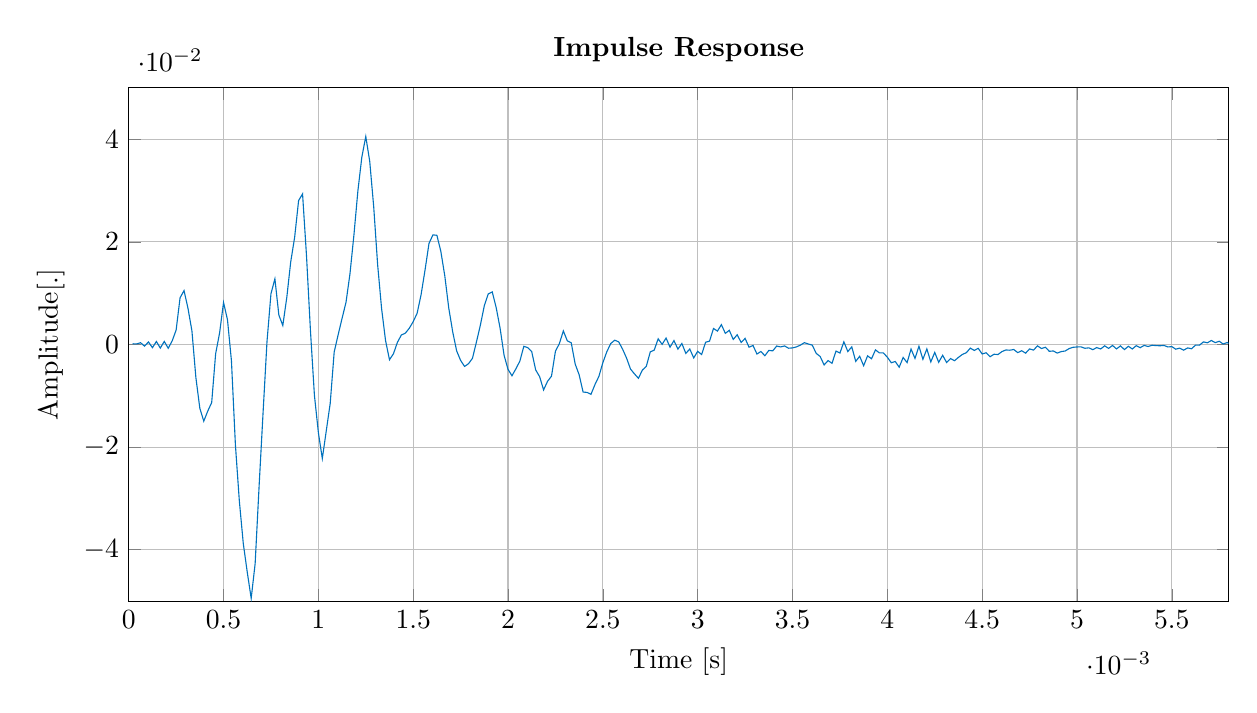
\begin{tikzpicture}

\begin{axis}[%
width=5.5in,
height=2.566in,
at={(0.758in,0.481in)},
scale only axis,
xmin=0,
xmax=0.0058,
xlabel={Time [s]},
xmajorgrids,
ymin=-0.05,
ymax=0.05,
ylabel={Amplitude[.]},
ymajorgrids,
axis background/.style={fill=white},
title style={font=\bfseries},
title={Impulse Response}
]
\addplot [color=mycolor1,solid,forget plot]
  table[row sep=crcr]{%
2.08333333333333e-05	0.000135433913215334\\
2.08333333333333e-05	0.000135433913215334\\
4.16666666666667e-05	0.00010428347781361\\
4.16666666666667e-05	0.00010428347781361\\
6.25e-05	0.000344413334139864\\
6.25e-05	0.000344413334139864\\
8.33333333333333e-05	-0.000326787629993873\\
8.33333333333333e-05	-0.000326787629993873\\
0.000104166666666667	0.000487962355576639\\
0.000104166666666667	0.000487962355576639\\
0.000125	-0.00062799062163618\\
0.000125	-0.00062799062163618\\
0.000145833333333333	0.000577837048121023\\
0.000145833333333333	0.000577837048121023\\
0.000166666666666667	-0.000705936720951288\\
0.000166666666666667	-0.000705936720951288\\
0.0001875	0.000596632997186765\\
0.0001875	0.000596632997186765\\
0.000208333333333333	-0.000744801783979219\\
0.000208333333333333	-0.000744801783979219\\
0.000229166666666667	0.000693026461965811\\
0.000229166666666667	0.000693026461965811\\
0.00025	0.00280096178642279\\
0.00025	0.00280096178642279\\
0.000270833333333333	0.00910447245025194\\
0.000270833333333333	0.00910447245025194\\
0.000291666666666667	0.010497050126642\\
0.000291666666666667	0.010497050126642\\
0.0003125	0.00704760015326353\\
0.0003125	0.00704760015326353\\
0.000333333333333333	0.00264053604855475\\
0.000333333333333333	0.00264053604855475\\
0.000354166666666667	-0.00644761957942986\\
0.000354166666666667	-0.00644761957942986\\
0.000375	-0.0124338902712034\\
0.000375	-0.0124338902712034\\
0.000395833333333333	-0.014944102564301\\
0.000395833333333333	-0.014944102564301\\
0.000416666666666667	-0.0129889330975951\\
0.000416666666666667	-0.0129889330975951\\
0.0004375	-0.0113228012066889\\
0.0004375	-0.0113228012066889\\
0.000458333333333333	-0.0018083924025413\\
0.000458333333333333	-0.0018083924025413\\
0.000479166666666667	0.00223685595257359\\
0.000479166666666667	0.00223685595257359\\
0.0005	0.00818035990653494\\
0.0005	0.00818035990653494\\
0.000520833333333333	0.00481451461250904\\
0.000520833333333333	0.00481451461250904\\
0.000541666666666667	-0.00318070505197419\\
0.000541666666666667	-0.00318070505197419\\
0.0005625	-0.0195147331246666\\
0.0005625	-0.0195147331246666\\
0.000583333333333333	-0.0305061541974751\\
0.000583333333333333	-0.0305061541974751\\
0.000604166666666667	-0.0388069079363328\\
0.000604166666666667	-0.0388069079363328\\
0.000625	-0.0443597787392153\\
0.000625	-0.0443597787392153\\
0.000645833333333333	-0.04947248649344\\
0.000645833333333333	-0.04947248649344\\
0.000666666666666667	-0.0426889454714648\\
0.000666666666666667	-0.0426889454714648\\
0.0006875	-0.027623454416695\\
0.0006875	-0.027623454416695\\
0.000708333333333333	-0.0133565686874192\\
0.000708333333333333	-0.0133565686874192\\
0.000729166666666667	0.000569393625168831\\
0.000729166666666667	0.000569393625168831\\
0.00075	0.009876606886302\\
0.00075	0.009876606886302\\
0.000770833333333333	0.0127893510967868\\
0.000770833333333333	0.0127893510967868\\
0.000791666666666667	0.00572944194755013\\
0.000791666666666667	0.00572944194755013\\
0.0008125	0.00369859578183801\\
0.0008125	0.00369859578183801\\
0.000833333333333333	0.00910966047294525\\
0.000833333333333333	0.00910966047294525\\
0.000854166666666667	0.0160692743719652\\
0.000854166666666667	0.0160692743719652\\
0.000875	0.0209095091706025\\
0.000875	0.0209095091706025\\
0.000895833333333333	0.0280558893246079\\
0.000895833333333333	0.0280558893246079\\
0.000916666666666667	0.0293281257378195\\
0.000916666666666667	0.0293281257378195\\
0.0009375	0.0172664823870042\\
0.0009375	0.0172664823870042\\
0.000958333333333333	0.0026421583954951\\
0.000958333333333333	0.0026421583954951\\
0.000979166666666667	-0.00988958569926237\\
0.000979166666666667	-0.00988958569926237\\
0.001	-0.0171570400100217\\
0.001	-0.0171570400100217\\
0.00102083333333333	-0.0222302951794128\\
0.00102083333333333	-0.0222302951794128\\
0.00104166666666667	-0.0168330692068472\\
0.00104166666666667	-0.0168330692068472\\
0.0010625	-0.0114628371058372\\
0.0010625	-0.0114628371058372\\
0.00108333333333333	-0.00148573608889458\\
0.00108333333333333	-0.00148573608889458\\
0.00110416666666667	0.0018725964322826\\
0.00110416666666667	0.0018725964322826\\
0.001125	0.00509272239150512\\
0.001125	0.00509272239150512\\
0.00114583333333333	0.00823233886452021\\
0.00114583333333333	0.00823233886452021\\
0.00116666666666667	0.0137789886038606\\
0.00116666666666667	0.0137789886038606\\
0.0011875	0.0213364980716123\\
0.0011875	0.0213364980716123\\
0.00120833333333333	0.0299066598605945\\
0.00120833333333333	0.0299066598605945\\
0.00122916666666667	0.0365029392969689\\
0.00122916666666667	0.0365029392969689\\
0.00125	0.0405221121651264\\
0.00125	0.0405221121651264\\
0.00127083333333333	0.0356842640516079\\
0.00127083333333333	0.0356842640516079\\
0.00129166666666667	0.026889505609109\\
0.00129166666666667	0.026889505609109\\
0.0013125	0.0155518471750642\\
0.0013125	0.0155518471750642\\
0.00133333333333333	0.00701436313374686\\
0.00133333333333333	0.00701436313374686\\
0.00135416666666667	0.000772712731335588\\
0.00135416666666667	0.000772712731335588\\
0.001375	-0.00298244286175644\\
0.001375	-0.00298244286175644\\
0.00139583333333333	-0.00181466811149981\\
0.00139583333333333	-0.00181466811149981\\
0.00141666666666667	0.000404369297381074\\
0.00141666666666667	0.000404369297381074\\
0.0014375	0.00183869657916399\\
0.0014375	0.00183869657916399\\
0.00145833333333333	0.00220238854363219\\
0.00145833333333333	0.00220238854363219\\
0.00147916666666667	0.0031466937397447\\
0.00147916666666667	0.0031466937397447\\
0.0015	0.00444756200564868\\
0.0015	0.00444756200564868\\
0.00152083333333333	0.00609519336366465\\
0.00152083333333333	0.00609519336366465\\
0.00154166666666667	0.0097164844299609\\
0.00154166666666667	0.0097164844299609\\
0.0015625	0.0145138769648296\\
0.0015625	0.0145138769648296\\
0.00158333333333333	0.0196950196395143\\
0.00158333333333333	0.0196950196395143\\
0.00160416666666667	0.0213610661039502\\
0.00160416666666667	0.0213610661039502\\
0.001625	0.0212700460484263\\
0.001625	0.0212700460484263\\
0.00164583333333333	0.0181253129023516\\
0.00164583333333333	0.0181253129023516\\
0.00166666666666667	0.0133550584290801\\
0.00166666666666667	0.0133550584290801\\
0.0016875	0.00709502508390666\\
0.0016875	0.00709502508390666\\
0.00170833333333333	0.00245043254398667\\
0.00170833333333333	0.00245043254398667\\
0.00172916666666667	-0.00125710768349322\\
0.00172916666666667	-0.00125710768349322\\
0.00175	-0.00310179376201682\\
0.00175	-0.00310179376201682\\
0.00177083333333333	-0.0042833471927695\\
0.00177083333333333	-0.0042833471927695\\
0.00179166666666667	-0.00375059392346641\\
0.00179166666666667	-0.00375059392346641\\
0.0018125	-0.00268920903022163\\
0.0018125	-0.00268920903022163\\
0.00183333333333333	0.000460889606385282\\
0.00183333333333333	0.000460889606385282\\
0.00185416666666667	0.00376130028158443\\
0.00185416666666667	0.00376130028158443\\
0.001875	0.00755722136328623\\
0.001875	0.00755722136328623\\
0.00189583333333333	0.00985496341934416\\
0.00189583333333333	0.00985496341934416\\
0.00191666666666667	0.0102471578137279\\
0.00191666666666667	0.0102471578137279\\
0.0019375	0.00719802860638345\\
0.0019375	0.00719802860638345\\
0.00195833333333333	0.00314215506598026\\
0.00195833333333333	0.00314215506598026\\
0.00197916666666667	-0.00210027495431218\\
0.00197916666666667	-0.00210027495431218\\
0.002	-0.0048509738070189\\
0.002	-0.0048509738070189\\
0.00202083333333333	-0.00609375993754162\\
0.00202083333333333	-0.00609375993754162\\
0.00204166666666667	-0.00474043824593231\\
0.00204166666666667	-0.00474043824593231\\
0.0020625	-0.00323003095864485\\
0.0020625	-0.00323003095864485\\
0.00208333333333333	-0.000360620347968937\\
0.00208333333333333	-0.000360620347968937\\
0.00210416666666667	-0.00061633142550342\\
0.00210416666666667	-0.00061633142550342\\
0.002125	-0.00140691942522913\\
0.002125	-0.00140691942522913\\
0.00214583333333333	-0.00496314204296772\\
0.00214583333333333	-0.00496314204296772\\
0.00216666666666667	-0.00627078009884212\\
0.00216666666666667	-0.00627078009884212\\
0.0021875	-0.00886126597765237\\
0.0021875	-0.00886126597765237\\
0.00220833333333333	-0.00718503426745825\\
0.00220833333333333	-0.00718503426745825\\
0.00222916666666667	-0.00617979955247214\\
0.00222916666666667	-0.00617979955247214\\
0.00225	-0.00132398039958444\\
0.00225	-0.00132398039958444\\
0.00227083333333333	0.000182596795236857\\
0.00227083333333333	0.000182596795236857\\
0.00229166666666667	0.0026345798079413\\
0.00229166666666667	0.0026345798079413\\
0.0023125	0.000721701257136711\\
0.0023125	0.000721701257136711\\
0.00233333333333333	0.00031469663168509\\
0.00233333333333333	0.00031469663168509\\
0.00235416666666667	-0.00381908545745833\\
0.00235416666666667	-0.00381908545745833\\
0.002375	-0.00591133646788777\\
0.002375	-0.00591133646788777\\
0.00239583333333333	-0.00926931648228275\\
0.00239583333333333	-0.00926931648228275\\
0.00241666666666667	-0.00934185888471153\\
0.00241666666666667	-0.00934185888471153\\
0.0024375	-0.00971184740565205\\
0.0024375	-0.00971184740565205\\
0.00245833333333333	-0.00781897163412688\\
0.00245833333333333	-0.00781897163412688\\
0.00247916666666667	-0.00621608190330788\\
0.00247916666666667	-0.00621608190330788\\
0.0025	-0.0035451727200707\\
0.0025	-0.0035451727200707\\
0.00252083333333333	-0.00142594728571806\\
0.00252083333333333	-0.00142594728571806\\
0.00254166666666667	0.000194955758886498\\
0.00254166666666667	0.000194955758886498\\
0.0025625	0.000827804421929125\\
0.0025625	0.000827804421929125\\
0.00258333333333333	0.000516094935541278\\
0.00258333333333333	0.000516094935541278\\
0.00260416666666667	-0.000918614368227631\\
0.00260416666666667	-0.000918614368227631\\
0.002625	-0.00265049428280117\\
0.002625	-0.00265049428280117\\
0.00264583333333333	-0.00478865678177032\\
0.00264583333333333	-0.00478865678177032\\
0.00266666666666667	-0.00572778906942212\\
0.00266666666666667	-0.00572778906942212\\
0.0026875	-0.006591813167025\\
0.0026875	-0.006591813167025\\
0.00270833333333333	-0.00500265460857434\\
0.00270833333333333	-0.00500265460857434\\
0.00272916666666667	-0.00424943177290689\\
0.00272916666666667	-0.00424943177290689\\
0.00275	-0.00145257330899368\\
0.00275	-0.00145257330899368\\
0.00277083333333333	-0.00109887914112521\\
0.00277083333333333	-0.00109887914112521\\
0.00279166666666667	0.00110193954463072\\
0.00279166666666667	0.00110193954463072\\
0.0028125	3.01018559236125e-05\\
0.0028125	3.01018559236125e-05\\
0.00283333333333333	0.00124412895192947\\
0.00283333333333333	0.00124412895192947\\
0.00285416666666667	-0.000526696911361515\\
0.00285416666666667	-0.000526696911361515\\
0.002875	0.000751907209861334\\
0.002875	0.000751907209861334\\
0.00289583333333333	-0.00090415267463952\\
0.00289583333333333	-0.00090415267463952\\
0.00291666666666667	0.000190371188907451\\
0.00291666666666667	0.000190371188907451\\
0.0029375	-0.00173943600592198\\
0.0029375	-0.00173943600592198\\
0.00295833333333333	-0.000884096434942723\\
0.00295833333333333	-0.000884096434942723\\
0.00297916666666667	-0.00262098030800951\\
0.00297916666666667	-0.00262098030800951\\
0.003	-0.00133668837589086\\
0.003	-0.00133668837589086\\
0.00302083333333333	-0.00195957524196219\\
0.00302083333333333	-0.00195957524196219\\
0.00304166666666667	0.000432804477009531\\
0.00304166666666667	0.000432804477009531\\
0.0030625	0.000646657157786062\\
0.0030625	0.000646657157786062\\
0.00308333333333333	0.0031130794573549\\
0.00308333333333333	0.0031130794573549\\
0.00310416666666667	0.00260967272278695\\
0.00310416666666667	0.00260967272278695\\
0.003125	0.00385967312825822\\
0.003125	0.00385967312825822\\
0.00314583333333333	0.00216725487377011\\
0.00314583333333333	0.00216725487377011\\
0.00316666666666667	0.0027541451382836\\
0.00316666666666667	0.0027541451382836\\
0.0031875	0.00098374171088158\\
0.0031875	0.00098374171088158\\
0.00320833333333333	0.00188703508986198\\
0.00320833333333333	0.00188703508986198\\
0.00322916666666667	0.000393221899759972\\
0.00322916666666667	0.000393221899759972\\
0.00325	0.00117865152148785\\
0.00325	0.00117865152148785\\
0.00327083333333333	-0.000531954290629303\\
0.00327083333333333	-0.000531954290629303\\
0.00329166666666667	-0.000189602478741491\\
0.00329166666666667	-0.000189602478741491\\
0.0033125	-0.00186363126658443\\
0.0033125	-0.00186363126658443\\
0.00333333333333333	-0.00136896921998027\\
0.00333333333333333	-0.00136896921998027\\
0.00335416666666667	-0.00219207881294614\\
0.00335416666666667	-0.00219207881294614\\
0.003375	-0.00116116027205154\\
0.003375	-0.00116116027205154\\
0.00339583333333333	-0.00123983942307146\\
0.00339583333333333	-0.00123983942307146\\
0.00341666666666667	-0.000304884150285724\\
0.00341666666666667	-0.000304884150285724\\
0.0034375	-0.000481949830763189\\
0.0034375	-0.000481949830763189\\
0.00345833333333333	-0.00029148602557637\\
0.00345833333333333	-0.00029148602557637\\
0.00347916666666667	-0.000729474392605956\\
0.00347916666666667	-0.000729474392605956\\
0.0035	-0.000672114193420604\\
0.0035	-0.000672114193420604\\
0.00352083333333333	-0.00046810148632148\\
0.00352083333333333	-0.00046810148632148\\
0.00354166666666667	-0.000127444626892088\\
0.00354166666666667	-0.000127444626892088\\
0.0035625	0.000347996161612028\\
0.0035625	0.000347996161612028\\
0.00358333333333333	8.84517752371697e-05\\
0.00358333333333333	8.84517752371697e-05\\
0.00360416666666667	-0.000122752956693136\\
0.00360416666666667	-0.000122752956693136\\
0.003625	-0.00173579753621118\\
0.003625	-0.00173579753621118\\
0.00364583333333333	-0.00234484697252995\\
0.00364583333333333	-0.00234484697252995\\
0.00366666666666667	-0.00398764315590221\\
0.00366666666666667	-0.00398764315590221\\
0.0036875	-0.0031423490024192\\
0.0036875	-0.0031423490024192\\
0.00370833333333333	-0.0036667740008205\\
0.00370833333333333	-0.0036667740008205\\
0.00372916666666667	-0.00128875782275372\\
0.00372916666666667	-0.00128875782275372\\
0.00375	-0.0016735392400399\\
0.00375	-0.0016735392400399\\
0.00377083333333333	0.000514780220675258\\
0.00377083333333333	0.000514780220675258\\
0.00379166666666667	-0.001379146732251\\
0.00379166666666667	-0.001379146732251\\
0.0038125	-0.000461484655572132\\
0.0038125	-0.000461484655572132\\
0.00383333333333333	-0.00328852194417925\\
0.00383333333333333	-0.00328852194417925\\
0.00385416666666667	-0.00229710003840595\\
0.00385416666666667	-0.00229710003840595\\
0.003875	-0.00413907992495678\\
0.003875	-0.00413907992495678\\
0.00389583333333333	-0.00221612572577929\\
0.00389583333333333	-0.00221612572577929\\
0.00391666666666667	-0.00278608071414276\\
0.00391666666666667	-0.00278608071414276\\
0.0039375	-0.00105407082810224\\
0.0039375	-0.00105407082810224\\
0.00395833333333333	-0.00165158409549926\\
0.00395833333333333	-0.00165158409549926\\
0.00397916666666667	-0.00165056187709485\\
0.00397916666666667	-0.00165056187709485\\
0.004	-0.00248280483288634\\
0.004	-0.00248280483288634\\
0.00402083333333333	-0.0035635693045157\\
0.00402083333333333	-0.0035635693045157\\
0.00404166666666667	-0.00332096993887084\\
0.00404166666666667	-0.00332096993887084\\
0.0040625	-0.00442700733465438\\
0.0040625	-0.00442700733465438\\
0.00408333333333333	-0.00253456677824636\\
0.00408333333333333	-0.00253456677824636\\
0.00410416666666667	-0.00353035634181479\\
0.00410416666666667	-0.00353035634181479\\
0.004125	-0.000889736199121273\\
0.004125	-0.000889736199121273\\
0.00414583333333333	-0.00271643930209907\\
0.00414583333333333	-0.00271643930209907\\
0.00416666666666667	-0.000348091605270431\\
0.00416666666666667	-0.000348091605270431\\
0.0041875	-0.00288474294884684\\
0.0041875	-0.00288474294884684\\
0.00420833333333333	-0.000872004431195904\\
0.00420833333333333	-0.000872004431195904\\
0.00422916666666667	-0.00339736640598935\\
0.00422916666666667	-0.00339736640598935\\
0.00425	-0.00154834523602723\\
0.00425	-0.00154834523602723\\
0.00427083333333333	-0.0034703032104403\\
0.00427083333333333	-0.0034703032104403\\
0.00429166666666667	-0.00210674687236268\\
0.00429166666666667	-0.00210674687236268\\
0.0043125	-0.00351559774510017\\
0.0043125	-0.00351559774510017\\
0.00433333333333333	-0.00273805789567693\\
0.00433333333333333	-0.00273805789567693\\
0.00435416666666667	-0.00316322848767519\\
0.00435416666666667	-0.00316322848767519\\
0.004375	-0.00251361301041933\\
0.004375	-0.00251361301041933\\
0.00439583333333333	-0.00194042978172852\\
0.00439583333333333	-0.00194042978172852\\
0.00441666666666667	-0.00159943477622404\\
0.00441666666666667	-0.00159943477622404\\
0.0044375	-0.000711365424097582\\
0.0044375	-0.000711365424097582\\
0.00445833333333333	-0.00116321288411866\\
0.00445833333333333	-0.00116321288411866\\
0.00447916666666667	-0.000753051899018485\\
0.00447916666666667	-0.000753051899018485\\
0.0045	-0.00185282248725731\\
0.0045	-0.00185282248725731\\
0.00452083333333333	-0.00161557409955166\\
0.00452083333333333	-0.00161557409955166\\
0.00454166666666667	-0.00238844327679989\\
0.00454166666666667	-0.00238844327679989\\
0.0045625	-0.00190398294782828\\
0.0045625	-0.00190398294782828\\
0.00458333333333333	-0.00196358474761833\\
0.00458333333333333	-0.00196358474761833\\
0.00460416666666667	-0.0013924025783961\\
0.00460416666666667	-0.0013924025783961\\
0.004625	-0.00106856056634697\\
0.004625	-0.00106856056634697\\
0.00464583333333333	-0.00111803494155153\\
0.00464583333333333	-0.00111803494155153\\
0.00466666666666667	-0.000980798466338009\\
0.00466666666666667	-0.000980798466338009\\
0.0046875	-0.00158607859441582\\
0.0046875	-0.00158607859441582\\
0.00470833333333333	-0.0012225690843977\\
0.00470833333333333	-0.0012225690843977\\
0.00472916666666667	-0.00169055261890915\\
0.00472916666666667	-0.00169055261890915\\
0.00475	-0.00086472642752262\\
0.00475	-0.00086472642752262\\
0.00477083333333333	-0.00110058019316083\\
0.00477083333333333	-0.00110058019316083\\
0.00479166666666667	-0.000263301192092161\\
0.00479166666666667	-0.000263301192092161\\
0.0048125	-0.000787826659008271\\
0.0048125	-0.000787826659008271\\
0.00483333333333333	-0.000545149553754871\\
0.00483333333333333	-0.000545149553754871\\
0.00485416666666667	-0.00133712497165648\\
0.00485416666666667	-0.00133712497165648\\
0.004875	-0.00125982170062951\\
0.004875	-0.00125982170062951\\
0.00489583333333333	-0.00167918214879971\\
0.00489583333333333	-0.00167918214879971\\
0.00491666666666667	-0.00138718157995743\\
0.00491666666666667	-0.00138718157995743\\
0.0049375	-0.00127540222099471\\
0.0049375	-0.00127540222099471\\
0.00495833333333333	-0.000806129133631623\\
0.00495833333333333	-0.000806129133631623\\
0.00497916666666667	-0.0005539060189666\\
0.00497916666666667	-0.0005539060189666\\
0.005	-0.000485068056610165\\
0.005	-0.000485068056610165\\
0.00502083333333333	-0.000466778724461535\\
0.00502083333333333	-0.000466778724461535\\
0.00504166666666667	-0.000744187472974092\\
0.00504166666666667	-0.000744187472974092\\
0.0050625	-0.000654976302911786\\
0.0050625	-0.000654976302911786\\
0.00508333333333333	-0.00101062169659435\\
0.00508333333333333	-0.00101062169659435\\
0.00510416666666667	-0.00060694991646005\\
0.00510416666666667	-0.00060694991646005\\
0.005125	-0.000877628766758219\\
0.005125	-0.000877628766758219\\
0.00514583333333333	-0.000265613658124843\\
0.00514583333333333	-0.000265613658124843\\
0.00516666666666667	-0.000764358658186385\\
0.00516666666666667	-0.000764358658186385\\
0.0051875	-0.000191100806120372\\
0.0051875	-0.000191100806120372\\
0.00520833333333333	-0.000867845302083077\\
0.00520833333333333	-0.000867845302083077\\
0.00522916666666667	-0.000275576980375711\\
0.00522916666666667	-0.000275576980375711\\
0.00525	-0.000994566502820595\\
0.00525	-0.000994566502820595\\
0.00527083333333333	-0.000352381999584851\\
0.00527083333333333	-0.000352381999584851\\
0.00529166666666667	-0.000882347765159384\\
0.00529166666666667	-0.000882347765159384\\
0.0053125	-0.000226685868454497\\
0.0053125	-0.000226685868454497\\
0.00533333333333333	-0.000626690991383088\\
0.00533333333333333	-0.000626690991383088\\
0.00535416666666667	-0.000177632693546326\\
0.00535416666666667	-0.000177632693546326\\
0.005375	-0.000398853369473559\\
0.005375	-0.000398853369473559\\
0.00539583333333333	-0.000154193313898835\\
0.00539583333333333	-0.000154193313898835\\
0.00541666666666667	-0.000218177875922818\\
0.00541666666666667	-0.000218177875922818\\
0.0054375	-0.000253007969614311\\
0.0054375	-0.000253007969614311\\
0.00545833333333333	-0.000183919964304681\\
0.00545833333333333	-0.000183919964304681\\
0.00547916666666667	-0.000482695162058063\\
0.00547916666666667	-0.000482695162058063\\
0.0055	-0.000417122283707766\\
0.0055	-0.000417122283707766\\
0.00552083333333333	-0.000918754285558994\\
0.00552083333333333	-0.000918754285558994\\
0.00554166666666667	-0.00070926587719205\\
0.00554166666666667	-0.00070926587719205\\
0.0055625	-0.00111176108389037\\
0.0055625	-0.00111176108389037\\
0.00558333333333333	-0.000671692641021206\\
0.00558333333333333	-0.000671692641021206\\
0.00560416666666667	-0.000832207440490903\\
0.00560416666666667	-0.000832207440490903\\
0.005625	-0.000121396509376363\\
0.005625	-0.000121396509376363\\
0.00564583333333333	-0.000141313736190993\\
0.00564583333333333	-0.000141313736190993\\
0.00566666666666667	0.000505737924435369\\
0.00566666666666667	0.000505737924435369\\
0.0056875	0.000325280340334074\\
0.0056875	0.000325280340334074\\
0.00570833333333333	0.000775749985311516\\
0.00570833333333333	0.000775749985311516\\
0.00572916666666667	0.000356869910858819\\
0.00572916666666667	0.000356869910858819\\
0.00575	0.00062719857031549\\
0.00575	0.00062719857031549\\
0.00577083333333333	8.4113034534751e-05\\
0.00577083333333333	8.4113034534751e-05\\
0.00579166666666667	0.00038108121252198\\
0.00579166666666667	0.00038108121252198\\
0.0058125	-0.000121848016070046\\
0.0058125	-0.000121848016070046\\
0.0058125	-0.000121848016070046\\
0.0058125	-0.000121848016070046\\
0.0058125	-0.000121848016070046\\
0.0058125	-0.000121848016070046\\
0.0058125	-0.000121848016070046\\
0.0058125	-0.000121848016070046\\
0.0058125	-0.000121848016070046\\
0.0058125	-0.000121848016070046\\
0.0058125	-0.000121848016070046\\
0.0058125	-0.000121848016070046\\
0.0058125	-0.000121848016070046\\
0.0058125	-0.000121848016070046\\
0.0058125	-0.000121848016070046\\
0.0058125	-0.000121848016070046\\
0.0058125	-0.000121848016070046\\
0.0058125	-0.000121848016070046\\
0.0058125	-0.000121848016070046\\
0.0058125	-0.000121848016070046\\
0.0058125	-0.000121848016070046\\
0.0058125	-0.000121848016070046\\
0.0058125	-0.000121848016070046\\
0.0058125	-0.000121848016070046\\
0.0058125	-0.000121848016070046\\
0.0058125	-0.000121848016070046\\
0.0058125	-0.000121848016070046\\
0.0058125	-0.000121848016070046\\
0.0058125	-0.000121848016070046\\
0.0058125	-0.000121848016070046\\
0.0058125	-0.000121848016070046\\
0.0058125	-0.000121848016070046\\
0.0058125	-0.000121848016070046\\
0.0058125	-0.000121848016070046\\
0.0058125	-0.000121848016070046\\
0.0058125	-0.000121848016070046\\
0.0058125	-0.000121848016070046\\
0.0058125	-0.000121848016070046\\
0.0058125	-0.000121848016070046\\
0.0058125	-0.000121848016070046\\
0.0058125	-0.000121848016070046\\
0.0058125	-0.000121848016070046\\
0.0058125	-0.000121848016070046\\
0.0058125	-0.000121848016070046\\
0.0058125	-0.000121848016070046\\
0.0058125	-0.000121848016070046\\
0.0058125	-0.000121848016070046\\
0.0058125	-0.000121848016070046\\
0.0058125	-0.000121848016070046\\
0.0058125	-0.000121848016070046\\
0.0058125	-0.000121848016070046\\
0.0058125	-0.000121848016070046\\
0.0058125	-0.000121848016070046\\
0.0058125	-0.000121848016070046\\
0.0058125	-0.000121848016070046\\
0.0058125	-0.000121848016070046\\
0.0058125	-0.000121848016070046\\
0.0058125	-0.000121848016070046\\
0.0058125	-0.000121848016070046\\
0.0058125	-0.000121848016070046\\
0.0058125	-0.000121848016070046\\
0.0058125	-0.000121848016070046\\
0.0058125	-0.000121848016070046\\
0.0058125	-0.000121848016070046\\
0.0058125	-0.000121848016070046\\
0.0058125	-0.000121848016070046\\
0.0058125	-0.000121848016070046\\
0.0058125	-0.000121848016070046\\
0.0058125	-0.000121848016070046\\
0.0058125	-0.000121848016070046\\
0.0058125	-0.000121848016070046\\
0.0058125	-0.000121848016070046\\
0.0058125	-0.000121848016070046\\
0.0058125	-0.000121848016070046\\
0.0058125	-0.000121848016070046\\
0.0058125	-0.000121848016070046\\
0.0058125	-0.000121848016070046\\
0.0058125	-0.000121848016070046\\
0.0058125	-0.000121848016070046\\
0.0058125	-0.000121848016070046\\
0.0058125	-0.000121848016070046\\
0.0058125	-0.000121848016070046\\
0.0058125	-0.000121848016070046\\
0.0058125	-0.000121848016070046\\
0.0058125	-0.000121848016070046\\
0.0058125	-0.000121848016070046\\
0.0058125	-0.000121848016070046\\
0.0058125	-0.000121848016070046\\
0.0058125	-0.000121848016070046\\
0.0058125	-0.000121848016070046\\
0.0058125	-0.000121848016070046\\
0.0058125	-0.000121848016070046\\
0.0058125	-0.000121848016070046\\
0.0058125	-0.000121848016070046\\
0.0058125	-0.000121848016070046\\
0.0058125	-0.000121848016070046\\
0.0058125	-0.000121848016070046\\
0.0058125	-0.000121848016070046\\
0.0058125	-0.000121848016070046\\
0.0058125	-0.000121848016070046\\
0.0058125	-0.000121848016070046\\
0.0058125	-0.000121848016070046\\
0.0058125	-0.000121848016070046\\
0.0058125	-0.000121848016070046\\
0.0058125	-0.000121848016070046\\
0.0058125	-0.000121848016070046\\
0.0058125	-0.000121848016070046\\
0.0058125	-0.000121848016070046\\
0.0058125	-0.000121848016070046\\
0.0058125	-0.000121848016070046\\
0.0058125	-0.000121848016070046\\
0.0058125	-0.000121848016070046\\
0.0058125	-0.000121848016070046\\
0.0058125	-0.000121848016070046\\
0.0058125	-0.000121848016070046\\
0.0058125	-0.000121848016070046\\
0.0058125	-0.000121848016070046\\
0.0058125	-0.000121848016070046\\
0.0058125	-0.000121848016070046\\
0.0058125	-0.000121848016070046\\
0.0058125	-0.000121848016070046\\
0.0058125	-0.000121848016070046\\
0.0058125	-0.000121848016070046\\
0.0058125	-0.000121848016070046\\
0.0058125	-0.000121848016070046\\
0.0058125	-0.000121848016070046\\
0.0058125	-0.000121848016070046\\
0.0058125	-0.000121848016070046\\
0.0058125	-0.000121848016070046\\
0.0058125	-0.000121848016070046\\
0.0058125	-0.000121848016070046\\
0.0058125	-0.000121848016070046\\
0.0058125	-0.000121848016070046\\
0.0058125	-0.000121848016070046\\
0.0058125	-0.000121848016070046\\
0.0058125	-0.000121848016070046\\
0.0058125	-0.000121848016070046\\
0.0058125	-0.000121848016070046\\
0.0058125	-0.000121848016070046\\
0.0058125	-0.000121848016070046\\
0.0058125	-0.000121848016070046\\
0.0058125	-0.000121848016070046\\
0.0058125	-0.000121848016070046\\
0.0058125	-0.000121848016070046\\
0.0058125	-0.000121848016070046\\
0.0058125	-0.000121848016070046\\
0.0058125	-0.000121848016070046\\
0.0058125	-0.000121848016070046\\
0.0058125	-0.000121848016070046\\
0.0058125	-0.000121848016070046\\
0.0058125	-0.000121848016070046\\
0.0058125	-0.000121848016070046\\
0.0058125	-0.000121848016070046\\
0.0058125	-0.000121848016070046\\
0.0058125	-0.000121848016070046\\
0.0058125	-0.000121848016070046\\
0.0058125	-0.000121848016070046\\
0.0058125	-0.000121848016070046\\
0.0058125	-0.000121848016070046\\
0.0058125	-0.000121848016070046\\
0.0058125	-0.000121848016070046\\
0.0058125	-0.000121848016070046\\
0.0058125	-0.000121848016070046\\
0.0058125	-0.000121848016070046\\
0.0058125	-0.000121848016070046\\
0.0058125	-0.000121848016070046\\
0.0058125	-0.000121848016070046\\
0.0058125	-0.000121848016070046\\
0.0058125	-0.000121848016070046\\
0.0058125	-0.000121848016070046\\
0.0058125	-0.000121848016070046\\
0.0058125	-0.000121848016070046\\
0.0058125	-0.000121848016070046\\
0.0058125	-0.000121848016070046\\
0.0058125	-0.000121848016070046\\
0.0058125	-0.000121848016070046\\
0.0058125	-0.000121848016070046\\
0.0058125	-0.000121848016070046\\
0.0058125	-0.000121848016070046\\
0.0058125	-0.000121848016070046\\
0.0058125	-0.000121848016070046\\
0.0058125	-0.000121848016070046\\
0.0058125	-0.000121848016070046\\
0.0058125	-0.000121848016070046\\
0.0058125	-0.000121848016070046\\
0.0058125	-0.000121848016070046\\
0.0058125	-0.000121848016070046\\
0.0058125	-0.000121848016070046\\
0.0058125	-0.000121848016070046\\
0.0058125	-0.000121848016070046\\
0.0058125	-0.000121848016070046\\
0.0058125	-0.000121848016070046\\
0.0058125	-0.000121848016070046\\
0.0058125	-0.000121848016070046\\
0.0058125	-0.000121848016070046\\
0.0058125	-0.000121848016070046\\
0.0058125	-0.000121848016070046\\
0.0058125	-0.000121848016070046\\
0.0058125	-0.000121848016070046\\
0.0058125	-0.000121848016070046\\
0.0058125	-0.000121848016070046\\
0.0058125	-0.000121848016070046\\
0.0058125	-0.000121848016070046\\
0.0058125	-0.000121848016070046\\
0.0058125	-0.000121848016070046\\
0.0058125	-0.000121848016070046\\
0.0058125	-0.000121848016070046\\
0.0058125	-0.000121848016070046\\
0.0058125	-0.000121848016070046\\
0.0058125	-0.000121848016070046\\
0.0058125	-0.000121848016070046\\
0.0058125	-0.000121848016070046\\
0.0058125	-0.000121848016070046\\
0.0058125	-0.000121848016070046\\
0.0058125	-0.000121848016070046\\
0.0058125	-0.000121848016070046\\
0.0058125	-0.000121848016070046\\
0.0058125	-0.000121848016070046\\
0.0058125	-0.000121848016070046\\
0.0058125	-0.000121848016070046\\
0.0058125	-0.000121848016070046\\
0.0058125	-0.000121848016070046\\
0.0058125	-0.000121848016070046\\
0.0058125	-0.000121848016070046\\
0.0058125	-0.000121848016070046\\
0.0058125	-0.000121848016070046\\
0.0058125	-0.000121848016070046\\
0.0058125	-0.000121848016070046\\
0.0058125	-0.000121848016070046\\
0.0058125	-0.000121848016070046\\
0.0058125	-0.000121848016070046\\
0.0058125	-0.000121848016070046\\
0.0058125	-0.000121848016070046\\
0.0058125	-0.000121848016070046\\
0.0058125	-0.000121848016070046\\
0.0058125	-0.000121848016070046\\
0.0058125	-0.000121848016070046\\
0.0058125	-0.000121848016070046\\
0.0058125	-0.000121848016070046\\
0.0058125	-0.000121848016070046\\
0.0058125	-0.000121848016070046\\
0.0058125	-0.000121848016070046\\
0.0058125	-0.000121848016070046\\
0.0058125	-0.000121848016070046\\
0.0058125	-0.000121848016070046\\
0.0058125	-0.000121848016070046\\
0.0058125	-0.000121848016070046\\
0.0058125	-0.000121848016070046\\
0.0058125	-0.000121848016070046\\
0.0058125	-0.000121848016070046\\
0.0058125	-0.000121848016070046\\
0.0058125	-0.000121848016070046\\
0.0058125	-0.000121848016070046\\
0.0058125	-0.000121848016070046\\
0.0058125	-0.000121848016070046\\
0.0058125	-0.000121848016070046\\
0.0058125	-0.000121848016070046\\
0.0058125	-0.000121848016070046\\
0.0058125	-0.000121848016070046\\
0.0058125	-0.000121848016070046\\
0.0058125	-0.000121848016070046\\
0.0058125	-0.000121848016070046\\
0.0058125	-0.000121848016070046\\
0.0058125	-0.000121848016070046\\
0.0058125	-0.000121848016070046\\
0.0058125	-0.000121848016070046\\
0.0058125	-0.000121848016070046\\
0.0058125	-0.000121848016070046\\
0.0058125	-0.000121848016070046\\
0.0058125	-0.000121848016070046\\
0.0058125	-0.000121848016070046\\
0.0058125	-0.000121848016070046\\
0.0058125	-0.000121848016070046\\
0.0058125	-0.000121848016070046\\
0.0058125	-0.000121848016070046\\
0.0058125	-0.000121848016070046\\
0.0058125	-0.000121848016070046\\
0.0058125	-0.000121848016070046\\
0.0058125	-0.000121848016070046\\
0.0058125	-0.000121848016070046\\
0.0058125	-0.000121848016070046\\
0.0058125	-0.000121848016070046\\
0.0058125	-0.000121848016070046\\
0.0058125	-0.000121848016070046\\
0.0058125	-0.000121848016070046\\
0.0058125	-0.000121848016070046\\
0.0058125	-0.000121848016070046\\
0.0058125	-0.000121848016070046\\
0.0058125	-0.000121848016070046\\
0.0058125	-0.000121848016070046\\
0.0058125	-0.000121848016070046\\
0.0058125	-0.000121848016070046\\
0.0058125	-0.000121848016070046\\
0.0058125	-0.000121848016070046\\
0.0058125	-0.000121848016070046\\
0.0058125	-0.000121848016070046\\
0.0058125	-0.000121848016070046\\
0.0058125	-0.000121848016070046\\
0.0058125	-0.000121848016070046\\
0.0058125	-0.000121848016070046\\
0.0058125	-0.000121848016070046\\
0.0058125	-0.000121848016070046\\
0.0058125	-0.000121848016070046\\
0.0058125	-0.000121848016070046\\
0.0058125	-0.000121848016070046\\
0.0058125	-0.000121848016070046\\
0.0058125	-0.000121848016070046\\
0.0058125	-0.000121848016070046\\
0.0058125	-0.000121848016070046\\
0.0058125	-0.000121848016070046\\
0.0058125	-0.000121848016070046\\
0.0058125	-0.000121848016070046\\
};
\end{axis}
\end{tikzpicture}%
	\caption{Impulse Response plot of the headphones }
	\label{HeadPhoneImpulseResponse}
\end{figure}

%\begin{figure}[H]
%	\centering
%	\tikzsetnextfilename{CancellationPathImpulseResponse}
%	% This file was created by matlab2tikz.
%
%The latest updates can be retrieved from
%  http://www.mathworks.com/matlabcentral/fileexchange/22022-matlab2tikz-matlab2tikz
%where you can also make suggestions and rate matlab2tikz.
%
\definecolor{mycolor1}{rgb}{0.00000,0.44700,0.74100}%
\definecolor{mycolor2}{rgb}{0.85000,0.32500,0.09800}%
\definecolor{mycolor3}{rgb}{0.92900,0.69400,0.12500}%
\definecolor{mycolor4}{rgb}{0.49400,0.18400,0.55600}%
\definecolor{mycolor5}{rgb}{0.46600,0.67400,0.18800}%
%
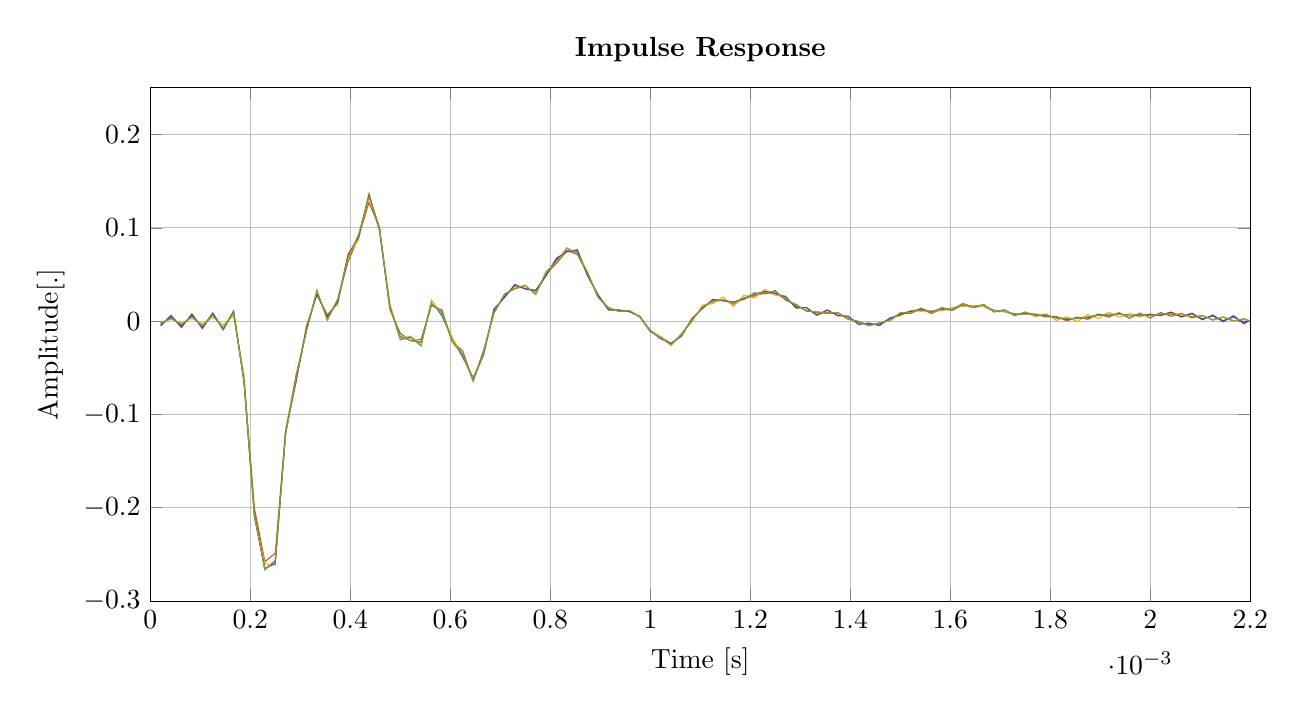
\begin{tikzpicture}

\begin{axis}[%
width=5.5in,
height=2.566in,
at={(0.758in,0.481in)},
scale only axis,
xmin=0,
xmax=0.0022,
xlabel={Time [s]},
xmajorgrids,
ymin=-0.30,
ymax=0.25,
ylabel={Amplitude[.]},
ymajorgrids,
axis background/.style={fill=white},
title style={font=\bfseries},
title={Impulse Response}
]
\addplot [color=mycolor1,solid,forget plot]
  table[row sep=crcr]{%
2.08333333333333e-05	-0.0037087927908794\\
4.16666666666667e-05	0.00421160453226942\\
6.25e-05	-0.00520379576953817\\
8.33333333333333e-05	0.00629701654848276\\
0.000104166666666667	-0.00678651279752952\\
0.000125	0.00811356819824401\\
0.000145833333333333	-0.00884124098433367\\
0.000166666666666667	0.0107472615560426\\
0.0001875	-0.0646663577808535\\
0.000208333333333333	-0.206299821990036\\
0.000229166666666667	-0.266170671528939\\
0.00025	-0.256370669612707\\
0.000270833333333333	-0.120287541326005\\
0.000291666666666667	-0.0617180208660174\\
0.0003125	-0.00922362905565283\\
0.000333333333333333	0.0308397018576189\\
0.000354166666666667	0.0035403786890247\\
0.000375	0.0212448332280645\\
0.000395833333333333	0.0705478621795121\\
0.000416666666666667	0.0895474948933934\\
0.0004375	0.13552149422923\\
0.000458333333333333	0.097299803954558\\
0.000479166666666667	0.0171466790731723\\
0.0005	-0.0197680684506663\\
0.000520833333333333	-0.0171223102171715\\
0.000541666666666667	-0.0263656309604829\\
0.0005625	0.0219768694253305\\
0.000583333333333333	0.00560475366613178\\
0.000604166666666667	-0.0182339778631218\\
0.000625	-0.0387957025837346\\
0.000645833333333333	-0.0604621915450745\\
0.000666666666666667	-0.0363795655357155\\
0.0006875	0.0130977677372803\\
0.000708333333333333	0.0251346467322033\\
0.000729166666666667	0.039105419651278\\
0.00075	0.0346523806957789\\
0.000770833333333333	0.0322481248629661\\
0.000791666666666667	0.0493725854189164\\
0.0008125	0.0660612053755624\\
0.000833333333333333	0.0751202061643853\\
0.000854166666666667	0.0750428627194294\\
0.000875	0.048916982972921\\
0.000895833333333333	0.0274042750529549\\
0.000916666666666667	0.012118310680073\\
0.0009375	0.0119101424242984\\
0.000958333333333333	0.0100853086322103\\
0.000979166666666667	0.00544456035302204\\
0.001	-0.0112918644454638\\
0.00102083333333333	-0.0172483398553776\\
0.00104166666666667	-0.0251189065330511\\
0.0010625	-0.014558012452602\\
0.00108333333333333	0.0017134948101292\\
0.00110416666666667	0.014255079903006\\
0.001125	0.0227537754361355\\
0.00114583333333333	0.021816701937651\\
0.00116666666666667	0.0206421122092443\\
0.0011875	0.0233880957023547\\
0.00120833333333333	0.0302390075091007\\
0.00122916666666667	0.0293537948171238\\
0.00125	0.0326242279536413\\
0.00127083333333333	0.0225148202302848\\
0.00129166666666667	0.0177894930311056\\
0.0013125	0.010770331824266\\
0.00133333333333333	0.00983620954713187\\
0.00135416666666667	0.00853521175516866\\
0.001375	0.00899597167105174\\
0.00139583333333333	0.00260243594654619\\
0.00141666666666667	-0.00104701561770118\\
0.0014375	-0.00371807000382697\\
0.00145833333333333	-0.00318960626194621\\
0.00147916666666667	0.00257545774845068\\
0.0015	0.00713790465040768\\
0.00152083333333333	0.0108215910141207\\
0.00154166666666667	0.0120264444758566\\
0.0015625	0.0108261870538285\\
0.00158333333333333	0.0123450686244096\\
0.00160416666666667	0.0139129670171921\\
0.001625	0.0169005010166529\\
0.00164583333333333	0.0165791257894914\\
0.00166666666666667	0.0159045477126551\\
0.0016875	0.0116907728854056\\
0.00170833333333333	0.0102974368732395\\
0.00172916666666667	0.00768755665771632\\
0.00175	0.0082004670345183\\
0.00177083333333333	0.00731505527542035\\
0.00179166666666667	0.0054086354181059\\
0.0018125	0.00446490364319473\\
0.00183333333333333	0.00151912598295708\\
0.00185416666666667	0.00374848548552877\\
0.001875	0.00361835820665017\\
0.00189583333333333	0.00680282624355538\\
0.00191666666666667	0.00648760855183481\\
0.0019375	0.00770072765347351\\
0.00195833333333333	0.00591670768911894\\
0.00197916666666667	0.00654249543276334\\
0.002	0.00696958712555653\\
0.00202083333333333	0.00639676696262537\\
0.00204166666666667	0.00930875870313683\\
0.0020625	0.00487368778960512\\
0.00208333333333333	0.00793267565500179\\
0.00210416666666667	0.00227381220914028\\
0.002125	0.00559059790855196\\
0.00214583333333333	0.000509710927088874\\
0.00216666666666667	0.00445914830547992\\
0.0021875	-0.0013119827312339\\
0.00220833333333333	0.00204620626659837\\
0.00222916666666667	-0.00226693806170011\\
0.00225	-0.000865052032163367\\
0.00227083333333333	-0.000568466635637404\\
0.00229166666666667	-0.00176072172101629\\
0.0023125	0.001051321525168\\
0.00233333333333333	-0.00235307840318451\\
0.00235416666666667	0.00142050267868398\\
0.002375	-0.00373732644882233\\
0.00239583333333333	0.00263329200115178\\
0.00241666666666667	-0.00419384885137344\\
0.0024375	0.00356243119561722\\
0.00245833333333333	-0.00341750395084726\\
0.00247916666666667	0.00231533516568704\\
0.0025	-0.002886346397735\\
0.00252083333333333	0.000637791268280785\\
0.00254166666666667	-0.00290884766679218\\
0.0025625	-0.000629280559252555\\
0.00258333333333333	-0.00286116806569122\\
0.00260416666666667	-0.00278592644964782\\
0.002625	-0.00262193859169995\\
0.00264583333333333	-0.00474810164470427\\
0.00266666666666667	-0.00275009938116807\\
0.0026875	-0.00478816826817122\\
0.00270833333333333	-0.00324811681170597\\
0.00272916666666667	-0.0040257377623872\\
0.00275	-0.00368074892796126\\
0.00277083333333333	-0.00337062684290595\\
0.00279166666666667	-0.00370307569447635\\
0.0028125	-0.00186571326957182\\
0.00283333333333333	-0.00390602380821677\\
0.00285416666666667	-4.9752550230383e-05\\
0.002875	-0.00438323194808954\\
0.00289583333333333	0.000384386269952189\\
0.00291666666666667	-0.00453307061294354\\
0.0029375	-0.000328341601327697\\
0.00295833333333333	-0.00426336185525099\\
0.00297916666666667	-0.00128138687597425\\
0.003	-0.00414308057749922\\
0.00302083333333333	-0.00248651642821263\\
0.00304166666666667	-0.00361961427656752\\
0.0030625	-0.00400763468176544\\
0.00308333333333333	-0.0023795304299123\\
0.00310416666666667	-0.00514325156697817\\
0.003125	-0.00122625577194359\\
0.00314583333333333	-0.00545188790289689\\
0.00316666666666667	-0.000609928041986866\\
0.0031875	-0.00505013848995181\\
0.00320833333333333	5.99816839252916e-05\\
0.00322916666666667	-0.00449193406111753\\
0.00325	0.000558016389499313\\
0.00327083333333333	-0.00386841737730755\\
0.00329166666666667	0.000169965391614449\\
0.0033125	-0.00319883141842068\\
0.00333333333333333	-0.000671676767081501\\
0.00335416666666667	-0.00289606776507812\\
0.003375	-0.00113994195612087\\
0.00339583333333333	-0.00325262465554565\\
0.00341666666666667	-0.00136179764715377\\
0.0034375	-0.00360873416552366\\
0.00345833333333333	-0.00164463882761736\\
0.00347916666666667	-0.00371793269729748\\
0.0035	-0.00154353439141849\\
0.00352083333333333	-0.00403549855695194\\
0.00354166666666667	-0.000984353596708564\\
0.0035625	-0.00425443771279568\\
0.00358333333333333	-0.000672628985252431\\
0.00360416666666667	-0.00374129885739169\\
0.003625	-0.000937340861272143\\
0.00364583333333333	-0.00296533591369333\\
0.00366666666666667	-0.00130448571666488\\
0.0036875	-0.00246387735925147\\
0.00370833333333333	-0.00182327238315157\\
0.00372916666666667	-0.00173617907905828\\
0.00375	-0.00284258077794951\\
0.00377083333333333	-0.000756536202756666\\
0.00379166666666667	-0.00385114062696801\\
0.0038125	-0.000291952662999003\\
0.00383333333333333	-0.00423039940178691\\
0.00385416666666667	-0.000378549414924021\\
0.003875	-0.00428312305197425\\
0.00389583333333333	-0.000406743035733924\\
0.00391666666666667	-0.00424392197549792\\
0.0039375	-0.000625284040186809\\
0.00395833333333333	-0.00365167293604246\\
0.00397916666666667	-0.001337671135446\\
0.004	-0.00271896198950253\\
0.00402083333333333	-0.0019858020567554\\
0.00404166666666667	-0.00219062801883803\\
0.0040625	-0.00220835913204532\\
0.00408333333333333	-0.00203974929682549\\
0.00410416666666667	-0.00233913427988745\\
0.004125	-0.00185099449592134\\
0.00414583333333333	-0.00236574968059208\\
0.00416666666666667	-0.00196457798952639\\
0.0041875	-0.0019046742644009\\
0.00420833333333333	-0.00250443960036927\\
0.00422916666666667	-0.00128461530764495\\
0.00425	-0.00297296735967611\\
0.00427083333333333	-0.000992836466506577\\
0.00429166666666667	-0.00314961192994209\\
0.0043125	-0.000907894618487529\\
0.00433333333333333	-0.00328775019087989\\
0.00435416666666667	-0.000812410858858454\\
0.004375	-0.00329843852206017\\
0.00439583333333333	-0.000993520893343976\\
0.00441666666666667	-0.00296787895096846\\
0.0044375	-0.00135986816935005\\
0.00445833333333333	-0.00257683158276436\\
0.00447916666666667	-0.00150120312434058\\
0.0045	-0.00246875060820952\\
0.00452083333333333	-0.00127751762473565\\
0.00454166666666667	-0.00257055972440008\\
0.0045625	-0.000850583087086702\\
0.00458333333333333	-0.00279615291783079\\
0.00460416666666667	-0.000169229703961833\\
0.004625	-0.0033208199374696\\
0.00464583333333333	0.000762775063455069\\
0.00466666666666667	-0.00404729208587363\\
0.0046875	0.00162126259324774\\
0.00470833333333333	-0.00461429328418873\\
0.00472916666666667	0.00206634843487202\\
0.00475	-0.00479804415433337\\
0.00477083333333333	0.00203716599298341\\
0.00479166666666667	-0.00461953370883597\\
0.0048125	0.00158614710765907\\
0.00483333333333333	-0.0039600168009732\\
0.00485416666666667	0.00066992915889739\\
0.004875	-0.0027700643584047\\
0.00489583333333333	-0.000614917555245659\\
0.00491666666666667	-0.00132297677247495\\
0.0049375	-0.00190838752526078\\
0.00495833333333333	-4.06116797333875e-05\\
0.00497916666666667	-0.00288565901097666\\
0.005	0.000889847654868419\\
0.00502083333333333	-0.00349274225205263\\
0.00504166666666667	0.00137995835933047\\
0.0050625	-0.00358103532986242\\
0.00508333333333333	0.00125952593606002\\
0.00510416666666667	-0.00298112408616989\\
0.005125	0.00052817856633219\\
0.00514583333333333	-0.0019103540353447\\
0.00516666666666667	-0.000471366982676235\\
0.0051875	-0.000794234842926538\\
0.00520833333333333	-0.00141585678773726\\
};
\addplot [color=mycolor2,solid,forget plot]
  table[row sep=crcr]{%
2.08333333333333e-05	-0.00255267252938673\\
4.16666666666667e-05	0.00289958707347902\\
6.25e-05	-0.00382265239043665\\
8.33333333333333e-05	0.00482200108963299\\
0.000104166666666667	-0.00515633007307537\\
0.000125	0.00667606380308441\\
0.000145833333333333	-0.00708343055179381\\
0.000166666666666667	0.0092525375696961\\
0.0001875	-0.0607390597290135\\
0.000208333333333333	-0.200401659875795\\
0.000229166666666667	-0.257768300997275\\
0.00025	-0.248800582164502\\
0.000270833333333333	-0.117646720461853\\
0.000291666666666667	-0.0578844981508881\\
0.0003125	-0.0102016454149929\\
0.000333333333333333	0.0330014197433572\\
0.000354166666666667	0.00127667958148536\\
0.000375	0.0234190373569384\\
0.000395833333333333	0.0639275956854277\\
0.000416666666666667	0.0906470163865055\\
0.0004375	0.127123824348622\\
0.000458333333333333	0.100636329904299\\
0.000479166666666667	0.0124905457764127\\
0.0005	-0.0128509224250364\\
0.000520833333333333	-0.0212238017533485\\
0.000541666666666667	-0.0195717514784339\\
0.0005625	0.0166431551373302\\
0.000583333333333333	0.0120320299572739\\
0.000604166666666667	-0.0219158802601074\\
0.000625	-0.0320151869444835\\
0.000645833333333333	-0.0633380264022395\\
0.000666666666666667	-0.0314055759804432\\
0.0006875	0.0084423319629683\\
0.000708333333333333	0.0282626599947745\\
0.000729166666666667	0.034755671823636\\
0.00075	0.0375030938504313\\
0.000770833333333333	0.0287324780339133\\
0.000791666666666667	0.0509433983273104\\
0.0008125	0.0618381605219164\\
0.000833333333333333	0.0756881939220368\\
0.000854166666666667	0.0714587648185071\\
0.000875	0.0505304570640701\\
0.000895833333333333	0.0255469926503848\\
0.000916666666666667	0.0139977515791326\\
0.0009375	0.0105701348927955\\
0.000958333333333333	0.0111681123111772\\
0.000979166666666667	0.00467517577342191\\
0.001	-0.0100498056673259\\
0.00102083333333333	-0.0168471351248233\\
0.00104166666666667	-0.0242983429721961\\
0.0010625	-0.0138911007564663\\
0.00108333333333333	0.000815862706313863\\
0.00110416666666667	0.0148029936594\\
0.001125	0.0207210667345826\\
0.00114583333333333	0.0226963031788706\\
0.00116666666666667	0.0181062087629371\\
0.0011875	0.0242935347792987\\
0.00120833333333333	0.0271226044174566\\
0.00122916666666667	0.0301879108304438\\
0.00125	0.0297329814304771\\
0.00127083333333333	0.0236557223579554\\
0.00129166666666667	0.0158766440133432\\
0.0013125	0.011696116145808\\
0.00133333333333333	0.00871715898126307\\
0.00135416666666667	0.00871221990090018\\
0.001375	0.00864655184050639\\
0.00139583333333333	0.00219401302147165\\
0.00141666666666667	-0.000480463220486303\\
0.0014375	-0.00478793011354472\\
0.00145833333333333	-0.00214213807521797\\
0.00147916666666667	0.000610919065108282\\
0.0015	0.00822355226328271\\
0.00152083333333333	0.00831464525440903\\
0.00154166666666667	0.0130253685510728\\
0.0015625	0.00825458577231076\\
0.00158333333333333	0.0131017386199352\\
0.00160416666666667	0.0115045453955671\\
0.001625	0.0173054531317267\\
0.00164583333333333	0.0146751752014143\\
0.00166666666666667	0.0160624194214595\\
0.0016875	0.0105018463460038\\
0.00170833333333333	0.0101683646808241\\
0.00172916666666667	0.0070445186245326\\
0.00175	0.00766088993981086\\
0.00177083333333333	0.00710536523175556\\
0.00179166666666667	0.00457630122370742\\
0.0018125	0.00469420240794347\\
0.00183333333333333	0.000404005788937426\\
0.00185416666666667	0.00428370428539064\\
0.001875	0.00197599863403158\\
0.00189583333333333	0.0076578440345062\\
0.00191666666666667	0.00423011592859115\\
0.0019375	0.00909761104080475\\
0.00195833333333333	0.0030678897125246\\
0.00197916666666667	0.00859528939877386\\
0.002	0.00346894854210457\\
0.00202083333333333	0.00914620649963214\\
0.00204166666666667	0.00520410877557944\\
0.0020625	0.00832413302525314\\
0.00208333333333333	0.00346908753461933\\
0.00210416666666667	0.00610387771170956\\
0.002125	0.00108867775682093\\
0.00214583333333333	0.00419930592939649\\
0.00216666666666667	0.000319892049500485\\
0.0021875	0.00180869387049779\\
0.00220833333333333	-0.00126219037085954\\
0.00222916666666667	-0.00016649986826338\\
0.00225	-0.00292140933910888\\
0.00227083333333333	5.48115721681712e-05\\
0.00229166666666667	-0.00231838798243882\\
0.0023125	6.02159680772856e-05\\
0.00233333333333333	-0.00141553936136535\\
0.00235416666666667	-0.000969725177756748\\
0.002375	-0.00155367505348034\\
0.00239583333333333	-0.00078737578525\\
0.00241666666666667	-0.00118813913866019\\
0.0024375	-0.000351639141263614\\
0.00245833333333333	-0.000202294846823073\\
0.00247916666666667	-0.00140433733178488\\
0.0025	-0.000148481375508499\\
0.00252083333333333	-0.00229105227885144\\
0.00254166666666667	-0.00113327041550525\\
0.0025625	-0.00240289119356657\\
0.00258333333333333	-0.00221020389739753\\
0.00260416666666667	-0.00327807804462282\\
0.002625	-0.00307515395717207\\
0.00264583333333333	-0.00411499501980943\\
0.00266666666666667	-0.00404707161300406\\
0.0026875	-0.00348238100217361\\
0.00270833333333333	-0.00488806311665677\\
0.00272916666666667	-0.0026354048015551\\
0.00275	-0.00512258678524018\\
0.00277083333333333	-0.00237918958058366\\
0.00279166666666667	-0.00456717537979813\\
0.0028125	-0.00158216040976036\\
0.00283333333333333	-0.00398847584896324\\
0.00285416666666667	-0.000601313268332522\\
0.002875	-0.00369552546612422\\
0.00289583333333333	-0.000887430420175447\\
0.00291666666666667	-0.0033287586160303\\
0.0029375	-0.00196666642325469\\
0.00295833333333333	-0.00291972100094473\\
0.00297916666666667	-0.00286833083131398\\
0.003	-0.00297599955911991\\
0.00302083333333333	-0.00372065054441346\\
0.00304166666666667	-0.00284107705068402\\
0.0030625	-0.00474018439203851\\
0.00308333333333333	-0.00207488352087834\\
0.00310416666666667	-0.00536932379647781\\
0.003125	-0.00131533563026484\\
0.00314583333333333	-0.00536072637441323\\
0.00316666666666667	-0.000858022679083761\\
0.0031875	-0.00494352194507911\\
0.00320833333333333	-9.29124655160845e-05\\
0.00322916666666667	-0.00458455294834229\\
0.00325	0.000653130100906661\\
0.00327083333333333	-0.00423158530604592\\
0.00329166666666667	0.000543960512810295\\
0.0033125	-0.00379406688018271\\
0.00333333333333333	-9.66816216515342e-05\\
0.00335416666666667	-0.00353027419822252\\
0.003375	-0.000570547946950482\\
0.00339583333333333	-0.00361077269310737\\
0.00341666666666667	-0.00110650316314777\\
0.0034375	-0.00343504924741948\\
0.00345833333333333	-0.00193518158467088\\
0.00347916666666667	-0.00291655885566418\\
0.0035	-0.00243334545259287\\
0.00352083333333333	-0.00262502115222047\\
0.00354166666666667	-0.00240295393708929\\
0.0035625	-0.00239818677743936\\
0.00358333333333333	-0.00241583275384139\\
0.00360416666666667	-0.00177271872007091\\
0.003625	-0.00263795048328915\\
0.00364583333333333	-0.00127580236053149\\
0.00366666666666667	-0.00260032147781131\\
0.0036875	-0.00135047828264343\\
0.00370833333333333	-0.00248490641271397\\
0.00372916666666667	-0.00135362852201022\\
0.00375	-0.00276058505758708\\
0.00377083333333333	-0.00111545031714157\\
0.00379166666666667	-0.00304804673300568\\
0.0038125	-0.00121762006398216\\
0.00383333333333333	-0.00295967887667023\\
0.00385416666666667	-0.00152799538999958\\
0.003875	-0.00293911795913497\\
0.00389583333333333	-0.00141842129814424\\
0.00391666666666667	-0.00317139837627678\\
0.0039375	-0.00120453703812563\\
0.00395833333333333	-0.00310189945322664\\
0.00397916666666667	-0.00127577630415201\\
0.004	-0.00285323822275981\\
0.00402083333333333	-0.00123759058802548\\
0.00404166666666667	-0.00295826755744021\\
0.0040625	-0.000941733037558027\\
0.00408333333333333	-0.00317740848079844\\
0.00410416666666667	-0.000853233064771672\\
0.004125	-0.003025048708344\\
0.00414583333333333	-0.000993006404728137\\
0.00416666666666667	-0.00285059650886691\\
0.0041875	-0.000974726981488831\\
0.00420833333333333	-0.00278577246306679\\
0.00422916666666667	-0.00106359834458666\\
0.00425	-0.00243185185834133\\
0.00427083333333333	-0.00161288283600495\\
0.00429166666666667	-0.00173941306975917\\
0.0043125	-0.0023614205758312\\
0.00433333333333333	-0.00107298483413706\\
0.00435416666666667	-0.00303899121775412\\
0.004375	-0.000375970115777865\\
0.00439583333333333	-0.00388549063063888\\
0.00441666666666667	0.000541297745222786\\
0.0044375	-0.00479932669104759\\
0.00445833333333333	0.00139622726997478\\
0.00447916666666667	-0.00539810064640756\\
0.0045	0.00192488295368076\\
0.00452083333333333	-0.00560504111770523\\
0.00454166666666667	0.00224701915074393\\
0.0045625	-0.00560943314661647\\
0.00458333333333333	0.0024195452607323\\
0.00460416666666667	-0.005317466524108\\
0.004625	0.00222418518526779\\
0.00464583333333333	-0.00466166053919306\\
0.00466666666666667	0.00169427281028947\\
0.0046875	-0.00386977891617415\\
0.00470833333333333	0.00106542399644791\\
0.00472916666666667	-0.00315415940463025\\
0.00475	0.000425270653698219\\
0.00477083333333333	-0.00245902414772154\\
0.00479166666666667	-0.000313192663862794\\
0.0048125	-0.00172664645538972\\
0.00483333333333333	-0.00101569750310594\\
0.00485416666666667	-0.0010706020758985\\
0.004875	-0.00152478876973867\\
0.00489583333333333	-0.00053804913087041\\
0.00491666666666667	-0.00192301123282111\\
0.0049375	-8.46962331649506e-06\\
0.00495833333333333	-0.00234650155333196\\
0.00497916666666667	0.000517616027113713\\
0.005	-0.0026874982365122\\
0.00502083333333333	0.000837710179045122\\
0.00504166666666667	-0.00281392506940281\\
0.0050625	0.000951526220070128\\
0.00508333333333333	-0.00279809276114962\\
0.00510416666666667	0.000989617566664778\\
0.005125	-0.00267417639347939\\
0.00514583333333333	0.00086092609975851\\
0.00516666666666667	-0.00228430448627185\\
0.0051875	0.000452408493989887\\
0.00520833333333333	-0.00164854160289399\\
};
\addplot [color=mycolor3,solid,forget plot]
  table[row sep=crcr]{%
2.08333333333333e-05	-0.00163321204155689\\
4.16666666666667e-05	0.00217871738448115\\
6.25e-05	-0.00223030869416506\\
8.33333333333333e-05	0.00308085388067272\\
0.000104166666666667	-0.00283418955947869\\
0.000125	0.00387776978723627\\
0.000145833333333333	-0.00396721517720515\\
0.000166666666666667	0.00565169339153807\\
0.0001875	-0.0578645073772853\\
0.000208333333333333	-0.210568816309939\\
0.000229166666666667	-0.259955188133081\\
0.00025	-0.261242392983444\\
0.000270833333333333	-0.11541144340208\\
0.000291666666666667	-0.065082383983406\\
0.0003125	-0.00457165776378929\\
0.000333333333333333	0.0281698447908548\\
0.000354166666666667	0.00746906122663251\\
0.000375	0.017980551653853\\
0.000395833333333333	0.0719876105253128\\
0.000416666666666667	0.0872051031610365\\
0.0004375	0.136972018527987\\
0.000458333333333333	0.0979061885001598\\
0.000479166666666667	0.0190373994273952\\
0.0005	-0.0187474979071836\\
0.000520833333333333	-0.0159911997270242\\
0.000541666666666667	-0.0254207659568788\\
0.0005625	0.0222939439236886\\
0.000583333333333333	0.00762495201878726\\
0.000604166666666667	-0.0181476959053041\\
0.000625	-0.0370572954894979\\
0.000645833333333333	-0.0616897321841816\\
0.000666666666666667	-0.0357751469485512\\
0.0006875	0.0110541110800959\\
0.000708333333333333	0.0266261311666174\\
0.000729166666666667	0.0370835756321231\\
0.00075	0.0372079006439419\\
0.000770833333333333	0.0299720795056686\\
0.000791666666666667	0.0519383256345237\\
0.0008125	0.0633401602353719\\
0.000833333333333333	0.0780465129838801\\
0.000854166666666667	0.072826296030486\\
0.000875	0.0525118906030222\\
0.000895833333333333	0.025547455882416\\
0.000916666666666667	0.0148804806448951\\
0.0009375	0.0103846646000134\\
0.000958333333333333	0.0115394204404138\\
0.000979166666666667	0.00482301562556526\\
0.001	-0.0109874131473168\\
0.00102083333333333	-0.0166641078639183\\
0.00104166666666667	-0.0264021861315982\\
0.0010625	-0.0129423122730922\\
0.00108333333333333	-0.00127731842486949\\
0.00110416666666667	0.0172078145589618\\
0.001125	0.0186646164744698\\
0.00114583333333333	0.0258355733901017\\
0.00116666666666667	0.0157117601980314\\
0.0011875	0.0277803562128635\\
0.00120833333333333	0.0249411956451881\\
0.00122916666666667	0.0339131100205985\\
0.00125	0.0276834810161797\\
0.00127083333333333	0.0270876373860748\\
0.00129166666666667	0.0135486398598428\\
0.0013125	0.0146281493199383\\
0.00133333333333333	0.00630120909161602\\
0.00135416666666667	0.0114262979203145\\
0.001375	0.00625151023360393\\
0.00139583333333333	0.00469691746271263\\
0.00141666666666667	-0.00320755138194242\\
0.0014375	-0.0023665451221515\\
0.00145833333333333	-0.00501549633026936\\
0.00147916666666667	0.00337042559894113\\
0.0015	0.00557224153648716\\
0.00152083333333333	0.0113999793119524\\
0.00154166666666667	0.0105608590694505\\
0.0015625	0.0112253538955211\\
0.00158333333333333	0.0109297147864292\\
0.00160416666666667	0.0141182406444556\\
0.001625	0.0158705693922061\\
0.00164583333333333	0.0165236340426216\\
0.00166666666666667	0.0155539386955293\\
0.0016875	0.0110146959222936\\
0.00170833333333333	0.0107587084546628\\
0.00172916666666667	0.006021107065009\\
0.00175	0.00962358548745266\\
0.00177083333333333	0.00461488367395265\\
0.00179166666666667	0.00786354161870322\\
0.0018125	0.00083980837975928\\
0.00183333333333333	0.00474934129641216\\
0.00185416666666667	-0.000493640480630181\\
0.001875	0.00712827695489169\\
0.00189583333333333	0.00258517202966767\\
0.00191666666666667	0.00965080478835073\\
0.0019375	0.00421535128796295\\
0.00195833333333333	0.00807287058220521\\
0.00197916666666667	0.00433552437525072\\
0.002	0.00762144067704767\\
0.00202083333333333	0.00590796681015577\\
0.00204166666666667	0.00823247822607332\\
0.0020625	0.00624889897116549\\
0.00208333333333333	0.0051706692669312\\
0.00210416666666667	0.00513911501618462\\
0.002125	0.00157578666104142\\
0.00214583333333333	0.00419562172707041\\
0.00216666666666667	-8.17894503905048e-05\\
0.0021875	0.00249146863565593\\
0.00220833333333333	-0.00225060743894737\\
0.00222916666666667	0.000911367832004493\\
0.00225	-0.0042023273732927\\
0.00227083333333333	0.00131908623295955\\
0.00229166666666667	-0.00359422398769843\\
0.0023125	0.00130602372428194\\
0.00233333333333333	-0.0025474285480275\\
0.00235416666666667	9.12508870677423e-05\\
0.002375	-0.00251258605257109\\
0.00239583333333333	3.68184456323214e-05\\
0.00241666666666667	-0.001908222379877\\
0.0024375	0.000171602768831179\\
0.00245833333333333	-0.000565657920822165\\
0.00247916666666667	-0.00132123186706604\\
0.0025	-3.69357225569728e-05\\
0.00252083333333333	-0.00278555913442368\\
0.00254166666666667	-0.000381161411822799\\
0.0025625	-0.00363098794507625\\
0.00258333333333333	-0.000623408767812987\\
0.00260416666666667	-0.00542533906568231\\
0.002625	-0.000514434727790267\\
0.00264583333333333	-0.00727794417210567\\
0.00266666666666667	-0.000521849778767368\\
0.0026875	-0.00757661607436271\\
0.00270833333333333	-0.000543882871711502\\
0.00272916666666667	-0.00744648183443503\\
0.00275	-0.000262008073977348\\
0.00277083333333333	-0.00754898213636908\\
0.00279166666666667	0.000392125328535457\\
0.0028125	-0.00659584850012438\\
0.00283333333333333	0.000562148987953842\\
0.00285416666666667	-0.00491349124801912\\
0.002875	-4.71952709105437e-05\\
0.00289583333333333	-0.00403617308167389\\
0.00291666666666667	-0.00098491246115772\\
0.0029375	-0.00360617852387868\\
0.00295833333333333	-0.00216020792434374\\
0.00297916666666667	-0.00281031658588728\\
0.003	-0.00393642768912363\\
0.00302083333333333	-0.0019740161735394\\
0.00304166666666667	-0.00545044644123764\\
0.0030625	-0.00148724838410483\\
0.00308333333333333	-0.00609761795227659\\
0.00310416666666667	-0.000911843004845307\\
0.003125	-0.00641109553135691\\
0.00314583333333333	-6.68399286926769e-05\\
0.00316666666666667	-0.00661223381392086\\
0.0031875	0.000792942062802807\\
0.00320833333333333	-0.00605194886502256\\
0.00322916666666667	0.00119081641544235\\
0.00325	-0.00510662306890529\\
0.00327083333333333	0.0012153985699642\\
0.00329166666666667	-0.00468000094954699\\
0.0033125	0.00101706104418737\\
0.00333333333333333	-0.0044992583008872\\
0.00335416666666667	0.000373907361929023\\
0.003375	-0.00393423263359508\\
0.00339583333333333	-0.000849674035833999\\
0.00341666666666667	-0.00327675308048005\\
0.0034375	-0.00196202325455657\\
0.00345833333333333	-0.00281649981315708\\
0.00347916666666667	-0.00279172529312823\\
0.0035	-0.00199265111718659\\
0.00352083333333333	-0.00384408715258885\\
0.00354166666666667	-0.000687528632112489\\
0.0035625	-0.0048382405767023\\
0.00358333333333333	0.000411062545070974\\
0.00360416666666667	-0.00517279640746107\\
0.003625	0.00102806244718597\\
0.00364583333333333	-0.00530219593314191\\
0.00366666666666667	0.00153508609358886\\
0.0036875	-0.00561251207357299\\
0.00370833333333333	0.00167486091733119\\
0.00372916666666667	-0.00539493643036716\\
0.00375	0.00095668559377168\\
0.00377083333333333	-0.00449327302460345\\
0.00379166666666667	-0.000202453154405987\\
0.0038125	-0.00358211842714922\\
0.00383333333333333	-0.00130167335324517\\
0.00385416666666667	-0.0026300982831725\\
0.003875	-0.00263555824036522\\
0.00389583333333333	-0.00114138056803914\\
0.00391666666666667	-0.00421914845301114\\
0.0039375	0.000366426789574729\\
0.00395833333333333	-0.00531590855132645\\
0.00397916666666667	0.00132682521510946\\
0.004	-0.00589441023054478\\
0.00402083333333333	0.0020330284975877\\
0.00404166666666667	-0.00643081079363684\\
0.0040625	0.00258116813465071\\
0.00408333333333333	-0.00669153743716035\\
0.00410416666666667	0.00252712937339086\\
0.004125	-0.00626501890081867\\
0.00414583333333333	0.00198573399042622\\
0.00416666666666667	-0.00564706489609503\\
0.0041875	0.00152112304451762\\
0.00420833333333333	-0.00515083718413495\\
0.00422916666666667	0.00102298995925469\\
0.00425	-0.00449765039675646\\
0.00427083333333333	0.000268338619425756\\
0.00429166666666667	-0.00371379195250488\\
0.0043125	-0.000425640222728158\\
0.00433333333333333	-0.00319524784033904\\
0.00435416666666667	-0.000821975064880745\\
0.004375	-0.00282770222093157\\
0.00439583333333333	-0.00126508575246811\\
0.00441666666666667	-0.00230471738176367\\
0.0044375	-0.00177566551043765\\
0.00445833333333333	-0.00179693413328159\\
0.00447916666666667	-0.00209730578453145\\
0.0045	-0.00146755955861572\\
0.00452083333333333	-0.00224017373487703\\
0.00454166666666667	-0.00112128092359989\\
0.0045625	-0.00241988879033352\\
0.00458333333333333	-0.000677054033918395\\
0.00460416666666667	-0.00251242284809268\\
0.004625	-0.000408875554688982\\
0.00464583333333333	-0.00238920768851963\\
0.00466666666666667	-0.00035233334164938\\
0.0046875	-0.0021916507379531\\
0.00470833333333333	-0.000353204672140455\\
0.00472916666666667	-0.00206426554660433\\
0.00475	-0.000399111146290863\\
0.00477083333333333	-0.00190898307931796\\
0.00479166666666667	-0.000620985892132324\\
0.0048125	-0.00165238099799337\\
0.00483333333333333	-0.000881278130450417\\
0.00485416666666667	-0.00142045191052985\\
0.004875	-0.00100160951886526\\
0.00489583333333333	-0.00128622165651065\\
0.00491666666666667	-0.00103775843243032\\
0.0049375	-0.00112884862974338\\
0.00495833333333333	-0.00112433334285194\\
0.00497916666666667	-0.000926118130786855\\
0.005	-0.00116589196730782\\
0.00502083333333333	-0.00085433505620867\\
0.00504166666666667	-0.00107320946693262\\
0.0050625	-0.000875743054272184\\
0.00508333333333333	-0.000966483466824754\\
0.00510416666666667	-0.000820897375894202\\
0.005125	-0.000917689548129309\\
0.00514583333333333	-0.000784404643824917\\
0.00516666666666667	-0.00076358766070243\\
0.0051875	-0.000910640434007906\\
0.00520833333333333	-0.000481400776064074\\
};
\addplot [color=mycolor4,solid,forget plot]
  table[row sep=crcr]{%
2.08333333333333e-05	-0.00516726277486403\\
4.16666666666667e-05	0.00618610543992257\\
6.25e-05	-0.00674403357522682\\
8.33333333333333e-05	0.00770721377255318\\
0.000104166666666667	-0.0079390099384032\\
0.000125	0.0086020434024014\\
0.000145833333333333	-0.00902843756603243\\
0.000166666666666667	0.0100058461757606\\
0.0001875	-0.0641955735500921\\
0.000208333333333333	-0.208700228894356\\
0.000229166666666667	-0.265220840886755\\
0.00025	-0.259647179573132\\
0.000270833333333333	-0.118446743512368\\
0.000291666666666667	-0.0645851736784997\\
0.0003125	-0.00681068819516621\\
0.000333333333333333	0.0287361417369287\\
0.000354166666666667	0.00528308056129979\\
0.000375	0.0203557265501783\\
0.000395833333333333	0.0712760448789094\\
0.000416666666666667	0.0904990248217112\\
0.0004375	0.135055068926438\\
0.000458333333333333	0.0997502441326314\\
0.000479166666666667	0.0149656960420083\\
0.0005	-0.0165087379404821\\
0.000520833333333333	-0.0206907204364962\\
0.000541666666666667	-0.0225262866903627\\
0.0005625	0.0180825474272777\\
0.000583333333333333	0.00939702452084589\\
0.000604166666666667	-0.0220080878731115\\
0.000625	-0.0359484501101515\\
0.000645833333333333	-0.0635737161406537\\
0.000666666666666667	-0.0345952872075129\\
0.0006875	0.011395100325966\\
0.000708333333333333	0.0259765767874302\\
0.000729166666666667	0.0388948268072226\\
0.00075	0.0345433960194401\\
0.000770833333333333	0.0330594608503968\\
0.000791666666666667	0.0486818198528796\\
0.0008125	0.0674756758742106\\
0.000833333333333333	0.0744150741225028\\
0.000854166666666667	0.0764475561324374\\
0.000875	0.0484555353578298\\
0.000895833333333333	0.0280952139333538\\
0.000916666666666667	0.0120915320156524\\
0.0009375	0.0116550564182299\\
0.000958333333333333	0.0106926921212952\\
0.000979166666666667	0.00437971585193512\\
0.001	-0.0101887902933229\\
0.00102083333333333	-0.0188499921570428\\
0.00104166666666667	-0.0238914746704615\\
0.0010625	-0.0161256173139097\\
0.00108333333333333	0.00275773204942341\\
0.00110416666666667	0.0133609332400136\\
0.001125	0.0231917904276933\\
0.00114583333333333	0.0219589661063437\\
0.00116666666666667	0.0200640545884449\\
0.0011875	0.0247466765973178\\
0.00120833333333333	0.0285547492678105\\
0.00122916666666667	0.0318926492272145\\
0.00125	0.0299764686613089\\
0.00127083333333333	0.0258669723089619\\
0.00129166666666667	0.0144614250473965\\
0.0013125	0.0144118803872106\\
0.00133333333333333	0.00631500520940795\\
0.00135416666666667	0.0119590422551788\\
0.001375	0.00582578414624001\\
0.00139583333333333	0.00531310542364779\\
0.00141666666666667	-0.00343872304963442\\
0.0014375	-0.00204564952450211\\
0.00145833333333333	-0.00450517778079939\\
0.00147916666666667	0.00314623347351362\\
0.0015	0.00701711951470965\\
0.00152083333333333	0.0103864197390258\\
0.00154166666666667	0.0129433271786474\\
0.0015625	0.00958576326911167\\
0.00158333333333333	0.0139841965278157\\
0.00160416666666667	0.0121875227655739\\
0.001625	0.0188998385691284\\
0.00164583333333333	0.0146984545420619\\
0.00166666666666667	0.017899680479795\\
0.0016875	0.00991070284736272\\
0.00170833333333333	0.0120138300378153\\
0.00172916666666667	0.00618896675135314\\
0.00175	0.00950797333791057\\
0.00177083333333333	0.00619846562183273\\
0.00179166666666667	0.00629933583354124\\
0.0018125	0.00372292860313401\\
0.00183333333333333	0.00204703775903457\\
0.00185416666666667	0.00329997560254824\\
0.001875	0.00389942548298164\\
0.00189583333333333	0.00657336211721742\\
0.00191666666666667	0.00665232357684192\\
0.0019375	0.0075909095931576\\
0.00195833333333333	0.00605956480100092\\
0.00197916666666667	0.00643341074030218\\
0.002	0.00717334955571132\\
0.00202083333333333	0.00619094312126556\\
0.00204166666666667	0.00966268883294692\\
0.0020625	0.00447138766764083\\
0.00208333333333333	0.00851776245037382\\
0.00210416666666667	0.00155152096694671\\
0.002125	0.00648868394668762\\
0.00214583333333333	-0.000624254648236403\\
0.00216666666666667	0.00576389327580217\\
0.0021875	-0.00289608729956137\\
0.00220833333333333	0.00381430664759555\\
0.00222916666666667	-0.00430459453439456\\
0.00225	0.00134150752329004\\
0.00227083333333333	-0.00298934954772144\\
0.00229166666666667	0.0007768827629351\\
0.0023125	-0.00158590032820341\\
0.00233333333333333	0.000330823136554005\\
0.00235416666666667	-0.00120844519950964\\
0.002375	-0.00116242832138357\\
0.00239583333333333	0.000270897000981958\\
0.00241666666666667	-0.00201802007393254\\
0.0024375	0.00171605320113375\\
0.00245833333333333	-0.00189929643819731\\
0.00247916666666667	0.00119292465952919\\
0.0025	-0.00219131249110632\\
0.00252083333333333	0.00034848939930505\\
0.00254166666666667	-0.00308860740556768\\
0.0025625	-7.85444650659138e-05\\
0.00258333333333333	-0.00384468350111693\\
0.00260416666666667	-0.001493892750237\\
0.002625	-0.00424672879397181\\
0.00264583333333333	-0.00291918864331946\\
0.00266666666666667	-0.00479474830368327\\
0.0026875	-0.002641114801147\\
0.00270833333333333	-0.00547650846681502\\
0.00272916666666667	-0.00176808208131012\\
0.00275	-0.00592170930056437\\
0.00277083333333333	-0.00117173805459234\\
0.00279166666666667	-0.00584231268464412\\
0.0028125	0.000183416280875907\\
0.00283333333333333	-0.00587588613878243\\
0.00285416666666667	0.0018311578583298\\
0.002875	-0.00616980594985171\\
0.00289583333333333	0.0020919430151921\\
0.00291666666666667	-0.006151463925198\\
0.0029375	0.00119796832713895\\
0.00295833333333333	-0.00570267165304615\\
0.00297916666666667	4.97538939356161e-05\\
0.003	-0.0053605861684554\\
0.00302083333333333	-0.00139144543259947\\
0.00304166666666667	-0.00458129470306718\\
0.0030625	-0.00320046711294441\\
0.00308333333333333	-0.00305431263079126\\
0.00310416666666667	-0.00462620972474146\\
0.003125	-0.00160809005656759\\
0.00314583333333333	-0.00518032903383794\\
0.00316666666666667	-0.000778828524857652\\
0.0031875	-0.00492703718563742\\
0.00320833333333333	-4.10939251716325e-05\\
0.00322916666666667	-0.00433900614737377\\
0.00325	0.000347078062520911\\
0.00327083333333333	-0.00349915815918508\\
0.00329166666666667	-0.000345438155645781\\
0.0033125	-0.00247367565948003\\
0.00333333333333333	-0.0016228163755218\\
0.00335416666666667	-0.00173586071389316\\
0.003375	-0.00251999805022344\\
0.00339583333333333	-0.00171285302918648\\
0.00341666666666667	-0.00302092317198616\\
0.0034375	-0.00191969840041333\\
0.00345833333333333	-0.00329477827695596\\
0.00347916666666667	-0.00222733101286352\\
0.0035	-0.00278909601039485\\
0.00352083333333333	-0.00313282923717919\\
0.00354166666666667	-0.00142955103237562\\
0.0035625	-0.00431138062946915\\
0.00358333333333333	-3.33267261560497e-05\\
0.00360416666666667	-0.0049806079600091\\
0.003625	0.000902408321895213\\
0.00364583333333333	-0.00536893329483935\\
0.00366666666666667	0.00161789846540582\\
0.0036875	-0.00579773498379327\\
0.00370833333333333	0.00182795311672953\\
0.00372916666666667	-0.00557217327052572\\
0.00375	0.00104090968872704\\
0.00377083333333333	-0.0045546501000046\\
0.00379166666666667	-0.000273437893586971\\
0.0038125	-0.00354077521085939\\
0.00383333333333333	-0.00141145409669622\\
0.00385416666666667	-0.00271206804832079\\
0.003875	-0.00247321532142388\\
0.00389583333333333	-0.00169972572390624\\
0.00391666666666667	-0.00343380518886849\\
0.0039375	-0.00103182782045088\\
0.00395833333333333	-0.00356096203020484\\
0.00397916666666667	-0.00124689158572549\\
0.004	-0.00285848083433616\\
0.00402083333333333	-0.00193851180094236\\
0.00404166666666667	-0.00200171008123463\\
0.0040625	-0.00275304267616449\\
0.00408333333333333	-0.00103788142726822\\
0.00410416666666667	-0.00387443903731943\\
0.004125	0.000250332702166949\\
0.00414583333333333	-0.00503566614560924\\
0.00416666666666667	0.00122945847968764\\
0.0041875	-0.00556311097230783\\
0.00420833333333333	0.0014705518678144\\
0.00422916666666667	-0.00551042844031363\\
0.00425	0.00127573534719517\\
0.00427083333333333	-0.00519138019590722\\
0.00429166666666667	0.000791747966865656\\
0.0043125	-0.00450084129703969\\
0.00433333333333333	-0.000179976284996915\\
0.00435416666666667	-0.00337897630774022\\
0.004375	-0.00132428816441232\\
0.00439583333333333	-0.00236086513146179\\
0.00441666666666667	-0.00212590659001618\\
0.0044375	-0.00169406418351993\\
0.00445833333333333	-0.00258120154967261\\
0.00447916666666667	-0.00124714980896368\\
0.0045	-0.0027946124294982\\
0.00452083333333333	-0.0010264231051049\\
0.00454166666666667	-0.00259422704283543\\
0.0045625	-0.00120926212080473\\
0.00458333333333333	-0.00197467115141151\\
0.00460416666666667	-0.00159779592776522\\
0.004625	-0.0013254680185666\\
0.00464583333333333	-0.00189992416851517\\
0.00466666666666667	-0.000856508408770266\\
0.0046875	-0.0020937771176436\\
0.00470833333333333	-0.000554077649769015\\
0.00472916666666667	-0.00222634800577962\\
0.00475	-0.000468283944067134\\
0.00477083333333333	-0.00214263857559105\\
0.00479166666666667	-0.000747724939442115\\
0.0048125	-0.00175014592789651\\
0.00483333333333333	-0.00125089656112911\\
0.00485416666666667	-0.00122524421554398\\
0.004875	-0.00171841491726784\\
0.00489583333333333	-0.000745651416354775\\
0.00491666666666667	-0.00209130880535271\\
0.0049375	-0.000296459854376949\\
0.00495833333333333	-0.00242018361148765\\
0.00497916666666667	9.12195276498172e-05\\
0.005	-0.00257540275405454\\
0.00502083333333333	0.000207506743761061\\
0.00504166666666667	-0.00243009552772572\\
0.0050625	7.70973327593161e-05\\
0.00508333333333333	-0.00213121004529441\\
0.00510416666666667	-7.55027093919094e-05\\
0.005125	-0.00183247624499863\\
0.00514583333333333	-0.000241500753831187\\
0.00516666666666667	-0.00146441363258871\\
0.0051875	-0.00050067414854697\\
0.00520833333333333	-0.0010689724886638\\
};
\addplot [color=mycolor5,solid,forget plot]
  table[row sep=crcr]{%
2.08333333333333e-05	-0.00183694080367487\\
4.16666666666667e-05	0.00269775576535856\\
6.25e-05	-0.00330864487443258\\
8.33333333333333e-05	0.00446922873033606\\
0.000104166666666667	-0.00511216151187469\\
0.000125	0.00628161008825259\\
0.000145833333333333	-0.00739773060073078\\
0.000166666666666667	0.00918365663237817\\
0.0001875	-0.0640643771063412\\
0.000208333333333333	-0.207629084903728\\
0.000229166666666667	-0.266512571802307\\
0.00025	-0.256975404662541\\
0.000270833333333333	-0.121150763678526\\
0.000291666666666667	-0.0611548539632256\\
0.0003125	-0.0104129176519418\\
0.000333333333333333	0.0323067772127556\\
0.000354166666666667	0.00164090751066485\\
0.000375	0.0236255560777956\\
0.000395833333333333	0.06830166976313\\
0.000416666666666667	0.0929087418121704\\
0.0004375	0.13301902945068\\
0.000458333333333333	0.100936103236603\\
0.000479166666666667	0.0140285669386969\\
0.0005	-0.0161700462857896\\
0.000520833333333333	-0.0208468721314891\\
0.000541666666666667	-0.0226220402462128\\
0.0005625	0.0180740728030884\\
0.000583333333333333	0.00931391260236883\\
0.000604166666666667	-0.0223811360937609\\
0.000625	-0.0351734754640771\\
0.000645833333333333	-0.0647259979556037\\
0.000666666666666667	-0.0325867644033155\\
0.0006875	0.00898058450624136\\
0.000708333333333333	0.0291265867299432\\
0.000729166666666667	0.0352941328824218\\
0.00075	0.0385603213063728\\
0.000770833333333333	0.028737201659164\\
0.000791666666666667	0.0530826006757693\\
0.0008125	0.0629821946361526\\
0.000833333333333333	0.0785023152976803\\
0.000854166666666667	0.0724206512475182\\
0.000875	0.0516411907781996\\
0.000895833333333333	0.0252766828649511\\
0.000916666666666667	0.0140481289383357\\
0.0009375	0.0103486623306802\\
0.000958333333333333	0.011288134477749\\
0.000979166666666667	0.00452179861807155\\
0.001	-0.0108066056383279\\
0.00102083333333333	-0.0175992589402696\\
0.00104166666666667	-0.0253128018813454\\
0.0010625	-0.0143504620645333\\
0.00108333333333333	0.00103019786277436\\
0.00110416666666667	0.0149760846537094\\
0.001125	0.021772751579079\\
0.00114583333333333	0.0229129142405795\\
0.00116666666666667	0.0195261483333946\\
0.0011875	0.0247111551394756\\
0.00120833333333333	0.029165953038416\\
0.00122916666666667	0.0306951510029648\\
0.00125	0.0317127991700103\\
0.00127083333333333	0.0235587890851777\\
0.00129166666666667	0.0171755554809782\\
0.0013125	0.0113317115131608\\
0.00133333333333333	0.00966950258690897\\
0.00135416666666667	0.0084848262426318\\
0.001375	0.00936025782752537\\
0.00139583333333333	0.0018605258760557\\
0.00141666666666667	-0.00011667583265064\\
0.0014375	-0.00508943015759043\\
0.00145833333333333	-0.0016939190207471\\
0.00147916666666667	0.000756684386819692\\
0.0015	0.00906821913097466\\
0.00152083333333333	0.00875811174534595\\
0.00154166666666667	0.0142045150007034\\
0.0015625	0.00872550078162829\\
0.00158333333333333	0.014561042442384\\
0.00160416666666667	0.0119283605131355\\
0.001625	0.0189699720965624\\
0.00164583333333333	0.0147986619876687\\
0.00166666666666667	0.0177291717017055\\
0.0016875	0.0101130470467348\\
0.00170833333333333	0.011891104230609\\
0.00172916666666667	0.00626330567477195\\
0.00175	0.00964315574422997\\
0.00177083333333333	0.00597610694387428\\
0.00179166666666667	0.00676900938218093\\
0.0018125	0.00316921417751703\\
0.00183333333333333	0.00276978914393364\\
0.00185416666666667	0.00255747544219039\\
0.001875	0.00465507490137383\\
0.00189583333333333	0.00593605006847284\\
0.00191666666666667	0.00710918977577941\\
0.0019375	0.00743396864256613\\
0.00195833333333333	0.00582624150445395\\
0.00197916666666667	0.0071523110382564\\
0.002	0.00590320742513466\\
0.00202083333333333	0.00808548307245867\\
0.00204166666666667	0.00714310325999776\\
0.0020625	0.00765039599172813\\
0.00208333333333333	0.00474811998548259\\
0.00210416666666667	0.0059146576224379\\
0.002125	0.00170546171762879\\
0.00214583333333333	0.00459490612183377\\
0.00216666666666667	0.000384874437928168\\
0.0021875	0.00263820817769318\\
0.00220833333333333	-0.00160695364388704\\
0.00222916666666667	0.000938425698385665\\
0.00225	-0.00350150608652209\\
0.00227083333333333	0.00138650915064656\\
0.00229166666666667	-0.00296735858372556\\
0.0023125	0.00147981611955108\\
0.00233333333333333	-0.00197569061842833\\
0.00235416666666667	0.000332672141494042\\
0.002375	-0.00193276417796099\\
0.00239583333333333	0.000332534578102534\\
0.00241666666666667	-0.00142123405521269\\
0.0024375	0.000595464433092438\\
0.00245833333333333	-0.00033104378088869\\
0.00247916666666667	-0.000628383127052637\\
0.0025	-0.000169100125387944\\
0.00252083333333333	-0.00164286774990944\\
0.00254166666666667	-0.00113799929739703\\
0.0025625	-0.00177840315394551\\
0.00258333333333333	-0.00237794743376311\\
0.00260416666666667	-0.00260136378649268\\
0.002625	-0.0034614841347566\\
0.00264583333333333	-0.00334881363572188\\
0.00266666666666667	-0.00462956933162578\\
0.0026875	-0.00256706460360964\\
0.00270833333333333	-0.00567233074670817\\
0.00272916666666667	-0.00153868789833283\\
0.00275	-0.00607358828586136\\
0.00277083333333333	-0.00118775776784012\\
0.00279166666666667	-0.00554868783532898\\
0.0028125	-0.000431878221958489\\
0.00283333333333333	-0.00486521252255728\\
0.00285416666666667	0.000426252118386822\\
0.002875	-0.00437077474685128\\
0.00289583333333333	-3.83248125346931e-05\\
0.00291666666666667	-0.00372540750621784\\
0.0029375	-0.00137072864831652\\
0.00295833333333333	-0.00302943173806034\\
0.00297916666666667	-0.00254314874047966\\
0.003	-0.00292382710021425\\
0.00302083333333333	-0.00353654515648264\\
0.00304166666666667	-0.00281368240423307\\
0.0030625	-0.004499148008335\\
0.00308333333333333	-0.00225798395795248\\
0.00310416666666667	-0.00488821397948152\\
0.003125	-0.00187549848927019\\
0.00314583333333333	-0.00444266842303002\\
0.00316666666666667	-0.00194977818768166\\
0.0031875	-0.00343438772121835\\
0.00320833333333333	-0.00177950707108735\\
0.00322916666666667	-0.00249719170032265\\
0.00325	-0.00153676165081829\\
0.00327083333333333	-0.00173496062595026\\
0.00329166666666667	-0.00196146225602646\\
0.0033125	-0.00111887307647677\\
0.00333333333333333	-0.00270592071654781\\
0.00335416666666667	-0.000951400411222539\\
0.003375	-0.00303583979618812\\
0.00339583333333333	-0.00143553914342979\\
0.00341666666666667	-0.00315235230276506\\
0.0034375	-0.00185287085480954\\
0.00345833333333333	-0.00340088496393738\\
0.00347916666666667	-0.00195651949418887\\
0.0035	-0.00331299548667301\\
0.00352083333333333	-0.00225045388032761\\
0.00354166666666667	-0.00274174065486804\\
0.0035625	-0.00253272575758083\\
0.00358333333333333	-0.0022950968923779\\
0.00360416666666667	-0.00226956657999736\\
0.003625	-0.00220900640785088\\
0.00364583333333333	-0.00198688824758307\\
0.00366666666666667	-0.00196129552536715\\
0.0036875	-0.00222668382155181\\
0.00370833333333333	-0.00163803328922128\\
0.00372916666666667	-0.00242135810248223\\
0.00375	-0.00169878080532646\\
0.00377083333333333	-0.00240271207890884\\
0.00379166666666667	-0.00178482766872638\\
0.0038125	-0.00276262318079547\\
0.00383333333333333	-0.00144752632322627\\
0.00385416666666667	-0.00338887691558329\\
0.003875	-0.0011235878649765\\
0.00389583333333333	-0.00360276128511714\\
0.00391666666666667	-0.0010898412082731\\
0.0039375	-0.00364761398150759\\
0.00395833333333333	-0.000816341793401194\\
0.00397916666666667	-0.00391914968305896\\
0.004	-0.000393797533269311\\
0.00402083333333333	-0.00402772214961534\\
0.00404166666666667	-0.000403815798285107\\
0.0040625	-0.00376420356641242\\
0.00408333333333333	-0.000678945405755922\\
0.00410416666666667	-0.00356193732440603\\
0.004125	-0.000724848726152835\\
0.00414583333333333	-0.00345082754139939\\
0.00416666666666667	-0.000903658924013599\\
0.0041875	-0.00300573184010322\\
0.00420833333333333	-0.00142019286324911\\
0.00422916666666667	-0.00242680786667316\\
0.00425	-0.00187867537819102\\
0.00427083333333333	-0.00207818949878901\\
0.00429166666666667	-0.00216713107510767\\
0.0043125	-0.00177009673317393\\
0.00433333333333333	-0.00260489792584533\\
0.00435416666666667	-0.00128259330924896\\
0.004375	-0.00305767497625344\\
0.00439583333333333	-0.00096352279224579\\
0.00441666666666667	-0.00319292473863172\\
0.0044375	-0.000907062555897271\\
0.00445833333333333	-0.00313354326156351\\
0.00447916666666667	-0.000880627915769135\\
0.0045	-0.00302958482048134\\
0.00452083333333333	-0.000882944723935813\\
0.00454166666666667	-0.00269240462403318\\
0.0045625	-0.00113855775118239\\
0.00458333333333333	-0.00203855379942678\\
0.00460416666666667	-0.00153500239738074\\
0.004625	-0.00137441034830759\\
0.00464583333333333	-0.00186988625816161\\
0.00466666666666667	-0.00084471616135345\\
0.0046875	-0.00216604017222241\\
0.00470833333333333	-0.000408502565127081\\
0.00472916666666667	-0.00246621265657476\\
0.00475	-0.000128850411515083\\
0.00477083333333333	-0.00259165537714265\\
0.00479166666666667	-0.000204592953846044\\
0.0048125	-0.00240350317728393\\
0.00483333333333333	-0.000525550391408901\\
0.00485416666666667	-0.00203460498841687\\
0.004875	-0.000856329521520775\\
0.00489583333333333	-0.00166039765281729\\
0.00491666666666667	-0.00113648533244863\\
0.0049375	-0.00129593544844764\\
0.00495833333333333	-0.00137336466044101\\
0.00497916666666667	-0.00101824006274034\\
0.005	-0.00138372492376765\\
0.00502083333333333	-0.00108269303633796\\
0.00504166666666667	-0.00101661529037089\\
0.0050625	-0.00148448313002126\\
0.00508333333333333	-0.00040693927282269\\
0.00510416666666667	-0.00197448809399342\\
0.005125	0.000248107014438327\\
0.00514583333333333	-0.00248830449433159\\
0.00516666666666667	0.000929192612529347\\
0.0051875	-0.00301326617479279\\
0.00520833333333333	0.00150614480417336\\
};
\end{axis}
\end{tikzpicture}%
%	\caption{Frequency Response plot of the cancellation path}
%	\label{CancellationPathImpulseResponse}
%\end{figure}

Converting the impulse response from magnitude to dB, gives the time decay which reveals the SNR (Signal to Noise Ratio) of the system, and from the read off SNR is found to be $\sim$ 50 dB SNR.

\begin{figure}[H]
	\centering
	\tikzsetnextfilename{TimeDecayPlotCancellationPath}
	% This file was created by matlab2tikz.
%
%The latest updates can be retrieved from
%  http://www.mathworks.com/matlabcentral/fileexchange/22022-matlab2tikz-matlab2tikz
%where you can also make suggestions and rate matlab2tikz.
%
\definecolor{mycolor1}{rgb}{0.00000,0.44700,0.74100}%
\definecolor{mycolor2}{rgb}{0.85000,0.32500,0.09800}%
\definecolor{mycolor3}{rgb}{0.92900,0.69400,0.12500}%
\definecolor{mycolor4}{rgb}{0.49400,0.18400,0.55600}%
\definecolor{mycolor5}{rgb}{0.46600,0.67400,0.18800}%
%
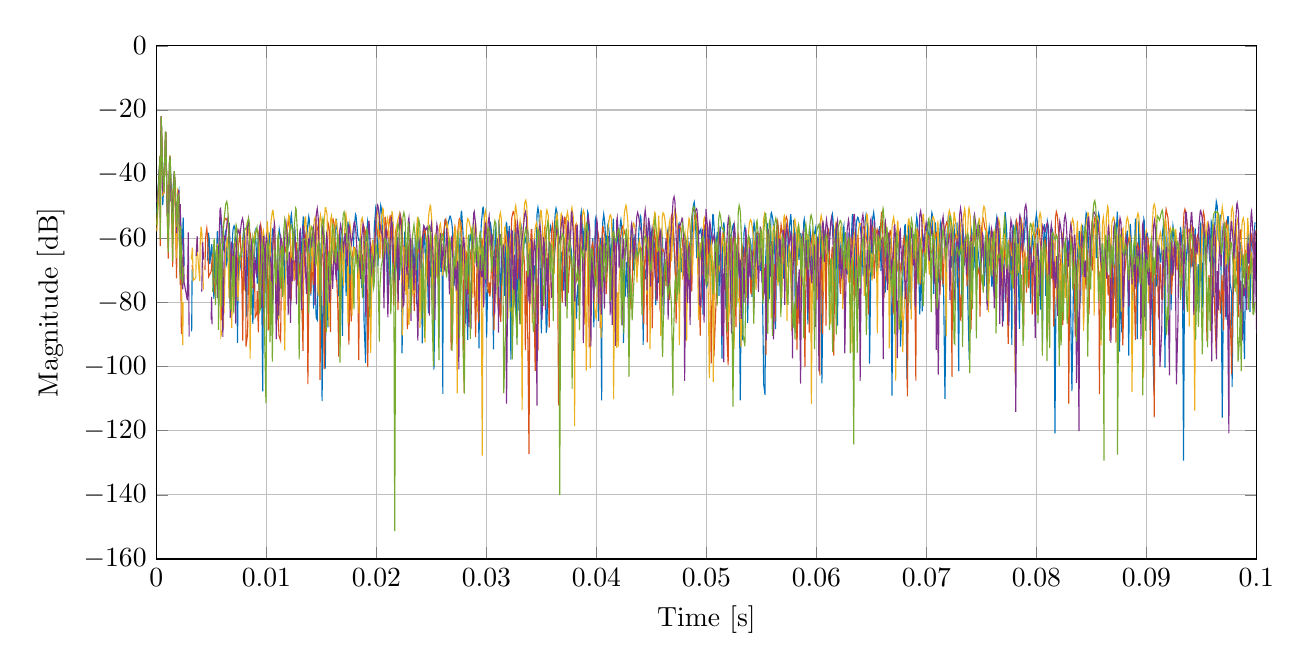
\begin{tikzpicture}

\begin{axis}[%
width=5.5in,
height=2.566in,
scaled x ticks = false,
x tick label style={/pgf/number format/fixed},
at={(1.414in,0.891in)},
scale only axis,
unbounded coords=jump,
xmin=0,
xmax=0.1,
xlabel={Time [s]},
xmajorgrids,
ymin=-160,
ymax=0,
ylabel={Magnitude [dB]},
ymajorgrids,
axis background/.style={fill=white},
title style={font=\bfseries},
%title={Time Decay}
]
\addplot [color=mycolor1,solid,forget plot]
  table[row sep=crcr]{%
2.08333333333333e-05	nan\\
4.16666666666667e-05	-52.111048310778\\
0.000166666666666667	-43.9740436319002\\
0.000333333333333333	-34.8177965827442\\
0.000354166666666667	-53.6190056426103\\
0.000354166666666667	-53.6190056426103\\
0.0004375	-21.9598363711386\\
0.0005625	-37.7606834431528\\
0.000583333333333333	-49.6288694056232\\
0.0006875	-42.2560543031998\\
0.000833333333333333	-27.0848645767238\\
0.000854166666666667	-27.0938121387821\\
0.000979166666666667	-49.8807436737733\\
0.00108333333333333	-59.9223441352537\\
0.0011875	-37.2201027543805\\
0.00125	-34.3291951406571\\
0.00135416666666667	-45.9757139957571\\
0.00147916666666667	-56.382911413555\\
0.00152083333333333	-43.9141776726352\\
0.00152083333333333	-43.9141776726352\\
0.001625	-40.042008410004\\
0.0016875	-43.2431355273656\\
0.00183333333333333	-60.9681241606569\\
0.00183333333333333	-60.9681241606569\\
0.0019375	-46.8693647146266\\
0.00204166666666667	-45.2221645426903\\
0.00214583333333333	-70.4535211157334\\
0.00216666666666667	-51.6149616670037\\
0.0023125	-64.165288874486\\
0.00235416666666667	-61.5511588605062\\
0.0024375	-53.565070295056\\
0.00252083333333333	-68.5064286025977\\
0.00252083333333333	-68.5064286025977\\
0.00266666666666667	nan\\
0.00266666666666667	nan\\
0.00289583333333333	-72.904642668182\\
0.00289583333333333	-72.904642668182\\
0.003	nan\\
0.003	nan\\
0.00320833333333333	-89.0396268578771\\
0.00325	-69.6670608974985\\
0.00333333333333333	nan\\
0.00333333333333333	nan\\
0.0035	nan\\
0.0035	nan\\
0.00364583333333333	nan\\
0.00364583333333333	nan\\
0.0038125	nan\\
0.0038125	nan\\
0.00397916666666667	nan\\
0.00397916666666667	nan\\
0.00414583333333333	nan\\
0.00414583333333333	nan\\
0.0043125	nan\\
0.0043125	nan\\
0.00464583333333333	-66.952070269611\\
0.00464583333333333	-66.952070269611\\
0.00464583333333333	-66.952070269611\\
0.00472916666666667	-58.2959288896312\\
0.0048125	-60.5931307267329\\
0.00485416666666667	-68.0794223724486\\
0.00504166666666667	-61.8026803688784\\
0.005125	-70.1443845224101\\
0.00522916666666667	-78.870829364037\\
0.0053125	-63.8012011510901\\
0.0053125	-63.8012011510901\\
0.00535416666666667	-68.5896659640424\\
0.00545833333333333	-65.4935549134102\\
0.00554166666666667	-57.7477179120546\\
0.00566666666666667	-81.2009260636828\\
0.00577083333333333	-55.761344442787\\
0.00585416666666667	-53.5416605882092\\
0.0059375	-56.2577357302003\\
0.00597916666666667	-58.9539415015357\\
0.00610416666666667	-63.8531451471768\\
0.00614583333333333	-61.9141009456243\\
0.00627083333333333	-58.0593839706459\\
0.0063125	-58.7413544861928\\
0.00639583333333333	-67.7841232832069\\
0.00645833333333333	-66.6166703808532\\
0.006625	-55.2300468372413\\
0.006625	-55.2300468372413\\
0.00679166666666667	-72.9096992394021\\
0.00679166666666667	-72.9096992394021\\
0.0069375	-58.638942876284\\
0.00697916666666667	-57.0690799271473\\
0.0070625	-56.1394046707133\\
0.00714583333333333	-57.1127041883519\\
0.00727083333333333	-63.1813781835223\\
0.00727083333333333	-63.1813781835223\\
0.007375	-92.5753078843969\\
0.00745833333333333	-66.4543104134224\\
0.0075	-65.1542648427286\\
0.00766666666666667	-68.9414396695225\\
0.00775	-66.3204732466916\\
0.00779166666666667	-63.6550975119697\\
0.00791666666666667	-57.8950515685413\\
0.00795833333333333	-57.4909363697214\\
0.00808333333333333	-61.4101564617352\\
0.008125	-65.014239665563\\
0.00820833333333333	-84.3913964822076\\
0.00827083333333333	-67.5401210436484\\
0.0084375	-60.6608842129059\\
0.0084375	-60.6608842129059\\
0.00860416666666667	-68.6525343731691\\
0.00860416666666667	-68.6525343731691\\
0.00877083333333333	-86.7182627693444\\
0.00877083333333333	-86.7182627693444\\
0.0089375	-58.3503996189966\\
0.00897916666666667	-57.7185064887609\\
0.0090625	-61.5893861763269\\
0.00916666666666666	-74.1626294665894\\
0.00925	-59.9425252546123\\
0.00925	-59.9425252546123\\
0.00939583333333333	-82.2414358792677\\
0.0094375	-63.5172219371502\\
0.00952083333333333	-57.7976918868999\\
0.00966666666666667	-107.69929084972\\
0.00975	-60.471146039021\\
0.00979166666666667	-59.0848073355518\\
0.00991666666666667	-66.2816899780258\\
0.00991666666666667	-66.2816899780258\\
0.01	-83.2384694993036\\
0.0100833333333333	-69.382102407305\\
0.01025	-58.1614130268561\\
0.01025	-58.1614130268561\\
0.0103958333333333	-78.659966600665\\
0.0104375	-64.3644685212\\
0.0105625	-57.2292963929618\\
0.0106041666666667	-57.4389958833188\\
0.0107291666666667	-61.1355190321544\\
0.0107708333333333	-62.6617442615444\\
0.0108958333333333	-69.2220796621684\\
0.011	-85.3991667784377\\
0.0110416666666667	-65.4866844897544\\
0.0110833333333333	-60.3538379061152\\
0.0111666666666667	-57.1711414785393\\
0.01125	-59.1262763800061\\
0.011375	-69.3559430679877\\
0.0114166666666667	-70.9746539468429\\
0.0115416666666667	-63.2971463445262\\
0.0115833333333333	-62.2681820493326\\
0.0117083333333333	-78.185870054493\\
0.0117291666666667	-74.8542861438093\\
0.0118958333333333	-59.1082812851507\\
0.0118958333333333	-59.1082812851507\\
0.0120208333333333	-62.3396384402111\\
0.0120625	-61.9079830499083\\
0.0122291666666667	-53.2761437613709\\
0.0122708333333333	-52.5028995257284\\
0.0123958333333333	-57.9490053815339\\
0.0124375	-67.097874268932\\
0.0125416666666667	-57.8292741595085\\
0.0125833333333333	-56.3942866017904\\
0.0127083333333333	-66.8628824569854\\
0.0127708333333333	-73.1233158076556\\
0.0128541666666667	-63.1193712248532\\
0.0128958333333333	-65.0422676184057\\
0.0129375	-72.4048294890819\\
0.0130833333333333	-66.3211400209195\\
0.013125	-71.8762952805217\\
0.0132291666666667	-59.9577490778633\\
0.0133541666666667	-53.4565553010462\\
0.0133958333333333	-53.7172714247254\\
0.0135208333333333	-59.7287434390187\\
0.0136041666666667	-63.951909199344\\
0.0136875	-59.7481136529985\\
0.0137291666666667	-56.884992279517\\
0.0138541666666667	-53.2243149389698\\
0.0138958333333333	-54.0305340746001\\
0.0140416666666667	-77.8746654022866\\
0.0140416666666667	-77.8746654022866\\
0.0141666666666667	-59.5576053975161\\
0.0142083333333333	-61.3140246411379\\
0.0142916666666667	-81.9411573286561\\
0.0143958333333333	-65.6135925586917\\
0.0145208333333333	-84.6872059910125\\
0.014625	-85.4407544579033\\
0.0146875	-74.1556791266814\\
0.0146875	-74.1556791266814\\
0.0148125	-61.5186789861121\\
0.0148541666666667	-61.603933867154\\
0.0150208333333333	-82.8897784221635\\
0.0150625	-110.772106438684\\
0.0151875	-72.3738220270998\\
0.0152291666666667	-70.4290235676362\\
0.0153541666666667	-100.606303182385\\
0.0153541666666667	-100.606303182385\\
0.0154583333333333	-72.1936353976885\\
0.0156041666666667	-87.7491540752639\\
0.0156875	-73.2013868076318\\
0.0157916666666667	-77.4373024400392\\
0.0158333333333333	-67.9974898177409\\
0.015875	-64.0529505129947\\
0.0159583333333333	-62.0225650940623\\
0.0160833333333333	-65.2961964560404\\
0.0161666666666667	-62.8831029470834\\
0.0161666666666667	-62.8831029470834\\
0.0163333333333333	-54.3557903914612\\
0.016375	-54.2032208365931\\
0.0165	-62.3646402761344\\
0.0165416666666667	-78.113175470613\\
0.0166458333333333	-58.8346612605774\\
0.0166875	-58.183753552355\\
0.0168125	-67.0010327931349\\
0.0169166666666667	-90.4436690986716\\
0.0169791666666667	-68.8442995675725\\
0.0170208333333333	-63.0786023797962\\
0.0171041666666667	-58.4773349959014\\
0.01725	-77.9505350758744\\
0.0173333333333333	-57.445562140132\\
0.0174166666666667	-54.8642361243766\\
0.0175	-58.1348941906922\\
0.0175	-58.1348941906922\\
0.0176041666666667	-81.2331799465362\\
0.0176875	-65.9063896475626\\
0.0178125	-69.9045452138529\\
0.0178541666666667	-68.2679254067739\\
0.0179791666666667	-56.6175168508517\\
0.0179791666666667	-56.6175168508517\\
0.0181041666666667	-52.5422477316158\\
0.0181458333333333	-52.8806272404262\\
0.0183125	-59.3176520761328\\
0.0183125	-59.3176520761328\\
0.0183958333333333	-60.5962203271359\\
0.0184791666666667	-60.3497039195296\\
0.0186041666666667	-69.1567240190393\\
0.0186666666666667	-75.5213852508567\\
0.01875	-65.0119785770231\\
0.0188333333333333	-69.891092188239\\
0.018875	-85.4855467125159\\
0.0190208333333333	-98.9033056569759\\
0.019125	-58.287911282984\\
0.0192083333333333	-54.732623030518\\
0.0192916666666667	-56.8444306984257\\
0.0193333333333333	-60.3684268716343\\
0.0194375	-84.5798414376857\\
0.0194791666666667	-79.599605229199\\
0.019625	-63.2791733275686\\
0.0197083333333333	-70.0795077494701\\
0.0197708333333333	-63.4095035805324\\
0.0198125	-56.362169900321\\
0.0199375	-50.7438037528893\\
0.0199791666666667	-51.6086095044044\\
0.0201041666666667	-62.884753710132\\
0.0201458333333333	-68.6491886999608\\
0.0202708333333333	-56.3246955012879\\
0.0203125	-52.7777742803338\\
0.0203958333333333	-49.7337890346514\\
0.0204791666666667	-51.1840995331472\\
0.0206041666666667	-63.5297545792679\\
0.0206875	-75.480095487511\\
0.0207708333333333	-63.1150361798449\\
0.0208125	-59.3571081508711\\
0.0208958333333333	-57.281628009858\\
0.0210208333333333	-79.6666740625991\\
0.021125	-59.7053926135665\\
0.021125	-59.7053926135665\\
0.02125	-74.6074415490915\\
0.0213125	-61.1963391171394\\
0.0214375	-54.9555009504599\\
0.0214791666666667	-56.2835768296612\\
0.0215625	-66.3184865927575\\
0.0216666666666667	-64.7381345146491\\
0.02175	-70.1569097501175\\
0.0218125	-69.0320645480348\\
0.0219375	-59.5928240237874\\
0.0219375	-59.5928240237874\\
0.0220833333333333	-73.0637301253879\\
0.0221666666666667	-62.5544202629954\\
0.02225	-65.8825503138553\\
0.0222916666666667	-72.3842214376554\\
0.0223333333333333	-95.8946786113816\\
0.0224583333333333	-70.2530157937059\\
0.0225833333333333	-58.1050091233855\\
0.022625	-57.9585276214801\\
0.02275	-71.4584000951474\\
0.0228125	-74.3549832010801\\
0.0228541666666667	-69.896266469373\\
0.0229583333333333	-75.7678645726475\\
0.0230833333333333	-61.6482335838661\\
0.023125	-63.6055317308382\\
0.0231666666666667	-70.3970329366683\\
0.0233125	-61.8747738335171\\
0.0233958333333333	-69.0316467698325\\
0.0234583333333333	-69.389326825852\\
0.0235416666666667	-59.7552089012813\\
0.0235833333333333	-60.1162958509255\\
0.0236666666666667	-80.4186936973413\\
0.0238125	-57.1309642847574\\
0.0238958333333333	-62.1212696061357\\
0.0239583333333333	-78.4103631383799\\
0.0240416666666667	-60.2068703019764\\
0.0240833333333333	-60.4092820244597\\
0.0241666666666667	-92.7997852123779\\
0.0243125	-55.9748624975703\\
0.0243958333333333	-59.2659810929925\\
0.0245	-69.6964812675586\\
0.0245833333333333	-61.3945967461279\\
0.0245833333333333	-61.3945967461279\\
0.0247291666666667	-83.319371913321\\
0.0248125	-68.1273708089018\\
0.0248541666666667	-71.9010224366383\\
0.0249166666666667	-71.8433084298515\\
0.0250416666666667	-60.2861288082898\\
0.0250833333333333	-61.096435464369\\
0.0252291666666667	-100.969926898387\\
0.0252291666666667	-100.969926898387\\
0.025375	-69.2091637938194\\
0.0254583333333333	-64.4129091348762\\
0.0255416666666667	-72.1250823743872\\
0.0256041666666667	-68.8569766183764\\
0.0257291666666667	-60.3477448082694\\
0.0257291666666667	-60.3477448082694\\
0.025875	-70.4392358736544\\
0.0259583333333333	-63.9922837115621\\
0.0260416666666667	-108.499215296894\\
0.0260625	-71.8086529212789\\
0.0262291666666667	-54.2731049476727\\
0.0262708333333333	-54.1988303491569\\
0.0263958333333333	-56.2487371503306\\
0.0264375	-56.5870521396224\\
0.0265625	-54.7482541363904\\
0.0265625	-54.7482541363904\\
0.0266875	-53.0714624478762\\
0.0267291666666667	-53.1372442191546\\
0.0268541666666667	-55.1956940556838\\
0.0268958333333333	-56.5192998662079\\
0.0270208333333333	-65.1700792132076\\
0.0270625	-74.8014316703393\\
0.0272083333333333	-62.6849454987621\\
0.0272083333333333	-62.6849454987621\\
0.027375	-82.7612057750395\\
0.027375	-82.7612057750395\\
0.0275416666666667	-65.394853202394\\
0.0275416666666667	-65.394853202394\\
0.0277083333333333	-51.7796812024415\\
0.02775	-51.6350347108753\\
0.027875	-58.2869347094643\\
0.027875	-58.2869347094643\\
0.0279791666666667	-71.7105014677704\\
0.0280625	-63.882500825233\\
0.0281875	-79.9766963561106\\
0.0283125	-91.7713094343247\\
0.0283541666666667	-72.0346732320252\\
0.0283958333333333	-65.4192303431406\\
0.0285208333333333	-58.7690022829116\\
0.0285625	-58.7501013277672\\
0.0286875	-62.3414742012781\\
0.0287708333333333	-63.8296774192487\\
0.0288541666666667	-60.902401824853\\
0.0288541666666667	-60.902401824853\\
0.0290208333333333	-56.1733269554729\\
0.0290208333333333	-56.1733269554729\\
0.0291875	-62.9384717517341\\
0.0291875	-62.9384717517341\\
0.0293333333333333	-94.3452251867561\\
0.029375	-75.153928116795\\
0.0295	-58.6378296949106\\
0.0295416666666667	-55.4440049181021\\
0.0296666666666667	-50.5908198970047\\
0.0297083333333333	-50.4136916048125\\
0.0298333333333333	-54.3119360944019\\
0.029875	-57.3837910078597\\
0.0300208333333333	-90.9026639436772\\
0.0300208333333333	-90.9026639436772\\
0.0301875	-63.419483913347\\
0.0301875	-63.419483913347\\
0.0303541666666667	-54.8131345824229\\
0.0303541666666667	-54.8131345824229\\
0.0304791666666667	-58.3092456989957\\
0.0305208333333333	-62.4471896131256\\
0.0306458333333333	-94.6357844184851\\
0.0306875	-73.4708815723489\\
0.0308125	-57.3816750760384\\
0.0308541666666667	-56.6414507577698\\
0.0309791666666667	-77.7664469629615\\
0.031	-72.2780605786322\\
0.031125	-55.1299691359179\\
0.0311666666666667	-55.6889405596294\\
0.0312916666666667	-84.5429414305775\\
0.0313958333333333	-66.2062162520025\\
0.0314375	-72.6071321396692\\
0.0315833333333333	-61.8845615853803\\
0.0316666666666667	-77.9267222422503\\
0.0316666666666667	-77.9267222422503\\
0.0318125	-55.1808883666852\\
0.0318541666666667	-55.3863791621712\\
0.032	-64.391189789455\\
0.032	-64.391189789455\\
0.0320833333333333	-56.1585703036079\\
0.0322291666666667	-97.8357655986159\\
0.0323125	-58.6814920046532\\
0.0323541666666667	-57.8066425809928\\
0.0324375	-66.3378292926789\\
0.0325	-64.1085376837165\\
0.032625	-55.86088782757\\
0.0326666666666667	-57.887144760026\\
0.03275	-91.0605011679413\\
0.0328541666666667	-60.6395159362812\\
0.0329583333333333	-82.5472088344748\\
0.033	-62.5812922968961\\
0.033125	-55.2174326136108\\
0.0331666666666667	-56.5762206187729\\
0.0333125	-68.0442432133646\\
0.0333125	-68.0442432133646\\
0.0334375	-60.5994362098871\\
0.0335208333333333	-61.2027489498795\\
0.0336458333333333	-58.6681611601902\\
0.0336458333333333	-58.6681611601902\\
0.0337291666666667	-57.249122879767\\
0.0338125	-58.5860520482856\\
0.0339375	-65.7600843469768\\
0.0339791666666667	-67.4542642459779\\
0.0341041666666667	-63.6983180734036\\
0.0341458333333333	-62.9435228460163\\
0.0342708333333333	-74.1449332839636\\
0.0343333333333333	-72.7580437882617\\
0.034375	-68.4434289523935\\
0.0344791666666667	-70.624099227779\\
0.0346041666666667	-52.502920249584\\
0.0346875	-50.4196642111809\\
0.0347708333333333	-52.3193676952971\\
0.0348125	-54.8933889601838\\
0.0349375	-77.7633538948113\\
0.035	-89.6328151281812\\
0.0351041666666667	-66.7176643343471\\
0.0351458333333333	-62.9423035437913\\
0.0352291666666667	-61.060791269831\\
0.0353125	-64.7805577900927\\
0.0354375	-89.4370899182441\\
0.0355	-88.1054345419602\\
0.035625	-68.4370950247928\\
0.035625	-68.4370950247928\\
0.03575	-58.2592420783276\\
0.0358333333333333	-56.3794554197297\\
0.0359166666666667	-58.005842561841\\
0.0359583333333333	-60.0440277702351\\
0.0360416666666667	-64.2954124513962\\
0.036125	-60.9654487707412\\
0.03625	-52.5556497638501\\
0.0363333333333333	-50.6467882825929\\
0.0364166666666667	-51.8731468063633\\
0.0364583333333333	-53.7752781241652\\
0.0365833333333333	-67.152263813057\\
0.0366666666666667	-82.2313952073381\\
0.03675	-69.8911322330386\\
0.0368333333333333	-64.2702207964671\\
0.0369166666666667	-66.5247784726584\\
0.0370208333333333	-76.3388786599295\\
0.0371041666666667	-68.8572200225383\\
0.0371458333333333	-73.1183552515281\\
0.03725	-63.4556401502907\\
0.0372916666666667	-59.5190127246632\\
0.0374166666666667	-56.2531368992099\\
0.0374583333333333	-56.7565412507788\\
0.0375833333333333	-60.4080597765621\\
0.0375833333333333	-60.4080597765621\\
0.03775	-64.5471897562287\\
0.03775	-64.5471897562287\\
0.0379166666666667	-95.0934061611474\\
0.0379166666666667	-95.0934061611474\\
0.0380208333333333	-73.3932282064926\\
0.0381041666666667	-77.1289295926568\\
0.0381875	-85.0150850334075\\
0.0382708333333333	-77.1367612344248\\
0.0383125	-74.7554553105742\\
0.0384166666666667	-75.3184030847228\\
0.0385833333333333	-52.7278170646141\\
0.038625	-51.6369661525912\\
0.03875	-56.1640807798232\\
0.03875	-56.1640807798232\\
0.0387916666666667	-63.7671311822112\\
0.0389375	-55.8190300332956\\
0.0390833333333333	-63.8309390586054\\
0.0390833333333333	-63.8309390586054\\
0.0392083333333333	-51.7484890805427\\
0.03925	-52.1330932019537\\
0.039375	-63.3541597967702\\
0.0394791666666667	-82.9508933838846\\
0.0395416666666667	-71.1849339918385\\
0.0395833333333333	-63.910616928065\\
0.0396666666666667	-60.0678376699235\\
0.0397708333333333	-87.7951764401267\\
0.0398958333333333	-54.4640684133291\\
0.0399375	-53.7447538745434\\
0.0400625	-60.3375678416738\\
0.0400625	-60.3375678416738\\
0.0401875	-85.851765726561\\
0.0402291666666667	-73.9130937702324\\
0.0403541666666667	-59.8966052036609\\
0.0404791666666667	-110.534743824305\\
0.0405416666666667	-58.9038004862074\\
0.0405833333333333	-54.8762772181309\\
0.0406666666666667	-52.4740872526299\\
0.04075	-54.7585947291255\\
0.040875	-62.09801104963\\
0.0409166666666667	-61.7817758205457\\
0.0410416666666667	-55.9012073702274\\
0.0410833333333333	-55.3022899513924\\
0.0412083333333333	-59.9751360771568\\
0.0412083333333333	-59.9751360771568\\
0.0412916666666667	-66.6459334429875\\
0.041375	-63.1158417251286\\
0.0415416666666667	-53.8979797559046\\
0.0415416666666667	-53.8979797559046\\
0.0417083333333333	-73.4788272319152\\
0.0417291666666667	-76.927090541222\\
0.0418541666666667	-58.2624632781119\\
0.0418958333333333	-58.7856339512347\\
0.0420208333333333	-62.5700963663408\\
0.0420625	-61.3699920696119\\
0.0421875	-54.9896736610798\\
0.0422291666666667	-54.1791979136858\\
0.0423541666666667	-58.4880953545163\\
0.0423958333333333	-63.5683342707567\\
0.0424583333333333	-92.6491336063769\\
0.0425416666666667	-69.5304880300145\\
0.0426458333333333	-78.2020119999443\\
0.0427291666666667	-67.3486414290402\\
0.042875	-78.5224699706943\\
0.042875	-78.5224699706943\\
0.0429583333333333	-69.7114224300351\\
0.0430625	-70.213301438398\\
0.0431875	-57.2072300736504\\
0.0432291666666667	-56.9460241572293\\
0.0433541666666667	-70.0473617866263\\
0.0433541666666667	-70.0473617866263\\
0.0435	-59.0133357503042\\
0.0435416666666667	-58.8394724809219\\
0.0436666666666667	-65.4871103591925\\
0.0437083333333333	-67.9482077097613\\
0.0438333333333333	-60.0821504188792\\
0.043875	-56.980197952122\\
0.044	-53.0335889993579\\
0.0440416666666667	-53.4116440581601\\
0.0441666666666667	-60.939727929713\\
0.0442083333333333	-67.6989364896322\\
0.04425	-93.237701403041\\
0.0443541666666667	-68.923289405939\\
0.0444791666666667	-72.7720018460815\\
0.0445208333333333	-71.0906669876785\\
0.0446458333333333	-60.2848853762254\\
0.0446875	-57.9074968923221\\
0.0448125	-55.5364599604336\\
0.0448541666666667	-56.2407206859415\\
0.0449791666666667	-62.1734316893831\\
0.0450625	-65.1364097296669\\
0.0451458333333333	-62.7615670032355\\
0.0452291666666667	-60.7229641093824\\
0.0453125	-62.9980531481612\\
0.0453958333333333	-80.8561150468016\\
0.0455	-64.0313527222714\\
0.0455416666666667	-62.8411274587434\\
0.0456666666666667	-73.9328050062999\\
0.0456666666666667	-73.9328050062999\\
0.0458125	-59.9350041049739\\
0.0458958333333333	-57.5798904827926\\
0.0459791666666667	-59.065455792161\\
0.0460208333333333	-61.607093407732\\
0.046125	-83.9469044921063\\
0.0462083333333333	-66.4444484356159\\
0.0462916666666667	-71.0103029679969\\
0.0463541666666667	-72.854708153089\\
0.0464791666666667	-57.9193863593011\\
0.0465208333333333	-57.1258141157988\\
0.0466458333333333	-60.5031957920493\\
0.0466458333333333	-60.5031957920493\\
0.0467708333333333	-65.2859387527195\\
0.0468125	-63.401712546132\\
0.0469791666666667	-56.1151281337393\\
0.0469791666666667	-56.1151281337393\\
0.0471458333333333	-69.2023905342233\\
0.0471458333333333	-69.2023905342233\\
0.0472916666666667	-75.0446037307081\\
0.0473541666666667	-67.819343320156\\
0.0474791666666667	-55.5733184915837\\
0.0475208333333333	-55.3402575812227\\
0.0476458333333333	-66.4688096902689\\
0.0477083333333333	-70.6342309025243\\
0.0477916666666667	-64.6062595561328\\
0.0478958333333333	-71.7290679867784\\
0.0479791666666667	-61.046074233917\\
0.0479791666666667	-61.046074233917\\
0.048125	-91.7902072314842\\
0.0481666666666667	-65.8358809204401\\
0.0482916666666667	-59.0336853076932\\
0.0482916666666667	-59.0336853076932\\
0.0484583333333333	-68.9332756793045\\
0.0484583333333333	-68.9332756793045\\
0.0485416666666667	-77.9664613096182\\
0.0486458333333333	-64.5193461342156\\
0.0487708333333333	-51.6120365163448\\
0.0488125	-49.7770430674985\\
0.0488958333333333	-48.7697099601659\\
0.0489791666666667	-51.610426254635\\
0.049125	-66.1772453173729\\
0.049125	-66.1772453173729\\
0.04925	-56.9297787973484\\
0.0492916666666667	-57.3190494104798\\
0.049375	-58.3031948917796\\
0.0495	-57.1553412617634\\
0.049625	-62.3071402956343\\
0.0496875	-83.8124293219814\\
0.0497708333333333	-58.801646796603\\
0.0498541666666667	-56.808523250945\\
0.0499375	-62.0888580569866\\
0.0499791666666667	-70.0275443275833\\
0.0500416666666667	-75.0734923337837\\
0.0501458333333333	-74.1943941275219\\
0.0502708333333333	-56.4148334498624\\
0.0503125	-56.1543612015576\\
0.0503958333333333	-63.78175470799\\
0.0504583333333333	-64.443727547012\\
0.0505833333333333	-52.6170582583235\\
0.050625	-52.7081018143248\\
0.05075	-59.0014482775725\\
0.0508333333333333	-63.3550620246675\\
0.0509166666666667	-60.325730436091\\
0.051	-57.9865458688801\\
0.0510833333333333	-62.3288558570694\\
0.0511458333333333	-77.9884109735364\\
0.0512708333333333	-56.3757939431772\\
0.0512708333333333	-56.3757939431772\\
0.0514166666666667	-97.5374570824204\\
0.0514583333333333	-62.3925729260549\\
0.0515833333333333	-55.0691830939375\\
0.051625	-56.3640746713164\\
0.0517708333333333	-82.1121435013862\\
0.0518125	-70.8121214342492\\
0.0519166666666667	-86.9269433872825\\
0.0519166666666667	-86.9269433872825\\
0.0520833333333333	-59.314943253348\\
0.052125	-58.9784893258279\\
0.0522083333333333	-59.3201467988916\\
0.05225	-59.2221109942112\\
0.0524166666666667	-56.0236184193138\\
0.0524583333333333	-55.686135812412\\
0.0525833333333333	-58.2750334232435\\
0.0525833333333333	-58.2750334232435\\
0.05275	-71.5816897182234\\
0.0527916666666667	-72.7436919470865\\
0.0529166666666667	-66.259466261982\\
0.0529583333333333	-65.8746136123509\\
0.0530833333333333	-110.564887150756\\
0.0530833333333333	-110.564887150756\\
0.0531875	-67.3308560871339\\
0.0532916666666667	-91.8362894380612\\
0.0534166666666667	-58.3777526226115\\
0.0534166666666667	-58.3777526226115\\
0.0535	-56.3278812863045\\
0.0535833333333333	-58.193375451677\\
0.0537083333333333	-70.1057774084365\\
0.05375	-86.3452694095191\\
0.0538958333333333	-64.0817756651716\\
0.0538958333333333	-64.0817756651716\\
0.0540208333333333	-61.2252712974897\\
0.0540625	-62.3836459518489\\
0.0541458333333333	-78.2991757151921\\
0.05425	-58.8092639419761\\
0.0543333333333333	-55.1361959391058\\
0.0544166666666667	-56.8835800299799\\
0.0545	-68.982969519186\\
0.0545625	-65.6606695135639\\
0.0546875	-58.5959254132972\\
0.0547291666666667	-59.7503979001718\\
0.0548958333333333	-70.1562575170889\\
0.0548958333333333	-70.1562575170889\\
0.0550625	-65.9665064103992\\
0.0550625	-65.9665064103992\\
0.0552083333333333	-105.509212743218\\
0.0553333333333333	-108.786447128276\\
0.0553958333333333	-66.0129525591762\\
0.0553958333333333	-66.0129525591762\\
0.0555208333333333	-55.8709656926965\\
0.0555625	-55.6296698051418\\
0.0557083333333333	-79.0323764951073\\
0.0557083333333333	-79.0323764951073\\
0.055875	-52.3372613112074\\
0.0559166666666667	-52.0192513619121\\
0.0560416666666667	-54.1484699493886\\
0.0560416666666667	-54.1484699493886\\
0.0562083333333333	-61.2351372755453\\
0.0562083333333333	-61.2351372755453\\
0.0562916666666667	-88.3124722749051\\
0.0563958333333333	-58.5122710469107\\
0.0564791666666667	-55.4337828726981\\
0.0565625	-57.146896083332\\
0.0566875	-74.0430113436521\\
0.0567916666666667	-81.6233476496053\\
0.0568541666666667	-75.8606650264225\\
0.0569375	-67.8358846415719\\
0.0570416666666667	-72.6506009458582\\
0.0570416666666667	-72.6506009458582\\
0.0571666666666667	-55.7309416321065\\
0.0572083333333333	-54.9949963040555\\
0.0573333333333333	-61.0258878053262\\
0.0574166666666667	-68.9480697683941\\
0.0575	-61.0542754056737\\
0.0575416666666667	-56.7416343100113\\
0.0576666666666667	-52.4582816249724\\
0.0577083333333333	-54.0552584448012\\
0.0578125	-72.2757018833819\\
0.0579375	-54.2978774534205\\
0.0580208333333333	-59.0191512074864\\
0.0580833333333333	-89.4570489961042\\
0.0581666666666667	-58.4024422903802\\
0.0582083333333333	-57.1484718996737\\
0.0583333333333333	-62.4448090061273\\
0.0584166666666667	-66.7348922512015\\
0.0585	-61.9494411174193\\
0.0585833333333333	-58.3477351334046\\
0.0586666666666667	-61.1201381257731\\
0.0587083333333333	-68.9041611322802\\
0.0588541666666667	-54.9558623236462\\
0.0588958333333333	-54.0787765764221\\
0.0589791666666667	-56.699944839914\\
0.0590208333333333	-60.8870504568114\\
0.059125	-71.1661896219548\\
0.0592291666666667	-86.8647031017299\\
0.0593125	-59.7200380318321\\
0.0593958333333333	-56.1957877010555\\
0.0594791666666667	-59.7495346101022\\
0.0595833333333333	-72.0444756393041\\
0.0596666666666667	-65.0527796842482\\
0.0597083333333333	-69.8342344239554\\
0.0598125	-61.2903664752369\\
0.0598541666666667	-57.9914354724829\\
0.0599375	-56.6383069335279\\
0.0600208333333333	-59.7521214040006\\
0.0601041666666667	-63.9399242315211\\
0.0601875	-61.307560212938\\
0.0603125	-55.5037275090166\\
0.0603541666666667	-55.5271141160025\\
0.0605	-105.214794578507\\
0.0605	-105.214794578507\\
0.0606666666666667	-57.3779772080543\\
0.0606666666666667	-57.3779772080543\\
0.0607916666666667	-60.9870460202388\\
0.0608333333333333	-61.6569364128772\\
0.0609583333333333	-58.6059181743705\\
0.0610416666666667	-57.336877405069\\
0.061125	-58.2847536676374\\
0.0612083333333333	-59.1318156111891\\
0.0612916666666667	-56.7028034599151\\
0.0613333333333333	-54.8943490282252\\
0.0614583333333333	-52.5014021872495\\
0.0615	-53.5726487733492\\
0.0616458333333333	-65.7929163736295\\
0.0616458333333333	-65.7929163736295\\
0.0617708333333333	-55.323097418286\\
0.0618125	-56.8083707165601\\
0.0619166666666667	-87.2501242282543\\
0.062	-61.7685426502957\\
0.0621458333333333	-71.9138256814326\\
0.0621458333333333	-71.9138256814326\\
0.0622291666666667	-60.9433326750413\\
0.062375	-67.8258825834839\\
0.0624583333333333	-56.9702360181621\\
0.0625	-56.1138627444652\\
0.062625	-66.6291611300659\\
0.0626875	-71.0011536640558\\
0.0627291666666667	-65.2551161449225\\
0.0628125	-71.3144657887031\\
0.0629583333333333	-58.4368225148986\\
0.063	-58.2013990590425\\
0.0630833333333333	-67.8891162004635\\
0.0631458333333333	-62.9401454206522\\
0.0632708333333333	-52.682238046857\\
0.0633125	-52.6857048912195\\
0.0634375	-61.505771203027\\
0.0634791666666667	-77.7113762470808\\
0.063625	-55.2290236380544\\
0.063625	-55.2290236380544\\
0.06375	-53.4460798004492\\
0.0637916666666667	-53.5796817675073\\
0.0639583333333333	-55.9437153448461\\
0.0639583333333333	-55.9437153448461\\
0.064125	-60.6398619733621\\
0.064125	-60.6398619733621\\
0.06425	-71.8389503171149\\
0.0643125	-69.2496802749246\\
0.0644375	-54.6195556765343\\
0.0644375	-54.6195556765343\\
0.0645208333333333	-52.5155062445164\\
0.0646041666666667	-53.8666573260562\\
0.0647708333333333	-70.1931118255637\\
0.0647708333333333	-70.1931118255637\\
0.0648333333333333	-99.0860516263863\\
0.0649583333333333	-67.6378163725657\\
0.0650833333333333	-55.8735644855142\\
0.065125	-53.6498784822159\\
0.0652083333333333	-51.9374092571696\\
0.0652916666666667	-54.4544366462532\\
0.0654375	-67.1082794159962\\
0.0654791666666667	-62.6894319382487\\
0.0655625	-69.1757228881748\\
0.065625	-65.9013684627119\\
0.06575	-56.2351823536755\\
0.0657916666666667	-57.4590473269785\\
0.065875	-70.2146829364207\\
0.0659375	-65.5419347852481\\
0.0660208333333333	-59.6382644818549\\
0.0661041666666667	-62.2673121816491\\
0.0662291666666667	-76.8614132294533\\
0.0662708333333333	-76.6093228488293\\
0.0663958333333333	-64.7087765445192\\
0.0664375	-63.9393863695652\\
0.0665833333333333	-74.2332735524355\\
0.0665833333333333	-74.2332735524355\\
0.0667083333333333	-60.4359148574553\\
0.06675	-60.871256554729\\
0.066875	-109.087450961713\\
0.0669791666666667	-64.376590625337\\
0.0670625	-67.535826951276\\
0.067125	-88.1185170348175\\
0.06725	-59.9604188609497\\
0.06725	-59.9604188609497\\
0.0673333333333333	-57.9569766329386\\
0.0674166666666667	-58.7564985460616\\
0.0675833333333333	-70.1272075632668\\
0.0675833333333333	-70.1272075632668\\
0.0676458333333333	-93.7716301795069\\
0.0678125	-77.8389262414299\\
0.067875	-71.1771191147298\\
0.0679166666666667	-63.7857453965473\\
0.0680416666666667	-55.9218196445023\\
0.0680833333333333	-55.8360967884015\\
0.0682291666666667	-103.909504661414\\
0.0682291666666667	-103.909504661414\\
0.0683958333333333	-55.8517361248505\\
0.0683958333333333	-55.8517361248505\\
0.0685625	-71.3955932277055\\
0.0686041666666667	-82.2018999390121\\
0.0687291666666667	-63.7505392574502\\
0.0687291666666667	-63.7505392574502\\
0.0688125	-58.7146421455994\\
0.0689583333333333	-80.7552447476887\\
0.0690416666666667	-56.5496049211186\\
0.069125	-53.3340636447095\\
0.0692083333333333	-55.5837671942404\\
0.06925	-58.8639965772437\\
0.0693958333333333	-83.6978092558424\\
0.0693958333333333	-83.6978092558424\\
0.0695416666666667	-68.6468913416614\\
0.069625	-82.8018653332479\\
0.0696875	-65.5535483746151\\
0.0697291666666667	-60.7132784658533\\
0.0698125	-58.5327956585478\\
0.0698958333333333	-66.9719715325554\\
0.0700416666666667	-56.7755002194376\\
0.0700833333333333	-55.8649890692635\\
0.0702083333333333	-59.4028734021595\\
0.07025	-60.8728198313164\\
0.070375	-56.2795887696564\\
0.070375	-56.2795887696564\\
0.0705	-52.0254535433982\\
0.0705416666666667	-52.6384908560605\\
0.0706666666666667	-77.3526227080484\\
0.0707291666666667	-59.1200144244935\\
0.0708125	-55.0294131293683\\
0.0708958333333333	-59.22574002566\\
0.071	-74.1560044481242\\
0.0710833333333333	-73.4401120968916\\
0.0711875	-59.9458759587087\\
0.0712708333333333	-55.3285523662576\\
0.0713541666666667	-57.1376942538588\\
0.0713958333333333	-60.6331555823407\\
0.0715	-75.1577770495114\\
0.0715416666666667	-69.0470794848409\\
0.0716875	-110.065077890061\\
0.0716875	-110.065077890061\\
0.0718333333333333	-63.5588456110434\\
0.071875	-58.7291788234421\\
0.072	-52.8170150986196\\
0.0720416666666667	-52.6758969005317\\
0.0721666666666667	-56.9453584629862\\
0.0722083333333333	-60.620375746593\\
0.0723125	-69.2244459790678\\
0.0723541666666667	-61.7643684503557\\
0.0724791666666667	-55.5657028147834\\
0.0725208333333333	-55.8983907763576\\
0.0726458333333333	-79.5015617331005\\
0.0727083333333333	-60.2398974850142\\
0.0727916666666667	-55.0390577346723\\
0.0729375	-101.457901579476\\
0.0730208333333333	-56.6004148441891\\
0.0730625	-55.0462268661173\\
0.0731875	-68.8559436851743\\
0.0732083333333333	-84.0989722064798\\
0.0733333333333333	-55.618576909737\\
0.0733333333333333	-55.618576909737\\
0.0734583333333333	-68.5489543240071\\
0.0735208333333333	-64.7323288320954\\
0.0736041666666667	-59.1862480822238\\
0.0736875	-64.3687408648016\\
0.0737291666666667	-74.0090374548583\\
0.0738958333333333	-97.819116372686\\
0.0739791666666667	-61.3089822050509\\
0.0740625	-56.8911472909939\\
0.0741458333333333	-58.4535132544045\\
0.0741875	-61.8575950905691\\
0.0742916666666667	-69.9803287063885\\
0.074375	-62.629130595648\\
0.0745	-71.215459981418\\
0.0745625	-75.9117504947597\\
0.0746458333333333	-64.7539642716494\\
0.0746875	-63.585086708093\\
0.0748125	-67.7969096833235\\
0.0749166666666667	-74.4738493896324\\
0.075	-63.3163723925099\\
0.075	-63.3163723925099\\
0.0750833333333333	-60.6253945205473\\
0.0751666666666667	-62.5103365039176\\
0.07525	-75.1014300317096\\
0.0753125	-69.6237354778104\\
0.0753958333333333	-62.6720528214736\\
0.0755416666666667	-80.8045722056119\\
0.075625	-59.7237503630309\\
0.0757083333333333	-56.5255751374667\\
0.0757916666666667	-58.9330862603293\\
0.0758333333333333	-62.6935532283438\\
0.0759375	-75.10140043488\\
0.0760208333333333	-69.8553237660522\\
0.0761041666666667	-75.812909068535\\
0.0761458333333333	-75.1479361751281\\
0.0763125	-55.9992874927877\\
0.0763958333333333	-53.645285897761\\
0.0764791666666667	-56.8302029839733\\
0.0764791666666667	-56.8302029839733\\
0.0765833333333333	-66.7055093603651\\
0.0766666666666667	-56.7505427392843\\
0.0767916666666667	-64.7212259773139\\
0.0768541666666667	-71.3273099740182\\
0.0768958333333333	-64.4100808565485\\
0.077	-85.8959829409815\\
0.077125	-53.1234727027349\\
0.0771666666666667	-51.8854058959738\\
0.0772916666666667	-56.9543235405698\\
0.0772916666666667	-56.9543235405698\\
0.0773958333333333	-71.7330895984557\\
0.0775208333333333	-82.8370321734584\\
0.077625	-59.7466130129635\\
0.0776666666666667	-59.0378766633308\\
0.0777708333333333	-93.2035969894017\\
0.0778125	-62.6064134606815\\
0.0778958333333333	-55.7679720490936\\
0.0780416666666667	-76.0582629858785\\
0.078125	-55.6846014498208\\
0.0781666666666667	-54.1469456554181\\
0.0782916666666667	-59.9564080913717\\
0.0782916666666667	-59.9564080913717\\
0.0784583333333333	-88.2123722311393\\
0.0784583333333333	-88.2123722311393\\
0.0785833333333333	-57.9911223722988\\
0.0786666666666667	-56.0303850462482\\
0.07875	-58.6948652661341\\
0.0788333333333333	-62.6335716225572\\
0.0789166666666667	-59.6865747535623\\
0.0789583333333333	-56.8882814018658\\
0.0790833333333333	-53.2966966288216\\
0.079125	-54.4935417490925\\
0.0792083333333333	-65.1458559244315\\
0.0792708333333333	-64.604164354631\\
0.0793541666666667	-57.7658293423414\\
0.0794791666666667	-80.2816921677761\\
0.0795833333333333	-60.064858347599\\
0.079625	-59.5456005490152\\
0.07975	-63.8096227462002\\
0.0797916666666667	-63.0717969857272\\
0.0799166666666667	-54.6267859201177\\
0.08	-52.469214077968\\
0.0800833333333333	-54.8689632918444\\
0.080125	-58.5347212433505\\
0.0802291666666667	-71.8553378902363\\
0.0802708333333333	-66.8490808210701\\
0.080375	-82.2178069489534\\
0.0804583333333333	-64.5137510188522\\
0.0805625	-92.6671428230212\\
0.0806041666666667	-64.4974540432391\\
0.0807291666666667	-55.6285295615325\\
0.0807708333333333	-56.9815242589428\\
0.0808541666666667	-77.9796634828853\\
0.0809166666666667	-59.8623664400439\\
0.081	-54.7022729146922\\
0.0810833333333333	-56.2580846231238\\
0.08125	-70.775481525813\\
0.08125	-70.775481525813\\
0.0814166666666667	-58.9321727653304\\
0.0814583333333333	-57.9676365824667\\
0.0815833333333333	-62.6867967836322\\
0.0815833333333333	-62.6867967836322\\
0.0816875	-120.804276160834\\
0.0817708333333333	-82.1608726202276\\
0.0819166666666667	-67.4753277010948\\
0.0819583333333333	-67.1043099562363\\
0.0820833333333333	-92.429982281247\\
0.0820833333333333	-92.429982281247\\
0.0821875	-72.8052397262767\\
0.0822916666666667	-76.6637800719454\\
0.082375	-63.3528947546453\\
0.0824583333333333	-60.1782279409166\\
0.0825416666666667	-62.1266684407226\\
0.082625	-74.6474770245025\\
0.0827291666666667	-64.2905167119429\\
0.0827291666666667	-64.2905167119429\\
0.0828541666666667	-60.5753585704935\\
0.0828958333333333	-61.1179855284716\\
0.0830625	-69.872015103313\\
0.0830625	-69.872015103313\\
0.0832291666666667	-107.692401694163\\
0.0832291666666667	-107.692401694163\\
0.0833958333333333	-68.5993027842871\\
0.0834375	-67.3256007787537\\
0.0835625	-70.8006529624197\\
0.0836041666666667	-72.689661355055\\
0.0837291666666667	-64.6609389274241\\
0.0837291666666667	-64.6609389274241\\
0.0838958333333333	-57.7443270166697\\
0.0838958333333333	-57.7443270166697\\
0.0840208333333333	-80.186043788939\\
0.0840416666666667	-73.1625895497147\\
0.0841666666666667	-55.9741743832219\\
0.0842083333333333	-56.1203584713389\\
0.0843541666666667	-65.6960853654616\\
0.0843958333333333	-57.7913836081153\\
0.0845208333333333	-52.1350795658206\\
0.0845625	-52.4818420041125\\
0.0846875	-57.9076592152712\\
0.0847291666666667	-60.9656932439727\\
0.0848541666666667	-68.4663465292422\\
0.0848958333333333	-67.6983609905608\\
0.0850208333333333	-61.5263354622048\\
0.0850625	-59.8354409934062\\
0.0851875	-56.4761892978199\\
0.0852708333333333	-55.7385085178454\\
0.0853541666666667	-57.2839271096257\\
0.0854375	-66.1855823066871\\
0.0855416666666667	-58.2835414478119\\
0.0855416666666667	-58.2835414478119\\
0.0856666666666667	-52.3567232170132\\
0.0857083333333333	-52.948765281124\\
0.0858333333333333	-66.3246694178859\\
0.0858958333333333	-67.6644045610473\\
0.0859791666666667	-61.424594859303\\
0.0860208333333333	-63.1715616630767\\
0.086125	-72.6287997009072\\
0.08625	-61.8455715006955\\
0.0863333333333333	-63.9983521676146\\
0.0864166666666667	-65.6680532514964\\
0.0865	-62.7799162413053\\
0.0865833333333333	-60.5810773058884\\
0.0866666666666667	-63.380093462159\\
0.0867708333333333	-72.3655530618287\\
0.0868541666666667	-62.8214883370087\\
0.0868541666666667	-62.8214883370087\\
0.0869791666666667	-72.3184732695261\\
0.0870416666666667	-78.8986835445998\\
0.0871875	-63.5113083897565\\
0.0871875	-63.5113083897565\\
0.0873541666666667	-51.7408410943027\\
0.0873541666666667	-51.7408410943027\\
0.0875208333333333	-62.972769020746\\
0.0875208333333333	-62.972769020746\\
0.0875625	-95.3166611317096\\
0.0876666666666667	-63.5005840302509\\
0.08775	-89.3088405071571\\
0.0878958333333333	-60.0261450148026\\
0.0879791666666667	-62.4484047887423\\
0.0880625	-65.5107711120812\\
0.0881458333333333	-61.6980375839567\\
0.0881875	-59.301891821969\\
0.0882708333333333	-57.6220717206155\\
0.0883958333333333	-96.6259514464842\\
0.0885	-56.6483144430931\\
0.0885416666666667	-55.5038125347271\\
0.0886666666666667	-63.744665106461\\
0.0886666666666667	-63.744665106461\\
0.0887291666666667	-79.9661510698107\\
0.088875	-67.8574686136362\\
0.089	-54.0692547410669\\
0.0890416666666667	-54.0355648372335\\
0.0891666666666667	-91.4539525603049\\
0.0891666666666667	-91.4539525603049\\
0.0893125	-54.5303923472698\\
0.0893125	-54.5303923472698\\
0.0894791666666667	-75.495061220469\\
0.0895416666666667	-80.6920976401494\\
0.0896458333333333	-61.5405275798947\\
0.0896458333333333	-61.5405275798947\\
0.0897708333333333	-54.0639786650326\\
0.0898125	-54.7377483810418\\
0.0899375	-85.8752890968704\\
0.09	-61.7057757607351\\
0.0900833333333333	-58.2395067773676\\
0.0901666666666667	-60.9880678645536\\
0.0902916666666667	-69.1562056147571\\
0.0904166666666667	-69.5702057459826\\
0.0904583333333333	-70.3458052437398\\
0.0905	-72.7383058870052\\
0.0906041666666667	-96.6202615299063\\
0.0906875	-107.661612559247\\
0.0907916666666667	-70.9573572316328\\
0.0908333333333333	-69.0901984896829\\
0.0909166666666667	-74.7211261307526\\
0.0909791666666667	-74.4266244612388\\
0.0911041666666667	-62.1393763218371\\
0.0911458333333333	-62.2833862842386\\
0.0912708333333333	-67.4374415754436\\
0.0913125	-67.443294711858\\
0.0914375	-59.2695222939509\\
0.0915208333333333	-56.59727546391\\
0.0916041666666667	-58.9834981185207\\
0.0916875	-100.300067854626\\
0.0917916666666667	-57.5476282977519\\
0.0918333333333333	-56.5813309032845\\
0.0919583333333333	-69.3105150210215\\
0.0919583333333333	-69.3105150210215\\
0.0921041666666667	-58.0195797025728\\
0.0921458333333333	-58.6538377670836\\
0.09225	-82.387603398453\\
0.0922916666666667	-63.0774267163197\\
0.0924166666666667	-56.1456804478351\\
0.0924583333333333	-57.1574877383579\\
0.092625	-68.6872137972107\\
0.092625	-68.6872137972107\\
0.0927916666666667	-60.9532101970323\\
0.0927916666666667	-60.9532101970323\\
0.0929166666666667	-69.8580026273763\\
0.0929791666666667	-67.4137399383763\\
0.0931041666666667	-56.4510264170252\\
0.0931041666666667	-56.4510264170252\\
0.0932708333333333	-63.466779179223\\
0.0932708333333333	-63.466779179223\\
0.093375	-129.359471820465\\
0.0934583333333333	-75.7478093370386\\
0.0935833333333333	-69.4617535459531\\
0.093625	-66.21940409671\\
0.09375	-61.1489873806489\\
0.0937916666666667	-61.8547298284248\\
0.0939375	-72.307521221243\\
0.0939375	-72.307521221243\\
0.0940625	-63.2879330918536\\
0.0941041666666667	-64.5596647833915\\
0.0941875	-68.8235244681323\\
0.0942708333333333	-65.7969453410575\\
0.0944375	-56.8897004025517\\
0.0944375	-56.8897004025517\\
0.0946041666666667	-78.7278962599539\\
0.094625	-80.3741421871948\\
0.0947083333333333	-68.0576921524274\\
0.0947708333333333	-83.091337563159\\
0.0948958333333333	-56.2284988477686\\
0.0949375	-55.5121905806886\\
0.0950833333333333	-81.6527402922445\\
0.0950833333333333	-81.6527402922445\\
0.0952083333333333	-55.8611213819508\\
0.09525	-55.9272776487736\\
0.0954166666666667	-66.2528239113675\\
0.0954166666666667	-66.2528239113675\\
0.0955833333333333	-58.3906810121226\\
0.095625	-57.9654158191865\\
0.0957083333333333	-64.4568310165894\\
0.0957708333333333	-67.4429755531228\\
0.0958958333333333	-54.8847160889135\\
0.0959375	-55.496597154743\\
0.0960625	-69.5099487641634\\
0.0961041666666667	-78.3639107953375\\
0.0962291666666667	-56.0743686656314\\
0.0962708333333333	-52.1102335794118\\
0.0963541666666667	-48.5424171943372\\
0.0964375	-49.8981235883721\\
0.0965208333333333	-60.2486568815224\\
0.0965833333333333	-60.8199579880001\\
0.0967083333333333	-52.6301104057175\\
0.09675	-54.1884851751395\\
0.0968958333333333	-115.900389760222\\
0.0968958333333333	-115.900389760222\\
0.0970416666666667	-62.5089317851814\\
0.097125	-57.5971982193482\\
0.0972083333333333	-62.4974701863559\\
0.09725	-85.3336307414288\\
0.0973958333333333	-53.3307273040701\\
0.0974375	-53.2770311650052\\
0.0975625	-62.7923866760762\\
0.0975625	-62.7923866760762\\
0.0976041666666667	-73.9192300448844\\
0.09775	-77.2002983105843\\
0.0977916666666667	-106.324445702389\\
0.0979166666666667	-70.2035112945575\\
0.0980416666666667	-58.0744610872146\\
0.0980833333333333	-57.7124757976165\\
0.0982083333333333	-69.8673773192133\\
0.0982708333333333	-69.6103483821997\\
0.0983541666666667	-64.17837219464\\
0.0984583333333333	-80.6905110595715\\
0.0985416666666667	-62.4213749177935\\
0.0985833333333333	-61.2040674702423\\
0.0987083333333333	-71.1723562417305\\
0.0987083333333333	-71.1723562417305\\
0.0987708333333333	-79.259275402785\\
0.0989166666666667	-97.6760911821989\\
0.099	-73.3688775607438\\
0.0990416666666667	-77.8882804425569\\
0.0991875	-60.2337146530417\\
0.0992708333333333	-58.2395642371267\\
0.0993541666666667	-63.472630727063\\
0.0994166666666667	-83.0069094057087\\
0.0995416666666667	-59.6905633143718\\
0.0995416666666667	-59.6905633143718\\
0.0997083333333333	-63.7819256621474\\
0.0997083333333333	-63.7819256621474\\
0.099875	-55.0606809366581\\
0.100020833333333	nan\\
};
\addplot [color=mycolor2,solid,forget plot]
  table[row sep=crcr]{%
2.08333333333333e-05	nan\\
4.16666666666667e-05	-55.3532768985279\\
0.000166666666666667	-45.2747828549726\\
0.000333333333333333	-34.2293475213127\\
0.000354166666666667	-62.4783617552161\\
0.000354166666666667	-62.4783617552161\\
0.0004375	-22.515461008885\\
0.0005625	-40.1752867718845\\
0.0006875	-46.0707514977223\\
0.0006875	-46.0707514977223\\
0.000833333333333333	-27.0194371561484\\
0.000854166666666667	-27.5188898990617\\
0.000979166666666667	-51.204041124998\\
0.00108333333333333	-66.3676583658506\\
0.0011875	-36.8901857900582\\
0.00122916666666667	-35.0033388301896\\
0.00135416666666667	-45.7974234264668\\
0.00135416666666667	-45.7974234264668\\
0.00147916666666667	-68.8803264373995\\
0.0015625	-46.2660943087018\\
0.001625	-39.8363404900252\\
0.0016875	-44.1746868047783\\
0.00183333333333333	-72.4722482329695\\
0.00183333333333333	-72.4722482329695\\
0.0019375	-45.421452698837\\
0.00202083333333333	-45.3751799502766\\
0.00216666666666667	-74.4999310698509\\
0.0021875	-59.4526986642991\\
0.00227083333333333	-89.8225548213342\\
0.00233333333333333	nan\\
0.00233333333333333	nan\\
0.0025	nan\\
0.0025	nan\\
0.00266666666666667	nan\\
0.00266666666666667	nan\\
0.00283333333333333	nan\\
0.00283333333333333	nan\\
0.003	nan\\
0.003	nan\\
0.00325	-68.3000060074804\\
0.00329166666666667	-69.8886525107389\\
0.00333333333333333	nan\\
0.00333333333333333	nan\\
0.0035	nan\\
0.0035	nan\\
0.00364583333333333	nan\\
0.00364583333333333	nan\\
0.0038125	nan\\
0.0038125	nan\\
0.00397916666666667	nan\\
0.00397916666666667	nan\\
0.00414583333333333	nan\\
0.00414583333333333	nan\\
0.00441666666666667	-69.931275631222\\
0.00445833333333333	-61.7008776762792\\
0.0045	-58.9119134678325\\
0.00458333333333333	-56.9253249876467\\
0.00466666666666667	-60.0203331725425\\
0.00475	-72.0266917054201\\
0.00497916666666667	-70.3198456932692\\
0.00497916666666667	-70.3198456932692\\
0.00497916666666667	-70.3198456932692\\
0.00510416666666667	-64.6906520810408\\
0.00514583333333333	-65.9006825168698\\
0.0051875	-71.489384992393\\
0.00533333333333333	-77.6175509185081\\
0.00545833333333333	-65.9286333547668\\
0.00545833333333333	-65.9286333547668\\
0.005625	-76.1148388828419\\
0.005625	-76.1148388828419\\
0.00579166666666667	-67.4643003768408\\
0.00579166666666667	-67.4643003768408\\
0.00591666666666667	-85.590543092471\\
0.00597916666666667	-64.6127402108474\\
0.00610416666666667	-56.0632196534693\\
0.00614583333333333	-54.8795269650331\\
0.00627083333333333	-53.8248276164565\\
0.0063125	-53.7561762988034\\
0.0064375	-54.4437313894554\\
0.00647916666666667	-55.0267380481205\\
0.00660416666666667	-59.4315370744805\\
0.00664583333333333	-61.7769598784602\\
0.00677083333333333	-68.0143531033628\\
0.0068125	-68.0114841044549\\
0.0069375	-66.0042843607406\\
0.00697916666666667	-65.4228706364806\\
0.00710416666666667	-63.0100100694251\\
0.00722916666666667	-61.3883101231769\\
0.00727083333333333	-62.4590574024155\\
0.00727083333333333	-62.4590574024155\\
0.00735416666666667	-72.6371224534662\\
0.00745833333333333	-62.7830649196377\\
0.00758333333333333	-58.3380376847438\\
0.007625	-59.3620150286208\\
0.00775	-69.0745758329812\\
0.00785416666666667	-91.8728550060318\\
0.00791666666666667	-65.735639971637\\
0.008	-62.1050117847158\\
0.00808333333333333	-63.6281419968582\\
0.008125	-66.9564302481552\\
0.00814583333333333	-93.8009888869444\\
0.00829166666666667	-89.833765783617\\
0.00841666666666667	-62.1935830276411\\
0.00845833333333333	-59.9884674487148\\
0.00854166666666667	-58.8149694329101\\
0.008625	-61.138842593284\\
0.00875	-75.3417901697901\\
0.00885416666666667	-75.6556347946643\\
0.00889583333333333	-72.6806286872565\\
0.0089375	-74.4248978719156\\
0.00897916666666667	-84.5499848732761\\
0.009125	-83.5130046818107\\
0.00916666666666666	-76.4508170837357\\
0.00927083333333333	-89.3329662806352\\
0.00939583333333333	-57.988685639865\\
0.00947916666666667	-55.7716317169284\\
0.0095625	-57.5031957381056\\
0.00960416666666667	-59.7772910066317\\
0.00972916666666667	-72.0895501480433\\
0.00979166666666667	-87.8949402325407\\
0.00989583333333333	-67.042378658614\\
0.00997916666666667	-64.1708543661686\\
0.0100625	-65.3627455431606\\
0.0101041666666667	-67.7134506144968\\
0.0101666666666667	-88.7481456549374\\
0.0102916666666667	-66.8964385046926\\
0.0104166666666667	-85.4051409155998\\
0.0104166666666667	-85.4051409155998\\
0.0105625	-64.3167911198013\\
0.0106041666666667	-61.7982678621839\\
0.0106875	-60.2684625690422\\
0.0107708333333333	-62.3117402002503\\
0.0108958333333333	-71.767087468392\\
0.0108958333333333	-71.767087468392\\
0.0110625	-84.3239983615569\\
0.0110625	-84.3239983615569\\
0.0111458333333333	-90.3615945547204\\
0.0112916666666667	-91.9422829465323\\
0.011375	-67.2087150467441\\
0.0114166666666667	-63.9144832790234\\
0.0115416666666667	-60.9878809296673\\
0.0115833333333333	-61.4915438359411\\
0.0117083333333333	-64.2873217581003\\
0.01175	-64.1196370083189\\
0.011875	-58.678054352498\\
0.0119166666666667	-56.7958589850405\\
0.0120416666666667	-54.234416717411\\
0.0120833333333333	-54.6916343217146\\
0.0122083333333333	-63.7232730558937\\
0.01225	-79.5778101510836\\
0.0123958333333333	-60.1584741807752\\
0.0123958333333333	-60.1584741807752\\
0.0125208333333333	-73.332582288291\\
0.0125833333333333	-68.4344542067597\\
0.0127083333333333	-61.2025464187702\\
0.0127083333333333	-61.2025464187702\\
0.0128333333333333	-74.3547573323564\\
0.0128958333333333	-74.0761503664857\\
0.0129791666666667	-67.7573145180586\\
0.0130625	-70.5743468717719\\
0.0131875	-76.2414320854326\\
0.0133333333333333	-95.0966662634555\\
0.013375	-74.5497919617938\\
0.013375	-74.5497919617938\\
0.0135416666666667	-59.1886449377967\\
0.0135833333333333	-58.7028800885243\\
0.0137083333333333	-65.0930352135177\\
0.0137083333333333	-65.0930352135177\\
0.0137708333333333	-105.494441354813\\
0.0138958333333333	-64.7734910089895\\
0.0140416666666667	-77.36491865123\\
0.0140416666666667	-77.36491865123\\
0.014125	-67.1325506172423\\
0.0142708333333333	-74.5947235297995\\
0.0143541666666667	-60.4316943722269\\
0.0143541666666667	-60.4316943722269\\
0.0145208333333333	-54.8257678183131\\
0.0145208333333333	-54.8257678183131\\
0.0146875	-57.7889622651867\\
0.0146875	-57.7889622651867\\
0.0148541666666667	-79.1764084953953\\
0.014875	-104.177372041077\\
0.015	-63.2865782886369\\
0.0150416666666667	-62.3326910483209\\
0.0151666666666667	-67.4414237466054\\
0.0152083333333333	-73.7820198324976\\
0.01525	-100.840831759059\\
0.0153541666666667	-88.4946275340357\\
0.0155	-60.7532891226688\\
0.0155416666666667	-57.9508047457277\\
0.015625	-55.4806759018092\\
0.0157083333333333	-56.684358304653\\
0.0158333333333333	-89.2958833098744\\
0.0158541666666667	-73.032911846722\\
0.0160208333333333	-54.489724422205\\
0.0160625	-54.062933337156\\
0.0161458333333333	-55.0926063594396\\
0.0161875	-56.5279229407655\\
0.0163125	-65.2981310418377\\
0.0163541666666667	-69.9981102172615\\
0.0164791666666667	-79.4549689382717\\
0.0165833333333333	-96.9346343424436\\
0.0166666666666667	-70.0660573782169\\
0.0166666666666667	-70.0660573782169\\
0.0168333333333333	-60.430097058333\\
0.016875	-60.3455826677063\\
0.017	-62.2510473340715\\
0.0170833333333333	-62.7585018586662\\
0.0171666666666667	-62.0689150128939\\
0.0172083333333333	-61.8373267048328\\
0.0173333333333333	-63.870565014221\\
0.0173333333333333	-63.870565014221\\
0.0175	-93.1463899998982\\
0.0175	-93.1463899998982\\
0.0176041666666667	-71.2647344368931\\
0.0177083333333333	-86.0127411198283\\
0.0178333333333333	-65.1739513256544\\
0.0178333333333333	-65.1739513256544\\
0.0179583333333333	-62.8160794777447\\
0.018	-62.9868440573121\\
0.018125	-63.6818504754972\\
0.0181666666666667	-63.9051474042428\\
0.0182916666666667	-67.0025650410068\\
0.0183958333333333	-98.0078447375321\\
0.0184791666666667	-67.4615135523664\\
0.0184791666666667	-67.4615135523664\\
0.0185625	-63.7620429281349\\
0.01875	-72.9277756301989\\
0.0187916666666667	-64.2128639372452\\
0.0188333333333333	-60.1477254002997\\
0.0189166666666667	-56.9494848498345\\
0.019	-57.9312900021909\\
0.019125	-68.1538515050735\\
0.0191666666666667	-76.3578129148911\\
0.0192083333333333	-100.183410754482\\
0.0193333333333333	-77.1185369193183\\
0.0194583333333333	-64.9906621486106\\
0.0195416666666667	-62.9538605817138\\
0.019625	-64.2901011918347\\
0.0196666666666667	-67.2371736849695\\
0.0197083333333333	-75.2176263316638\\
0.0198125	-62.7679460893184\\
0.0199375	-56.2092555997585\\
0.0199791666666667	-55.871866627917\\
0.0201041666666667	-58.1401765001223\\
0.0201875	-60.2332609155129\\
0.0202708333333333	-59.3155778789014\\
0.0203125	-57.9419482818057\\
0.0204375	-55.8298989455823\\
0.0204791666666667	-56.881212757545\\
0.0205625	-66.3401609092372\\
0.020625	-65.4270472917216\\
0.0207916666666667	-53.2375715586773\\
0.0207916666666667	-53.2375715586773\\
0.0209583333333333	-58.1143531585283\\
0.0210416666666667	-59.3802004163872\\
0.021125	-56.4787585907727\\
0.021125	-56.4787585907727\\
0.02125	-52.9905055889418\\
0.0212916666666667	-53.10573662083\\
0.0214583333333333	-63.5019290767528\\
0.0214583333333333	-63.5019290767528\\
0.0215833333333333	-80.9352547441857\\
0.021625	-71.2533327032755\\
0.02175	-58.1269044652846\\
0.0217916666666667	-57.0721353934301\\
0.0219166666666667	-63.5476675619159\\
0.0219583333333333	-82.3977042504131\\
0.0221041666666667	-54.1817488517821\\
0.0221875	-52.7780065918391\\
0.0222708333333333	-54.3434043622111\\
0.0222708333333333	-54.3434043622111\\
0.0224375	-63.2870151864313\\
0.0225208333333333	-64.816776680064\\
0.0226041666666667	-62.7952110177422\\
0.0226458333333333	-62.2381130422535\\
0.0227708333333333	-68.9634784633928\\
0.0228125	-88.322394734255\\
0.0229166666666667	-63.2757278390829\\
0.023	-61.177572184797\\
0.0230833333333333	-64.821840083579\\
0.023125	-69.6269389464003\\
0.0231666666666667	-80.8716795735751\\
0.0233125	-71.889580522418\\
0.0233958333333333	-75.2758733309288\\
0.0234375	-82.6175045470532\\
0.0235833333333333	-69.0014686944259\\
0.0235833333333333	-69.0014686944259\\
0.02375	-63.567490841715\\
0.0237916666666667	-63.4693023244089\\
0.0239166666666667	-64.4358827614145\\
0.024	-64.9484677430556\\
0.0240833333333333	-63.9701794499885\\
0.0240833333333333	-63.9701794499885\\
0.02425	-59.0227948490485\\
0.02425	-59.0227948490485\\
0.024375	-57.1533739831544\\
0.0244166666666667	-57.2446755442441\\
0.0245833333333333	-62.2951995047517\\
0.0245833333333333	-62.2951995047517\\
0.0247291666666667	-74.6279291171731\\
0.0247708333333333	-66.3555138981525\\
0.0248958333333333	-59.3464619838572\\
0.0249375	-59.1689302546976\\
0.0250625	-63.6228728806767\\
0.0250625	-63.6228728806767\\
0.0252291666666667	-78.5681299528607\\
0.0252291666666667	-78.5681299528607\\
0.0253958333333333	-69.0712629628139\\
0.0253958333333333	-69.0712629628139\\
0.0254791666666667	-67.8666246832599\\
0.0255625	-67.9667242882401\\
0.0257291666666667	-64.6206548759875\\
0.0257291666666667	-64.6206548759875\\
0.0258958333333333	-61.1580952044856\\
0.0258958333333333	-61.1580952044856\\
0.0260625	-60.0278606797129\\
0.0260625	-60.0278606797129\\
0.0262291666666667	-54.7462618960108\\
0.0263125	-54.0649790115098\\
0.0263958333333333	-56.8910783260899\\
0.0263958333333333	-56.8910783260899\\
0.0264791666666667	-68.8547208344631\\
0.026625	-61.3152900420789\\
0.0267083333333333	-64.6992471386726\\
0.02675	-70.756079361502\\
0.0267916666666667	-94.7759303269772\\
0.0269166666666667	-91.6208455775219\\
0.0270416666666667	-59.2515665823595\\
0.027125	-56.944148108611\\
0.0272083333333333	-60.2632299137628\\
0.0272083333333333	-60.2632299137628\\
0.0273125	-70.4647959800121\\
0.0273958333333333	-57.9056161527776\\
0.0275208333333333	-54.0957834223441\\
0.0275625	-53.8883345077182\\
0.0276875	-55.4261587761656\\
0.0277291666666667	-56.8921448150683\\
0.0278541666666667	-66.7324053993705\\
0.0278958333333333	-73.6791637096426\\
0.0279791666666667	-108.168819389862\\
0.0280625	-73.7743286945681\\
0.0281875	-64.4135414173064\\
0.0282291666666667	-64.6611557943709\\
0.0283541666666667	-74.0151086670894\\
0.0283958333333333	-77.4588206449277\\
0.0285208333333333	-66.9357183537209\\
0.0286041666666667	-63.4732805163059\\
0.0286875	-66.6021405744592\\
0.0286875	-66.6021405744592\\
0.0287916666666667	-73.6776311296743\\
0.028875	-65.7392604533592\\
0.0290208333333333	-90.8496472339641\\
0.0290208333333333	-90.8496472339641\\
0.0291458333333333	-67.8363729109269\\
0.0291875	-69.2388102129876\\
0.0292916666666667	-86.3021726941537\\
0.029375	-78.5118997297996\\
0.0295208333333333	-63.3033590449645\\
0.0296041666666667	-60.0231824430457\\
0.0296875	-63.8814441074438\\
0.02975	-80.6492923063193\\
0.0298333333333333	-58.6454306804021\\
0.029875	-56.1071779843515\\
0.0299583333333333	-54.9690949773085\\
0.0300416666666667	-57.8665934640327\\
0.0301666666666667	-77.1288925748044\\
0.0302708333333333	-73.8046501758671\\
0.0303125	-78.2175587787344\\
0.030375	-76.1141769169787\\
0.0305	-64.8789044473475\\
0.0305	-64.8789044473475\\
0.0306666666666667	-81.3113233707366\\
0.0306875	-88.6418401858527\\
0.0308125	-63.8424767051274\\
0.0308541666666667	-62.892147170165\\
0.0309791666666667	-66.5353442593121\\
0.0310208333333333	-70.5229072123313\\
0.031125	-84.4537081870048\\
0.0311666666666667	-78.5577633445922\\
0.0313125	-86.0690844955699\\
0.0313541666666667	-77.6172487518053\\
0.0314791666666667	-69.7283705082683\\
0.0315208333333333	-67.6691603485824\\
0.0316458333333333	-61.5850881535558\\
0.0317291666666667	-59.9424522194763\\
0.0318125	-61.8685486016498\\
0.0318541666666667	-64.9773142171733\\
0.0319583333333333	-77.0242865296263\\
0.0320416666666667	-69.3171207891896\\
0.0320833333333333	-73.4632300774246\\
0.0321875	-62.5251161676757\\
0.0323125	-53.5282986706979\\
0.0323125	-53.5282986706979\\
0.0324375	-51.6338383224702\\
0.0324791666666667	-51.7305167735301\\
0.0326458333333333	-54.8899438278497\\
0.0326458333333333	-54.8899438278497\\
0.0328125	-72.7449953040459\\
0.0328125	-72.7449953040459\\
0.0329583333333333	-63.1599285353304\\
0.033	-62.4938921388649\\
0.033125	-67.9690045401576\\
0.0331666666666667	-75.7482435031203\\
0.0333125	-63.8942988097434\\
0.0333541666666667	-62.9093496290031\\
0.0334791666666667	-68.697323773846\\
0.0334791666666667	-68.697323773846\\
0.0335416666666667	-94.8723729725815\\
0.0336666666666667	-70.2190007976162\\
0.0337708333333333	-92.6260499015618\\
0.033875	-127.307807038994\\
0.0339583333333333	-65.1011073044805\\
0.0339583333333333	-65.1011073044805\\
0.0340833333333333	-57.3082998033691\\
0.034125	-57.3346298399926\\
0.0342916666666667	-72.0699184471185\\
0.0342916666666667	-72.0699184471185\\
0.0344375	-101.33655223651\\
0.0344583333333333	-84.9078624418983\\
0.0345833333333333	-69.4407152049589\\
0.0346875	-94.9138608288384\\
0.0347708333333333	-64.1499284712058\\
0.0348125	-60.9711873495137\\
0.0348958333333333	-58.8593236088143\\
0.0349791666666667	-61.6005766591291\\
0.0350625	-81.6003167010144\\
0.035125	-65.6500974672751\\
0.0352916666666667	-57.398395644186\\
0.0352916666666667	-57.398395644186\\
0.0354583333333333	-61.5117925026274\\
0.0354583333333333	-61.5117925026274\\
0.035625	-72.9151336172261\\
0.035625	-72.9151336172261\\
0.0357083333333333	-87.8709452943961\\
0.0357708333333333	-76.3977510684388\\
0.0359375	-57.4302733572887\\
0.0360208333333333	-55.668264042969\\
0.0361041666666667	-59.136457469779\\
0.0361458333333333	-65.7502796575421\\
0.03625	-58.5204665474261\\
0.0363333333333333	-54.6873353291997\\
0.0364166666666667	-56.8742118490504\\
0.0364583333333333	-60.2504222677343\\
0.0365625	-112.133794469916\\
0.0366666666666667	-89.4288566376984\\
0.03675	-67.3848019057084\\
0.0368958333333333	-80.0108065755059\\
0.0369375	-64.564727979303\\
0.0369375	-64.564727979303\\
0.0371041666666667	-53.4631963779435\\
0.0371458333333333	-53.4395189318948\\
0.0372708333333333	-56.9825568473208\\
0.0372708333333333	-56.9825568473208\\
0.0374375	-77.0069906672863\\
0.0374375	-77.0069906672863\\
0.0375833333333333	-65.5444385933918\\
0.037625	-64.7855359553065\\
0.03775	-69.0880198925409\\
0.0378333333333333	-74.4542289107712\\
0.0379166666666667	-68.1683954088959\\
0.0379166666666667	-68.1683954088959\\
0.0380833333333333	-56.2468263886865\\
0.038125	-55.8612521739444\\
0.03825	-63.0604522378811\\
0.03825	-63.0604522378811\\
0.0382916666666667	-72.9837959893902\\
0.0384375	-72.6918010262847\\
0.0385833333333333	-58.9694422098591\\
0.038625	-57.5541195266758\\
0.03875	-61.9447648709\\
0.03875	-61.9447648709\\
0.038875	-86.9288971083027\\
0.0389166666666667	-80.6627614454719\\
0.0390833333333333	-58.4671468738267\\
0.039125	-57.7028075504357\\
0.03925	-63.2056661743696\\
0.03925	-63.2056661743696\\
0.0393541666666667	-94.0094766409532\\
0.0394375	-92.2690802608691\\
0.0395416666666667	-65.5470311469338\\
0.0395833333333333	-62.7048215233632\\
0.0396666666666667	-61.3064271830201\\
0.03975	-64.1574331340095\\
0.039875	-73.1541557606018\\
0.0399166666666667	-72.7232622051747\\
0.0400416666666667	-62.6373635377448\\
0.0400833333333333	-60.4292065879464\\
0.0401666666666667	-58.6997941428018\\
0.04025	-61.0045041561234\\
0.0403541666666667	-88.0063372605248\\
0.0403958333333333	-66.6459349838044\\
0.0405625	-56.4197742024639\\
0.0406041666666667	-56.3588353267683\\
0.0407291666666667	-59.2450485058411\\
0.0407291666666667	-59.2450485058411\\
0.0408958333333333	-77.3646635130684\\
0.0408958333333333	-77.3646635130684\\
0.0410416666666667	-65.2734283839048\\
0.041125	-63.7547756674389\\
0.0412083333333333	-66.4400764433431\\
0.0412083333333333	-66.4400764433431\\
0.0412916666666667	-78.1754210588815\\
0.0413958333333333	-71.6117325137177\\
0.0414791666666667	-69.7188404859783\\
0.0415625	-71.2852730655374\\
0.0416875	-66.8909115078569\\
0.0417291666666667	-63.9284517884818\\
0.0418541666666667	-57.9122884422059\\
0.0419375	-57.0268846005147\\
0.0420208333333333	-58.2939707049948\\
0.0420625	-59.3487299813505\\
0.0421458333333333	-60.5020469737546\\
0.0422291666666667	-58.9741833374491\\
0.0423541666666667	-56.2773567136135\\
0.0423958333333333	-56.1276958545207\\
0.0425208333333333	-57.601206575255\\
0.0425625	-58.2919883930822\\
0.0426875	-59.5738312314443\\
0.0427291666666667	-59.9691773423237\\
0.0428541666666667	-63.0017783027369\\
0.0428958333333333	-64.8909927869918\\
0.0430208333333333	-72.0114167394408\\
0.0430208333333333	-72.0114167394408\\
0.0431458333333333	-82.124450304977\\
0.0432083333333333	-80.009162221855\\
0.0433333333333333	-63.2580973520591\\
0.0434166666666667	-60.6759488765085\\
0.0435	-61.6473286439111\\
0.0435416666666667	-63.289394804033\\
0.0436666666666667	-69.7738130246373\\
0.0437083333333333	-70.0351330066726\\
0.0438333333333333	-65.2837642395371\\
0.043875	-64.013009915242\\
0.044	-62.7513417371882\\
0.0440416666666667	-62.8154881757949\\
0.0441666666666667	-64.1745630903241\\
0.0442083333333333	-65.8699099668469\\
0.0443125	-86.6754255661443\\
0.0443541666666667	-69.6311194990766\\
0.0444791666666667	-62.31698001752\\
0.0445208333333333	-63.6204524539554\\
0.044625	-92.463484754084\\
0.0446666666666667	-69.6088371184734\\
0.0448333333333333	-60.0073328240213\\
0.0448333333333333	-60.0073328240213\\
0.045	-64.2034352505279\\
0.045	-64.2034352505279\\
0.0450833333333333	-88.1003385765099\\
0.0451875	-61.2201628665147\\
0.0452708333333333	-57.8291268251096\\
0.0453541666666667	-59.9068275847985\\
0.0454375	-79.2223895551551\\
0.0455	-63.6167044352239\\
0.045625	-57.9741997383986\\
0.0456666666666667	-59.1939729653068\\
0.0457916666666667	-82.9028706165504\\
0.0458541666666667	-68.503568772214\\
0.0459791666666667	-63.2969532520895\\
0.0460208333333333	-63.3325662201042\\
0.0461458333333333	-64.1354736449948\\
0.0461875	-64.9706150522427\\
0.0463333333333333	-74.9443817599473\\
0.0463333333333333	-74.9443817599473\\
0.0464583333333333	-59.1021177786484\\
0.0465	-58.4034504610092\\
0.0466458333333333	-79.1996947737104\\
0.0466458333333333	-79.1996947737104\\
0.0468125	-53.0316959616366\\
0.0468541666666667	-52.7264909963125\\
0.0469791666666667	-55.842276407807\\
0.0469791666666667	-55.842276407807\\
0.0471458333333333	-65.9096860170707\\
0.0471458333333333	-65.9096860170707\\
0.04725	-86.5219579501303\\
0.0473333333333333	-64.4700501519339\\
0.0474583333333333	-57.184079583909\\
0.0475416666666667	-56.0419142840887\\
0.047625	-56.6636434272357\\
0.0476666666666667	-57.3850538286902\\
0.0477916666666667	-60.2761125438752\\
0.0478333333333333	-61.5175604563023\\
0.0479583333333333	-67.8013041835861\\
0.048	-71.2745306109264\\
0.048125	-80.2988096435156\\
0.0481666666666667	-77.2580060764388\\
0.0482916666666667	-66.7286811033827\\
0.0482916666666667	-66.7286811033827\\
0.0484583333333333	-62.3583727458514\\
0.0484583333333333	-62.3583727458514\\
0.048625	-68.6484498606881\\
0.0486666666666667	-76.5602790692765\\
0.0487708333333333	-63.5011170056994\\
0.0488125	-59.288184016688\\
0.0489375	-52.9589856910195\\
0.0490208333333333	-51.9586315459655\\
0.0491041666666667	-53.0756646080759\\
0.0491458333333333	-54.4336634567823\\
0.0492708333333333	-62.5236253692765\\
0.0493125	-67.2426803365785\\
0.0494375	-90.3442529518343\\
0.0494791666666667	-81.8850386941447\\
0.0496041666666667	-64.5522710808512\\
0.0496458333333333	-61.6892395558196\\
0.0497708333333333	-56.7724934560155\\
0.0498541666666667	-55.9836002300299\\
0.0499375	-57.6183408602645\\
0.0499791666666667	-59.7894497228595\\
0.0500625	-72.0827145947797\\
0.050125	-69.37026008838\\
0.05025	-60.4253422159367\\
0.0502916666666667	-60.9747125939328\\
0.0504375	-99.0249786393669\\
0.0504375	-99.0249786393669\\
0.0505625	-66.8923087851082\\
0.0506041666666667	-68.5917470353941\\
0.0506875	-96.7981176831181\\
0.0508958333333333	-78.3575003708592\\
0.0509375	-68.3112592740745\\
0.0509375	-68.3112592740745\\
0.0511041666666667	-59.6828190852572\\
0.0511041666666667	-59.6828190852572\\
0.0512708333333333	-62.0970289698675\\
0.0513125	-62.5233242893824\\
0.0514375	-60.8692994391349\\
0.0514375	-60.8692994391349\\
0.0515625	-58.6957386173796\\
0.0516041666666667	-58.8418019187436\\
0.0517708333333333	-70.2305734103104\\
0.0517708333333333	-70.2305734103104\\
0.0518125	-86.2339238069871\\
0.0519791666666667	-99.5949978513893\\
0.0520625	-64.7193715518368\\
0.0521041666666667	-61.4402757182327\\
0.0521875	-59.8217016435254\\
0.0523333333333333	-81.3677222066381\\
0.0524166666666667	-61.4494360034575\\
0.0525	-59.0291472967223\\
0.0525833333333333	-61.7514934078763\\
0.0525833333333333	-61.7514934078763\\
0.0526875	-87.7174780452322\\
0.0527708333333333	-62.6794073785261\\
0.0528958333333333	-58.9225932646385\\
0.0529375	-59.9126157586549\\
0.0530625	-86.4370086221853\\
0.0530833333333333	-76.5545196322827\\
0.0532083333333333	-61.5547063689917\\
0.05325	-62.0838859084403\\
0.0533958333333333	-72.7364398862415\\
0.0534375	-65.6156876589209\\
0.0535208333333333	-62.7967497391884\\
0.0536666666666667	-72.4595298588433\\
0.0537083333333333	-64.7626782416366\\
0.05375	-61.5459620255674\\
0.0538333333333333	-59.9729909540103\\
0.0539166666666667	-62.3764162841871\\
0.0540416666666667	-77.2040006952063\\
0.0541041666666667	-77.3282820597837\\
0.0542291666666667	-65.8116612390281\\
0.0542291666666667	-65.8116612390281\\
0.0543958333333333	-61.3734716363089\\
0.0543958333333333	-61.3734716363089\\
0.0545625	-58.8756533186119\\
0.0545625	-58.8756533186119\\
0.0546458333333333	-58.2363244991347\\
0.0547291666666667	-58.5747496130841\\
0.0548958333333333	-62.3370701338186\\
0.0548958333333333	-62.3370701338186\\
0.0550625	-71.6432545933172\\
0.0550625	-71.6432545933172\\
0.0551666666666667	-79.004621467818\\
0.0552916666666667	-69.1852221874448\\
0.055375	-74.6903782820449\\
0.0554166666666667	-96.3767393761249\\
0.0555208333333333	-66.8288435984184\\
0.0555625	-64.6633699106955\\
0.0556875	-62.9363954212566\\
0.0557291666666667	-62.8598511031487\\
0.0558125	-62.5904835074941\\
0.0558958333333333	-63.0443575978912\\
0.0560208333333333	-73.2249384382183\\
0.0560833333333333	-76.7596305973323\\
0.0561666666666667	-68.0667263210879\\
0.05625	-85.8589171079763\\
0.0563541666666667	-59.3887961670171\\
0.0563958333333333	-56.4686900680242\\
0.0564791666666667	-54.7609951345174\\
0.0565625	-58.5733649910946\\
0.0566666666666667	-66.7454428322867\\
0.0567083333333333	-59.604961742051\\
0.0567916666666667	-55.7290437077173\\
0.056875	-57.5861075517907\\
0.0569583333333333	-68.005651884132\\
0.0570625	-60.7826915673498\\
0.0571875	-54.1636253440058\\
0.0572708333333333	-53.3588867955614\\
0.0573541666666667	-54.3664174312299\\
0.0573541666666667	-54.3664174312299\\
0.0575208333333333	-61.5257231528637\\
0.0575208333333333	-61.5257231528637\\
0.0576875	-73.0955124845441\\
0.0577916666666667	-80.9564695969977\\
0.0578333333333333	-72.2602461327548\\
0.057875	-68.031430110528\\
0.058	-64.0620113720589\\
0.0580416666666667	-64.7249619390404\\
0.0581666666666667	-74.419841415245\\
0.0582291666666667	-94.8836843679024\\
0.0583541666666667	-75.9222835828174\\
0.0583541666666667	-75.9222835828174\\
0.0584375	-86.6013362998627\\
0.0585416666666667	-76.274478757698\\
0.0586666666666667	-72.5173955054349\\
0.0587083333333333	-72.7847639317461\\
0.0588333333333333	-75.4988097834078\\
0.058875	-77.6075381011051\\
0.0589583333333333	-100.203708577351\\
0.0590208333333333	-77.5177928359544\\
0.0591458333333333	-67.5960510245841\\
0.0591875	-66.8260828270062\\
0.0593125	-72.9814985594009\\
0.0593541666666667	-89.4099940057023\\
0.0595	-62.2007505899239\\
0.0595	-62.2007505899239\\
0.0596666666666667	-58.081134678711\\
0.0596666666666667	-58.081134678711\\
0.0598333333333333	-61.0771814856565\\
0.0598333333333333	-61.0771814856565\\
0.0599583333333333	-74.4121488495548\\
0.0600208333333333	-73.1313642158611\\
0.0601458333333333	-62.5565867535216\\
0.0601875	-62.8407459707948\\
0.0603125	-102.822408555418\\
0.0603333333333333	-76.2244664490909\\
0.0604583333333333	-64.1670575239747\\
0.0605625	-89.8344676668296\\
0.0606458333333333	-62.3353609681834\\
0.0607291666666667	-59.8198222850894\\
0.0608125	-64.6645076775898\\
0.060875	-87.2590350047571\\
0.0609583333333333	-61.2292266148605\\
0.061	-58.7470522467612\\
0.0610833333333333	-57.536204838123\\
0.0611666666666667	-60.4518252832503\\
0.06125	-72.9510245367459\\
0.0613125	-69.9602023712642\\
0.0614375	-62.7640790821837\\
0.0614791666666667	-64.2852497169699\\
0.0615833333333333	-96.6151126200234\\
0.0616666666666667	-65.788870752702\\
0.0617916666666667	-60.9029605871565\\
0.061875	-60.2356012867001\\
0.0619583333333333	-60.8865479373623\\
0.062	-61.9929971239408\\
0.062125	-73.907340074367\\
0.0621875	-77.3389309587933\\
0.0623125	-65.9970845405578\\
0.0623125	-65.9970845405578\\
0.0624791666666667	-78.3230298676527\\
0.0625416666666667	-79.100005038887\\
0.062625	-68.5734080547805\\
0.062625	-68.5734080547805\\
0.0627916666666667	-61.7990910174356\\
0.0628333333333333	-61.1598618152848\\
0.0629583333333333	-64.6231594177953\\
0.0629583333333333	-64.6231594177953\\
0.0630625	-73.8440078459259\\
0.0631458333333333	-61.9394635625574\\
0.0632291666666667	-60.0458734801961\\
0.0633125	-62.5012638687082\\
0.0634375	-79.6203951345071\\
0.0635	-76.2077889487179\\
0.063625	-63.6098133954641\\
0.063625	-63.6098133954641\\
0.06375	-59.1782011524483\\
0.0637916666666667	-59.2935075664197\\
0.0639166666666667	-70.9336739536591\\
0.0639791666666667	-68.9435430011526\\
0.0641041666666667	-57.6996445008338\\
0.0641458333333333	-56.8738775502837\\
0.0642291666666667	-56.4958924410807\\
0.0643125	-56.6070487005622\\
0.0644375	-56.9370474934761\\
0.0644375	-56.9370474934761\\
0.0646041666666667	-61.1774799311334\\
0.0646041666666667	-61.1774799311334\\
0.0647291666666667	-83.7544221290493\\
0.0647916666666667	-68.1939420795483\\
0.0649166666666667	-58.2055528382479\\
0.0649583333333333	-56.8883089582742\\
0.0650416666666667	-55.9788854765335\\
0.065125	-57.6133684915612\\
0.06525	-72.6458402532962\\
0.0653125	-68.5363126421616\\
0.0654375	-58.3008902849383\\
0.0655208333333333	-57.244128503357\\
0.0656041666666667	-58.977036272983\\
0.0656041666666667	-58.977036272983\\
0.0656875	-69.340777886092\\
0.0657916666666667	-58.1545983791782\\
0.0659166666666667	-52.179684971117\\
0.0659583333333333	-52.5308857772456\\
0.0660833333333333	-62.0810338023225\\
0.0661458333333333	-78.475451029792\\
0.0662291666666667	-62.0978323533667\\
0.0662708333333333	-61.5703064649957\\
0.0663958333333333	-72.9356696818744\\
0.0664583333333333	-72.7589385556238\\
0.0665833333333333	-60.2488892479259\\
0.0665833333333333	-60.2488892479259\\
0.0667083333333333	-57.5410095909213\\
0.06675	-57.6094703353931\\
0.0669166666666667	-66.9831466832879\\
0.0669791666666667	-83.7000285770603\\
0.0670625	-64.7338487578642\\
0.0671458333333333	-62.5861121613377\\
0.0672291666666667	-64.397786072358\\
0.0672708333333333	-66.1782413491726\\
0.0673958333333333	-69.4460431631735\\
0.0674375	-68.7192795373657\\
0.0675208333333333	-67.137132295155\\
0.0676041666666667	-67.8985721795776\\
0.0676875	-70.3277215012342\\
0.0677708333333333	-68.5122323873765\\
0.0678958333333333	-60.9774661773974\\
0.0679791666666667	-59.6287798874875\\
0.0680625	-62.9476996665785\\
0.0680625	-62.9476996665785\\
0.0682083333333333	-80.9424580785613\\
0.0682708333333333	-109.306608015513\\
0.0683958333333333	-62.0964699002088\\
0.0683958333333333	-62.0964699002088\\
0.0684791666666667	-59.4015755592469\\
0.0685625	-61.2898513214596\\
0.0686875	-68.5496129358845\\
0.0687291666666667	-68.0214675043991\\
0.0688958333333333	-60.091776195028\\
0.0688958333333333	-60.091776195028\\
0.0690416666666667	-104.3869204054\\
0.0690833333333333	-66.071597987995\\
0.0692083333333333	-57.6593098656626\\
0.06925	-58.2565057865294\\
0.069375	-67.1328635105718\\
0.0694583333333333	-74.4766829289435\\
0.0695416666666667	-68.8181861180571\\
0.0695833333333333	-65.7617545695573\\
0.0697083333333333	-62.7711194717815\\
0.0697083333333333	-62.7711194717815\\
0.069875	-65.1586405827017\\
0.069875	-65.1586405827017\\
0.0700416666666667	-60.2044331794927\\
0.0700416666666667	-60.2044331794927\\
0.070125	-58.8521436013619\\
0.0702083333333333	-59.5476702844776\\
0.070375	-63.6478973993561\\
0.070375	-63.6478973993561\\
0.0705	-64.5300224013961\\
0.0705416666666667	-64.410766401222\\
0.0707083333333333	-61.7498329495987\\
0.0707083333333333	-61.7498329495987\\
0.070875	-58.4909366223202\\
0.0709166666666667	-58.3142172852827\\
0.0710416666666667	-60.4692469207404\\
0.0710416666666667	-60.4692469207404\\
0.0711666666666667	-71.8821083951636\\
0.0712291666666667	-77.718435076733\\
0.0713541666666667	-63.5569921007063\\
0.0713958333333333	-63.1281377330285\\
0.0715208333333333	-74.6696151933509\\
0.0715208333333333	-74.6696151933509\\
0.0716666666666667	-58.9561952773654\\
0.0717083333333333	-56.8676237950817\\
0.0718333333333333	-55.0206256709917\\
0.071875	-55.2861084505679\\
0.072	-57.0264358891597\\
0.0720416666666667	-57.7018668176956\\
0.0721666666666667	-60.7563168846515\\
0.0722083333333333	-62.7468006889416\\
0.0723333333333333	-103.228510515641\\
0.0723541666666667	-78.7194504188803\\
0.0725208333333333	-61.51835500726\\
0.0725208333333333	-61.51835500726\\
0.0726875	-58.6198097663947\\
0.0727291666666667	-58.4840037534784\\
0.0728541666666667	-60.7471578517492\\
0.0728541666666667	-60.7471578517492\\
0.0730208333333333	-77.6533479435588\\
0.0730833333333333	-85.6527744112271\\
0.0731666666666667	-77.5974963776499\\
0.0732083333333333	-79.2300495793773\\
0.07325	-86.0349312670419\\
0.0733541666666667	-71.9731384110038\\
0.0734791666666667	-62.8988372503438\\
0.0735208333333333	-62.0002921292432\\
0.0736458333333333	-66.7111916077842\\
0.0736875	-74.8683014038838\\
0.0738333333333333	-62.9527900743891\\
0.073875	-62.1848043639425\\
0.074	-68.5700894475681\\
0.0740625	-88.4286508612311\\
0.0741458333333333	-64.4573384161523\\
0.0741875	-61.5391386217909\\
0.0743125	-58.6015642834394\\
0.0743541666666667	-58.9329304966109\\
0.0744791666666667	-63.3605670735517\\
0.0745208333333333	-65.8384241609839\\
0.0746458333333333	-71.0614361091996\\
0.0747708333333333	-69.3846051286296\\
0.0748125	-71.5026299369349\\
0.074875	-84.3931934875851\\
0.075	-57.786997039076\\
0.075	-57.786997039076\\
0.075125	-53.648857043503\\
0.0751666666666667	-53.7328200802764\\
0.0752916666666667	-56.186154546087\\
0.0753333333333333	-57.0372227707368\\
0.0754583333333333	-57.7968048092056\\
0.0755	-57.9574240156846\\
0.075625	-61.9232147889467\\
0.0756666666666667	-65.8148827624863\\
0.0757083333333333	-74.0982949592027\\
0.0758125	-66.2505016400044\\
0.0759791666666667	-61.2996012510269\\
0.0759791666666667	-61.2996012510269\\
0.0761458333333333	-63.8867511562264\\
0.0761458333333333	-63.8867511562264\\
0.0763125	-73.2870043840183\\
0.0763541666666667	-74.6009068668183\\
0.0764791666666667	-68.8615433211523\\
0.0764791666666667	-68.8615433211523\\
0.0766458333333333	-62.0592518396613\\
0.0766875	-61.7952857937701\\
0.0768125	-66.9283348621777\\
0.0768125	-66.9283348621777\\
0.0769166666666667	-75.1822351646689\\
0.0769583333333333	-68.2003516519485\\
0.0770833333333333	-63.8779274669698\\
0.077125	-64.3888253372836\\
0.0772916666666667	-70.0039381837917\\
0.0772916666666667	-70.0039381837917\\
0.0774375	-92.9227645535262\\
0.0774791666666667	-74.2359347129587\\
0.0776041666666667	-62.3697343962272\\
0.0776875	-61.2173722930503\\
0.0777708333333333	-64.2156155223548\\
0.0778125	-67.5686184149857\\
0.0778958333333333	-75.664852743912\\
0.0779791666666667	-68.0522435023673\\
0.0781041666666667	-56.7381272416371\\
0.0781875	-54.4721725795159\\
0.0782708333333333	-55.6114464329366\\
0.0783125	-57.461173747388\\
0.0784375	-67.1583262525009\\
0.0784791666666667	-68.8991976197506\\
0.0786041666666667	-62.8274843443549\\
0.0786875	-61.3911619010542\\
0.0787708333333333	-66.4316076561386\\
0.0788333333333333	-91.0854927738461\\
0.0789166666666667	-65.2091860629935\\
0.0789583333333333	-64.3470016943666\\
0.0791041666666667	-76.9149572690505\\
0.0791041666666667	-76.9149572690505\\
0.0791875	-65.8363182757209\\
0.0793125	-75.5795297850981\\
0.0794166666666667	-67.2454840741992\\
0.0795	-64.6095801733084\\
0.0795833333333333	-70.136249315601\\
0.079625	-83.761593940851\\
0.0797708333333333	-62.3687489736486\\
0.0797708333333333	-62.3687489736486\\
0.0799375	-58.9648899581815\\
0.0799375	-58.9648899581815\\
0.0801041666666667	-56.975278368569\\
0.0801875	-56.5842556131263\\
0.0802708333333333	-57.5929137544911\\
0.0802708333333333	-57.5929137544911\\
0.0803958333333333	-63.3236755618592\\
0.0804375	-67.1423862172216\\
0.0805416666666667	-79.8486687029552\\
0.0805833333333333	-70.8460490693734\\
0.08075	-60.9681874534381\\
0.0807916666666667	-60.3631272077212\\
0.0809166666666667	-63.3143170852153\\
0.0809166666666667	-63.3143170852153\\
0.0810208333333333	-90.5600365612959\\
0.0811041666666667	-64.2540505093897\\
0.0811875	-61.1196308143919\\
0.0812708333333333	-64.1117563522789\\
0.081375	-72.5655852602902\\
0.0814583333333333	-62.7806964844025\\
0.0815833333333333	-87.5244197833061\\
0.0815833333333333	-87.5244197833061\\
0.0817291666666667	-53.7454244369748\\
0.0818125	-51.7103603239253\\
0.0818958333333333	-52.7164131620695\\
0.0819375	-54.0948853678089\\
0.0820625	-60.4597530784578\\
0.0821041666666667	-62.8731522183762\\
0.0822291666666667	-70.628583616473\\
0.0822291666666667	-70.628583616473\\
0.0823958333333333	-87.0105896712711\\
0.0823958333333333	-87.0105896712711\\
0.0825625	-69.6558810776671\\
0.0825625	-69.6558810776671\\
0.0827291666666667	-64.7548439224216\\
0.0827291666666667	-64.7548439224216\\
0.0828958333333333	-74.8574941128775\\
0.0829375	-111.56538224639\\
0.0830416666666667	-65.654660726591\\
0.0830833333333333	-62.7897572153678\\
0.0832083333333333	-59.6024910910566\\
0.08325	-60.0205570522982\\
0.083375	-66.4957998498264\\
0.0834166666666667	-71.1162101218442\\
0.0835416666666667	-90.6929446052823\\
0.0835833333333333	-82.6284081811718\\
0.0837083333333333	-68.4250942460976\\
0.0837916666666667	-66.0575977801131\\
0.083875	-68.7067302295495\\
0.0839791666666667	-76.5771596764166\\
0.0840208333333333	-68.3306051622593\\
0.0841041666666667	-63.3123993973035\\
0.0841875	-65.0271872518571\\
0.0842916666666667	-86.3086243688547\\
0.084375	-68.4844296669234\\
0.084375	-68.4844296669234\\
0.0845208333333333	-75.9375759075751\\
0.0845625	-67.6510283711773\\
0.0846458333333333	-63.5145416700002\\
0.0847916666666667	-83.7140926924957\\
0.084875	-63.5470944552284\\
0.0849583333333333	-61.6033521930274\\
0.0850416666666667	-68.8178682571676\\
0.0851041666666667	-70.0940732656439\\
0.0851875	-57.7479557738298\\
0.0852291666666667	-55.4324295031302\\
0.0853125	-53.5823503836883\\
0.0853958333333333	-54.2304844072853\\
0.0855208333333333	-58.9371494733798\\
0.0855625	-61.5963507631069\\
0.0856875	-77.3992293247032\\
0.0857291666666667	-108.59825246214\\
0.0857916666666667	-82.5589805726306\\
0.0858958333333333	-82.985237527632\\
0.0860208333333333	-72.3455692502672\\
0.086125	-78.7914043677365\\
0.0861666666666667	-68.6606318843934\\
0.0862083333333333	-64.1351708450968\\
0.0862916666666667	-60.8146776459827\\
0.086375	-62.7710201429134\\
0.0865208333333333	-77.8079431326261\\
0.0866041666666667	-71.4542920437255\\
0.0866875	-92.0688608085617\\
0.0866875	-92.0688608085617\\
0.0868333333333333	-67.8435907028876\\
0.086875	-68.998938312502\\
0.0869583333333333	-87.8694772534385\\
0.0871041666666667	-68.245638171074\\
0.0871875	-73.7083863629482\\
0.0872291666666667	-92.5640369867033\\
0.0873333333333333	-66.247675360371\\
0.087375	-63.6921249027885\\
0.0875	-61.1152144903709\\
0.0875416666666667	-61.3757767513033\\
0.0876666666666667	-65.8475065161984\\
0.0876666666666667	-65.8475065161984\\
0.0877916666666667	-83.6609733059013\\
0.0878541666666667	-93.4120377929168\\
0.088	-72.2321671831803\\
0.088	-72.2321671831803\\
0.0881666666666667	-65.4731323085064\\
0.0881666666666667	-65.4731323085064\\
0.0883333333333333	-61.4473899129034\\
0.0883333333333333	-61.4473899129034\\
0.0884583333333333	-59.0237038551334\\
0.0885	-59.0950841289619\\
0.0886666666666667	-67.204581041931\\
0.0886666666666667	-67.204581041931\\
0.0887708333333333	-76.9233863645398\\
0.0888541666666667	-68.5714600535913\\
0.089	-91.6592058082924\\
0.089	-91.6592058082924\\
0.0891666666666667	-62.0637716495427\\
0.0892083333333333	-61.6772373224701\\
0.0892916666666667	-63.0426283229037\\
0.0893333333333333	-64.4397598720161\\
0.0894583333333333	-67.733838152059\\
0.0895	-67.8644998134388\\
0.089625	-70.2223978280455\\
0.0897083333333333	-90.1757276201827\\
0.0898125	-66.9655212480221\\
0.0898125	-66.9655212480221\\
0.0899791666666667	-60.6162806572315\\
0.0899791666666667	-60.6162806572315\\
0.0901041666666667	-59.8298646236028\\
0.0901458333333333	-60.1603906282389\\
0.0903125	-70.9821843534905\\
0.0903541666666667	-93.24387033228\\
0.0904583333333333	-66.4819198381733\\
0.0905	-65.1838096420899\\
0.090625	-69.0929289476727\\
0.0907083333333333	-115.845063165895\\
0.0908125	-66.3061541918301\\
0.0908125	-66.3061541918301\\
0.0909375	-62.3944967750153\\
0.0909791666666667	-63.2061831514679\\
0.0911041666666667	-84.1882285842495\\
0.091125	-83.8576821195625\\
0.09125	-67.9312811047646\\
0.0912916666666667	-70.2612116036518\\
0.0913958333333333	-78.9841659849596\\
0.0914791666666667	-79.0438240670633\\
0.091625	-57.5956070731931\\
0.091625	-57.5956070731931\\
0.0917916666666667	-50.9632004388759\\
0.0917916666666667	-50.9632004388759\\
0.0919583333333333	-53.57433060173\\
0.0919583333333333	-53.57433060173\\
0.092125	-61.7104425881177\\
0.092125	-61.7104425881177\\
0.0922916666666667	-77.5382123123558\\
0.0922916666666667	-77.5382123123558\\
0.0924583333333333	-64.0116143415141\\
0.0924583333333333	-64.0116143415141\\
0.0925833333333333	-60.9271713004166\\
0.092625	-61.8296228335895\\
0.0927916666666667	-69.9054023872338\\
0.0927916666666667	-69.9054023872338\\
0.0929166666666667	-65.2493318521313\\
0.0929583333333333	-64.256127664451\\
0.0930833333333333	-68.0803021186608\\
0.0931666666666667	-72.5613753622388\\
0.09325	-64.6206844293901\\
0.0932916666666667	-60.0620896013805\\
0.0934166666666667	-52.2359429411909\\
0.0935	-50.9384718013806\\
0.0935833333333333	-51.9518868882085\\
0.093625	-53.1093639773794\\
0.09375	-57.0886801354579\\
0.0938333333333333	-57.7591646177986\\
0.0939166666666667	-57.3113727511782\\
0.0939583333333333	-57.5936033943122\\
0.0940833333333333	-68.4042727420433\\
0.0941458333333333	-67.2855346964359\\
0.0942708333333333	-56.5515909360476\\
0.0942708333333333	-56.5515909360476\\
0.0944375	-70.4624244193252\\
0.0944375	-70.4624244193252\\
0.0945833333333333	-60.3307940014422\\
0.0946666666666667	-58.973305272227\\
0.09475	-59.5036255762902\\
0.09475	-59.5036255762902\\
0.0949166666666667	-68.8346707361945\\
0.0949791666666667	-70.2536291379064\\
0.0950625	-56.7132990396429\\
0.0951041666666667	-54.0140575042804\\
0.0951875	-51.8591246806009\\
0.0952708333333333	-53.2105909956626\\
0.0953958333333333	-63.3217554390388\\
0.0954375	-70.9719482933795\\
0.0955	-92.0159534923562\\
0.0956041666666667	-79.4468649271817\\
0.0956875	-71.4894090615444\\
0.0958333333333333	-78.0979912297434\\
0.0959166666666667	-67.5948645239032\\
0.0959583333333333	-66.4095009459483\\
0.0960833333333333	-69.7690880805982\\
0.0960833333333333	-69.7690880805982\\
0.09625	-86.820004464273\\
0.09625	-86.820004464273\\
0.0963541666666667	-96.0379864244237\\
0.0964375	-84.7574112712258\\
0.0965625	-77.9808247643831\\
0.0966458333333333	-76.8716233883598\\
0.0967291666666667	-83.47080990209\\
0.0967291666666667	-83.47080990209\\
0.096875	-71.5343406300527\\
0.0970208333333333	-88.5990858115077\\
0.0970625	-69.172684815002\\
0.0970625	-69.172684815002\\
0.0972291666666667	-55.3397114532812\\
0.0972708333333333	-54.8173804219068\\
0.0973958333333333	-57.9223360608079\\
0.0973958333333333	-57.9223360608079\\
0.0975625	-79.7241284382978\\
0.0975625	-79.7241284382978\\
0.0977083333333333	-94.7358052423439\\
0.09775	-102.402156697653\\
0.097875	-71.9277544782122\\
0.0979166666666667	-67.1590163229207\\
0.0980416666666667	-59.480226957832\\
0.098125	-57.9778210251663\\
0.0982083333333333	-59.1740525918321\\
0.09825	-61.2454020642896\\
0.0983541666666667	-84.6005368083159\\
0.0983958333333333	-66.3258716816843\\
0.0985208333333333	-57.5362022769469\\
0.0985625	-57.4675870501605\\
0.0986875	-63.3005337258442\\
0.0987291666666667	-67.2311719930743\\
0.0988125	-72.3626164518641\\
0.0988958333333333	-66.8405792346384\\
0.0989791666666667	-63.583822341822\\
0.0990625	-66.8619782233315\\
0.0991666666666667	-74.3546840206141\\
0.09925	-68.5376315505717\\
0.0993541666666667	-73.8966389471848\\
0.0993958333333333	-65.1135293896874\\
0.0995208333333333	-58.6570030610734\\
0.0995625	-58.9672711988549\\
0.0996875	-62.9776519520461\\
0.0997291666666667	-63.5665163815782\\
0.0998541666666667	-59.2573443481215\\
0.100020833333333	-57.3382452527152\\
};
\addplot [color=mycolor3,solid,forget plot]
  table[row sep=crcr]{%
2.08333333333333e-05	nan\\
4.16666666666667e-05	-57.8359820234314\\
0.000166666666666667	-49.5564281404008\\
0.000333333333333333	-35.6043109173467\\
0.000354166666666667	-47.1346796096948\\
0.000354166666666667	-47.1346796096948\\
0.0004375	-21.8673628817586\\
0.0005625	-37.6362619126018\\
0.000583333333333333	-46.9552576945675\\
0.0006875	-43.7295235139674\\
0.000833333333333333	-26.7529299173373\\
0.000854166666666667	-27.3542355571172\\
0.000979166666666667	-50.9336266224258\\
0.00116666666666667	-40.6755031596766\\
0.0011875	-35.7252437963813\\
0.00122916666666667	-33.9926476233378\\
0.00133333333333333	-48.6115221814067\\
0.00135416666666667	-43.4418891334175\\
0.00147916666666667	-54.046305109957\\
0.00154166666666667	-44.1260150550797\\
0.00164583333333333	-40.2378886438046\\
0.0016875	-43.7605497561354\\
0.0018125	-66.1163959436424\\
0.00189583333333333	-56.3502110366248\\
0.00191666666666667	-44.908729378402\\
0.00204166666666667	-46.2893881849535\\
0.002125	-60.6500516036255\\
0.0021875	-56.670891511077\\
0.00222916666666667	-65.4061260829368\\
0.00239583333333333	-93.2786909820445\\
0.0024375	-79.9095141988658\\
0.0025	nan\\
0.0025	nan\\
0.00279166666666667	-72.7315020557779\\
0.00283333333333333	-69.602971320924\\
0.00283333333333333	-69.602971320924\\
0.00283333333333333	-69.602971320924\\
0.003	nan\\
0.003	nan\\
0.0031875	-66.6151708508364\\
0.00327083333333333	-62.9056255650082\\
0.00335416666666667	-73.1447196469639\\
0.00335416666666667	-73.1447196469639\\
0.00358333333333333	-72.3218418187368\\
0.003625	-64.3596100664998\\
0.00370833333333333	-60.1204250175783\\
0.00375	-64.9846152966523\\
0.0039375	-73.3202556300712\\
0.00397916666666667	-62.143725665068\\
0.00397916666666667	-62.143725665068\\
0.0040625	-56.3636740938155\\
0.00414583333333333	-58.641578594639\\
0.00427083333333333	-76.0263363502041\\
0.0043125	nan\\
0.0043125	nan\\
0.00447916666666667	nan\\
0.00447916666666667	nan\\
0.00464583333333333	nan\\
0.00464583333333333	nan\\
0.0048125	nan\\
0.0048125	nan\\
0.00497916666666667	nan\\
0.00497916666666667	nan\\
0.00514583333333333	nan\\
0.00514583333333333	nan\\
0.00533333333333333	-74.3460839028456\\
0.00545833333333333	-64.0884503845313\\
0.00545833333333333	-64.0884503845313\\
0.00554166666666667	-61.9811855114269\\
0.005625	-62.2799671593471\\
0.00579166666666667	-69.4402133235021\\
0.00579166666666667	-69.4402133235021\\
0.005875	-90.3858307342648\\
0.00610416666666667	-87.3865153646366\\
0.006125	-69.4397779452427\\
0.00614583333333333	-83.426136321378\\
0.00627083333333333	-66.5725411306764\\
0.0063125	-63.1853350835762\\
0.0064375	-60.1653288634808\\
0.00647916666666667	-61.0554806035122\\
0.00660416666666667	-78.5503416479037\\
0.006625	-75.5488909461557\\
0.00670833333333333	-67.8404767459648\\
0.00685416666666667	-87.9420875649683\\
0.0069375	-66.5266352573682\\
0.00702083333333333	-64.5064173038671\\
0.00710416666666667	-69.1743465226069\\
0.00714583333333333	-79.2742819680841\\
0.00725	-70.0861969398425\\
0.00729166666666667	-68.2787315150359\\
0.00741666666666667	-79.5375554393991\\
0.00747916666666667	-75.1469905205635\\
0.00760416666666667	-65.9877455369571\\
0.00760416666666667	-65.9877455369571\\
0.00777083333333333	-64.4114535313614\\
0.00777083333333333	-64.4114535313614\\
0.0079375	-60.4777744499425\\
0.0079375	-60.4777744499425\\
0.00804166666666667	-76.4863670335423\\
0.008125	-60.3991051746924\\
0.00825	-55.0490439947159\\
0.00829166666666667	-54.9010453698859\\
0.00841666666666667	-58.9241397667204\\
0.00845833333333333	-62.7479835700649\\
0.00852083333333333	-97.517287274862\\
0.00860416666666667	-70.8106990746171\\
0.0086875	-75.1033079093792\\
0.00879166666666667	-72.066057568904\\
0.00891666666666667	-59.3678507928051\\
0.00895833333333333	-58.2816590566162\\
0.00908333333333333	-57.4055435815109\\
0.00916666666666666	-57.3015672405056\\
0.00925	-57.6661999077371\\
0.00925	-57.6661999077371\\
0.00941666666666667	-66.0139272774315\\
0.00945833333333333	-75.3190801429293\\
0.0095625	-65.3326348317102\\
0.00960416666666667	-61.3254970909637\\
0.00972916666666667	-57.7777182337877\\
0.00977083333333333	-58.6205392939829\\
0.00991666666666667	-66.4194604409769\\
0.00991666666666667	-66.4194604409769\\
0.0100833333333333	-54.6318673318841\\
0.0100833333333333	-54.6318673318841\\
0.01025	-63.3650419455513\\
0.0102916666666667	-88.2601541883355\\
0.0103958333333333	-56.5932751837675\\
0.0104375	-54.2618496634929\\
0.0105625	-51.3231743882186\\
0.0106041666666667	-51.3762042681551\\
0.0107291666666667	-55.4874931742853\\
0.0107708333333333	-59.1244254063581\\
0.0108125	-65.8131633558263\\
0.0109166666666667	-76.4649259901896\\
0.011	-66.9984737579311\\
0.0111458333333333	-85.0744615699199\\
0.0112291666666667	-65.4681196080555\\
0.0112291666666667	-65.4681196080555\\
0.0113125	-63.2865002510941\\
0.0113958333333333	-65.0434956773067\\
0.0115625	-73.4540350095351\\
0.0115625	-73.4540350095351\\
0.0116666666666667	-94.9417847770421\\
0.01175	-70.76455259196\\
0.011875	-57.9636463116509\\
0.0119166666666667	-55.5733046178477\\
0.0120416666666667	-52.710674694719\\
0.0120833333333333	-53.2172206499337\\
0.0122083333333333	-61.2522581397853\\
0.0123125	-74.3814247275694\\
0.0123958333333333	-66.1060633693642\\
0.0123958333333333	-66.1060633693642\\
0.0125208333333333	-70.6836653921059\\
0.0126041666666667	-72.8716944994464\\
0.0126875	-68.3364773006067\\
0.0127291666666667	-66.1750281331398\\
0.0128125	-64.4573890676974\\
0.0128958333333333	-67.2258425259825\\
0.0129791666666667	-84.8713662024197\\
0.0130416666666667	-74.8246872802407\\
0.0131666666666667	-64.984811975478\\
0.0133125	-79.6921452683636\\
0.0133541666666667	-65.1844071381086\\
0.0133958333333333	-59.6533616776275\\
0.0135208333333333	-53.5087007800342\\
0.0135625	-53.3885257256955\\
0.0136875	-59.0340651045513\\
0.0137916666666667	-69.804189743036\\
0.013875	-58.4136480255025\\
0.013875	-58.4136480255025\\
0.0139583333333333	-56.2022163919031\\
0.0140416666666667	-58.0231811814987\\
0.0141875	-70.4876582156125\\
0.0142291666666667	-61.7476663182982\\
0.0143541666666667	-54.2413565545227\\
0.0144375	-53.4244015282456\\
0.0145208333333333	-54.5938309972614\\
0.0145208333333333	-54.5938309972614\\
0.0146875	-76.0126894184846\\
0.0147083333333333	-77.8980152731918\\
0.0148333333333333	-54.7411815116013\\
0.0149166666666667	-52.7352371926056\\
0.015	-54.6633215813953\\
0.0150833333333333	-64.800108879719\\
0.0151875	-57.5428704741011\\
0.0151875	-57.5428704741011\\
0.0153541666666667	-50.4938095660772\\
0.0153958333333333	-50.4368525577924\\
0.0155208333333333	-52.7770366901671\\
0.0155208333333333	-52.7770366901671\\
0.0156875	-87.4592274400566\\
0.0156875	-87.4592274400566\\
0.0158333333333333	-54.1743498133381\\
0.0159166666666667	-52.9875292849484\\
0.016	-55.9195004615572\\
0.0160416666666667	-59.8927571739752\\
0.0160833333333333	-69.3651773269234\\
0.0161875	-58.2524954559332\\
0.0163125	-54.2249085402178\\
0.0163541666666667	-54.5135738721592\\
0.0164791666666667	-57.6574201839986\\
0.0165208333333333	-59.1376527054737\\
0.0166458333333333	-66.3335954652804\\
0.0167083333333333	-90.9551303459137\\
0.0168333333333333	-61.4379863132172\\
0.016875	-60.3365285090535\\
0.017	-73.7189156449055\\
0.0170208333333333	-74.8287950377655\\
0.0171458333333333	-54.0235794385343\\
0.0172291666666667	-52.3748377729051\\
0.0173125	-55.1257285274174\\
0.0174166666666667	-86.5168264924264\\
0.0175	-57.9876341230099\\
0.0175	-57.9876341230099\\
0.0175833333333333	-55.3629292550073\\
0.0176666666666667	-57.5766083041478\\
0.0177916666666667	-84.132051132669\\
0.0178541666666667	-67.0368953506145\\
0.0179375	-63.0508269756607\\
0.0179791666666667	-63.2578904550988\\
0.0181458333333333	-67.7638030071287\\
0.0181458333333333	-67.7638030071287\\
0.0182708333333333	-66.6590741703324\\
0.0183125	-67.1681568566808\\
0.0184166666666667	-83.3578397489755\\
0.0185	-61.7249790148479\\
0.018625	-54.4746039096365\\
0.0187083333333333	-53.6234737095024\\
0.0187916666666667	-55.5564306270902\\
0.0188333333333333	-57.930881752402\\
0.0189166666666667	-69.9509655690899\\
0.0189791666666667	-69.2846440893813\\
0.0191041666666667	-61.0699608102475\\
0.0191458333333333	-61.0712208458818\\
0.0193125	-64.0651345940905\\
0.0193125	-64.0651345940905\\
0.0194791666666667	-95.7352388774134\\
0.0194791666666667	-95.7352388774134\\
0.019625	-61.6634645187668\\
0.0196666666666667	-60.4649642414219\\
0.0197916666666667	-67.119587372799\\
0.0198541666666667	-68.8579966198792\\
0.0199375	-55.856448964451\\
0.0199791666666667	-53.4256546073939\\
0.0200625	-51.6484475471667\\
0.0201458333333333	-53.0935725139357\\
0.0202708333333333	-65.9259251442991\\
0.0203333333333333	-66.0806147785357\\
0.0204583333333333	-53.3439230677673\\
0.0204583333333333	-53.3439230677673\\
0.0205833333333333	-50.7298238954525\\
0.020625	-51.0210277163022\\
0.0207916666666667	-64.9972507209476\\
0.0207916666666667	-64.9972507209476\\
0.0209375	-55.4589279358983\\
0.0210208333333333	-53.7709637358142\\
0.0211041666666667	-55.7983956116325\\
0.0211875	-65.6093516419926\\
0.0212916666666667	-57.4711098736991\\
0.0212916666666667	-57.4711098736991\\
0.0214166666666667	-51.7564936416554\\
0.0214583333333333	-51.9105406716102\\
0.0215833333333333	-58.5237493695864\\
0.0216875	-68.4604725309403\\
0.0217708333333333	-58.7641217270695\\
0.0217708333333333	-58.7641217270695\\
0.0219375	-54.499788463108\\
0.0219375	-54.499788463108\\
0.0221041666666667	-52.2903014896305\\
0.0221041666666667	-52.2903014896305\\
0.0222708333333333	-59.0407824932996\\
0.0222708333333333	-59.0407824932996\\
0.0223541666666667	-90.3120278250571\\
0.0225	-62.7169333044515\\
0.0225833333333333	-67.6487343375312\\
0.0226875	-77.6714077205929\\
0.0227708333333333	-70.0969844881174\\
0.0227708333333333	-70.0969844881174\\
0.0228958333333333	-85.2844188026133\\
0.0229583333333333	-87.0788259531855\\
0.0231041666666667	-72.9733268514646\\
0.0231041666666667	-72.9733268514646\\
0.0231875	-66.5085991601163\\
0.0232708333333333	-69.1937908170998\\
0.0233125	-77.3580474444853\\
0.0235	-76.6498971639802\\
0.0235625	-67.1772953631774\\
0.0236041666666667	-60.2380366982807\\
0.0237291666666667	-53.5403524423138\\
0.0237708333333333	-53.6789349563237\\
0.0238958333333333	-62.050459261486\\
0.0239583333333333	-87.9060720521103\\
0.0240833333333333	-60.0315209828565\\
0.024125	-59.7849292869017\\
0.02425	-63.8666984462624\\
0.02425	-63.8666984462624\\
0.0244166666666667	-92.4363830023961\\
0.0244166666666667	-92.4363830023961\\
0.0245625	-66.699400497033\\
0.0246041666666667	-62.9700615416852\\
0.0247291666666667	-54.2249745449578\\
0.0247708333333333	-52.2964863210818\\
0.0248958333333333	-49.752950273446\\
0.0249375	-50.0510356020625\\
0.0250625	-55.6814312237319\\
0.0250625	-55.6814312237319\\
0.0251666666666667	-85.0356299888976\\
0.02525	-60.874725781504\\
0.0253333333333333	-59.0524335564243\\
0.0254166666666667	-61.7305832049777\\
0.0255	-72.5309469015093\\
0.0255625	-70.2940606268367\\
0.0257291666666667	-56.4665952488959\\
0.0258125	-55.520184688495\\
0.0258958333333333	-57.8005530686046\\
0.0258958333333333	-57.8005530686046\\
0.0260416666666667	-71.7272237905655\\
0.026125	-62.9295249416966\\
0.0262083333333333	-69.0848237241769\\
0.0262708333333333	-69.2275975075735\\
0.0263958333333333	-56.0642969056591\\
0.0264375	-55.4623267012661\\
0.0265625	-59.1906985841834\\
0.0265625	-59.1906985841834\\
0.0267291666666667	-75.4091795262659\\
0.0267291666666667	-75.4091795262659\\
0.0268541666666667	-84.0622955033773\\
0.0269166666666667	-80.1655646372091\\
0.0270416666666667	-60.456046459065\\
0.0270416666666667	-60.456046459065\\
0.0271666666666667	-56.5297059015643\\
0.0272083333333333	-57.1370107401538\\
0.0273541666666667	-108.335343759674\\
0.0273958333333333	-65.4203743089898\\
0.0275208333333333	-55.4171825270959\\
0.0275625	-54.8317695623234\\
0.0276875	-58.1030011652501\\
0.0277291666666667	-61.7384176009005\\
0.0278333333333333	-71.6567618459085\\
0.0279166666666667	-62.7079890833432\\
0.0280416666666667	-73.523901568942\\
0.0280416666666667	-73.523901568942\\
0.0281875	-57.4360434940986\\
0.0282291666666667	-55.4745074284427\\
0.0283125	-53.9194792115812\\
0.0283958333333333	-54.3101101145871\\
0.0285208333333333	-56.2589452989688\\
0.0285625	-56.9360385266716\\
0.0286875	-61.0323548112584\\
0.0286875	-61.0323548112584\\
0.0287708333333333	-78.6454037885004\\
0.028875	-58.8467748111232\\
0.029	-54.9135584711085\\
0.0290416666666667	-55.6810844317415\\
0.0291666666666667	-66.3641378163888\\
0.0292083333333333	-83.1249562865768\\
0.0293541666666667	-63.0762431322257\\
0.0293958333333333	-62.8766461288883\\
0.0295208333333333	-65.5042585235378\\
0.0295208333333333	-65.5042585235378\\
0.029625	-127.790839022745\\
0.0297083333333333	-61.8671770779253\\
0.0298333333333333	-52.8105324573841\\
0.0299166666666667	-51.4668629486395\\
0.03	-53.4637430735562\\
0.0300416666666667	-56.2250767866195\\
0.030125	-75.8722079079917\\
0.0301875	-62.7028955613962\\
0.0303125	-57.5812802990018\\
0.0303541666666667	-58.4070765273262\\
0.0304791666666667	-64.1272493673524\\
0.0305208333333333	-66.1158496957345\\
0.0306458333333333	-69.9937486118037\\
0.0307291666666667	-78.9548426594043\\
0.0308333333333333	-69.5758858763527\\
0.0309166666666667	-66.1588877248966\\
0.031	-80.2179347888694\\
0.0310208333333333	-80.4815518416204\\
0.0311458333333333	-55.4660419671327\\
0.0311875	-53.4108515322427\\
0.0312708333333333	-52.0201487157847\\
0.0313541666666667	-53.7402157184479\\
0.0314791666666667	-67.9428799712128\\
0.0315416666666667	-66.6729420676613\\
0.0316666666666667	-56.6600070785497\\
0.0317083333333333	-56.399859926777\\
0.0318333333333333	-60.2705261176081\\
0.0318333333333333	-60.2705261176081\\
0.0319583333333333	-85.1457218321726\\
0.0320208333333333	-68.6165454501909\\
0.0321458333333333	-60.4232861660291\\
0.0322291666666667	-59.649761412367\\
0.0323125	-61.7323383831401\\
0.0323125	-61.7323383831401\\
0.0324166666666667	-86.996015841297\\
0.0325	-58.2545048476356\\
0.032625	-50.4747029327167\\
0.0326666666666667	-49.7909182764732\\
0.0327916666666667	-53.1483395602738\\
0.032875	-66.5134629065215\\
0.0329791666666667	-56.9912572707965\\
0.0330625	-54.5708725157712\\
0.0331458333333333	-57.2098723710148\\
0.0331458333333333	-57.2098723710148\\
0.03325	-113.589664371204\\
0.0333333333333333	-57.7600537311296\\
0.0334583333333333	-49.9230579498698\\
0.0335	-48.7721666345451\\
0.0335833333333333	-48.1038682886867\\
0.0336666666666667	-49.7752738661459\\
0.0337916666666667	-59.4897367489667\\
0.0338333333333333	-69.2429113632977\\
0.0339375	-61.9413099820804\\
0.0339791666666667	-60.7725392757414\\
0.0341041666666667	-67.8704959865414\\
0.0341666666666667	-86.3574306547779\\
0.0342916666666667	-62.4694773228258\\
0.0342916666666667	-62.4694773228258\\
0.0344583333333333	-56.4210611274249\\
0.0345416666666667	-55.1787825351024\\
0.034625	-56.8001676605934\\
0.034625	-56.8001676605934\\
0.0347083333333333	-67.6956938962537\\
0.0348125	-57.0023033696729\\
0.0349375	-51.307978424694\\
0.0349791666666667	-51.3532753784499\\
0.0351041666666667	-56.0724557111228\\
0.0351875	-68.0306578226495\\
0.0352916666666667	-59.7122612130054\\
0.0352916666666667	-59.7122612130054\\
0.0354583333333333	-51.5330592316286\\
0.0355	-51.1241293763187\\
0.035625	-52.9533248832069\\
0.035625	-52.9533248832069\\
0.03575	-62.5341629022816\\
0.0357916666666667	-72.8484832176629\\
0.0359375	-61.225063309972\\
0.0359791666666667	-60.7859091143651\\
0.0361041666666667	-69.8522192374095\\
0.0361666666666667	-70.4119355627895\\
0.03625	-57.6261023718226\\
0.0362916666666667	-54.9841351691715\\
0.0364166666666667	-52.5435939604912\\
0.0364583333333333	-53.3919505413978\\
0.0366041666666667	-86.7791394422607\\
0.0366041666666667	-86.7791394422607\\
0.0367708333333333	-52.7295980094672\\
0.0368125	-52.3734648724261\\
0.0369375	-55.364518450758\\
0.0369375	-55.364518450758\\
0.0370625	-68.0115665114401\\
0.037125	-69.9466908119593\\
0.03725	-54.997653352522\\
0.0372916666666667	-53.21367337358\\
0.037375	-51.8357789928733\\
0.0374583333333333	-53.7814402913212\\
0.0375416666666667	-63.7507304558105\\
0.0376041666666667	-63.1695131074584\\
0.0377291666666667	-51.1612757729778\\
0.0377708333333333	-50.4163264401966\\
0.0378958333333333	-53.2346793664415\\
0.0379375	-56.4641645014394\\
0.0380208333333333	-118.57091502292\\
0.0380833333333333	-60.5552397646387\\
0.0382083333333333	-55.7268182651585\\
0.03825	-56.2667349463866\\
0.0384166666666667	-65.2530967525128\\
0.0384166666666667	-65.2530967525128\\
0.0385208333333333	-75.8988385386107\\
0.0386041666666667	-60.6523759723449\\
0.0387291666666667	-52.8905136800162\\
0.0388125	-51.2957587117686\\
0.0388958333333333	-52.2112619917496\\
0.0389375	-53.7747625626414\\
0.0390833333333333	-101.273507827482\\
0.0390833333333333	-101.273507827482\\
0.03925	-58.1721172323238\\
0.03925	-58.1721172323238\\
0.039375	-65.2266201505289\\
0.0394375	-100.550465621485\\
0.0395625	-63.5280054186009\\
0.0395625	-63.5280054186009\\
0.0397291666666667	-71.3407016045559\\
0.0397291666666667	-71.3407016045559\\
0.0398541666666667	-81.9781415020209\\
0.0399791666666667	-85.3373632602851\\
0.0400416666666667	-80.0068028701716\\
0.0400833333333333	-72.5069345230944\\
0.0402083333333333	-66.2133730946995\\
0.04025	-66.903442237468\\
0.040375	-77.4639801125304\\
0.0404166666666667	-90.9975097147481\\
0.0405625	-67.6995667049694\\
0.0405625	-67.6995667049694\\
0.0407291666666667	-59.4395996530746\\
0.0407291666666667	-59.4395996530746\\
0.0408958333333333	-70.6580661818587\\
0.0408958333333333	-70.6580661818587\\
0.0410416666666667	-58.2986288970397\\
0.0410833333333333	-56.136937989507\\
0.0412083333333333	-53.0908416504886\\
0.0412916666666667	-52.7175686462474\\
0.041375	-53.9456046734495\\
0.041375	-53.9456046734495\\
0.0415416666666667	-72.3760584992374\\
0.0415625	-110.17653950172\\
0.0416875	-63.2938181631375\\
0.0417291666666667	-64.3052494985696\\
0.0418541666666667	-94.158027331379\\
0.0419166666666667	-76.8672241299623\\
0.042	-93.7858968074181\\
0.0420625	-73.5004121662226\\
0.0421875	-67.3192777296851\\
0.0422708333333333	-68.6674596290212\\
0.0423541666666667	-65.7317386615736\\
0.0423958333333333	-62.2302122455119\\
0.0425208333333333	-53.3825797835034\\
0.0425625	-51.6361260969612\\
0.0426875	-49.7060625981705\\
0.0427291666666667	-50.103123604123\\
0.0428541666666667	-54.7589535173884\\
0.0428958333333333	-57.7131573947277\\
0.0430208333333333	-69.741027602938\\
0.0430625	-70.1609894133852\\
0.0431875	-60.6625424646071\\
0.0431875	-60.6625424646071\\
0.0433541666666667	-55.3908366949369\\
0.0433958333333333	-55.2427688395015\\
0.0435208333333333	-57.0523556511683\\
0.0435208333333333	-57.0523556511683\\
0.0436875	-73.8065263642981\\
0.0436875	-73.8065263642981\\
0.0438333333333333	-61.8498728787983\\
0.0439166666666667	-60.554958943357\\
0.044	-63.1906840340937\\
0.0440833333333333	-75.187927870047\\
0.0441875	-62.5758556436576\\
0.0441875	-62.5758556436576\\
0.0443541666666667	-54.1204856300356\\
0.0443541666666667	-54.1204856300356\\
0.0445208333333333	-62.4960468011167\\
0.0445833333333333	-77.5382006483955\\
0.0446666666666667	-60.565789816065\\
0.0447083333333333	-59.5198281192605\\
0.0448333333333333	-68.1751949223768\\
0.044875	-94.542683580573\\
0.0449791666666667	-62.9445337038034\\
0.0450208333333333	-61.0164875322099\\
0.0451458333333333	-56.5586277198673\\
0.0451875	-54.9344158435487\\
0.0453125	-51.9581243353195\\
0.0453541666666667	-52.2199161489962\\
0.0454791666666667	-62.6061362763946\\
0.0455416666666667	-64.3218133828426\\
0.0456666666666667	-52.9113033897486\\
0.0456666666666667	-52.9113033897486\\
0.0458333333333333	-67.9990493155675\\
0.0458541666666667	-90.5365439715818\\
0.0459791666666667	-53.8197936589462\\
0.0460625	-52.0444196725897\\
0.0461458333333333	-52.5450436504487\\
0.0461875	-53.2515332098516\\
0.0463125	-56.6390081474346\\
0.0463541666666667	-58.6629589405744\\
0.0464375	-69.1987446094753\\
0.0465	-67.2779817549573\\
0.046625	-55.2727403446914\\
0.0466666666666667	-54.5713708885201\\
0.0467916666666667	-59.5832172058887\\
0.0468333333333333	-67.2150915979147\\
0.0469791666666667	-54.569501763188\\
0.0469791666666667	-54.569501763188\\
0.0471458333333333	-50.8697914561432\\
0.0471458333333333	-50.8697914561432\\
0.0473125	-53.8343977412253\\
0.0473125	-53.8343977412253\\
0.0474791666666667	-65.8735241415476\\
0.0475416666666667	-93.3400201345076\\
0.047625	-65.4481554759637\\
0.0477083333333333	-62.9426031139894\\
0.0477916666666667	-66.3108275328213\\
0.0478333333333333	-72.8688924303417\\
0.0479791666666667	-60.5859537899912\\
0.0480625	-58.4666395917844\\
0.0481458333333333	-62.6101379366959\\
0.0482083333333333	-92.0233762530913\\
0.0482916666666667	-58.5664820949026\\
0.0482916666666667	-58.5664820949026\\
0.0484166666666667	-53.8136662665353\\
0.0484583333333333	-54.06736035664\\
0.048625	-62.6442083731257\\
0.048625	-62.6442083731257\\
0.0487291666666667	-71.5488557799342\\
0.0488125	-59.9050153794719\\
0.0489375	-54.5075509417962\\
0.0490208333333333	-53.5771919515918\\
0.0491041666666667	-54.7961763374789\\
0.0491458333333333	-56.495024720091\\
0.0492916666666667	-85.5578978963643\\
0.0492916666666667	-85.5578978963643\\
0.0494166666666667	-61.5227484228337\\
0.0494583333333333	-61.5403886129587\\
0.0496041666666667	-71.3918399995271\\
0.0496458333333333	-62.1692813400471\\
0.0497708333333333	-54.1025684802647\\
0.0498125	-53.5179165737767\\
0.0499375	-54.9936651066304\\
0.0499791666666667	-56.2607353520653\\
0.0501041666666667	-61.6111252841144\\
0.0501041666666667	-61.6111252841144\\
0.0502708333333333	-103.593132400311\\
0.0502708333333333	-103.593132400311\\
0.0504166666666667	-62.5217362007234\\
0.0504583333333333	-61.5498947312688\\
0.0505833333333333	-68.8453459222846\\
0.050625	-104.754669822587\\
0.0507708333333333	-60.7094511783623\\
0.0507708333333333	-60.7094511783623\\
0.0509375	-73.4414354408518\\
0.051	-76.2692709926816\\
0.0510833333333333	-68.7043090457996\\
0.051125	-68.733131522441\\
0.0512083333333333	-69.8586793407005\\
0.0512916666666667	-66.6791256716867\\
0.0514166666666667	-59.9278148850615\\
0.0514583333333333	-59.0913282773696\\
0.0515833333333333	-64.2308908510951\\
0.051625	-73.0943973009078\\
0.0517708333333333	-60.9827177226056\\
0.0518125	-60.7009118790365\\
0.0518958333333333	-64.6033291569863\\
0.0519375	-69.9184452296491\\
0.052	-86.0942921943585\\
0.0521875	-78.6579862253041\\
0.0522291666666667	-69.3306103554068\\
0.0522708333333333	-65.2552889425723\\
0.0523541666666667	-62.6946669422238\\
0.0524375	-65.6996239090703\\
0.0525208333333333	-94.4830682240316\\
0.0525833333333333	-68.5194002065346\\
0.0527083333333333	-63.3374266092536\\
0.05275	-64.4455653007544\\
0.052875	-79.5163027597807\\
0.0529791666666667	-78.9717851843213\\
0.0530625	-83.6903411464356\\
0.0531458333333333	-93.9206971221515\\
0.0532291666666667	-77.9825952951246\\
0.0532708333333333	-72.7068063021969\\
0.0533958333333333	-66.0699871938529\\
0.0534375	-66.104603815877\\
0.0535625	-75.6454740385263\\
0.053625	-78.5861441888759\\
0.0537083333333333	-65.5951844726157\\
0.05375	-62.4458264609397\\
0.053875	-56.3996643943479\\
0.0539166666666667	-55.2559042421642\\
0.054	-54.2024773819114\\
0.0540833333333333	-54.6700234180007\\
0.0542083333333333	-57.5433286178475\\
0.05425	-58.919807257679\\
0.054375	-64.925794202367\\
0.0544166666666667	-68.6008859321851\\
0.0545208333333333	-76.0678841102677\\
0.0545625	-68.8775460181091\\
0.0547291666666667	-59.8884668635159\\
0.0548125	-58.9993537472591\\
0.0548958333333333	-60.7094117010049\\
0.0548958333333333	-60.7094117010049\\
0.0550416666666667	-71.1941633554521\\
0.0550833333333333	-62.6071662378501\\
0.0552083333333333	-53.8006391563337\\
0.0552916666666667	-52.2158368258467\\
0.055375	-53.0654704825296\\
0.0554166666666667	-54.535271993847\\
0.0555416666666667	-68.4842607240848\\
0.0556041666666667	-69.669126260925\\
0.0556875	-60.823144125209\\
0.0557291666666667	-59.976952951707\\
0.0558541666666667	-66.8826003909056\\
0.0558958333333333	-85.0289840385649\\
0.0560416666666667	-57.7677068752062\\
0.0560416666666667	-57.7677068752062\\
0.056125	-56.3063678538061\\
0.0562083333333333	-57.3489127281529\\
0.056375	-62.3872497991014\\
0.056375	-62.3872497991014\\
0.0565	-74.8391776708181\\
0.0565625	-70.9354273781202\\
0.0566875	-59.2771086265215\\
0.0567291666666667	-59.0521011071723\\
0.0568541666666667	-78.6086697939858\\
0.056875	-75.1519519232134\\
0.0570416666666667	-53.3617453580533\\
0.0570833333333333	-52.9376342938016\\
0.0571666666666667	-54.5334685063173\\
0.0572083333333333	-56.6774096466749\\
0.0573333333333333	-85.7219199894691\\
0.0573541666666667	-76.825515912144\\
0.0575208333333333	-61.8739030794621\\
0.0575208333333333	-61.8739030794621\\
0.0576875	-69.5638479266833\\
0.05775	-88.947748365885\\
0.0578333333333333	-63.4708364596606\\
0.057875	-59.7791330007344\\
0.058	-54.5109363453661\\
0.0580416666666667	-54.0802381564141\\
0.0581666666666667	-57.1902660300696\\
0.05825	-68.6999608332383\\
0.0583541666666667	-60.6872681747453\\
0.0583541666666667	-60.6872681747453\\
0.0584375	-57.3131151253812\\
0.0585208333333333	-59.6939764474889\\
0.058625	-83.1757764766899\\
0.0587083333333333	-61.1662810205634\\
0.0587916666666667	-58.8481382176232\\
0.058875	-62.3542066694808\\
0.0589791666666667	-73.4722342749393\\
0.0590208333333333	-64.8440526078162\\
0.0591458333333333	-59.0859337562154\\
0.0591875	-58.9649297219052\\
0.0593125	-59.8996011355759\\
0.0593541666666667	-60.5028544014138\\
0.0594791666666667	-66.8844406230593\\
0.0595416666666667	-111.669306567476\\
0.0596666666666667	-60.7062193032765\\
0.0596666666666667	-60.7062193032765\\
0.05975	-58.5006003898186\\
0.0598333333333333	-59.3912492372967\\
0.06	-68.1718001100495\\
0.06	-68.1718001100495\\
0.0600833333333333	-79.1339491333549\\
0.0601875	-68.3269205175872\\
0.0603125	-56.6898252050938\\
0.0603541666666667	-54.6942951194985\\
0.0604375	-52.9127986523373\\
0.0605208333333333	-54.3905019069081\\
0.0606666666666667	-76.654561817506\\
0.0606666666666667	-76.654561817506\\
0.0607916666666667	-57.7119304135439\\
0.0608333333333333	-57.500608316754\\
0.0609583333333333	-61.6533421020274\\
0.061	-63.9968526614178\\
0.061125	-71.0242603051661\\
0.0611666666666667	-73.6927424141367\\
0.0613125	-86.8500302000601\\
0.0613125	-86.8500302000601\\
0.0614583333333333	-72.6538986165546\\
0.0615	-67.1218366400467\\
0.061625	-58.7744012677697\\
0.0616666666666667	-57.2838827004452\\
0.0617916666666667	-55.0204466237037\\
0.0618333333333333	-55.1053781408613\\
0.0619583333333333	-60.5504363967305\\
0.0620625	-68.1270631410947\\
0.0621458333333333	-58.2862474036183\\
0.0621875	-57.1914788873197\\
0.0623125	-61.760815585141\\
0.0623125	-61.760815585141\\
0.0623958333333333	-82.0474289518579\\
0.0625	-66.3698819948924\\
0.062625	-63.8919009746685\\
0.062625	-63.8919009746685\\
0.06275	-61.8266331006505\\
0.0627916666666667	-61.8392648305187\\
0.0629166666666667	-73.8526907493405\\
0.0629791666666667	-68.7245477901275\\
0.0631041666666667	-59.877161995949\\
0.0631458333333333	-60.9529481968992\\
0.06325	-95.5670826606478\\
0.0632916666666667	-66.7553263007645\\
0.0634583333333333	-57.8412922985346\\
0.0634583333333333	-57.8412922985346\\
0.063625	-69.1103128036463\\
0.0636875	-73.0086536500386\\
0.0637708333333333	-60.2466087378782\\
0.0638125	-57.8705942624292\\
0.0639375	-55.3374404134352\\
0.0639791666666667	-55.3450952222706\\
0.0641041666666667	-56.0246401634775\\
0.0641458333333333	-56.3073237858891\\
0.0642708333333333	-59.7521179115997\\
0.0643541666666667	-77.9445529313366\\
0.0644166666666667	-62.255191308887\\
0.0644583333333333	-57.3060958665583\\
0.0645833333333333	-52.465733258956\\
0.064625	-52.599450685636\\
0.06475	-57.8313105000431\\
0.0647916666666667	-62.2327483757959\\
0.0648333333333333	-71.0469623161337\\
0.0649791666666667	-64.6203890105173\\
0.0650625	-73.1994055029545\\
0.065125	-69.1719699088312\\
0.06525	-57.3540905627337\\
0.0652916666666667	-56.6634721924867\\
0.0654166666666667	-59.9276761837196\\
0.0654583333333333	-63.2491354012099\\
0.0655416666666667	-89.6791816633841\\
0.0656041666666667	-68.6743103655032\\
0.0657708333333333	-60.4111331141251\\
0.0658541666666667	-59.5658566282325\\
0.0659375	-60.4512251851232\\
0.0659375	-60.4512251851232\\
0.0660625	-71.2818460616956\\
0.066125	-71.4086334245439\\
0.06625	-57.8669636246348\\
0.06625	-57.8669636246348\\
0.0663333333333333	-56.360328572158\\
0.0664166666666667	-57.8337531989136\\
0.0665833333333333	-72.5813716497043\\
0.066625	-94.2914009404524\\
0.0667291666666667	-66.2717713955731\\
0.0667708333333333	-62.7656388417315\\
0.0668958333333333	-55.5853147008334\\
0.0670208333333333	-53.4660457745549\\
0.0670625	-54.2505903063785\\
0.0671041666666667	-56.1517668573432\\
0.0672083333333333	-104.400492222081\\
0.06725	-63.4212268761232\\
0.067375	-54.8047968499956\\
0.0674166666666667	-55.0199495309292\\
0.0675833333333333	-68.8505001759534\\
0.0675833333333333	-68.8505001759534\\
0.0676458333333333	-85.6311106282762\\
0.0677708333333333	-76.57685435975\\
0.0678541666666667	-95.515021449546\\
0.0679166666666667	-86.1705716622925\\
0.0680416666666667	-77.9799193792974\\
0.0680833333333333	-73.187161176195\\
0.0682083333333333	-60.9794748620602\\
0.06825	-58.2947916117133\\
0.068375	-54.0967533512741\\
0.0684166666666667	-53.9587423952874\\
0.0685416666666667	-58.8302858902116\\
0.068625	-85.3107968450152\\
0.0687291666666667	-59.9532964568628\\
0.0687708333333333	-58.9290888012452\\
0.0688958333333333	-67.7843609682746\\
0.0689583333333333	-70.8327082213738\\
0.0690416666666667	-59.6894777710846\\
0.069125	-57.6356865024753\\
0.0692083333333333	-58.688298837211\\
0.06925	-59.9251585781355\\
0.069375	-66.8928196969192\\
0.0694166666666667	-73.8892247911994\\
0.0695625	-58.1913732746452\\
0.0695625	-58.1913732746452\\
0.0696875	-52.694947594149\\
0.0697291666666667	-52.5937643174319\\
0.0698541666666667	-58.8575816154192\\
0.0698958333333333	-66.4862774580631\\
0.0700416666666667	-58.0894789071218\\
0.0700833333333333	-57.6795374903928\\
0.0702083333333333	-67.4611816384455\\
0.0702708333333333	-71.4338934538278\\
0.0703541666666667	-59.6063802784282\\
0.0703958333333333	-57.4666347854993\\
0.0705208333333333	-54.1981359238244\\
0.0706041666666667	-53.2931724017557\\
0.0706875	-53.8483917714514\\
0.0707291666666667	-55.0451503218384\\
0.070875	-81.6301360667504\\
0.070875	-81.6301360667504\\
0.0710416666666667	-54.4548869794229\\
0.0710416666666667	-54.4548869794229\\
0.0712083333333333	-65.941337899559\\
0.0712708333333333	-66.4472322563585\\
0.0713541666666667	-56.7454923570177\\
0.0713958333333333	-55.3483294836209\\
0.0714375	-54.8437821525421\\
0.0715208333333333	-55.3398683065734\\
0.0716875	-59.6348395849444\\
0.0716875	-59.6348395849444\\
0.0718125	-90.5592819073043\\
0.071875	-62.9009095960958\\
0.072	-53.0210555970829\\
0.0720833333333333	-51.323100959364\\
0.0721666666666667	-52.4151828592137\\
0.0722083333333333	-54.3259367742666\\
0.0722916666666667	-65.5870945685265\\
0.0723541666666667	-63.5061180383049\\
0.0725208333333333	-51.705087593777\\
0.0725208333333333	-51.705087593777\\
0.0726875	-55.9687618739362\\
0.0726875	-55.9687618739362\\
0.0728333333333333	-67.4198144023849\\
0.072875	-60.3667714427248\\
0.073	-54.2551617010459\\
0.0730416666666667	-54.1195152171179\\
0.0731666666666667	-59.8687964623876\\
0.0732083333333333	-68.1117180421153\\
0.0733125	-56.8925889021589\\
0.0733541666666667	-53.6307134550775\\
0.0734791666666667	-50.8106668900701\\
0.0735208333333333	-51.6153333399384\\
0.0736458333333333	-65.8065695580902\\
0.0737083333333333	-61.2176900970972\\
0.0738333333333333	-51.0722652173046\\
0.073875	-50.5209559388732\\
0.074	-53.573353246912\\
0.074	-53.573353246912\\
0.074125	-79.2916500481359\\
0.0741875	-62.2377503124342\\
0.0743125	-55.7281424598711\\
0.0743541666666667	-55.7536145340949\\
0.0744791666666667	-61.086041434142\\
0.0745833333333333	-71.5087484007587\\
0.0746666666666667	-58.3856089661661\\
0.0746666666666667	-58.3856089661661\\
0.0747916666666667	-53.7845492942524\\
0.0748333333333333	-53.8878363419154\\
0.0749583333333333	-62.9682211427097\\
0.0750208333333333	-66.3751364096079\\
0.0751458333333333	-51.6569933952535\\
0.0751458333333333	-51.6569933952535\\
0.0752291666666667	-50.0620279892693\\
0.0753125	-50.7644713340789\\
0.0754791666666667	-56.5678467743264\\
0.0754791666666667	-56.5678467743264\\
0.0756458333333333	-83.0713015396122\\
0.0756458333333333	-83.0713015396122\\
0.0757916666666667	-59.1822602035959\\
0.075875	-57.8229133805409\\
0.0759583333333333	-61.2932442236075\\
0.0760625	-71.9400262545322\\
0.0761458333333333	-59.4747111158385\\
0.0762291666666667	-57.5693431240817\\
0.0763125	-61.669942759459\\
0.0763541666666667	-69.6649127760344\\
0.0764583333333333	-58.9131052857309\\
0.0765	-56.0042943955308\\
0.0765833333333333	-54.2469884827964\\
0.0766666666666667	-55.9074567789576\\
0.0767916666666667	-63.3195299620921\\
0.0768333333333333	-67.6271084857561\\
0.076875	-75.8169092023152\\
0.0769791666666667	-65.5403570478707\\
0.0771041666666667	-58.7934940962314\\
0.0771458333333333	-58.9317562894791\\
0.0772708333333333	-70.534363148394\\
0.0773333333333333	-71.0700136182699\\
0.0774583333333333	-60.7427626353305\\
0.0775	-60.5761208163187\\
0.077625	-63.0745242103945\\
0.077625	-63.0745242103945\\
0.07775	-65.3134896286369\\
0.077875	-64.9358539978124\\
0.0779583333333333	-66.702052497697\\
0.0779583333333333	-66.702052497697\\
0.0780625	-102.443119907161\\
0.0781458333333333	-65.6433324508433\\
0.0782291666666667	-61.6416067570907\\
0.0784166666666667	-70.7925043970997\\
0.0784583333333333	-62.4014307750878\\
0.0784583333333333	-62.4014307750878\\
0.0785833333333333	-54.6884421473881\\
0.078625	-54.126368410003\\
0.07875	-56.4498211482834\\
0.0787916666666667	-58.6405660578943\\
0.0789166666666667	-70.1693359201418\\
0.079	-74.1778465198594\\
0.0790833333333333	-68.3301254868323\\
0.079125	-66.1423195793278\\
0.0792083333333333	-64.827956991271\\
0.0792916666666667	-66.9336604167689\\
0.079375	-68.6811768453004\\
0.0794583333333333	-64.4844835808461\\
0.0795833333333333	-57.1512675890344\\
0.0797083333333333	-55.2415443340742\\
0.07975	-55.9121770492662\\
0.0797916666666667	-57.3425965360339\\
0.0799166666666667	-68.6259075492641\\
0.08	-83.3982320123089\\
0.0800833333333333	-68.2589072664094\\
0.080125	-62.4482864769667\\
0.08025	-53.6545336989073\\
0.0803333333333333	-52.0393487847456\\
0.0804166666666667	-53.1801998381887\\
0.0804166666666667	-53.1801998381887\\
0.0805833333333333	-71.5507248051425\\
0.0805833333333333	-71.5507248051425\\
0.0807291666666667	-63.4354647374368\\
0.0807708333333333	-63.140892813567\\
0.0808958333333333	-65.7798684182582\\
0.0809375	-66.8714316743318\\
0.0810625	-70.4843572920476\\
0.0811458333333333	-81.2669996764089\\
0.08125	-68.4571544387609\\
0.08125	-68.4571544387609\\
0.0814166666666667	-59.9937457014377\\
0.0814583333333333	-59.6799191562294\\
0.0815833333333333	-61.4626904968501\\
0.0815833333333333	-61.4626904968501\\
0.08175	-69.7265788388498\\
0.08175	-69.7265788388498\\
0.0818958333333333	-82.4410808930869\\
0.0819375	-74.8169095555818\\
0.0820625	-67.9996218475683\\
0.0821041666666667	-68.4657032267232\\
0.0822083333333333	-88.0429927263178\\
0.08225	-69.6171694217743\\
0.082375	-58.9893284528068\\
0.0824166666666667	-58.4596193818237\\
0.0825416666666667	-63.5378937552058\\
0.0825833333333333	-68.5209407731315\\
0.082625	-78.6789916041819\\
0.0827291666666667	-73.9158245779477\\
0.0828541666666667	-84.5314351472028\\
0.0829166666666667	-80.5171248983973\\
0.0830416666666667	-64.4677695518267\\
0.0830833333333333	-61.3293002345988\\
0.0832083333333333	-55.3540961068596\\
0.0832916666666667	-53.9938592362879\\
0.083375	-54.9648190074901\\
0.0834166666666667	-56.7173677175891\\
0.0835	-67.346387272231\\
0.0835625	-65.8811892090795\\
0.0837291666666667	-54.5026376892781\\
0.0837291666666667	-54.5026376892781\\
0.0838958333333333	-71.5221026891606\\
0.0839166666666667	-86.2488006887728\\
0.0840416666666667	-56.911841437408\\
0.0840833333333333	-56.2162351277295\\
0.0842083333333333	-61.2952903677275\\
0.0842083333333333	-61.2952903677275\\
0.0842916666666667	-88.8720209262343\\
0.0843958333333333	-61.8443696613877\\
0.0845208333333333	-55.9203984074027\\
0.0845625	-54.5330832635218\\
0.0846875	-52.0592221566936\\
0.0847291666666667	-52.1582794836851\\
0.0848541666666667	-58.5235852668029\\
0.0848958333333333	-67.1958609873151\\
0.0850416666666667	-55.1344665912079\\
0.0850833333333333	-54.5009550526543\\
0.0852083333333333	-62.6317125211696\\
0.08525	-84.1474130431344\\
0.0853541666666667	-56.6589010956729\\
0.0853958333333333	-54.5986173922559\\
0.0855208333333333	-52.9887824826141\\
0.0855625	-53.1604892596166\\
0.0856875	-54.7739796054051\\
0.0857291666666667	-56.0048580392045\\
0.0858541666666667	-71.2041119805516\\
0.085875	-93.3905276755435\\
0.086	-55.3850798917549\\
0.0860833333333333	-53.4782296896713\\
0.0861666666666667	-56.317227896023\\
0.08625	-84.3826713782785\\
0.0863541666666667	-53.7941755301023\\
0.0863541666666667	-53.7941755301023\\
0.0864791666666667	-49.976582275252\\
0.0865208333333333	-50.3586587655147\\
0.0866875	-63.24786788522\\
0.08675	-68.6172998691036\\
0.0868333333333333	-56.8783409484704\\
0.086875	-55.049188037728\\
0.087	-53.4305587239605\\
0.0870416666666667	-53.5857156791563\\
0.0871666666666667	-56.4446092185144\\
0.0872083333333333	-59.0638184582723\\
0.0872916666666667	-84.9550758903549\\
0.0873541666666667	-61.5319581063481\\
0.0875208333333333	-54.0296702741623\\
0.0875208333333333	-54.0296702741623\\
0.0876458333333333	-61.5468196003856\\
0.0877083333333333	-82.8583735873859\\
0.0878333333333333	-57.4529035037234\\
0.087875	-57.0557487597802\\
0.088	-68.0102194989072\\
0.088	-68.0102194989072\\
0.0881458333333333	-56.1976783362352\\
0.0881875	-54.4575160525982\\
0.0882708333333333	-53.4865438243266\\
0.0883541666666667	-54.7023006839701\\
0.0884791666666667	-59.220735734669\\
0.0885208333333333	-61.2888364593599\\
0.0886458333333333	-73.0821908831991\\
0.0886875	-107.852778623805\\
0.0888333333333333	-66.1469921825473\\
0.0888333333333333	-66.1469921825473\\
0.0889166666666667	-73.2693556685209\\
0.0890208333333333	-62.0600235136731\\
0.0891458333333333	-53.4852481439497\\
0.0892291666666667	-52.1968371471144\\
0.0893125	-53.2752781975201\\
0.0893125	-53.2752781975201\\
0.0894791666666667	-62.3808703342505\\
0.0894791666666667	-62.3808703342505\\
0.0896458333333333	-72.996198717848\\
0.0896458333333333	-72.996198717848\\
0.08975	-103.46610163734\\
0.0898333333333333	-65.9274959131337\\
0.0899583333333333	-57.8773511300226\\
0.09	-57.5790597495292\\
0.090125	-65.1127293408934\\
0.0901875	-80.2341081242259\\
0.0903125	-62.1137350386276\\
0.0903125	-62.1137350386276\\
0.0903958333333333	-70.4834911866632\\
0.0905	-58.2763300808229\\
0.090625	-50.4610756073185\\
0.0907083333333333	-49.3694504097549\\
0.0907916666666667	-50.3760409150057\\
0.0908333333333333	-51.6645157662237\\
0.0909583333333333	-60.5840582773867\\
0.0910625	-69.5254952385854\\
0.0911041666666667	-63.1219633259847\\
0.0911458333333333	-60.2945925591329\\
0.0912708333333333	-58.1037832515735\\
0.0913125	-58.5495085942134\\
0.0914375	-64.5176995696055\\
0.0914791666666667	-71.336554707722\\
0.091625	-58.6222291436847\\
0.091625	-58.6222291436847\\
0.09175	-54.3384631447036\\
0.0917916666666667	-54.603261211996\\
0.0919583333333333	-71.1506373464078\\
0.0919583333333333	-71.1506373464078\\
0.0921041666666667	-58.6250627243787\\
0.0921875	-56.9163523906397\\
0.0922708333333333	-58.180949100606\\
0.0923125	-60.0273713181603\\
0.0924583333333333	-71.7514475345445\\
0.0924583333333333	-71.7514475345445\\
0.092625	-57.4836080032209\\
0.0926666666666667	-57.3230956131027\\
0.0927916666666667	-62.8325062897137\\
0.0927916666666667	-62.8325062897137\\
0.0928958333333333	-70.620542689082\\
0.0930208333333333	-60.566312671365\\
0.0931041666666667	-64.0446329030011\\
0.0931041666666667	-64.0446329030011\\
0.0932083333333333	-75.3183114986913\\
0.0933333333333333	-64.143081147756\\
0.0934166666666667	-65.517262953401\\
0.0934583333333333	-65.9695835661411\\
0.0935833333333333	-60.5959059305052\\
0.093625	-58.481706607365\\
0.0937083333333333	-56.4102801707746\\
0.0937916666666667	-58.3700829538095\\
0.0938958333333333	-87.5111250763265\\
0.0939375	-64.2090505250544\\
0.0940625	-55.8111833429688\\
0.0941041666666667	-55.9155115468214\\
0.0942708333333333	-64.4970273731767\\
0.0942708333333333	-64.4970273731767\\
0.0943958333333333	-113.771658888287\\
0.0944583333333333	-72.8127325512687\\
0.0945833333333333	-63.0440677426767\\
0.0946666666666667	-61.0015216881885\\
0.09475	-61.8058689042442\\
0.09475	-61.8058689042442\\
0.094875	-73.872403021352\\
0.0949375	-71.5057649704016\\
0.0950625	-57.8954622027592\\
0.0951458333333333	-55.652599777958\\
0.0952291666666667	-57.0520644829156\\
0.0952708333333333	-59.8477542954634\\
0.095375	-68.138785986632\\
0.0954166666666667	-60.5478216256003\\
0.0955416666666667	-54.8819050972356\\
0.0955833333333333	-54.9054353356214\\
0.09575	-60.0644182965404\\
0.09575	-60.0644182965404\\
0.0958958333333333	-74.1296985208841\\
0.0959375	-64.7699732280703\\
0.0960625	-56.6252324341406\\
0.0961041666666667	-56.1033349676736\\
0.0962291666666667	-62.1932350083551\\
0.0962708333333333	-75.6227704906137\\
0.0964166666666667	-53.5362760767756\\
0.0964583333333333	-52.4809391592734\\
0.0965416666666667	-53.9820332076514\\
0.096625	-64.9788624431318\\
0.0967291666666667	-55.6432419007723\\
0.0967291666666667	-55.6432419007723\\
0.0968958333333333	-50.3547805264949\\
0.0968958333333333	-50.3547805264949\\
0.0970625	-54.9803562051807\\
0.0970625	-54.9803562051807\\
0.0971875	-67.9551665186373\\
0.09725	-68.7651039779327\\
0.097375	-56.3334027381034\\
0.0974166666666667	-55.9276280982057\\
0.0975416666666667	-67.1773428935484\\
0.0976041666666667	-63.1330805139713\\
0.0977291666666667	-51.4962902248168\\
0.0978125	-50.3644851745447\\
0.0978958333333333	-51.9287042257255\\
0.0978958333333333	-51.9287042257255\\
0.0980625	-75.4082127275388\\
0.0980833333333333	-76.7001409949066\\
0.0982083333333333	-55.8359323393978\\
0.0982916666666667	-54.150552635007\\
0.098375	-55.5707568937596\\
0.098375	-55.5707568937596\\
0.0985	-69.2199234743072\\
0.0985625	-67.3573019690676\\
0.0986875	-55.7575317582352\\
0.0987291666666667	-54.5610114200624\\
0.0988125	-53.7572674851586\\
0.0988958333333333	-55.2255406627348\\
0.0990208333333333	-75.6666475587041\\
0.0990416666666667	-74.6446636887944\\
0.0992083333333333	-53.6295769140194\\
0.0992083333333333	-53.6295769140194\\
0.099375	-61.8585189436337\\
0.099375	-61.8585189436337\\
0.0994791666666667	-71.1335018316632\\
0.0995625	-64.235508223415\\
0.0996875	-69.0345047988771\\
0.0997291666666667	-76.3225998667371\\
0.099875	-62.8809978690209\\
0.100020833333333	nan\\
};
\addplot [color=mycolor4,solid,forget plot]
  table[row sep=crcr]{%
2.08333333333333e-05	nan\\
4.16666666666667e-05	-48.7716536388778\\
0.000166666666666667	-44.5949235608104\\
0.000333333333333333	-35.4314308582996\\
0.000354166666666667	-50.1422553346052\\
0.000354166666666667	-50.1422553346052\\
0.0004375	-21.9897822220721\\
0.0005625	-39.4548077432266\\
0.000583333333333333	-45.1401927973574\\
0.0006875	-43.4656369363227\\
0.000854166666666667	-26.9327278702802\\
0.000854166666666667	-26.9327278702802\\
0.000979166666666667	-51.7710812976701\\
0.00108333333333333	-55.7889586717125\\
0.0011875	-36.7296623445772\\
0.00122916666666667	-34.5261880741997\\
0.00133333333333333	-48.5925257371946\\
0.00135416666666667	-43.0460719920249\\
0.00147916666666667	-54.6441810530558\\
0.0015625	-44.9674660112193\\
0.001625	-39.0708381061866\\
0.00170833333333333	-43.0063703288547\\
0.00183333333333333	-58.377482932576\\
0.00183333333333333	-58.377482932576\\
0.0019375	-46.9941236179677\\
0.00204166666666667	-44.8980401164024\\
0.00210416666666667	-60.7848470186887\\
0.00216666666666667	-49.3856813842688\\
0.00233333333333333	-74.2080825037339\\
0.00239583333333333	-75.9439160662626\\
0.0024375	-59.9093850478505\\
0.00252083333333333	-73.7562085838079\\
0.00252083333333333	-73.7562085838079\\
0.0028125	-79.3312423824497\\
0.0028125	-79.3312423824497\\
0.00289583333333333	-58.1890030019722\\
0.00297916666666667	-90.6634586703852\\
0.003	nan\\
0.003	nan\\
0.00325	-73.7914567147238\\
0.00325	-73.7914567147238\\
0.00333333333333333	nan\\
0.00333333333333333	nan\\
0.003625	-65.4919381736191\\
0.003625	-65.4919381736191\\
0.00370833333333333	-59.3606989488557\\
0.00375	-64.2517389891949\\
0.0038125	nan\\
0.0038125	nan\\
0.004125	-76.6296482541152\\
0.004125	-76.6296482541152\\
0.00420833333333333	-61.2503930577415\\
0.00429166666666667	-66.6282608628221\\
0.0043125	nan\\
0.0043125	nan\\
0.00447916666666667	nan\\
0.00447916666666667	nan\\
0.00464583333333333	nan\\
0.00464583333333333	nan\\
0.00497916666666667	-85.3982437251879\\
0.00497916666666667	-85.3982437251879\\
0.00502083333333333	-78.2593557372621\\
0.0050625	-86.8592130437118\\
0.00514583333333333	nan\\
0.00514583333333333	nan\\
0.00539583333333333	-74.4239405826696\\
0.0054375	-67.2258448031764\\
0.00547916666666667	-66.0420513770587\\
0.0055625	-78.6216523900179\\
0.005625	-66.7746466757575\\
0.00579166666666667	-50.8449574618305\\
0.00583333333333333	-50.6876276427217\\
0.00595833333333333	-57.1521932768566\\
0.00595833333333333	-57.1521932768566\\
0.00604166666666667	-90.7683929647714\\
0.0061875	-59.5816801876238\\
0.00627083333333333	-60.042233915466\\
0.0063125	-59.3150281586718\\
0.0064375	-54.7591476657651\\
0.00652083333333333	-53.4322157325372\\
0.00660416666666667	-56.1301836725935\\
0.00664583333333333	-60.1444720396911\\
0.00670833333333333	-84.9087075263269\\
0.00683333333333333	-61.0807474207474\\
0.00691666666666667	-70.1430030575655\\
0.00697916666666667	-70.210616270016\\
0.0070625	-61.4608096493489\\
0.00714583333333333	-65.5141954998644\\
0.00720833333333333	-86.6016169082289\\
0.00729166666666667	-60.8183587025085\\
0.00741666666666667	-57.3040753779333\\
0.00745833333333333	-57.6191720279593\\
0.00758333333333333	-58.9426819476424\\
0.007625	-58.2563996297707\\
0.00775	-54.6706251531\\
0.00783333333333333	-53.8157547271971\\
0.00791666666666667	-55.5274751923583\\
0.00795833333333333	-57.76708173387\\
0.0080625	-73.8380146260469\\
0.008125	-76.5693848291833\\
0.00825	-59.6881363899446\\
0.00829166666666667	-56.5556667204667\\
0.008375	-54.0737515655543\\
0.00845833333333333	-56.7930283002185\\
0.0085625	-77.7510731106271\\
0.00860416666666667	-64.6663431244368\\
0.0086875	-60.2327320656926\\
0.00877083333333333	-64.3686897870945\\
0.008875	-75.9525966327615\\
0.00895833333333333	-65.9080280595714\\
0.00908333333333333	-70.7921293277348\\
0.009125	-72.1627962495683\\
0.00925	-62.1045858759582\\
0.00925	-62.1045858759582\\
0.00941666666666667	-55.7668098693919\\
0.00941666666666667	-55.7668098693919\\
0.00958333333333333	-81.7451439446694\\
0.00958333333333333	-81.7451439446694\\
0.00972916666666667	-59.3407057934955\\
0.00977083333333333	-60.3297462296108\\
0.00985416666666667	-73.1987031308953\\
0.00991666666666667	-63.4180556344318\\
0.01	-59.399034933088\\
0.0100833333333333	-60.9181951526765\\
0.01025	-67.6880707624037\\
0.010375	-66.3054431116423\\
0.0104166666666667	-67.973858453775\\
0.0105208333333333	-84.0291065754396\\
0.0105625	-65.1237003623614\\
0.0106041666666667	-59.5652711821584\\
0.0107291666666667	-55.4148963646382\\
0.0107708333333333	-56.6514947977972\\
0.0108958333333333	-91.4693724222174\\
0.0108958333333333	-91.4693724222174\\
0.0110416666666667	-66.1611665139442\\
0.011125	-84.0943733455377\\
0.0112291666666667	-63.766069815921\\
0.0112291666666667	-63.766069815921\\
0.0113125	-59.6832555455279\\
0.0113958333333333	-61.2335964353841\\
0.0115208333333333	-68.5520028952769\\
0.0115625	-67.481683737597\\
0.0117291666666667	-55.6725763848084\\
0.0117708333333333	-54.8103892459972\\
0.0118958333333333	-59.2186815084573\\
0.0118958333333333	-59.2186815084573\\
0.0119791666666667	-83.9398522713784\\
0.0120833333333333	-64.1904465413603\\
0.0121875	-86.3697208527791\\
0.0122708333333333	-66.0927239431716\\
0.0123541666666667	-73.4246243318846\\
0.0124166666666667	-67.6433897592668\\
0.0125416666666667	-56.6076601369114\\
0.0125416666666667	-56.6076601369114\\
0.0126666666666667	-65.6037178809808\\
0.0127291666666667	-80.6192129317926\\
0.0128125	-63.5903380193285\\
0.0128958333333333	-73.1284932707462\\
0.0130416666666667	-57.8119593241873\\
0.0130833333333333	-57.4558682418761\\
0.0132083333333333	-82.4083780929153\\
0.0132083333333333	-82.4083780929153\\
0.0133541666666667	-56.2755832286289\\
0.0133958333333333	-56.3881412452521\\
0.0135208333333333	-64.6787667829384\\
0.0135625	-70.6704444593286\\
0.0136458333333333	-77.3045132985875\\
0.0137291666666667	-66.4535144778738\\
0.0138541666666667	-60.2126484381412\\
0.0138958333333333	-60.1112180345725\\
0.0140208333333333	-62.4504810186384\\
0.0140625	-62.6561686980421\\
0.0141875	-58.5743480580199\\
0.0142708333333333	-56.9427004798071\\
0.0143541666666667	-60.8625636461932\\
0.0144166666666667	-80.8665159742383\\
0.0145	-55.1403494304923\\
0.0145416666666667	-52.2921449728366\\
0.014625	-50.6905866441806\\
0.0147083333333333	-53.3608578620551\\
0.0148333333333333	-68.0882383840433\\
0.014875	-76.2828221922739\\
0.015	-62.343799570112\\
0.0150416666666667	-58.9454260846581\\
0.015125	-56.5696766531716\\
0.0152083333333333	-59.5295409648818\\
0.0153125	-80.8107374206893\\
0.0153541666666667	-65.1197857414024\\
0.0154791666666667	-58.7948979125331\\
0.0155208333333333	-59.6193482804952\\
0.0156875	-74.8000444654698\\
0.0157291666666667	-80.1224026897333\\
0.0158541666666667	-70.8630615620528\\
0.0159375	-68.0596956641953\\
0.0160208333333333	-75.7467996399589\\
0.0160208333333333	-75.7467996399589\\
0.0161666666666667	-64.0231549453546\\
0.0162083333333333	-63.4271557436989\\
0.0162916666666667	-70.5364984776169\\
0.0163541666666667	-73.0698949782073\\
0.0164375	-64.1931432363364\\
0.0165208333333333	-70.1631123790235\\
0.0166666666666667	-57.6499497080858\\
0.0166666666666667	-57.6499497080858\\
0.01675	-55.7357423989107\\
0.0168333333333333	-57.6465315820416\\
0.017	-63.3047855536159\\
0.017	-63.3047855536159\\
0.0171666666666667	-58.4427724234743\\
0.0171666666666667	-58.4427724234743\\
0.0172916666666667	-66.915289525755\\
0.0173541666666667	-67.8281906221975\\
0.0174791666666667	-56.4370845139589\\
0.0175208333333333	-56.1981904568651\\
0.0176458333333333	-59.6169277488278\\
0.0177291666666667	-61.7836445473366\\
0.0178125	-60.0559465727907\\
0.0178541666666667	-58.3868070720282\\
0.0179791666666667	-54.9441532723452\\
0.0180208333333333	-54.8150852978389\\
0.0181458333333333	-58.2506885121339\\
0.0181458333333333	-58.2506885121339\\
0.0183125	-68.4217709852619\\
0.0183541666666667	-68.447873685235\\
0.0184375	-66.8910127345348\\
0.0185833333333333	-72.698978801698\\
0.018625	-63.9861875582281\\
0.0186666666666667	-59.6039552142206\\
0.0187916666666667	-55.4840831352501\\
0.0188333333333333	-56.2135225333279\\
0.0189583333333333	-66.1983752695671\\
0.0190416666666667	-84.5348702798402\\
0.019125	-68.3378455821543\\
0.0191666666666667	-62.1953069162925\\
0.0192916666666667	-54.8191768278605\\
0.0193333333333333	-54.7524262346282\\
0.0194583333333333	-62.5347034376628\\
0.0195	-72.130628822861\\
0.0196458333333333	-65.5788294978615\\
0.0196458333333333	-65.5788294978615\\
0.0197708333333333	-69.4075551778255\\
0.0198125	-66.8893275829109\\
0.0199375	-55.1089556947208\\
0.0199791666666667	-52.6265140207519\\
0.0201041666666667	-49.6114430677908\\
0.0201458333333333	-49.8608339364388\\
0.0202708333333333	-53.5120232367831\\
0.0203125	-55.257921030855\\
0.0204375	-58.1582072643285\\
0.0204791666666667	-58.0881532986995\\
0.0206041666666667	-60.5685057951101\\
0.0206875	-81.8811467149415\\
0.0207916666666667	-58.5048946581522\\
0.020875	-56.6474506381992\\
0.0209583333333333	-60.7379899712144\\
0.0209583333333333	-60.7379899712144\\
0.0210416666666667	-84.6895352102186\\
0.0211458333333333	-70.8376743963871\\
0.0212916666666667	-57.2176136396689\\
0.0212916666666667	-57.2176136396689\\
0.021375	-54.3071339809946\\
0.0214583333333333	-56.8036687430643\\
0.0216041666666667	-72.9622700334118\\
0.0216458333333333	-69.5772015423114\\
0.0216875	-73.8155182102522\\
0.021875	-60.8918831075473\\
0.0219166666666667	-63.5622730064903\\
0.0219791666666667	-79.9111888822576\\
0.0221041666666667	-54.1360462652099\\
0.0221458333333333	-52.9664790659982\\
0.0222708333333333	-56.4963814236764\\
0.0222708333333333	-56.4963814236764\\
0.0224166666666667	-81.2323461043574\\
0.0225	-80.6008033501434\\
0.0226041666666667	-65.1626785534672\\
0.0226458333333333	-62.8280174449345\\
0.0227291666666667	-67.1462919187574\\
0.0227916666666667	-71.4828362432091\\
0.0229166666666667	-54.2661418419593\\
0.0229583333333333	-53.5432127264763\\
0.0230833333333333	-60.6883855725518\\
0.0231458333333333	-85.7362137227563\\
0.0232291666666667	-60.793706521322\\
0.0232708333333333	-60.2870396569982\\
0.0234166666666667	-76.0640738908599\\
0.0234166666666667	-76.0640738908599\\
0.0235416666666667	-63.003904707754\\
0.0235833333333333	-64.8226139163976\\
0.0237291666666667	-86.0102659295201\\
0.0237708333333333	-91.9319984563528\\
0.0239166666666667	-62.0069410070225\\
0.0239583333333333	-60.3098304294916\\
0.0240833333333333	-69.2175400197349\\
0.0240833333333333	-69.2175400197349\\
0.0242291666666667	-58.0947688928709\\
0.0243125	-56.0961475024948\\
0.0243958333333333	-56.7186025210343\\
0.0244791666666667	-57.4023422520321\\
0.0245625	-56.8536752650123\\
0.0246041666666667	-56.508628217766\\
0.0247291666666667	-59.4015062269108\\
0.0248125	-84.135057817705\\
0.0249166666666667	-57.420634666054\\
0.0249166666666667	-57.420634666054\\
0.025	-55.4781378454392\\
0.0250833333333333	-58.9134502874497\\
0.0252291666666667	-73.4625512715656\\
0.0253125	-85.5686161588485\\
0.025375	-64.630026967391\\
0.0254166666666667	-59.6567993640744\\
0.0255	-55.6945571546901\\
0.0255833333333333	-57.223391689642\\
0.0256875	-91.1338961679592\\
0.0257291666666667	-64.3515403414031\\
0.0258125	-58.3302254878238\\
0.0258958333333333	-61.8223767597774\\
0.0259375	-69.3076496312386\\
0.0260833333333333	-61.4621881980364\\
0.0262291666666667	-70.4121923423583\\
0.0262291666666667	-70.4121923423583\\
0.0263958333333333	-56.7405427575862\\
0.0263958333333333	-56.7405427575862\\
0.0265625	-68.7646040440961\\
0.0266458333333333	-77.5061326491609\\
0.0267291666666667	-66.7393863731787\\
0.0267291666666667	-66.7393863731787\\
0.0268541666666667	-59.704045001891\\
0.0268958333333333	-60.0229921615\\
0.0270208333333333	-74.7702085218212\\
0.0270833333333333	-71.8340201825904\\
0.0271666666666667	-66.4997553389789\\
0.02725	-76.333327725104\\
0.0273541666666667	-68.2967962533921\\
0.0273958333333333	-67.0703547005377\\
0.0275	-100.899214024363\\
0.0275416666666667	-69.3756199092663\\
0.027625	-61.8843353564924\\
0.02775	-71.1706338787635\\
0.0278541666666667	-62.8706166673838\\
0.0279375	-59.5544434177033\\
0.0280208333333333	-63.0874866988443\\
0.0281041666666667	-86.6040322553181\\
0.0282083333333333	-68.4067713085708\\
0.0282083333333333	-68.4067713085708\\
0.028375	-83.1424728154119\\
0.0284166666666667	-87.7369998095208\\
0.0285416666666667	-78.0059905512931\\
0.0286041666666667	-88.1391091560968\\
0.0286875	-63.2968545408026\\
0.0286875	-63.2968545408026\\
0.0288541666666667	-52.1240764504435\\
0.0288958333333333	-51.6664906807404\\
0.0290208333333333	-55.7000870015312\\
0.0290208333333333	-55.7000870015312\\
0.0291041666666667	-68.8464462938301\\
0.0292083333333333	-64.0647341558363\\
0.0293333333333333	-82.8969417289735\\
0.0293541666666667	-76.930544995296\\
0.0294375	-65.1044812630831\\
0.0295833333333333	-72.1301363919759\\
0.0296666666666667	-64.5943972106926\\
0.02975	-81.5778861812061\\
0.0298541666666667	-57.830016000793\\
0.0299375	-55.1958614549296\\
0.0300208333333333	-60.4561528372442\\
0.0300625	-75.282026645932\\
0.0301666666666667	-54.9230462264966\\
0.03025	-53.0989841173259\\
0.0303333333333333	-57.931724596977\\
0.030375	-65.7490825836088\\
0.0304791666666667	-60.1128764031778\\
0.0305208333333333	-58.7316823670148\\
0.0306458333333333	-67.4610665752939\\
0.03075	-83.7358271115521\\
0.0308125	-75.8152619609938\\
0.0308541666666667	-66.8693209450454\\
0.0309791666666667	-60.0280125412957\\
0.0310208333333333	-61.5392851109278\\
0.0311041666666667	-89.3811390254071\\
0.0311666666666667	-63.3615127237828\\
0.03125	-58.6394246426202\\
0.0313333333333333	-61.9485605536337\\
0.0314375	-70.7330026621147\\
0.0315208333333333	-61.9270496537854\\
0.0316458333333333	-68.666482693301\\
0.03175	-74.4022455655255\\
0.0318333333333333	-111.56797231248\\
0.0318333333333333	-111.56797231248\\
0.0319791666666667	-58.92756372778\\
0.0320208333333333	-58.2572862039044\\
0.0321666666666667	-80.0510495739542\\
0.0321666666666667	-80.0510495739542\\
0.0322916666666667	-57.4996760558373\\
0.0323333333333333	-57.6414468685904\\
0.0324791666666667	-80.4357297429733\\
0.0325625	-65.0730786867654\\
0.0326458333333333	-81.7142975821484\\
0.0326458333333333	-81.7142975821484\\
0.0327916666666667	-56.0429498131822\\
0.0328333333333333	-55.2165722249198\\
0.0329583333333333	-60.2235348984975\\
0.0330416666666667	-86.7797056033054\\
0.0331458333333333	-62.5796270640567\\
0.0331458333333333	-62.5796270640567\\
0.0333125	-58.558598714124\\
0.0333125	-58.558598714124\\
0.0334791666666667	-52.5796374976423\\
0.0335625	-51.7017226447953\\
0.0336458333333333	-53.9230459245275\\
0.0336458333333333	-53.9230459245275\\
0.0337916666666667	-79.6920456631141\\
0.033875	-64.8739849172356\\
0.0339583333333333	-80.4839296909522\\
0.0339583333333333	-80.4839296909522\\
0.0341041666666667	-60.3754297421272\\
0.0341458333333333	-61.5453230566518\\
0.0342291666666667	-83.8084693744265\\
0.0342916666666667	-64.6436244777026\\
0.034375	-60.3626893040209\\
0.0344583333333333	-64.1012157065687\\
0.0346041666666667	-112.203937651981\\
0.034625	-92.2704505461307\\
0.0347916666666667	-57.4922909717137\\
0.034875	-55.660334407773\\
0.0349583333333333	-58.5118587248123\\
0.0349583333333333	-58.5118587248123\\
0.0350625	-85.3706680338811\\
0.0351875	-59.6491372820763\\
0.0352708333333333	-61.9944424184878\\
0.035375	-82.3593564112686\\
0.0354583333333333	-66.0764732743888\\
0.0354583333333333	-66.0764732743888\\
0.0356041666666667	-76.6570181553222\\
0.0356458333333333	-66.573888933548\\
0.0357708333333333	-60.9636521401872\\
0.0357708333333333	-60.9636521401872\\
0.0359375	-78.6791949463914\\
0.0359375	-78.6791949463914\\
0.0360833333333333	-70.0158002856912\\
0.036125	-68.4752837862553\\
0.03625	-62.6030357312174\\
0.0362916666666667	-60.5462727064356\\
0.0364166666666667	-57.0661785001393\\
0.0364583333333333	-57.0652108319337\\
0.0365833333333333	-60.0800580008421\\
0.0366666666666667	-61.2928292325386\\
0.03675	-58.3769799049501\\
0.0367916666666667	-56.4273731940678\\
0.0369166666666667	-53.5702054509446\\
0.0369583333333333	-54.1397646453637\\
0.0370833333333333	-63.5815130900798\\
0.037125	-73.0687940210584\\
0.0371875	-81.2029529008738\\
0.0372916666666667	-64.4804291847795\\
0.0374166666666667	-54.9073349149435\\
0.0374583333333333	-55.1373535364365\\
0.0375416666666667	-63.0807642247437\\
0.0376041666666667	-64.1580660780611\\
0.0377291666666667	-51.8614002268745\\
0.0377708333333333	-51.7209678144982\\
0.0378958333333333	-58.4049514778333\\
0.0379375	-63.842863428967\\
0.0380208333333333	-79.7346872835389\\
0.0381041666666667	-65.6424696729433\\
0.0382291666666667	-56.0338087999051\\
0.0382708333333333	-55.9653432703004\\
0.0383958333333333	-81.0033658199319\\
0.0384166666666667	-70.5039430628644\\
0.0385833333333333	-52.7325465782828\\
0.0385833333333333	-52.7325465782828\\
0.03875	-63.2636543859668\\
0.03875	-63.2636543859668\\
0.0388125	-92.7275754900714\\
0.0389375	-64.9646724675479\\
0.0390625	-61.5208776518384\\
0.0391041666666667	-59.1460255296639\\
0.0392291666666667	-53.6709570636939\\
0.0392708333333333	-53.1345081836068\\
0.0393958333333333	-57.2426172731443\\
0.0393958333333333	-57.2426172731443\\
0.0395	-93.7004514502037\\
0.0395833333333333	-64.9160471967771\\
0.0397083333333333	-73.6269065223573\\
0.03975	-79.89362711741\\
0.039875	-62.0920012835782\\
0.0399166666666667	-58.0898170236494\\
0.0400416666666667	-54.2764017023566\\
0.0400833333333333	-55.3880461447155\\
0.0402083333333333	-80.457055248127\\
0.0402291666666667	-75.0792068391428\\
0.0403125	-62.2058366838838\\
0.0404375	-83.7941515976097\\
0.0405416666666667	-60.789918642151\\
0.0405833333333333	-59.7325239930373\\
0.0407291666666667	-81.9498356272678\\
0.0407291666666667	-81.9498356272678\\
0.0408541666666667	-61.3903418876839\\
0.0409375	-70.7072666778569\\
0.0410416666666667	-61.3576878950313\\
0.041125	-59.2767011371875\\
0.0412083333333333	-66.1909516971209\\
0.04125	-84.0137249139203\\
0.0413541666666667	-65.5654060793762\\
0.0414375	-86.9677667173177\\
0.0415416666666667	-59.499122851486\\
0.0415833333333333	-57.8662800406453\\
0.0417083333333333	-69.3983529592022\\
0.0417291666666667	-93.5483804450194\\
0.0418541666666667	-54.4126085199647\\
0.0418958333333333	-53.5348216813856\\
0.0420208333333333	-59.8417438717152\\
0.0420625	-69.3196955977341\\
0.0422083333333333	-59.5627883625014\\
0.0422083333333333	-59.5627883625014\\
0.0423333333333333	-87.1841844981519\\
0.0423958333333333	-63.6948096778846\\
0.0424791666666667	-60.2965435688496\\
0.0425625	-69.1840796697707\\
0.0427083333333333	-59.3036374143398\\
0.04275	-59.1116221342407\\
0.042875	-70.9137006859251\\
0.042875	-70.9137006859251\\
0.0429375	-96.7695106773125\\
0.0430416666666667	-67.5544010889215\\
0.0431666666666667	-56.1636807716398\\
0.0432083333333333	-55.4160710488364\\
0.0433333333333333	-59.1592964950889\\
0.043375	-62.162266254274\\
0.0434583333333333	-66.5700958183984\\
0.0435416666666667	-61.1796618895534\\
0.0436666666666667	-53.371415804204\\
0.04375	-51.9460301489792\\
0.0438333333333333	-52.9403471217291\\
0.043875	-54.0486518491958\\
0.044	-57.0270648749211\\
0.0440416666666667	-57.3408604636412\\
0.0441666666666667	-60.7833899925389\\
0.0442083333333333	-67.0091042421138\\
0.0443541666666667	-53.6304613483855\\
0.0444375	-51.1616778399713\\
0.0445208333333333	-54.0127560094187\\
0.0445208333333333	-54.0127560094187\\
0.0446041666666667	-76.2238386705121\\
0.0446666666666667	-58.2796839781713\\
0.04475	-53.5669388740886\\
0.0448333333333333	-56.1556098195506\\
0.0449166666666667	-75.1050402733574\\
0.0450208333333333	-58.2101112585486\\
0.0450625	-56.9145442921236\\
0.0451875	-60.1757896243818\\
0.0453125	-69.7402826594361\\
0.0453541666666667	-71.948063772201\\
0.0454791666666667	-73.9290405559253\\
0.0455208333333333	-79.5949451199369\\
0.0456666666666667	-61.9998935339885\\
0.0456666666666667	-61.9998935339885\\
0.0457916666666667	-57.6100502263902\\
0.0458333333333333	-58.1525839968898\\
0.046	-73.5726386091267\\
0.0460833333333333	-83.8048856803212\\
0.0461666666666667	-67.8501167434131\\
0.0461666666666667	-67.8501167434131\\
0.0463333333333333	-60.047151032086\\
0.0463333333333333	-60.047151032086\\
0.0464583333333333	-68.8050174361895\\
0.0465208333333333	-85.3406951399831\\
0.0466458333333333	-66.2687481549522\\
0.0466458333333333	-66.2687481549522\\
0.0468125	-57.1788704034788\\
0.0468125	-57.1788704034788\\
0.0469791666666667	-48.0812589426643\\
0.0470625	-47.0520793578618\\
0.0471458333333333	-48.7992662097183\\
0.0471458333333333	-48.7992662097183\\
0.0472708333333333	-61.448400322205\\
0.0473333333333333	-67.0372679385879\\
0.0474583333333333	-55.9501652710322\\
0.0475	-55.8249526795797\\
0.0475833333333333	-56.2101527382822\\
0.0476666666666667	-55.4692059421223\\
0.0477916666666667	-53.7269746915322\\
0.0478333333333333	-53.97610994452\\
0.0479583333333333	-61.3501310158917\\
0.0480208333333333	-104.425240098971\\
0.0481458333333333	-60.6988153275342\\
0.0481458333333333	-60.6988153275342\\
0.0482916666666667	-80.2341351155301\\
0.0482916666666667	-80.2341351155301\\
0.0484166666666667	-62.3993118036934\\
0.0485208333333333	-86.9631438126869\\
0.0486041666666667	-57.7679087362873\\
0.0486458333333333	-54.435915431355\\
0.0487708333333333	-50.9652007248534\\
0.0488125	-50.9965096490394\\
0.0489375	-51.7247031301592\\
0.0489791666666667	-51.5979920697824\\
0.0491041666666667	-50.8129003816465\\
0.0491458333333333	-51.1218213872295\\
0.0492708333333333	-57.1005088873126\\
0.0493125	-62.7331975822413\\
0.049375	-80.5938672771345\\
0.0495	-81.1636658864939\\
0.0496041666666667	-59.0850554343126\\
0.0496458333333333	-57.0871116040316\\
0.0497916666666667	-86.287640416498\\
0.0497916666666667	-86.287640416498\\
0.0499583333333333	-50.9452249188673\\
0.0499583333333333	-50.9452249188673\\
0.0500833333333333	-55.7429726513004\\
0.0501875	-64.7565720439121\\
0.0502708333333333	-55.5248296812604\\
0.0503125	-54.7979035327002\\
0.0504375	-58.1187099865363\\
0.0504375	-58.1187099865363\\
0.0505625	-60.9245318559591\\
0.0506875	-59.112121729442\\
0.0507708333333333	-61.5857366582517\\
0.0507708333333333	-61.5857366582517\\
0.0509166666666667	-75.1107570889138\\
0.051	-77.0410957405147\\
0.0511041666666667	-63.3082754125472\\
0.0511041666666667	-63.3082754125472\\
0.0512291666666667	-57.4669465737751\\
0.0512708333333333	-58.3245883195158\\
0.0514166666666667	-90.5926377233891\\
0.0515	-69.2974632122261\\
0.0515833333333333	-98.7086777434851\\
0.0516041666666667	-78.2198072947214\\
0.0516875	-65.4825034634219\\
0.0517708333333333	-71.251795830768\\
0.0519166666666667	-56.4908365420912\\
0.0519166666666667	-56.4908365420912\\
0.052	-53.8428664035266\\
0.0520833333333333	-55.7765740812412\\
0.05225	-85.077761235335\\
0.0522916666666667	-89.7166958217726\\
0.0524166666666667	-60.3374220732616\\
0.0524166666666667	-60.3374220732616\\
0.0525416666666667	-55.9222607320396\\
0.0525833333333333	-57.050083669645\\
0.0527291666666667	-70.961102078353\\
0.0528125	-61.6150882280044\\
0.0528958333333333	-64.7624765898568\\
0.053	-72.4947861938385\\
0.0530833333333333	-66.6368832347652\\
0.0530833333333333	-66.6368832347652\\
0.0531666666666667	-85.1631897802811\\
0.0533125	-63.6559337214187\\
0.0534166666666667	-80.0580445612517\\
0.0534166666666667	-80.0580445612517\\
0.0535833333333333	-56.7516552218942\\
0.0535833333333333	-56.7516552218942\\
0.0537083333333333	-64.8186105759076\\
0.05375	-80.9172144465142\\
0.0538958333333333	-62.846856699413\\
0.0538958333333333	-62.846856699413\\
0.0539791666666667	-72.1929566050264\\
0.054125	-63.667172920816\\
0.0542083333333333	-66.1610791211564\\
0.05425	-70.4052408214885\\
0.0543333333333333	-81.6690974973906\\
0.0544166666666667	-68.6147001358211\\
0.0545416666666667	-58.8061149788548\\
0.0545833333333333	-58.5539281834694\\
0.0547291666666667	-76.7722290677319\\
0.0547291666666667	-76.7722290677319\\
0.0548958333333333	-56.3575886224381\\
0.0548958333333333	-56.3575886224381\\
0.0550625	-73.8858939135737\\
0.0551666666666667	-71.359482047224\\
0.0552083333333333	-75.4095033058856\\
0.0552708333333333	-76.4470104489133\\
0.0553541666666667	-67.9753769030911\\
0.0554375	-91.8196740676135\\
0.0555416666666667	-60.062464246845\\
0.055625	-57.1756615150157\\
0.0557083333333333	-60.4975059531039\\
0.0557083333333333	-60.4975059531039\\
0.0558125	-71.9629210038418\\
0.0559375	-60.880291817855\\
0.0560208333333333	-65.5528015526318\\
0.0560625	-72.0079020052657\\
0.0561041666666667	-91.5330147025092\\
0.0562291666666667	-74.9855986799279\\
0.0563541666666667	-59.729110557782\\
0.0563958333333333	-58.93674724225\\
0.0565208333333333	-69.0855149338386\\
0.0565833333333333	-68.8790770985717\\
0.0566666666666667	-60.3735566292011\\
0.0567083333333333	-60.5010581494017\\
0.0567916666666667	-71.3921969243809\\
0.0568958333333333	-60.0640532099885\\
0.0569791666666667	-57.3035827793113\\
0.0570625	-62.2687848941818\\
0.057125	-80.7830810069464\\
0.0572083333333333	-58.7676220756355\\
0.0572916666666667	-56.3538186354247\\
0.057375	-58.2910380480277\\
0.0575	-61.9797233459009\\
0.0575416666666667	-61.2463431469857\\
0.0576666666666667	-58.4015851829512\\
0.0577083333333333	-59.0195444122605\\
0.0578333333333333	-97.4599006026443\\
0.0578541666666667	-72.8266324755764\\
0.0579791666666667	-58.6319016284545\\
0.0580208333333333	-58.6428732413067\\
0.0581875	-70.7340884262727\\
0.0581875	-70.7340884262727\\
0.0582708333333333	-82.1690084441848\\
0.0583541666666667	-74.7862424853246\\
0.0584375	-69.7289519169118\\
0.0585625	-105.314082276931\\
0.0586666666666667	-62.5816526892939\\
0.0587083333333333	-59.840637401701\\
0.0587916666666667	-58.2274145889164\\
0.058875	-62.1318648636783\\
0.0589791666666667	-69.5326968018979\\
0.0590208333333333	-63.0337011477389\\
0.0591041666666667	-60.4945655302453\\
0.05925	-83.210512041709\\
0.0593333333333333	-64.7713702129281\\
0.059375	-63.9103938821055\\
0.0595	-70.4435613542902\\
0.0595833333333333	-73.9573696006788\\
0.0596666666666667	-66.9440831846309\\
0.0596666666666667	-66.9440831846309\\
0.0597916666666667	-62.083937261981\\
0.0598333333333333	-63.4249628067279\\
0.0599166666666667	-87.6209405774503\\
0.0600625	-59.3990358162476\\
0.0601458333333333	-61.9681323934119\\
0.0602291666666667	-101.387121369769\\
0.0603333333333333	-65.8295208013345\\
0.060375	-69.6787640142238\\
0.0604791666666667	-60.8040461199076\\
0.0605208333333333	-56.8445803886646\\
0.0606041666666667	-54.5289672082607\\
0.0606875	-58.835547315214\\
0.0607291666666667	-67.32904117654\\
0.0608333333333333	-57.1350167770703\\
0.0609166666666667	-54.2196933221484\\
0.061	-56.4102834929398\\
0.061125	-63.8684817008822\\
0.0611666666666667	-63.2721991293428\\
0.0612916666666667	-55.3483461246799\\
0.061375	-53.5723223678578\\
0.0614583333333333	-56.289306305433\\
0.0615	-60.2297463961449\\
0.0616041666666667	-71.4838202264337\\
0.0616875	-73.7203617844723\\
0.0617916666666667	-59.3294311281977\\
0.0618333333333333	-56.0288114039667\\
0.0619166666666667	-54.5436274187293\\
0.062	-59.2697382794917\\
0.0621041666666667	-69.7962625945482\\
0.0621875	-63.1070099177431\\
0.0622708333333333	-72.6066254091782\\
0.0623333333333333	-70.5852601180287\\
0.0624166666666667	-63.8539166761608\\
0.0625	-68.0494772595279\\
0.0625833333333333	-95.8613479819297\\
0.0626666666666667	-77.6459047327363\\
0.0627916666666667	-57.6322525733973\\
0.0627916666666667	-57.6322525733973\\
0.0629166666666667	-54.2116963405297\\
0.0629583333333333	-55.0364620774354\\
0.063125	-67.54143607579\\
0.0631666666666667	-68.7800013462173\\
0.0632916666666667	-57.6950352631228\\
0.0632916666666667	-57.6950352631228\\
0.0634166666666667	-52.5495842974875\\
0.0634583333333333	-52.5636531434331\\
0.063625	-63.2911454853795\\
0.063625	-63.2911454853795\\
0.0637291666666667	-74.552185663175\\
0.063875	-82.0042948529953\\
0.0639166666666667	-75.6340547390663\\
0.0639791666666667	-104.430641969913\\
0.0641041666666667	-56.8140606070363\\
0.0641458333333333	-54.2314439087332\\
0.0642291666666667	-52.6192549341325\\
0.0643125	-55.1002484470746\\
0.0644375	-68.608221632956\\
0.0645208333333333	-75.1682377981944\\
0.0646041666666667	-65.7371275715174\\
0.0646458333333333	-63.7170814492924\\
0.0647291666666667	-68.0573262669799\\
0.0647916666666667	-69.9455478075218\\
0.0649166666666667	-54.5452834427345\\
0.0649583333333333	-54.0145238333928\\
0.0650833333333333	-64.3899304836391\\
0.0651458333333333	-64.7345007701543\\
0.0652708333333333	-54.314031996084\\
0.0652708333333333	-54.314031996084\\
0.0654375	-67.3991042298692\\
0.0655	-67.8847595147572\\
0.0655833333333333	-58.9615163715451\\
0.0656666666666667	-57.7226843970278\\
0.06575	-58.8409414315467\\
0.0657916666666667	-59.6221103083939\\
0.0659166666666667	-60.8982421107313\\
0.0659583333333333	-61.583344582952\\
0.0660833333333333	-97.6643923054868\\
0.0661041666666667	-72.8151377766637\\
0.0662291666666667	-55.8152204888407\\
0.0662708333333333	-54.9348051979841\\
0.0663958333333333	-61.7295186676279\\
0.0664583333333333	-76.1645456560992\\
0.0665833333333333	-58.1540767466713\\
0.0665833333333333	-58.1540767466713\\
0.0667083333333333	-68.4699493384443\\
0.0667708333333333	-73.1357429744499\\
0.0668541666666667	-66.9951381896889\\
0.0669583333333333	-68.2149926551684\\
0.0670833333333333	-56.2600501573422\\
0.067125	-55.9807805040312\\
0.06725	-62.9139514022064\\
0.06725	-62.9139514022064\\
0.0673541666666667	-97.3799615625307\\
0.0674166666666667	-84.0958778468422\\
0.0675833333333333	-57.9107731771805\\
0.067625	-57.4325398487545\\
0.06775	-67.4033012757147\\
0.0678125	-71.2174401402101\\
0.0678958333333333	-62.3485090312353\\
0.0678958333333333	-62.3485090312353\\
0.0680208333333333	-71.5989930093014\\
0.0680833333333333	-78.9575542136149\\
0.068125	-73.4154271211989\\
0.0682291666666667	-73.5308122656244\\
0.0683541666666667	-61.4865527962308\\
0.0684375	-68.7590511236179\\
0.0685416666666667	-60.4473598063492\\
0.068625	-56.6314707401239\\
0.0687083333333333	-60.2880084254704\\
0.0688125	-68.4600503356335\\
0.0688958333333333	-60.8668708228699\\
0.0688958333333333	-60.8668708228699\\
0.0690208333333333	-81.4191119619352\\
0.069125	-62.2523730099699\\
0.0692083333333333	-66.1382395343673\\
0.0692708333333333	-69.3004083698799\\
0.0693958333333333	-52.8614910032396\\
0.0694791666666667	-51.5102924648793\\
0.0695625	-53.5881701612708\\
0.0695625	-53.5881701612708\\
0.0696875	-61.7586643614324\\
0.0697708333333333	-64.1260813780984\\
0.0698541666666667	-59.5917002651426\\
0.0698958333333333	-57.3807832900662\\
0.0699791666666667	-55.1106308217699\\
0.0700625	-56.0566089838857\\
0.0701875	-63.7569063456247\\
0.0702708333333333	-67.0271171154423\\
0.0703541666666667	-61.628778557516\\
0.0703958333333333	-59.1319540024438\\
0.0704791666666667	-57.0495653459554\\
0.0705625	-59.4225863061874\\
0.0707083333333333	-74.1041296918881\\
0.0707916666666667	-68.3875794225406\\
0.070875	-81.9772514437539\\
0.0708958333333333	-94.8039560717158\\
0.0709791666666667	-72.3626380576759\\
0.0710833333333333	-102.482922318714\\
0.0711666666666667	-73.2213849251727\\
0.0712083333333333	-76.4577513452887\\
0.0713541666666667	-58.8151164394273\\
0.0713958333333333	-55.8988058586155\\
0.0715208333333333	-53.2421664125828\\
0.0715208333333333	-53.2421664125828\\
0.0716875	-59.6952045901305\\
0.0716875	-59.6952045901305\\
0.0718125	-64.0373059806471\\
0.0718541666666667	-62.7037206662901\\
0.0719791666666667	-58.7761691872034\\
0.0720208333333333	-59.0447418688601\\
0.0721458333333333	-79.2680567904695\\
0.0722083333333333	-63.7208704834485\\
0.0723333333333333	-57.1553038128904\\
0.072375	-58.1650424278494\\
0.0725	-75.8162393115235\\
0.0726041666666667	-79.83521436052\\
0.0726666666666667	-71.0198168806225\\
0.0727083333333333	-64.0045449770118\\
0.0727916666666667	-59.998174327833\\
0.072875	-69.2797594399573\\
0.0730208333333333	-52.681029011646\\
0.0730208333333333	-52.681029011646\\
0.0731041666666667	-50.6047588506382\\
0.0731875	-52.5647919575728\\
0.0733125	-61.5469756176893\\
0.0733958333333333	-64.1748890397225\\
0.0734791666666667	-60.8042876716242\\
0.0735208333333333	-60.0050976540437\\
0.0736458333333333	-71.4011100048111\\
0.0737083333333333	-67.406906728523\\
0.0737916666666667	-60.5120616974654\\
0.0738333333333333	-61.2819848233906\\
0.0739166666666667	-81.0782169755592\\
0.0740625	-59.0246782756584\\
0.0741458333333333	-65.7411938575654\\
0.0742083333333333	-66.5312391744147\\
0.0743333333333333	-53.1402933193166\\
0.074375	-52.5397870765983\\
0.0745	-55.9790615335967\\
0.0745	-55.9790615335967\\
0.074625	-61.2505972393023\\
0.0746666666666667	-60.4084508161163\\
0.0748333333333333	-55.9201928338138\\
0.0748333333333333	-55.9201928338138\\
0.0749583333333333	-67.74586623835\\
0.0750208333333333	-66.1962520980055\\
0.0751041666666667	-58.7026169881911\\
0.0751458333333333	-59.1545468954425\\
0.0752291666666667	-70.8235457493316\\
0.075375	-59.2897172497581\\
0.0754583333333333	-63.7077030983529\\
0.0755208333333333	-82.3635479674651\\
0.0756458333333333	-60.7065575636242\\
0.0756458333333333	-60.7065575636242\\
0.0757916666666667	-68.7242623381926\\
0.0758333333333333	-61.3288788215247\\
0.0759166666666667	-56.9474829114102\\
0.076	-58.3112726150103\\
0.076125	-72.161629294898\\
0.0761666666666667	-81.832575965703\\
0.0762916666666667	-63.2814037113449\\
0.0763333333333333	-58.8861890031018\\
0.0764583333333333	-54.0292368300338\\
0.0765	-54.5583154380346\\
0.076625	-65.3942370168346\\
0.0766666666666667	-86.6846279159569\\
0.0767708333333333	-64.9485959498024\\
0.0768125	-65.8554467886861\\
0.0769166666666667	-87.5118803786131\\
0.0770416666666667	-68.1099465031148\\
0.077125	-73.0437103312508\\
0.0772083333333333	-79.9740761649225\\
0.0772916666666667	-70.9947989712252\\
0.0772916666666667	-70.9947989712252\\
0.077375	-65.2450791638484\\
0.0775	-87.282763877532\\
0.0776041666666667	-58.1550605537951\\
0.0776875	-54.3081060908548\\
0.0777708333333333	-55.6297864144528\\
0.0778125	-58.6557613639778\\
0.0779166666666667	-69.9711049303838\\
0.078	-61.5428876413671\\
0.078125	-114.115318011194\\
0.078125	-114.115318011194\\
0.0782291666666667	-65.4448468484048\\
0.0783333333333333	-67.8371736302197\\
0.0784583333333333	-53.5569953898259\\
0.0785	-52.7818915294701\\
0.0785833333333333	-54.406728457651\\
0.078625	-56.7146365476542\\
0.07875	-64.1736359260176\\
0.0787916666666667	-61.871854169117\\
0.0789166666666667	-52.1923129702089\\
0.0789583333333333	-50.5007123996959\\
0.0790416666666667	-49.496854047562\\
0.079125	-51.6700395691067\\
0.07925	-66.0693751157205\\
0.0793125	-70.0024426419748\\
0.0793958333333333	-62.5451943341678\\
0.0794375	-62.9293960658348\\
0.0796041666666667	-69.9493300163341\\
0.0796041666666667	-69.9493300163341\\
0.0797708333333333	-65.4287943973045\\
0.0797708333333333	-65.4287943973045\\
0.0798958333333333	-91.1009463783258\\
0.0799583333333333	-67.4491078943123\\
0.0800833333333333	-61.6380687905333\\
0.080125	-62.8647997677846\\
0.08025	-75.1520457662243\\
0.0802916666666667	-78.0405884717791\\
0.0804166666666667	-63.3426639215132\\
0.0804166666666667	-63.3426639215132\\
0.0805833333333333	-56.1077827784191\\
0.0805833333333333	-56.1077827784191\\
0.08075	-57.7959502003035\\
0.0807916666666667	-57.9618648423262\\
0.0809166666666667	-55.923065482058\\
0.081	-55.1906656696078\\
0.0810833333333333	-57.7286380626481\\
0.0810833333333333	-57.7286380626481\\
0.0811875	-80.8776379446257\\
0.0812708333333333	-58.3323075499051\\
0.0813541666666667	-55.7651505609378\\
0.0814375	-58.8316338081745\\
0.0815208333333333	-73.0985596713967\\
0.081625	-67.3093099879417\\
0.0817083333333333	-75.5905758658968\\
0.0817708333333333	-71.8323467495516\\
0.0818541666666667	-65.5679444738723\\
0.0819375	-84.2124909649067\\
0.0820833333333333	-55.8679036691329\\
0.0820833333333333	-55.8679036691329\\
0.082125	-54.7355421915385\\
0.08225	-57.6498454400396\\
0.082375	-63.228025854335\\
0.0824166666666667	-61.4778143869132\\
0.0825416666666667	-54.0308799421283\\
0.082625	-52.6800042725517\\
0.0827083333333333	-54.7866777914922\\
0.08275	-57.2525177544573\\
0.082875	-68.7545747062593\\
0.0829166666666667	-68.6028564212033\\
0.0830416666666667	-58.3696081425414\\
0.083125	-55.6998734071764\\
0.0832083333333333	-57.4199630403365\\
0.08325	-60.752585842552\\
0.0832916666666667	-68.5070815451937\\
0.0834791666666667	-58.8917051487155\\
0.0835625	-63.6312874184011\\
0.0835625	-63.6312874184011\\
0.0836458333333333	-105.112242619505\\
0.08375	-72.4201967771884\\
0.083875	-120.121763385038\\
0.0839166666666667	-85.9048227283821\\
0.0840416666666667	-62.4393061321383\\
0.0840416666666667	-62.4393061321383\\
0.084125	-58.8010406577271\\
0.0842083333333333	-60.3072660505655\\
0.0843541666666667	-72.0485154217381\\
0.0844375	-66.9588789518163\\
0.0844791666666667	-72.2961196181811\\
0.0845416666666667	-68.0929796159429\\
0.0847083333333333	-53.4800078018599\\
0.08475	-53.3869290432086\\
0.084875	-59.9585683187654\\
0.0849166666666667	-68.5930183418192\\
0.0850208333333333	-58.3036864427416\\
0.0850625	-55.2470656845252\\
0.0851875	-51.8790843358382\\
0.0852291666666667	-51.7264980521492\\
0.0853541666666667	-52.5389160781965\\
0.0853958333333333	-52.9754131217452\\
0.0855208333333333	-54.3582649032019\\
0.0855625	-54.9828303682388\\
0.0856875	-58.5023387284981\\
0.0857291666666667	-60.44490055303\\
0.0858541666666667	-67.287465316993\\
0.0858541666666667	-67.287465316993\\
0.0860208333333333	-71.2494443634577\\
0.0860625	-76.5303727966626\\
0.0861666666666667	-67.5294012236135\\
0.08625	-62.832727939158\\
0.0863333333333333	-67.9317006644105\\
0.0863958333333333	-72.5587582672619\\
0.0865208333333333	-56.8256209025641\\
0.0865625	-56.308682320414\\
0.0866875	-62.7796917769191\\
0.0866875	-62.7796917769191\\
0.0867708333333333	-92.5864130670587\\
0.0868958333333333	-73.6797761347587\\
0.0870208333333333	-56.8729181211951\\
0.0871041666666667	-55.3983708840394\\
0.0871875	-58.675993825452\\
0.0871875	-58.675993825452\\
0.0873541666666667	-83.3333976415186\\
0.0873541666666667	-83.3333976415186\\
0.0875208333333333	-56.2668841328027\\
0.0875208333333333	-56.2668841328027\\
0.0876041666666667	-53.6993630335165\\
0.0876875	-54.9528685905381\\
0.0878125	-65.43102005061\\
0.0878958333333333	-81.5364127306682\\
0.0879791666666667	-70.7273510024912\\
0.0880208333333333	-65.2374687208735\\
0.0881458333333333	-59.6065388276243\\
0.0881875	-60.2912295970653\\
0.0883125	-70.6920381234276\\
0.0883958333333333	-81.3195036242225\\
0.0884791666666667	-70.6782797009882\\
0.0885625	-65.2219749019551\\
0.0886458333333333	-67.5638570692661\\
0.0886875	-74.3591610052924\\
0.0888333333333333	-65.7731326394911\\
0.0888333333333333	-65.7731326394911\\
0.0889791666666667	-75.8388762214683\\
0.0890208333333333	-66.8562503355089\\
0.0891041666666667	-62.3561658163439\\
0.0891875	-65.9475483914592\\
0.0892291666666667	-73.9147320957177\\
0.089375	-62.8198007077414\\
0.0894583333333333	-67.1856913833723\\
0.0895	-91.5553167530535\\
0.0896458333333333	-55.9511745619023\\
0.0896875	-55.335612951651\\
0.0898125	-63.6392922171922\\
0.0898541666666667	-84.5274806436686\\
0.0899583333333333	-59.9098772783814\\
0.09	-59.2994415154992\\
0.090125	-70.7607871537615\\
0.0901875	-74.6232846536868\\
0.0902708333333333	-69.0978721859031\\
0.0903125	-72.9038899908315\\
0.0903541666666667	-88.5678916643439\\
0.0905208333333333	-75.1002365564252\\
0.0906458333333333	-56.5669297453407\\
0.0907291666666667	-54.4711261698505\\
0.0908125	-56.8349029803265\\
0.0908125	-56.8349029803265\\
0.0909583333333333	-70.7781571203858\\
0.091	-64.1976741069181\\
0.0910416666666667	-62.1858472803481\\
0.091125	-64.1559885783199\\
0.0912291666666667	-100.159027976703\\
0.0913958333333333	-88.9152193503236\\
0.0914583333333333	-69.6023556335318\\
0.0914583333333333	-69.6023556335318\\
0.0915416666666667	-63.5798862264846\\
0.0916666666666667	-74.6732542216952\\
0.0917708333333333	-64.7153207717588\\
0.0918125	-62.8085094275299\\
0.0919375	-69.259926086658\\
0.0919791666666667	-79.4005499769362\\
0.0921041666666667	-102.716852312495\\
0.0921458333333333	-72.6344144119527\\
0.0922708333333333	-61.0758234183034\\
0.0923125	-61.4889667278227\\
0.0923958333333333	-71.471904037827\\
0.0924583333333333	-68.9487302611401\\
0.0925833333333333	-60.9332561311002\\
0.092625	-62.6835865652686\\
0.0927291666666667	-105.520676851362\\
0.092875	-85.2251745410298\\
0.0929166666666667	-67.7779262786332\\
0.0929583333333333	-62.0495688948058\\
0.0930416666666667	-58.2090569462574\\
0.093125	-61.6474905122121\\
0.0931666666666667	-68.9161851148672\\
0.0933125	-61.8558962568104\\
0.0933958333333333	-82.4938072175981\\
0.0934583333333333	-59.9640328665306\\
0.0935833333333333	-51.7997347500916\\
0.093625	-51.9127348846761\\
0.09375	-58.761221154676\\
0.0938333333333333	-67.361438558721\\
0.0939166666666667	-62.8904085727043\\
0.0939583333333333	-58.5168154572069\\
0.0940833333333333	-52.0576222733771\\
0.094125	-51.9963315214745\\
0.09425	-59.8915503100534\\
0.0943125	-83.8811615606731\\
0.0944375	-58.919970298586\\
0.0944375	-58.919970298586\\
0.0946041666666667	-64.979316350096\\
0.0946041666666667	-64.979316350096\\
0.0947291666666667	-58.9058751941638\\
0.0947708333333333	-56.042737714704\\
0.0948958333333333	-51.5599771606814\\
0.0949375	-51.3325900119784\\
0.0950625	-53.3578887748353\\
0.0951041666666667	-54.5653950296604\\
0.0952291666666667	-57.715941141175\\
0.0952708333333333	-58.4456607756085\\
0.0953958333333333	-63.540788418671\\
0.0954375	-70.087873939806\\
0.0955833333333333	-58.0209979233213\\
0.0956666666666667	-55.8116478978433\\
0.09575	-58.216146686491\\
0.09575	-58.216146686491\\
0.095875	-77.0386753792324\\
0.0959375	-98.3910157444352\\
0.0960833333333333	-59.5591270673654\\
0.0960833333333333	-59.5591270673654\\
0.0961666666666667	-56.2295006911501\\
0.09625	-58.0775790375217\\
0.096375	-97.7476629284263\\
0.0964375	-70.2834849833712\\
0.0965416666666667	-82.3737718673714\\
0.0965833333333333	-67.652786034281\\
0.0967083333333333	-60.4433300000185\\
0.0967916666666667	-68.8729515174604\\
0.0968958333333333	-60.1623965132123\\
0.0968958333333333	-60.1623965132123\\
0.0969791666666667	-55.9368780625839\\
0.0970625	-57.5274776093158\\
0.0971875	-84.5321214218537\\
0.0972916666666667	-68.1614145773241\\
0.097375	-78.4057688784327\\
0.0975	-120.830525075474\\
0.0975416666666667	-71.0164323019919\\
0.0975833333333333	-63.1883606732786\\
0.0977083333333333	-55.0070324080115\\
0.09775	-54.8662140528544\\
0.097875	-60.665629323125\\
0.0979583333333333	-66.3626230749466\\
0.0980416666666667	-60.5308033376506\\
0.0980833333333333	-56.4739788910782\\
0.0982083333333333	-49.6166999287906\\
0.09825	-49.0114765465832\\
0.098375	-51.9175109949023\\
0.098375	-51.9175109949023\\
0.0985416666666667	-85.6525209734115\\
0.0986041666666667	-73.2264643157612\\
0.0987083333333333	-91.9176415948084\\
0.0987083333333333	-91.9176415948084\\
0.0987916666666667	-74.3312743561165\\
0.0988958333333333	-78.0388379744607\\
0.0990208333333333	-66.3568471047231\\
0.099125	-82.377257564587\\
0.0992083333333333	-62.8422401613612\\
0.09925	-61.3684893220213\\
0.0993333333333333	-67.8905646647356\\
0.0993958333333333	-65.545850607515\\
0.0995208333333333	-52.1792048963151\\
0.0995625	-51.5344573229041\\
0.0996875	-58.3373411310079\\
0.09975	-82.7995976326904\\
0.099875	-57.5248343353449\\
0.100020833333333	-89.7554665316891\\
};
\addplot [color=mycolor5,solid,forget plot]
  table[row sep=crcr]{%
2.08333333333333e-05	nan\\
4.16666666666667e-05	-55.9799474096551\\
0.000166666666666667	-45.3396872485787\\
0.000333333333333333	-34.4141272637692\\
0.000354166666666667	-60.2983179475662\\
0.000354166666666667	-60.2983179475662\\
0.0004375	-22.1217245048981\\
0.0005625	-39.4588794546292\\
0.0006875	-45.5339079241485\\
0.0006875	-45.5339079241485\\
0.000833333333333333	-26.7023506849643\\
0.000854166666666667	-27.4027514818187\\
0.000979166666666667	-51.4937756677298\\
0.00108333333333333	-64.3415870939794\\
0.0011875	-36.7421390553759\\
0.00125	-34.5753084541564\\
0.00135416666666667	-46.0271409421527\\
0.001375	-45.1742437678043\\
0.00147916666666667	-67.0217045684936\\
0.0015625	-45.7841927673554\\
0.001625	-39.0386661573693\\
0.00170833333333333	-43.0955562801505\\
0.00183333333333333	-55.7510658189266\\
0.00185416666666667	-56.4437705636452\\
0.0019375	-47.1755855049097\\
0.00202083333333333	-46.4458805571277\\
0.00216666666666667	-72.8936186153452\\
0.00216666666666667	-72.8936186153452\\
0.0021875	-56.1738187606708\\
0.00239583333333333	-74.1632638058841\\
0.0024375	-69.1028834924143\\
0.0025	nan\\
0.0025	nan\\
0.00266666666666667	nan\\
0.00266666666666667	nan\\
0.00285416666666667	-72.0066689964238\\
0.00285416666666667	-72.0066689964238\\
0.003	nan\\
0.003	nan\\
0.00316666666666667	nan\\
0.00316666666666667	nan\\
0.00333333333333333	nan\\
0.00333333333333333	nan\\
0.0035	nan\\
0.0035	nan\\
0.00364583333333333	nan\\
0.00364583333333333	nan\\
0.0038125	nan\\
0.0038125	nan\\
0.00397916666666667	nan\\
0.00397916666666667	nan\\
0.00414583333333333	nan\\
0.00414583333333333	nan\\
0.0043125	nan\\
0.0043125	nan\\
0.00447916666666667	nan\\
0.00447916666666667	nan\\
0.00464583333333333	nan\\
0.00464583333333333	nan\\
0.0048125	nan\\
0.0048125	nan\\
0.005125	-76.7072192031499\\
0.005125	-76.7072192031499\\
0.00516666666666667	-65.2378850501487\\
0.00525	-60.1495816837642\\
0.00533333333333333	-65.6923074134728\\
0.005375	-80.8467703230764\\
0.00552083333333333	-62.2207604325711\\
0.00560416666666667	-66.4409641883667\\
0.00564583333333333	-88.5655853254329\\
0.00579166666666667	-60.0737764592077\\
0.00579166666666667	-60.0737764592077\\
0.0059375	-81.3225359589912\\
0.00597916666666667	-66.2164226074345\\
0.00610416666666667	-56.2229104693977\\
0.00614583333333333	-54.507832532869\\
0.00627083333333333	-50.3060833564196\\
0.0063125	-49.2616045192353\\
0.00639583333333333	-48.5234335898531\\
0.00647916666666667	-50.0160992594267\\
0.00660416666666667	-59.1252243134694\\
0.00664583333333333	-65.9240027761672\\
0.00670833333333333	-81.7967022225655\\
0.0068125	-82.3722605385717\\
0.0069375	-65.5553375334284\\
0.00704166666666667	-83.5159887119573\\
0.007125	-60.3792904388123\\
0.007125	-60.3792904388123\\
0.00725	-55.845819866236\\
0.00729166666666667	-56.4381485042112\\
0.00741666666666667	-62.7645632486711\\
0.00745833333333333	-65.1413049477275\\
0.00754166666666667	-67.3310417045144\\
0.007625	-65.6442216544398\\
0.00775	-63.9771941027432\\
0.00779166666666667	-63.1382664811377\\
0.00791666666666667	-59.0979521912545\\
0.00795833333333333	-58.0511221018742\\
0.00808333333333333	-57.0297951425321\\
0.008125	-57.0925904526307\\
0.00825	-55.8687121765874\\
0.00829166666666667	-54.972510915388\\
0.008375	-53.771104947283\\
0.00845833333333333	-55.2888283607442\\
0.00860416666666667	-83.9160317582517\\
0.00860416666666667	-83.9160317582517\\
0.00877083333333333	-59.4289914758533\\
0.00877083333333333	-59.4289914758533\\
0.0089375	-61.7696722543294\\
0.0089375	-61.7696722543294\\
0.0090625	-57.6668414451405\\
0.00914583333333333	-56.5187819553814\\
0.00922916666666667	-59.3625248281156\\
0.00927083333333333	-63.3338419609963\\
0.009375	-82.9150596021815\\
0.00945833333333333	-82.0246839603074\\
0.0095625	-66.1615935207573\\
0.00964583333333333	-61.4613757610135\\
0.00972916666666667	-63.8271854714431\\
0.00977083333333333	-67.7188684657959\\
0.00985416666666667	-93.0563928675294\\
0.00995833333333333	-111.437772532183\\
0.0100625	-62.948395348067\\
0.0101458333333333	-60.7921002932554\\
0.0102291666666667	-63.7237989905364\\
0.0102708333333333	-68.0948347082315\\
0.0103333333333333	-92.3633756649915\\
0.0104583333333333	-73.4577379478689\\
0.0105416666666667	-98.4222273201882\\
0.0106041666666667	-81.2263399256744\\
0.0107291666666667	-63.5740215309779\\
0.0107708333333333	-63.8082200777058\\
0.0108541666666667	-74.1357343672642\\
0.0109583333333333	-68.6406380555674\\
0.0110416666666667	-59.5067272989842\\
0.0110833333333333	-58.8768585170011\\
0.0112083333333333	-71.3611854152395\\
0.0112708333333333	-75.6731973316528\\
0.0113958333333333	-62.4319949945248\\
0.0114791666666667	-78.3118802451332\\
0.0115416666666667	-62.0761549688769\\
0.0115833333333333	-57.4029953485242\\
0.0116666666666667	-54.221068465651\\
0.01175	-56.2748676719419\\
0.0118958333333333	-66.9741479976613\\
0.0118958333333333	-66.9741479976613\\
0.0120625	-58.4222728713827\\
0.0120625	-58.4222728713827\\
0.0122291666666667	-56.622457670856\\
0.0123125	-55.9178436154438\\
0.0123958333333333	-59.4397093696795\\
0.0124375	-66.7832017943953\\
0.0125416666666667	-56.0890450025797\\
0.0125416666666667	-56.0890450025797\\
0.0126666666666667	-50.5971759764817\\
0.0127083333333333	-50.9360122518607\\
0.012875	-62.0130554361375\\
0.012875	-62.0130554361375\\
0.0129791666666667	-97.720846083216\\
0.0130625	-76.3837797325284\\
0.0131875	-68.4227752439188\\
0.0132291666666667	-65.4322743227091\\
0.0133541666666667	-60.6803835415932\\
0.0134375	-60.172817858768\\
0.0135208333333333	-60.3142372973219\\
0.0135625	-60.3469158765595\\
0.0136875	-61.2080309285218\\
0.0137291666666667	-62.4193136453915\\
0.0138541666666667	-83.2680665965083\\
0.013875	-78.5266346624466\\
0.0140416666666667	-57.7863357080197\\
0.0140416666666667	-57.7863357080197\\
0.014125	-56.4165923438539\\
0.0142083333333333	-57.0930758835027\\
0.0143333333333333	-61.3408932222502\\
0.014375	-63.4549536113581\\
0.0145	-68.2264486279644\\
0.0145416666666667	-67.5390448911283\\
0.0146666666666667	-62.3005295174287\\
0.01475	-61.3202777868932\\
0.0148333333333333	-65.9160909185394\\
0.0148958333333333	-85.5094039293756\\
0.0150208333333333	-56.3767997609946\\
0.0150208333333333	-56.3767997609946\\
0.0151458333333333	-53.7951835027447\\
0.0151875	-54.5310044738776\\
0.0153541666666667	-65.3626794025338\\
0.0153541666666667	-65.3626794025338\\
0.0154375	-89.2816533409875\\
0.0155416666666667	-70.5037153758641\\
0.0156666666666667	-64.4567566334515\\
0.0157083333333333	-64.7546269742604\\
0.0157916666666667	-74.7714730649388\\
0.0158541666666667	-68.1121427553158\\
0.0160208333333333	-55.3412303913861\\
0.0160208333333333	-55.3412303913861\\
0.0161458333333333	-58.9261429081238\\
0.0161875	-61.9552401205229\\
0.0162708333333333	-67.663644181901\\
0.0163541666666667	-64.391416311157\\
0.0164791666666667	-58.9932580903901\\
0.0165208333333333	-59.3292611055406\\
0.0166458333333333	-71.3203848006408\\
0.0166875	-98.7654515722535\\
0.0168125	-70.8558298658275\\
0.0168541666666667	-62.4248055708869\\
0.0169791666666667	-52.8076168495069\\
0.0170625	-51.8276301419248\\
0.0171458333333333	-53.5434476845679\\
0.0171875	-55.1526940083229\\
0.0173125	-60.2026398944132\\
0.0173541666666667	-60.8971332451509\\
0.0174791666666667	-61.2351344610331\\
0.0175208333333333	-61.7362712997956\\
0.0176458333333333	-64.7831162483465\\
0.0176875	-65.5191093759721\\
0.0178125	-66.5132725854093\\
0.0178541666666667	-67.8886838367499\\
0.0179583333333333	-82.1360687922461\\
0.018	-70.3588690126044\\
0.018125	-63.9905412303878\\
0.0181666666666667	-64.8217811024971\\
0.0182916666666667	-70.0443012833694\\
0.0183333333333333	-69.2517043187135\\
0.0184583333333333	-61.9067857667241\\
0.0185416666666667	-60.7637298185549\\
0.018625	-65.0421370938081\\
0.0187291666666667	-78.6915678029795\\
0.0188125	-70.1629783121085\\
0.0188541666666667	-74.0293416270255\\
0.0189583333333333	-64.7758394555588\\
0.019	-60.7624150753132\\
0.019125	-57.2588151142274\\
0.0191666666666667	-57.9298674271629\\
0.0192916666666667	-65.3437430768115\\
0.019375	-84.5303219538838\\
0.0194791666666667	-68.413958095179\\
0.0194791666666667	-68.413958095179\\
0.0196041666666667	-65.264614804043\\
0.0196458333333333	-66.3072386774056\\
0.0197291666666667	-75.7309137778763\\
0.0197916666666667	-74.6894609372743\\
0.0199583333333333	-61.8315037512286\\
0.0199583333333333	-61.8315037512286\\
0.020125	-66.290893650592\\
0.020125	-66.290893650592\\
0.0202708333333333	-92.2028726056703\\
0.0203125	-75.683792601613\\
0.0204375	-68.5391074155704\\
0.0204791666666667	-68.2631342064816\\
0.0206041666666667	-65.7171950222742\\
0.0206458333333333	-64.0411863214451\\
0.0207708333333333	-60.4457376667288\\
0.0208125	-60.1352425263395\\
0.0209375	-61.3397962793883\\
0.0209791666666667	-62.0730483054939\\
0.0211041666666667	-64.3663652779356\\
0.0211458333333333	-65.4152000920285\\
0.0212708333333333	-73.7136306405419\\
0.0213125	-83.6996862075471\\
0.0214583333333333	-68.7025143144659\\
0.0215	-68.0996006738941\\
0.0215833333333333	-70.5047442187762\\
0.0216666666666667	-151.332924146519\\
0.0217708333333333	-63.7099963667752\\
0.0217708333333333	-63.7099963667752\\
0.0219375	-55.9219760046288\\
0.0219791666666667	-55.4794466559765\\
0.0221041666666667	-58.09360798544\\
0.0221041666666667	-58.09360798544\\
0.02225	-70.2404458805472\\
0.0222916666666667	-61.6927261729335\\
0.0224166666666667	-53.3238117281018\\
0.0225	-51.9589304763015\\
0.0225833333333333	-53.2965286232874\\
0.022625	-55.4212868209042\\
0.0227083333333333	-68.888887207202\\
0.0227708333333333	-63.986226771591\\
0.0228958333333333	-55.3372532053978\\
0.0229375	-55.7439870162764\\
0.0231041666666667	-80.8001233949123\\
0.023125	-83.3459294652894\\
0.02325	-60.1933730643352\\
0.02325	-60.1933730643352\\
0.0234166666666667	-55.7025153317008\\
0.0234166666666667	-55.7025153317008\\
0.0235833333333333	-61.5649061042858\\
0.023625	-69.9339050090211\\
0.0237291666666667	-59.5288763996252\\
0.0237708333333333	-56.386896886039\\
0.0238541666666667	-54.1683173027548\\
0.0239375	-55.6098779305325\\
0.0240625	-67.2353401980816\\
0.024125	-85.1593114877647\\
0.02425	-67.6316878824858\\
0.02425	-67.6316878824858\\
0.024375	-91.0281159196358\\
0.0244375	-71.768146226246\\
0.0245625	-62.0077418776321\\
0.0246041666666667	-60.3232632323814\\
0.0247291666666667	-56.7899206074082\\
0.0248125	-56.1937495859953\\
0.0248958333333333	-58.0287069324534\\
0.0249375	-60.2873876597716\\
0.0250625	-83.9685761687711\\
0.0251875	-99.9362756467874\\
0.0252291666666667	-73.7684808067957\\
0.0252291666666667	-73.7684808067957\\
0.0253958333333333	-59.6035736566972\\
0.0254375	-59.1275142611865\\
0.0255625	-62.2077226146441\\
0.0255625	-62.2077226146441\\
0.0256875	-98.0103316567051\\
0.02575	-67.748763038818\\
0.025875	-60.1684285893764\\
0.0259166666666667	-59.2511045191805\\
0.026	-58.769569806128\\
0.0260833333333333	-59.9754493177865\\
0.0262083333333333	-65.0965410881577\\
0.02625	-67.6329119157086\\
0.026375	-72.226510969612\\
0.0264166666666667	-70.480169900479\\
0.0265416666666667	-62.9416453412341\\
0.0265833333333333	-61.3353353078119\\
0.0266666666666667	-60.0591948129413\\
0.02675	-61.9302435028016\\
0.026875	-95.10383985929\\
0.026875	-95.10383985929\\
0.0270208333333333	-65.8709697705984\\
0.0270625	-66.3586081328102\\
0.0271458333333333	-68.7689452229261\\
0.0272291666666667	-66.4696471783148\\
0.0273541666666667	-59.401730965231\\
0.0273958333333333	-58.6580963590676\\
0.0275208333333333	-66.1425034928439\\
0.0275625	-91.0380630930115\\
0.0277083333333333	-60.3670202412737\\
0.0277083333333333	-60.3670202412737\\
0.027875	-94.3558039414022\\
0.028	-108.41855812093\\
0.0280416666666667	-73.8312272253641\\
0.028125	-66.724774648742\\
0.0282083333333333	-75.9291005064727\\
0.0282083333333333	-75.9291005064727\\
0.0283541666666667	-59.7915280842737\\
0.0283958333333333	-58.8957841929002\\
0.0285416666666667	-91.3771636838774\\
0.0285416666666667	-91.3771636838774\\
0.0286666666666667	-57.3590352251071\\
0.0287083333333333	-56.6712748024873\\
0.0288333333333333	-61.3038017407904\\
0.028875	-64.4981730830969\\
0.0289583333333333	-67.728424184407\\
0.0290416666666667	-62.8080179127109\\
0.029125	-59.7100969688826\\
0.02925	-69.568674603678\\
0.0293541666666667	-60.5551234314771\\
0.0294375	-57.7840808112319\\
0.0295208333333333	-62.3427495450255\\
0.0295208333333333	-62.3427495450255\\
0.0295625	-70.1264464164539\\
0.0297083333333333	-62.3000559450743\\
0.0298333333333333	-71.0300434527369\\
0.0298958333333333	-72.8124285005772\\
0.0300208333333333	-59.4581963497975\\
0.0300208333333333	-59.4581963497975\\
0.0301458333333333	-56.6100479645438\\
0.0301875	-56.6263191090609\\
0.0303541666666667	-62.3927738039966\\
0.0303541666666667	-62.3927738039966\\
0.0304791666666667	-70.4674046718176\\
0.0305208333333333	-68.8549498465918\\
0.0306458333333333	-58.6307361928435\\
0.0306875	-56.4913805745431\\
0.0307708333333333	-54.5567702640886\\
0.0308541666666667	-55.5845986513925\\
0.0309791666666667	-64.0268833700535\\
0.0310833333333333	-75.0402562311009\\
0.0311666666666667	-63.8448071819903\\
0.0311666666666667	-63.8448071819903\\
0.0313333333333333	-59.4314590511765\\
0.0313333333333333	-59.4314590511765\\
0.0315	-67.2389360765246\\
0.0315	-67.2389360765246\\
0.0315833333333333	-108.343190399578\\
0.03175	-86.963941084538\\
0.0318333333333333	-67.2685213631032\\
0.0318333333333333	-67.2685213631032\\
0.0319583333333333	-62.8408863943058\\
0.032	-63.6216798999053\\
0.0321666666666667	-82.4123593709339\\
0.0322708333333333	-81.8625208625375\\
0.0323125	-84.5654793127459\\
0.0323541666666667	-97.7331350756187\\
0.0324583333333333	-77.4116387240987\\
0.0325	-75.9260908685246\\
0.032625	-82.0120005680027\\
0.0327291666666667	-86.3956850897454\\
0.0327916666666667	-93.2994143809802\\
0.0328333333333333	-81.4699512583539\\
0.0329583333333333	-72.6271307626209\\
0.033	-73.6084358886513\\
0.0330833333333333	-86.8701257787435\\
0.0331458333333333	-76.5802860563611\\
0.0333125	-66.7567840124322\\
0.0333125	-66.7567840124322\\
0.0334791666666667	-58.7876997053068\\
0.0334791666666667	-58.7876997053068\\
0.0335625	-56.9212678946557\\
0.0336458333333333	-57.9546902337381\\
0.0337708333333333	-72.0129334749205\\
0.0338333333333333	-70.5859959245603\\
0.0339583333333333	-63.1376059171869\\
0.0339583333333333	-63.1376059171869\\
0.034125	-71.8241091465692\\
0.034125	-71.8241091465692\\
0.0342708333333333	-89.1736080279984\\
0.0343958333333333	-85.5953865957094\\
0.0344583333333333	-77.3189974366009\\
0.0344583333333333	-77.3189974366009\\
0.034625	-58.9211748646576\\
0.034625	-58.9211748646576\\
0.0347083333333333	-57.2950636144367\\
0.0347916666666667	-58.1467035066988\\
0.0349583333333333	-63.6354292479617\\
0.0349583333333333	-63.6354292479617\\
0.035125	-73.0518754696192\\
0.035125	-73.0518754696192\\
0.0352083333333333	-81.0757550586226\\
0.0352916666666667	-74.4914987742289\\
0.0354583333333333	-57.7943729308662\\
0.0354583333333333	-57.7943729308662\\
0.0355833333333333	-54.8450562936777\\
0.035625	-55.5490768108386\\
0.03575	-67.969739002732\\
0.0358125	-70.7036479662347\\
0.0358958333333333	-62.0405927664904\\
0.0359375	-62.0603044909704\\
0.0360833333333333	-85.7758209612717\\
0.036125	-68.6061999370214\\
0.03625	-58.2150678423047\\
0.0362916666666667	-56.6408772016654\\
0.0364166666666667	-54.4982725100344\\
0.0364583333333333	-54.7845845648483\\
0.0365833333333333	-60.7433834944094\\
0.0366666666666667	-140.024907993666\\
0.0367708333333333	-61.0714424147306\\
0.0367708333333333	-61.0714424147306\\
0.0368958333333333	-58.5046075646889\\
0.0369375	-58.6768016904401\\
0.0371041666666667	-60.7065888911232\\
0.0371041666666667	-60.7065888911232\\
0.0372708333333333	-70.2912032212333\\
0.0373333333333333	-84.9789753561512\\
0.0374166666666667	-65.5494637669034\\
0.0374583333333333	-62.7863491809778\\
0.0375833333333333	-60.1865164604224\\
0.0375833333333333	-60.1865164604224\\
0.03775	-71.1875126756766\\
0.0377916666666667	-106.931445077933\\
0.0378958333333333	-66.3213459338993\\
0.0379375	-65.2359670961289\\
0.0380625	-68.3783346025825\\
0.0381041666666667	-70.6332563955765\\
0.0381875	-72.9984082251924\\
0.0383125	-69.851143419976\\
0.0383958333333333	-73.2962969121115\\
0.0384583333333333	-88.6365113796672\\
0.0385833333333333	-64.0336378426907\\
0.038625	-62.9592836029621\\
0.03875	-65.1310560392607\\
0.0388333333333333	-66.5999080929915\\
0.0389166666666667	-62.8508374659526\\
0.0389166666666667	-62.8508374659526\\
0.0390833333333333	-55.3770484903798\\
0.039125	-55.0870805286093\\
0.03925	-59.1027826426967\\
0.03925	-59.1027826426967\\
0.0393958333333333	-73.0366755973577\\
0.0393958333333333	-73.0366755973577\\
0.0395208333333333	-63.0560974538739\\
0.0395625	-63.0739506330197\\
0.0397291666666667	-67.8429759299776\\
0.0397291666666667	-67.8429759299776\\
0.0398958333333333	-73.9889366139429\\
0.0399375	-74.701038485862\\
0.0400625	-70.6700878291263\\
0.0400625	-70.6700878291263\\
0.0402291666666667	-62.9331412581996\\
0.0402291666666667	-62.9331412581996\\
0.0403125	-61.8379252076493\\
0.0403958333333333	-62.8299024211268\\
0.0405208333333333	-75.5646973137362\\
0.0405833333333333	-71.5612652500579\\
0.0407083333333333	-61.9522461222443\\
0.04075	-62.6524431000886\\
0.0408333333333333	-73.3573478221204\\
0.0408958333333333	-68.5112534699282\\
0.0410208333333333	-59.8040600135043\\
0.0410625	-60.3619412072132\\
0.0411875	-70.2174861816048\\
0.0412708333333333	-79.8683034907484\\
0.0413541666666667	-68.7435210733417\\
0.0413958333333333	-64.2448963074274\\
0.0415208333333333	-58.3319222356175\\
0.0415625	-58.082509714453\\
0.0416875	-60.07891546362\\
0.0417708333333333	-61.0212324559918\\
0.0418541666666667	-59.7821583780196\\
0.0418958333333333	-58.7852917000872\\
0.0420208333333333	-57.0195300797077\\
0.0420625	-57.2653969853815\\
0.0421875	-62.834010457354\\
0.0422708333333333	-86.8862508871538\\
0.042375	-66.3815460945502\\
0.042375	-66.3815460945502\\
0.0425	-89.7037034308242\\
0.0425625	-65.8963792448619\\
0.0426875	-57.4794206850777\\
0.0427291666666667	-57.2665806844012\\
0.0428541666666667	-62.8232841726408\\
0.0428958333333333	-67.9592162899167\\
0.0429583333333333	-103.230453243496\\
0.0430833333333333	-71.0047836624378\\
0.0431666666666667	-74.517280324331\\
0.04325	-85.6048527085327\\
0.0433541666666667	-77.3578391313753\\
0.0433541666666667	-77.3578391313753\\
0.0435208333333333	-65.5586336602044\\
0.0435208333333333	-65.5586336602044\\
0.0436041666666667	-64.2317658796967\\
0.0437708333333333	-65.5624779724367\\
0.0438541666666667	-64.5887491631297\\
0.0438541666666667	-64.5887491631297\\
0.0439791666666667	-63.127215574519\\
0.0440208333333333	-63.9381415107063\\
0.0441458333333333	-83.8727797690998\\
0.0442083333333333	-69.7344030590049\\
0.0443333333333333	-60.6800326896668\\
0.044375	-59.725006796288\\
0.0444583333333333	-59.2444062390145\\
0.0445416666666667	-60.1169806298849\\
0.0446666666666667	-62.7379072047221\\
0.0446666666666667	-62.7379072047221\\
0.0448333333333333	-66.7822805510708\\
0.0448333333333333	-66.7822805510708\\
0.0449583333333333	-69.9047037354425\\
0.045	-69.2154579011859\\
0.0451666666666667	-58.2005329363662\\
0.0451666666666667	-58.2005329363662\\
0.0453333333333333	-53.7685619879691\\
0.0453333333333333	-53.7685619879691\\
0.0455	-59.143298142991\\
0.0455	-59.143298142991\\
0.045625	-63.7127029586686\\
0.04575	-63.2166225425526\\
0.0458333333333333	-65.0128100535123\\
0.0458333333333333	-65.0128100535123\\
0.046	-95.7685118462985\\
0.0460208333333333	-96.9408864031226\\
0.0461666666666667	-70.9026425242577\\
0.0461666666666667	-70.9026425242577\\
0.04625	-67.2549381920409\\
0.0463333333333333	-68.7308738612994\\
0.0464583333333333	-76.6541627236256\\
0.0465	-78.0567345069011\\
0.046625	-74.8223375284811\\
0.0466666666666667	-74.3721327592065\\
0.0467916666666667	-78.8042622764634\\
0.0468333333333333	-82.2107248360651\\
0.0469583333333333	-109.063569364085\\
0.0469791666666667	-95.4570856091476\\
0.0471458333333333	-73.5515125338965\\
0.0472291666666667	-71.9692409328932\\
0.0473125	-79.9939716165049\\
0.0473125	-79.9939716165049\\
0.0474583333333333	-69.6877329244757\\
0.0475416666666667	-77.2785585593895\\
0.0476458333333333	-63.0556158603811\\
0.0476458333333333	-63.0556158603811\\
0.0478125	-55.5248619677434\\
0.0478125	-55.5248619677434\\
0.0479791666666667	-58.5235931633838\\
0.0479791666666667	-58.5235931633838\\
0.0481458333333333	-60.8263407308375\\
0.0481458333333333	-60.8263407308375\\
0.0482708333333333	-64.0889998517156\\
0.0483125	-66.371667104138\\
0.0484375	-72.8775004426648\\
0.0484791666666667	-70.331812561822\\
0.0486041666666667	-58.1619864471413\\
0.0486458333333333	-55.331628814468\\
0.0487708333333333	-50.6575934040515\\
0.0488541666666667	-50.0883598987151\\
0.0489375	-51.1865819434931\\
0.0489791666666667	-52.2833394481365\\
0.0491041666666667	-57.2128475110309\\
0.0491458333333333	-59.135053705284\\
0.0492708333333333	-64.2964160810946\\
0.0493125	-65.4754138020607\\
0.0493958333333333	-66.2411338406757\\
0.0494791666666667	-64.2962910421073\\
0.0496041666666667	-60.2037317769252\\
0.0496875	-59.5061379531771\\
0.0497708333333333	-61.435675287015\\
0.0498125	-63.5170538879106\\
0.0499375	-72.9361607091025\\
0.0499791666666667	-74.6356241215157\\
0.0501041666666667	-69.996520034877\\
0.0501041666666667	-69.996520034877\\
0.0502708333333333	-65.0487046195585\\
0.0503125	-64.6971723616966\\
0.0504375	-66.9103175909625\\
0.0504375	-66.9103175909625\\
0.0506041666666667	-77.4940163421616\\
0.0506041666666667	-77.4940163421616\\
0.0507708333333333	-62.5245649231288\\
0.0508541666666667	-60.2173033179786\\
0.0509375	-64.8830654474152\\
0.0509791666666667	-81.0818399315107\\
0.0510833333333333	-56.5397264711458\\
0.051125	-53.8869452707685\\
0.0512083333333333	-52.0947326041051\\
0.0512916666666667	-53.3050576719162\\
0.0514166666666667	-56.75810028166\\
0.0514583333333333	-57.1149302883068\\
0.0515416666666667	-56.8644859263535\\
0.051625	-58.018562711807\\
0.05175	-71.5558744082759\\
0.0518541666666667	-74.342512652268\\
0.0518958333333333	-89.1645470145802\\
0.0519166666666667	-78.375117923522\\
0.0520833333333333	-54.5155728609786\\
0.052125	-53.7703024419208\\
0.05225	-57.501491355264\\
0.05225	-57.501491355264\\
0.0524166666666667	-112.499706105759\\
0.0524166666666667	-112.499706105759\\
0.0525833333333333	-61.4470976499996\\
0.052625	-59.975512463567\\
0.05275	-81.4268375909042\\
0.05275	-81.4268375909042\\
0.0528958333333333	-51.7785892810371\\
0.0529791666666667	-49.7537930896347\\
0.0530625	-51.0188028871439\\
0.0531041666666667	-52.7844632021985\\
0.0532291666666667	-64.0019335060138\\
0.0532708333333333	-71.4570334199215\\
0.0533333333333333	-90.1389871959193\\
0.0535	-93.6629087054095\\
0.0535833333333333	-76.4004969069519\\
0.0535833333333333	-76.4004969069519\\
0.0537083333333333	-62.9890417064839\\
0.05375	-60.9926366321185\\
0.0538333333333333	-59.2202837611094\\
0.0539166666666667	-59.8500455441399\\
0.0540416666666667	-64.2826478295037\\
0.0540833333333333	-66.2715185214975\\
0.0542083333333333	-71.8401565748425\\
0.0543125	-86.6842653807424\\
0.0543958333333333	-65.0031123233485\\
0.0543958333333333	-65.0031123233485\\
0.0545625	-54.8224916884024\\
0.0546041666666667	-54.4300857923329\\
0.0547291666666667	-59.3658892583252\\
0.0547291666666667	-59.3658892583252\\
0.0548333333333333	-68.3988846100296\\
0.0549583333333333	-56.8531807274167\\
0.0550416666666667	-58.629125476471\\
0.0551458333333333	-80.2766271647905\\
0.0552291666666667	-57.5220165038981\\
0.0552291666666667	-57.5220165038981\\
0.0553541666666667	-52.2715637949422\\
0.0553958333333333	-52.3531093389108\\
0.0555208333333333	-59.4394767942535\\
0.0555833333333333	-89.8210567233506\\
0.0557083333333333	-55.5089889256183\\
0.05575	-54.6857801861124\\
0.055875	-58.1320986862302\\
0.055875	-58.1320986862302\\
0.056	-90.4568377008789\\
0.0560625	-65.8730603154111\\
0.0561875	-56.6352480307781\\
0.0562291666666667	-55.133345815864\\
0.0563125	-53.7598455714768\\
0.0563958333333333	-55.0383745823952\\
0.0565208333333333	-67.4034875057874\\
0.0565833333333333	-73.5697230743165\\
0.0566666666666667	-65.8100053885288\\
0.0567708333333333	-84.6002095918897\\
0.0568541666666667	-62.6309759050636\\
0.0569375	-59.5198954560269\\
0.0570208333333333	-60.8228244564686\\
0.0570625	-62.540948185672\\
0.0571875	-68.5504895048509\\
0.0571875	-68.5504895048509\\
0.0573541666666667	-77.9360971310959\\
0.0574166666666667	-80.794219752508\\
0.0575	-67.3593621629543\\
0.0575833333333333	-64.1841660668582\\
0.0576666666666667	-65.3864463238818\\
0.0577083333333333	-67.4796522239486\\
0.0578333333333333	-83.6498678355006\\
0.0578958333333333	-87.8279017691329\\
0.0579791666666667	-80.1076464885084\\
0.0580625	-91.5967722483169\\
0.0581666666666667	-67.7692820346793\\
0.0582083333333333	-63.2130849931563\\
0.0583333333333333	-56.4343533878449\\
0.058375	-55.8538210667932\\
0.0585	-60.1090019921181\\
0.0586041666666667	-71.8557966294508\\
0.0586875	-60.4499643911838\\
0.0587291666666667	-59.8716852133495\\
0.0588541666666667	-91.0369902108869\\
0.0588541666666667	-91.0369902108869\\
0.059	-56.181871689661\\
0.0590416666666667	-55.5069451703226\\
0.0591666666666667	-60.4515719028196\\
0.0591666666666667	-60.4515719028196\\
0.0592708333333333	-69.790196896356\\
0.0593541666666667	-57.8264597245402\\
0.0594791666666667	-53.1564833689426\\
0.0595208333333333	-52.7567830603743\\
0.0596458333333333	-54.4954547398995\\
0.0596875	-56.3093589409558\\
0.0598333333333333	-94.542100379231\\
0.0598333333333333	-94.542100379231\\
0.06	-58.1955810687049\\
0.06	-58.1955810687049\\
0.0601666666666667	-55.9054437291002\\
0.0601666666666667	-55.9054437291002\\
0.0603333333333333	-57.5260545597348\\
0.0603333333333333	-57.5260545597348\\
0.0605	-64.1060371462237\\
0.0605	-64.1060371462237\\
0.0605833333333333	-66.7543224721984\\
0.0606666666666667	-64.8391383124442\\
0.0607916666666667	-60.1128152111469\\
0.060875	-58.9774542230869\\
0.0609583333333333	-59.7262443194727\\
0.061	-60.8776136029079\\
0.061125	-70.2961797812395\\
0.0611875	-88.5732132269444\\
0.0613125	-66.4886007557275\\
0.0613541666666667	-66.3728870380936\\
0.0614791666666667	-95.5031520301599\\
0.0614791666666667	-95.5031520301599\\
0.061625	-62.1407671672537\\
0.0616666666666667	-61.6254195811707\\
0.0618125	-90.0035477936326\\
0.0618125	-90.0035477936326\\
0.0619791666666667	-56.7395624983151\\
0.0619791666666667	-56.7395624983151\\
0.0621458333333333	-54.5825947381842\\
0.0621875	-54.482362550981\\
0.0623125	-55.6743978444595\\
0.0623125	-55.6743978444595\\
0.0624375	-66.2406561006111\\
0.0625	-69.747717074585\\
0.062625	-58.0791641478803\\
0.062625	-58.0791641478803\\
0.06275	-69.4919419226011\\
0.0628125	-67.243447530633\\
0.0629375	-59.4854217143013\\
0.0629791666666667	-61.2057896939078\\
0.0630833333333333	-95.9072279488668\\
0.0632083333333333	-65.9764630816356\\
0.0632916666666667	-71.6060483503184\\
0.0632916666666667	-71.6060483503184\\
0.0633958333333333	-124.285228440613\\
0.0634583333333333	-84.1178578947685\\
0.0635833333333333	-69.5288045190516\\
0.063625	-70.1670915520886\\
0.0637083333333333	-95.7344616860721\\
0.0638541666666667	-65.2761020470839\\
0.0639375	-68.1985280101915\\
0.0639791666666667	-75.2980492099075\\
0.064125	-62.3407979033841\\
0.064125	-62.3407979033841\\
0.06425	-59.542194459114\\
0.0642916666666667	-60.1373781113709\\
0.0644166666666667	-66.9209601121439\\
0.0644583333333333	-71.817843477729\\
0.0645416666666667	-90.1560615131592\\
0.064625	-77.3312086946487\\
0.06475	-63.6127707554315\\
0.0648333333333333	-61.937373074442\\
0.0649166666666667	-64.4477023343462\\
0.0649583333333333	-67.1841998418673\\
0.0650416666666667	-71.9971841071231\\
0.065125	-66.0760806500658\\
0.06525	-57.8744306376742\\
0.0652916666666667	-57.3181430489308\\
0.0654166666666667	-66.250878306206\\
0.0654791666666667	-70.2818942979691\\
0.0656041666666667	-58.9493635719383\\
0.0656041666666667	-58.9493635719383\\
0.0657708333333333	-64.1435763678768\\
0.0657708333333333	-64.1435763678768\\
0.0659375	-53.9298375903861\\
0.0659375	-53.9298375903861\\
0.0660625	-50.684618795338\\
0.0661041666666667	-51.3652632104969\\
0.0662291666666667	-63.6462139949916\\
0.0662916666666667	-65.8805342429364\\
0.0664166666666667	-56.5415826912644\\
0.0664166666666667	-56.5415826912644\\
0.0665833333333333	-64.7461431066152\\
0.0665833333333333	-64.7461431066152\\
0.06675	-71.0825597681497\\
0.06675	-71.0825597681497\\
0.0668958333333333	-78.1006961304671\\
0.0669375	-70.1488368965678\\
0.0670208333333333	-66.4120585274048\\
0.067125	-89.90760294397\\
0.06725	-59.9338759554824\\
0.0672916666666667	-58.8514639602964\\
0.0674166666666667	-63.5034129255553\\
0.0674166666666667	-63.5034129255553\\
0.0675208333333333	-88.5569233911591\\
0.0677083333333333	-81.6274640039416\\
0.06775	-73.1966827444911\\
0.06775	-73.1966827444911\\
0.067875	-67.4503374657172\\
0.0679166666666667	-66.9508898872808\\
0.0680416666666667	-63.6615889859097\\
0.0680833333333333	-62.1267097546172\\
0.0682083333333333	-59.2617654184278\\
0.06825	-59.3674923304205\\
0.068375	-66.4334213775129\\
0.0684166666666667	-80.0718718395676\\
0.0685625	-56.5827766776343\\
0.0685625	-56.5827766776343\\
0.0686458333333333	-54.11680201383\\
0.0687291666666667	-55.744633377574\\
0.068875	-66.5331116407459\\
0.0689166666666667	-60.0146756082725\\
0.069	-56.8564400505754\\
0.0690833333333333	-59.406126805244\\
0.0692083333333333	-72.1599636163645\\
0.06925	-74.4706110945719\\
0.069375	-63.5810107770933\\
0.0694583333333333	-61.0782871011904\\
0.0695416666666667	-63.8462578587093\\
0.0695833333333333	-67.5999458889059\\
0.0697083333333333	-81.1881910321137\\
0.0697083333333333	-81.1881910321137\\
0.069875	-64.5527195387128\\
0.069875	-64.5527195387128\\
0.0699583333333333	-70.9156466159024\\
0.0700625	-61.5436373367056\\
0.0701875	-54.0484378964753\\
0.0702291666666667	-53.7555905740456\\
0.0703541666666667	-58.7669498539166\\
0.0704375	-83.0552652798233\\
0.0705416666666667	-60.2922077240591\\
0.070625	-58.4887978656505\\
0.0707083333333333	-60.5238265068569\\
0.0707083333333333	-60.5238265068569\\
0.070875	-73.7898487945463\\
0.0709791666666667	-82.0301769248177\\
0.0710208333333333	-73.047487087148\\
0.0710625	-68.1504246140635\\
0.0711875	-62.9292461082602\\
0.0713333333333333	-73.0881797567817\\
0.071375	-63.7588457228893\\
0.071375	-63.7588457228893\\
0.0715	-57.2829192709804\\
0.0715416666666667	-57.6404538970888\\
0.0716666666666667	-62.8784280562399\\
0.07175	-65.787944912562\\
0.0718333333333333	-63.9193059718514\\
0.071875	-62.1904019920083\\
0.072	-57.5339879447368\\
0.0720416666666667	-56.1968143959404\\
0.0721666666666667	-53.375393719669\\
0.0722083333333333	-53.1712214307393\\
0.0723333333333333	-56.4055825839754\\
0.072375	-59.3585119695507\\
0.0725208333333333	-92.6278951381798\\
0.0725833333333333	-92.97205264084\\
0.0726666666666667	-67.9553196906029\\
0.0727083333333333	-64.6308029926658\\
0.0727916666666667	-62.6303509726146\\
0.072875	-64.0255213605048\\
0.0729583333333333	-65.3288232416154\\
0.0730416666666667	-63.8776934222793\\
0.073125	-62.5301353572778\\
0.0732083333333333	-65.0679095684313\\
0.0732916666666667	-93.8996456965689\\
0.0733541666666667	-67.1113038887553\\
0.0734791666666667	-60.7636515142345\\
0.0735625	-60.6865719479445\\
0.0736458333333333	-60.0493001266811\\
0.0737708333333333	-58.5798768425074\\
0.0738125	-59.3384684844535\\
0.0738541666666667	-61.5452069400529\\
0.0739375	-102.042316790369\\
0.0740833333333333	-60.9036484951276\\
0.0741666666666667	-73.3353583738612\\
0.0741875	-82.0698060042385\\
0.0743125	-54.9597010645459\\
0.0743541666666667	-53.937462996976\\
0.0744791666666667	-59.708418555403\\
0.0745416666666667	-91.2151880473463\\
0.0746666666666667	-55.9437249804326\\
0.0747083333333333	-55.3114785040549\\
0.0748333333333333	-59.4602125072125\\
0.0748333333333333	-59.4602125072125\\
0.075	-73.1257098036118\\
0.075	-73.1257098036118\\
0.0750833333333333	-72.0435124267176\\
0.0751666666666667	-76.9696120478447\\
0.0753125	-62.168358038984\\
0.0753125	-62.168358038984\\
0.0753958333333333	-59.0689791361515\\
0.0754791666666667	-61.377954849314\\
0.0755625	-79.4231958786057\\
0.0756666666666667	-61.7529414023554\\
0.07575	-59.8962227002364\\
0.075875	-71.6833212064971\\
0.0759791666666667	-63.2674888863498\\
0.0759791666666667	-63.2674888863498\\
0.0761041666666667	-58.4504504322801\\
0.0761458333333333	-58.9290872401752\\
0.0763125	-79.0508383330085\\
0.0763333333333333	-89.7014688534553\\
0.0764583333333333	-65.6871769169646\\
0.0765	-65.3655401836561\\
0.0765833333333333	-66.1077729448221\\
0.0766666666666667	-65.3417558456563\\
0.0767916666666667	-63.1603878187323\\
0.0768333333333333	-64.7517431596214\\
0.076875	-70.5636814690429\\
0.0769791666666667	-59.8142632706765\\
0.0771041666666667	-53.3922409538481\\
0.0771458333333333	-53.8937107652445\\
0.0772708333333333	-66.5810533671771\\
0.0773333333333333	-69.4666759577575\\
0.0774166666666667	-61.8170864359522\\
0.0774583333333333	-62.0798837015611\\
0.077625	-70.7045361163652\\
0.0777083333333333	-70.3026105609724\\
0.0777916666666667	-74.0675264431772\\
0.0778541666666667	-75.3754584021432\\
0.0779375	-60.5090148965047\\
0.0779791666666667	-57.7821359483542\\
0.0780625	-56.39525260522\\
0.0781458333333333	-60.5107686680979\\
0.07825	-71.9016101953803\\
0.078375	-61.7149065477303\\
0.0784583333333333	-66.4145732127107\\
0.0784583333333333	-66.4145732127107\\
0.0785625	-80.1749905546907\\
0.0786458333333333	-71.3490357635303\\
0.0787708333333333	-87.4755835318836\\
0.0787916666666667	-93.5363301487182\\
0.0789166666666667	-68.9853130539982\\
0.079	-67.0682845525252\\
0.0790833333333333	-69.7082763440455\\
0.079125	-75.3285607787635\\
0.0792708333333333	-62.0600085298331\\
0.0792708333333333	-62.0600085298331\\
0.0794375	-55.5702105062236\\
0.0794791666666667	-55.3704611135724\\
0.0796041666666667	-56.6677543979228\\
0.0796041666666667	-56.6677543979228\\
0.0797708333333333	-59.0744972012598\\
0.0797708333333333	-59.0744972012598\\
0.0799375	-62.1430972512975\\
0.0799375	-62.1430972512975\\
0.0801041666666667	-80.5311757914885\\
0.0801458333333333	-86.5653220751658\\
0.0802708333333333	-69.0166689681865\\
0.0802708333333333	-69.0166689681865\\
0.0803958333333333	-63.6175438612471\\
0.0804375	-64.6630712889573\\
0.0805416666666667	-96.5738086404122\\
0.0805833333333333	-69.9737928046513\\
0.0807083333333333	-61.3356863069534\\
0.08075	-61.4647665628507\\
0.0809166666666667	-74.1698769468441\\
0.0809583333333333	-98.269794287593\\
0.0810625	-71.5711560494516\\
0.0811041666666667	-71.4979434087021\\
0.0812083333333333	-94.2294322033945\\
0.08125	-72.9421885367486\\
0.0814166666666667	-59.1205958246445\\
0.0815	-58.1621701936716\\
0.0815833333333333	-59.147205369521\\
0.0815833333333333	-59.147205369521\\
0.0817083333333333	-60.4756417776898\\
0.08175	-60.0566914366535\\
0.0818333333333333	-58.9878866172289\\
0.0819166666666667	-59.7418852182729\\
0.0820833333333333	-99.7927022923433\\
0.0820833333333333	-99.7927022923433\\
0.0821458333333333	-73.108307218429\\
0.08225	-93.3626077765931\\
0.082375	-67.7714346678067\\
0.0824583333333333	-85.5736154895911\\
0.0825625	-62.660145822378\\
0.0826458333333333	-60.8579374311389\\
0.0827291666666667	-66.7844359345031\\
0.0827291666666667	-66.7844359345031\\
0.0827916666666667	-86.7636992125881\\
0.0830208333333333	-73.2134126849399\\
0.0830625	-65.6327709326751\\
0.0830625	-65.6327709326751\\
0.0831458333333333	-61.1160540341027\\
0.0832291666666667	-63.1019421897218\\
0.0833125	-76.0494539657328\\
0.0834583333333333	-67.0227883901618\\
0.0835416666666667	-70.0034571070356\\
0.0836458333333333	-92.2616253784338\\
0.0837291666666667	-71.4492636586719\\
0.0837291666666667	-71.4492636586719\\
0.0838958333333333	-63.3261851784732\\
0.0839375	-62.8247226530076\\
0.0840208333333333	-63.9487120368418\\
0.0840625	-65.7016297227965\\
0.0841875	-71.2169662518891\\
0.0842291666666667	-68.9445938708272\\
0.0843541666666667	-59.0921755960844\\
0.0844375	-56.4573506929364\\
0.0845208333333333	-57.6613693804001\\
0.0845625	-60.1176977766353\\
0.0846666666666667	-96.9376414368997\\
0.0847916666666667	-66.1258762116917\\
0.084875	-72.8677876202343\\
0.0849375	-75.9197091561896\\
0.0850208333333333	-60.9922866648127\\
0.0850625	-57.2375358653225\\
0.0851875	-50.1616798478353\\
0.0852291666666667	-48.945550213927\\
0.0853125	-48.2623652459436\\
0.0853958333333333	-50.1798563524124\\
0.0855208333333333	-59.8033287448518\\
0.0855625	-65.8451744957026\\
0.0856458333333333	-79.6691941412034\\
0.0857708333333333	-70.0595844800312\\
0.0858541666666667	-79.8436068135464\\
0.085875	-91.7469586029357\\
0.086	-61.9442913408162\\
0.0860416666666667	-61.8861914084318\\
0.0861458333333333	-129.335681834261\\
0.0861875	-66.3746452964998\\
0.0863125	-58.9439963117811\\
0.0863541666666667	-60.9478115316019\\
0.0864583333333333	-70.6329947393347\\
0.0865833333333333	-58.9246565732765\\
0.0866666666666667	-63.415658768379\\
0.0867083333333333	-72.3716383627968\\
0.0868541666666667	-61.9883996095085\\
0.0868541666666667	-61.9883996095085\\
0.087	-69.1546173135902\\
0.0870416666666667	-61.4948894656825\\
0.0871666666666667	-55.8296057345785\\
0.0872083333333333	-56.3799162220525\\
0.0873333333333333	-67.2196842177226\\
0.087375	-127.486428916975\\
0.0875208333333333	-60.098628642064\\
0.0875208333333333	-60.098628642064\\
0.0876041666666667	-58.9784760104988\\
0.0876875	-59.5281098912609\\
0.0878125	-62.6957987005533\\
0.0878541666666667	-63.9965074971514\\
0.0879375	-65.0573186539789\\
0.0880208333333333	-63.4343433771737\\
0.0881041666666667	-61.9333294407575\\
0.0881875	-62.7861528852256\\
0.0883125	-70.1881193599228\\
0.0883958333333333	-73.1389833603825\\
0.0884791666666667	-66.4596963718106\\
0.0885208333333333	-63.46846351037\\
0.0886041666666667	-60.9516989968651\\
0.0887291666666667	-72.73079810436\\
0.0888333333333333	-62.7212217229117\\
0.0888333333333333	-62.7212217229117\\
0.0889166666666667	-60.051254705631\\
0.089	-62.6848285450648\\
0.089125	-68.8323535511604\\
0.0891666666666667	-68.0945838902413\\
0.08925	-65.4419639231128\\
0.0894375	-74.297451545038\\
0.0894791666666667	-67.2437545661133\\
0.0895208333333333	-64.8244574170874\\
0.0896458333333333	-76.1108778629621\\
0.0896666666666667	-108.959135479879\\
0.0897916666666667	-64.2510505809451\\
0.0898333333333333	-65.1399347384966\\
0.0899375	-88.8949783486697\\
0.0899791666666667	-71.2313693849654\\
0.0900625	-66.4703381546476\\
0.0901875	-70.5057034039747\\
0.0903125	-64.5214104610004\\
0.0903125	-64.5214104610004\\
0.0904375	-60.3646241116533\\
0.0904791666666667	-61.6003431691965\\
0.0905625	-73.8275568271534\\
0.0906666666666667	-65.9604102073937\\
0.09075	-71.3075958678234\\
0.0908125	-67.9936314706675\\
0.0909791666666667	-53.3689233739433\\
0.0910208333333333	-53.024678594404\\
0.0911041666666667	-53.6828901510802\\
0.0911875	-54.3499962514609\\
0.0912708333333333	-53.3980349087882\\
0.0913125	-52.538749638299\\
0.0914375	-51.2088325833673\\
0.0914791666666667	-51.6824746176368\\
0.0916041666666667	-57.3773620852175\\
0.0916458333333333	-61.3139322747149\\
0.0917916666666667	-88.7249335125357\\
0.0918333333333333	-90.2005600642825\\
0.0919375	-81.3289096531528\\
0.0919791666666667	-85.5034944343689\\
0.092125	-65.2414968563441\\
0.092125	-65.2414968563441\\
0.0922916666666667	-58.2217612283295\\
0.0922916666666667	-58.2217612283295\\
0.0924166666666667	-56.7552883371321\\
0.0924583333333333	-56.8148911480323\\
0.092625	-60.5181234682282\\
0.092625	-60.5181234682282\\
0.0927083333333333	-62.1505201024448\\
0.0928333333333333	-61.1556109238362\\
0.0929166666666667	-62.2073501988942\\
0.0929583333333333	-64.4012780459208\\
0.0931041666666667	-79.1919785505641\\
0.0931041666666667	-79.1919785505641\\
0.09325	-66.54089203436\\
0.0932916666666667	-61.7213994612559\\
0.0934166666666667	-57.1354688416445\\
0.0934583333333333	-57.7836629417006\\
0.0935833333333333	-67.8258541647065\\
0.093625	-78.1743160060503\\
0.0937291666666667	-83.0394142736266\\
0.0937916666666667	-74.4475256445894\\
0.0939166666666667	-60.5965061782629\\
0.0939583333333333	-59.217068592629\\
0.0940416666666667	-58.5366464143723\\
0.094125	-59.6717965790969\\
0.09425	-62.9144408365745\\
0.0942916666666667	-64.2398365712437\\
0.0944166666666667	-72.7105132415842\\
0.0944791666666667	-91.6691678343279\\
0.0946041666666667	-68.8689181587463\\
0.0946041666666667	-68.8689181587463\\
0.0947291666666667	-87.585792911547\\
0.09475	-83.7890431914491\\
0.094875	-65.6342479776681\\
0.0949166666666667	-65.8867279440255\\
0.0950833333333333	-96.2099624428231\\
0.0950833333333333	-96.2099624428231\\
0.09525	-63.6375697843575\\
0.09525	-63.6375697843575\\
0.095375	-59.4842843957302\\
0.0954166666666667	-60.5548355608251\\
0.0955625	-93.9998843343984\\
0.0956458333333333	-72.0866824214089\\
0.0957291666666667	-78.7174157232984\\
0.0958125	-88.8648427080896\\
0.0958958333333333	-67.8036354838148\\
0.0959375	-62.2746181874203\\
0.0960625	-53.9027103798321\\
0.0961041666666667	-52.7176190961062\\
0.0962291666666667	-51.7222144224335\\
0.0962708333333333	-51.8274585809077\\
0.0963541666666667	-51.9750513531697\\
0.0964791666666667	-51.7777102309617\\
0.0965625	-52.5476834694345\\
0.0965625	-52.5476834694345\\
0.0967291666666667	-60.3007226619775\\
0.0967291666666667	-60.3007226619775\\
0.0968125	-65.1183909836147\\
0.0968958333333333	-62.686398119698\\
0.0970625	-55.6079922334584\\
0.0971041666666667	-55.3726271806143\\
0.0972291666666667	-58.0034141108947\\
0.0972291666666667	-58.0034141108947\\
0.0973958333333333	-66.3222323897733\\
0.0974375	-67.3820022400286\\
0.0975625	-64.3618802700075\\
0.0975625	-64.3618802700075\\
0.0976875	-61.2581249357264\\
0.0977291666666667	-61.2872605039292\\
0.0978958333333333	-68.6618306571804\\
0.0978958333333333	-68.6618306571804\\
0.0980208333333333	-75.5938818537093\\
0.0981458333333333	-71.8330310788508\\
0.0982291666666667	-74.6521034363171\\
0.0982291666666667	-74.6521034363171\\
0.0983333333333333	-98.4944593953432\\
0.0984791666666667	-90.1618755516493\\
0.0985208333333333	-82.0917938609638\\
0.098625	-101.41410475523\\
0.0987083333333333	-69.7440643973583\\
0.0987083333333333	-69.7440643973583\\
0.0987916666666667	-64.8701869139896\\
0.0989166666666667	-75.372144813653\\
0.0990208333333333	-66.5565786679018\\
0.0990625	-64.6121983849362\\
0.0991875	-69.5881232581725\\
0.0992291666666667	-74.7442545527882\\
0.0993125	-82.3805863052344\\
0.0993958333333333	-71.6508285785829\\
0.0995208333333333	-65.985735156013\\
0.0995625	-66.9124159760405\\
0.0996875	-83.5755316859273\\
0.09975	-83.7309119108368\\
0.099875	-79.8541242089139\\
0.100020833333333	nan\\
};
\end{axis}
\end{tikzpicture}%
	\caption{Time Decay plot of the cancellation path}
	\label{TimeDecayPlotHeadphone}
\end{figure}




\subsection{Error Sources}
\begin{itemize}
	\item Placement of the actuators and test-devices
	\item Instrument inaccuracies see \autoref{TolerancesHP}
	\item Movement of instruments
	\item Low-frequency background noise
\end{itemize}

\begin{table}[H]
	\centering
	\ra{1.3}
	\begin{tabular}{ c c l } \toprule
	{Item}	& 		{Description} 							& {Tolerance ([dB])}.\\ \bottomrule 
		2	&	B\&K 1'' Condenser Microphone Type 4179 	& $\pm$ 1		\\
		3	&	Sennheiser HD 200 Headphones				& $\pm$ 3.0		\\
		4	&	Roland Edirol UA-25EX Audio Capture			& $\pm$ 1.0		\\
		6	&	B\&K Measuring Amplifiers Type 2636			& $\pm$ 0.5		\\
		7	&	B\&K Sound Calibrator Type 4230				& $\pm$ 0.3		\\ 
		8	&	B\&K 1'' Microphone Preamplifier Type 2660	& $\pm$ 0.1		\\ \bottomrule
			&	Total tolerance								& $\pm$ 5.9		\\ \bottomrule	
	\end{tabular}
	\caption{Table showing error tolerances for used equipment.}
	\label{TolerancesHP}
\end{table}

\subsection{Conclusion}
The impulse response on \autoref{HeadPhoneImpulseResponse} shows the coefficients of the system, and a file containing all 250 is generated with the name "CoeffientsHP.mat"